\documentclass[]{krantz}
\usepackage{lmodern}
\usepackage{amssymb,amsmath}
\usepackage{ifxetex,ifluatex}
\usepackage{fixltx2e} % provides \textsubscript
\ifnum 0\ifxetex 1\fi\ifluatex 1\fi=0 % if pdftex
  \usepackage[T1]{fontenc}
  \usepackage[utf8]{inputenc}
\else % if luatex or xelatex
  \ifxetex
    \usepackage{mathspec}
  \else
    \usepackage{fontspec}
  \fi
  \defaultfontfeatures{Ligatures=TeX,Scale=MatchLowercase}
\fi
% use upquote if available, for straight quotes in verbatim environments
\IfFileExists{upquote.sty}{\usepackage{upquote}}{}
% use microtype if available
\IfFileExists{microtype.sty}{%
\usepackage[]{microtype}
\UseMicrotypeSet[protrusion]{basicmath} % disable protrusion for tt fonts
}{}
\PassOptionsToPackage{hyphens}{url} % url is loaded by hyperref
\usepackage[unicode=true]{hyperref}
\hypersetup{
            pdftitle={Big Data and Social Science},
            pdfauthor={Ian Foster, Rayid Ghani, Ron S. Jarmin, Frauke Kreuter and Julia Lane},
            pdfborder={0 0 0},
            breaklinks=true}
\urlstyle{same}  % don't use monospace font for urls
\usepackage{color}
\usepackage{fancyvrb}
\newcommand{\VerbBar}{|}
\newcommand{\VERB}{\Verb[commandchars=\\\{\}]}
\DefineVerbatimEnvironment{Highlighting}{Verbatim}{commandchars=\\\{\}}
% Add ',fontsize=\small' for more characters per line
\usepackage{framed}
\definecolor{shadecolor}{RGB}{248,248,248}
\newenvironment{Shaded}{\begin{snugshade}}{\end{snugshade}}
\newcommand{\KeywordTok}[1]{\textcolor[rgb]{0.13,0.29,0.53}{\textbf{#1}}}
\newcommand{\DataTypeTok}[1]{\textcolor[rgb]{0.13,0.29,0.53}{#1}}
\newcommand{\DecValTok}[1]{\textcolor[rgb]{0.00,0.00,0.81}{#1}}
\newcommand{\BaseNTok}[1]{\textcolor[rgb]{0.00,0.00,0.81}{#1}}
\newcommand{\FloatTok}[1]{\textcolor[rgb]{0.00,0.00,0.81}{#1}}
\newcommand{\ConstantTok}[1]{\textcolor[rgb]{0.00,0.00,0.00}{#1}}
\newcommand{\CharTok}[1]{\textcolor[rgb]{0.31,0.60,0.02}{#1}}
\newcommand{\SpecialCharTok}[1]{\textcolor[rgb]{0.00,0.00,0.00}{#1}}
\newcommand{\StringTok}[1]{\textcolor[rgb]{0.31,0.60,0.02}{#1}}
\newcommand{\VerbatimStringTok}[1]{\textcolor[rgb]{0.31,0.60,0.02}{#1}}
\newcommand{\SpecialStringTok}[1]{\textcolor[rgb]{0.31,0.60,0.02}{#1}}
\newcommand{\ImportTok}[1]{#1}
\newcommand{\CommentTok}[1]{\textcolor[rgb]{0.56,0.35,0.01}{\textit{#1}}}
\newcommand{\DocumentationTok}[1]{\textcolor[rgb]{0.56,0.35,0.01}{\textbf{\textit{#1}}}}
\newcommand{\AnnotationTok}[1]{\textcolor[rgb]{0.56,0.35,0.01}{\textbf{\textit{#1}}}}
\newcommand{\CommentVarTok}[1]{\textcolor[rgb]{0.56,0.35,0.01}{\textbf{\textit{#1}}}}
\newcommand{\OtherTok}[1]{\textcolor[rgb]{0.56,0.35,0.01}{#1}}
\newcommand{\FunctionTok}[1]{\textcolor[rgb]{0.00,0.00,0.00}{#1}}
\newcommand{\VariableTok}[1]{\textcolor[rgb]{0.00,0.00,0.00}{#1}}
\newcommand{\ControlFlowTok}[1]{\textcolor[rgb]{0.13,0.29,0.53}{\textbf{#1}}}
\newcommand{\OperatorTok}[1]{\textcolor[rgb]{0.81,0.36,0.00}{\textbf{#1}}}
\newcommand{\BuiltInTok}[1]{#1}
\newcommand{\ExtensionTok}[1]{#1}
\newcommand{\PreprocessorTok}[1]{\textcolor[rgb]{0.56,0.35,0.01}{\textit{#1}}}
\newcommand{\AttributeTok}[1]{\textcolor[rgb]{0.77,0.63,0.00}{#1}}
\newcommand{\RegionMarkerTok}[1]{#1}
\newcommand{\InformationTok}[1]{\textcolor[rgb]{0.56,0.35,0.01}{\textbf{\textit{#1}}}}
\newcommand{\WarningTok}[1]{\textcolor[rgb]{0.56,0.35,0.01}{\textbf{\textit{#1}}}}
\newcommand{\AlertTok}[1]{\textcolor[rgb]{0.94,0.16,0.16}{#1}}
\newcommand{\ErrorTok}[1]{\textcolor[rgb]{0.64,0.00,0.00}{\textbf{#1}}}
\newcommand{\NormalTok}[1]{#1}
\usepackage{longtable,booktabs}
% Fix footnotes in tables (requires footnote package)
\IfFileExists{footnote.sty}{\usepackage{footnote}\makesavenoteenv{long table}}{}
\IfFileExists{parskip.sty}{%
\usepackage{parskip}
}{% else
\setlength{\parindent}{0pt}
\setlength{\parskip}{6pt plus 2pt minus 1pt}
}
\setlength{\emergencystretch}{3em}  % prevent overfull lines
\providecommand{\tightlist}{%
  \setlength{\itemsep}{0pt}\setlength{\parskip}{0pt}}
\setcounter{secnumdepth}{5}
% Redefines (sub)paragraphs to behave more like sections
\ifx\paragraph\undefined\else
\let\oldparagraph\paragraph
\renewcommand{\paragraph}[1]{\oldparagraph{#1}\mbox{}}
\fi
\ifx\subparagraph\undefined\else
\let\oldsubparagraph\subparagraph
\renewcommand{\subparagraph}[1]{\oldsubparagraph{#1}\mbox{}}
\fi

% set default figure placement to htbp
\makeatletter
\def\fps@figure{htbp}
\makeatother

\usepackage{graphicx}
\usepackage{fvextra}

\DefineVerbatimEnvironment{Highlighting}{Verbatim}{breaklines,breakanywhere,commandchars=\\\{\}}

\newcommand*{\origrightarrow}{}
\let\oldarrow\textrightarrow
\renewcommand*{\textrightarrow}{\fontfamily{cmr}\selectfont\origrightarrow}

\newenvironment{F00}
    {\begin{center}
    \begin{tabular}{|p{0.9\textwidth}|}
    \hline\\
    }
    { 
    \\\\\hline
    \end{tabular} 
    \end{center}
    }

\title{Big Data and Social Science}
\providecommand{\subtitle}[1]{}
\subtitle{A Practical Guide to Methods and Tools}
\author{Ian Foster, Rayid Ghani, Ron S. Jarmin, Frauke Kreuter and Julia Lane}
\date{}

\begin{document}
\maketitle

{
\setcounter{tocdepth}{1}
\tableofcontents
}
\listoftables
\listoffigures
\chapter*{Preface to the 2nd edition}\label{preface-to-the-2nd-edition}
\addcontentsline{toc}{chapter}{Preface to the 2nd edition}

The class on which this book is based was created in response to a very
real challenge: how to introduce new ideas and methodologies about
economic and social measurement into a workplace focused on producing
high-quality statistics. Since the first edition of this book came out
we have been fortunate to train over 450 participants in the Applied
Data Analytics classes, resulting in increased data analytics capacity,
both in terms of human and technical resources. What we learned in
delivering these classes greatly influenced the 2nd edition. We also
added an entire new chapter on Bias and Fairness in Machine Learning,
and re-organized the book chapters somewhat.

As with any book, there are many people to be thanked. The Coleridge
Initiative team at New York University, the University of Maryland and
the University of Chicago were critical in shaping the format and
structure - we are particularly grateful to Clayton Hunter, Jody
Derezinski Williams, Graham Henke, Jonathan Morgan, Drew Gordon, Avishek
Kumar, Brian Kim, Christoph Kern, and all the book chapter authors for
their contributions to the second edition.

We also thank the critical reviewers solicited from CRC Press and
everyone from whom we got revision suggestions online, in particular
Stas Kolenikov, who carefully examined the first edition and suggested
updates. We owe a great debt of gratitude to the copyeditor, XXX; the
project editor, XXX; and the publisher, Rob Calver, for their hard work
and dedication.

\hypertarget{chap:intro}{\chapter{Introduction}\label{chap:intro}}

\section{Why this book?}\label{sec:1-1}

The world has changed for empirical social scientists. The new types of
``big data'' have generated an entire new research field---that of data
science. That world is dominated by computer scientists who have
generated new ways of creating and collecting data, developed new
analytical techniques and provided new ways of visualizing and
presenting information. The results have been to change the nature of
the work that social scientists do.

Social scientists have been enthusiastic in responding to the new
opportunity. Python and R are becoming as well-known as SAS and
Stata---indeed, the 2018 Nobel Laureate in Economics, Paul Romer, is a
Python convert (Kopf \protect\hyperlink{ref-Kopf}{2018}). Research has
also changed. Researchers draw on data that are ``found'' rather than
``made'' by federal agencies; those publishing in leading academic
journals are much less likely today to draw on preprocessed survey data
(Figure \ref{fig:fig1}). Social science workflows can become more
automated, replicable and reproducible (Yarkoni et al.
\protect\hyperlink{ref-Yarkoni2019}{2019}).

\begin{figure}

{\centering 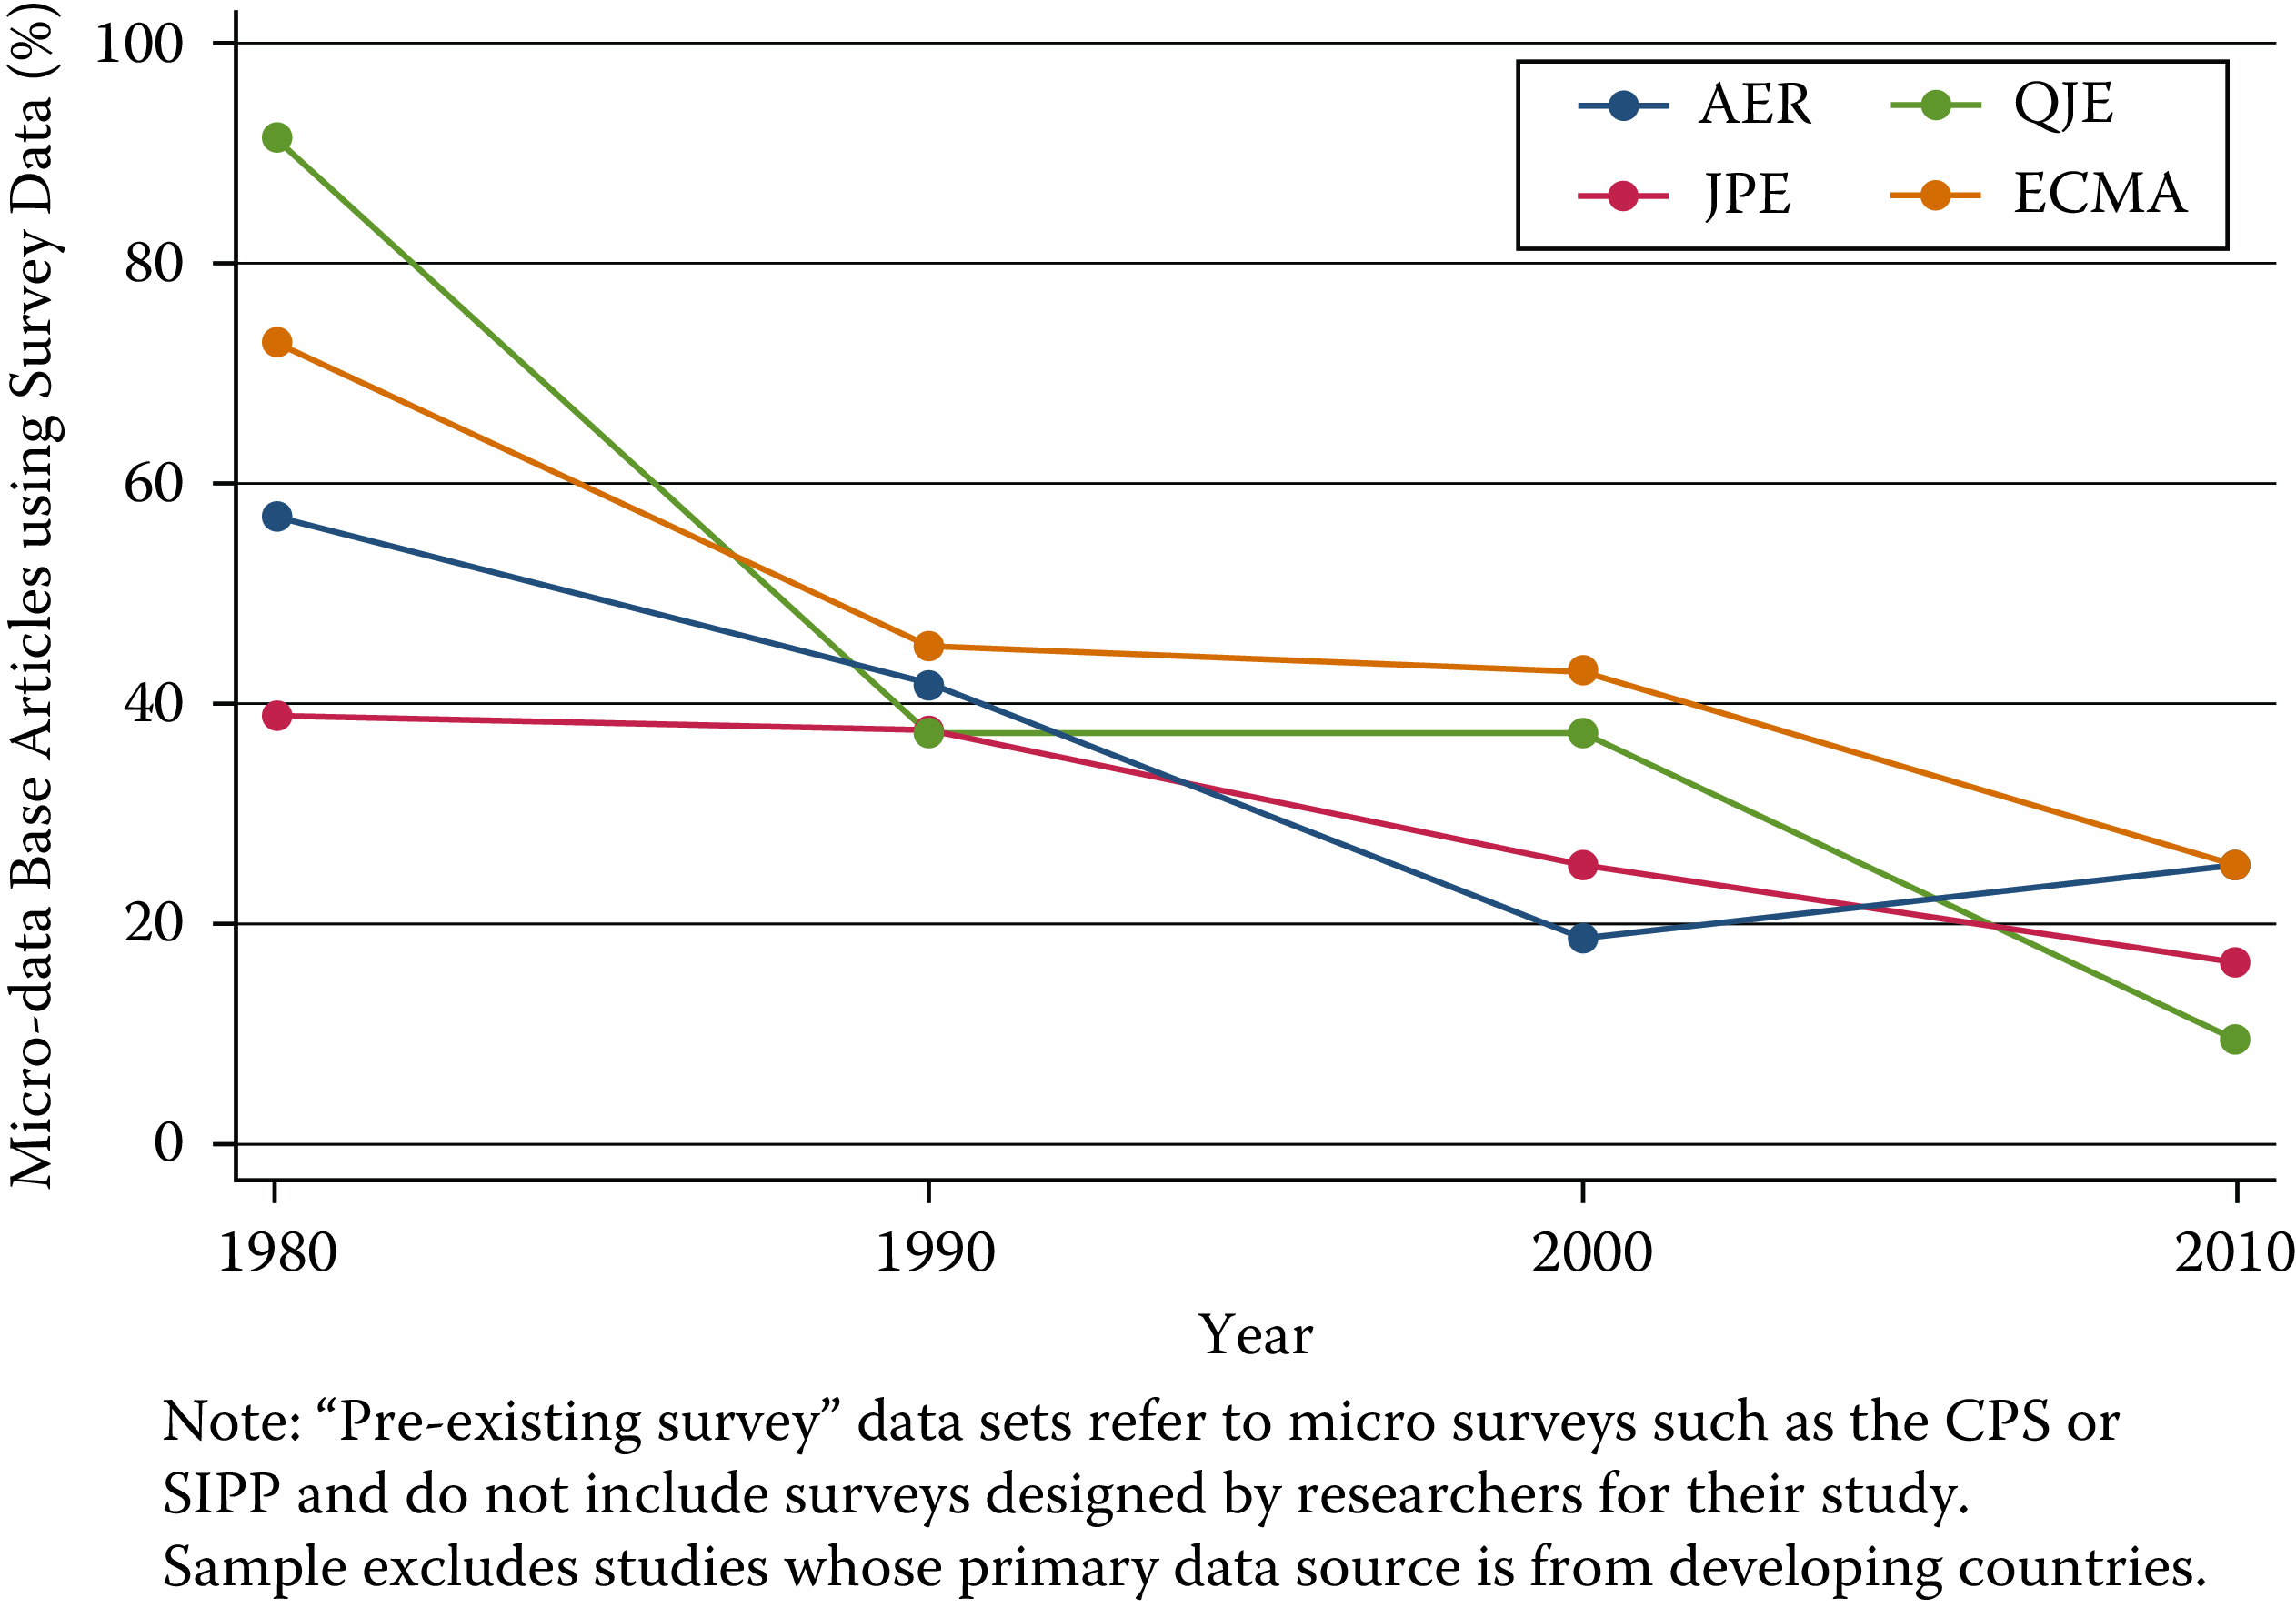
\includegraphics[width=0.7\linewidth]{ChapterIntro/figures/Figure1} 

}

\caption{Use of pre-existing survey data in publications in leading journals, 1980--2010 [@Chetty2012]}\label{fig:fig1}
\end{figure}

Policy has also changed. The Foundations of Evidence-based Policy Act,
which was signed into law in 2019, requires agencies to make use of
evidence and data in making policy decisions (Hart
\protect\hyperlink{ref-Hart}{2019}). The Act, together with the Federal
Data Strategy (Office of Management and Budget
\protect\hyperlink{ref-OfficeofManagementandBudget}{2019}) establishes
both Chief Data Officers to oversee the collection, use of and access to
many new types of data and a learning agenda to build the data science
capacity of agency staff.

And the jobs have changed. The new job title of ``data scientist'' is
highlighted in job advertisements on CareerBuilder.com and
Burningglass--- supplanting the demand for statisticians, economists,
and other quantitative social scientists if starting salaries are useful
indicators. At the federal level, the Office of Personnel Management
created a new data scientist job title.

The goal of this book is to provide social scientists with an
understanding of the key elements of this new science, value of the
tools and the opportunities for doing better work. The goal is also to
identify the many ways in which the analytical toolkits possessed by
social scientists can be brought to bear to enhance the generalizability
and usefulness of the work done by computer scientists.

We take a pragmatic approach, drawn on our experience of working with
data. Most social scientists set out to solve a real world social or
economic problem: they frame the problem, identify the data, do the
analysis, and then draw inferences. At all points, of course, the social
scientist needs to consider the ethical ramifications of her work,
particularly respecting privacy and confidentiality. The book follows
the same structure. We chose a particular problem---the link between
research investments and innovation---because that is a major social
science policy issue, and one in which social scientists have been
addressing using big data techniques.

\section{Defining big data and its value}\label{sec:1-2}

There are almost as many definitions of big data as there are new types
of data. One approach is to define big data as anything too big to fit
onto your computer.\footnote{This topic is discussed in more detail in
  Chapter \protect\hyperlink{chap:parallel}{Scaling up through Parallel
  and Distributed Computing}.} Another approach is to define it as data
with high volume, high velocity and great variety. We choose the
description adopted by the American Association of Public Opinion
Research: ``The term `'Big Data'' is an imprecise description of a rich
and complicated set of characteristics, practices, techniques, ethical
issues, and outcomes all associated with data'' (Japec et al.
\protect\hyperlink{ref-japec2015big}{2015}).

The value of the new types of data for social science is quite
substantial. Personal data have been hailed as the ``new oil'' of the
21st century (Greenwood et al.
\protect\hyperlink{ref-greenwood2014}{2014}). Policy-makers have found
that detailed data on human beings can be used to reduce crime (Lynch
\protect\hyperlink{ref-lynch2018}{2018}), improve health delivery (Pan
et al. \protect\hyperlink{ref-pan2017}{2017}) and manage cities better
(Glaeser \protect\hyperlink{ref-glaeser2019urban}{2019}). Society can
gain as well---much cited work shows data driven businesses were five
percent more productive and six percent more profitable than their
competitors (Brynjolfsson, Hitt, and Kim
\protect\hyperlink{ref-brynjolfsson2011strength}{2011}). Henry Brady
provides a succinct overview when he says ``Burgeoning data and
innovative methods facilitate answering previously hard-to-tackle
questions about society by offering new ways to form concepts from data,
to do descriptive inference, to make causal inferences, and to generate
predictions. They also pose challenges as social scientists must grasp
the meaning of concepts and predictions generated by convoluted
algorithms, weigh the relative value of prediction versus causal
inference, and cope with ethical challenges as their methods, such as
algorithms for mobilizing voters or determining bail, are adopted by
policy makers'' (Brady
\protect\hyperlink{ref-brady2019challenge}{2019}).

\begin{center}\rule{0.5\linewidth}{\linethickness}\end{center}

\textbf{Example: New potential for social science}

The billion prices project is a great example of how researchers can use
new web-scraping techniques to get online prices from hundreds of
websites and thousands of webpages to build datasets customized to fit
specific measurement and research needs in ways that were unimaginable
20 years ago (Cavallo and Rigobon
\protect\hyperlink{ref-cavallo2016billion}{2016}); other great examples
include the way in which researchers use text analysis of political
speeches to study political polarization (Peterson and Spirling
\protect\hyperlink{ref-peterson2018classification}{2018}) or of airbnb
postings to get new insights into racial discrimination (Edelman, Luca,
and Svirsky \protect\hyperlink{ref-edelman2017racial}{2017}).

\begin{center}\rule{0.5\linewidth}{\linethickness}\end{center}

But most interestingly, the new data can change the way we think about
behavior. For example, in a study of environmental effects on health,
researchers combined information on public school cafeteria deliveries
with children's school health records to show that simply putting water
jets in cafeterias reduced milk consumption and also reduced childhood
obesity (Schwartz et al.
\protect\hyperlink{ref-schwartz2016effect}{2016}). Another study which
shed new light into the role of peers on productivity found that the
productivity of a cashier increased if they were within eyesight of a
highly productive cashier but not otherwise (Mas and Moretti
\protect\hyperlink{ref-mas2009peers}{2009}). Studies like these show
ways in which clever use of data can lead to greater understanding of
the effects of complex environmental inputs on human behavior.

New types of data can also enable us to study to examine small
groups---the tails of a distribution---in a way that is not possible
with small data. Much of interest in human behavior is driven by those
tails---health care costs by small numbers of ill people (Stanton and
Rutherford \protect\hyperlink{ref-stanton2006high}{2006}), economic
activity and employment by a small number of firms (Evans
\protect\hyperlink{ref-evans1987tests}{1987}, Jovanovic
(\protect\hyperlink{ref-jovanovic1982selection}{1982})).

Our excitement about the value of new types of data must be accompanied
by a recognition of the lessons learned by statisticians and social
scientists from their past experience with surveys and small scale data
collection. The next sections provide a brief overview.

\section{The importance of inference}\label{sec:1.3}

It is critically important to be able to use data to generalize from the
data source to the population. That requirement exists, regardless of
the data source. Statisticians and social scientists have developed
methodologies for survey data to overcome problems in the
data-generating process. A guiding principle for survey methodologists
is the total survey error framework, and statistical methods for
weighting, calibration, and other forms of adjustment are commonly used
to mitigate errors in the survey process. Likewise for ``broken''
experimental data, techniques like propensity score adjustment and
principal stratification are widely used to fix flaws in the
data-generating process.

If we take a look across the social sciences, including economics,
public policy, sociology, management, (parts of) psychology and the
like, their scientific activities can be grouped into three categories
with three different inferential goals: Description, Causation and
Prediction.

\textbf{Description}

The job of many social scientists is to provide descriptive statements
about the population of interest. These could be univariate, bivariate
or even multivariate statements.

Usually descriptive statistics are created based on census data or
sample surveys to create some summary statistics like a mean, median or
a graphical distribution to describe the population of interest. In the
case of a census the work ends right there. With sample surveys the
point estimates come with measures of uncertainties (standard errors).
The estimation of standard errors has been worked out for most
descriptive statistics and most common survey designs, even complex ones
that include multiple layers of sampling and disproportional selection
probabilities (Hansen, Hurwitz, and Madow
\protect\hyperlink{ref-hansen1993sample}{1993}, Valliant, Dever, and
Kreuter (\protect\hyperlink{ref-valliant2013practical}{2013})).

\begin{center}\rule{0.5\linewidth}{\linethickness}\end{center}

\textbf{Example: Descriptive statistics}

The Census Bureau's American Community Survey (ACS) ``helps local
officials, community leaders, and businesses understand the changes
taking place in their communities. It is the premier source for detailed
population and housing information about our nation''
(\url{https://www.census.gov/programs-surveys/acs}). The summary
statistics are used by planners to allocate resources - but it's
important to pay attention to the standard errors, particularly for
small samples. For example, in one county (Autauga) in Alabama, with a
total population of about fifty-five thousand, the ACS estimates that
139 children under age 5 live in poverty---plus or minus 178! So the
plausible range is somewhere between 0 and 317 (Spielman and Singleton
\protect\hyperlink{ref-Spielman2015}{2015}).

\begin{center}\rule{0.5\linewidth}{\linethickness}\end{center}

Proper inference from a sample survey to the population usually depends
on knowing a) that everyone from the target population had the chance to
be included in the survey, and b) the selection probability for each
element in the population. The latter does not necessarily need to be
known prior to sampling, but eventually a probability is assigned for
each case. Getting the selection probabilities right is particularly
important when reporting totals (Lohr
\protect\hyperlink{ref-lohr2009sampling}{2009}). Unfortunately in
practice, samples that start out as probability samples can suffer from
a high rate of nonresponse. Because the survey designer cannot
completely control which units respond, the set of units that ultimately
respond cannot be considered to be a probability sample. Nevertheless,
starting with a probability sample provides some degree of comfort that
a sample will have limited coverage errors (nonzero probability of being
in the sample).

\textbf{Causation}

Identifying causal relationships is another common goal for social
science researchers (Hal R Varian
\protect\hyperlink{ref-varian2014big}{2014}). Ideally such explanations
stem from data that allow causal inference: typically randomized
experiments or strong non-experimental study designs. When examining the
effect of X on Y, knowing how cases were selected into the sample or
dataset is much less important to estimate causal effects than they are
for descriptive studies, e.g., population means. What is important is
that all elements of the inferential population have a chance to be
selected for the treatment (Imbens and Rubin
\protect\hyperlink{ref-imbens2015causal}{2015}). In the debate about
probability and non-probability surveys, this distinction is often
overlooked. Medical researchers have operated with unknown study
selection mechanisms for years: e.g, randomized trials that enroll very
selected samples.

\begin{center}\rule{0.5\linewidth}{\linethickness}\end{center}

\textbf{Example: New data and causal inference}

If the data generating process is not understood, resources can be badly
misallocated. Overreliance on, say, Twitter data, in targeting resources
after hurricanes can lead to the misallocation of resources towards
young, internet savvy people with cell-phones and away from elderly or
impoverished neighborhoods (Shelton et al.
\protect\hyperlink{ref-shelton2014mapping}{2014}). Of course, all data
collection approaches have had similar risks. Bad survey methodology led
the Literary Digest to incorrectly call the 1936 election (Squire
\protect\hyperlink{ref-squire19881936}{1988}). Inadequate understanding
of coverage, incentive and quality issues, together with the lack of a
comparison group, has hampered the use of administrative
records---famously in the case of using administrative records on crime
to make inference about the role of death penalty policy in crime
reduction (Donohue III and Wolfers
\protect\hyperlink{ref-donohue2006uses}{2006}).

\begin{center}\rule{0.5\linewidth}{\linethickness}\end{center}

In practice, regardless of how much data is available, researchers must
consider at least two things: 1) how well the results generalize to
other populations (Athey and Imbens
\protect\hyperlink{ref-athey2017state}{2017}) 2) whether the treatment
effect on the treated population is different than the treatment effect
in the full population of interest. New methods to address
generalizability are under development (DuGoff, Schuler, and Stuart
\protect\hyperlink{ref-dugoff2014generalizing}{2014}). While unknown
study selection probabilities usually makes it difficult to estimate
population causal effects, as long as we are able to model the selection
process there is no reason not to do causal inference from so-called
non-probability data.

\textbf{Prediction}

Forecasting or prediction tasks. The potential for massive amounts of
data to improve prediction is undeniable. However, just like the causal
inference setting, it is of utmost importance that we know the process
that generated the data, so that biases due to unknown or unobserved
systematic selection can be minimized. Predictive policing is a good
example of the challenges. The criminal justice system generates massive
amounts of data that can be used to better allocate police resources -
but if the data do not represent the population at large, the
predictions will be biased.

\begin{center}\rule{0.5\linewidth}{\linethickness}\end{center}

\textbf{Example: Learning from the flu}

``Five years ago in 2009, a team of researchers from Google announced a
remarkable achievement in one of the world's top scientific journals,
\emph{Nature}. Without needing the results of a single medical check-up,
they were nevertheless able to track the spread of influenza across the
US. What's more, they could do it more quickly than the Centers for
Disease Control and Prevention (CDC). Google's tracking had only a day's
delay, compared with the week or more it took for the CDC to assemble a
picture based on reports from doctors' surgeries. Google was faster
because it was tracking the outbreak by finding a correlation between
what people searched for online and whether they had flu symptoms.
\ldots{}

``Four years after the original \emph{Nature} paper was published,
\emph{Nature News} had sad tidings to convey: the latest flu outbreak
had claimed an unexpected victim: Google Flu Trends. After reliably
providing a swift and accurate account of flu outbreaks for several
winters, the theory-free, data-rich model had lost its nose for where
flu was going. Google's model pointed to a severe outbreak but when the
slow-and-steady data from the CDC arrived, they showed that Google's
estimates of the spread of flu-like illnesses were overstated by almost
a factor of two.

``The problem was that Google did not know---could not begin to
know---what linked the search terms with the spread of flu. Google's
engineers weren't trying to figure out what caused what. They were
merely finding statistical patterns in the data. They cared about
correlation rather than causation'' (Harford
\protect\hyperlink{ref-harford2014big}{2014}).

\begin{center}\rule{0.5\linewidth}{\linethickness}\end{center}

\section{The importance of understanding how data are
generated}\label{sec:1-4}

The costs of realizing the benefits of the new types of data are non
trivial. Even if data collection is cheap, the costs of cleaning,
curating, standardizing, integrating and using the new types of data are
substantial. In essence, just as with data from surveys, data still need
to be processed---cleaned, normalized, and variables coded---but this
needs to be done at scale.\footnote{This topic is discussed in more
  detail in Section \protect\hyperlink{sec:1-5}{New tools for new data}.}
But even once all of these tasks are completed, social scientists have a
key role in describing the quality of the data. This role is important,
because most data in the real world are noisy, inconsistent, and exhibit
missing values. Data quality can be characterized in multiple ways (see
Christen
(\protect\hyperlink{ref-christen2012data}{2012}\protect\hyperlink{ref-christen2012data}{b}),
National Academies of Sciences, Medicine, and others
(\protect\hyperlink{ref-national2018federal}{2018})), such as:

\begin{itemize}
\tightlist
\item
  Accuracy: How accurate are the attribute values in the data?
\item
  Completeness: Are the data complete?
\item
  Consistency: How consistent are the values in and between different
  database(s)?
\item
  Timeliness: How timely are the data?
\item
  Accessibility: Are all variables available for analysis?
\end{itemize}

In the social science world, the assessment of data quality is integral
to the production of the resultant statistics. That is not necessarily
easy when it comes to assessing new types of data. A good example of the
importance of understanding how data are generated came up in one of our
classes a couple of years ago, where class participants were asked to
develop employment measures for ex-offenders in the period after they
were released from prison (Kreuter, Ghani, and Lane
\protect\hyperlink{ref-Kreuter2019Change}{2019}).

For people working with surveys, the definition is already
preconstructed: in the Current Population Survey (CPS), respondents
asked about their work activity in the week covering the 12th of the
month. You're counted as employed if you have at least one hour of paid
work in that week (with some exceptions for family and farm work). But
the class participants were working with administrative records from the
Illinois Department of Employment Security and the Illinois Department
of Corrections (Kreuter, Ghani, and Lane
\protect\hyperlink{ref-Kreuter2019Change}{2019}). Those records provide
a report of all jobs in every quarter that each individual holds in the
state; when matched to data about formerly incarcerated individuals, it
can provide rich information about their employment patterns. A group of
class participants produced Figure \ref{fig:patternfig} - the white
boxes represent quarters in which an individual doesn't have a job and
the blue boxes represent quarters in which an individual does have a
job.

A quick look at the results is really interesting. First, the
participants present an entirely new, dynamic, way of looking at
employment - not just the relatively static CPS measure. Second, the
results are a bit shocking. Over 61 per cent of Illinois exoffenders did
not have a job in any of the 8 quarters after their release. Only 3.5
percent had a job in all of the quarters. This is where social
scientists and government analysts can contribute - because they know
how the data are generated. The matches between the two agencies are
done on (deidentified) Social Security numbers (SSNs). It's likely that
there are several gaps in that match. First, agency staff know that the
quality of SSNs in prisons is quite low, so that might be a reason for
the low match rate. Second, the match is only to Illinois jobs, and many
formerly incarcerated individuals could be working across state lines
(if allowed). Third, they may have gone to community college, or on
welfare, or back to prison. More data can be used to examine these
different possibilities - but we think it illustrates the value that
social scientists and subject matter experts provide to measuring the
quality issues we highlighted at the beginning of this section.

\begin{figure}

{\centering 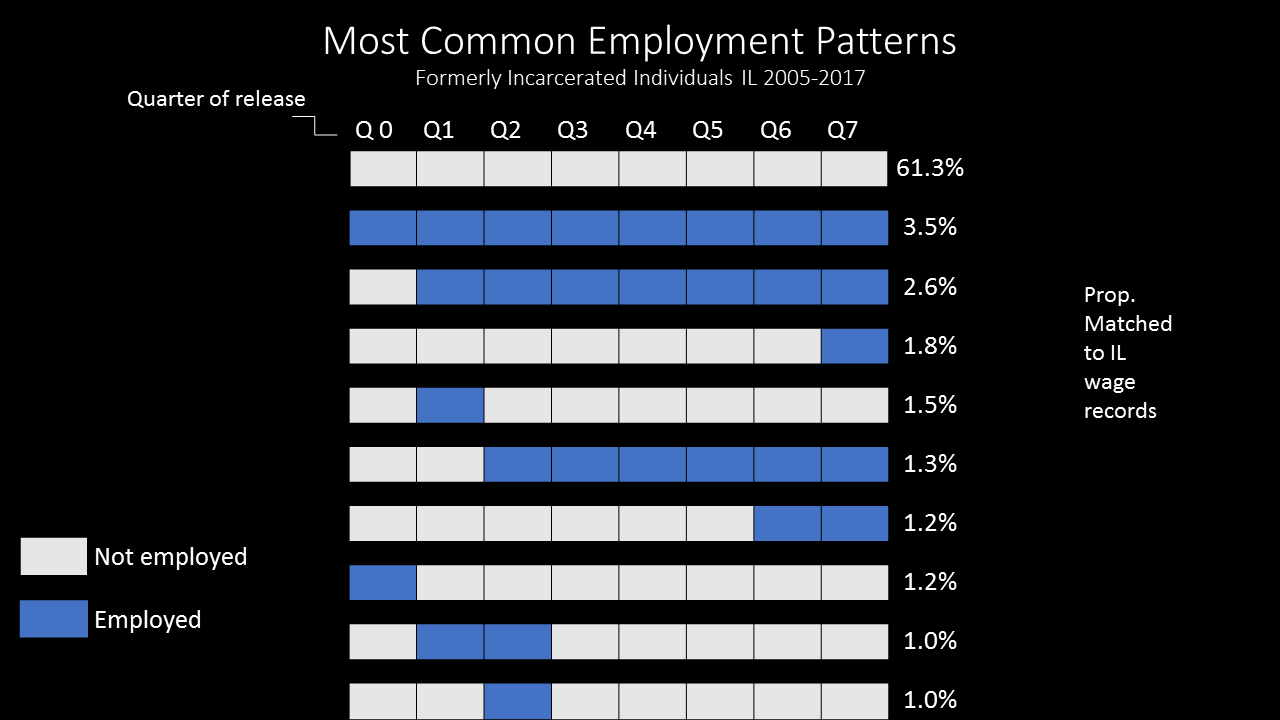
\includegraphics[width=0.9\linewidth]{ChapterIntro/figures/patterns} 

}

\caption{Most common employment patters, formerly incarcerated individuals in Illinois, 2005--2017}\label{fig:patternfig}
\end{figure}

\hypertarget{sec:1-5}{\section{New tools for new data}\label{sec:1-5}}

The new data sources that we have discussed frequently require working
at scales for which the social scientist's familiar tools are not
designed. Fortunately, the wider research and data analytics community
has developed a wide variety of often more scalable and flexible
tools---tools that we will introduce within this book.

Relational database management systems (DBMSs)\footnote{This topic is
  discussed in more detail in Chapter
  \protect\hyperlink{chap:db}{Databases}.} are used throughout business
as well as the sciences to organize, process, and search large
collections of structured data. NoSQL DBMSs are used for data that is
extremely large and/or unstructured, such as collections of web pages,
social media data (e.g., Twitter messages), sensor data, and clinical
notes. Extensions to these systems and also specialized single-purpose
DBMSs provide support for data types that are not easily handled in
statistical packages such as geospatial data, networks, and graphs.

Open source programming languages such as Python (used extensively
throughout this book) and R provide high-quality implementations of
numerous data analysis and visualization methods, from regression to
statistics, text analysis, network analysis, and much more. Finally,
parallel computing platforms such as Hadoop and Spark can be used to
harness parallel computer clusters for extremely large data sets and
computationally intensive analyses.

These various components may not always work together as smoothly as do
integrated packages such as SAS, SPSS, and Stata, but they allow
researchers to take on problems of greater scale and complexity.
Furthermore, they are developing at a tremendous rate as the result of
work by thousands of people worldwide. For these reasons, the modern
social scientist needs to be familiar with their capabilities.

\section{\texorpdfstring{The book's ``use
case''}{The book's use case}}\label{sec:1-6}

This book is about the uses of big data in social science. Our focus is
on working through the use of data as a social scientist normally
approaches research. That involves thinking through how to use such data
to address a question from beginning to end, and thereby learning about
the associated tools---rather than simply engaging in coding exercises
and then thinking about how to apply them to a potpourri of social
science examples.

There are many examples of the use of big data in social science
research. Our challenge in designing the book was to find a use case
that was interesting, that didn't require access to confidential
micro-data, that made use of all the methods and tools that a typical
researcher might want to learn about, and that could be applied to most
of the many other use cases that might be of interest to other
instructors (such as criminal justice, health care, welfare, education
or economic development). We chose to make use of the great surge of
interest in examining the impact of investments in research and
development on economic and social outcomes, and which constitutes one
of the first large-scale big data social science data infrastructures.
Many of the data sources are public, and it is those that are used in
this book.

We think the question should also be of broad interest to many potential
users, even if they're not subject matter specialists. The surge of
interest was in response to a call from the President's Science Advisor
(Jack Marburger) for a \emph{science of science policy} (Marburger
\protect\hyperlink{ref-marburger2005wanted}{2005}). He wanted a
scientific response to the questions that he was asked about the impact
of investments in science.

\begin{center}\rule{0.5\linewidth}{\linethickness}\end{center}

\textbf{Example: The Science of Science Policy}

Marburger made some very insightful points during his tenure as Science
Advisor. He was sceptical of the calls for more and more investment in
science, particularly of the European push for 3\% of GDP to be
allocated to research and development. He wanted to both understand and
be able to explain what would be the returns to that kind of
expenditure. In a very famous editorial, he asked (Marburger
\protect\hyperlink{ref-marburger2005wanted}{2005}): ``How much should a
nation spend on science? What kind of science? How much from private
versus public sectors? Does demand for funding by potential science
performers imply a shortage of funding or a surfeit of performers? These
and related science policy questions tend to be asked and answered today
in a highly visible advocacy context that makes assumptions that are
deserving of closer scrutiny. A new `science of science policy' is
emerging, and it may offer more compelling guidance for policy decisions
and for more credible advocacy. \ldots{}

``Relating R\&D to innovation in any but a general way is a tall order,
but not a hopeless one. We need econometric models that encompass enough
variables in a sufficient number of countries to produce reasonable
simulations of the effect of specific policy choices. This need won't be
satisfied by a few grants or workshops, but demands the attention of a
specialist scholarly community. As more economists and social scientists
turn to these issues, the effectiveness of science policy will grow, and
of science advocacy too.''

\begin{center}\rule{0.5\linewidth}{\linethickness}\end{center}

In order to answer his question, an entire research field developed that
pulled together relevant data from a wide variety of different sources
using widely differing methodologies and approaches. They addressed
challenges often faced by social science and computer science
researchers trying to use new data to answer important
questions---namely that inputs, outputs and outcomes are not generated
or combined in a systematic fashion, even though producing consistent
and reliable answers to stakeholder requests requires the use of common
data sources and standardized methodologies. They were able to pull
together new digital sources of data and apply modern technologies to
analyze them. In the book we use three main examples to show how this
was done. The first is to describe \textbf{what} research is being done,
using data produced from multiple agencies on grand funding. The second
is to use award and patent administrative records to describe
\textbf{who} is doing the research (and \textbf{with whom}). The third
is to use patent data to describe \textbf{what results} the funding has
generated (Weinberg et al.
\protect\hyperlink{ref-weinberg2014science}{2014}, Lane et al.
(\protect\hyperlink{ref-Lane2018}{2018}))

Showing how those challenges can be addressed fits in with the goal of
the book. The focus is to highlight how to use new digital technologies
to capture the data needed to understand and address a set of questions,
with an illustrative focus on the broad results of Federal Science and
Technology investments. We are able to draw on the public availability
of a wide variety of research inputs, such as federal grant information,
and some outputs, particularly patent data. We are also able to draw on
new and more accurate methods exist for reliably attributing research
products to researchers, a nontrivial task due to considerable ambiguity
in author names (Han et al. \protect\hyperlink{ref-han2004two}{2004},
Smalheiser and Torvik
(\protect\hyperlink{ref-smalheiser2009author}{2009}), Li et al.
(\protect\hyperlink{ref-li2014disambiguation}{2014}), Kim, Khabsa, and
Giles (\protect\hyperlink{ref-kim2016inventor}{2016})). Figure
\ref{fig:fig2} provides an abstract representation of the empirical
approach that is needed: data about grants, the people who are funded on
grants, and the subsequent scientific and economic activities and shows.

First, data must be captured on what is funded, and since the data are
in text format, computational linguistics tools must be applied
(\protect\hyperlink{chap:text}{Text Analysis}). Second, data must be
captured on who is funded, and how they interact in teams, so network
tools and analysis must be used
(\protect\hyperlink{chap:networks}{Networks: The Basics}). Third,
information about the type of results must be gleaned from the web and
other sources (\protect\hyperlink{chap:web}{Working with Web Data and
APIs}).

Finally, the disparate complex data sets need to be stored in databases
(\protect\hyperlink{chap:db}{Databases}), integrated
(\protect\hyperlink{chap:link}{Record Linkage}), analyzed
(\protect\hyperlink{chap:ml}{Machine Learning}), and used to make
inferences (\protect\hyperlink{chap:errors}{Data Quality and Inference
Errors}).

\begin{figure}

{\centering 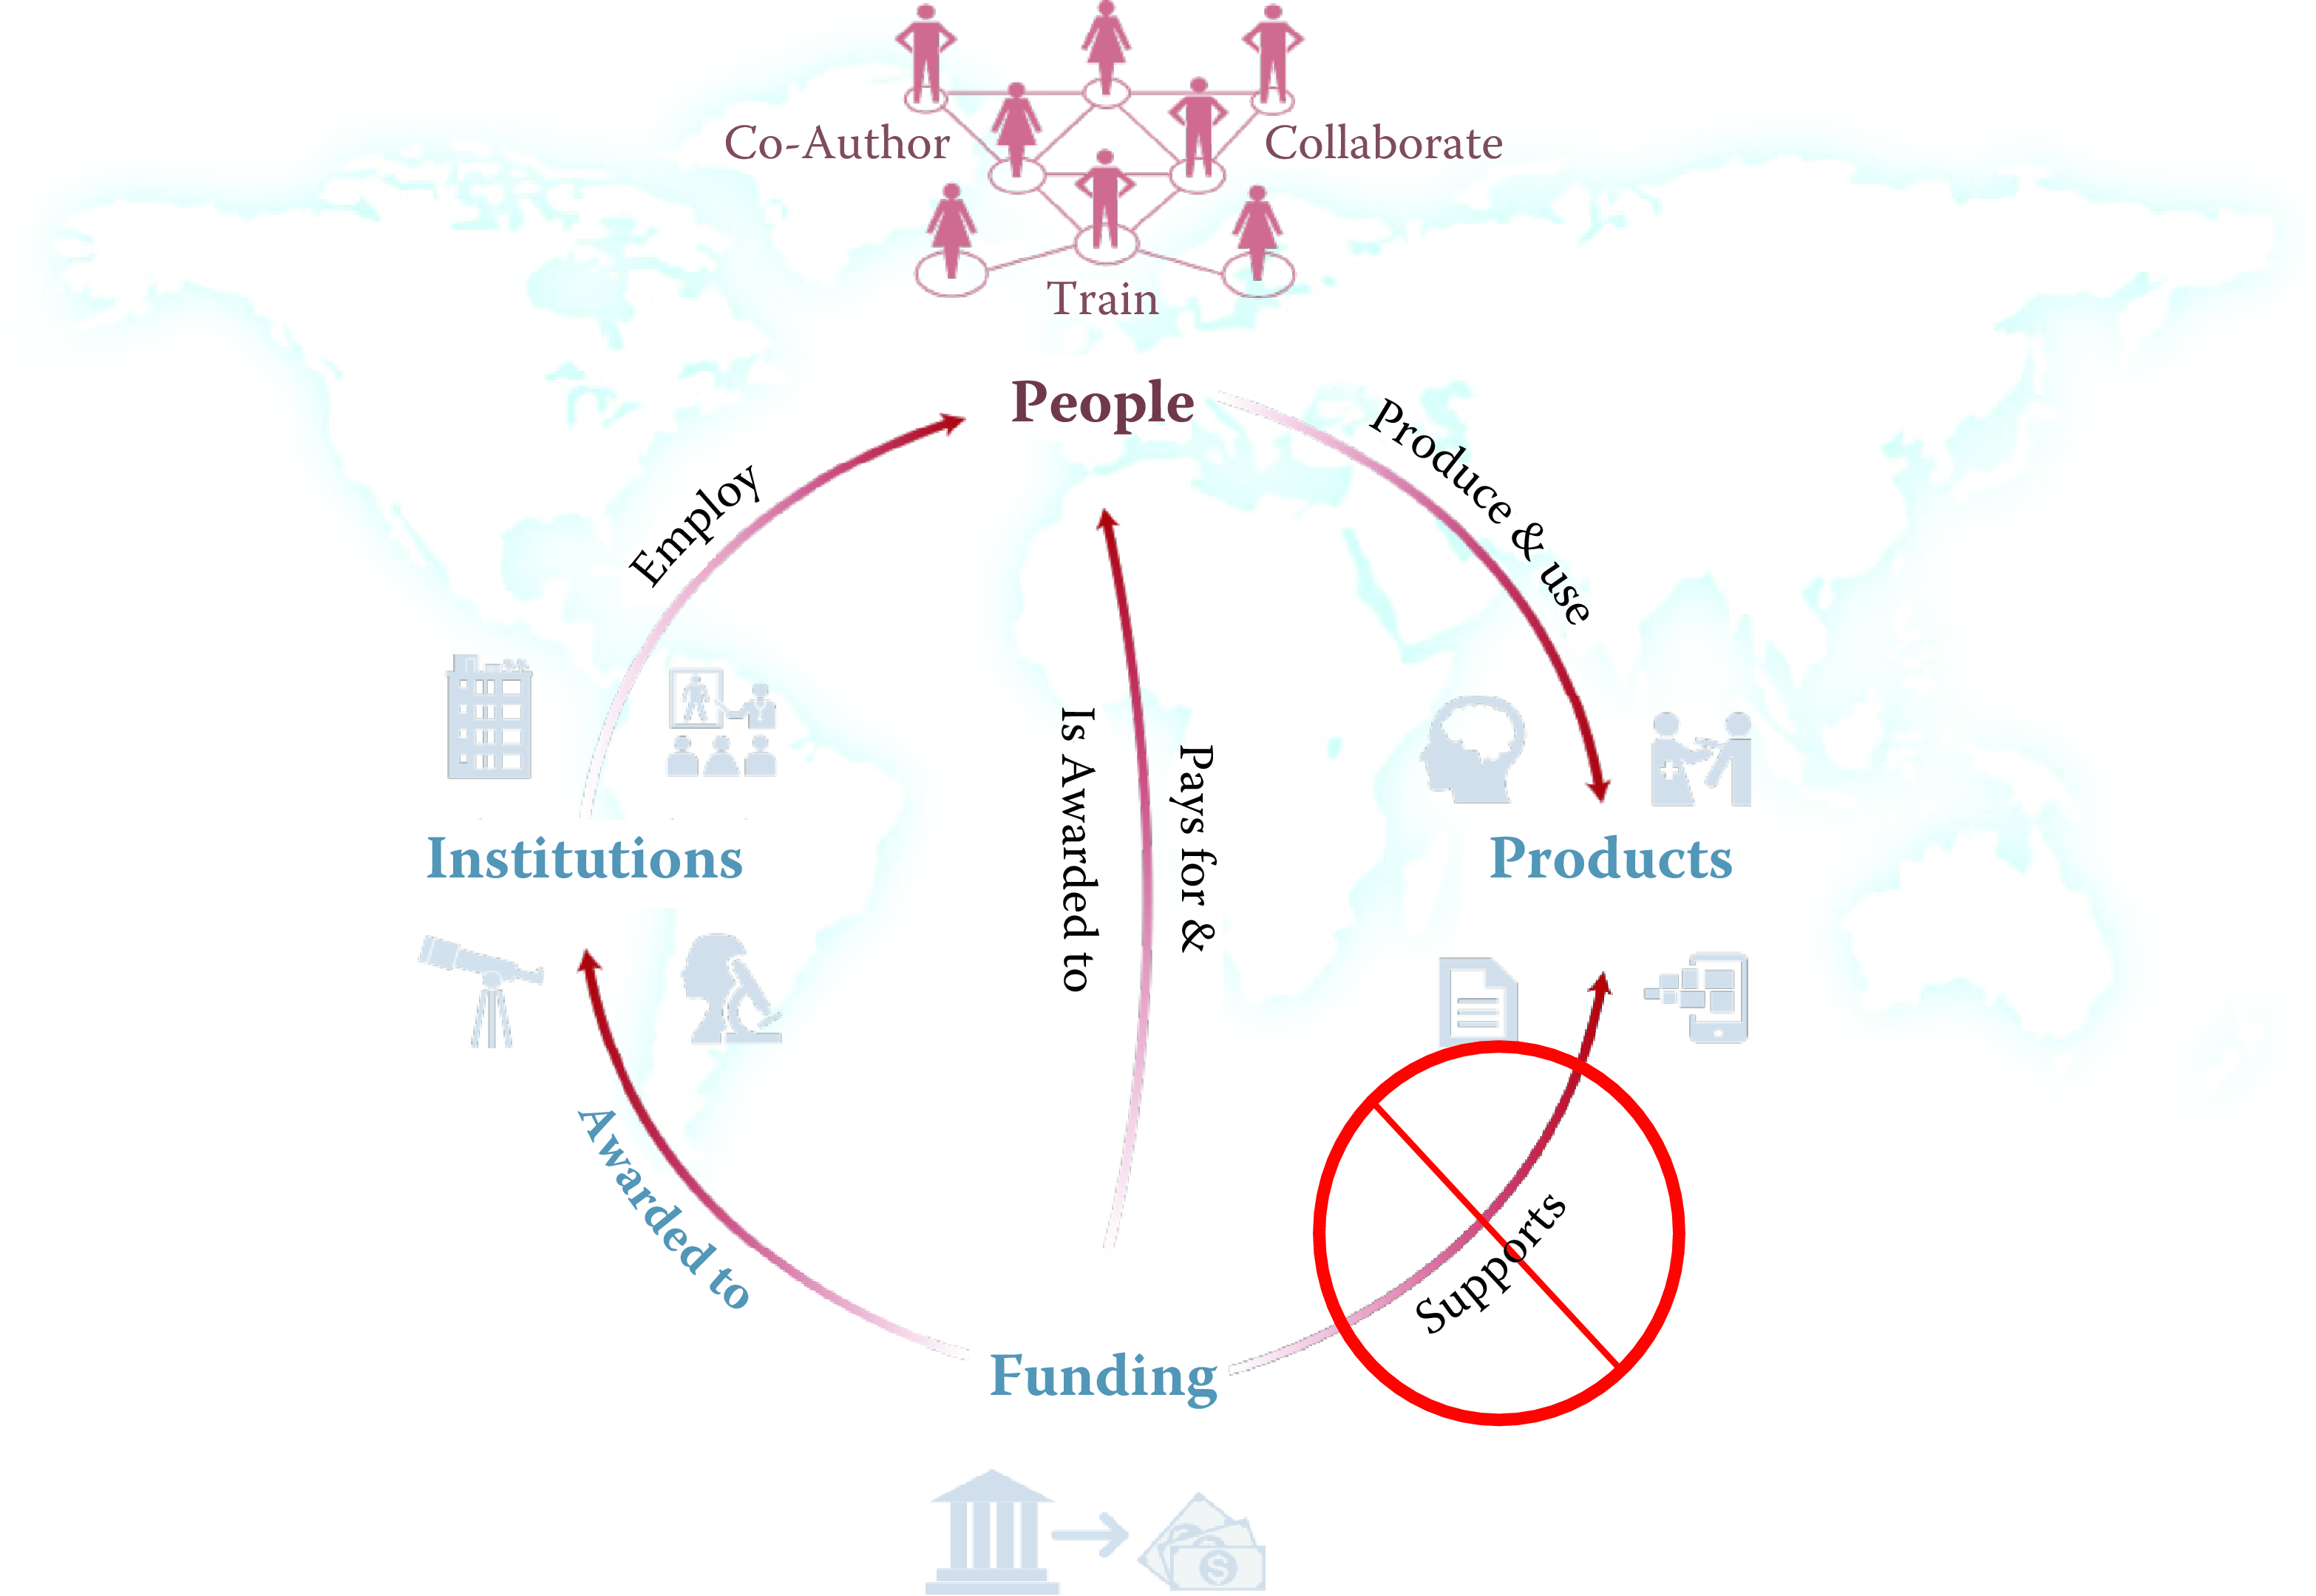
\includegraphics[width=0.7\linewidth]{ChapterIntro/figures/figure_cameron} 

}

\caption{A visualization of the complex links between what and who is funded, and the results; tracing the direct link between funding and results is misleading and wrong}\label{fig:fig2}
\end{figure}

The use case serves as the thread that ties many of the ideas together.
Rather than asking the reader to learn how to code ``hello world,'' we
build on data that have been put together to answer a real-world
question, and provide explicit examples based on that data. We then
provide examples that show how the approach generalizes.

For example, the text analysis chapter
(\protect\hyperlink{chap:text}{Text Analysis}) shows how to use natural
language processing to describe \emph{what} research is being done,
using proposal and award text to identify the research topics in a
portfolio (Talley, Newman, Mimno, Herr II, et al.
\protect\hyperlink{ref-talley2011database}{2011}; Evans and Foster
\protect\hyperlink{ref-Evans2011}{2011}). But then it also shows how the
approach can be used to address a problem that is not just limited to
science policy---the conversion of massive amounts of knowledge that is
stored in text to usable information.

Similarly, the network analysis chapter
(\protect\hyperlink{chap:networks}{Networks: The Basics}) gives specific
examples using the UMETRICS data and shows how such data can be used to
create new units of analysis---the networks of researchers who do
science, and the networks of vendors who supply research inputs. It also
shows how networks can be used to study a wide variety of other social
science questions.

In another example, we use APIs\footnote{Application Programming
  Interfaces} provided by publishers to describe the results generated
by research funding in terms of publications and other measures of
scientific impact, but also provide code that can be repurposed for many
similar APIs.

And, of course, since all these new types of data are provided in a
variety of different formats, some of which are quite large (or
voluminous), and with a variety of different timestamps (or velocity),
we discuss how to store the data in different types of data formats.

\begin{center}\rule{0.5\linewidth}{\linethickness}\end{center}

\textbf{BOX}

Much more information is available at the Institute for Research on
Innovation and Science (IRIS, \url{https://iris.isr.umich.edu/}) at the
University of Michigan. The Institute has extended the data
infrastructure to bring together both confidential and public data in a
secure environment. They have worked with universities interested in
documenting the results of their grant funding, they are able to trace
the spending of almost 400,000 grants to over 600,000 individuals and
820,000 vendors---and show the direct effects on that funding on their
subsequent scientific and economic activity (Institute For Research On
Innovation And Science (IRIS) Research
\protect\hyperlink{ref-InstituteForResearchOnInnovationAndScienceIRISResearch2019}{2019}).
To date, over 100 researchers from dozens of institutions have worked
with the new data infrastructure to provide an empirical response to
Marburger's call.

\begin{center}\rule{0.5\linewidth}{\linethickness}\end{center}

Although we focus on one particular use case, the methods covered in
this book are broadly applicable across a variety of policy
areas---indeed, we have used this book to teach classes in such fields
as education, criminal justice, workforce and economic development and
social services (\url{https://coleridgeinitiative.org/training}).

The methods have been used to answer questions such as:

\begin{itemize}
\item
  `What are the earnings and employment outcomes of individuals
  graduating from two and four year colleges?'
\item
  `How does placement in different types of firms change the likelihood
  that the formerly incareratedwill recidivate?'
\item
  `What factors increase the likelihood that welfare recipients on TANF
  (Temporary Asistance to Needy Families) will leave welfare?'
\end{itemize}

and

\begin{itemize}
\tightlist
\item
  `How do regulatory agencies move from reactive, complaint-based,
  health and safety inspections for workplaces and housing to a more
  proactive approach that focuses on prevention?'
\end{itemize}

\begin{center}\rule{0.5\linewidth}{\linethickness}\end{center}

\textbf{BOX}

Building data science skills to support state and local efforts to
become more data driven in the provision of human services.

The Offices of Family Assistance Office and of Planning, Research, and
Evaluation in the Department of Health and Human Services'
Administration for Children and Families set up a TANF data
collaborative (\url{https://www.tanfdata.org/}) to help professionals at
TANF and related human services agencies develop key data science
skills. The focus is on teaching participants how to scope a problem, do
record linkage, apply machine learning and visualization tools and learn
about privacy issues when working with confidential data.

\begin{center}\rule{0.5\linewidth}{\linethickness}\end{center}

\section{The structure of the book}\label{the-structure-of-the-book}

We organize the book in three parts, based around the way social
scientists approach doing research. The first set of chapters addresses
the new ways to capture, curate, and store data. The second set of
chapters describes what tools are available to process and analyze data.
The last set deals with the appropriate handling of data on individuals
and organizations as well as what inferences can be drawn from the data
and the analysis that was done. Of course, we assume that before
starting with the data and analysis, we have spent time on formulating
the problem or question that is being addressed. We don't cover that in
this book but refer readers to resources such as ``Data Science Project
Scoping''\footnote{\url{http://www.dssgfellowship.org/2016/10/27/scoping-data-science-for-social-good-projects/}}
for more information.

\begin{figure}

{\centering 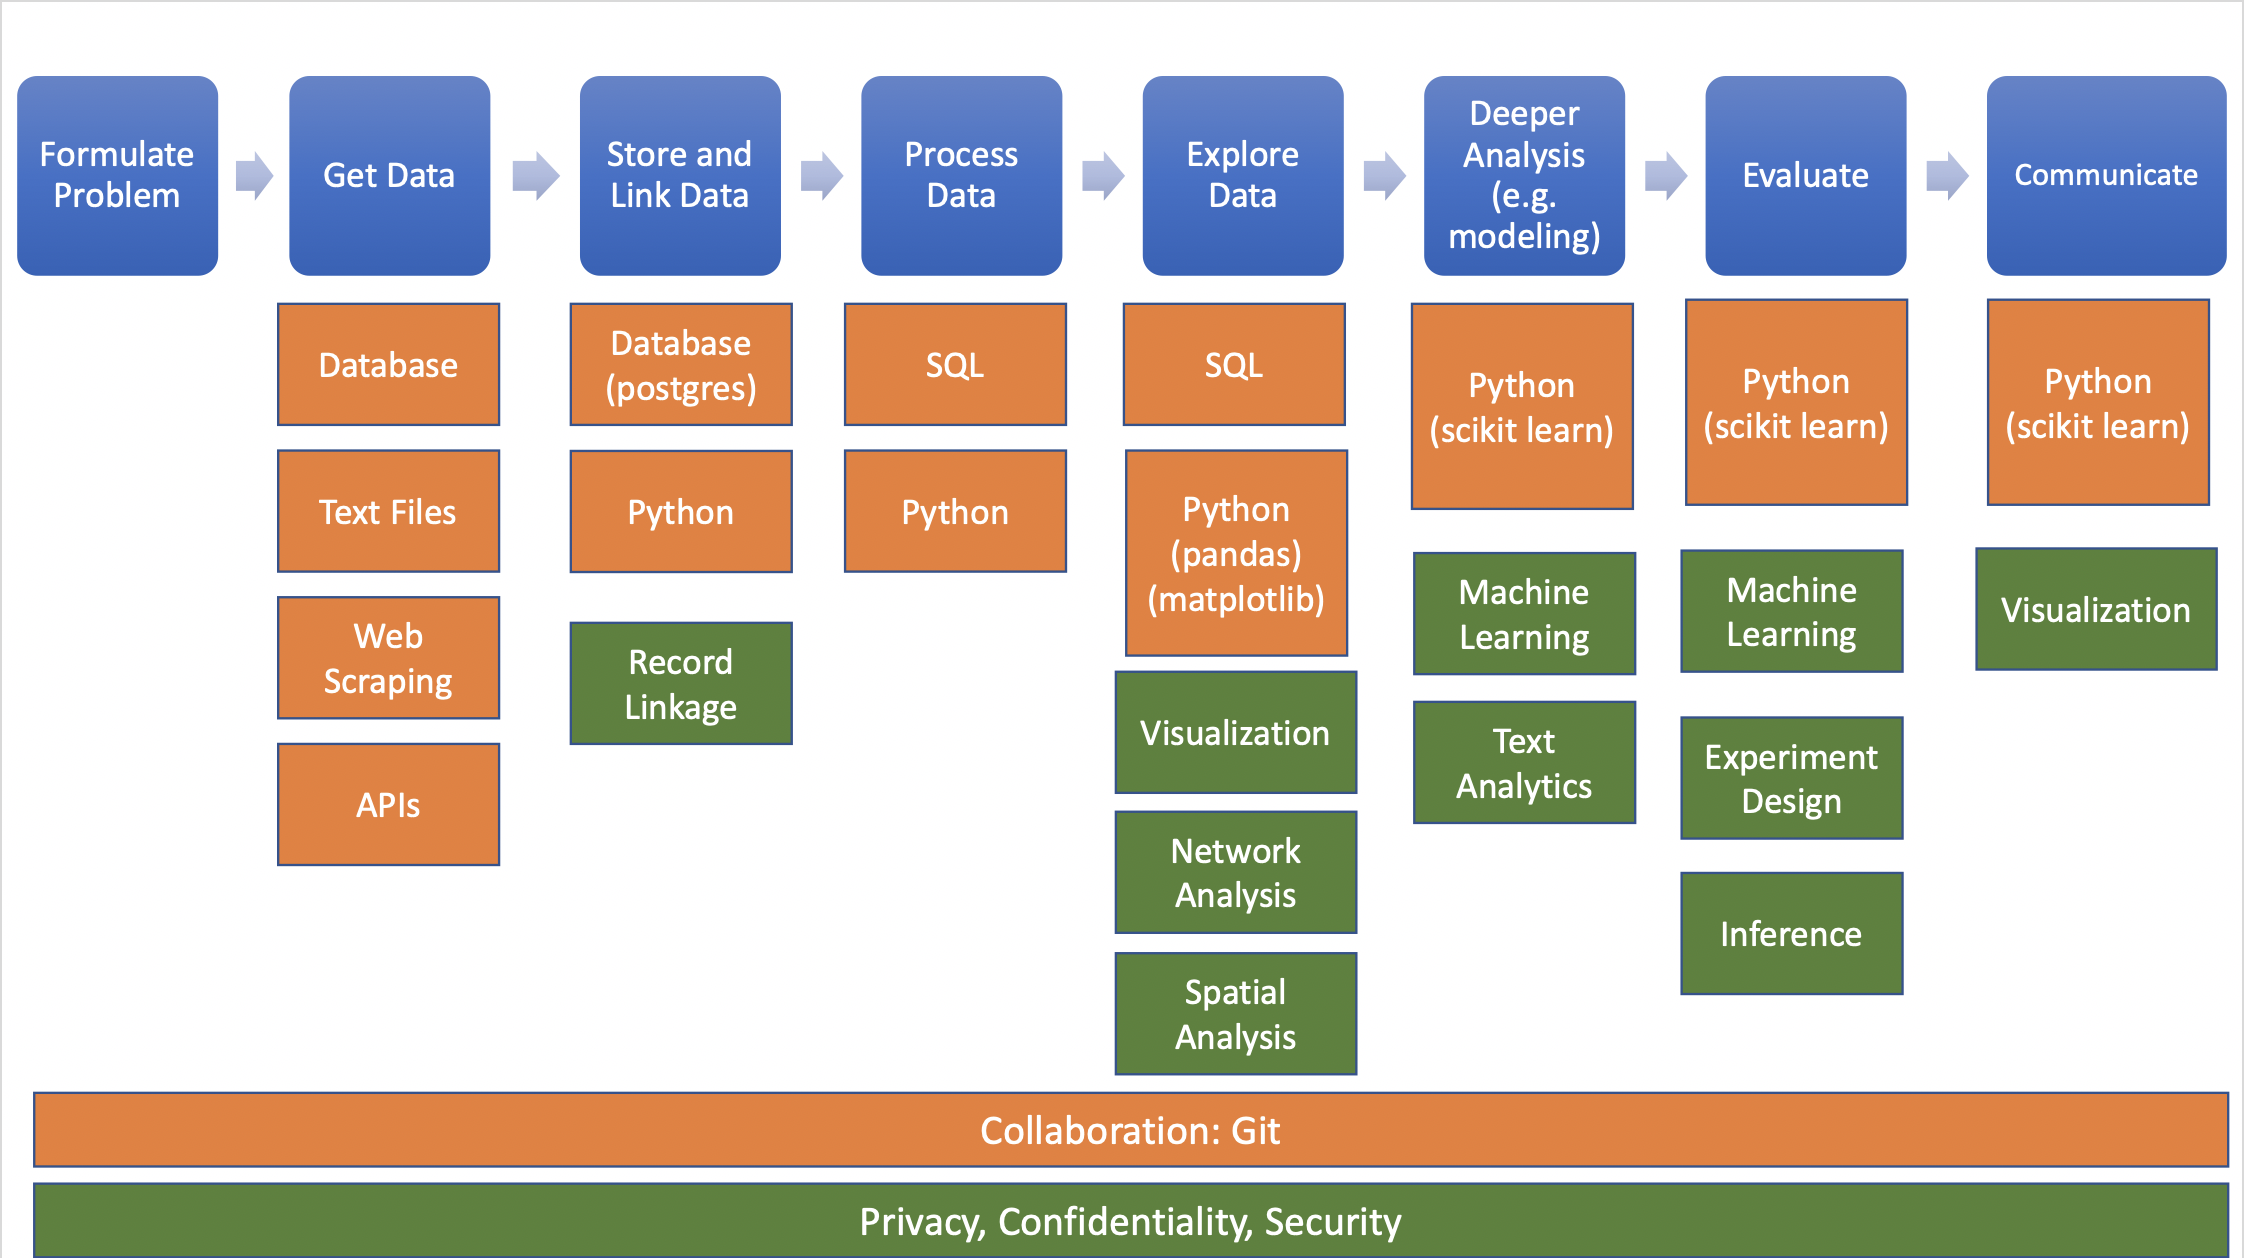
\includegraphics[width=1\linewidth]{ChapterIntro/figures/projectflow} 

}

\caption{The data science project workflow. Blue represents each step in the project, orange represents the tools used in that step, and green represents the methods for analysis.}\label{fig:projectfig}
\end{figure}

\subsection{Part I: Capture and
curation}\label{part-i-capture-and-curation}

The four chapters in Part I (see Figure \ref{fig:fig3}) tell you how to
collect, store, link, and manage data.

\protect\hyperlink{chap:web}{Working with Web Data and APIs} describes
how to extract information from data sources on the Web, including
social media. The particular application will be to develop links to
authors' articles on Twitter using PLOS articles and to pull information
about authors and articles from web sources by using an API. You will
learn how to retrieve link data from bookmarking services, citations
from Crossref, links from Facebook, and information from news coverage.
In keeping with the social science grounding that is a core feature of
the book, the chapter discusses what data can be captured from online
sources, what is potentially reliable, and how to manage data quality
issues.

This data differs from survey data in that we must typically combine
data from multiple sources to get a complete picture of the activities
of interest. Although computer scientists may sometimes simply ``mash''
data sets together, social scientists are rightfully concerned about
issues of missing links, duplicative links, and erroneous links.
\protect\hyperlink{chap:link}{Record Linkage} provides an overview of
traditional rule-based and probabilistic approaches to data linkage, as
well as machine learning approaches that are more adaptive and tunable.

Once data have been collected and linked, it is necessary to store and
organize it. Social scientists are used to working with one analytical
file, often in statistical software tools such as SAS or Stata.
\protect\hyperlink{chap:db}{Databases} describes different approaches to
storing data in ways that facilitate rapid, scalable, and reliable
exploration and analysis.

Big data is sometimes defined as data that are too big to fit onto the
analyst's computer. \protect\hyperlink{chap:parallel}{Scaling up through
Parallel and Distributed Computing} provides an overview of programming
techniques that facilitate the scalable use of data (often using
parallel computing). While the focus is on one of the most widely used
big data programming paradigms and its most popular implementation,
Apache Hadoop, the goal of the chapter is to provide a conceptual
framework to the key challenges that the approach is designed to
address.

\begin{figure}

{\centering 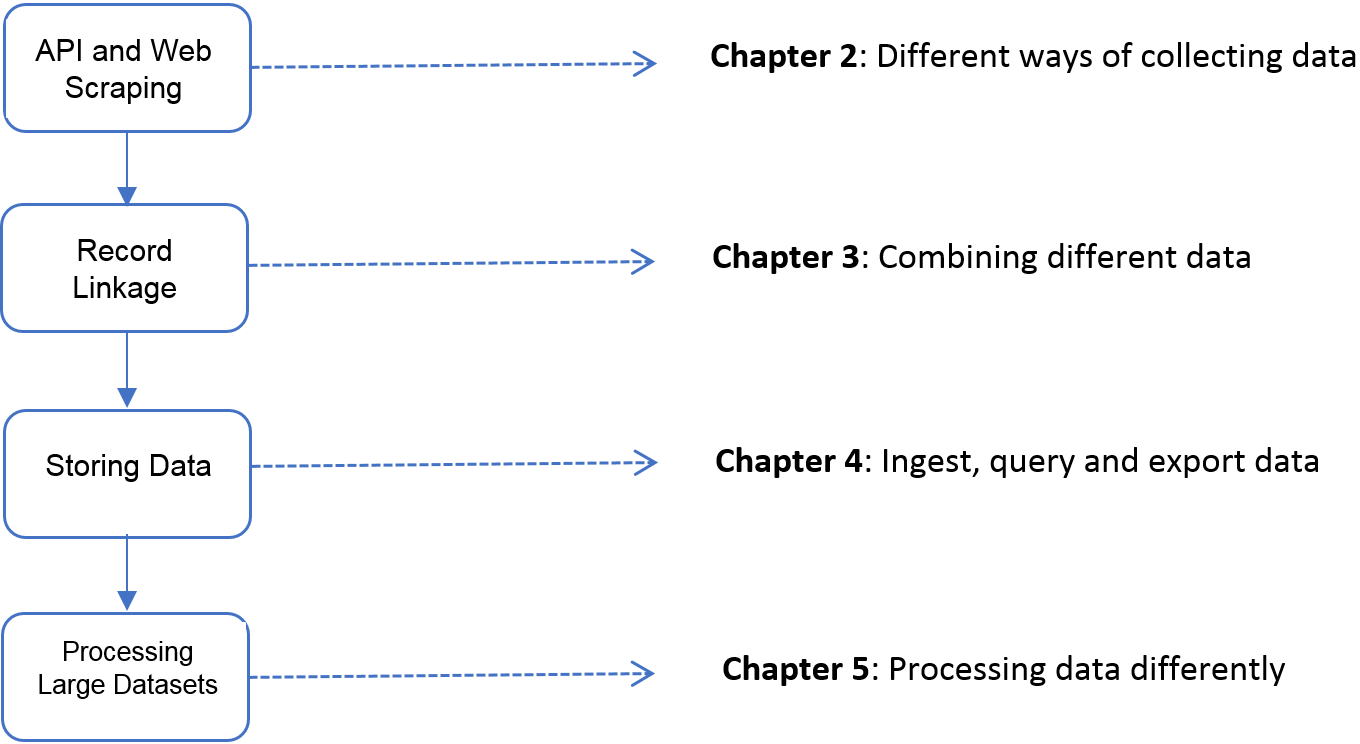
\includegraphics[width=0.9\linewidth]{ChapterIntro/figures/Figure2_new} 

}

\caption{The four chapters of Part I focus on *data capture* and *curation*}\label{fig:fig3}
\end{figure}

\subsection{Part II: Modeling and
analysis}\label{part-ii-modeling-and-analysis}

The four chapters in Part II (see Figure \ref{fig:fig4}) introduce four
of the most important tools that can be used by social scientists to do
new and exciting research: information visualization, machine learning,
text analysis, and social network analysis.

\protect\hyperlink{chap:viz}{Information Visualization} introduces
information visualization methods and describes how you can use those
methods to explore data and communicate results so that data can be
turned into interpretable, actionable information. There are many ways
of presenting statistical information that convey content in a rigorous
manner. The goal of this chapter is to explore different approaches and
examine the information content and analytical validity of the different
approaches. It provides an overview of effective visualizations. Using
visualization already in early analysis stages is key to a good
understanding of data quality and potential pitfalls.

\protect\hyperlink{chap:ml}{Machine Learning} introduces machine
learning methods. It shows the power of machine learning in a variety of
different contexts, particularly focusing on clustering, classification,
and prediction. You will get an overview of basic approaches and how
those approaches are applied. The chapter builds from a conceptual
framework on how to formulate social science problems as machine
learning problems, how to perform machine learning analysis, and how to
evaluate the analysis. These concepts are then translated into code to
ensure that the analysis can be put into practical use by social science
researchers and practitioners.

\protect\hyperlink{chap:text}{Text Analysis} describes how social
scientists can make use of text data through text analysis and natural
language processing methods. Dealing with text and analysing text is not
new to social scientists. What is different these days is that the vast
amounts of data that are stored in documents can now be analyzed and
searched and analyzed at scale, so that different types of information
can be retrieved. Documents (and the underlying activities of the
entities that generated the documents) can be categorized into topics or
fields as well as summarized. In addition, machine translation can be
used to compare documents in different languages.

Social scientists are typically interested in describing the activities
of individuals and organizations (such as households and firms) in a
variety of economic and social contexts. The frames within which data
are collected have typically been generated from tax or other
programmatic sources. The new types of data permit new units of
analysis---particularly network analysis---largely enabled by advances
in mathematical graph theory. Thus,
\protect\hyperlink{chap:networks}{Networks: The Basics} describes how
social scientists can use network theory to generate measurable
representations of patterns of relationships connecting entities. As the
author points out, the value of the new framework is not only in
constructing different right-hand-side variables but also in studying an
entirely new unit of analysis that lies somewhere between the largely
atomistic actors that occupy the markets of neo-classical theory and the
tightly managed hierarchies that are the traditional object of inquiry
of sociologists and organizational theorists.

\begin{figure}

{\centering 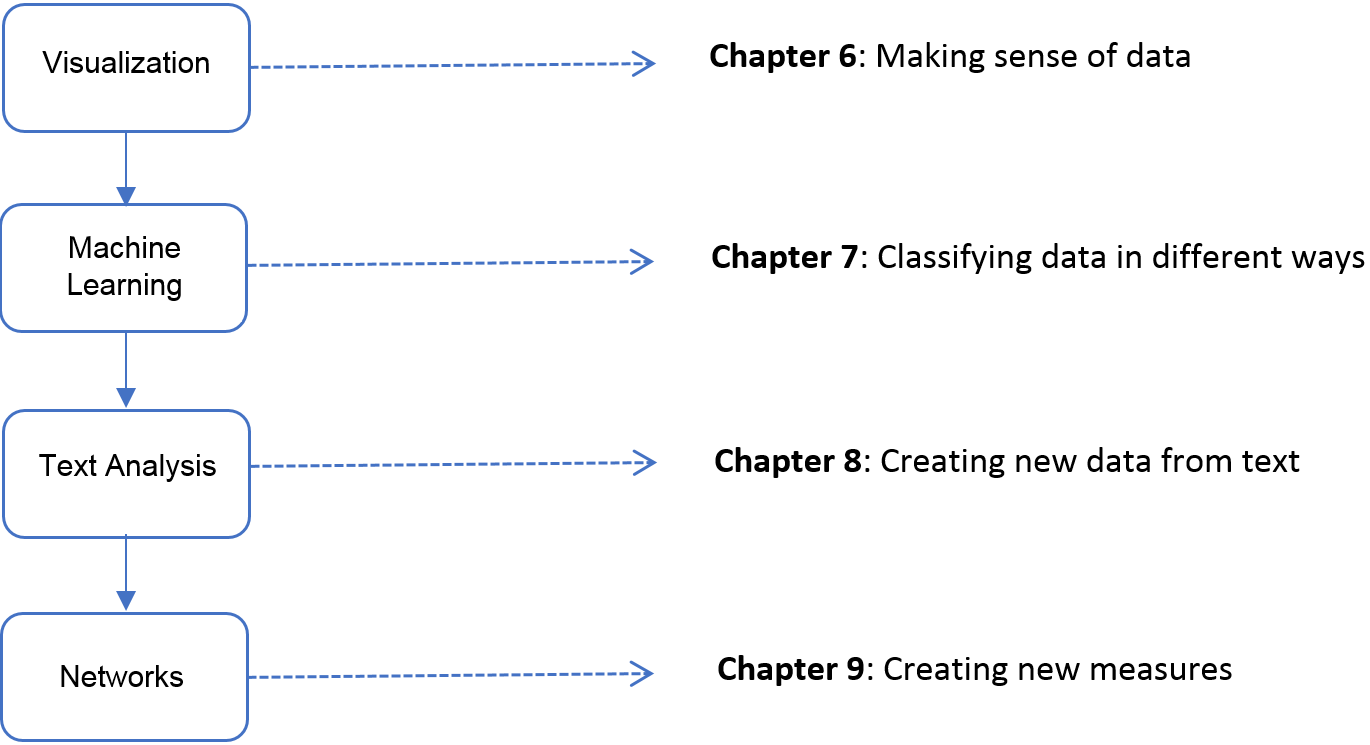
\includegraphics[width=0.9\linewidth]{ChapterIntro/figures/Figure3_new} 

}

\caption{The four chapters in Part II focus on data *modeling* and *analysis*}\label{fig:fig4}
\end{figure}

\subsection{Part III: Inference and
ethics}\label{part-iii-inference-and-ethics}

The three chapters in Part III (see Figure \ref{fig:fig5}) cover three
advanced topics relating to data inference and ethics---errors and
inference, bias, and privacy and confidentiality---and introduce the
workbooks that provide access to the practical exercises associated with
the text.

\protect\hyperlink{chap:errors}{Data Quality and Inference Errors} deals
with inference and the errors associated with big data. Social
scientists know only too well the cost associated with bad data---we
highlighted the classic \emph{Literary Digest} example in the
introduction to this chapter, as well as the more recent Google Flu
Trends. Although the consequences are well understood, the new types of
data are so large and complex that their properties often cannot be
studied in traditional ways. In addition, the data generating function
is such that the data are often selective, incomplete, and erroneous.
Without proper data hygiene, errors can quickly compound. This chapter
provides a systematic way to think about the error framework in a big
data setting.

\protect\hyperlink{chap:bias}{Bias and Fairness} Interest in algorithmic
fairness and bias has been growing recently, but it's easy to get lost
in the large number of definitions and metrics. There are many
different, often competing, ways to measure whether a given model and
the resulting system is ``fair''. In this chapter, we provide an
overview of these metrics along with some concrete examples to help
navigate these concepts and understand the trade-offs involved in
choosing to optimize one metric over others.

\protect\hyperlink{chap:privacy}{Privacy and Confidentiality} addresses
the issue that sits at the core of any study of human beings---privacy
and confidentiality. In a new field, like the one covered in this book,
it is critical that many researchers have access to the data so that
work can be replicated and built on---that there be a scientific basis
to data science. Yet the rules that social scientists have traditionally
used for survey data, namely anonymity and informed consent, no longer
apply when the data are collected in the wild. This concluding chapter
identifies the issues that must be addressed for responsible and ethical
research to take place.

Finally, \protect\hyperlink{chap:workbooks}{Workbooks} provides an
overview of the practical work that accompanies each chapter---the
workbooks that are designed, using \emph{Jupyter notebooks}\footnote{See
  \url{https://jupyter.org/}.}, to enable students and interested
practitioners to apply the new techniques and approaches in selected
chapters. This last chapter gives a broad overview of the tools needed
to work with these workbooks and some instructions on how to use the
workbooks if you decide to teach a class using this content. The chapter
also informs broadly about the data and problems these workbooks tackle,
and about the general structure of the workbooks. We are constantly
expanding and updating the set of available workbooks, so check GitHub
regularly if you want to see the latest version. We hope you have a lot
of fun with them.

\begin{figure}

{\centering 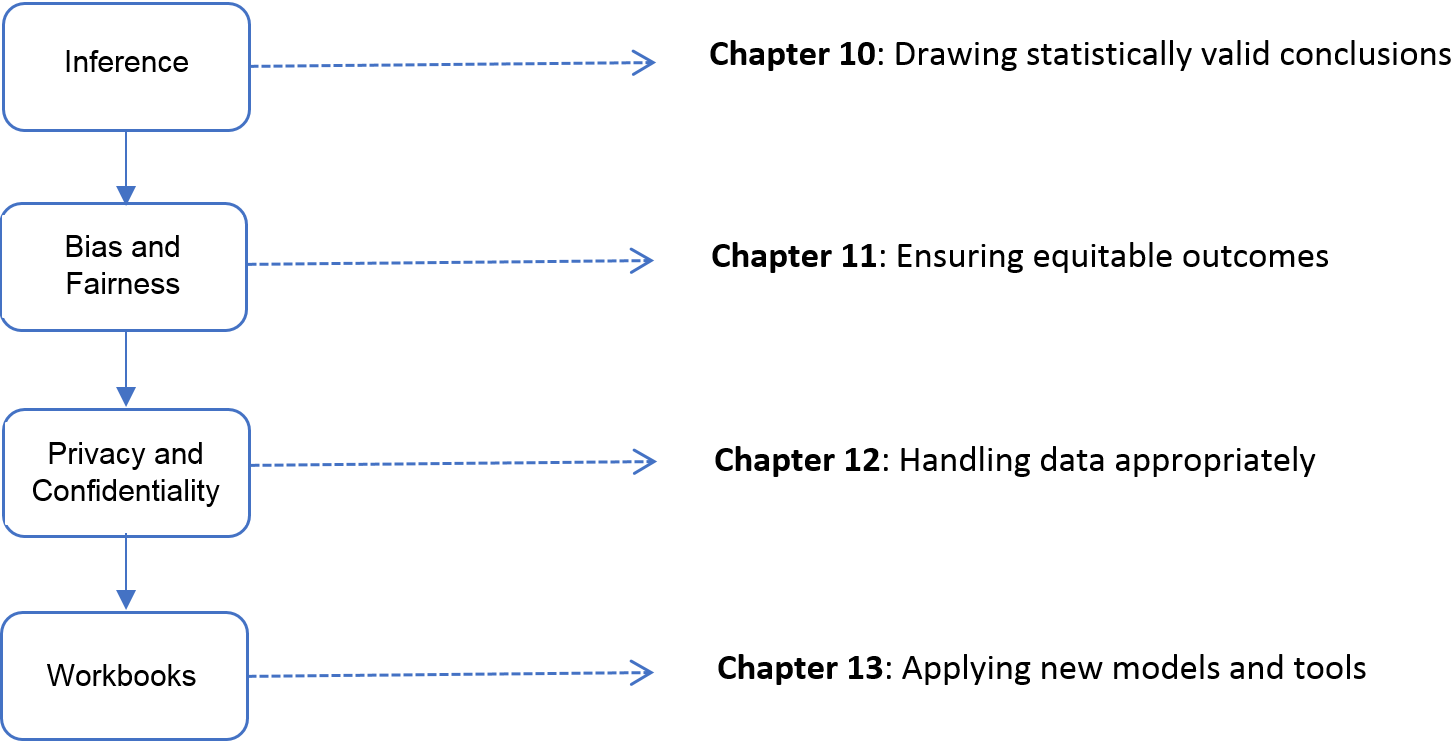
\includegraphics[width=0.9\linewidth]{ChapterIntro/figures/Figure4_new} 

}

\caption{The four chapters in Part III focus on *inference* and *ethics*}\label{fig:fig5}
\end{figure}

\section{Resources}\label{sec:intro:resources}

For more information on the \textbf{science of science policy}, see
Husbands et al.'s book for a full discussion of many issues (Husband
Fealing et al. \protect\hyperlink{ref-husband2011science}{2011}) and
peruse the awards made by the National Science Foundation's Science of
Science: Discovery, Communication, and Impact program
(\url{https://www.nsf.gov/funding/pgm_summ.jsp?pims_id=505730}).

This book is above all a \emph{practical} introduction to the methods
and tools that the social scientist can use to make sense of big data,
and thus \textbf{programming} resources are also important. We make
extensive use of the Python programming language and databases in both
the book and its supporting workbooks. We recommend that any social
scientist who aspires to work with large data sets become proficient in
the use of these two systems and GitHub. All three, fortunately, are
quite accessible and are supported by excellent online resources. Time
spent mastering them will be repaid many times over in more productive
research.

For \textbf{Python}\footnote{Read this!
  \url{http://alexbell.net/pyseminar/pyseminar.html}}, Alex Bell's
\emph{Python for Economists} (available online (Bell
\protect\hyperlink{ref-BellPython}{2012})) provides a wonderful 30-page
introduction to the use of Python in the social sciences, complete with
XKCD cartoons. Economists Tom Sargent and John Stachurski provide a very
useful set of lectures and examples at \url{http://quant-econ.net/}. For
more detail, we recommend Charles Severance's \emph{Python for
Informatics: Exploring Information} (Severance
\protect\hyperlink{ref-SeverancePython}{2013}), which not only covers
basic Python but also provides material relevant to web data (the
subject of \protect\hyperlink{chap:web}{Working with Web Data and APIs})
and MySQL (the subject of \protect\hyperlink{chap:db}{Databases}). This
book is also freely available online and is supported by excellent
online lectures and exercises.

For \textbf{SQL}, Chapter \protect\hyperlink{chap:db}{Databases}
provides introductory material and pointers to additional resources, so
we will not say more here.

We also recommend that you master \textbf{GitHub}. A version control
system is a tool for keeping track of changes that have been made to a
document over time. GitHub is a hosting service for projects that use
the Git version control system. As Strasser explains (Strasser
\protect\hyperlink{ref-GitResearch}{2014}), Git/GitHub makes it
straightforward for researchers to create digital lab notebooks that
record the data files, programs, papers, and other resources associated
with a project, with automatic tracking of the changes that are made to
those resources over time. GitHub also makes it easy for collaborators
to work together on a project, whether a program or a paper: changes
made by each contributor are recorded and can easily be reconciled. For
example, we used GitHub to create this book, with authors and editors
checking in changes and comments at different times and from many time
zones. We also use GitHub to provide access to the supporting workbooks.
Ram (Ram \protect\hyperlink{ref-ram2013git}{2013}) provides a nice
description of how Git/GitHub can be used to promote reproducibility and
transparency in research.

One more resource that is outside the scope of this book but that you
may well want to master is the \textbf{cloud} (Armbrust et al.
\protect\hyperlink{ref-armbrust2010view}{2010}; Lifka et al.
\protect\hyperlink{ref-Lifka}{2013}). It used to be that when your data
and computations became too large to analyze on your laptop, you were
out of luck unless your employer (or a friend) had a larger computer.
With the emergence of cloud storage and computing services from the
likes of Amazon Web Services, Google, and Microsoft, powerful computers
are available to anyone with a credit card. We and many others have had
positive experiences using such systems for the analysis of urban
(Catlett et al. \protect\hyperlink{ref-plenario}{2014}), environmental
(Elliott et al. \protect\hyperlink{ref-elliott2014parallel}{2014}), and
genomic (Bhuvaneshwar et al.
\protect\hyperlink{ref-bhuvaneshwar2015case}{2015}) data analysis and
modeling, for example.

\hypertarget{chap:web}{\chapter{Working with Web Data and
APIs}\label{chap:web}}

\textbf{Cameron Neylon}

In many social science problems we have to augment our primary data with
external data sources. Often the external data are available on the web,
either on web pages directly or accessible through Application
Programming Interfaces (APIs). Gathering this data requires
understanding how to scrape web pages or calling the APIs with
parameters about the information we need. One common example of this is
augmenting our primary data with data from the American Community Survey
(ACS) or from Open Data Portals maintained by local, state, and federal
agencies. These data sources can either be downloaded in bulk or used
dynamically through APIs. Same is true for data from social media
sources, such as Twitter, Instagram, and Facebook. In this chapter we
will cover tools (specifically using Python) that can be used by social
science researchers to programmatically gather this type of external
data from web pages and APIs.

\section{Introduction}\label{introduction}

The Internet is an excllent resource for vast amounts of data on
businesses, people, and their activity on social media. But how can we
capture the information and make use of it as we might make use of more
traditional data sources?

In social science, we often explore information on people,
organizations, or locations. The web can be a rich source of additional
information when doing this type of analysis, pointing to new sources of
information, allowing a pivot from one perspective to another, or from
one kind of query to another. Sometimes this data from the web is
completely unstructured, existing in web pages spread across a site, and
sometimes they are provided in a machine-readable form. In order to deal
with this variety, we need a sufficiently diverse toolkit to bring all
of this information together.\footnote{The chapter
  \protect\hyperlink{chap:privacy}{Privacy and Confidentiality} will
  discuss ethical issues when dealing with and using ``publically''
  available data for research and policy purposes.}

Using the example of data on researchers and research outputs, we will
focus this chapter on obtaining information directly from web pages
(\emph{web scraping}) as well as explore the uses of APIs---web services
that allow programmatic retrieval of data. Both in this chapter and the
next, you will see how the crucial pieces of integration often lie in
making connections between disparate data sets and how in turn making
those connections requires careful quality control. The emphasis
throughout this chapter is on the importance of focusing on the purpose
for which the data will be used as a guide for data collection. While
much of this is specific to data about research and researchers, the
ideas are generalizable to wider issues of data and public policy. While
we use Python as the programming language in this chapter, data
collection through web scraping and APIs can be done in most modern
programming languages as well as using software that's designed
specifically for this purpose.

\begin{center}\rule{0.5\linewidth}{\linethickness}\end{center}

\textbf{Box: Examples}

In addition to the worked examples in this chapter here are a few other
papers that show the wide variety of projects using data from web pages
or APIs.\footnote{If you have examples from your own research using the
  methods we describe in this chapter, please submit a link to the paper
  (and/or code) here:
  \url{https://textbook.coleridgeinitiative.org/submitexamples}}

Kim et al. (\protect\hyperlink{ref-Kim2016}{2016}) use social media data
about e-cigarettes from Twitter for public health research.

Goebel and Munzert (\protect\hyperlink{ref-Goebel2018}{2018}) used the
online encyclopedia Wikipedia, to study how politicians enhance and
change their appearance overtime. They trace changes to biographies
coming from the parliament using data that cover the entire edit
histories for biographies on all German members of parliament for the
three last legislative periods. The authors have workshop material and
code on GitHub how they performed the webscraping and API use for this
project
(\url{https://github.com/simonmunzert/political-wikipedia-workshop}).

King et al. (\protect\hyperlink{ref-King2013}{2013}) investigate how
censorship in China allows government criticism but silences collective
expression using a system to locate, download, and analyze the content
of millions of social media posts originating from nearly 1,400
different social media services all over China before the Chinese
government is able to find, evaluate, and censor (i.e., remove from the
Internet) the subset they deem objectionable.

\begin{center}\rule{0.5\linewidth}{\linethickness}\end{center}

\section{Scraping information from the
web}\label{scraping-information-from-the-web}

With the range of information available on the web, our first task is to
learn how to access it. The simplest approach is often to manually go to
the web and look for data files or other information. For instance, on
the NSF website\footnote{\url{https://nsf.gov/awardsearch/download.jsp}}
it is possible to obtain data downloads of all grant information.
Sometimes data are available through web pages or we only want a subset
of this information. In this case web scraping is often a viable
approach.

Web scraping involves writing code to download and process web pages
programmatically. We need to look at the website, identify how to get
the information we want from it, and then write code to do it. Many
websites deliberately make this difficult to prevent easy access to
their underlying data while some websites explicitly prohibit this type
of activity in their terms of use. Another challenge when scraping data
from websites is that the structure of the websites changes often,
requiring researchers to keep updating their code. This is also
important to note when using the code in this chapter. While the code
accurately captures the data from the website at the time of this
writing, it may not be valid in the future as the structure and content
of the website changes.

\subsection{Obtaining data from
websites}\label{obtaining-data-from-websites}

Let us suppose we are interested in obtaining information on those
investigators that are funded by the Howard Hughes Medical Institute
(HHMI). HHMI has a website that includes a search function for funded
researchers, including the ability to filter by field, state, and role.
But there does not appear to be a downloadable data set of this
information. However, we can automate the process with code to create a
data set that you might compare with other data.

\url{https://www.hhmi.org/scientists/browse?sort_by=field_scientist_last_name\&sort_order=ASC\&items_per_page=24}

Getting information from this web page programmatically requires us to
follow the following steps: 1. Constructing a URL that will give us the
results we want 2. Getting the contents of the page using that URL 3.
Processing the html response to extract the pieces of information we are
looking for (such as names and specialties of the scientists)

** Constructing the URL **

This process involves first understanding how to construct a URL that
will do the search we want. This is most easily done by playing with
search functionality and investigating the URL structures that are
returned.

With HHMI, if we do a general search and play with the structure of the
URL, we can see some of the elements of the URL that we can think of as
a query. As we want to see \emph{all} investigators, we do not need to
limit the search, and so with some fiddling we come up with a URL like
the following. (We have broken the one-line URL into three lines for
ease of presentation.)

\url{http://www.hhmi.org/scientists/browse?kw}=\&sort\_by=field\_scientist\_last\_name\&sort\_order=ASC\&items\_per\_page=24\&page=0

We can click on different links on the page modify part of this URL to
see how the search results change. For example, if we click on Sort by
Institution, the URL changes to

\url{https://www.hhmi.org/scientists/browse?sort_by=field_scientist_academic_institu\&sort_order=ASC\&items_per_page=24\&page=0}

If we click on next at the bottom, the url changes to
\url{https://www.hhmi.org/scientists/browse?sort_by=field_scientist_academic_institu\&sort_order=ASC\&items_per_page=24\&page=1}

This allows us to see that the URL is constructed using a few
parameters, such as sort\_by, sort\_order, items\_per\_page, and page
that can be programmatically modified to give us the search results that
we want.

\textbf{Getting the contents of the page from the URL}

The \texttt{requests} module, available natively in Jupyter Python
notebooks, is a useful set of tools for handling interactions with
websites. It lets us construct the request that we just presented in
terms of a base URL and query terms, as follows:

\begin{Shaded}
\begin{Highlighting}[]
\OperatorTok{>}\ErrorTok{>}\StringTok{ }\NormalTok{BASE_URL =}\StringTok{ "http://www.hhmi.org/scientists/browse"}
\OperatorTok{>}\ErrorTok{>}\StringTok{ }\NormalTok{query =}\StringTok{ }\NormalTok{\{}
            \StringTok{"kw"} \OperatorTok{:}\StringTok{ ""}\NormalTok{,}
            \StringTok{"sort_by"} \OperatorTok{:}\StringTok{ "field_scientist_last_name"}\NormalTok{,}
            \StringTok{"sort_order"} \OperatorTok{:}\StringTok{ "ASC"}\NormalTok{,}
            \StringTok{"items_per_page"} \OperatorTok{:}\StringTok{ }\DecValTok{24}\NormalTok{,}
            \StringTok{"page"} \OperatorTok{:}\StringTok{ }\NormalTok{None}
\NormalTok{           \}}
\end{Highlighting}
\end{Shaded}

With our request constructed we can then make the call to the web page
to get a response.

\begin{Shaded}
\begin{Highlighting}[]
\OperatorTok{>}\ErrorTok{>}\StringTok{ }\NormalTok{import requests}
\OperatorTok{>}\ErrorTok{>}\StringTok{ }\NormalTok{response =}\StringTok{ }\KeywordTok{requests.get}\NormalTok{(BASE_URL, }\DataTypeTok{params=}\NormalTok{query)}
\end{Highlighting}
\end{Shaded}

The first thing to do when building a script that hits a web page is to
make sure that your call was successful. This can be checked by looking
at the response code that the web server sent---and, obviously, by
checking the actual HTML that was returned. A \texttt{200} code means
success and that everything should be OK. Other codes may mean that the
URL was constructed wrongly or that there was a server error.

\begin{Shaded}
\begin{Highlighting}[]
\OperatorTok{>}\ErrorTok{>}\StringTok{ }\NormalTok{response.status_code}
\DecValTok{200}
\end{Highlighting}
\end{Shaded}

\textbf{Processing the html response}

With the page successfully returned, we now need to process the text it
contains into the data we want. This is not a trivial exercise. Web
pages are typically written in a ``markup'' language called Hyptertext
Markup Language (HTML). This language tells the web browser how to
display the content on that web page such as making a piece of text bold
or in italics, creating numbered lists, or showing images. When we use
Python to retrieve a webpage, running the code gives us the HTML text.
We then have to process this text to extract the content that we care
about. There are a range of tools in Python that can help with
processing HTML data. One of the most popular is a module BeautifulSoup
(Richardson, n.d.), which provides a number of useful functions for this
kind of processing. The module documentation provides more details.

We need to check the details of the page source to find where the
information we are looking for is kept (see, for example, Figure
\ref{fig:fig2-1}). Here, all the details on HHMI investigators can be
found in a \texttt{\textless{}div\textgreater{}} element with the class
attribute \texttt{view-content}. This structure is not something that
can be determined in advance. It requires knowledge of the structure of
the page itself. Nested inside this
\texttt{\textless{}div\textgreater{}} element are another series of
\texttt{div}s, each of which corresponds to one investigator. These have
the class attribute \texttt{view-rows}. Again, there is nothing obvious
about finding these, it requires a close examination of the page HTML
itself for any specific case you happen to be looking at.

\begin{figure}

{\centering 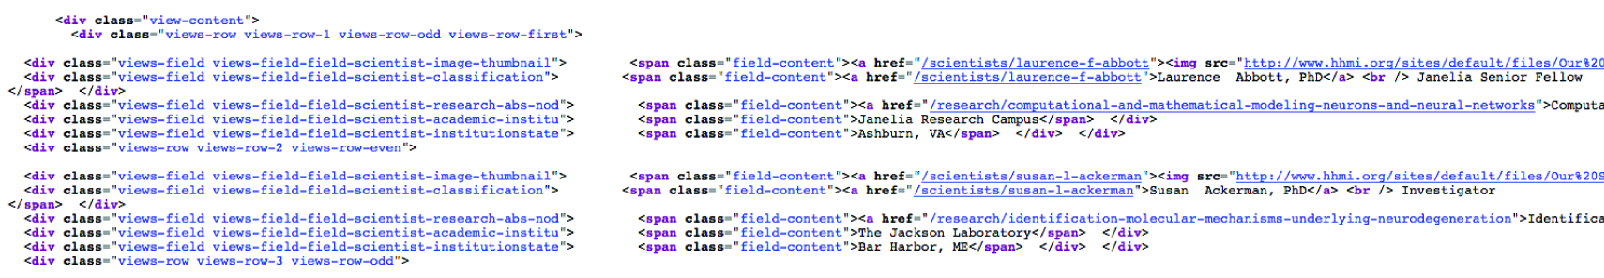
\includegraphics[width=0.9\linewidth]{ChapterWeb/figures/fig2-1} 

}

\caption{Source HTML from the portion of an HHMI results page containing information on HHMI investigators; note that the webscraping results in badly formatted html which is difficult to read.}\label{fig:fig2-1}
\end{figure}

We first process the page using the BeautifulSoup module (into the
variable \texttt{soup}) and then find the \texttt{div} element that
holds the information on investigators (\texttt{investigator\_list}). As
this element is unique on the page (I checked using my web browser), we
can use the find method. We then process that \texttt{div} (using
\texttt{find\_all}) to create an iterator object that contains each of
the page segments detailing a single investigator
(\texttt{investigators}).

\begin{Shaded}
\begin{Highlighting}[]
\OperatorTok{>}\ErrorTok{>}\StringTok{ }\NormalTok{from bs4 import BeautifulSoup}
\OperatorTok{>}\ErrorTok{>}\StringTok{ }\NormalTok{soup =}\StringTok{ }\KeywordTok{BeautifulSoup}\NormalTok{(response.text, }\StringTok{"html5lib"}\NormalTok{)}
\OperatorTok{>}\ErrorTok{>}\StringTok{ }\NormalTok{investigator_list =}\StringTok{ }\KeywordTok{soup.find}\NormalTok{(}\StringTok{'div'}\NormalTok{, }\DataTypeTok{class_ =} \StringTok{"view-content"}\NormalTok{)}
\OperatorTok{>}\ErrorTok{>}\StringTok{ }\NormalTok{investigators =}\StringTok{ }\KeywordTok{investigator_list.find_all}\NormalTok{(}\StringTok{"div"}\NormalTok{, }\DataTypeTok{class_ =} \StringTok{"views-row"}\NormalTok{)}
\end{Highlighting}
\end{Shaded}

As we specified in our query parameters that we wanted 24 results per
page, we should check whether our list of page sections has the right
length.

\begin{Shaded}
\begin{Highlighting}[]
\OperatorTok{>}\ErrorTok{>}\StringTok{ }\KeywordTok{len}\NormalTok{(investigators)}
\DecValTok{20}
\end{Highlighting}
\end{Shaded}

\begin{Shaded}
\begin{Highlighting}[]
\CommentTok{# Given a request response object, parse for HHMI investigators}
\NormalTok{def }\KeywordTok{scrape}\NormalTok{(page_response)}\OperatorTok{:}
\StringTok{   }\CommentTok{# Obtain response HTML and the correct <div> from the page}
\StringTok{   }\NormalTok{soup =}\StringTok{ }\KeywordTok{BeautifulSoup}\NormalTok{(response.text, }\StringTok{"html5lib"}\NormalTok{)}
\NormalTok{   inv_list =}\StringTok{ }\KeywordTok{soup.find}\NormalTok{(}\StringTok{'div'}\NormalTok{, }\DataTypeTok{class_ =} \StringTok{"view-content"}\NormalTok{)}

   \CommentTok{# Create a list of all the investigators on the page}
\NormalTok{   investigators =}\StringTok{ }\KeywordTok{inv_list.find_all}\NormalTok{(}\StringTok{"div"}\NormalTok{, }\DataTypeTok{class_ =} \StringTok{"views-row"}\NormalTok{)}

\NormalTok{   data =}\StringTok{ }\NormalTok{[] }\CommentTok{# Make the data object to store scraping results}

   \CommentTok{# Scrape needed elements from investigator list}
   \ControlFlowTok{for}\NormalTok{ investigator }\ControlFlowTok{in}\NormalTok{ investigators}\OperatorTok{:}
\StringTok{       }\NormalTok{inv =}\StringTok{ }\NormalTok{\{\} }\CommentTok{# Create a dictionary to store results}

       \CommentTok{# Name and role are in same HTML element; this code}
       \CommentTok{# separates them into two data elements}
\NormalTok{       name_role_tag =}\StringTok{ }\KeywordTok{investigator.find}\NormalTok{(}\StringTok{"div"}\NormalTok{,}
           \DataTypeTok{class_ =} \StringTok{"views-field-field-scientist-classification"}\NormalTok{)}
\NormalTok{       strings =}\StringTok{ }\NormalTok{name_role_tag.stripped_strings}
       \ControlFlowTok{for}\NormalTok{ string,a }\ControlFlowTok{in} \KeywordTok{zip}\NormalTok{(strings, [}\StringTok{"name"}\NormalTok{, }\StringTok{"role"}\NormalTok{])}\OperatorTok{:}
\StringTok{           }\NormalTok{inv[a] =}\StringTok{ }\NormalTok{string}

       \CommentTok{# Extract other elements from text of specific divs or from}
       \CommentTok{# class attributes of tags in the page (e.g., URLs)}
\NormalTok{       research_tag =}\StringTok{ }\KeywordTok{investigator.find}\NormalTok{(}\StringTok{"div"}\NormalTok{,}
          \DataTypeTok{class_ =} \StringTok{"views-field-field-scientist-research-abs-nod"}\NormalTok{)}
\NormalTok{       inv[}\StringTok{"research"}\NormalTok{] =}\StringTok{ }\KeywordTok{research_tag.text.lstrip}\NormalTok{()}
\NormalTok{       inv[}\StringTok{"research_url"}\NormalTok{] =}\StringTok{ "http://hhmi.org"}
          \OperatorTok{+}\StringTok{ }\KeywordTok{research_tag.find}\NormalTok{(}\StringTok{"a"}\NormalTok{)}\KeywordTok{.get}\NormalTok{(}\StringTok{"href"}\NormalTok{)}
\NormalTok{       institution_tag =}\StringTok{ }\KeywordTok{investigator.find}\NormalTok{(}\StringTok{"div"}\NormalTok{,}
          \DataTypeTok{class_ =} \StringTok{"views-field-field-scientist-academic-institu"}\NormalTok{)}
\NormalTok{       inv[}\StringTok{"institute"}\NormalTok{] =}\StringTok{ }\KeywordTok{institution_tag.text.lstrip}\NormalTok{()}
\NormalTok{       town_state_tag =}\StringTok{ }\KeywordTok{investigator.find}\NormalTok{(}\StringTok{"div"}\NormalTok{,}
           \DataTypeTok{class_ =} \StringTok{"views-field-field-scientist-institutionstate"}\NormalTok{)}
\NormalTok{       inv[}\StringTok{"town"}\NormalTok{], inv[}\StringTok{"state"}\NormalTok{] =}\StringTok{ }\KeywordTok{town_state_tag.text.split}\NormalTok{(}\StringTok{","}\NormalTok{)}
\NormalTok{       inv[}\StringTok{"town"}\NormalTok{] =}\StringTok{ }\KeywordTok{inv.get}\NormalTok{(}\StringTok{"town"}\NormalTok{)}\KeywordTok{.lstrip}\NormalTok{()}
\NormalTok{       inv[}\StringTok{"state"}\NormalTok{] =}\StringTok{ }\KeywordTok{inv.get}\NormalTok{(}\StringTok{"state"}\NormalTok{)}\KeywordTok{.lstrip}\NormalTok{()}

\NormalTok{       thumbnail_tag =}\StringTok{ }\KeywordTok{investigator.find}\NormalTok{(}\StringTok{"div"}\NormalTok{,}
          \DataTypeTok{class_ =} \StringTok{"views-field-field-scientist-image-thumbnail"}\NormalTok{)}
\NormalTok{       inv[}\StringTok{"thumbnail_url"}\NormalTok{] =}\StringTok{ }\KeywordTok{thumbnail_tag.find}\NormalTok{(}\StringTok{"img"}\NormalTok{)[}\StringTok{"src"}\NormalTok{]}
\NormalTok{       inv[}\StringTok{"url"}\NormalTok{] =}\StringTok{ "http://hhmi.org"}
          \OperatorTok{+}\StringTok{ }\KeywordTok{thumbnail_tag.find}\NormalTok{(}\StringTok{"a"}\NormalTok{)}\KeywordTok{.get}\NormalTok{(}\StringTok{"href"}\NormalTok{)}

       \CommentTok{# Add the new data to the list}
       \KeywordTok{data.append}\NormalTok{(inv)}
\NormalTok{   return data}
\end{Highlighting}
\end{Shaded}

Listing 2.1. Python code to parse for HHMI investigators

Finally, we need to process each of these segments to obtain the data we
are looking for. This is the actual ``scraping'' of the page to get the
information we want. Again, this involves looking closely at the HTML
itself, identifying where the information is held, what tags can be used
to find it, and often doing some post-processing to clean it up
(removing spaces, splitting different elements up, etc.).

Listing \protect\hyperlink{list:web1}{Investigators} provides a function
to handle all of this. The function accepts the response object from the
requests module as its input, processes the page text to soup, and then
finds the \texttt{investigator\_list} as above and processes it into an
actual list of the investigators. For each investigator it then
processes the HTML to find and clean up the information required,
converting it to a dictionary and adding it to our growing list of data.

Let us check what the first two elements of our data set now look like.
You can see two dictionaries, one relating to Laurence Abbott, who is a
senior fellow at the HHMI Janelia Farm Campus, and one for Susan
Ackerman, an HHMI investigator based at the Jackson Laboratory in Bar
Harbor, Maine. Note that we have also obtained URLs that give more
details on the researcher and their research program
(\texttt{research\_url} and \texttt{url} keys in the dictionary) that
could provide a useful input to textual analysis or topic modeling (see
Chapter \protect\hyperlink{chap:text}{Text Analysis}).

\begin{Shaded}
\begin{Highlighting}[]
\OperatorTok{>}\ErrorTok{>}\StringTok{ }\NormalTok{data =}\StringTok{ }\KeywordTok{scrape}\NormalTok{(response)}
\OperatorTok{>}\ErrorTok{>}\StringTok{ }\NormalTok{data[}\DecValTok{0}\OperatorTok{:}\DecValTok{2}\NormalTok{]}
\NormalTok{[\{}\StringTok{'institute'}\OperatorTok{:}\StringTok{ }\NormalTok{u}\StringTok{'Janelia Research Campus '}\NormalTok{,}
  \StringTok{'name'}\OperatorTok{:}\StringTok{ }\NormalTok{u}\StringTok{'Laurence Abbott, PhD'}\NormalTok{,}
  \StringTok{'research'}\OperatorTok{:}\StringTok{ }\NormalTok{u}\StringTok{'Computational and Mathematical Modeling of Neurons and Neural... '}\NormalTok{,}
  \StringTok{'research_url'}\OperatorTok{:}\StringTok{ }\NormalTok{u}\StringTok{'http://hhmi.org/research/computational-and-mathematical-modeling-neurons-and-neural-networks'}\NormalTok{,}
  \StringTok{'role'}\OperatorTok{:}\StringTok{ }\NormalTok{u}\StringTok{'Janelia Senior Fellow'}\NormalTok{,}
  \StringTok{'state'}\OperatorTok{:}\StringTok{ }\NormalTok{u}\StringTok{'VA '}\NormalTok{,}
  \StringTok{'thumbnail_url'}\OperatorTok{:}\StringTok{ }\NormalTok{u}\StringTok{'http://www.hhmi.org/sites/default/files/Our%20Scientists/Janelia/Abbott-112x112.jpg'}\NormalTok{,}
  \StringTok{'town'}\OperatorTok{:}\StringTok{ }\NormalTok{u}\StringTok{'Ashburn'}\NormalTok{,}
  \StringTok{'url'}\OperatorTok{:}\StringTok{ }\NormalTok{u}\StringTok{'http://hhmi.org/scientists/laurence-f-abbott'}\NormalTok{\},}
\NormalTok{ \{}\StringTok{'institute'}\OperatorTok{:}\StringTok{ }\NormalTok{u}\StringTok{'The Jackson Laboratory '}\NormalTok{,}
  \StringTok{'name'}\OperatorTok{:}\StringTok{ }\NormalTok{u}\StringTok{'Susan Ackerman, PhD'}\NormalTok{,}
  \StringTok{'research'}\OperatorTok{:}\StringTok{ }\NormalTok{u}\StringTok{'Identification of the Molecular Mechanisms Underlying... '}\NormalTok{,}
  \StringTok{'research_url'}\OperatorTok{:}\StringTok{ }\NormalTok{u}\StringTok{'http://hhmi.org/research/identification-molecular-mechanisms-underlying-neurodegeneration'}\NormalTok{,}
  \StringTok{'role'}\OperatorTok{:}\StringTok{ }\NormalTok{u}\StringTok{'Investigator'}\NormalTok{,}
  \StringTok{'state'}\OperatorTok{:}\StringTok{ }\NormalTok{u}\StringTok{'ME '}\NormalTok{,}
  \StringTok{'thumbnail_url'}\OperatorTok{:}
\NormalTok{u}\StringTok{'http://www.hhmi.org/sites/default/files/Our%20Scientists/Investigators/Ackerman-112x112.jpg'}\NormalTok{,}
  \StringTok{'town'}\OperatorTok{:}\StringTok{ }\NormalTok{u}\StringTok{'Bar Harbor'}\NormalTok{,}
  \StringTok{'url'}\OperatorTok{:}\StringTok{ }\NormalTok{u}\StringTok{'http://hhmi.org/scientists/susan-l-ackerman'}\NormalTok{\}]}
\end{Highlighting}
\end{Shaded}

** Programmatically Iterating over the Search Results **

Now we know we can process a page from a website to generate useful
structured data. However, this was only the first page of results. We
need to do this for each page of results if we want to capture all the
HHMI investigators. We could just look at the number of pages that our
search returned manually, but to make this more general we can actually
scrape the page to find that piece of information and use that to
calculate how many pages we need to iterate through.

The number of results is found in a \texttt{div} with the class
``view-headers'' as a piece of free text (``Showing 1--20 of 493
results''). We need to grab the text, split it up (we do so based on
spaces), find the right number (the one that is before the word
``results'') and convert that to an integer. Then we can divide by the
number of items we requested per page (20 in our case) to find how many
pages we need to work through. A quick mental calculation confirms that
if page 0 had results 1--20, page 24 would give results 481--493.

\begin{Shaded}
\begin{Highlighting}[]
\OperatorTok{>}\ErrorTok{>}\StringTok{ }\CommentTok{# Check total number of investigators returned}
\ErrorTok{>>}\StringTok{ }\NormalTok{view_header =}\StringTok{ }\KeywordTok{soup.find}\NormalTok{(}\StringTok{"div"}\NormalTok{, }\DataTypeTok{class_ =} \StringTok{"view-header"}\NormalTok{)}
\OperatorTok{>}\ErrorTok{>}\StringTok{ }\NormalTok{words =}\StringTok{ }\KeywordTok{view_header.text.split}\NormalTok{(}\StringTok{" "}\NormalTok{)}
\OperatorTok{>}\ErrorTok{>}\StringTok{ }\NormalTok{count_index =}\StringTok{ }\KeywordTok{words.index}\NormalTok{(}\StringTok{"results."}\NormalTok{) }\OperatorTok{-}\StringTok{ }\DecValTok{1}
\OperatorTok{>}\ErrorTok{>}\StringTok{ }\NormalTok{count =}\StringTok{ }\KeywordTok{int}\NormalTok{(words[count_index])}

\OperatorTok{>}\ErrorTok{>}\StringTok{ }\CommentTok{# Calculate number of pages, given count & items_per_page}
\ErrorTok{>>}\StringTok{ }\NormalTok{num_pages =}\StringTok{ }\NormalTok{count}\OperatorTok{/}\KeywordTok{query.get}\NormalTok{(}\StringTok{"items_per_page"}\NormalTok{)}
\OperatorTok{>}\ErrorTok{>}\StringTok{ }\NormalTok{num_pages}
\DecValTok{24}
\end{Highlighting}
\end{Shaded}

Then it is a matter of putting the function we constructed earlier into
a loop to work through the correct number of pages. As we start to hit
the website repeatedly, we need to consider whether we are being polite.
Most websites have a file in the root directory called robots.txt that
contains guidance on using programs to interact with the website. In the
case of \url{http://hhmi.org} the file states first that we are allowed
(or, more properly, not forbidden) to query
\url{http://www.hhmi.org/scientists/} programmatically. Thus, you can
pull down all of the more detailed biographical or research information,
if you so desire. The file also states that there is a requested
``Crawl-delay'' of 10. This means that if you are making repeated
queries (as we will be in getting the 24 pages), you should wait for 10
seconds between each query. This request is easily accommodated by
adding a timed delay between each page request.

\begin{Shaded}
\begin{Highlighting}[]
\OperatorTok{>}\ErrorTok{>}\StringTok{ }\ControlFlowTok{for}\NormalTok{ page_num }\ControlFlowTok{in} \KeywordTok{range}\NormalTok{(num_pages)}\OperatorTok{:}
\ErrorTok{>>}\StringTok{ }\CommentTok{# We already have page zero and we need to go to 24:}
\ErrorTok{>>}\StringTok{ }\CommentTok{# range(24) is [0,1,...,23]}
\ErrorTok{>>}\StringTok{    }\NormalTok{query[}\StringTok{"items_per_page"}\NormalTok{] =}\StringTok{ }\NormalTok{page_num }\OperatorTok{+}\StringTok{ }\DecValTok{1}
\OperatorTok{>}\ErrorTok{>}\StringTok{    }\NormalTok{page =}\StringTok{ }\KeywordTok{requests.get}\NormalTok{(BASE_URL, }\DataTypeTok{params=}\NormalTok{query)}
\OperatorTok{>}\ErrorTok{>}\StringTok{ }\CommentTok{# We use extend to add list for each page to existing list}
\ErrorTok{>>}\StringTok{    }\KeywordTok{data.extend}\NormalTok{(}\KeywordTok{scrape}\NormalTok{(page))}
\OperatorTok{>}\ErrorTok{>}\StringTok{ }\KeywordTok{print}\NormalTok{(}\StringTok{"Retrieved and scraped page number:"}\NormalTok{, }\KeywordTok{query.get}\NormalTok{(}\StringTok{"items_per_page"}\NormalTok{))}
\OperatorTok{>}\ErrorTok{>}\StringTok{ }\KeywordTok{time.sleep}\NormalTok{(}\DecValTok{10}\NormalTok{) }\CommentTok{# robots.txt at hhmi.org specifies a crawl delay of 10 seconds}
\NormalTok{Retrieved and scraped page number}\OperatorTok{:}\StringTok{ }\DecValTok{1}
\NormalTok{Retrieved and scraped page number}\OperatorTok{:}\StringTok{ }\DecValTok{2}
\NormalTok{...}
\NormalTok{Retrieved and scraped page number}\OperatorTok{:}\StringTok{ }\DecValTok{24}
\end{Highlighting}
\end{Shaded}

Finally we can check that we have the right number of results after our
scraping. This should correspond to the 493 records that the website
reports.

\begin{Shaded}
\begin{Highlighting}[]
\OperatorTok{>}\ErrorTok{>}\StringTok{ }\KeywordTok{len}\NormalTok{(data)}
\DecValTok{493}
\end{Highlighting}
\end{Shaded}

\subsection{Limits of scraping}\label{limits-of-scraping}

While scraping websites is often necessary, is can be a fragile and
messy way of working. It is problematic for a number of reasons: for
example, many websites are designed in ways that make scraping difficult
or impossible, and other sites explicitly prohibit this kind of scripted
analysis. (Both reasons apply in the case of the NSF and Grants.gov
websites, which is why we use the HHMI website in our example.) The
structure of websites also changes frequently, forcing you to
continuously modify your code to keep up with the structure.

In many cases a better choice is to process a data download from an
organization. For example, the NSF and Wellcome Trust both provide data
sets for each year that include structured data on all their awarded
grants. In practice, integrating data is a continual challenge of
figuring out what is the easiest way to proceed, what is allowed, and
what is practical and useful. The selection of data will often be driven
by pragmatic rather than theoretical concerns.

Increasingly, organizations are providing APIs to enable scripted and
programmatic access to the data they hold. These tools are much easier
and generally more effective to work with. They are the focus of much of
the rest of this chapter.

\section{Application Programming Interfaces
(APIs)}\label{application-programming-interfaces-apis}

An API is simply a tool that allows a program to interface with a
service. APIs can take many different forms and be of varying quality
and usefulness. In this section we will focus on one common type of API
and examples of important publicly available APIs relevant to research
communications. We will also cover combining APIs and the benefits and
challenges of bringing multiple data sources together.

\subsection{Relevant APIs and
resources}\label{relevant-apis-and-resources}

There is a wide range of other sources of information that can be used
in combination with the APIs featured above to develop an overview of
research outputs and of where and how they are being used. There are
also other tools that can allow deeper analysis of the outputs
themselves. Table \ref{tab:table2-1} gives a partial list of key data
sources and APIs that are relevant to the analysis of research outputs.

\begin{longtable}[]{@{}llcc@{}}
\caption{\label{tab:table2-1} Popular sources of data relevant to the
analysis of research outputs}\tabularnewline
\toprule
\begin{minipage}[b]{0.10\columnwidth}\raggedright\strut
\textbf{Source}\strut
\end{minipage} & \begin{minipage}[b]{0.74\columnwidth}\raggedright\strut
\textbf{Description}\strut
\end{minipage} & \begin{minipage}[b]{0.02\columnwidth}\centering\strut
\textbf{API}\strut
\end{minipage} & \begin{minipage}[b]{0.02\columnwidth}\centering\strut
\textbf{Free}\strut
\end{minipage}\tabularnewline
\midrule
\endfirsthead
\toprule
\begin{minipage}[b]{0.10\columnwidth}\raggedright\strut
\textbf{Source}\strut
\end{minipage} & \begin{minipage}[b]{0.74\columnwidth}\raggedright\strut
\textbf{Description}\strut
\end{minipage} & \begin{minipage}[b]{0.02\columnwidth}\centering\strut
\textbf{API}\strut
\end{minipage} & \begin{minipage}[b]{0.02\columnwidth}\centering\strut
\textbf{Free}\strut
\end{minipage}\tabularnewline
\midrule
\endhead
\begin{minipage}[t]{0.10\columnwidth}\raggedright\strut
\strut
\end{minipage} & \begin{minipage}[t]{0.74\columnwidth}\raggedright\strut
\textbf{Bibliographic Data}\strut
\end{minipage} & \begin{minipage}[t]{0.02\columnwidth}\centering\strut
\strut
\end{minipage} & \begin{minipage}[t]{0.02\columnwidth}\centering\strut
\strut
\end{minipage}\tabularnewline
\begin{minipage}[t]{0.10\columnwidth}\raggedright\strut
PubMed\strut
\end{minipage} & \begin{minipage}[t]{0.74\columnwidth}\raggedright\strut
An online index that combines bibliographic data from Medline and PubMed
Central. PubMed Central and Europe PubMed Central also provide
information.\strut
\end{minipage} & \begin{minipage}[t]{0.02\columnwidth}\centering\strut
Y\strut
\end{minipage} & \begin{minipage}[t]{0.02\columnwidth}\centering\strut
Y\strut
\end{minipage}\tabularnewline
\begin{minipage}[t]{0.10\columnwidth}\raggedright\strut
Web of Science\strut
\end{minipage} & \begin{minipage}[t]{0.74\columnwidth}\raggedright\strut
The bibliographic database provided by Thomson Reuters. The ISI Citation
Index is also available.\strut
\end{minipage} & \begin{minipage}[t]{0.02\columnwidth}\centering\strut
Y\strut
\end{minipage} & \begin{minipage}[t]{0.02\columnwidth}\centering\strut
N\strut
\end{minipage}\tabularnewline
\begin{minipage}[t]{0.10\columnwidth}\raggedright\strut
Scopus\strut
\end{minipage} & \begin{minipage}[t]{0.74\columnwidth}\raggedright\strut
The bibliographic database provided by Elsevier. It also provides
citation information.\strut
\end{minipage} & \begin{minipage}[t]{0.02\columnwidth}\centering\strut
Y\strut
\end{minipage} & \begin{minipage}[t]{0.02\columnwidth}\centering\strut
N\strut
\end{minipage}\tabularnewline
\begin{minipage}[t]{0.10\columnwidth}\raggedright\strut
Crossref\strut
\end{minipage} & \begin{minipage}[t]{0.74\columnwidth}\raggedright\strut
Provides a range of bibliographic metadata and information obtained from
members registering DOIs.\strut
\end{minipage} & \begin{minipage}[t]{0.02\columnwidth}\centering\strut
Y\strut
\end{minipage} & \begin{minipage}[t]{0.02\columnwidth}\centering\strut
Y\strut
\end{minipage}\tabularnewline
\begin{minipage}[t]{0.10\columnwidth}\raggedright\strut
Google Scholar\strut
\end{minipage} & \begin{minipage}[t]{0.74\columnwidth}\raggedright\strut
Provides a search index for scholarly objects and aggregates citation
information.\strut
\end{minipage} & \begin{minipage}[t]{0.02\columnwidth}\centering\strut
N\strut
\end{minipage} & \begin{minipage}[t]{0.02\columnwidth}\centering\strut
Y\strut
\end{minipage}\tabularnewline
\begin{minipage}[t]{0.10\columnwidth}\raggedright\strut
Microsoft Academic Search\strut
\end{minipage} & \begin{minipage}[t]{0.74\columnwidth}\raggedright\strut
Provides a search index for scholarly objects and aggregates citation
information. Not as complete as Google Scholar, but has an API.\strut
\end{minipage} & \begin{minipage}[t]{0.02\columnwidth}\centering\strut
Y\strut
\end{minipage} & \begin{minipage}[t]{0.02\columnwidth}\centering\strut
Y\strut
\end{minipage}\tabularnewline
\begin{minipage}[t]{0.10\columnwidth}\raggedright\strut
\strut
\end{minipage} & \begin{minipage}[t]{0.74\columnwidth}\raggedright\strut
\textbf{Social Media}\strut
\end{minipage} & \begin{minipage}[t]{0.02\columnwidth}\centering\strut
\strut
\end{minipage} & \begin{minipage}[t]{0.02\columnwidth}\centering\strut
\strut
\end{minipage}\tabularnewline
\begin{minipage}[t]{0.10\columnwidth}\raggedright\strut
Altmetric.com\strut
\end{minipage} & \begin{minipage}[t]{0.74\columnwidth}\raggedright\strut
A provider of aggregated data on social media and mainstream media
attention of research outputs. Most comprehensive source of information
across different social media and mainstream media conversations.\strut
\end{minipage} & \begin{minipage}[t]{0.02\columnwidth}\centering\strut
Y\strut
\end{minipage} & \begin{minipage}[t]{0.02\columnwidth}\centering\strut
N\strut
\end{minipage}\tabularnewline
\begin{minipage}[t]{0.10\columnwidth}\raggedright\strut
Twitter\strut
\end{minipage} & \begin{minipage}[t]{0.74\columnwidth}\raggedright\strut
Provides an API that allows a user to search for recent tweets and
obtain some information on specific accounts.\strut
\end{minipage} & \begin{minipage}[t]{0.02\columnwidth}\centering\strut
Y\strut
\end{minipage} & \begin{minipage}[t]{0.02\columnwidth}\centering\strut
Y\strut
\end{minipage}\tabularnewline
\begin{minipage}[t]{0.10\columnwidth}\raggedright\strut
Facebook\strut
\end{minipage} & \begin{minipage}[t]{0.74\columnwidth}\raggedright\strut
The Facebook API gives information on the number of pages, likes, and
posts associated with specific web pages\strut
\end{minipage} & \begin{minipage}[t]{0.02\columnwidth}\centering\strut
Y\strut
\end{minipage} & \begin{minipage}[t]{0.02\columnwidth}\centering\strut
Y\strut
\end{minipage}\tabularnewline
\begin{minipage}[t]{0.10\columnwidth}\raggedright\strut
\strut
\end{minipage} & \begin{minipage}[t]{0.74\columnwidth}\raggedright\strut
\textbf{Author Profiles}\strut
\end{minipage} & \begin{minipage}[t]{0.02\columnwidth}\centering\strut
\strut
\end{minipage} & \begin{minipage}[t]{0.02\columnwidth}\centering\strut
\strut
\end{minipage}\tabularnewline
\begin{minipage}[t]{0.10\columnwidth}\raggedright\strut
ORCID\strut
\end{minipage} & \begin{minipage}[t]{0.74\columnwidth}\raggedright\strut
Unique identifiers for research authors. Profiles include information on
publication lists, grants, and affiliations.\strut
\end{minipage} & \begin{minipage}[t]{0.02\columnwidth}\centering\strut
Y\strut
\end{minipage} & \begin{minipage}[t]{0.02\columnwidth}\centering\strut
Y\strut
\end{minipage}\tabularnewline
\begin{minipage}[t]{0.10\columnwidth}\raggedright\strut
LinkedIn\strut
\end{minipage} & \begin{minipage}[t]{0.74\columnwidth}\raggedright\strut
CV-based profiles, projects, and publications.\strut
\end{minipage} & \begin{minipage}[t]{0.02\columnwidth}\centering\strut
Y\strut
\end{minipage} & \begin{minipage}[t]{0.02\columnwidth}\centering\strut
*\strut
\end{minipage}\tabularnewline
\begin{minipage}[t]{0.10\columnwidth}\raggedright\strut
\strut
\end{minipage} & \begin{minipage}[t]{0.74\columnwidth}\raggedright\strut
\textbf{Funder Information}\strut
\end{minipage} & \begin{minipage}[t]{0.02\columnwidth}\centering\strut
\strut
\end{minipage} & \begin{minipage}[t]{0.02\columnwidth}\centering\strut
\strut
\end{minipage}\tabularnewline
\begin{minipage}[t]{0.10\columnwidth}\raggedright\strut
Gateway to Research\strut
\end{minipage} & \begin{minipage}[t]{0.74\columnwidth}\raggedright\strut
A database of funding decisions and related outputs from Research
Councils UK.\strut
\end{minipage} & \begin{minipage}[t]{0.02\columnwidth}\centering\strut
Y\strut
\end{minipage} & \begin{minipage}[t]{0.02\columnwidth}\centering\strut
Y\strut
\end{minipage}\tabularnewline
\begin{minipage}[t]{0.10\columnwidth}\raggedright\strut
NIH Reporter\strut
\end{minipage} & \begin{minipage}[t]{0.74\columnwidth}\raggedright\strut
Online search for information on National Institutes of Health grants.
Does not provide an API but a downloadable data set is available.\strut
\end{minipage} & \begin{minipage}[t]{0.02\columnwidth}\centering\strut
N\strut
\end{minipage} & \begin{minipage}[t]{0.02\columnwidth}\centering\strut
Y\strut
\end{minipage}\tabularnewline
\begin{minipage}[t]{0.10\columnwidth}\raggedright\strut
NSF Award Search\strut
\end{minipage} & \begin{minipage}[t]{0.74\columnwidth}\raggedright\strut
Online search for information on NSF grants. Does not provide an API but
downloadable data sets by year are available.\strut
\end{minipage} & \begin{minipage}[t]{0.02\columnwidth}\centering\strut
N\strut
\end{minipage} & \begin{minipage}[t]{0.02\columnwidth}\centering\strut
Y\strut
\end{minipage}\tabularnewline
\bottomrule
\end{longtable}

*The data are restricted: sometimes fee based, other times not.

\subsection{RESTful APIs, returned data, and Python
wrappers}\label{restful-apis-returned-data-and-python-wrappers}

The APIs we will focus on here are all examples of RESTful services.
REST stands for Representational State Transfer (Wikipedia, n.d.;
Fielding and Taylor
\protect\hyperlink{ref-fielding2002principled}{2002}), but for our
purposes it is most easily understood as a means of transferring data
using web protocols. Other forms of API require additional tools or
systems to work with, but RESTful APIs work directly over the web. This
has the advantage that a human user can also with relative ease play
with the API to understand how it works. Indeed, some websites work
simply by formatting the results ofAPI calls.

As an example let us look at the Crossref API. This provides a range of
information associated with Digital Object Identifiers (DOIs) registered
with Crossref. DOIs uniquely identify an object, and Crossref DOIs refer
to research objects, primarily (but not entirely) research articles. If
you use a web browser to navigate to
\url{http://api.crossref.org/works/10.1093/nar/gni170}, you should
receive back a webpage that looks something like the following. (We have
laid it out nicely to make it more readable.)

\begin{Shaded}
\begin{Highlighting}[]
\NormalTok{\{ }\StringTok{"status"} \OperatorTok{:}\StringTok{ "ok"}\NormalTok{,}
  \StringTok{"message-type"} \OperatorTok{:}\StringTok{ "work"}\NormalTok{,}
  \StringTok{"message-version"} \OperatorTok{:}\StringTok{ "1.0.0"}\NormalTok{,}
  \StringTok{"message"} \OperatorTok{:}
\StringTok{   }\NormalTok{\{ }\StringTok{"subtitle"}\OperatorTok{:}\StringTok{ }\NormalTok{[],}
     \StringTok{"subject"} \OperatorTok{:}\StringTok{ }\NormalTok{[}\StringTok{"Genetics"}\NormalTok{],}
     \StringTok{"issued"} \OperatorTok{:}\StringTok{ }\NormalTok{\{ }\StringTok{"date-parts"} \OperatorTok{:}\StringTok{ }\NormalTok{[[}\DecValTok{2005}\NormalTok{,}\DecValTok{10}\NormalTok{,}\DecValTok{24}\NormalTok{]] \},}
     \StringTok{"score"} \OperatorTok{:}\StringTok{ }\FloatTok{1.0}\NormalTok{,}
     \StringTok{"prefix"} \OperatorTok{:}\StringTok{ "http://id.crossref.org/prefix/10.1093"}\NormalTok{,}
     \StringTok{"author"} \OperatorTok{:}\StringTok{ }\NormalTok{[ }\StringTok{"affiliation"} \OperatorTok{:}\StringTok{ }\NormalTok{[],}
                   \StringTok{"family"} \OperatorTok{:}\StringTok{ "Whiteford"}\NormalTok{,}
                   \StringTok{"given"} \OperatorTok{:}\StringTok{ "N."}\NormalTok{\}],}
     \StringTok{"container-title"} \OperatorTok{:}\StringTok{ }\NormalTok{[}\StringTok{"Nucleic Acids Research"}\NormalTok{],}
     \StringTok{"reference-count"} \OperatorTok{:}\StringTok{ }\DecValTok{0}\NormalTok{,}
     \StringTok{"page"} \OperatorTok{:}\StringTok{ "e171-e171"}\NormalTok{,}
     \StringTok{"deposited"} \OperatorTok{:}\StringTok{ }\NormalTok{\{}\StringTok{"date-parts"} \OperatorTok{:}\StringTok{ }\NormalTok{[[}\DecValTok{2013}\NormalTok{,}\DecValTok{8}\NormalTok{,}\DecValTok{8}\NormalTok{]],}
                    \StringTok{"timestamp"} \OperatorTok{:}\StringTok{ }\DecValTok{1375920000000}\NormalTok{\},}
     \StringTok{"issue"} \OperatorTok{:}\StringTok{ "19"}\NormalTok{,}
     \StringTok{"title"} \OperatorTok{:}
\StringTok{       }\NormalTok{[}\StringTok{"An analysis of the feasibility of short read sequencing"}\NormalTok{],}
     \StringTok{"type"} \OperatorTok{:}\StringTok{ "journal-article"}\NormalTok{,}
     \StringTok{"DOI"} \OperatorTok{:}\StringTok{ "10.1093/nar/gni170"}\NormalTok{,}
     \StringTok{"ISSN"} \OperatorTok{:}\StringTok{ }\NormalTok{[}\StringTok{"0305-1048"}\NormalTok{,}\StringTok{"1362-4962"}\NormalTok{],}
     \StringTok{"URL"} \OperatorTok{:}\StringTok{ "http://dx.doi.org/10.1093/nar/gni170"}\NormalTok{,}
     \StringTok{"source"} \OperatorTok{:}\StringTok{ "Crossref"}\NormalTok{,}
     \StringTok{"publisher"} \OperatorTok{:}\StringTok{ "Oxford University Press (OUP)"}\NormalTok{,}
     \StringTok{"indexed"} \OperatorTok{:}\StringTok{ }\NormalTok{\{}\StringTok{"date-parts"} \OperatorTok{:}\StringTok{ }\NormalTok{[[}\DecValTok{2015}\NormalTok{,}\DecValTok{6}\NormalTok{,}\DecValTok{8}\NormalTok{]],}
                  \StringTok{"timestamp"} \OperatorTok{:}\StringTok{ }\DecValTok{1433777291246}\NormalTok{\},}
     \StringTok{"volume"} \OperatorTok{:}\StringTok{ "33"}\NormalTok{,}
     \StringTok{"member"} \OperatorTok{:}\StringTok{ "http://id.crossref.org/member/286"}
\NormalTok{   \}}
\ErrorTok{\}}
\end{Highlighting}
\end{Shaded}

This is a package of JavaScript Object Notation (JSON)\footnote{JSON is
  an open standard way of storing and exchanging data.} data returned in
response to a query. The query is contained entirely in the URL, which
can be broken up into pieces: the root URL
(\url{http://api.crossref.org}) and a data ``query,'' in this case made
up of a ``field'' (\texttt{works}) and an identifier (the DOI
\texttt{10.1093/nar/gni170}). The Crossref API provides information
about the article identified with this specific DOI.

\section{Using an API}\label{using-an-api}

Similar to what we did with web scraping, using an API involves 1)
constructing HTTP requests and 2) Processing the data that are returned.
Here we use the Crossref API to illustrate how this is done. Crossref is
the provider of DOIs used by many publishers to uniquely identify
scholarly works. Crossref is not the only organization to provide DOIs.
The scholarly communication space DataCite is another important
provider. The documentation is available at the Crossref
website.\footnote{\url{http://api.crossref.org}}

Once again the \texttt{requests} Python library provides a series of
convenience functions that make it easier to make HTTP calls and to
process returned JSON. Our first step is to import the module and set a
base URL variable.

\begin{Shaded}
\begin{Highlighting}[]
\OperatorTok{>}\ErrorTok{>}\StringTok{ }\NormalTok{import requests}
\OperatorTok{>}\ErrorTok{>}\StringTok{ }\NormalTok{BASE_URL =}\StringTok{ "http://api.crossref.org/"}
\end{Highlighting}
\end{Shaded}

A simple example is to obtain metadata for an article associated with a
specific DOI. This is a straightforward call to the Crossref API,
similar to what we saw earlier.

\begin{Shaded}
\begin{Highlighting}[]
\OperatorTok{>}\ErrorTok{>}\StringTok{ }\NormalTok{doi =}\StringTok{ "10.1093/nar/gni170"}
\OperatorTok{>}\ErrorTok{>}\StringTok{ }\NormalTok{query =}\StringTok{ "works/"}
\OperatorTok{>}\ErrorTok{>}\StringTok{ }\NormalTok{url =}\StringTok{ }\NormalTok{BASE_URL }\OperatorTok{+}\StringTok{ }\NormalTok{query }\OperatorTok{+}\StringTok{ }\NormalTok{doi}
\OperatorTok{>}\ErrorTok{>}\StringTok{ }\NormalTok{response =}\StringTok{ }\KeywordTok{requests.get}\NormalTok{(url)}
\OperatorTok{>}\ErrorTok{>}\StringTok{ }\NormalTok{url}
\NormalTok{http}\OperatorTok{:}\ErrorTok{//}\NormalTok{api.crossref.org}\OperatorTok{/}\NormalTok{works}\OperatorTok{/}\FloatTok{10.1093}\OperatorTok{/}\NormalTok{nar}\OperatorTok{/}\NormalTok{gni170}
\OperatorTok{>}\ErrorTok{>}\StringTok{ }\NormalTok{response.status_code}
\DecValTok{200}
\end{Highlighting}
\end{Shaded}

The \texttt{response} object that the \texttt{requests} library has
created has a range of useful information, including the URL called and
the response code from the web server (in this case 200, which means
everything is OK). We need the JSON body from the response object (which
is currently text from the perspective of our script) converted to a
Python dictionary. The \texttt{requests} module provides a convenient
function for performing this conversion, as the following code shows.
(All strings in the output are in Unicode, hence the \texttt{u´}
notation.)

\begin{Shaded}
\begin{Highlighting}[]
\OperatorTok{>}\ErrorTok{>}\StringTok{ }\NormalTok{response_dict =}\StringTok{ }\KeywordTok{response.json}\NormalTok{()}
\OperatorTok{>}\ErrorTok{>}\StringTok{ }\NormalTok{response_dict}
\NormalTok{\{ u}\StringTok{'message'} \OperatorTok{:}
\StringTok{  }\NormalTok{\{ u}\StringTok{'DOI'} \OperatorTok{:}\StringTok{ }\NormalTok{u}\StringTok{'10.1093/nar/gni170'}\NormalTok{,}
\NormalTok{    u}\StringTok{'ISSN'} \OperatorTok{:}\StringTok{ }\NormalTok{[ u}\StringTok{'0305-1048'}\NormalTok{, u}\StringTok{'1362-4962'}\NormalTok{ ],}
\NormalTok{    u}\StringTok{'URL'} \OperatorTok{:}\StringTok{ }\NormalTok{u}\StringTok{'http://dx.doi.org/10.1093/nar/gni170'}\NormalTok{,}
\NormalTok{    u}\StringTok{'author'} \OperatorTok{:}\StringTok{ }\NormalTok{[ \{u}\StringTok{'affiliation'} \OperatorTok{:}\StringTok{ }\NormalTok{[],}
\NormalTok{                   u}\StringTok{'family'} \OperatorTok{:}\StringTok{ }\NormalTok{u}\StringTok{'Whiteford'}\NormalTok{,}
\NormalTok{                   u}\StringTok{'given'} \OperatorTok{:}\StringTok{ }\NormalTok{u}\StringTok{'N.'}\NormalTok{\} ],}
\NormalTok{    u}\StringTok{'container-title'} \OperatorTok{:}\StringTok{ }\NormalTok{[ u}\StringTok{'Nucleic Acids Research'}\NormalTok{ ],}
\NormalTok{    u}\StringTok{'deposited'} \OperatorTok{:}\StringTok{ }\NormalTok{\{ u}\StringTok{'date-parts'} \OperatorTok{:}\StringTok{ }\NormalTok{[[}\DecValTok{2013}\NormalTok{, }\DecValTok{8}\NormalTok{, }\DecValTok{8}\NormalTok{]],}
\NormalTok{                     u}\StringTok{'timestamp'} \OperatorTok{:}\StringTok{ }\DecValTok{1375920000000}\NormalTok{ \},}
\NormalTok{    u}\StringTok{'indexed'} \OperatorTok{:}\StringTok{ }\NormalTok{\{ u}\StringTok{'date-parts'} \OperatorTok{:}\StringTok{ }\NormalTok{[[}\DecValTok{2015}\NormalTok{, }\DecValTok{6}\NormalTok{, }\DecValTok{8}\NormalTok{]],}
\NormalTok{                   u}\StringTok{'timestamp'} \OperatorTok{:}\StringTok{ }\DecValTok{1433777291246}\NormalTok{ \},}
\NormalTok{    u}\StringTok{'issue'} \OperatorTok{:}\StringTok{ }\NormalTok{u}\StringTok{'19'}\NormalTok{,}
\NormalTok{    u}\StringTok{'issued'} \OperatorTok{:}\StringTok{ }\NormalTok{\{ u}\StringTok{'date-parts'} \OperatorTok{:}\StringTok{ }\NormalTok{[[}\DecValTok{2005}\NormalTok{, }\DecValTok{10}\NormalTok{, }\DecValTok{24}\NormalTok{]] \},}
\NormalTok{    u}\StringTok{'member'} \OperatorTok{:}\StringTok{ }\NormalTok{u}\StringTok{'http://id.crossref.org/member/286'}\NormalTok{,}
\NormalTok{    u}\StringTok{'page'} \OperatorTok{:}\StringTok{ }\NormalTok{u}\StringTok{'e171-e171'}\NormalTok{,}
\NormalTok{    u}\StringTok{'prefix'} \OperatorTok{:}\StringTok{ }\NormalTok{u}\StringTok{'http://id.crossref.org/prefix/10.1093'}\NormalTok{,}
\NormalTok{    u}\StringTok{'publisher'} \OperatorTok{:}\StringTok{ }\NormalTok{u}\StringTok{'Oxford University Press (OUP)'}\NormalTok{,}
\NormalTok{    u}\StringTok{'reference-count'} \OperatorTok{:}\StringTok{ }\DecValTok{0}\NormalTok{,}
\NormalTok{    u}\StringTok{'score'} \OperatorTok{:}\StringTok{ }\FloatTok{1.0}\NormalTok{,}
\NormalTok{    u}\StringTok{'source'} \OperatorTok{:}\StringTok{ }\NormalTok{u}\StringTok{'Crossref'}\NormalTok{,}
\NormalTok{    u}\StringTok{'subject'} \OperatorTok{:}\StringTok{ }\NormalTok{[u}\StringTok{'Genetics'}\NormalTok{],}
\NormalTok{    u}\StringTok{'subtitle'} \OperatorTok{:}\StringTok{ }\NormalTok{[],}
\NormalTok{    u}\StringTok{'title'} \OperatorTok{:}\StringTok{ }\NormalTok{[u}\StringTok{'An analysis of the feasibility of short read sequencing'}\NormalTok{],}
\NormalTok{    u}\StringTok{'type'} \OperatorTok{:}\StringTok{ }\NormalTok{u}\StringTok{'journal-article'}\NormalTok{,}
\NormalTok{    u}\StringTok{'volume'} \OperatorTok{:}\StringTok{ }\NormalTok{u}\StringTok{'33'}
\NormalTok{  \},}
\NormalTok{  u}\StringTok{'message-type'} \OperatorTok{:}\StringTok{ }\NormalTok{u}\StringTok{'work'}\NormalTok{,}
\NormalTok{  u}\StringTok{'message-version'} \OperatorTok{:}\StringTok{ }\NormalTok{u}\StringTok{'1.0.0'}\NormalTok{,}
\NormalTok{  u}\StringTok{'status'} \OperatorTok{:}\StringTok{ }\NormalTok{u}\StringTok{'ok'}
\NormalTok{\}}
\end{Highlighting}
\end{Shaded}

This data object can now be processed in whatever way the user wishes,
using standard manipulation techniques.

The Crossref API can, of course, do much more than simply look up
article metadata. It is also valuable as a search resource and for
cross-referencing information by journal, funder, publisher, and other
criteria. More details can be found at the Crossref website.

\section{Another example: Using the ORCID API via a
wrapper}\label{another-example-using-the-orcid-api-via-a-wrapper}

ORCID, which stands for ``Open Research and Contributor Identifier''
(see \url{orcid.org}; see also (Haak et al.
\protect\hyperlink{ref-haak2012orcid}{2012})), is a service that
provides unique identifiers for researchers. Researchers can claim an
ORCID profile and populate it with references to their research works,
funding and affiliations. ORCID provides an API for interacting with
this information. For many APIs there is a convenient Python wrapper
that can be used. The ORCID--Python wrapper works with the ORCID v1.2
API to make various API calls straightforward. This wrapper only works
with the public ORCID API and can therefore only access publicly
available data.

Using the API and wrapper together provides a convenient means of
getting this information. For instance, given an ORCID, it is
straightforward to get profile information. Here we get a list of
publications associated with my ORCID and look at the the first item on
the list.

\begin{Shaded}
\begin{Highlighting}[]
\OperatorTok{>}\ErrorTok{>}\StringTok{ }\NormalTok{import orcid}
\OperatorTok{>}\ErrorTok{>}\StringTok{ }\NormalTok{cn =}\StringTok{ }\KeywordTok{orcid.get}\NormalTok{(}\StringTok{"0000-0002-0068-716X"}\NormalTok{)}
\OperatorTok{>}\ErrorTok{>}\StringTok{ }\NormalTok{cn}
\OperatorTok{<}\NormalTok{Author Cameron Neylon, ORCID }\DecValTok{0000}\OperatorTok{-}\DecValTok{0002}\OperatorTok{-}\DecValTok{0068}\OperatorTok{-}\NormalTok{716X}\OperatorTok{>}
\ErrorTok{>>}\StringTok{ }\NormalTok{cn.publications[}\DecValTok{0}\NormalTok{]}
\OperatorTok{<}\NormalTok{Publication }\StringTok{"Principles for Open Scholarly Infrastructures-v1"}\OperatorTok{>}
\end{Highlighting}
\end{Shaded}

The wrapper has created Python objects that make it easier to work with
and manipulate the data. It is common to take the return from an API and
create objects that behave as would be expected in Python. For instance,
the \texttt{publications} object is a list populated with publications
(which are also Python-like objects). Each publication in the list has
its own attributes, which can then be examined individually. In this
case the external IDs attribute is a list of further objects that
include a DOI for the article and the ISSN of the journal the article
was published in.

\begin{Shaded}
\begin{Highlighting}[]
\OperatorTok{>}\ErrorTok{>}\StringTok{ }\KeywordTok{len}\NormalTok{(cn.publications)}
\DecValTok{70}
\OperatorTok{>}\ErrorTok{>}\StringTok{ }\NormalTok{cn.publications[}\DecValTok{12}\NormalTok{].external_ids}
\NormalTok{[}\OperatorTok{<}\NormalTok{ExternalID DOI}\OperatorTok{:}\FloatTok{10.1371}\OperatorTok{/}\NormalTok{journal.pbio.}\DecValTok{1001677}\OperatorTok{>}\NormalTok{, }\OperatorTok{<}\NormalTok{ExternalID ISSN}\OperatorTok{:}\DecValTok{1545}\OperatorTok{-}\DecValTok{7885}\OperatorTok{>}\NormalTok{]}
\end{Highlighting}
\end{Shaded}

As a simple example of data processing, we can iterate over the list of
publications to identify those for which a DOI has been provided. In
this case we can see that of the 70 publications listed in this ORCID
profile (at the time of testing), 66 have DOIs.

\begin{Shaded}
\begin{Highlighting}[]
\OperatorTok{>}\ErrorTok{>}\StringTok{ }\NormalTok{exids =}\StringTok{ }\NormalTok{[]}
\OperatorTok{>}\ErrorTok{>}\StringTok{ }\ControlFlowTok{for}\NormalTok{ pub }\ControlFlowTok{in}\NormalTok{ cn.publications}\OperatorTok{:}
\StringTok{        }\ControlFlowTok{if}\NormalTok{ pub.external_ids}\OperatorTok{:}
\StringTok{        }\NormalTok{exids =}\StringTok{ }\NormalTok{exids }\OperatorTok{+}\StringTok{ }\NormalTok{pub.external_ids}
\OperatorTok{>}\ErrorTok{>}\StringTok{ }\NormalTok{DOIs =}\StringTok{ }\NormalTok{[exid.id }\ControlFlowTok{for}\NormalTok{ exid }\ControlFlowTok{in}\NormalTok{ exids }\ControlFlowTok{if}\NormalTok{ exid.type }\OperatorTok{==}\StringTok{ "DOI"}\NormalTok{]}
\OperatorTok{>}\ErrorTok{>}\StringTok{ }\KeywordTok{len}\NormalTok{(DOIs)}
\DecValTok{66}
\end{Highlighting}
\end{Shaded}

Wrappers generally make operating with an API simpler and cleaner by
abstracting away the details of making HTTP requests. Achieving the same
by directly interacting with the ORCID API would require constructing
the appropriate URLs and parsing the returned data into a usable form.
Where a wrapper is available it is generally much easier to use.
However, wrappers may not be actively developed and may lag the
development of the API. Where possible, use a wrapper that is directly
supported or recommended by the API provider.

\section{Integrating data from multiple
sources}\label{integrating-data-from-multiple-sources}

We often must work across multiple data sources to gather the
information needed to answer a research question. A common pattern is to
search in one location to create a list of identifiers and then use
those identifiers to query another API. In the ORCID example above, we
created a list of DOIs from a single ORCID profile. We could use those
DOIs to obtain further information from the Crossref API and other
sources. This models a common path for analysis of research outputs:
identifying a corpus and then seeking information on its performance.

One task we often want to do is to analyze relationships between people.
As an exercise, we suggest writing code that is able to generate data
about relationships between researchers working in similar areas. This
could involve using data sources related to researchers, publications,
citations and tweets about those publications, and researchers who are
citing or tweeting about them. One way of generating this data for
further analysis is to use APIs that give you different pieces of this
information and connect them programmatically. We could take the
following steps to do that:

Given a twitter handle, get the ORCID for that twitter handle. From the
ORCID, get a list of DOIs. For each DOI, get citations, citing articles,
tweets (and twitter handles) associated.

The result is a list of related twitter handles that can be analyzed to
look for communities and networks.

The goal of this example is to use ORCID and Crossref to collect a set
of identifiers and use a range of APIs to gather metadata and
information the articles performance. The worked example is using the
PLOS Lagotto API. Lagotto is the software that was built to support the
Article Level Metrics program at PLOS, the open access publisher, and
its API provides information on various metrics of PLOS articles. A
range of other publishers and service providers, including Crossref,
also provide an instance of this API, meaning the same tools can be used
to collect information on articles from a range of sources.

\section{Summary}\label{summary}

This chapter focused on approaches to augment our data with external
data sources on the Web. We provided steps and code to gather data web
pages directly or through Application Programming Interfaces (APIs).
While scraping websites is often necessary, it can be fragile because 1)
many websites are designed in ways that make scraping difficult or
impossible (or explicitly prohibit it), and 2) the structure of websites
also changes frequently, forcing you to continuously modify your code to
match their structure. Increasingly, organizations are providing APIs to
enable scripted and programmatic access to the data they hold. There are
many good introductions to web scraping using BeautifulSoup and other
libraries as well as API usage in general. In addition, the \emph{APIs}
notebook of Chapter \protect\hyperlink{chap:workbooks}{Workbooks}
provides a practical introduction to some of these techniques.\footnote{See
  \url{https://workbooks.coleridgeinitiative.org}.} Given the pace at
which APIs and Python libraries change, however, the best and most up to
date source of information is likely to be a web search.

As we collect data through scraping and APIs, we then have to understand
how to effectively integrate it with our primary data since we may not
have access to unique and reliable identifiers. The next chapter Chapter
\protect\hyperlink{chap:link}{Record Linkage} deals with issues of data
cleaning, disambiguation, and linking different types of data sources to
perform further analysis and research.

\hypertarget{chap:link}{\chapter{Record Linkage}\label{chap:link}}

\textbf{Joshua Tokle and Stefan Bender}

As we mentioned in the last chapter, it is often necessary to combine
data from multiple sources to get a complete picture of the activities
of interest. In addition to just linking data to get additional
information, we are also concerned about issues of missing links,
duplicative links, and erroneous links. This chapter provides an
overview of traditional rule-based and probabilistic approaches, as well
as the modern approaches to record linkage using machine learning.

\section{Motivation}\label{motivation}

New sources of data offer social scientists great opportunities to bring
together many different types of data, from many different sources.
Merging different data sets provides new ways of creating population
frames that are generated from the digital traces of human activity
rather than, say, tax records. These opportunities, however, create
different kinds of challenges from those posed by survey data. Combining
information from different sources about an individual, business, or
geographic entity means that the social scientist must determine whether
or not two entities in two different data sources are the same. This
determination is not always easy.

We regularly run into situations where we need to combine data from
different agencies about the same people to understand future employment
or health outcomes for people on social service benefits or those who
have recently been released from prison. In the UMETRICS data for
example, if data are to be used to measure the impact of research
grants, is David A. Miller from Stanford, CA, the same as David Andrew
Miller from Fairhaven, NJ, in a list of inventors? Is IBM the same as
Big Blue if the productivity and growth of R\&D-intensive firms is to be
studied? Or, more generally, is individual A the same person as the one
who appears on a list that has been compiled? Does the product that a
customer is searching for match the products that business B has for
sale?

The consequences of poor record linkage decisions can be substantial. In
the business arena, Christen reports that as much as 12\% of business
revenues are lost due to bad linkages (Christen
\protect\hyperlink{ref-christen2012data}{2012}\protect\hyperlink{ref-christen2012data}{b}).
In the security arena, failure to match travelers to a ``known
terrorist'' list may result in those individuals entering the country,
while overzealous matching could lead to numbers of innocent citizens
being detained. In finance, incorrectly detecting a legitimate purchase
as a fraudulent one annoys the customer, but failing to identify a thief
will lead to credit card losses. Less dramatically, in the scientific
arena when studying patenting behavior, if it is decided that two
inventors are the same person, when in fact they are not, then records
will be incorrectly grouped together and one researcher's productivity
will be overstated. Conversely, if the records for one inventor are
believed to correspond to multiple individuals, then that inventor's
productivity will be understated.

This chapter discusses current approaches to joining multiple data sets
together---commonly called \emph{record linkage}.\footnote{Other names
  associated with record linkage are entity disambiguation, entity
  resolution, co-reference resolution, matching, and data fusion,
  meaning that records which are linked or co-referent can be thought of
  as corresponding to the same underlying entity. The number of names is
  reflective of a vast literature in social science, statistics,
  computer science, and information sciences.}

We draw heavily here on work by Winkler, Scheuren, and Christen, in
particular (Herzog, Scheuren, and Winkler
\protect\hyperlink{ref-herzog2007data}{2007}; Christen
\protect\hyperlink{ref-christen2012survey}{2012}\protect\hyperlink{ref-christen2012survey}{a};
Christen
\protect\hyperlink{ref-christen2012data}{2012}\protect\hyperlink{ref-christen2012data}{b}).
To ground ideas, we use examples from a recent paper examining the
effects of different algorithms on studies of patent productivity
(Ventura, Nugent, and Fuchs
\protect\hyperlink{ref-ventura2015seeing}{2015}).

\begin{center}\rule{0.5\linewidth}{\linethickness}\end{center}

\textbf{Box: Examples}

In addition to the worked examples in this chapter here are a few other
papers that show the wide variety of projects using combining records
from different sources.\footnote{If you have examples from your own
  research using the methods we describe in this chapter, please submit
  a link to the paper (and/or code) here:
  \url{https://textbook.coleridgeinitiative.org/submitexamples}}

Glennon (\protect\hyperlink{ref-Glennon2019}{2019}) used a unique
matched firm-level dataset of H-1B visas and multinational firm activity
show that restrictions on H-1B immigration caused increases in foreign
affiliate employment. Restrictions also caused increases in foreign
patenting, suggesting that there was also a change in the location of
innovative activity.

Rodolfa et al. (\protect\hyperlink{ref-Rodolfa2020}{2020}) use machine
learning based record linkage to link data about the same individuals
together from a criminal justice case management system to help the Los
Angeles City Atorney's office develop individually-tailored social
service interventions in a fair and equitable manner. Because the system
lacked a global unique person-level identifier, case-level defendant
data was used to link cases belonging to the same person using first and
last name, date of birth, address, driver's license number (where
available), and California Information and Identification (CII) number
(where available).

The National Center for Health Statistics (NCHS)
(\protect\hyperlink{ref-NCHS2019}{2019}) links the data from the
National Health Interview Survey (NHIS) to records from the Social
Security Administration, the Centers for Medicare \& Medicaid Services,
and the National Death Index to investigate the relationship between
health and sociodemographic information reported in the surveys and
medical care costs, future use of medical services and mortality.

\begin{center}\rule{0.5\linewidth}{\linethickness}\end{center}

\section{Introduction to record linkage}\label{sec:recordlinkage}

There are many reasons to link data sets. Linking to existing data
sources to solve a measurement need instead of implementing a new survey
results in cost savings (and almost certainly time savings as well) and
reduced burden on potential survey respondents. For some research
questions (e.g., a survey of the reasons for death of a longitudinal
cohort of individuals) a new survey may not be possible. In the case of
administrative data or other automatically generated data, the sample
size is much greater than would be possible from a survey.

Record linkage can be used to compensate for data quality issues. If a
large number of observations for a particular field are missing, it may
be possible to link to another data source to fill in the missing
values. For example, survey respondents might not want to share a
sensitive datum like income. If the researcher has access to an official
administrative list with income data, then those values can be used to
supplement the survey (Abowd, Stinson, and Benedetto
\protect\hyperlink{ref-abowd2006final}{2006}).

Record linkage is often used to create new longitudinal data sets by
linking the same entities over time (Jarmin and Miranda
\protect\hyperlink{ref-jarmin2002longitudinal}{2002}). More generally,
linking separate data sources makes it possible to create a combined
data set that is richer in coverage and measurement than any of the
individual data sources (Abowd, Haltiwanger, and Lane
\protect\hyperlink{ref-abowd2004integrated}{2004}).

\begin{center}\rule{0.5\linewidth}{\linethickness}\end{center}

\textbf{Example: The Administrative Data Research Network}

The UK's Administrative Data Research Network\footnote{``Administrative
  data'' typically refers to data generated by the administration of a
  government program, as distinct from deliberate survey collection.}
(ADRN) is a major investment by the United Kingdom to ``improve our
knowledge and understanding of the society we live in \ldots{} {[}and{]}
provide a sound base for policymakers to decide how to tackle a range of
complex social, economic and environmental issues'' by linking
administrative data from a variety of sources, such as health agencies,
court records, and tax records in a confidential environment for
approved researchers. The linkages are done by trusted third-party
providers. (Economic and Social Research Council
\protect\hyperlink{ref-EconomicandSocialResearchCouncil2016}{2016})

\begin{center}\rule{0.5\linewidth}{\linethickness}\end{center}

Linking is straightforward if each entity has a corresponding unique
identifier that appears in the data sets to be linked. For example, two
lists of US employees may both contain Social Security numbers. When a
unique identifier exists in the data or can be created, no special
techniques are necessary to join the data sets.

If there is no unique identifier available, then the task of identifying
unique entities is challenging. One instead relies on fields that only
partially identify the entity, like names, addresses, or dates of birth.
The problem is further complicated by poor data quality and duplicate
records, issues well attested in the record linkage literature (Christen
\protect\hyperlink{ref-christen2012survey}{2012}\protect\hyperlink{ref-christen2012survey}{a})
and sure to become more important in the context of big data. Data
quality issues include input errors (typos, misspellings, truncation,
extraneous letters, abbreviations, and missing values) as well as
differences in the way variables are coded between the two data sets
(age versus date of birth, for example). In addition to record linkage
algorithms, we will discuss different data preprocessing steps that are
necessary first steps for the best results in record linkage.

To find all possible links between two data sets it would be necessary
to compare each record of the first data set with each record of the
second data set. The computational complexity of this grows
quadratically with the size of the data---an important consideration,
especially with large amounts of data. To compensate for this
complexity, the standard second step in record linkage, after
preprocessing, is indexing or blocking, which uses some set of
heuristics to create subsets of similar records and reduces the total
number of comparisons.

The outcome of the matching step is a set of predicted links---record
pairs that are likely to correspond to the same entity. After these are
produced, the final stage of the record linkage process is to evaluate
the result and estimate the resulting error rates. Unlike other areas of
application for predictive algorithms, ground truth or gold standard
data sets are rarely available. The only way to create a reliable truth
data set sometimes is through an expensive human review process that may
not be viable for a given application. Instead, error rates must be
estimated.

An input data set may contribute to the linked data in a variety of
ways, such as increasing coverage, expanding understanding of the
measurement or mismeasurement of underlying latent variables, or adding
new variables to the combined data set. It is therefore important to
develop a well-specified reason for linking the data sets, and to
specify a loss function to proxy the cost of false negative matches
versus false positive matches that can be used to guide match decisions.
It is also important to understand the coverage of the different data
sets being linked because differences in coverage may result in bias in
the linked data. For example, consider the problem of linking Twitter
data to a sample-based survey---elderly adults and very young children
are unlikely to use Twitter and so the set of records in the linked data
set will have a youth bias, even if the original sample was
representative of the population. It is also essential to engage in
critical thinking about what latent variables are being captured by the
measures in the different data sets---an ``occupational classification''
in a survey data set may be very different from a ``job title'' in an
administrative record or a ``current position'' in LinkedIn
data.\footnote{This topic is discussed in more detail in Chapter
  \protect\hyperlink{chap:errors}{Data Quality and Inference Errors}.}

\begin{center}\rule{0.5\linewidth}{\linethickness}\end{center}

\textbf{Example: Employment and earnings outcomes of doctoral
recipients}

A recent paper in \emph{Science} matched UMETRICS data on doctoral
recipients to Census data on earnings and employment outcomes. The
authors note that some 20\% of the doctoral recipients are not matched
for several reasons: (i) the recipient does not have a job in the US,
either for family reasons or because he/she goes back to his/her home
country; (ii) he/she starts up a business rather than choosing
employment; or (iii) it is not possible to uniquely match him/her to a
Census Bureau record. They correctly note that there may be biases
introduced in case (iii), because Asian names are more likely duplicated
and harder to uniquely match (Zolas et al.
\protect\hyperlink{ref-zolas2015wrapping}{2015}). Improving the linkage
algorithm would increase the estimate of the effects of investments in
research and the result would be more accurate.

\begin{center}\rule{0.5\linewidth}{\linethickness}\end{center}

Comparing the kinds of heterogeneous records associated with big data is
a new challenge for social scientists, who have traditionally used a
technique first developed in the 1960s to apply computers to the problem
of medical record linkage. There is a reason why this approach has
survived: it has been highly successful in linking survey data to
administrative data, and efficient implementations of this algorithm can
be applied at the big data scale. However, the approach is most
effective when the two files being linked have a number of fields in
common. In the new landscape of big data, there is a greater need to
link files that have few fields in common but whose noncommon fields
provide additional predictive power to determine which records should be
linked. In some cases, when sufficient training data can be produced,
more modern machine learning techniques may be applied.

\begin{figure}

{\centering 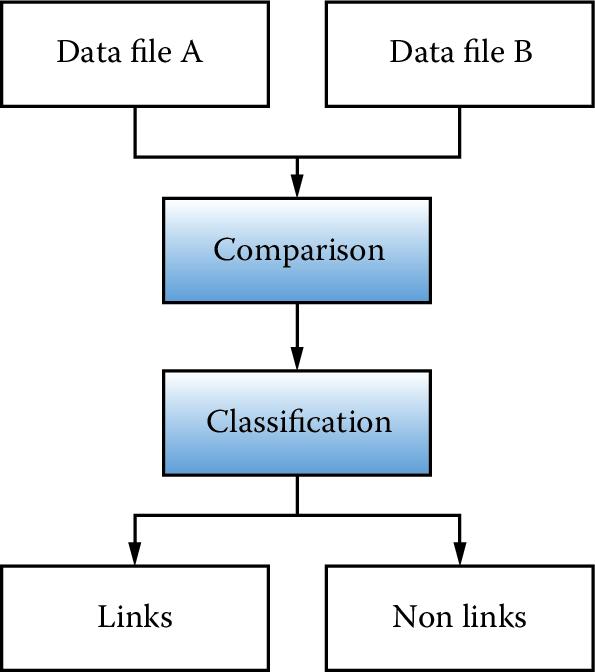
\includegraphics[width=0.7\linewidth]{ChapterLinkage/figures/fig3-1} 

}

\caption{The preprocessing pipeline}\label{fig:fig3-1}
\end{figure}

The canonical record linkage workflow process is shown in Figure
\ref{fig:fig3-1} for two data files, A and B. The goal is to identify
all pairs of records in the two data sets that correspond to the same
underlying individual. One approach is to compare all data units from
file A with all units in file B and classify all of the comparison
outcomes to decide whether or not the records match. In a perfect
statistical world the comparison would end with a clear determination of
links and nonlinks.

Alas, a perfect world does not exist, and there is likely to be noise in
the variables that are common to both data sets and that will be the
main identifiers for the record linkage. Although the original files A
and B are the starting point, the identifiers must be preprocessed
before they can be compared. Determining identifiers for the linkage and
deciding on the associated cleaning steps are extremely important, as
they result in a necessary reduction of the possible search space.

In the next section we begin our overview of the record linkage process
with a discussion of the main steps in data preprocessing. This is
followed by a section on approaches to record linkage that includes
rule-based, probabilistic, and machine learning algorithms. Next we
cover classification and evaluation of links, and we conclude with a
discussion of data privacy in record linkage.

\section{Preprocessing data for record
linkage}\label{preprocessing-data-for-record-linkage}

As noted in the introductory chapter, all data work involves
preprocessing, and data that need to be linked is no exception.
Preprocessing refers to a workflow that transforms messy and noisy data
into a well-defined, clearly structured, and quality-tested data set.
Elsewhere in this book, we discuss general strategies for data
preprocessing.\footnote{This topic (quality of data, preprocessing
  issues) is discussed in more detail in Chapter
  \protect\hyperlink{chap:intro}{Introduction}.} In this section, we
focus specifically on preprocessing steps relating to the choice of
input fields for the record linkage algorithm. Preprocessing for any
kind of a new data set is a complex and time-consuming process because
it is ``hands-on'': it requires judgment and cannot be effectively
automated. It may be tempting to minimize this demanding work under the
assumption that the record linkage algorithm will account for issues in
the data, but it is difficult to overstate the value of preprocessing
for record linkage quality. As Winkler notes: ``In situations of
reasonably high-quality data, preprocessing can yield a greater
improvement in matching efficiency than string comparators and
`optimized' parameters. In some situations, 90\% of the improvement in
matching efficiency may be due to preprocessing'' (Winkler
\protect\hyperlink{ref-winkler09}{2009}).

The first step in record linkage is to develop link keys, which are the
record fields that will be used to estimate if there is a link between
two records. These can include common identifiers like first and last
name. Survey and administrative data sets may include a number of
clearly identifying variables like address, birth date, and sex. Other
data sets, like transaction records or social media data, often will not
include address or birth date but may still include other identifying
fields like occupation, a list of interests, or connections on a social
network. Consider this chapter's illustrative example of the US Patent
and Trademark Office (USPTO) data (Ventura, Nugent, and Fuchs
\protect\hyperlink{ref-ventura2015seeing}{2015}):

\begin{quote}
USPTO maintains an online database of all patents issued in the United
States. In addition to identifying information about the patent, the
database contains each patent's list of inventors and assignees, the
companies, organizations, individuals, or government agencies to which
the patent is assigned. \ldots{} However, inventors and assignees in the
USPTO database are not given unique identification numbers, making it
difficult to track inventors and assignees across their patents or link
their information to other data sources.
\end{quote}

There are some basic precepts that are useful when considering
identifying fields. The more different values a field can take, the less
likely it is that two randomly chosen individuals in the population will
agree on those values. Therefore, fields that exhibit a wider range of
values are more powerful as link keys: names are much better link keys
than sex or year of birth.

\begin{center}\rule{0.5\linewidth}{\linethickness}\end{center}

\textbf{Example: Link keys in practice}

``A Harvard professor has re-identified the names of more than 40
percent of a sample of anonymous participants in a high-profile DNA
study, highlighting the dangers that ever greater amounts of personal
data available in the Internet era could unravel personal secrets.
\ldots{} Of the 1,130 volunteers Sweeney and her team reviewed, about
579 provided zip code, date of birth and gender, the three key pieces of
information she needs to identify anonymous people combined with
information from voter rolls or other public records. Of these, Sweeney
succeeded in naming 241, or 42 percent of the total. The Personal Genome
Project confirmed that 97 percent of the names matched those in its
database if nicknames and first name variations were included'' (Tanner
\protect\hyperlink{ref-forbesharvard}{2013}).

\begin{center}\rule{0.5\linewidth}{\linethickness}\end{center}

Complex link keys like addresses can be broken down into components so
that the components can be compared independently of one another. This
way, errors due to data quality can be further isolated. For example,
assigning a single comparison value to the complex fields ``1600
Pennsylvania'' and ``160 Pennsylvania Ave'' is less informative than
assigning separate comparison values to the street number and street
name portions of those fields. A record linkage algorithm that uses the
decomposed field can make more nuanced distinctions by assigning
different weights to errors in each component.

Sometimes a data set can include different variants of a field, like
legal first name and nickname. In these cases match rates can be
improved by including all variants of the field in the record
comparison. For example, if only the first list includes both variants,
and the second list has a single ``first name'' field that could be
either a legal first name or a nickname, then match rates can be
improved by comparing both variants and then keeping the better of the
two comparison outcomes. It is important to remember, however, that some
record linkage algorithms expect field comparisons to be somewhat
independent. In our example, using the outcome from both comparisons as
separate inputs into the probabilistic model we describe below may
result in a higher rate of false negatives. If a record has the same
value in the legal name and nickname fields, and if that value happens
to agree with the first name field in the second file, then the
agreement is being double-counted. By the same token, if a person in the
first list has a nickname that differs significantly from their legal
first name, then a comparison of that record to the corresponding record
will unfairly penalize the outcome because at least one of those name
comparisons will show a low level of agreement.

Preprocessing serves two purposes in record linkage. First, to correct
for issues in data quality that we described above. Second, to account
for the different ways that the input files were generated, which may
result in the same underlying data being recorded on different scales or
according to different conventions.

Once preprocessing is finished, it is possible to start linking the
records in the different data sets. In the next section we describe a
technique to improve the efficiency of the matching step.

\hypertarget{S:indexing}{\section{Indexing and
blocking}\label{S:indexing}}

There is a practical challenge to consider when comparing the records in
two files. If both files are roughly the same size, say \(100\) records
in the first and \(100\) records in the second file, then there are
\(10{,}000\) possible comparisons, because the number of pairs is the
product of the number of records in each file. More generally, if the
number of records in each file is approximately \(n\), then the total
number of possible record comparisons is approximately \(n^2\). Assuming
that there are no duplicate records in the input files, the proportion
of record comparisons that correspond to a link is only \(1/n\). If we
naively proceed with all \(n^2\) possible comparisons, the linkage
algorithm will spend the bulk of its time comparing records that are not
matches. Thus it is possible to speed up record linkage significantly by
skipping comparisons between record pairs that are not likely to be
linked.

Indexing refers to techniques that determine which of the possible
comparisons will be made in a record linkage application. The most used
technique for indexing is blocking. In this approach you construct a
``blocking key'' for each record by concatenating fields or parts of
fields. Two records with identical blocking keys are said to be in the
same block, and only records in the same block are compared. This
technique is effective because performing an exact comparison of two
blocking keys is a relatively quick operation compared to a full record
comparison, which may involve multiple applications of a fuzzy string
comparator.

\begin{center}\rule{0.5\linewidth}{\linethickness}\end{center}

\textbf{Example: Blocking in practice}

Given two lists of individuals, one might construct the blocking key by
concatenating the first letter of the last name and the postal code and
then ``blocking'' on first character of last name and postal code. This
reduces the total number of comparisons by only comparing those
individuals in the two files who live in the same locality and whose
last names begin with the same letter.

\begin{center}\rule{0.5\linewidth}{\linethickness}\end{center}

There are important considerations when choosing the blocking key.
First, the choice of blocking key creates a potential bias in the linked
data because true matches that do not share the same blocking key will
not be found. In the example, the blocking strategy could fail to match
records for individuals whose last name changed or who moved. Second,
because blocking keys are compared exactly, there is an implicit
assumption that the included fields will not have typos or other data
entry errors. In practice, however, the blocking fields will exhibit
typos. If those typos are not uniformly distributed over the population,
then there is again the possibility of bias in the linked data
set\footnote{This topic is discussed in more detail in Chapter
  \protect\hyperlink{chap:errors}{Data Quality and Inference Errors}.}.
One simple strategy for dealing with imperfect blocking keys is to
implement multiple rounds of blocking and matching. After the first set
of matches is produced, a new blocking strategy is deployed to search
for additional matches in the remaining record pairs.

Blocking based on exact field agreements is common in practice, but
there are other approaches to indexing that attempt to be more error
tolerant. For example, one may use clustering algorithms to identify
sets of similar records. In this approach an index key, which is
analogous to the blocking key above, is generated for both data sets and
then the keys are combined into a single list. A distance function must
be chosen and pairwise distances computed for all keys. The clustering
algorithm is then applied to the combined list, and only record pairs
that are assigned to the same cluster are compared. This is a
theoretically appealing approach but it has the drawback that the
similarity metric has to be computed for all pairs of records. Even so,
computing the similarity measure for a pair of blocking keys is likely
to be cheaper than computing the full record comparison, so there is
still a gain in efficiency. Whang et al.
(\protect\hyperlink{ref-whang2009entity}{2009}) provide a nice review of
indexing approaches.

In addition to reducing the computational burden of record linkage,
indexing plays an important secondary role. Once implemented, the
fraction of comparisons made that correspond to true links will be
significantly higher. For some record linkage approaches that use an
algorithm to find optimal parameters---like the probabilistic
approach---having a larger ratio of matches to nonmatches will produce a
better result.

\section{Matching}\label{matching}

The purpose of a record linkage algorithm is to examine pairs of records
and make a prediction as to whether they correspond to the same
underlying entity. (There are some sophisticated algorithms that examine
sets of more than two records at a time (Steorts, Hall, and Fienberg
\protect\hyperlink{ref-steorts2014smered}{2014}), but pairwise
comparison remains the standard approach.) At the core of every record
linkage algorithm is a function that compares two records and outputs a
``score'' that quantifies the similarity between those records.
Mathematically, the match score is a function of the output from
individual field comparisons: agreement in the first name field,
agreement in the last name field, etc. Field comparisons may be
binary---indicating agreement or disagreement---or they may output a
range of values indicating different levels of agreement. There are a
variety of methods in the statistical and computer science literature
that can be used to generate a match score, including nearest-neighbor
matching, regression-based matching, and propensity score matching. The
probabilistic approach to record linkage defines the match score in
terms of a likelihood ratio (Fellegi and Sunter
\protect\hyperlink{ref-FS69}{1969}).

\begin{center}\rule{0.5\linewidth}{\linethickness}\end{center}

\textbf{Example: Matching in practice}

Long strings, such as assignee and inventor names, are susceptible to
typographical errors and name variations. For example, none of Sony
Corporation, Sony Corporatoin and Sony Corp. will match using simple
exact matching. Similarly, David vs.~Dave would not match (Ventura,
Nugent, and Fuchs \protect\hyperlink{ref-ventura2015seeing}{2015}).

\begin{center}\rule{0.5\linewidth}{\linethickness}\end{center}

Comparing fields whose values are continuous is straightforward: often
one can simply take the absolute difference as the comparison value.
Comparing character fields in a rigorous way is more complicated. For
this purpose, different mathematical definitions of the distance between
two character fields have been defined. Edit distance, for example, is
defined as the minimum number of edit operations---chosen from a set of
allowed operations---needed to convert one string to another. When the
set of allowed edit operations is single-character insertions,
deletions, and substitutions, the corresponding edit distance is also
known as the Levenshtein distance. When transposition of adjacent
characters is allowed in addition to those operations, the corresponding
edit distance is called the Levenshtein--Damerau distance.

Edit distance is appealing because of its intuitive definition, but it
is not the most efficient string distance to compute. Another standard
string distance known as Jaro--Winkler distance was developed with
record linkage applications in mind and is faster to compute. This is an
important consideration because in a typical record linkage application
most of the algorithm run time will be spent performing field
comparisons. The definition of Jaro--Winkler distance is less intuitive
than edit distance, but it works as expected: words with more characters
in common will have a higher Jaro--Winkler value than those with fewer
characters in common. The output value is normalized to fall between 0
and 1. Because of its history in record linkage applications, there are
some standard variants of Jaro--Winkler distance that may be implemented
in record linkage software. Some variants boost the weight given to
agreement in the first few characters of the strings being compared.
Others decrease the score penalty for letter substitutions that arise
from common typos.

Once the field comparisons are computed, they must be combined to
produce a final prediction of match status. In the following sections we
describe three types of record linkage algorithms: rule-based,
probabilistic, and machine learning.

\subsection{Rule-based approaches}\label{rule-based-approaches}

A natural starting place is for a data expert to create a set of ad hoc
rules that determine which pairs of records should be linked. In the
classical record linkage setting where the two files have a number of
identifying fields in common, this is not the optimal approach. However,
if there are few fields in common but each file contains auxiliary
fields that may inform a linkage decision, then an ad hoc approach may
be appropriate.

\begin{center}\rule{0.5\linewidth}{\linethickness}\end{center}

\textbf{Example: Linking in practice}

Consider the problem of linking two lists of individuals where both
lists contain first name, last name, and year of birth. Here is one
possible linkage rule: link all pairs of records such that

\begin{itemize}
\item
  the Jaro--Winkler comparison of first names is greater than 0.9
\item
  the Jaro--Winkler comparison of last names is greater than 0.9
\item
  the first three digits of the year of birth are the same.
\end{itemize}

The result will depend on the rate of data errors in the year of birth
field and typos in the name fields.

\begin{center}\rule{0.5\linewidth}{\linethickness}\end{center}

By \emph{auxiliary field} we mean data fields that do not appear on both
data sets, but which may nonetheless provide information about whether
records should be linked. Consider a situation in which the first list
includes an occupation field and the second list includes educational
history. In that case one might create additional rules to eliminate
matches where the education was deemed to be an unlikely fit for the
occupation.

This method may be attractive if it produces a reasonable-looking set of
links from intuitive rules, but there are several pitfalls. As the
number of rules grows it becomes harder to understand the ways that the
different rules interact to produce the final set of links. There is no
notion of a threshold that can be increased or decreased depending on
the tolerance for false positive and false negative errors. The rules
themselves are not chosen to satisfy any kind of optimality, unlike the
probabilistic and machine learning methods. Instead, they reflect the
practitioner's domain knowledge about the data sets.

\subsection{Probabilistic record
linkage}\label{probabilistic-record-linkage}

In this section we describe the probabilistic approach to record
linkage, also known as the Fellegi--Sunter algorithm (Fellegi and Sunter
\protect\hyperlink{ref-FS69}{1969}). This approach dominates in
traditional record linkage applications and remains an effective and
efficient way to solve the record linkage problem today.

In this section we give a somewhat formal definition of the statistical
model underlying the algorithm. By understanding this model, one is
better equipped to define link keys and record comparisons in an optimal
way.

\begin{center}\rule{0.5\linewidth}{\linethickness}\end{center}

\textbf{Example: Usefulness of probabilistic record linkage}

In practice, it is typically the case that a researcher will want to
combine two or more data sets containing records for the same
individuals or units that possibly come from different sources. Unless
the sources all contain the same unique identifiers, linkage will likely
require matching on standardized text strings. Even standardized data
are likely to contain small differences that preclude exact matching as
in the matching example above. The Census Bureau's Longitudinal Business
Database (LBD) links establishment records from administrative and
survey sources. Exact numeric identifiers do most of the heavy lifting,
but mergers, acquisitions, and other actions can break these linkages.
Probabilistic record linkage on company names and/or addresses is used
to fix these broken linkages that bias statistics on business dynamics
(Jarmin and Miranda
\protect\hyperlink{ref-jarmin2002longitudinal}{2002}).

\begin{center}\rule{0.5\linewidth}{\linethickness}\end{center}

Let \(A\) and \(B\) be two lists of individuals whom we wish to link.
The product set \(A \times B\) contains all possible pairs of records
where the first element of the pair comes from \(A\) and the second
element of the pair comes from \(B\). A fraction of these pairs will be
matches, meaning that both records in the pair represent the same
underlying individual, but the vast majority of them will be nonmatches.
In other words, \(A \times B\) is the disjoint union of the set of
matches \(M\) and the set of nonmatches \(U\), a fact that we denote
formally by \(A \times B = M \cup U\).

Let \(\gamma\) be a vector-valued function on \(A \times B\) such that,
for \(a \in A\) and \(b \in B\), \(\gamma(a, b)\) represents the outcome
of a set of field comparisons between \(a\) and \(b\). For example, if
both \(A\) and \(B\) contain data on individuals' first names, last
names, and cities of residence, then \(\gamma\) could be a vector of
three binary values representing agreement in first name, last name, and
city. In that case \(\gamma(a, b) = (1, 1, 0)\) would mean that the
records \(a\) and \(b\) agree on first name and last name, but disagree
on city of residence.

For this model, the comparison outcomes in \(\gamma(a, b)\) are not
required to be binary, but they do have to be categorical: each
component of \(\gamma(a, b)\) should take only finitely many values.
This means that a continuous comparison outcome---such as output from
the string comparator---has to be converted to an ordinal value
representing levels of agreement. For example, one might create a
three-level comparison, using one level for exact agreement, one level
for approximate agreement defined as a Jaro--Winkler score greater than
0.85, and one level for nonagreement corresponding to a Jaro--Winkler
score less than 0.85.

If a variable being used in the comparison has a significant number of
missing values, it can help to create a comparison outcome level to
indicate missingness. Consider two data sets that both have middle
initial fields, and suppose that in one of the data sets the middle
initial is filled in only about half of the time. When comparing
records, the case where both middle initials are filled in but are not
the same should be treated differently from the case where one of the
middle initials is blank, because the first case provides more evidence
that the records do not correspond to the same person. We handle this in
the model by defining a three-level comparison for the middle initial,
with levels to indicate ``equal,'' ``not equal,'' and ``missing.''

Probabilistic record linkage works by weighing the probability of seeing
the result \(\gamma(a, b)\) if \((a, b)\) belongs to the set of matches
\(M\) against the probability of seeing the result if \((a, b)\) belongs
to the set of nonmatches \(U\). Conditional on \(M\) or \(U\), the
distribution of the individual comparisons defined by \(\gamma\) are
assumed to be mutually independent. The parameters that define the
marginal distributions of \(\gamma | M\) are called
\emph{\(m\)-weights}, and similarly the marginal distributions of
\(\gamma | U\) are called \emph{\(u\)-weights}.

In order to apply the Fellegi--Sunter method, it is necessary to choose
values for these parameters, \(m\)-weights and \(u\)-weights. With
labeled data---a pair of lists for which the match status is known---it
is straightforward to solve for optimal values. Training data are not
usually available, however, and the typical approach is to use
expectation maximization to find optimal values.

We have noted that primary motivation for record linkage is to create a
linked data set for analysis that will have a richer than either of the
input data sets alone. A natural application is to perform a linear
regression using a combination of variables from both files as
predictors. With all record linkage approaches it is a challenge to
understand how errors from the linkage process will manifest in the
regression. Probabilistic record linkage has an advantage over
rule-based and machine learning approaches in that there are theoretical
results concerning coefficient bias and errors (Scheuren and Winkler
\protect\hyperlink{ref-scheuren1993regression}{1993}; Lahiri and Larsen
\protect\hyperlink{ref-lahiri2005regression}{2005}). More recently,
Chipperfield and Chambers have developed an approach based on the
bootstrap to account for record linkage errors when making inferences
for cross-tabulated

\subsection{Machine learning approaches to record
linkage}\label{machine-learning-approaches-to-record-linkage}

Computer scientists have contributed extensively in parallel literature
focused on linking large data sets (Christen
\protect\hyperlink{ref-christen2012data}{2012}\protect\hyperlink{ref-christen2012data}{b}).
Their focus is on identifying potential links using approaches that are
fast, adaptive, and scalable, and approaches are developed based on work
in network analysis and machine learning.

While simple blocking as described in Section
\protect\hyperlink{S:indexing}{Indexing and Blocking} is standard in
Fellegi--Sunter applications, machine learning based approaches are
likely to use the more sophisticated clustering approach to indexing.
Indexing may also use network information to include, for example,
records for individuals that have a similar place in a social graph.
When linking lists of researchers, one might specify that comparisons
should be made between records that share the same address, have patents
in the same patent class, or have overlapping sets of coinventors. These
approaches are known as semantic blocking, and the computational
requirements are similar to standard blocking (Christen
\protect\hyperlink{ref-christen2012data}{2012}\protect\hyperlink{ref-christen2012data}{b}).

In recent years machine learning approaches\footnote{This topic is
  discussed in more detail in Chapter
  \protect\hyperlink{chap:ml}{Machine Learning}.} have been applied to
record Linkage. As Wick et al.
(\protect\hyperlink{ref-wick2013joint}{2013}) note:

\begin{quote}
Entity resolution, the task of automatically determining which mentions
refer to the same real-world entity, is a crucial aspect of knowledge
base construction and management. However, performing entity resolution
at large scales is challenging because (1) the inference algorithms must
cope with unavoidable system scalability issues and (2) the search space
grows exponentially in the number of mentions. Current conventional
wisdom declares that performing coreference at these scales requires
decomposing the problem by first solving the simpler task of
entity-linking (matching a set of mentions to a known set of KB
entities), and then performing entity discovery as a post-processing
step (to identify new entities not present in the KB). However, we argue
that this traditional approach is harmful to both entity-linking and
overall coreference accuracy. Therefore, we embrace the challenge of
jointly modeling entity-linking and entity discovery as a single entity
resolution problem.
\end{quote}

Figure \ref{fig:fig3-2} provides a useful comparison between classical
record linkage and learning-based approaches. In machine learning there
is a statistical model and an algorithm for ``learning'' the optimal set
of parameters to use. The learning algorithm relies on a training data
set. In record linkage, this would be a curated data set with true and
false matches labeled as such. See (Ventura, Nugent, and Fuchs
\protect\hyperlink{ref-ventura2015seeing}{2015}) for an example and a
discussion of how a training data set was created for the problem of
disambiguating inventors in the USPTO database. Once optimal parameters
are computed from the training data, the predictive model can be applied
to unlabeled data to find new links. The quality of the training data
set is critical; the model is only as good as the data it is trained on.

\begin{figure}

{\centering 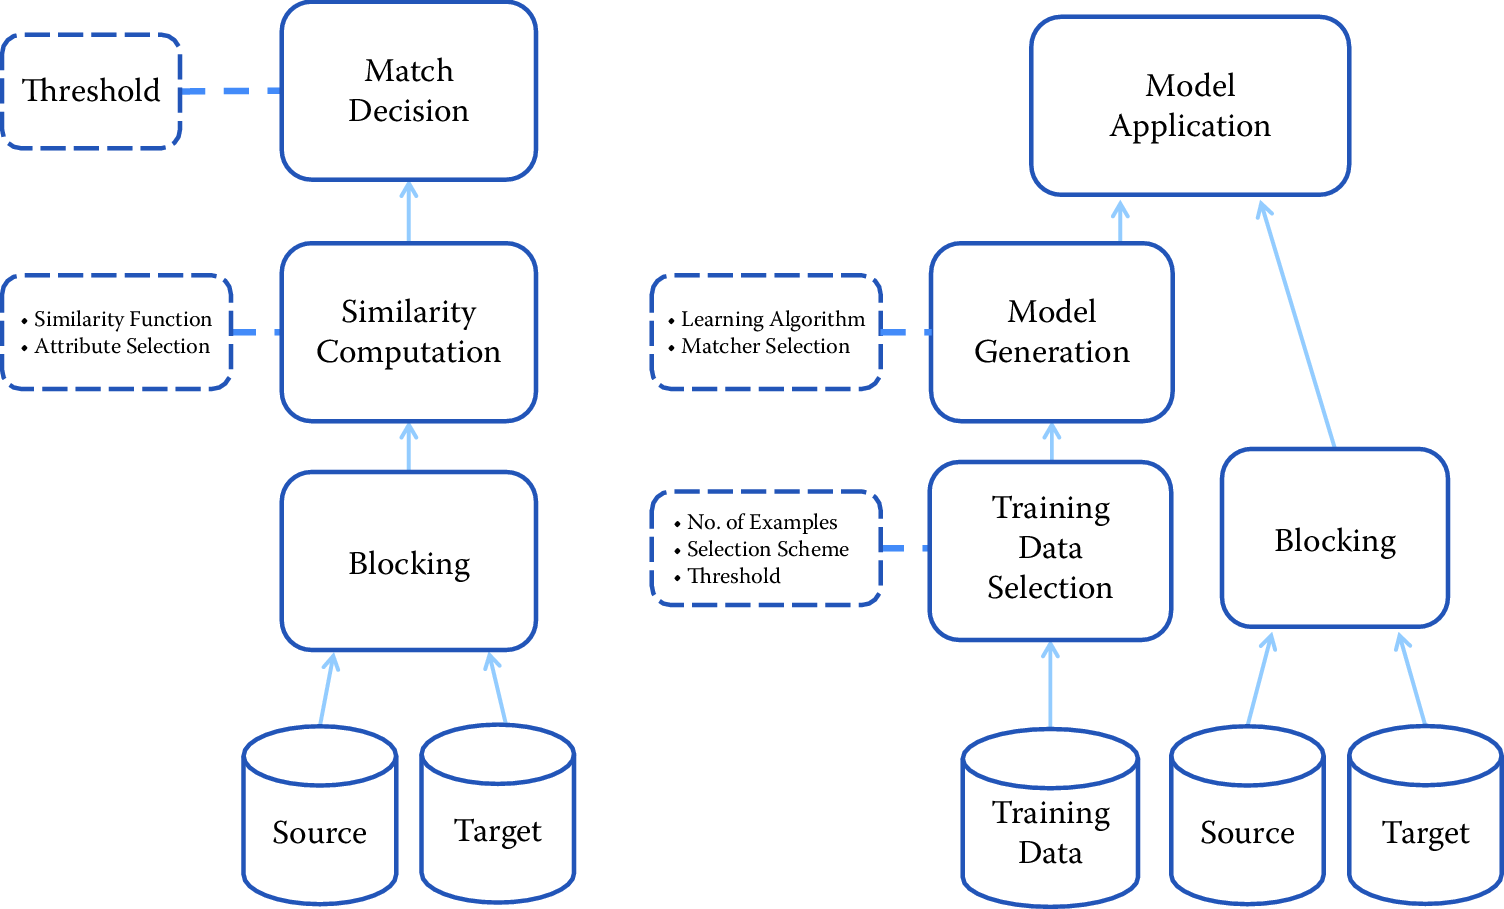
\includegraphics[width=0.7\linewidth]{ChapterLinkage/figures/fig3-2} 

}

\caption{Probabilistic (left) vs. machine learning (right) approaches to linking. Source: @kopcke2010evaluation}\label{fig:fig3-2}
\end{figure}

As shown in Figure \ref{fig:fig3-2}, a major difference between
probabilistic and machine learning approaches is the need for labeled
training data to implement the latter approach. Usually training data
are created through a painstaking process of clerical review. After an
initial round of record linkage, a sample of record pairs that are not
clearly matches or nonmatches is given to a research assistant who makes
the final determination. In some cases it is possible to create training
data by automated means. For example, when there is a subset of the
complete data that contains strongly identifying fields. Suppose that
both of the candidate lists contain name and date of birth fields and
that in the first list the date of birth data are complete, but in the
second list only about 10\% of records contain date of birth. For
reasonably sized lists, name and date of birth together will be a nearly
unique identifier. It is then possible to perform probabilistic record
linkage on the subset of records with date of birth and be confident
that the error rates would be small. If the subset of records with date
of birth is representative of the complete data set, then the output
from the probabilistic record linkage can be used as ``truth'' data.

Given a quality training data set, machine learning approaches may have
advantages over probabilistic record linkage. There are many published
studies on the effectiveness of random forests and other machine
learning algorithms for record linkage. Christen and Ahmed et al.
provide some pointers (Christen
\protect\hyperlink{ref-christen2012survey}{2012}\protect\hyperlink{ref-christen2012survey}{a};
Elmagarmid, Ipeirotis, and Verykios
\protect\hyperlink{ref-elmagarmid2007duplicate}{2007}).

\subsection{Disambiguating networks}\label{disambiguating-networks}

The problem of disambiguating entities in a network is closely related
to record linkage: in both cases the goal is to consolidate multiple
records corresponding to the same entity. Rather than finding the same
entity in two data sets, however, the goal in network disambiguation is
to consolidate duplicate records in a network data set. By network we
mean that the data set contains not only typical record fields like
names and addresses but also information about how entities relate to
one another: entities may be coauthors, coinventors, or simply friends
in a social network.

The record linkage techniques that we have described in this chapter can
be applied to disambiguate a network. To do so, one must convert the
network to a form that can be used as input into a record linkage
algorithm. For example, when disambiguating a social network one might
define a field comparison whose output gives the fraction of friends in
common between two records. Ventura et al. demonstrated the relative
effectiveness of the probabilistic method and machine learning
approaches to disambiguating a database of inventors in the USPTO
database (Ventura, Nugent, and Fuchs
\protect\hyperlink{ref-ventura2015seeing}{2015}). Another approach is to
apply clustering algorithms from the computer science literature to
identify groups of records that are likely to refer to the same entity.
Huang et al. (\protect\hyperlink{ref-HEG06}{2006}) have developed a
successful method based on an efficient computation of distance between
individuals in the network. These distances are then fed into the DBSCAN
clustering algorithm to identify unique entities.

\section{Classification}\label{classification}

Once the match score for a pair of records has been computed using the
probabilistic or random forest method, a decision has to be made whether
the pair should be linked. This requires classifying the pair as either
a ``true'' or a ``false'' match. In most cases, a third classification
is required---sending for manual review and classification.

\subsection{Thresholds}\label{S:thresholds}

In the probabilistic and random forest approaches, both of which output
a ``match score'' value, a classification is made by establishing a
threshold \(T\) such that all records with a match score greater than
\(T\) are declared to be links. Because of the way these algorithms are
defined, the match scores are not meaningful by themselves and the
threshold used for one linkage application may not be appropriate for
another application. Instead, the classification threshold must be
established by reviewing the model output.

Typically one creates an output file that includes pairs of records that
were compared along with the match score. The file is sorted by match
score and the reviewer begins to scan the file from the highest match
scores to the lowest. For the highest match scores the record pairs will
agree on all fields and there is usually no question about the records
being linked. However, as the scores decrease the reviewer will see more
record pairs whose match status is unclear (or that are clearly
nonmatches) mixed in with the clear matches. There are a number of ways
to proceed, depending on the resources available and the goal of the
project.

Rather than set a single threshold, the reviewer may set two thresholds
\(T_1 > T_2\). Record pairs with a match score greater than \(T_1\) are
marked as matches and removed from further consideration. The set of
record pairs with a match score between \(T_1\) and \(T_2\) are believed
to contain significant numbers of matches and nonmatches. These are sent
to clerical review, meaning that research assistants will make a final
determination of match status. The final set of links will include clear
matches with a score greater than \(T_1\) as well as the record pairs
that pass clerical review. If the resources are available for this
approach and the initial threshold \(T_1\) is set sufficiently high,
then the resulting data set will contain a minimal number of false
positive links. The collection of record pairs with match scores between
\(T_1\) and \(T_2\) is sometimes referred to as the clerical review
region.

The clerical review region generally contains many more pairs than the
set of clear matches, and it can be expensive and time-consuming to
review each pair. Therefore, a second approach is to establish tentative
threshold \(T\) and send only a sample of record pairs with scores in a
neighborhood of \(T\) to clerical review. This results in data on the
relative numbers of true matches and true nonmatches at different score
levels, as well as the characteristics of record pairs that appear at a
given level. Based on the review and the relative tolerance for false
positive errors and false negative errors, a final threshold \(T'\) is
set such that pairs with a score greater than \(T'\) are considered to
be matches.

After viewing the results of the clerical review, it may be determined
that the parameters to the record linkage algorithm could be improved to
create a clearer delineation between matches and nonmatches. For
example, a research assistant may determine that many potential false
positives appear near the tentative threshold because the current set of
record linkage parameters is giving too much weight to agreement in
first name. In this case the reviewer may decide to update the record
linkage model to produce an improved set of match scores. The update may
consist in an ad hoc adjustment of parameters, or the result of the
clerical review may be used as training data and the parameter-fitting
algorithm may be run again. An iterative approach like this is common
when first linking two data sets because the clerical review process can
improve one's understanding of the data sets involved.

Setting the threshold value higher will reduce the number of false
positives (record pairs for which a link is incorrectly predicted) while
increasing the number of false negatives (record pairs that should be
linked but for which a link is not predicted). The proper tradeoff
between false positive and false negative error rates will depend on the
particular application and the associated loss function, but there are
some general concerns to keep in mind. Both types of errors create bias,
which can impact the generalizability of analyses conducted on the
linked data set. Consider a simple regression on the linked data that
includes fields from both data sets. If the threshold is too high, then
the linked data will be biased toward records with no data entry errors
or missing values, and whose fields did not change over time. This set
of records may not be representative of the population as a whole. If a
low threshold is used, then the set of linked records will contain more
pairs that are not true links and the variables measured in those
records are independent of each other. Including these records in a
regression amounts to adding statistical noise to the data.

\subsection{One-to-one links}\label{one-to-one-links}

In the probabilistic and machine learning approaches to record linkage
that we have described, each record pair is compared and a link is
predicted independently of all other record pairs. Because of the
independence of comparisons, one record in the first file may be
predicted to link to multiple records in the second file. Under the
assumption that each input file has been deduplicated, at most one of
these predictions can correspond to a true link. For many applications
it is preferable to extract a set of ``best'' links with the property
that each record in one file links to at most one record in the second
file. A set of links with this property is said to be one-to-one.

One possible definition of ``best'' is a set of one-to-one links such
that the sum of the match scores of all included links is maximal. This
is an example of what is known as the \emph{assignment problem} in
combinatorial optimization. In the linear case above, where we care
about the sum of match scores, the problem can be solved exactly using
the Hungarian algorithm (Kuhn
\protect\hyperlink{ref-kuhn2005hungarian}{2005}).

\section{Record linkage and data
protection}\label{record-linkage-and-data-protection}

In many social science applications data sets there is no need for data
to include identifying fields like names and addresses. These fields may
be left out intentionally out of concern for privacy\footnote{See
  Chapter \protect\hyperlink{chap:privacy}{Privacy and Confidentiality}.},
or they may simply be irrelevant to the research question. For record
linkage, however, names and addresses are among the best possible
identifiers. We describe two approaches to the problem of balancing
needs for both effective record linkage and privacy.

The first approach is to establish a trusted third party or safe center.
The concept of trusted third parties (TTPs) is well known in
cryptography. In the case of record linkage, a third party takes a place
between the data owners and the data users, and it is this third party
that actually performs the linkage work. Both the data owners and data
users trust the third party in the sense that it assumes responsibility
for data protection (data owners) and data competence (data users) at
the same time. No party other than the TTP learns about the private data
of the other parties. After record linkage only the linked records are
revealed, with no identifiers attached. The TTP ensures that the
released linked data set cannot be relinked to any of the source data
sets. Possible third parties are safe centers, which are operated by
lawyers, or official trusted institutions like the US Census Bureau.

The second approach is known as privacy-preserving record linkage. The
goal of this approach is to find the same individual in separate data
files without revealing the identity of the individual (Clifton et al.
\protect\hyperlink{ref-Clifton06}{2006}). In privacy-preserving record
linkage, cryptographic procedures are used to encrypt or hash
identifiers before they are shared for record linkage. Many of these
procedures require exact matching of the identifiers, however, and do
not tolerate any errors in the original identifiers. This leads to
information loss because it is not possible to account for typos or
other small variations in hashed fields. To account for this, Schnell
has developed a method to calculate string similarity of encrypted
fields using bloom filters (Schnell
\protect\hyperlink{ref-schnell2014efficient}{2014}; Schnell, Bachteler,
and Reiher \protect\hyperlink{ref-schnell2009privacy}{2009}).

In many countries these approaches are combined. For example, when the
UK established the ADRN, the latter established the concept of trusted
third parties. That third party is provided with data in which
identifying fields have been hashed. This solves the challenge of trust
between the different parties. Some authors argue that transparency of
data use and informed consent will help to build trust. In the context
of big data this is more challenging\footnote{This topic is discussed in
  more detail in Chapter \protect\hyperlink{chap:privacy}{Privacy and
  Confidentiality}.}.

\section{Summary}\label{summary-1}

Accurate record linkage is critical to creating high-quality data sets
for analysis. However, outside of a few small centers for record linkage
research, linking data sets historically relied on artisan approaches,
particularly for parsing and cleaning data sets. As the creation and use
of big data increases, so does the need for systematic record linkage.
The history of record linkage is long by computer science standards, but
new data challenges encourage the development of new approaches like
machine learning methods, clustering algorithms, and privacy-preserving
record linkage.

Record linkage stands on the boundary between statistics, information
technology, and privacy. We are confident that there will continue to be
exciting developments in this field in the years to come.

\section{Resources}\label{resources}

Out of many excellent resources on the subject, we note the following:

\begin{itemize}
\item
  We strongly recommend Christen's book (Christen
  \protect\hyperlink{ref-christen2012data}{2012}\protect\hyperlink{ref-christen2012data}{b}).
\item
  There is a wealth of information available on the ADRN website
  (Economic and Social Research Council
  \protect\hyperlink{ref-EconomicandSocialResearchCouncil2016}{2016}).
\item
  Winkler has a series of high-quality survey articles (Winkler
  \protect\hyperlink{ref-WICS:WICS1317}{2014}).
\item
  The German Record Linkage Center is a resource for research, software,
  and ongoing conference activities (Schnell
  \protect\hyperlink{ref-Schnell2016}{2016}).
\item
  The \emph{Record Linkage} workbook of Chapter
  \protect\hyperlink{chap:workbooks}{Workbooks} provides an introduction
  to probabilistic record linkage with Python.\footnote{See
    \url{https://workbooks.coleridgeinitiative.org}.}
\end{itemize}

\hypertarget{chap:db}{\chapter{Databases}\label{chap:db}}

\textbf{Ian Foster and Pascal Heus}

Once data have been collected and linked, it is necessary to store and
organize them. Many social scientists are used to working with one
analytical file, often in SAS, Stata, SPSS, or R. But most organizations
store (or should store) their data in databases, which makes it critical
for social scientists to learn how to create, manage, and use databases
for data storage and analysis. This chapter describes the concept of
databases and introduces different types of databases and analysis
languages (in particular, relational databases and SQL, respectively)
that allow storing and organizing of data for rapid and efficient data
exploration and analysis.

\section{Introduction}\label{sec:db:intro}

We turn now to the question of how to store, organize, and manage the
data used in data-intensive social science. As the data with which you
work grow in volume and diversity, effective data management becomes
increasingly important to avoid scale and complexity from overwhelming
your research processes. In particular, when you deal with data that are
frequently updated, with changes made by different people, you will want
to use database management systems (DBMSs) instead of maintaining data
in text files or within siloed statistical packages such as SAS, SPSS,
Stata, and R. Indeed, we go so far as to say: if you take away
\emph{just one thing} from this book (or at least from this chapter), it
should be this: \emph{Use a database!}

As we explain in this chapter, DBMSs greatly simplify data management.
They require a little bit of effort to set up, but are worth it. They
permit large amounts of data to be organized in multiple ways that allow
for efficient and rapid exploration via query languages; durable and
reliable storage that maintain data consistency; scaling to large data
sizes; and intuitive analysis, both within the DBMS itself and via
connectors to other data analysis packages and tools. DBMSs have become
a critical component of most real-world systems, from handling
transactions in financial systems to delivering data to power websites,
dashboards, and software that we use every day. If you are using a
production-level enterprise system, chances are there is a database in
the back-end. They are multi-purpose and well suited for organizing
social science data and for supporting data exploration and analysis.

DBMSs make many easy things trivial, and many hard things easy. They are
easy to use but can appear daunting at first. A basic understanding of
databases and of when and how to use DBMSs is an important element of
the social data scientist's knowledge base. We therefore provide in this
chapter an introduction to databases and how to use them. We describe
different types of databases and their various features, and how they
can be used in different contexts. We describe basic features like how
to get started, setting up a database schema, ingesting data, querying
and analyzing data within a database, and getting results out. We also
discuss how to link from databases to other tools, such as Python, R,
and (if you have to) Stata.

\hypertarget{sec:db:when}{\section{DBMS: When and
why}\label{sec:db:when}}

Consider the following three data sets:

\begin{enumerate}
\def\labelenumi{\arabic{enumi}.}
\item
  10,000 records describing research grants, each specifying the
  principal investigator, institution, research area, proposal title,
  award date, and funding amount in a comma-separated-value (CSV)
  format.
\item
  10 million records in a variety of formats from funding agencies, web
  APIs, and institutional sources describing people, grants, funding
  agencies, and patents.
\item
  10 billion Twitter messages and associated metadata---around 10
  terabytes (\(10^{13}\) bytes) in total, and increasing at a terabyte a
  month.
\end{enumerate}

Which tools should you use to manage and analyze these data sets? The
answer depends on the specifics of the data, the analyses that you want
to perform, and the life cycle within which data and analyses are
embedded. Table \ref{tab:table4-1} summarizes relevant factors, which we
now discuss.

\begin{longtable}[]{@{}l@{}}
\caption{\label{tab:table4-1} When to use different data management and
analysis technologies}\tabularnewline
\toprule
\begin{minipage}[b]{0.89\columnwidth}\raggedright\strut
\textbf{When to use different data management and analysis
technologies}\strut
\end{minipage}\tabularnewline
\midrule
\endfirsthead
\toprule
\begin{minipage}[b]{0.89\columnwidth}\raggedright\strut
\textbf{When to use different data management and analysis
technologies}\strut
\end{minipage}\tabularnewline
\midrule
\endhead
\begin{minipage}[t]{0.89\columnwidth}\raggedright\strut
\textbf{Text files, spreadsheets, and scripting language}\strut
\end{minipage}\tabularnewline
\begin{minipage}[t]{0.89\columnwidth}\raggedright\strut
• Your data are small\strut
\end{minipage}\tabularnewline
\begin{minipage}[t]{0.89\columnwidth}\raggedright\strut
• Your analysis is simple\strut
\end{minipage}\tabularnewline
\begin{minipage}[t]{0.89\columnwidth}\raggedright\strut
• You do not expect to repeat analyses over time\strut
\end{minipage}\tabularnewline
\begin{minipage}[t]{0.89\columnwidth}\raggedright\strut
\textbf{Statistical packages}\strut
\end{minipage}\tabularnewline
\begin{minipage}[t]{0.89\columnwidth}\raggedright\strut
• Your data are modest in size\strut
\end{minipage}\tabularnewline
\begin{minipage}[t]{0.89\columnwidth}\raggedright\strut
• Your analysis maps well to your chosen statistical package\strut
\end{minipage}\tabularnewline
\begin{minipage}[t]{0.89\columnwidth}\raggedright\strut
\textbf{Relational database}\strut
\end{minipage}\tabularnewline
\begin{minipage}[t]{0.89\columnwidth}\raggedright\strut
• Your data are structured\strut
\end{minipage}\tabularnewline
\begin{minipage}[t]{0.89\columnwidth}\raggedright\strut
• Your data are large\strut
\end{minipage}\tabularnewline
\begin{minipage}[t]{0.89\columnwidth}\raggedright\strut
• You will be analyzing changed versions of your data over time\strut
\end{minipage}\tabularnewline
\begin{minipage}[t]{0.89\columnwidth}\raggedright\strut
• You want to share your data and analyses with others\strut
\end{minipage}\tabularnewline
\begin{minipage}[t]{0.89\columnwidth}\raggedright\strut
\textbf{NoSQL database}\strut
\end{minipage}\tabularnewline
\begin{minipage}[t]{0.89\columnwidth}\raggedright\strut
• Your data are unstructured\strut
\end{minipage}\tabularnewline
\begin{minipage}[t]{0.89\columnwidth}\raggedright\strut
• Your data are extremely large\strut
\end{minipage}\tabularnewline
\begin{minipage}[t]{0.89\columnwidth}\raggedright\strut
* Your analysis will happen mostly outside the database in a programming
language\strut
\end{minipage}\tabularnewline
\begin{minipage}[t]{0.89\columnwidth}\raggedright\strut
\strut
\end{minipage}\tabularnewline
\bottomrule
\end{longtable}

In the case of data set 1 (10,000 records describing research grants),
it may be feasible to leave the data in their original file, use
spreadsheets, pivot tables, or write programs in \textbf{scripting
languages}\footnote{A scripting language is a programming language used
  to automate tasks that could otherwise be performed one by one by the
  user.} such as Python or R to analyze the data in those files. For
example, someone familiar with such languages can quickly create a
script to extract from data set 1 all grants awarded to one
investigator, compute average grant size, and count grants made each
year in different areas.

However, this approach also has disadvantages. Scripts do not provide
inherent control over the file structure. This means that if you obtain
new data in a different format, your scripts need to be updated. You
cannot just run them over the newly acquired file. Scripts can also
easily become unreasonably slow as data volumes grow. A Python or R
script will not take long to search a list of 1,000 grants to find those
that pertain to a particular institution. But what if you have
information about 1 million grants, and for each grant you want to
search a list of 100,000 investigators, and for each investigator, you
want to search a list of 10 million papers to see whether that
investigator is listed as an author of each paper? You now have
\(1{,}000{,}000 \times 100{,}000 \times 10{,}000{,}000 = 10^{18}\)
comparisons to perform. Your simple script may now run for hours or even
days. You can speed up the search process by constructing indices, so
that, for example, when given a grant, you can find the associated
investigators in constant time rather than in time proportional to the
number of investigators. However, the construction of such indices is
itself a time-consuming and error-prone process.

For these reasons, the use of scripting languages alone for data
analysis is rarely to be recommended. This is not to say that all
analysis computations can be performed in database systems. A
programming language will also often be needed. But many data access and
manipulation computations are best handled in a database.

Researchers in the social sciences frequently use statistical packages
such as R, SAS, SPSS, and Stata for data analysis. Because these systems
integrate some data management, statistical analysis, and graphics
capabilities in a single package, a researcher can often carry out a
data analysis project of modest size within the same environment.
However, each of these systems has limitations that hinder its use for
modern social science research, especially as data grow in size and
complexity.

Take Stata, for example. Stata loads the entire data set into the
computer's working memory, and thus you would have no problems loading
data set 1. However, depending on your computer's memory, it could have
problems dealing with with data set 2 and most likely would not be able
to handle data set 3. In addition, you would need to perform this data
loading step each time you start working on the project, and your
analyses would be limited to what Stata can do. SAS can deal with larger
data sets, but is renowned for being hard to learn and use. Of course
there are workarounds in statistical packages. For example, in Stata you
can deal with larger file sizes by choosing to only load the variables
or cases that you need for the analysis (Kohler and Kreuter
\protect\hyperlink{ref-kohler2012datenanalyse}{2012}). Likewise, you can
deal with more complex data by creating a system of files that each can
be linked as needed for a particular analysis through a common
identifier variable.\footnote{For example, the Panel Study of Income
  Dynamics (\url{http://psidonline.isr.umich.edu}) has a series of files
  that are related and can be combined through common identifier
  variables (Institute for Social Research
  \protect\hyperlink{ref-PSIDguide}{2013}).}

The ad hoc approaches to problems of scale mentioned in the preceding
paragraph are provided as core functions in most DBMSs, and thus rather
than implement such inevitably limited workarounds, you will usually be
well advised to set up a database. A database is especially valuable if
you find yourself in a situation where the data set is constantly
updated by different users, if groups of users have different rights to
use your data or should only have access to subsets of the data, or if
the analysis takes place on a server that sends results to a client
(browser). Some statistics packages also have difficulty working with
more than one data source at a time---something that DBMSs are designed
to do well.

Alas, databases are not perfectly suited for every need. For example, in
social science research, the reproducibility of our analysis is critical
and hence versioning of the data used for analysis is critical. Most
databases do not do provide versioning out of the box. Typically, they
do keep a log of all operations performed (inserting, updating, updating
data for example), which can facilitate versioning and rollbacks, but we
often need to configure the database to allow versioning and support
reproducibility.

These considerations bring us to the topic of this chapter, namely
\textbf{database management systems}. A DBMS\footnote{DBMS is a system
  that interacts with users, other applications, and the database itself
  to capture and analyze data.} handles all of the issues listed above,
and more. As we will see below when we look at concrete examples, a DBMS
allows us to define a logical design that fits the structure of our
data. The DBMS then creates a \emph{data model} (more on this below)
that allows these data to be stored, queried, and updated efficiently
and reliably on disk, thus providing independence from underlying
physical storage. It supports efficient access to data through
\emph{query languages} and (somewhat) automatic optimization of those
queries to permit fast analysis. Importantly, it also support concurrent
access by multiple users, which is not an option for file-based data
storage. It supports \emph{transactions}, meaning that any update to a
database is performed in its entirety or not at all, even in the face of
computer failures or multiple concurrent updates. It also reduces the
time spent both by analysts, by making it easy to express complex
analytical queries concisely, and on data administration, by providing
simple and uniform data administration interfaces.

A \emph{database} is a structured collection of data about entities and
their relationships. It models real-world objects---both entities (e.g.,
grants, investigators, universities) and relationships (e.g., ``Steven
Weinberg'' works at ``University of Texas at Austin'')---and captures
structure in ways that allow these entities and relationships to be
queried for analysis. A \emph{database management system} is a software
suite designed to safely store and efficiently manage databases, and to
assist with the maintenance and discovery of the relationships that
database represents. In general, a DBMS encompasses three key
components: its \emph{data model} (which defines how data are
represented: see Box \protect\hyperlink{box:db1}{Data model}, its
\emph{query language} (which defines how the user interacts with the
data), and support for \emph{transactions and crash recovery} (to ensure
reliable execution despite system failures).\footnote{Some key DBMS
  features are often lacking in standard statistical packages: a
  standard query language (with commands that allow analyses or data
  manipulation on a subgroup of cases defined during the analysis, for
  example ``group by \ldots{},'' ``order by \ldots{}''), keys (for speed
  improvement), and an explicit model of a relational data structure.}

\begin{center}\rule{0.5\linewidth}{\linethickness}\end{center}

\textbf{Box: Data model}

A \emph{data model} specifies the data elements associated with the
domain we are analyzing, the properties of those data elements, and how
those data elements relate to one another. In developing a data model,
we commonly first identity the entities that are to be modeled and then
define their properties and relationships. For example, when working on
the science of science policy (see Figure \ref{fig:fig2}, the entities
include people, products, institutions, and funding, each of which has
various properties (e.g., for a person, their name, address, employer);
relationships include ``is employed by'' and ``is funded by.'' This
conceptual data model can then be translated into relational tables or
some other database representation, as we describe next.

\begin{center}\rule{0.5\linewidth}{\linethickness}\end{center}

Hundreds of different open source, commercial, and cloud-hosted versions
DBMSs are available and new ones pop up every day. However, you only
need to understand a relatively small number of concepts and major
database types to make sense of this diversity. Table \ref{tab:table4-3}
defines the major classes of DBMSs that we will consider in this
chapter. We consider only a few of these in any detail.

Relational DBMSs are the most widely used systems, and will be the
optimal solution for many social science data analysis purposes. We
describe relational DBMSs in detail below, but in brief, they allow for
the efficient storage, organization, and analysis of large quantities of
\emph{tabular} data\footnote{Sometimes, as discussed in Chapter
  \protect\hyperlink{chap:link}{Record Linkage}, the links are one to
  one and sometimes one to many.}: data organized as tables, in which
rows represent entities (e.g., research grants) and columns represent
attributes of those entities (e.g., principal investigator, institution,
funding level). The associated Structured Query Language (SQL) can then
be used to perform a wide range of tasks, which are executed with high
efficiency due to sophisticated indexing and query planning techniques.

While relational DBMSs have dominated the database world for decades,
other database technologies have become popular for various classes of
applications in recent years. As we will see, the design of these
alternative \emph{NoSQL DBMSs} is typically motivated by a desire to
scale the quantities of data and/or number of users that can be
supported and/or to deal with unstructured data that are not easily
represented in tabular form. For example, a key--value store can
organize large numbers of records, each of which associates an arbitrary
key with an arbitrary value. These stores, and in particular variants
called \emph{document stores} that permit text search on the stored
values, are widely used to organize and process the billions of records
that can be obtained from web crawlers. We review below some of these
alternatives and the factors that may motivate their use.

\begin{longtable}[]{@{}lllll@{}}
\caption{\label{tab:table4-3} Types of databases: relational (first row) and
various types of NoSQL (other rows)}\tabularnewline
\toprule
\begin{minipage}[b]{0.07\columnwidth}\raggedright\strut
\textbf{Type}\strut
\end{minipage} & \begin{minipage}[b]{0.16\columnwidth}\raggedright\strut
\textbf{Examples}\strut
\end{minipage} & \begin{minipage}[b]{0.22\columnwidth}\raggedright\strut
\textbf{Advantages}\strut
\end{minipage} & \begin{minipage}[b]{0.20\columnwidth}\raggedright\strut
\textbf{Disadvantages}\strut
\end{minipage} & \begin{minipage}[b]{0.21\columnwidth}\raggedright\strut
\textbf{Uses}\strut
\end{minipage}\tabularnewline
\midrule
\endfirsthead
\toprule
\begin{minipage}[b]{0.07\columnwidth}\raggedright\strut
\textbf{Type}\strut
\end{minipage} & \begin{minipage}[b]{0.16\columnwidth}\raggedright\strut
\textbf{Examples}\strut
\end{minipage} & \begin{minipage}[b]{0.22\columnwidth}\raggedright\strut
\textbf{Advantages}\strut
\end{minipage} & \begin{minipage}[b]{0.20\columnwidth}\raggedright\strut
\textbf{Disadvantages}\strut
\end{minipage} & \begin{minipage}[b]{0.21\columnwidth}\raggedright\strut
\textbf{Uses}\strut
\end{minipage}\tabularnewline
\midrule
\endhead
\begin{minipage}[t]{0.07\columnwidth}\raggedright\strut
Relational database\strut
\end{minipage} & \begin{minipage}[t]{0.16\columnwidth}\raggedright\strut
MySQL, PostgreSQL, Oracle, SQL Server, Teradata\strut
\end{minipage} & \begin{minipage}[t]{0.22\columnwidth}\raggedright\strut
Consistency (ACID)\strut
\end{minipage} & \begin{minipage}[t]{0.20\columnwidth}\raggedright\strut
Fixed schema; typically harder to scale\strut
\end{minipage} & \begin{minipage}[t]{0.21\columnwidth}\raggedright\strut
Transactional systems: order processing, retail, hospitals, etc.\strut
\end{minipage}\tabularnewline
\begin{minipage}[t]{0.07\columnwidth}\raggedright\strut
Key--value store\strut
\end{minipage} & \begin{minipage}[t]{0.16\columnwidth}\raggedright\strut
Dynamo, Redis\strut
\end{minipage} & \begin{minipage}[t]{0.22\columnwidth}\raggedright\strut
Dynamic schema; easy scaling; high throughput\strut
\end{minipage} & \begin{minipage}[t]{0.20\columnwidth}\raggedright\strut
Not immediately consistent; no higher-level queries\strut
\end{minipage} & \begin{minipage}[t]{0.21\columnwidth}\raggedright\strut
Web applications\strut
\end{minipage}\tabularnewline
\begin{minipage}[t]{0.07\columnwidth}\raggedright\strut
Column store\strut
\end{minipage} & \begin{minipage}[t]{0.16\columnwidth}\raggedright\strut
Cassandra, HBase\strut
\end{minipage} & \begin{minipage}[t]{0.22\columnwidth}\raggedright\strut
Same as key--value; distributed; better compression at column
level\strut
\end{minipage} & \begin{minipage}[t]{0.20\columnwidth}\raggedright\strut
Not immediately consistent; using all columns is inefficient\strut
\end{minipage} & \begin{minipage}[t]{0.21\columnwidth}\raggedright\strut
Large-scale analysis\strut
\end{minipage}\tabularnewline
\begin{minipage}[t]{0.07\columnwidth}\raggedright\strut
Document store\strut
\end{minipage} & \begin{minipage}[t]{0.16\columnwidth}\raggedright\strut
CouchDB, MongoDB\strut
\end{minipage} & \begin{minipage}[t]{0.22\columnwidth}\raggedright\strut
Index entire document (JSON)\strut
\end{minipage} & \begin{minipage}[t]{0.20\columnwidth}\raggedright\strut
Not immediately consistent; no higher-level queries\strut
\end{minipage} & \begin{minipage}[t]{0.21\columnwidth}\raggedright\strut
Web applications\strut
\end{minipage}\tabularnewline
\begin{minipage}[t]{0.07\columnwidth}\raggedright\strut
Graph database\strut
\end{minipage} & \begin{minipage}[t]{0.16\columnwidth}\raggedright\strut
Neo4j, InfiniteGraph\strut
\end{minipage} & \begin{minipage}[t]{0.22\columnwidth}\raggedright\strut
Graph queries are fast\strut
\end{minipage} & \begin{minipage}[t]{0.20\columnwidth}\raggedright\strut
May not be efficient to do non-graph analysis\strut
\end{minipage} & \begin{minipage}[t]{0.21\columnwidth}\raggedright\strut
Recommendation systems, networks, routing\strut
\end{minipage}\tabularnewline
\bottomrule
\end{longtable}

Relational and NoSQL databases (and indeed other solutions, such as
statistical packages) can also be used together. Consider, for example,
Figure \ref{fig:figdb-dbs}, which depicts data flows commonly
encountered in large research projects. Diverse data are being collected
from different sources: JSON documents from web APIs, web pages from web
scraping, tabular data from various administrative databases, Twitter
data, and newspaper articles. There may be hundreds or even thousands of
data sets in total, some of which may be extremely large. We initially
have no idea of what \textbf{schema}\footnote{A schema defines the
  structure of a database in a formal language defined by the DBMS. See
  Section \protect\hyperlink{sec:db:schema}{Schema design and
  definition}.} to use for the different data sets, and indeed it may
not be feasible to define a unified set of schema, as the data may be
diverse and new data sets may be getting acquired continuously.
Furthermore, the way we organize the data may vary according to our
intended purpose. Are we interested in geographic, temporal, or thematic
relationships among different entities? Each type of analysis may
require a different way of organizing.

For these reasons, a common storage solution may be to first load all
data into a large NoSQL database. This approach makes all data available
via a common (albeit limited) query interface. Researchers can then
extract from this database the specific elements that are of interest
for their work, loading those elements into a relational DBMS, another
specialized DBMS (e.g., a graph database), or a package for more
detailed analysis. As part of the process of loading data from the NoSQL
database into a relational database, the researcher will necessarily
define schemas, relationships between entities, and so forth. Analysis
results can be stored in a relational database or back into the NoSQL
store.

\begin{figure}

{\centering 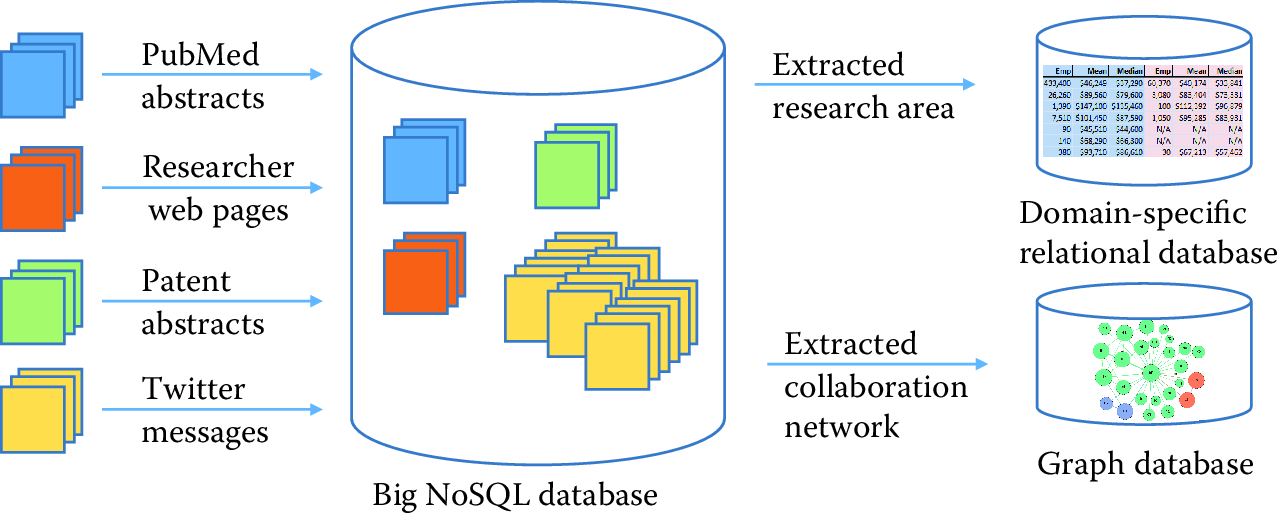
\includegraphics[width=0.7\linewidth]{ChapterDB/figures/data-fig2} 

}

\caption{A research project may use a NoSQL database to accumulate large amounts of data from many different sources, and then extract selected subsets to a relational or other database for more structured processing}\label{fig:figdb-dbs}
\end{figure}

\section{Relational DBMSs}\label{relational-dbmss}

We now provide a more detailed description of relational DBMSs.
Relational DBMSs implement the relational data model, in which data are
represented as sets of records organized in tables. This model is
particularly well suited for the structured data with which we
frequently deal in the social sciences; we discuss in Section
\protect\hyperlink{sec:db:nosql}{NoSQL databases} alternative data
models, such as those used in NoSQL databases.

We use the data shown in Figure \ref{fig:figdb-1} to introduce key
concepts. These two CSV format files describe grants made by the US
National Science Foundation (NSF). One file contains information about
grants, the other information about investigators. How should you
proceed to manipulate and analyze these data?

\begin{figure}

{\centering 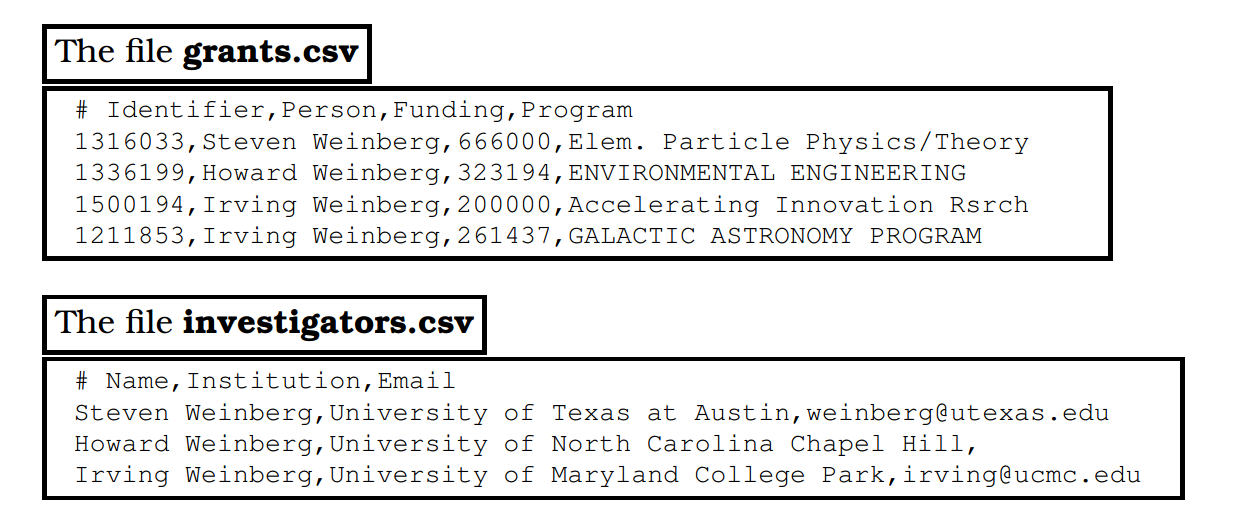
\includegraphics[width=0.7\linewidth]{ChapterDB/figures/figdb-1} 

}

\caption{CSV files representing grants and investigators. Each line in the first table specifies a grant number, investigator name, total funding amount, and NSF program name; each line in the second gives an investigator name, institution name, and investigator email address}\label{fig:figdb-1}
\end{figure}

The main concept underlying the relational data model is a \emph{table}
(also referred to as a \emph{relation}): a set of rows (also referred to
as tuples, records, or observations), each with the same columns (also
referred to as fields, attributes or variables). A database consists of
multiple tables. For example, we show in Figure \ref{fig:figdb-2} how
the data contained in the two CSV files of Figure \ref{fig:figdb-1} may
be represented as two tables. The \texttt{Grants} table contains one
tuple for each row in grants.csv, with columns \texttt{GrantID},
\texttt{Person}, \texttt{Funding}, and \texttt{Program}. The table
contains one tuple for each row in investigators.csv, with columns
\texttt{ID}, \texttt{Name}, \texttt{Institution}, and \texttt{Email}.
The CSV files and tables contain essentially the same information,
albeit with important differences (the addition of an \texttt{ID} field
in the \texttt{Investigators} table, the substitution of an \texttt{ID}
column for the \texttt{Person} column in the \texttt{Grants} table) that
we will explain below.

The use of the relational data model provides for physical independence:
a given table can be stored in many different ways. SQL queries are sets
of instructions to execute commands written in terms of the logical
representation of tables (i.e., their schema definition). Consequently,
even if the physical organization of the data changes (e.g., a different
layout is used to store the data on disk, or a new index is created to
speed up access for some queries), the queries need not change. Another
advantage of the relational data model is that, since a table is a
\emph{set}, in a mathematical sense, simple and intuitive set operations
(e.g., union, intersection) can be used to manipulate the data, as we
discuss below. We can easily, for example, determine the intersection of
two relations (e.g., grants that are awarded to a specific institution),
as we describe in the following. The database further ensures that the
data comply with the model (e.g., data types, key uniqueness, entity
relationships), essentially providing core quality assurance.

\begin{figure}

{\centering 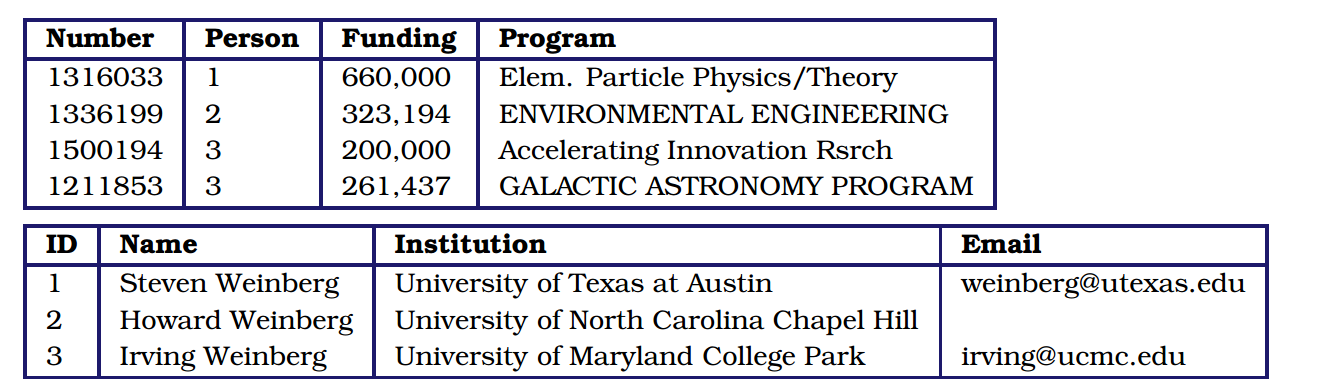
\includegraphics[width=0.7\linewidth]{ChapterDB/figures/figdb-2} 

}

\caption{Relational tables `Grants` and `Investigators` corresponding to the grants.csv and investigators.csv data in Figure 4.2, respectively. The only differences are the representation in a tabular form, the introduction of a unique numerical investigator identifier (`ID`) in the `Investigators` table, and the substitution of that identifier for the investigator name in the `Grants` table}\label{fig:figdb-2}
\end{figure}

\subsection{Structured Query Language
(SQL)}\label{structured-query-language-sql}

We use query languages to manipulate data in a database (e.g., to add,
update, or delete data elements) and to retrieve (raw and aggregated)
data from a database (e.g., data elements that certain properties). Most
Relational DBMSs support SQL, a simple, powerful query language with a
strong formal foundation based on logic, a foundation that allows
relational DBMSs to perform a wide variety of sophisticated
optimizations. SQL is used for three main purposes:

\begin{itemize}
\item
  \textbf{Data definition}: e.g., creation of new tables,
\item
  \textbf{Data manipulation}: queries and updates,
\item
  \textbf{Control}: creation of assertions to protect data integrity.
\end{itemize}

We introduce each of these features in the following, although not in
that order, and certainly not completely. Our goal here is to give
enough information to provide the reader with insights into how
relational databases work and what they do well; an in-depth SQL
tutorial is beyond the scope of this book, but we highly recommend
checking the references at the end of this chapter.

\hypertarget{sec:db:sql}{\subsection{Manipulating and querying
data}\label{sec:db:sql}}

SQL and other query languages used in DBMSs support the concise,
declarative specification of complex queries. Because we are eager to
show you something immediately useful, we cover these features first,
before talking about how to define data models.

\begin{center}\rule{0.5\linewidth}{\linethickness}\end{center}

\textbf{Example: Identifying grants of more than \$200,000} Here is an
SQL query to identify all grants with total funding of at most
\$200,000:

\begin{Shaded}
\begin{Highlighting}[]
\KeywordTok{select}\NormalTok{ * }\KeywordTok{from}\NormalTok{ Grants}
\KeywordTok{where}\NormalTok{ Funding <= }\DecValTok{200}\NormalTok{,}\DecValTok{000}\NormalTok{;}
\end{Highlighting}
\end{Shaded}

Notice SQL's declarative nature: this query can be read almost as the
English language statement, ``select all rows from the \texttt{Grants}
table for which the \texttt{Funding} column has value less than or equal
200,000.'' This query is evaluated as follows:

\begin{enumerate}
\def\labelenumi{\arabic{enumi}.}
\item
  The input table specified by the \texttt{from} clause,
  \texttt{Grants}, is selected.
\item
  The condition in the \texttt{where} clause,
  \texttt{Funding\ \textless{}=\ 200,000}, is checked against all rows
  in the input table to identify those rows that match.
\item
  The \texttt{select} clause specifies which columns to keep from the
  matching rows, that is, which columns constitute the schema of the
  output table. (The ``*'' indicates that all columns should be kept.)
\end{enumerate}

The answer, given the data in Figure \ref{fig:figdb-2}, is the following
single-row table. (The fact that an SQL query returns a table is
important when it comes to creating more complex queries: the result of
a query can be stored into the database as a new table, or passed to
another query as input.)

\begin{longtable}[]{@{}llll@{}}
\toprule
\textbf{Number} & \textbf{Person} & \textbf{Funding} &
\textbf{Program}\tabularnewline
\midrule
\endhead
1500194 & 3 & 200,000 & Accelerating Innovation Rsrch\tabularnewline
\bottomrule
\end{longtable}

\begin{center}\rule{0.5\linewidth}{\linethickness}\end{center}

DBMSs automatically optimize declarative queries such as the example
that we just presented, translating them into a set of low-level data
manipulations (an imperative \emph{query plan}) that can be evaluated
efficiently. This feature allows users to write queries without having
to worry too much about performance issues---the database does the
worrying for you. For example, a DBMS need not consider every row in the
\texttt{Grants} table in order to identify those with funding less than
\$200,000, a strategy that would be slow if the \texttt{Grants} table
were large: it can instead use an index to retrieve the relevant records
much more quickly. We discuss indices in more detail in Section
\protect\hyperlink{sec:db:index}{Database optimizations}.

The querying component of SQL supports a wide variety of manipulations
on tables, whether referred to explicitly by a table name (as in the
example just shown) or constructed by another query. We just saw how to
use the \texttt{select} operator to both pick certain rows (what is
termed \emph{selection}) and certain columns (what is called
\emph{projection}) from a table.

\begin{center}\rule{0.5\linewidth}{\linethickness}\end{center}

\textbf{Example: Finding grants awarded to an investigator}

We want to find all grants awarded to the investigator with name
``Irving Weinberg.'' The information required to answer this question is
distributed over two tables, \texttt{Grants} and \texttt{Investigators},
and so we \emph{join} the two tables to combine tuples from both:

\begin{Shaded}
\begin{Highlighting}[]
\KeywordTok{select} \DataTypeTok{Number}\NormalTok{, Name, Funding, Program}
\KeywordTok{from}\NormalTok{ Grants, Investigators}
\KeywordTok{where}\NormalTok{ Grants.Person = Investigators.ID}
\KeywordTok{and}\NormalTok{ Name = }\OtherTok{"Irving Weinberg"}\NormalTok{;}
\end{Highlighting}
\end{Shaded}

This query combines tuples from the \texttt{Grants} and
\texttt{Investigators} tables for which the \texttt{Person} and
\texttt{ID} fields match. It is evaluated in a similar fashion to the
query presented above, except for the \texttt{from} clause: when
multiple tables are listed, as here, the conditions in the
\texttt{where} clause are checked for all different combinations of
tuples from the tables defined in the \texttt{from} clause (i.e., the
cartesian product of these tables)---in this case, a total of
\(3\times 4 = 12\) combinations. We thus determine that Irving Weinberg
has two grants. The query further selects the \texttt{Number},
\texttt{Name}, \texttt{Funding}, and \texttt{Program} fields from the
result, giving the following:

\begin{longtable}[]{@{}llll@{}}
\toprule
\textbf{Number} & \textbf{Person} & \textbf{Funding} &
\textbf{Program}\tabularnewline
\midrule
\endhead
1500194 & Irving Weinberg & 200,000 & Accelerating Innovation
Rsrch\tabularnewline
1211853 & Irving Weinberg & 261,437 & GALACTIC ASTRONOMY
PROGRAM\tabularnewline
\bottomrule
\end{longtable}

This ability to join two tables in a query is one example of how SQL
permits concise specifications of complex computations. This joining of
tables via a cartesian product operation is formally called a
\emph{cross join}. Other types of join are also supported. We describe
one such, the \emph{inner join}, in Section
\protect\hyperlink{sec:db:spatial}{Spatial databases}.

\begin{center}\rule{0.5\linewidth}{\linethickness}\end{center}

SQL aggregate functions allow for the computation of aggregate
statistics over tables. For example, we can use the following query to
determine the total number of grants and their total and average funding
levels:

\begin{Shaded}
\begin{Highlighting}[]
\KeywordTok{select} \FunctionTok{count}\NormalTok{(*) }\KeywordTok{as} \StringTok{'Number'}\NormalTok{, }\FunctionTok{sum}\NormalTok{(Funding) }\KeywordTok{as} \StringTok{'Total'}\NormalTok{,}
       \FunctionTok{avg}\NormalTok{(Funding) }\KeywordTok{as} \StringTok{'Average'}
\KeywordTok{from}\NormalTok{ Grants;}
\end{Highlighting}
\end{Shaded}

This yields the following:

\begin{longtable}[]{@{}lll@{}}
\toprule
\textbf{Number} & \textbf{Total} & \textbf{Average}\tabularnewline
\midrule
\endhead
4 & 1444631 & 361158\tabularnewline
\bottomrule
\end{longtable}

The \texttt{group\ by} operator can be used in conjunction with the
aggregate functions to group the result set by one or more columns. For
example, we can use the following query to create a table with three
columns: investigator name, the number of grants associated with the
investigator, and the aggregate funding:

\begin{Shaded}
\begin{Highlighting}[]
\KeywordTok{select}\NormalTok{ Name, }\FunctionTok{count}\NormalTok{(*) }\KeywordTok{as} \StringTok{'Number'}\NormalTok{,}
       \FunctionTok{avg}\NormalTok{(Funding) }\KeywordTok{as} \StringTok{'Average funding'}
\KeywordTok{from}\NormalTok{ Grants, Investigators}
\KeywordTok{where}\NormalTok{ Grants.Person = Investigators.ID}
\KeywordTok{group} \KeywordTok{by}\NormalTok{ Name;}
\end{Highlighting}
\end{Shaded}

We obtain the following:

\begin{longtable}[]{@{}lll@{}}
\toprule
\textbf{Name} & \textbf{Number} & \textbf{Average
Funding}\tabularnewline
\midrule
\endhead
Steven Weinberg & 1 & 666000\tabularnewline
Howard Weinberg & 1 & 323194\tabularnewline
Irving Weinberg & 2 & 230719\tabularnewline
\bottomrule
\end{longtable}

\hypertarget{sec:db:schema}{\subsection{Schema design and
definition}\label{sec:db:schema}}

\begin{figure}

{\centering 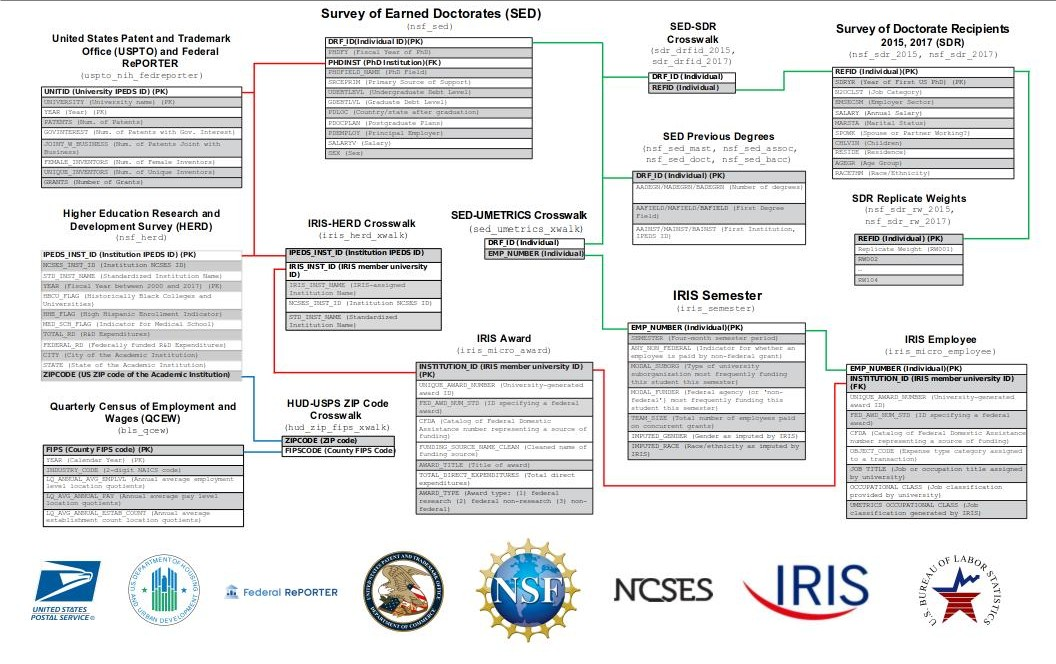
\includegraphics[width=0.7\linewidth]{ChapterDB/figures/NCSES-Database-Diagram} 

}

\caption{A database schema can show the ways in which many tables are linked. Here, there are individual-links (shown in green) as well as institution-level links (shown in red) and location-level links (shown in blue).}\label{fig:NCSES}
\end{figure}

When using a pre-existing database, you will be given the database
design that includes tables, rows, and columns. But, when you are
starting with your own data and need to create a database, the first
step is to come up with the design of the database.

We have seen that a relational database comprises a set of tables. The
task of specifying the structure of the data to be stored in a database
is called \emph{logical design}. This task may be performed by a
database administrator, in the case of a database to be shared by many
people, or directly by users, if they are creating databases themselves.
More specifically, the logical design process involves defining a
\emph{schema}. A schema comprises a set of tables (including, for each
table, its columns and their types), their relationships, and integrity
constraints.

The first step in the logical design process is to identify the entities
that need to be modeled. In our example, we identified two important
classes of entity: ``grants'' and ``investigators.'' We thus define a
table for each; each row in these two tables will correspond to a unique
grant or investigator, respectively. (In a more complete and realistic
design, we would likely also identify other entities, such as
institutions and research products.) During this step, we will often
find ourselves breaking information up into multiple tables, so as to
avoid duplicating information.

For example, imagine that we were provided grant information in the form
of one CSV file rather than two, with each line providing a grant
number, investigator, funding, program, institution, and email. In this
file, the name, institution, and email address for Irving Weinberg would
then appear twice, as he has two grants, which can lead to errors when
updating values and make it difficult to represent certain information.
(For example, if we want to add an investigator who does not yet have a
grant, we will need to create a tuple (row) with empty slots for all
columns (variables) associated with grants.) Thus we would want to break
up the single big table into the two tables that we defined here. This
breaking up of information across different tables to avoid repetition
of information is referred to as \textbf{normalization}.\footnote{Normalization
  involves organizing columns and tables of a relational database to
  minimize data redundancy.}\footnote{Normalization can be done in
  statistical packages as well. For example, as noted above, PSID splits
  its data into different files linked through ID variables. The
  difference here is that the DBMS makes creating, navigating, and
  querying the resulting data particularly easy.}

The second step in the design process is to define the columns that are
to be associated with each entity. For each table, we define a set of
columns. For example, given the data in Figure \ref{fig:figdb-1}, the
grant table should include columns for award identifier, title,
investigator, and award amount; for an investigator, the columns will be
name, university, and email address. In general, we will want to ensure
that each row in our table has a key: a set of columns that uniquely
identifies that row. In our example tables, grants are uniquely
identified by \texttt{Number} and investigators by \texttt{ID}.

The third step in the design process is to capture relationships between
entities. In our example, we are concerned with just one relationship,
namely that between grants and investigators: each grant has an
investigator. We represent this relationship between tables by
introducing a \texttt{Person} column in the \texttt{Grants} table, as
shown in Figure \ref{fig:figdb-2}. Note that we do not simply duplicate
the investigator names in the two tables, as was the case in the two CSV
files shown in Figure \ref{fig:figdb-1}: these names might not be
unique, and the duplication of data across tables can lead to later
inconsistencies if a name is updated in one table but not the other.

The final step in the design process is to represent integrity
constraints (or rules) that must hold for the data. In our example, we
may want to specify that each grant must be awarded to an investigator;
that each value of the grant identifier column must be unique (i.e.,
there cannot be two grants with the same number); and that total funding
can never be negative. Such restrictions can be achieved by specifying
appropriate constraints at the time of schema creation, as we show in
Listing \protect\hyperlink{list:db1}{Grantdata}, which contains the code
used to create the two tables that make up our schema.

Listing \protect\hyperlink{list:db1}{Grantdata} contains four SQL
statements. The first two statements, lines 1 and 2, simply set up our
new database. The \texttt{create\ table} statement in lines 1 and 2
creates our first table. It specifies the table name
(\texttt{Investigators}) and, for each of the four columns, the column
name and its type.\footnote{These storage types will be familiar to many
  of you from statistical software packages.} Relational DBMSs offer a
rich set of types to choose from when designing a table: for example,
\texttt{int} or \texttt{integer} (synonyms); \texttt{real} or
\texttt{float}(synonyms); \texttt{char(n)}, a fixed-length string of
\texttt{n} characters; and \texttt{varchar(n)}, a variable-length string
of up to \texttt{n} characters. Types are important for several reasons.
First, they allow for more efficient encoding of data. For example, the
\texttt{Funding} field in the grants.csv file of Figure
\ref{fig:figdb-1} could be represented as a string in the
\texttt{Grants} table, \texttt{char(15)}, say, to allow for large
grants. By representing it as a floating point number instead (line 15
in Listing \protect\hyperlink{list:db1}{Grantdata}), we reduce the space
requirement per grant to just four bytes. Second, types allow for
integrity checks on data as they are added to the database: for example,
that same type declaration for \texttt{Funding} ensures that only valid
numbers will be entered into the database. Third, types allow for
type-specific operations on data, such as arithmetic operations on
numbers (e.g., min, max, sum).

Other SQL features allow for the specification of additional constraints
on the values that can be placed in the corresponding column. For
example, the \texttt{not\ null} constraints for \texttt{Name} and
\texttt{Institution} (lines 6, 7) indicate that each investigator must
have a name and an institution, respectively. (The lack of such a
constraint on the \texttt{Email} column shows that an investigator need
not have an email address.)

\begin{Shaded}
\begin{Highlighting}[]
\KeywordTok{create} \KeywordTok{database}\NormalTok{ grantdata;}
\KeywordTok{use}\NormalTok{ grantdata;}

\KeywordTok{create} \KeywordTok{table}\NormalTok{ Investigators (}
    \KeywordTok{ID} \DataTypeTok{int}\NormalTok{ auto_increment,}
\NormalTok{    Name }\DataTypeTok{varchar}\NormalTok{(}\DecValTok{100}\NormalTok{) }\KeywordTok{not} \KeywordTok{null}\NormalTok{,}
\NormalTok{    Institution }\DataTypeTok{varchar}\NormalTok{(}\DecValTok{256}\NormalTok{) }\KeywordTok{not} \KeywordTok{null}\NormalTok{,}
\NormalTok{    Email }\DataTypeTok{varchar}\NormalTok{(}\DecValTok{100}\NormalTok{),}
    \KeywordTok{primary} \KeywordTok{key}\NormalTok{(}\KeywordTok{ID}\NormalTok{)}
\NormalTok{);}

\KeywordTok{create} \KeywordTok{table}\NormalTok{ Grants ( }
    \DataTypeTok{Number} \DataTypeTok{int} \KeywordTok{not} \KeywordTok{null}\NormalTok{,}
\NormalTok{    Person }\DataTypeTok{int} \KeywordTok{not} \KeywordTok{null}\NormalTok{,}
\NormalTok{    Funding }\DataTypeTok{float}\NormalTok{ unsigned }\KeywordTok{not} \KeywordTok{null}\NormalTok{,}
\NormalTok{    Program }\DataTypeTok{varchar}\NormalTok{(}\DecValTok{100}\NormalTok{),}
    \KeywordTok{primary} \KeywordTok{key}\NormalTok{(}\DataTypeTok{Number}\NormalTok{)}
\NormalTok{);}
\end{Highlighting}
\end{Shaded}

Listing: Code to create the grantdata database and its Investigators and
Grants tables

\subsection{Loading data}\label{loading-data}

So far we have created a database and two empty tables. The next step is
to add data to the tables. We can of course do that manually, row by
row, but in most cases we will import data from another source, such as
a CSV file. Listing \protect\hyperlink{list:db2}{Load data} shows the
two statements that load the data of Figure \ref{fig:figdb-1} into our
two tables. (Here and elsewhere in this chapter, we use the MySQL DBMS.
The SQL syntax used by different DBMSs differs in various, mostly minor
ways.) Each statement specifies the name of the file from which data is
to be read and the table into which it is to be loaded. The
\texttt{fields\ terminated\ by\ ","} statement tells SQL that values are
separated by columns, and \texttt{ignore\ 1\ lines} tells SQL to skip
the header. The list of column names is used to specify how values from
the file are to be assigned to columns in the table.

For the \texttt{Investigators} table, the three values in each row of
the investigators.csv file are assigned to the \texttt{Name},
\texttt{Institution}, and \texttt{Email} columns of the corresponding
database row. Importantly, the \texttt{auto\_increment} declaration on
the \texttt{ID} column (line 5 in Listing
\protect\hyperlink{list:db1}{Grantdata}) causes values for this column
to be assigned automatically by the DBMS, as rows are created, starting
at \texttt{1}. This feature allows us to assign a unique integer
identifier to each investigator as its data are loaded.

\begin{Shaded}
\begin{Highlighting}[]
\NormalTok{load }\KeywordTok{data} \KeywordTok{local}\NormalTok{ infile }\OtherTok{"investigators.csv"}
    \KeywordTok{into} \KeywordTok{table}\NormalTok{ Investigators}
\NormalTok{    fields terminated }\KeywordTok{by} \OtherTok{","}
\NormalTok{    ignore }\DecValTok{1}\NormalTok{ lines}
\NormalTok{    (Name, Institution, Email);}

\NormalTok{load }\KeywordTok{data} \KeywordTok{local}\NormalTok{ infile }\OtherTok{"grants.csv"} \KeywordTok{into} \KeywordTok{table}\NormalTok{ Grants}
\NormalTok{    fields terminated }\KeywordTok{by} \OtherTok{","}
\NormalTok{    ignore }\DecValTok{1}\NormalTok{ lines}
\NormalTok{    (}\DataTypeTok{Number}\NormalTok{, @var, Funding, Program)}
\KeywordTok{set}\NormalTok{ Person = (}\KeywordTok{select} \KeywordTok{ID} \KeywordTok{from}\NormalTok{ Investigators}
              \KeywordTok{where}\NormalTok{ Investigators.Name=@var);}
\end{Highlighting}
\end{Shaded}

Listing: Code to load data into the Investigators and Grants tables

For the \texttt{Grants} table, the \texttt{load\ data} call (lines
7--12) is somewhat more complex. Rather than loading the investigator
name (the second column of each line in our data file, represented here
by the variable \texttt{@var}) directly into the database, we use an SQL
query (the \texttt{select} statement in lines 11--12) to retrieve from
the \texttt{Investigators} table the \texttt{ID} corresponding to that
name. By thus replacing the investigator name with the unique
investigator identifier, we avoid replicating the name across the two
tables.

\subsection{Transactions and crash
recovery}\label{transactions-and-crash-recovery}

A DBMS protects the data that it stores from computer crashes: if your
computer stops running suddenly (e.g., your operating system crashes or
you unplug the power), the contents of your database are not corrupted.
It does so by supporting \emph{transactions}. A transaction is an atomic
sequence of database actions. In general, every SQL statement is
executed as a transaction. You can also specify sets of statements to be
combined into a single transaction, but we do not cover that capability
here. The DBMS ensures that each transaction is executed completely even
in the case of failure or error: if the transaction succeeds, the
results of all operations are recorded permanently (``persisted'') in
the database, and if it fails, all operations are ``rolled back'' and no
changes are committed. For example, suppose we ran the following SQL
statement to convert the funding amounts in the table from dollars to
euros, by scaling each number by 0.9. The \texttt{update} statement
specifies the table to be updated and the operation to be performed,
which in this case is to update the \texttt{Funding} column of each row.
The DBMS will ensure that either no rows are altered or all are altered.

\begin{Shaded}
\begin{Highlighting}[]
\KeywordTok{update}\NormalTok{ Grants }\KeywordTok{set}\NormalTok{ Grants.Funding = Grants.Funding*}\FloatTok{0.9}\NormalTok{;}
\end{Highlighting}
\end{Shaded}

Transactions are also key to supporting multi-user access. The
\emph{concurrency control} mechanisms in a DBMS allow multiple users to
operate on a database concurrently, as if they were the only users of
the system: transactions from multiple users can be interleaved to
ensure fast response times, while the DBMS ensures that the database
remains consistent. While entire books could be (and have been) written
on concurrency in databases, the key point is that read operations can
proceed concurrently, while update operations are typically serialized.

\hypertarget{sec:db:index}{\subsection{Database
optimizations}\label{sec:db:index}}

A relational DBMS applies query planning and optimization methods with
the goal of evaluating queries as efficiently as possible. For example,
if a query asks for rows that fit two conditions, one cheap to evaluate
and one expensive, a relational DBMS may filter first on the basis of
the first condition, and then apply the second conditions only to the
rows identified by that first filter. These sorts of optimization are
what distinguish SQL from other programming languages, as they allow the
user to write queries declaratively and rely on the DBMS to come up with
an efficient execution strategy.

Nevertheless, the user can help the DBMS to improve performance. The
single most powerful performance improvement tool is the index, an
internal data structure that the DBMS maintains to speed up queries.
While various types of indices can be created, with different
characteristics, the basic idea is simple. Consider the column in our
table. Assume that there are \(N\) rows in the table. In the absence of
an index, a query that refers to a column value (e.g.,
\texttt{where\ ID=3}) would require a linear scan of the table, taking
on average \(N/2\) comparisons and in the worst case \(N\) comparisons.
A binary tree index allows the desired value to be found with just
\(\log_2 N\) comparisons.

\begin{center}\rule{0.5\linewidth}{\linethickness}\end{center}

\textbf{Example: Using indices to improve database performance}

Consider the following query:

\begin{Shaded}
\begin{Highlighting}[]
\KeywordTok{select} \KeywordTok{ID}\NormalTok{, Name, }\FunctionTok{sum}\NormalTok{(Funding) }\KeywordTok{as}\NormalTok{ TotalFunding}
  \KeywordTok{from}\NormalTok{ Grants, Investigators}
    \KeywordTok{where}\NormalTok{ Investigators.ID=Grants.Person}
  \KeywordTok{group} \KeywordTok{by} \KeywordTok{ID}\NormalTok{;}
\end{Highlighting}
\end{Shaded}

This query joins our two tables to link investigators with the grants
that they hold, groups grants by investigator (using
\texttt{group\ by}), and finally sums the funding associated with the
grants held by each investigator. The result is the following:

\begin{longtable}[]{@{}lll@{}}
\toprule
\textbf{ID} & \textbf{Name} & \textbf{TotalFunding}\tabularnewline
\midrule
\endhead
1 & Steven Weinberg & 666000\tabularnewline
2 & Howard Weinberg & 323194\tabularnewline
3 & Irving Weinberg & 230719\tabularnewline
\bottomrule
\end{longtable}

In the absence of indices, the DBMS must compare each row in
\texttt{Investigators} with each row in \texttt{Grants}, checking for
each pair whether \texttt{Investigators.ID\ =\ Grants.Person} holds. As
the two tables in our sample database have only three and four rows,
respectively, the total number of comparisons is only \(3\times 4=12\).
But if we had, say, 1 million investigators and 1 million grants, then
the DBMS would have to perform 1 trillion comparisons, which would take
a long time. (More importantly, it would have to perform a large number
of disk I/O operations, if the tables did not fit in memory.) An index
on the \texttt{ID} column of the \texttt{Investigators} table reduces
the number of operations dramatically, as the DBMS can then take each of
the 1 million rows in the \texttt{Grants} table and, for each row,
identify the matching row(s) in \texttt{Investigators} via an index
lookup rather than a linear scan.

In our example table, the \texttt{ID} column has been specified to be a
\texttt{primary\ key}, and thus an index is created for it
automatically. If it were not, we could easily create the desired index
as follows:

\begin{Shaded}
\begin{Highlighting}[]
\KeywordTok{alter} \KeywordTok{table}\NormalTok{ Investigators }\KeywordTok{add} \KeywordTok{index}\NormalTok{(}\KeywordTok{ID}\NormalTok{);}
\end{Highlighting}
\end{Shaded}

It can be difficult for the user to determine when an index is required.
A good rule of thumb is to create an index for any column that is
queried often, that is, appears on the right-hand side of a
\texttt{where} statement that is to be evaluated frequently. However,
the presence of indices makes updates more expensive, as every change to
a column value requires that the index be rebuilt to reflect the change.
Thus, if your data are highly dynamic, you should carefully select which
indices to create. (For bulk load operations, a common practice is to
drop indices prior to the data import, and re-create them once the load
is completed.) Also, indices take disk space, so you need to consider
the tradeoff between query efficiency and resources.

The \texttt{explain} command can be useful for determining when indices
are required. For example, we show in the following some of the output
produced when we apply \texttt{explain} to our query. (For this example,
we have expanded the two tables to 1,000 rows each, as our original
tables are too small for MySQL to consider the use of indices.) The
output provides useful information such as the key(s) that could be
used, if indices exist (\texttt{Person} in the \texttt{Grants} table,
and the primary key, \texttt{ID}, for the \texttt{Investigators} table);
the key(s) that are actually used (the primary key, \texttt{ID}, in the
\texttt{Investigators} table); the column(s) that are compared to the
index (\texttt{Investigators.ID} is compared with
\texttt{Grants.Person}); and the number of rows that must be considered
(each of the 1,000 rows in \texttt{Grants} is compared with one row in
\texttt{Investigators}, for a total of 1,000 comparisons).

\begin{Shaded}
\begin{Highlighting}[]
\NormalTok{mysql> }\KeywordTok{explain} \KeywordTok{select} \KeywordTok{ID}\NormalTok{, Name, }\FunctionTok{sum}\NormalTok{(Funding) }\KeywordTok{as}\NormalTok{ TotalFunding}
       \KeywordTok{from}\NormalTok{ Grants, Investigators}
       \KeywordTok{where}\NormalTok{ Investigators.ID=Grants.Person }\KeywordTok{group} \KeywordTok{by} \KeywordTok{ID}\NormalTok{;}

\NormalTok{+}\CommentTok{---------------+---------------+---------+---------------+------+}
\NormalTok{| }\KeywordTok{table}\NormalTok{         | possible_keys | }\KeywordTok{key}\NormalTok{     | }\FunctionTok{ref}\NormalTok{           | }\KeywordTok{rows}\NormalTok{ |}
\NormalTok{+}\CommentTok{---------------+---------------+---------+---------------+------+}
\NormalTok{| Grants        | Person        | }\KeywordTok{NULL}\NormalTok{    | }\KeywordTok{NULL}\NormalTok{          | }\DecValTok{1000}\NormalTok{ |}
\NormalTok{| Investigators | }\KeywordTok{PRIMARY}\NormalTok{       | }\KeywordTok{PRIMARY}\NormalTok{ | Grants.Person |    }\DecValTok{1}\NormalTok{ |}
\NormalTok{+}\CommentTok{---------------+---------------+---------+---------------+------+}
\end{Highlighting}
\end{Shaded}

Contrast this output with the output obtained for equivalent tables in
which is not a primary key. In this case, no keys are used and thus
\(1{,}000\times 1{,}000=1{,}000{,}000\) comparisons, and the associated
disk reads, must be performed.

\begin{Shaded}
\begin{Highlighting}[]
\NormalTok{+}\CommentTok{---------------+---------------+------+------+------+}
\NormalTok{| }\KeywordTok{table}\NormalTok{         | possible_keys | }\KeywordTok{key}\NormalTok{  | }\FunctionTok{ref}\NormalTok{  | }\KeywordTok{rows}\NormalTok{ |}
\NormalTok{+}\CommentTok{---------------+---------------+------+------+------+}
\NormalTok{| Grants        | Person        | }\KeywordTok{NULL}\NormalTok{ | }\KeywordTok{NULL}\NormalTok{ | }\DecValTok{1000}\NormalTok{ |}
\NormalTok{| Investigators | }\KeywordTok{ID}\NormalTok{            | }\KeywordTok{NULL}\NormalTok{ | }\KeywordTok{NULL}\NormalTok{ | }\DecValTok{1000}\NormalTok{ |}
\NormalTok{+}\CommentTok{---------------+---------------+------+------+------+}
\end{Highlighting}
\end{Shaded}

\begin{center}\rule{0.5\linewidth}{\linethickness}\end{center}

A second way in which the user can contribute to performance improvement
is by using appropriate table definitions and data types. Most DBMSs
store data on disk. Data must be read from disk into memory before it
can be manipulated. Memory accesses are fast, but loading data into
memory is expensive: accesses to main memory can be a million times
faster than accesses to disk. Therefore, to ensure queries are
efficient, it is important to minimize the number of disk accesses. A
relational DBMS automatically optimizes queries: based on how the data
are stored, it transforms a SQL query into a query plan that can be
executed efficiently, and chooses an execution strategy that minimizes
disk accesses. But users can contribute to making queries efficient. As
discussed above, the choice of types made when defining schemas can make
a big difference. As a rule of thumb, only use as much space as needed
for your data: the smaller your records, the more records can be
transferred to main memory using a single disk access. The design of
relational tables is also important. If you put all columns in a single
table (i.e., you do not normalize), more data may come into memory than
is required.

\subsection{Caveats and challenges}\label{caveats-and-challenges}

It is important to keep the following caveats and challenges in mind
when using SQL technology with social science data.

\textbf{Data cleaning}

Data created outside an SQL database, such as data in files, are not
always subject to strict constraints: data types may not be correct or
consistent (e.g., numeric data stored as text) and consistency or
integrity may not be enforced (e.g., absence of primary keys, missing
foreign keys). Indeed, as the reader probably knows well from
experience, data are rarely perfect. As a result, the data may fail to
comply with strict SQL schema requirements and fail to load, in which
case either data must be cleaned before or during loading, or the SQL
schema must be relaxed.

\textbf{Missing values}

Care must be taken when loading data in which some values may be missing
or blank. SQL engines represent and refer to a missing or blank value as
the built-in constant \texttt{null}. Counterintuitively, when loading
data from text files (e.g., CSV), many SQL engines require that missing
values be represented explicitly by the term \texttt{null}; if a data
value is simply omitted, it may fail to load or be incorrectly
represented, for example as zero or the empty string (\texttt{""})
instead of \texttt{null}. Thus, for example, the second row in the
investigators.csv file of Figure \ref{fig:figdb-1}:

\texttt{Howard\ Weinberg,University\ of\ North\ Carolina\ Chapel\ Hill,}

may need to be rewritten as:

\texttt{Howard\ Weinberg,University\ of\ North\ Carolina\ Chapel\ Hill,null}

\textbf{Metadata for categorical variables}

SQL engines are metadata poor: they do not allow extra information to be
stored about a variable (field) beyond its base name and type
(\texttt{int}, \texttt{char}, etc., as introduced in Section
\protect\hyperlink{sec:db:schema}{Schema design and definition}). They
cannot, for example, record directly the fact that the column
\texttt{class} can only take one of three values, \texttt{animal},
\texttt{vegetable}, or \texttt{mineral}, or what these values mean.
Common practice is thus to store information about possible values in
another table (commonly referred to as a \emph{dimension table}) that
can be used as a lookup and constraint, as in the following:

Table \textbf{class\_values}

\begin{longtable}[]{@{}ll@{}}
\toprule
\textbf{Value} & \textbf{Description}\tabularnewline
\midrule
\endhead
\texttt{animal} & Is alive\tabularnewline
\texttt{vegetable} & Grows\tabularnewline
\texttt{mineral} & Isn't alive and doesn't grow\tabularnewline
\bottomrule
\end{longtable}

A related concept is that a column or list of columns may be declared
\texttt{primary\ key} or \texttt{unique}. Such a statement specifies
that no two tuples of the table may agree in the specified column---or,
if a list if columns is provided, in all of those columns. There can be
only one \texttt{primary\ key} for a table, but several \texttt{unique}
columns. No column of a \texttt{primary\ key} can ever be \texttt{null}
in any tuple. But columns declared \texttt{unique} may have
\texttt{null}s, and there may be several tuples with \texttt{null}.

\section{Linking DBMSs and other
tools}\label{linking-dbmss-and-other-tools}

Query languages such as SQL are not general-purpose programming
languages; they support easy, efficient access to large data sets, are
extremely efficient for specific types of analysis, but may not be the
right choice for all analysis. When complex computations are required,
one can embed query language statements into a programming language or
statistical package. For example, we might want to calculate the
interquartile range of funding for all grants. While this calculation
can be accomplished in SQL, the resulting SQL code will be complicated
(depending on which flavor of SQL your database supports). Languages
like Python make such statistical calculations straightforward, so it is
natural to write a Python (or R, SAS, Stata, etc.) program that connects
to the DBMS that contains our data, fetches the required data from the
DBMS, and then calculates the interquartile range of those data. The
program can then, if desired, store the result of this calculation back
into the database.

Many relational DBMSs also have built-in analytical functions or often
now support different programming languages, providing significant
in-database statistical and analytical capabilities and alleviating the
need for external processing.

\begin{Shaded}
\begin{Highlighting}[]
\KeywordTok{from}\NormalTok{ mysql.connector import MySQLConnection, Error}
\KeywordTok{from}\NormalTok{ python_mysql_dbconfig import read_db_config}

\NormalTok{def retrieve_and_analyze_data():}
\NormalTok{    try:}
\NormalTok{        # }\KeywordTok{Open}\NormalTok{ connection }\KeywordTok{to} \KeywordTok{the}\NormalTok{ MySQL }\KeywordTok{database}
\NormalTok{        dbconfig = read_db_config()}
\NormalTok{        conn = MySQLConnection(**dbconfig)}
        \KeywordTok{cursor}\NormalTok{ = conn.cursor()}
\NormalTok{        # Transmit }\KeywordTok{the}\NormalTok{ SQL }\KeywordTok{query} \KeywordTok{to} \KeywordTok{the} \KeywordTok{database}
\NormalTok{        cursor.execute(}\StringTok{'select Funding from Grants;'}\NormalTok{)}
\NormalTok{        # Fetch }\KeywordTok{all} \KeywordTok{rows} \KeywordTok{of} \KeywordTok{the} \KeywordTok{query}\NormalTok{ response}
        \KeywordTok{rows}\NormalTok{ = [}\KeywordTok{row} \KeywordTok{for} \KeywordTok{row} \KeywordTok{in}\NormalTok{ cur.fetchall()]}
\NormalTok{        calculate_inter_quartile_range(}\KeywordTok{rows}\NormalTok{)}
    \KeywordTok{except}\NormalTok{ Error }\KeywordTok{as}\NormalTok{ e:}
\NormalTok{        print(e)}
\NormalTok{    finally:}
\NormalTok{        cursor.close()}
\NormalTok{        conn.close()}

\KeywordTok{if}\NormalTok{ __name__ == }\StringTok{'__main__'}\NormalTok{:}
\NormalTok{    retrieve_and_analyze_data()}
\end{Highlighting}
\end{Shaded}

Listing: Embedding SQL in Python

\begin{center}\rule{0.5\linewidth}{\linethickness}\end{center}

\textbf{Example: Embedding database queries in Python}

The Python script in Listing \protect\hyperlink{list:db3}{Embedding}
shows how this embedding of database queries in Python is done. This
script establishes a connection to the database, transmits the desired
SQL query to the database (line 7--9), retrieves the query results into
a Python array (line 11), and calls a Python procedure (not given) to
perform the desired computation (line 14). A similar program could be
used to load the results of a Python (or R, SAS, Stata, etc.)
computation into a database.

\begin{center}\rule{0.5\linewidth}{\linethickness}\end{center}

\begin{center}\rule{0.5\linewidth}{\linethickness}\end{center}

\textbf{Example: Loading other structured data}

We saw in Listing \protect\hyperlink{list:db2}{Load data} how to load
data from CSV files into SQL tables. Data in other formats, such as the
commonly used JSON, can also be loaded into a relational DBMS. Consider,
for example, the following JSON format data, a simplified version of
data shown in Chapter \protect\hyperlink{chap:web}{Working with Web Data
and APIs}.

\begin{Shaded}
\begin{Highlighting}[]
\NormalTok{[}
\NormalTok{  \{}
\NormalTok{    institute }\OperatorTok{:}\StringTok{ }\NormalTok{Janelia Campus,}
\NormalTok{    name }\OperatorTok{:}\StringTok{ }\NormalTok{Laurence Abbott,}
\NormalTok{    role }\OperatorTok{:}\StringTok{ }\NormalTok{Senior Fellow,}
\NormalTok{    state }\OperatorTok{:}\StringTok{ }\NormalTok{VA,}
\NormalTok{    town }\OperatorTok{:}\StringTok{ }\NormalTok{Ashburn}
\NormalTok{  \},}
\NormalTok{  \{}
\NormalTok{    institute }\OperatorTok{:}\StringTok{ }\NormalTok{Jackson Lab,}
\NormalTok{    name }\OperatorTok{:}\StringTok{ }\NormalTok{Susan Ackerman,}
\NormalTok{    role }\OperatorTok{:}\StringTok{ }\NormalTok{Investigator,}
\NormalTok{    state }\OperatorTok{:}\StringTok{ }\NormalTok{ME,}
\NormalTok{    town }\OperatorTok{:}\StringTok{ }\NormalTok{Bar Harbor}
\NormalTok{  \}}
\NormalTok{]}
\end{Highlighting}
\end{Shaded}

While some relational DBMSs (such as PostgresQL) provide built-in
support for JSON objects, we assume here that we want to convert these
data into normal SQL tables. Using one of the many utilities for
converting JSON into CSV, we can construct the following CSV file, which
we can load into an SQL table using the method shown earlier.

\begin{verbatim}
institute,name,role,state,town
Janelia Campus,Laurence Abbott,Senior Fellow,VA,Ashburn
Jackson Lab,Susan Ackerman,Investigator,ME,Bar Harbor
\end{verbatim}

But into what table? The two records each combine information about a
person with information about an institute. Following the schema design
rules given in Section \protect\hyperlink{sec:db:schema}{Schema design
and definition}, we should \emph{normalize} the data by reorganizing
them into two tables, one describing people and one describing
institutes. Similar problems arise when JSON documents contain nested
structures. For example, consider the following alternative JSON
representation of the data above. Here, the need for normalization is
yet more apparent.

\begin{Shaded}
\begin{Highlighting}[]
\NormalTok{[}
\NormalTok{  \{}
\NormalTok{    name }\OperatorTok{:}\StringTok{ }\NormalTok{Laurence Abbott,}
\NormalTok{    role }\OperatorTok{:}\StringTok{ }\NormalTok{Senior Fellow,}
\NormalTok{    employer }\OperatorTok{:}\StringTok{ }\NormalTok{\{ institute }\OperatorTok{:}\StringTok{ }\NormalTok{Janelia Campus,}
\NormalTok{                 state }\OperatorTok{:}\StringTok{ }\NormalTok{VA,}
\NormalTok{                 town }\OperatorTok{:}\StringTok{ }\NormalTok{Ashburn\}}
\NormalTok{  \},}
\NormalTok{  \{}
\NormalTok{    name }\OperatorTok{:}\StringTok{ }\NormalTok{Susan Ackerman,}
\NormalTok{    role }\OperatorTok{:}\StringTok{ }\NormalTok{Investigator,}
\NormalTok{    employer}\OperatorTok{:}\StringTok{ }\NormalTok{\{ institute }\OperatorTok{:}\StringTok{ }\NormalTok{Jackson Lab,}
\NormalTok{                state }\OperatorTok{:}\StringTok{ }\NormalTok{ME,}
\NormalTok{                town }\OperatorTok{:}\StringTok{ }\NormalTok{Bar Harbor\}}
\NormalTok{  \}}
\NormalTok{]}
\end{Highlighting}
\end{Shaded}

Thus, the loading of JSON data into a relational database usually
requires both work on schema design (Section
\protect\hyperlink{sec:db:schema}{Schema design and definition}) and
data preparation.

\begin{center}\rule{0.5\linewidth}{\linethickness}\end{center}

\hypertarget{sec:db:nosql}{\section{NoSQL
databases}\label{sec:db:nosql}}

While relational DBMSs have dominated the database world for several
decades, other database technologies exist and indeed have become
popular for various classes of applications in recent years. As we will
see, these alternative technologies have typically been motivated by a
desire to scale the quantities of data and/or number of users that can
be supported, and/or to support specialized data types (e.g.,
unstructured data, graphs). Here we review some of these alternatives
and the factors that may motivate their use.

\subsection{Challenges of scale: The CAP
theorem}\label{challenges-of-scale-the-cap-theorem}

For many years, the big relational database vendors (Oracle, IBM,
Sybase, Microsoft) have been the mainstay of how data were stored.
During the Internet boom, startups looking for low-cost alternatives to
commercial relational DBMSs turned to MySQL and PostgreSQL. However,
these systems proved inadequate for big websites as they could not cope
well with large traffic spikes, for example when many customers all
suddenly wanted to order the same item. That is, they did not
\emph{scale}.

An obvious solution to scaling databases is to partition data across
multiple computers, for example by distributing different tables, or
different rows from the same table, over multiple computers. We may also
want to replicate popular data, by placing copies on more than one
computer. However, partitioning and replication also introduce
challenges, as we now explain. Let us first define some terms. In a
system that comprises of multiple computers:

\begin{itemize}
\item
  \textbf{Consistency} indicates that all computers see the same data at
  the same time.
\item
  \textbf{Availability} indicates that every request receives a response
  about whether it succeeded or failed.
\item
  \textbf{Partition tolerance} indicates that the system continues to
  operate even if a network failure prevents computers from
  communicating.
\end{itemize}

An important result in distributed systems (the so-called ``CAP
theorem'', Brewer (\protect\hyperlink{ref-brewer2012cap}{2012}))
observes that it is not possible to create a distributed system with all
three properties. This situation creates a challenge with large
transactional data sets. Partitioning and replication needed in order to
achieve high performance, but as the number of computers grows, so too
does the likelihood of network disruption among pair(s) of computers. A
network disruption can prevent some replicas of a data item from being
updated, compromising consistency. As strict consistency cannot be
achieved at the same time as availability and partition tolerance, the
DBMS designer must choose between high consistency and high availability
for a particular system.

The right combination of availability and consistency will depend on the
needs of the service. For example, in an e-commerce setting, it makes
sense to choose high availability for a checkout process, in order to
ensure that requests to add items to a shopping cart (a
revenue-producing process) can be honored. Errors can be hidden from the
customer and sorted out later. However, for order submission---when a
customer submits an order---it makes sense to favor consistency because
several services (credit card processing, shipping and handling,
reporting) need to access the data simultaneously. However, in almost
all cases, availability is chosen over consistency.

\subsection{NoSQL and key--value
stores}\label{nosql-and-keyvalue-stores}

Relational DBMSs were traditionally motivated by the need for
transaction processing and analysis, which led them to put a premium on
consistency and availability. This led the designers of these systems to
provide a set of properties summarized by the acronym ACID (Gray
\protect\hyperlink{ref-gray1981transaction}{1981}; Silberschatz, Korth,
and Sudarshan \protect\hyperlink{ref-silberschatz2010database}{2010}):

\begin{itemize}
\item
  \textbf{Atomic}: All work in a transaction completes (i.e., is
  committed to stable storage) or none of it completes.
\item
  \textbf{Consistent}: A transaction transforms the database from one
  consistent state to another consistent state.
\item
  \textbf{Isolated}: The results of any changes made during a
  transaction are not visible until the transaction has committed.
\item
  \textbf{Durable}: The results of a committed transaction survive
  failures.
\end{itemize}

The need to support extremely large quantities of data and numbers of
concurrent clients has led to the development of a range of alternative
database technologies that relax consistency and thus these ACID
properties in order to increase scalability and/or availability. These
systems are commonly referred to as NoSQL (for ``not SQL''---or, more
recently, ``not only SQL,'' to communicate that they may support
SQL-like query languages) because they usually do not require a fixed
table schema nor support joins and other SQL features. Such systems are
sometimes referred to as BASE (Fox et al.
\protect\hyperlink{ref-fox1997cluster}{1997}): Basically Available (the
system seems to work all the time), Soft state (it does not have to be
consistent all the time), and Eventually consistent (it becomes
consistent at some later time). The data systems used in essentially all
large Internet companies (Google, Yahoo!, Facebook, Amazon, eBay) are
BASE.

Dozens of different NoSQL DBMSs exist, with widely varying
characteristics as summarized in Table \ref{tab:table4-3}. The simplest
are \emph{key--value stores} such as Redis, Amazon Dynamo, Apache
Cassandra, and Project Voldemort. We can think of a key--value store as
a relational database with a single table that has just two columns, key
and value, and that supports just two operations: store (or update) a
key--value pair, and retrieve the value for a given key.

\begin{center}\rule{0.5\linewidth}{\linethickness}\end{center}

\textbf{Example: Representing investigator data in a NoSQL database} We
might represent the contents of the investigators.csv file of Figure
\ref{fig:figdb-1} (in a NoSQL database) as follows.

\begin{longtable}[]{@{}ll@{}}
\toprule
\begin{minipage}[b]{0.14\columnwidth}\raggedright\strut
\textbf{Key}\strut
\end{minipage} & \begin{minipage}[b]{0.14\columnwidth}\raggedright\strut
\textbf{Value}\strut
\end{minipage}\tabularnewline
\midrule
\endhead
\begin{minipage}[t]{0.14\columnwidth}\raggedright\strut
Investigator\_StevenWeinberg\_Institution\strut
\end{minipage} & \begin{minipage}[t]{0.14\columnwidth}\raggedright\strut
University of Texas at Austin\strut
\end{minipage}\tabularnewline
\begin{minipage}[t]{0.14\columnwidth}\raggedright\strut
Investigator\_StevenWeinberg\_Email\strut
\end{minipage} & \begin{minipage}[t]{0.14\columnwidth}\raggedright\strut
weinberg@utexas.edu\strut
\end{minipage}\tabularnewline
\begin{minipage}[t]{0.14\columnwidth}\raggedright\strut
Investigator\_HowardWeinberg\_Institution\strut
\end{minipage} & \begin{minipage}[t]{0.14\columnwidth}\raggedright\strut
University of North Carolina Chapel Hill\strut
\end{minipage}\tabularnewline
\begin{minipage}[t]{0.14\columnwidth}\raggedright\strut
Investigator\_IrvingWeinberg\_Institution\strut
\end{minipage} & \begin{minipage}[t]{0.14\columnwidth}\raggedright\strut
University of Maryland College Park\strut
\end{minipage}\tabularnewline
\begin{minipage}[t]{0.14\columnwidth}\raggedright\strut
Investigator\_IrvingWeinberg\_Email\strut
\end{minipage} & \begin{minipage}[t]{0.14\columnwidth}\raggedright\strut
irving@ucmc.edu\strut
\end{minipage}\tabularnewline
\bottomrule
\end{longtable}

A client can then read and write the value associated with a given
\emph{key} by using operations such as the following:

\begin{itemize}
\item
  \textbf{Get}(\emph{key}) returns the value associated with \emph{key}.
\item
  \textbf{Put}(\emph{key}, \emph{value}) associates the supplied
  \emph{value} with \emph{key}.
\item
  \textbf{Delete}(\emph{key}) removes the entry for \emph{key} from the
  data store.
\end{itemize}

Key--value stores are thus particularly easy to use. Furthermore,
because there is no schema, there are no constraints on what values can
be associated with a key. This lack of constraints can be useful if we
want to store arbitrary data. For example, it is trivial to add the
following records to a key--value store; adding this information to a
relational table would require schema modifications.

\begin{longtable}[]{@{}ll@{}}
\toprule
\textbf{Key} & \textbf{Value}\tabularnewline
\midrule
\endhead
Investigator\_StevenWeinberg\_FavoriteColor & Blue\tabularnewline
Investigator\_StevenWeinberg\_Awards & Nobel\tabularnewline
\bottomrule
\end{longtable}

Another advantage is that if a given key would have no value (e.g.,
Investigator\_HowardWeinberg\_Email), we need not create a record. Thus,
a key--value store can achieve a more compact representation of sparse
data, which would have many empty fields if expressed in relational
form.

A third advantage of the key--value approach is that a key--value store
is easily partitioned and thus can scale to extremely large sizes. A
key--value DBMS can partition the space of keys (e.g., via a hash on the
key) across different computers for scalability. It can also replicate
key--value pairs across multiple computers for availability. Adding,
updating, or querying a key--value pair requires simply sending an
appropriate message to the computer(s) that hold that pair.

The key--value approach also has disadvantages. As we can see from the
example, users must be careful in their choice of keys if they are to
avoid name collisions. The lack of schema and constraints can also make
it hard to detect erroneous keys and values. Key--value stores typically
do not support join operations (e.g., ``which investigators have the
Nobel and live in Texas?''). Many key--value stores also relax
consistency constraints and do not provide transactional semantics.

\begin{center}\rule{0.5\linewidth}{\linethickness}\end{center}

\subsection{Other NoSQL databases}\label{other-nosql-databases}

The simple structure of key--value stores allows for extremely fast and
scalable implementations. However, as we have seen, many interesting
data cannot be easily modeled as key--value pairs. Such concerns have
motivated the development of a variety of other NoSQL systems that
offer, for example, richer data models: document-based (CouchDB and
MongoDB), graph-based (Neo4J) and column-based (Cassandra, HBase)
databases, and graph databases.

In document-based databases, the value associated with a key can be a
structured document: for example, a JSON document, permitting the
following representation of our investigators.csv file plus the
additional information that we just introduced.

\begin{longtable}[]{@{}ll@{}}
\toprule
\begin{minipage}[b]{0.14\columnwidth}\raggedright\strut
\textbf{Key}\strut
\end{minipage} & \begin{minipage}[b]{0.14\columnwidth}\raggedright\strut
\textbf{Value}\strut
\end{minipage}\tabularnewline
\midrule
\endhead
\begin{minipage}[t]{0.14\columnwidth}\raggedright\strut
Investigator\_StevenWeinberg\strut
\end{minipage} & \begin{minipage}[t]{0.14\columnwidth}\raggedright\strut
\{ institution : University of Texas at Austin, email :
weinberg@utexas.edu, favcolor : Blue, award : Nobel \}\strut
\end{minipage}\tabularnewline
\begin{minipage}[t]{0.14\columnwidth}\raggedright\strut
Investigator\_HowardWeinberg\strut
\end{minipage} & \begin{minipage}[t]{0.14\columnwidth}\raggedright\strut
\{ institution : University of North Carolina Chapel Hill \}\strut
\end{minipage}\tabularnewline
\begin{minipage}[t]{0.14\columnwidth}\raggedright\strut
Investigator\_IrvingWeinberg\strut
\end{minipage} & \begin{minipage}[t]{0.14\columnwidth}\raggedright\strut
\{ institution : University of Maryland College Park, email :
irving@ucmc.edu \}\strut
\end{minipage}\tabularnewline
\bottomrule
\end{longtable}

Associated query languages may permit queries within the document, such
as regular expression searches, and retrieval of selected fields,
providing a form of a relational DBMS's selection and projection
capabilities (Section \protect\hyperlink{sec:db:sql}{Manipulating and
querying data}). For example, MongoDB allows us to ask for documents in
a collection called that have ``University of Texas at Austin'' as their
institution and the Nobel as an award.

\texttt{db.investigators.find(\ \{\ institution:\ \textquotesingle{}University\ of\ Texas\ at\ Austin\textquotesingle{},\ award:\ \textquotesingle{}Nobel\textquotesingle{}\ \}\ )}

A column-oriented DBMS stores data tables by columns rather than by
rows, as is common practice in relational DBMSs. This approach has
advantages in settings where aggregates must frequently be computed over
many similar data items: for example, in clinical data analysis. Google
Cloud BigTable and Amazon RedShift are two cloud-hosted column-oriented
NoSQL databases. HBase and Cassandra are two open source systems with
similar characteristics. (Confusingly, the term \emph{column oriented}
is also often used to refer to SQL database engines that store data in
columns instead of rows: for example, Google BigQuery, HP Vertica,
Terradata, and the open source MonetDB. Such systems are not to be
confused with column-based NoSQL databases.)

Graph databases store information about graph structures in terms of
nodes, edges that connect nodes, and attributes of nodes and edges.
Proponents argue that they permit particularly straightforward
navigation of such graphs, as when answering queries such as ``find all
the friends of the friends of my friends''---a task that would require
multiple joins in a relational database.

\hypertarget{sec:db:spatial}{\section{Spatial
databases}\label{sec:db:spatial}}

Social science research commonly involves spatial data. Socioeconomic
data may be associated with census tracts, data about the distribution
of research funding and associated jobs with cities and states, and
crime reports with specific geographic locations. Furthermore, the
quantity and diversity of such spatially resolved data are growing
rapidly, as are the scale and sophistication of the systems that provide
access to these data. For example, just one urban data store, Plenario,
contains many hundreds of data sets about the city of Chicago (Catlett
et al. \protect\hyperlink{ref-plenario}{2014}).

Researchers who work with spatial data need methods for representing
those data and then for performing various queries against them. Does
crime correlate with weather? Does federal spending on research spur
innovation within the locales where research occurs? These and many
other questions require the ability to quickly determine such things as
which points exist within which regions, the areas of regions, and the
distance between two points. Spatial databases address these and many
other related requirements.

\begin{center}\rule{0.5\linewidth}{\linethickness}\end{center}

\textbf{Example: Spatial extensions to relational databases}

Spatial extensions have been developed for many relational databases:
for example, Oracle Spatial, DB2 Spatial, and SQL Server Spatial. We use
the PostGIS extensions to the PostgreSQL relational database here. These
extensions implement support for spatial data types such as
\texttt{point}, \texttt{line}, and \texttt{polygon}, and operations such
as \texttt{st\_within} (returns \texttt{true} if one object is contained
within another), \texttt{st\_dwithin} (returns \texttt{true} if two
objects are within a specified distance of each other), and
\texttt{st\_distance} (returns the distance between two objects). Thus,
for example, given two tables with rows for schools and hospitals in
Illinois (\texttt{illinois\_schools} and \texttt{illinois\_hospitals},
respectively; in each case, the column \texttt{the\_geom} is a polygon
for the object in question) and a third table with a single row
representing the city of Chicago (\texttt{chicago\_citylimits}), we can
easily find the names of all schools within the Chicago city limits:

\begin{Shaded}
\begin{Highlighting}[]
\KeywordTok{select}\NormalTok{ illinois_schools.name}
  \KeywordTok{from}\NormalTok{ illinois_schools, chicago_citylimits}
  \KeywordTok{where}\NormalTok{ st_within(illinois_schools.the_geom,}
\NormalTok{                  chicago_citylimits.the_geom);}
\end{Highlighting}
\end{Shaded}

We join the two tables and , with the constraint constraining the
selected rows to those representing schools within the city limits. Here
we use the inner join introduced in Section
\protect\hyperlink{sec:db:sql}{Manipulating and querying data}. This
query could also be written as:

\begin{Shaded}
\begin{Highlighting}[]
\KeywordTok{select}\NormalTok{ illinois_schools.name}
  \KeywordTok{from}\NormalTok{ illinois_schools }\KeywordTok{left} \KeywordTok{join}\NormalTok{ chicago_citylimits}
  \KeywordTok{on}\NormalTok{ st_within(illinois_schools.the_geom,}
\NormalTok{                  chicago_citylimits.the_geom);}
\end{Highlighting}
\end{Shaded}

We can also determine the names of all schools that do \emph{not} have a
hospital within 3,000 meters:

\begin{Shaded}
\begin{Highlighting}[]
\KeywordTok{select}\NormalTok{ s.name }\KeywordTok{as} \StringTok{'School Name'}
    \KeywordTok{from}\NormalTok{ illinois_schools }\KeywordTok{as}\NormalTok{ s}
        \KeywordTok{left} \KeywordTok{join}\NormalTok{ illinois_hospitals }\KeywordTok{as}\NormalTok{ h}
          \KeywordTok{on}\NormalTok{ st_dwithin(s.the_geom, h.the_geom, }\DecValTok{3000}\NormalTok{)}
    \KeywordTok{where}\NormalTok{ h.gid }\KeywordTok{is} \KeywordTok{null}\NormalTok{;}
\end{Highlighting}
\end{Shaded}

Here, we use an alternative form of the join operator, the \emph{left
join}---or, more precisely, the \emph{left excluding join}. The
expression

\texttt{table1\ left\ join\ table2\ on\ constraint}

returns all rows from the left table (\texttt{table1}) with the matching
rows in the right table (\texttt{table2}), with the result being
\texttt{null} in the right side when there is no match. This selection
is illustrated in the middle column of Figure \ref{fig:fig-venn}. The
addition of the \texttt{where\ h.gid\ is\ null} then selects only those
rows in the left table with no right-hand match, as illustrated in the
right-hand column of Figure \ref{fig:fig-venn}. Note also the use of the
\texttt{as} operator to rename the columns \texttt{illinois\_schools}
and \texttt{illinois\_hospitals}. In this case, we rename them simply to
make our query more compact.

\begin{figure}

{\centering 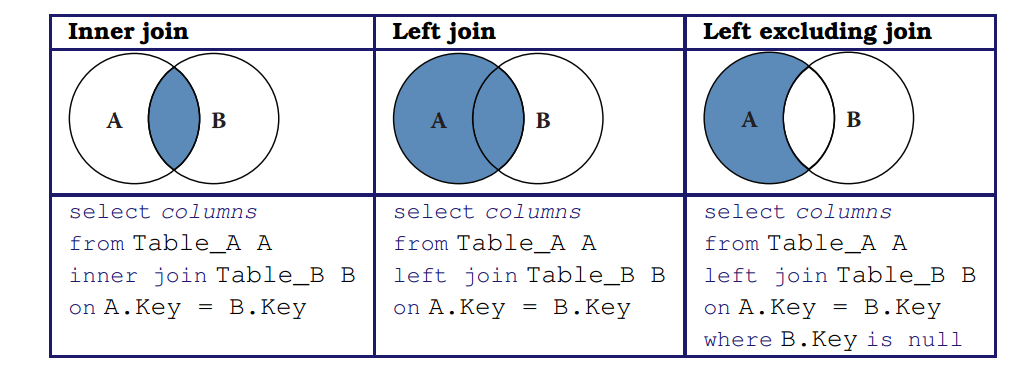
\includegraphics[width=0.7\linewidth]{ChapterDB/figures/fig-venn} 

}

\caption{Three types of *join* illustrated: the inner join, the left join, and left excluding join}\label{fig:fig-venn}
\end{figure}

\begin{center}\rule{0.5\linewidth}{\linethickness}\end{center}

\section{Which database to use?}\label{which-database-to-use}

The question of which DBMS to use for a social science project depends
on many factors. We introduced some relevant rules in Table
\ref{tab:table4-1}. We expand on those considerations here.

\subsection{Relational DBMSs}\label{relational-dbmss-1}

If your data are structured into rows and columns, then a relational
DBMS is almost certainly the right technology to use. Many open source,
commercial, and cloud-hosted relational DBMSs exist. Among the open
source DBMSs, MySQL and PostgreSQL (often simply called Postgres) are
particularly widely used. MySQL is the most popular. It is particularly
easy to install and use, but does not support all features of the SQL
standard. PostgreSQL is fully standard compliant and supports useful
features such as full text search and the PostGIS extensions mentioned
in the previous section. \textbf{We recommend you start with Postgres.}

Popular commercial relational DBMSs include Microsoft SQL Server,
Oracle, IBM DB2, Teradata, and Sybase. These systems are heavily used in
commercial settings. There are free community editions, and some large
science projects use enterprise features via licensing: for example, the
Sloan Digital Sky Survey uses Microsoft SQL Server (Szalay et al.
\protect\hyperlink{ref-szalay2002sdss}{2002}) and the CERN high-energy
physics lab uses Oracle (Girone
\protect\hyperlink{ref-girone2008cern}{2008}).

We also see increasing use being made of cloud-hosted relational DBMSs
such as Amazon Relational Database Service (RDS; this supports MySQL,
PostgreSQL, and various commercial DBMSs), Microsoft Azure, and Google
Cloud SQL. These systems obviate the need to install local software,
administer a DBMS, or acquire hardware to run and scale your database.
Particularly if your database is bigger than can fit on your
workstation, a cloud-hosted solution can be a good choice, both for
scalability but also for ease of configuration and management.

\subsection{NoSQL DBMSs}\label{nosql-dbmss}

Some social science problems have the scale that might motivate the use
of a NoSQL DBMS. Furthermore, while defining and enforcing a schema can
involve some effort, the benefits of so doing are considerable. Thus,
the use of a relational DBMS is usually to be recommended.

Nevertheless, as noted in Section \protect\hyperlink{sec:db:when}{DBMS:
When and why}, there are occasions when a NoSQL DBMS can be a highly
effective, such as when working with large quantities of unstructured
data. For example, researchers analyzing large collections of Twitter
messages frequently store the messages in a NoSQL document-oriented
database such as MongoDB. NoSQL databases are also often used to
organize large numbers of records from many different sources, as
illustrated in Figure \ref{fig:figdb-dbs}.

\section{Summary}\label{summary-2}

A key message of this book is that you should, whenever possible, use a
database. Database management systems are one of the great achievements
of information technology, permitting large amounts of data to be stored
and organized so as to allow rapid and reliable exploration and
analysis. They have become a central component of a great variety of
applications, from handling transactions in financial systems to serving
data published in websites. They are particularly well suited for
organizing social science data and for supporting analytics for data
exploration.

DBMSs provide an environment that greatly simplifies data management and
manipulation. They make many easy things trivial, and many hard things
easy. They automate many other error-prone, manual tasks associated with
query optimization. While they can by daunting to those unfamiliar with
their concepts and workings, they are in fact easy to use. A basic
understanding of databases and of when and how to use DBMSs is an
important element of the social data scientist's knowledge base.

\section{Resources}\label{resources-1}

The enormous popularity of DBMSs means that there are many good books to
be found. Classic textbooks such as those by Silberschatz et al.
(\protect\hyperlink{ref-silberschatz2010database}{2010}) and
Ramakrishnan and Gherke
(\protect\hyperlink{ref-ramakrishnan2000database}{2002}) provide a great
deal of technical detail. The DB Engines website collects information on
DBMSs.\footnote{\url{http://db-engines.com/en/}} There are also many
useful online tutorials, and of course StackExchange and other online
forums often have answers to your technical questions.

Turning to specific technologies, the \emph{SQL Cookbook} (Molinaro
\protect\hyperlink{ref-SQLCookbook}{2005}) provides a wonderful
introduction to SQL. We also recommend the SQL Cheatsheet\footnote{\url{http://www.sql-tutorial.net/SQL-Cheat-Sheet.pdf}}
and a useful visual depiction of different SQL join operators (Moffatt
\protect\hyperlink{ref-vizjoins}{1999}). Two good books on the PostGIS
geospatial extensions to the PostgreSQL database are the \emph{PostGIS
Cookbook} (Corti et al. \protect\hyperlink{ref-PostGISCookbook}{2014})
and \emph{PostGIS in Action} (Obe and Hsu
\protect\hyperlink{ref-PostGISInAction}{2015}). The online documentation
is also excellent.\footnote{\url{http://postgis.net/documentation/}} The
monograph \emph{NoSQL Databases} (Strauch
\protect\hyperlink{ref-NoSQLdatabases}{2009}) provides much useful
technical detail.

We did not consider in this chapter the native extensible Markup
Language (XML) and Resource Description Framework (RDF) triple stores,
as these are not typically used for data management. However, they do
play a fundamental role in metadata and knowledge management. See, for
example, Sesame (Broekstra, Kampman, and Van Harmelen
\protect\hyperlink{ref-broekstra2002sesame}{2002}).\footnote{\url{http://rdf4j.org}}

If you are interested in the state of database and data management
research, the relatively recent Beckman Report (Abadi et al.
\protect\hyperlink{ref-abadi2014beckman}{2014}) provides a useful
perspective.

The \emph{Databases} notebook of Chapter
\protect\hyperlink{chap:workbooks}{Workbooks} provides an introduction
to working with SQL.\footnote{See
  \url{https://workbooks.coleridgeinitiative.org}.}

\hypertarget{chap:parallel}{\chapter{Scaling up through Parallel and
Distributed Computing}\label{chap:parallel}}

\textbf{Huy Vo and Claudio Silva}

This chapter provides an overview of techniques that allow us to analyze
large amounts of data using distributed computing (multiple computers
concurrently). While the focus is on a widely used framework called
MapReduce and popular implementations such as Apache Hadoop and Spark,
the goal of the chapter is to provide a conceptual and practical
framework to deal with large amounts of data that may not fit in memory
or take too long to analyze on a single computer. It is important to
note that these frameworks do not result in analysis that is
better---they are useful because they allow us to process large amounts
of data faster and/or without getting access to a single massive
computer with lots of memory (RAM) and processing power (CPU).

\section{Introduction}\label{introduction-1}

As the amount of data available for social science research increases,
we have to determine how to perform our analysis quickly and
efficiently. One way to deal with large amounts of data that may not fit
in memory or take too long to analyze on a single computer is to
subsample the data or to simplify the analysis. Another approach is to
use all the data by making use of multiple computers concurrently to do
the analysis. The use of parallel computing to deal with large amounts
of data has been a common approach in physical sciences. Data analysts
have routinely been working on data sets much larger than a single
machine can handle for several decades, especially at the DOE National
Laboratories (Sethian et al. \protect\hyperlink{ref-bigdata_old1}{1991};
Crossno, Cline, and Jortner
\protect\hyperlink{ref-crossno1993heterogeneous}{1993}) where
high-performance computing has been a major technology trend. This is
also demonstrated by the history of research in distributed computing
and data management going back to the 1980s.

There are many ways to do distributed and parallel computing, ranging
from completely flexible (but more complex to use) approaches such as
Message Passing Interface (MPI) (Gropp, Lusk, and Skjellum
\protect\hyperlink{ref-mpi}{2014}) to more restrictive (but much easier
to use) approaches such as MapReduce. MPI allows you to do anything with
as much efficiency as your MPI skills allow you to code while MapReduce
allows a more restrictive set of analysis to be done (possibly less
efficiently) but is much easier to learn and implement.

This chapter focuses on one such framework, called MapReduce, to do
large-scale data analysis distributed across multiple computers. We
describe the MapReduce framework, work through an example of using it,
and highlight one implementation of the framework called Hadoop in
detail.\footnote{If you have examples from your own research using the
  methods we describe in this chapter, please submit a link to the paper
  (and/or code) here:
  \url{https://textbook.coleridgeinitiative.org/submitexamples}}

\begin{center}\rule{0.5\linewidth}{\linethickness}\end{center}

\textbf{Box: Parallel Computing Examples}

Al Aghbari et al. (\protect\hyperlink{ref-aghbari2019}{2019}) introduce
GeoSim, an algorithm used for clustering users in any social network
site into communities based on the semantic meaning of the nodes
interests as well as their relationships with each other. The
parallelised version of GeoSim utilizes the MapReduce model to run on
multiple machines simultaneously and get faster results.

Kolb et al. (\protect\hyperlink{ref-kolb2012}{2012}) developed a tool
DeDoop that uses Hadoop to do efficient record linkage (remember chapter
\protect\hyperlink{chap:link}{Record Linkage}?) and scale to large data
sets. Tasks such as record linkage where we can easily break down the
larger task into smaller chunks (such as comparing two records to see if
they belong to the same entity) that can be done in parallel are ideally
suited for MapReduce frameworks.

Ching et al. (\protect\hyperlink{ref-ching2012}{2012}) describe the data
infrastructure at Facebook with MapReduce at the core of Facebook's data
analytics engine. Over half a petabyte of new data arrives in the
warehouse every 24 hours, and ad-hoc queries, data pipelines, and custom
MapReduce jobs process this raw data around the clock to generate more
meaningful features and aggregations.

\begin{center}\rule{0.5\linewidth}{\linethickness}\end{center}

\section{MapReduce}\label{mapreduce}

The MapReduce framework was proposed by Jeffrey Dean and Sanjay Ghemawat
at Google in 2004 (Dean and Ghemawat
\protect\hyperlink{ref-MapReduce}{2004}). Its origins date back to
conceptually similar approaches first described in the early 1980s.
Using the MapReduce framework requires turning the analysis problem we
have into operations that the framework supports---these are map and
reduce. The ``map'' operation takes the input and splits up the task
into multiple (parallel) components, and the ``reduce'' operation
consolidates the results of the parallel ``mapped'' tasks and produces
the final output. In order to use the MapReduce framework, we need to
break up our tasks in to map and reduce operations and implement these
two operations.

\begin{center}\rule{0.5\linewidth}{\linethickness}\end{center}

\textbf{Example: Counting NSF awards}

To gain a better understanding of these MapReduce operations, let's take
a trivial task that may need to be done on billions of records, causing
scalability challenges. Imagine that we have a list of NSF principal
investigators, along with their email information and award IDs as
below. Our task is to count the number of awards for each institution.
For example, given the four records below, we will discover that the
Berkeley Geochronology Center has two awards, while New York University
and the University of Utah each have one.

\begin{verbatim}
AwardId,FirstName,LastName,EmailAddress
0958723,Roland,Mundil,rmundil@bgc.org
0958915,Randall,Irmis,irmis@umnh.utah.edu
1301647,Zaher,Hani,zh8@nyu.edu
1316375,David,Shuster,dshuster@bgc.org
\end{verbatim}

We observe that institutions can be distinguished by their email address
domain name. Thus, we adopt a strategy of first grouping all award IDs
by domain names, and then counting the number of distinct awards within
each group. In order to do this, we first set the function to scan input
lines and extract institution information and award IDs. Then, in the
function, we simply count unique IDs on the data, since everything is
already grouped by institution. Python pseudo-code is provided in
Listing \protect\hyperlink{list:parallel1}{MapReduce}.

\begin{Shaded}
\begin{Highlighting}[]
\CommentTok{# Input  : a list of text lines}
\CommentTok{# Output : a list of domain name and award ids}
\KeywordTok{def}\NormalTok{ MAP(lines):}
    \ControlFlowTok{for}\NormalTok{ line }\KeywordTok{in}\NormalTok{ lines:}
\NormalTok{        fields     }\OperatorTok{=}\NormalTok{ line.strip(}\StringTok{'}\CharTok{\textbackslash{}n}\StringTok{'}\NormalTok{).split(}\StringTok{','}\NormalTok{)}
\NormalTok{        awardId    }\OperatorTok{=}\NormalTok{ fields[}\DecValTok{0}\NormalTok{]}
\NormalTok{        domainName }\OperatorTok{=}\NormalTok{ fields[}\DecValTok{3}\NormalTok{].split(}\StringTok{'@'}\NormalTok{)[}\OperatorTok{-}\DecValTok{1}\NormalTok{].split(}\StringTok{'.'}\NormalTok{)[}\OperatorTok{-}\DecValTok{2}\NormalTok{:]}
        \ControlFlowTok{yield}\NormalTok{ (domainName, awardId)}

\CommentTok{# Input  : a list of domain name and award ids}
\CommentTok{# Output : a list of domain name and award count}
\KeywordTok{def}\NormalTok{ REDUCE(pairs):}
    \ControlFlowTok{for}\NormalTok{ (domainName, awardIds) }\KeywordTok{in}\NormalTok{ pairs:}
\NormalTok{        count }\OperatorTok{=} \BuiltInTok{len}\NormalTok{(}\BuiltInTok{set}\NormalTok{(awardIds))}
        \ControlFlowTok{yield}\NormalTok{ (domainName, count)}
\end{Highlighting}
\end{Shaded}

Listing: Python pseudo-code for the \texttt{map} and \texttt{reduce}
functions to count the number of awards per institution

In the map phase, the input will be transformed into tuples of
institutions and award ids:

\texttt{"0958723,Roland,Mundil,rmundil@bgc.org"} →
\texttt{("bgc.org",\ 0958723)}
\texttt{"0958915,Randall,Irmis,irmis@umnh.utah.edu"} →
\texttt{("utah.edu",\ 0958915)}
\texttt{"1301647,Zaher,Hani,zh8@nyu.edu"} →
\texttt{("nyu.edu",\ 1301647)}
\texttt{"1316375,David,Shuster,dshuster@bgc.org"} →
\texttt{("bgc.org",\ 1316375)}

Then the tuples will be grouped by institutions and be counted by the
function.

\texttt{("bgc.org",\ {[}0958723,1316375{]})} → \texttt{("bgc.org",\ 2)}
\texttt{("utah.edu",\ \textbackslash{}{[}0958915\textbackslash{}{]})} →
\texttt{("utah.edu",\ 1)}
\texttt{("nyu.edu",\ \textbackslash{}{[}1301647\textbackslash{}{]})} →
\texttt{("nyu.edu",\ 1)}

As we have seen so far, the MapReduce programming model is quite simple
and straightforward, yet it supports a simple parallelization model. In
fact, it has been said to be \emph{too} simple and criticized as ``a
major step backwards'' (DeWitt and Stonebraker
\protect\hyperlink{ref-MapReduceBad}{2008}) for large-scale,
data-intensive applications. It is hard to argue that MapReduce is
offering something truly innovative when MPI has been offering similar
scatter and reduce operations since 1995, and Python has had high-order
functions (\texttt{map}, \texttt{reduce}, \texttt{filter}, and
\texttt{lambda}) since its 2.2 release in 1994. However, the biggest
strength of MapReduce is its simplicity. Its simple programming model
has brought many non-expert users to analyzing large amounts of data.
Its simple architecture has also inspired many developers to develop
advanced capabilities, such as support for distributed computing, data
partitioning, and streaming processing. A downside of this diversity of
interest is that available features and capabilities can vary
considerably, depending on the specific implementation of MapReduce that
is being used.

As mentioned above, MapReduce is a programming model. In order to
implement an analysis in MapReduce, we need to select an implementation
of MapReduce. Two most commonly used implementations of the MapReduce
model are Hadoop and Spark, that we describe in more detail below.

\section{Apache Hadoop MapReduce}\label{apache-hadoop-mapreduce}

Apache Hadoop (or Hadoop)\footnote{The term \emph{Hadoop} refers to the
  creator's son's toy elephant.} was originally designed to run in
environments with thousands of machines. Supporting such a large
computing environment puts several constraints on the system; for
instance, with so many machines, the system had to assume computing
nodes would fail. Hadoop is an enhanced MapReduce implementation with
the support for fault tolerance, distributed storage, and data
parallelism through two added key design features: (1) a distributed
file system called the Hadoop Distributed File System (HDFS); and (2) a
data distribution strategy that allows computation to be moved to the
data during execution.

\subsection{The Hadoop Distributed File
System}\label{the-hadoop-distributed-file-system}

The Hadoop Distributed File System (Apache Hadoop, n.d.) is a
distributed file system that stores data across all the nodes (machines)
of a Hadoop cluster.\footnote{\url{https://hadoop.apache.org/docs/stable/}}
HDFS splits large data files into smaller blocks (chunks of data) which
are managed by different nodes in a cluster. Each block is also
replicated across several nodes as an attempt to ensure that a full copy
of the data is still available even in the case of computing node
failures. The block size as well as the number of replications per block
are fully customized by users when they create files on HDFS. By
default, the block size is set to 64 MB with a replication factor of 3,
meaning that the system may encounter at least two concurrent node
failures without losing any data. HDFS also actively monitors failures
and re-replicates blocks on failed nodes to make sure that the number of
replications for each block always stays at the user-defined settings.
Thus, if a node fails, and only two copies of some data exist, the
system will quickly copy those data to a working node, thus raising the
number of copies to three again. This dynamic replication is the primary
mechanism for fault tolerance in Hadoop.

Note that data blocks are replicated and distributed across several
machines. This could create a problem for users, because if they had to
manage the data manually, they might, for example, have to access more
than one machine to fetch a large data file. Fortunately, Hadoop
provides infrastructure for managing this complexity seamlessly,
including command line programs as well as an API that users can employ
to interact with HDFS as if it were a local file system. For example,
one can run simple Linux commands such as ls and mkdir to list and
create a directory on HDFS, or even use to inspect file contents the
same way as one would do in a Linux file system. The following code
shows some examples of interacting with HDFS.

\begin{Shaded}
\begin{Highlighting}[]
\CommentTok{# Creating a folder}
\NormalTok{hadoop dfs }\OperatorTok{-}\NormalTok{mkdir }\OperatorTok{/}\NormalTok{hadoopiseasy}

\CommentTok{# Upload a CSV file from our local machine to HDFS}
\NormalTok{hadoop dfs }\OperatorTok{-}\NormalTok{put importantdata.csv }\OperatorTok{/}\NormalTok{hadoopiseasy}

\CommentTok{# Listing all files under hadoopiseasy folder}
\NormalTok{hadoop dfs }\OperatorTok{-}\NormalTok{ls }\OperatorTok{/}\NormalTok{hadoopiseasy}

\CommentTok{# Download a file to our local machine}
\NormalTok{hadoop dfs }\OperatorTok{-}\NormalTok{get }\OperatorTok{/}\NormalTok{hadoopiseasy}\OperatorTok{/}\NormalTok{importantdata.csv}
\end{Highlighting}
\end{Shaded}

\subsection{Hadoop Setup: Bringing compute to the
data}\label{hadoop-setup-bringing-compute-to-the-data}

There are two parts of the computing environment when using Hadoop: 1. a
\emph{compute cluster} with substantial computing power (e.g., thousands
of computing cores) 2. a \emph{storage cluster} with lots of disk space,
capable of storing and serving data quickly to the compute cluster.

These two clusters have quite different hardware specifications: the
first is optimized for CPU performance and the second for storage. The
two systems are typically configured as separate physical hardware.

\begin{center}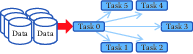
\includegraphics[width=0.7\linewidth]{ChapterParallel/figures/data2compute} \end{center}

\begin{figure}

{\centering 
\includegraphics[width=0.7\linewidth]{ChapterParallel/figures/compute2data} 

}

\caption{Top: The traditional parallel computing model where data are brought to the computing nodes. Bottom: Hadoop’s parallel computing model: bringing compute to the data [@HadoopParallelModel]}\label{fig:fig5-1a}
\end{figure}

Running compute jobs on such hardware often goes like this. When a user
requests to run an intensive task on a particular data set, the system
will first reserve a set of computing nodes. Then the data are
partitioned and copied from the storage server into these computing
nodes before the task is executed. This process is illustrated in Figure
\ref{fig:fig5-1a} (top). This computing model will be referred to as
\emph{bringing data to computation}. In this model, if a data set is
being analyzed in multiple iterations, it is very likely that the data
will be copied multiple times from the storage cluster to the compute
nodes without reusability. This is because the compute node scheduler
normally does not have or keep knowledge of where data have previously
been held. The need to copy data multiple times tends to make such a
computation model inefficient, and I/O becomes the bottleneck when all
tasks constantly pull data from the storage cluster (the red arrow).
This in turn leads to poor scalability; adding more nodes to the
computing cluster would not increase its performance.

To solve this problem, Hadoop implements a \emph{bring compute to the
data} strategy that combines both computing and storage at each node of
the cluster. In this setup, each node offers both computing power and
storage capacity. As shown in Figure \ref{fig:fig5-1a} (bottom), when
users submit a task to be run on a data set, the scheduler will first
look for nodes that contain the data, and if the nodes are available, it
will schedule the task to run directly on those nodes. If a node is busy
with another task, data will still be copied to available nodes, but the
scheduler will maintain records of the copy for subsequent use of the
data. In addition, data copying can be minimized by increasing the data
duplication in the cluster, which also increases the potential for
parallelism, since the scheduler has more choices to allocate computing
without copying. Since both the compute and data storage are closely
coupled for this model, it is best suited for data-intensive
applications.

Given that Hadoop was designed for batch data processing at scale, this
model fits the system nicely, especially with the support of HDFS.
However, in an environment where tasks are more compute intensive, a
traditional high-performance computing environment is probably best
since it tends to spend more resources on CPU cores. It should be clear
now that the Hadoop model has hardware implications, and computer
architects have optimized systems for data-intensive computing.

\subsection{Hardware provisioning}\label{hardware-provisioning}

Hadoop requires a distributed cluster of machines to operate
efficiently. (It can be set up to run entirely on a single computer, but
this should only be done for technology demonstration purposes.) This is
mostly because the MapReduce performance heavily depends on the total
I/O throughput (i.e., disk read and write) of the entire system. Having
a distributed cluster, where each machine has its own set of hard
drives, is one of the most efficient ways to maximize this throughput.

A typical Hadoop cluster consists of two types of machine: masters and
workers. Master machines are those exclusively reserved for running
services that are critical to the framework operations. Some examples
are the NameNode and the JobTracker services, which are tasked to manage
how data and tasks are distributed among the machines, respectively. The
worker machines are reserved for data storage and for running actual
computation tasks (i.e., map and reduce). It is normal to have worker
machines that can be included or removed from an operational cluster on
demand. This ability to vary the number of worker nodes makes the
overall system more tolerant of failure. However, master machines are
usually required to be running uninterrupted.

Provisioning and configuring the hardware for Hadoop, like any other
parallel computing, are some of the most important and complex tasks in
setting up a cluster, and they often require a lot of experience and
careful consideration. Major big data vendors provide guidelines and
tools to facilitate the process (Apache Software Foundation, n.d.;
Cloudera, n.d.; Baldeschwieler
\protect\hyperlink{ref-Provisioning}{2011}). most decisions will be
based on the types of analysis to be run on the cluster, for which only
you, as the user, can provide the best input.

\subsection{Programming in Hadoop}\label{programming-in-hadoop}

Now that we are equipped with the knowledge that Hadoop is a MapReduce
implementation that runs on HDFS and a bring-compute-to-the-data model,
we can go over the design of a Hadoop MapReduce job. A MapReduce job is
still composed of three phases: map, shuffle, and reduce. However,
Hadoop divides the map and reduce phases into smaller tasks.

Each map phase in Hadoop is divided into five tasks: \textbf{input
format}, \textbf{record reader}, \textbf{mapper}, \textbf{combiner}, and
\textbf{partitioner}. An \emph{input format} task is in charge of
talking to the input data presumably sitting on HDFS, and splitting it
into partitions (e.g., by breaking lines at line breaks). Then a
\emph{record reader} task is responsible for translating the split data
into the key--value pair records so that they can be processed by the
mapper. By default, Hadoop parses files into key--value pairs of line
numbers and line contents. However, both input formats and record
readers are fully customizable and can be programmed to read custom data
including binary files. It is important to note that input formats and
record readers only provide data partitioning; they do not move data
around computing nodes.

After the records are generated, mappers are spawned---typically on
nodes containing the blocks---to run through these records and output
zero or more new key--value pairs. A mapper in Hadoop is equivalent to
the \texttt{map} function of the MapReduce model that we discussed
earlier. The selection of the key to be output from the mapper will
heavily depend on the data processing pipeline and could greatly affect
the performance of the framework. Mappers are executed concurrently in
Hadoop as long as resources permit.

A combiner task in Hadoop is similar to a function in the MapReduce
framework, but it only works locally at each node: it takes output from
mappers executed on the same node and produces aggregated values.
Combiners are optional but can be used to greatly reduce the amount of
data exchange in the shuffle phase; thus, users are encouraged to
implement this whenever possible. A common practice is when a
\texttt{reduce} function is both commutative and associative, and has
the same input and output format, one can just use the \texttt{reduce}
function as the combiner. Nevertheless, combiners are not guaranteed to
be executed by Hadoop, so this should only be treated as a hint. Its
execution must not affect the correctness of the program.

A partitioner task is the last process taking place in the map phase on
each mapper node, where it hashes the key of each key--value pair output
from the mappers or the combiners into bins. By default, the partitioner
uses object hash codes and modulus operations to direct a designated
reducer to pull data from a map node. Though it is possible to customize
the partitioner, it is only advisable to do so when one fully
understands the intermediate data distribution as well as the
specifications of the cluster. In general, it is better to leave this
job to Hadoop.

Each reduce phase in Hadoop is divided into three tasks:
\textbf{reducer}, \textbf{output format}, and \textbf{record writer}.
The \texttt{reducer} task is equivalent to the \texttt{reduce} function
of the MapReduce model. It basically groups the data produced by the
mappers by keys and runs a \texttt{reduce} function on each list of
grouping values. It outputs zero or more key--value pairs for the output
format task, which then translates them into a writable format for the
record writer task to serialize on HDFS. By default, Hadoop will
separate the key and value with a tab and write separate records on
separate lines. However, this behavior is fully customizable. Similarly,
the map phase reducers are also executed concurrently in Hadoop.

\begin{figure}

{\centering 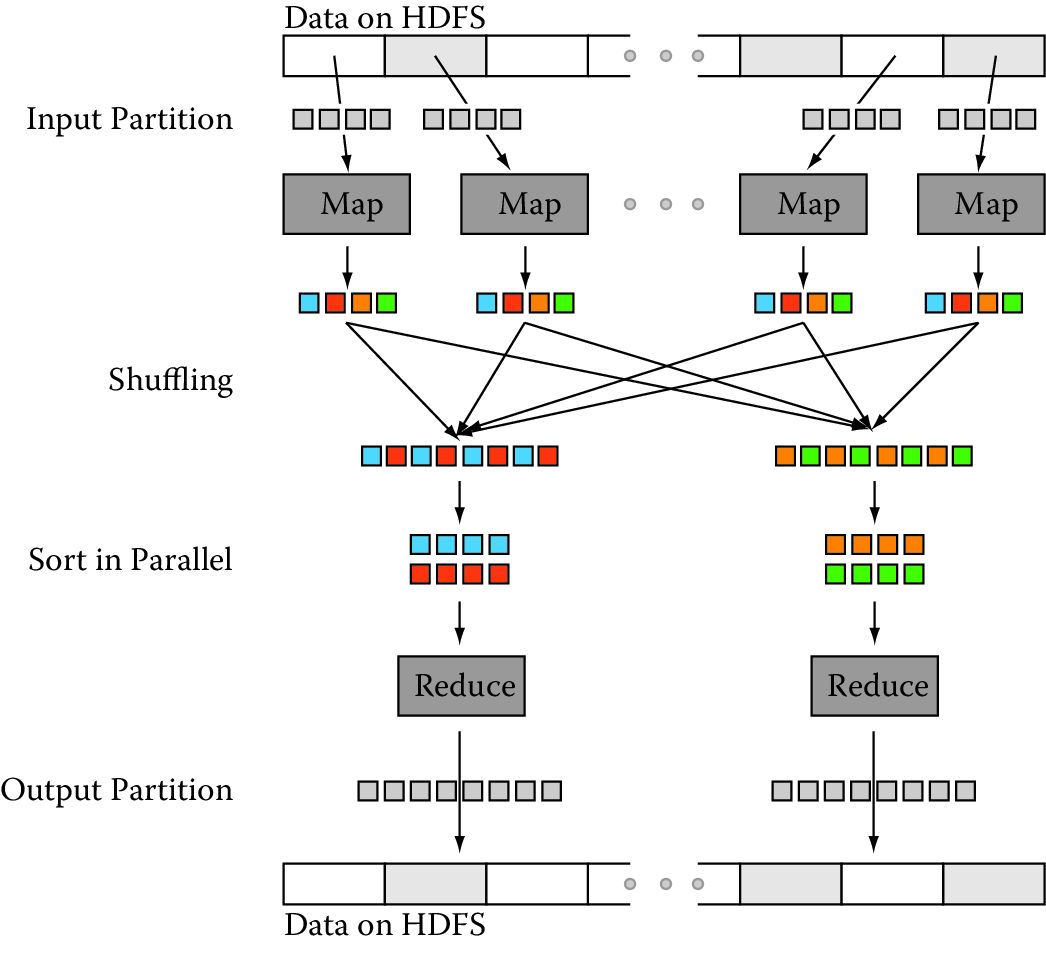
\includegraphics[width=0.7\linewidth]{ChapterParallel/figures/hadoop} 

}

\caption{Data transfer and communication of a MapReduce job in Hadoop. Data blocks are assigned to several maps, which emit key--value pairs that are shuffled and sorted in parallel. The reduce step emits one or more pairs, with results stored on the HDFS}\label{fig:hadoop}
\end{figure}

\subsection{Programming language
support}\label{programming-language-support}

Hadoop is written entirely in Java, thus it is best supporting
applications written in Java. However, Hadoop also provides a
\emph{streaming API} that allows arbitrary code to be run inside the
Hadoop MapReduce framework through the use of UNIX pipes. This means
that we can supply a mapper program written in Python or C++ to Hadoop
as long as that program reads from the standard input and writes to the
standard output. The same mechanism also applies for the combiner and
reducer. For example, we can develop from the Python pseudo-code in
Listing \protect\hyperlink{list:parallel1}{MapReduce} to a complete
Hadoop streaming mapper (Listing
\protect\hyperlink{list:parallel2}{Mapper}) and reducer (Listing
\protect\hyperlink{list:parallel3}{Reducer}).

\begin{Shaded}
\begin{Highlighting}[]
\CommentTok{#!/usr/bin/env python}
\ImportTok{import}\NormalTok{ sys}

\KeywordTok{def}\NormalTok{ parseInput():}
    \ControlFlowTok{for}\NormalTok{ line }\KeywordTok{in}\NormalTok{ sys.stdin:}
        \ControlFlowTok{yield}\NormalTok{ line}

\ControlFlowTok{if} \VariableTok{__name__}\OperatorTok{==}\StringTok{'__main__'}\NormalTok{:}
    \ControlFlowTok{for}\NormalTok{ line }\KeywordTok{in}\NormalTok{ parseInput():}
\NormalTok{        fields     }\OperatorTok{=}\NormalTok{ line.strip(}\StringTok{'}\CharTok{\textbackslash{}n}\StringTok{'}\NormalTok{).split(}\StringTok{','}\NormalTok{)}
\NormalTok{        awardId    }\OperatorTok{=}\NormalTok{ fields[}\DecValTok{0}\NormalTok{]}
\NormalTok{        domainName }\OperatorTok{=}\NormalTok{ fields[}\DecValTok{3}\NormalTok{].split(}\StringTok{'@'}\NormalTok{)[}\OperatorTok{-}\DecValTok{1}\NormalTok{].split(}\StringTok{'.'}\NormalTok{)[}\OperatorTok{-}\DecValTok{2}\NormalTok{:]}
        \BuiltInTok{print}\NormalTok{(}\StringTok{'}\SpecialCharTok{%s}\CharTok{\textbackslash{}t}\SpecialCharTok\NormalTok{ (domainName,awardId))}
\end{Highlighting}
\end{Shaded}

Listing: A Hadoop streaming mapper in Python

\begin{Shaded}
\begin{Highlighting}[]
\CommentTok{#!/usr/bin/env python}
\ImportTok{import}\NormalTok{ sys}

\KeywordTok{def}\NormalTok{ parseInput():}
    \ControlFlowTok{for}\NormalTok{ line }\KeywordTok{in}\NormalTok{ sys.stdin:}
        \ControlFlowTok{yield}\NormalTok{ line}

\ControlFlowTok{if} \VariableTok{__name__}\OperatorTok{==}\StringTok{'__main__'}\NormalTok{:}
    \ControlFlowTok{for}\NormalTok{ line }\KeywordTok{in}\NormalTok{ parseInput():}
\NormalTok{        (domainName, awardIds) }\OperatorTok{=}\NormalTok{ line.split(}\StringTok{'}\CharTok{\textbackslash{}t}\StringTok{'}\NormalTok{)}
\NormalTok{        count }\OperatorTok{=} \BuiltInTok{len}\NormalTok{(}\BuiltInTok{set}\NormalTok{(awardIds))}
        \BuiltInTok{print}\NormalTok{(}\StringTok{'}\SpecialCharTok{%s}\CharTok{\textbackslash{}t}\SpecialCharTok\NormalTok{ (domainName, count))}
\end{Highlighting}
\end{Shaded}

Listing: A Hadoop streaming reducer in Python

It should be noted that in Hadoop streaming, intermediate key--value
pairs (the data flowing between mappers and reducers) must be in
tab-delimited format, thus we replace the original \texttt{yield}
command with a \texttt{print} formatted with tabs. Though the input
format and record reader are still customizable in Hadoop streaming,
they must be supplied as Java classes. This is one of the biggest
limitations of Hadoop for Python developers. They not only have to split
their code into separate mapper and reducer programs, but also need to
learn Java if they want to work with nontextual data.

\subsection{Benefits and Limitations of
Hadoop}\label{benefits-and-limitations-of-hadoop}

\begin{itemize}
\item
  \textbf{Fault Tolerance}: By default, HDFS uses checksums to enforce
  data integrity on its file system and data replication for recovery of
  potential data losses. Taking advantage of this, Hadoop also maintains
  fault tolerance of MapReduce jobs by storing data at every step of a
  MapReduce job to HDFS, including intermediate data from the combiner.
  Then the system checks whether a task fails by either looking at its
  heartbeats (data activities) or whether it has been taking too long.
  If a task is deemed to have failed, Hadoop will kill it and run it
  again on a different node. The time limit for the heartbeats and task
  running duration may also be customized for each job. Though the
  mechanism is simple, it works well on thousands of machines. It is
  indeed highly robust because of the simplicity of the model.
\item
  \textbf{Performance}: Hadoop has proven to be a scalable
  implementation that can run on thousands of cores. However, it is also
  known for having a relatively high job setup overhead and suboptimal
  running time. An empty task in Hadoop (i.e., with no mapper or
  reducer) can take roughly 30 seconds to complete even on a modern
  cluster. This overhead makes it unsuitable for real-time data or
  interactive jobs. The problem comes mostly from the fact that Hadoop
  monitoring processes only live within a job, thus it needs to start
  and stop these processes each time a job is submitted, which in turns
  results in this major overhead. Moreover, the brute force approach of
  maintaining fault tolerance by storing everything on HDFS is
  expensive, especially for large data sets.
\item
  \textbf{Hadoop streaming support for non-Java applications}: As
  mentioned previously, non-Java applications may only be integrated
  with Hadoop through the Hadoop streaming API. However, this API is far
  from optimal. First, input formats and record readers can only be
  written in Java, making it impossible to write advanced MapReduce jobs
  entirely in a different language. Second, Hadoop streaming only
  communicates with Hadoop through Unix pipes, and there is no support
  for data passing within the application using native data structure
  (e.g., it is necessary to convert Python tuples into strings in the
  mappers and convert them back into tuples again in reducers).
\item
  \textbf{Real-time applications}: With the current setup, Hadoop only
  supports batch data processing jobs. This is by design, so it is not
  exactly a limitation of Hadoop. However, given that more and more
  applications are dealing with real-time massive data sets, the
  community using MapReduce for real-time processing is constantly
  growing. Not having support for streaming or real-time data is clearly
  a disadvantage of Hadoop over other implementations.
\item
  \textbf{Limited data transformation operations}: This is more of a
  limitation of MapReduce than Hadoop per se. MapReduce only supports
  two operations, map and reduce, and while these operations are
  sufficient to describe a variety of data processing pipelines, there
  are classes of applications that MapReduce is not suitable for. Beyond
  that, developers often find themselves rewriting simple data
  operations such as data set joins, finding a min or max, and so on.
  Sometime, these tasks require more than one map-and-reduce operation,
  resulting in multiple MapReduce jobs. This is both cumbersome and
  inefficient. There are tools to automate this process for Hadoop;
  however, they are only a layer above, and it is not easy to integrate
  with existing customized Hadoop applications.
\end{itemize}

\section{Other MapReduce
Implementations}\label{other-mapreduce-implementations}

In addition to Apache Hadoop, other notable MapReduce implementations
include MongoDB, GreenplumDB, Disco, Riak, and Spark. MongoDB, Riak, and
Greenplum DB are all database systems\footnote{See Chapter
  \protect\hyperlink{chap:db}{Databases}.} and thus their MapReduce
implementations focus more on the interoperability of MapReduce and the
core components such as MongoDB's aggregation framework, and leave it up
to users to customize the MapReduce functionalities for broader tasks.
Some of these systems, such as Riak, only parallelize the map phase, and
run the reduce phase on the local machine that request the tasks. The
main advantage of the three implementations is the ease with which they
connect to specific data stores. However, their support for general data
processing pipelines is not as extensive as that of Hadoop.

Disco, similar to Hadoop, is designed to support MapReduce in a
distributed computing environment, but it is written in Erlang with a
Python interface. Thus, for Python developers, Disco might be a better
fit. However, it has significantly fewer supporting applications, such
as access control and workflow integration, as well as a smaller
developing community. This is why the top three big data platforms,
Cloudera, Hortonworks, and MapR, still build primarily on Hadoop.

\section{Apache Spark}\label{apache-spark}

Apache Spark is another implementation that aims to support beyond
MapReduce. The framework is centered around the concept of resilient
distributed data sets and data transformations that can operate on these
objects. An innovation in Spark is that the fault tolerance of resilient
distributed data sets can be maintained without flushing data onto
disks, thus significantly improving the system performance (with a claim
of being 100 times faster than Hadoop). Instead, the fault-recovery
process is done by replaying a log of data transformations on
check-point data. Though this process could take longer than reading
data straight from HDFS, it does not occur often and is a fair tradeoff
between processing performance and recovery performance.

Beyond map and reduce, Spark also supports various other transformations
(Hadoop, n.d.), including filter, data join, and aggregation. Streaming
computation can also be done in Spark by asking Spark to reserve
resources on a cluster to constantly stream data to/from the cluster.
However, this streaming method might be resource intensive (still
consuming resources when there is no data coming). Additionally, Spark
plays well with the Hadoop ecosystem, particularly with the distributed
file system (HDFS) and resource manager (YARN), making it possible to be
built on top of current Hadoop applications.

Another advantage of Spark is that it supports Python natively; thus,
developers can run Spark in a fraction of the time required for Hadoop.
Listing \protect\hyperlink{list:parallel4}{Spark} provides the full code
for the previous example written entirely in Spark. It should be noted
that Spark's concept of the \texttt{reduceByKey} operator is not the
same as Hadoop's, as it is designed to aggregate all elements of a data
set into a single element. The closest simulation of Hadoop's MapReduce
pattern is a combination of \texttt{mapPartitions}, \texttt{groupByKey}
and \texttt{mapPartitions}, as shown in the next example.

\begin{Shaded}
\begin{Highlighting}[]
\ImportTok{import}\NormalTok{ sys}
\ImportTok{from}\NormalTok{ pyspark }\ImportTok{import}\NormalTok{ SparkContext}
\KeywordTok{def}\NormalTok{ mapper(lines):}
    \ControlFlowTok{for}\NormalTok{ line }\KeywordTok{in}\NormalTok{ lines:}
\NormalTok{        fields     }\OperatorTok{=}\NormalTok{ line.strip(}\StringTok{'}\CharTok{\textbackslash{}n}\StringTok{'}\NormalTok{).split(}\StringTok{','}\NormalTok{)}
\NormalTok{        awardId    }\OperatorTok{=}\NormalTok{ fields[}\DecValTok{0}\NormalTok{]}
\NormalTok{        domainName }\OperatorTok{=}\NormalTok{ fields[}\DecValTok{3}\NormalTok{].split(}\StringTok{'@'}\NormalTok{)[}\OperatorTok{-}\DecValTok{1}\NormalTok{].split(}\StringTok{'.'}\NormalTok{)[}\OperatorTok{-}\DecValTok{2}\NormalTok{:]}
        \ControlFlowTok{yield}\NormalTok{ (domainName, awardId)}

\KeywordTok{def}\NormalTok{ reducer(pairs):}
    \ControlFlowTok{for}\NormalTok{ (domainName, awardIds) }\KeywordTok{in}\NormalTok{ pairs:}
\NormalTok{        count }\OperatorTok{=} \BuiltInTok{len}\NormalTok{(}\BuiltInTok{set}\NormalTok{(awardIds))}
        \ControlFlowTok{yield}\NormalTok{ (domainName, count)}

\ControlFlowTok{if} \VariableTok{__name__}\OperatorTok{==}\StringTok{'__main__'}\NormalTok{:}
\NormalTok{    hdfsInputPath  }\OperatorTok{=}\NormalTok{ sys.argv[}\DecValTok{1}\NormalTok{]}
\NormalTok{    hdfsOutputFile }\OperatorTok{=}\NormalTok{  sys.argv[}\DecValTok{2}\NormalTok{]}
\NormalTok{    sc }\OperatorTok{=}\NormalTok{ SparkContext(appName}\OperatorTok{=}\StringTok{"Counting Awards"}\NormalTok{)}
\NormalTok{    output }\OperatorTok{=}\NormalTok{ sc.textFile(hdfsInputPath) }\OperatorTok{\textbackslash{}}
\NormalTok{        .mapPartitions(mapper) }\OperatorTok{\textbackslash{}}
\NormalTok{        .groupByKey() }\OperatorTok{\textbackslash{}}
\NormalTok{        .mapPartitions(reducer)}

\NormalTok{    output.saveAsTextFile(hdfsInputPath)}
\end{Highlighting}
\end{Shaded}

Listing: Python code for a Spark program that counts the number of
awards per institution using MapReduce

\begin{center}\rule{0.5\linewidth}{\linethickness}\end{center}

\textbf{Example: Analyzing home mortgage disclosure application data}

We use a financial services analysis problem to illustrate the use of
Apache Spark.

Mortgage origination data provided by the Consumer Protection Financial
Bureau provide insightful details of the financial health of the real
estate market. The data\footnote{\url{http://www.consumerfinance.gov/hmda/learn-more}},
which are a product of the Home Mortgage Disclosure Act (HMDA),
highlight key attributes that function as strong indicators of health
and lending patterns.

Lending institutions, as defined by section 1813 in Title 12 of the
HMDA, decide on whether to originate or deny mortgage applications based
on credit risk. In order to determine this credit risk, lenders must
evaluate certain features relative to the applicant, the underlying
property, and the location. We want to determine whether census tract
clusters could be created based on mortgage application data and whether
lending institutions' perception of risk is held constant across the
entire USA.

For the first step of this process, we study the debt--income ratio for
loans originating in different census tracts. This could be achieved
simply by computing the debt--income ratio for each loan application and
aggregating them for each year by census tract number. A challenge,
however, is that the data set provided by HMDA is quite extensive. In
total, HMDA data contain approximately 130 million loan applications
between 2007 and 2013. As each record contains 47 attributes, varying in
types from continuous variables such as loan amounts and applicant
income to categorical variables such as applicant gender, race, loan
type, and owner occupancy, the entire data set results in about 86 GB of
information. Parsing the data alone could take up to hours on a single
machine if using a naïve approach that scans through the data
sequentially. Tables \ref{tab:table5-1} and \ref{tab:table5-2} highlight
the breakdown in size per year and data fields of interest.

\begin{longtable}[]{@{}ccc@{}}
\caption{\label{tab:table5-1} Home Mortgage Disclosure Act data
size}\tabularnewline
\toprule
\textbf{Year} & \textbf{Records} & \textbf{File Size
(Gigabytes)}\tabularnewline
\midrule
\endfirsthead
\toprule
\textbf{Year} & \textbf{Records} & \textbf{File Size
(Gigabytes)}\tabularnewline
\midrule
\endhead
2007 & 26,605,696 & 18\tabularnewline
2008 & 17,391,571 & 12\tabularnewline
2009 & 19,493,492 & 13\tabularnewline
2010 & 16,348,558 & 11\tabularnewline
2011 & 14,873,416 & 9.4\tabularnewline
2012 & 18,691,552 & 12\tabularnewline
2013 & 17,016,160 & 11\tabularnewline
\textbf{Total} & \textbf{130,420,445} & \textbf{86.4}\tabularnewline
\bottomrule
\end{longtable}

\begin{longtable}[]{@{}llc@{}}
\caption{\label{tab:table5-2} Home Mortgage Disclosure Act data
size}\tabularnewline
\toprule
\textbf{Index} & \textbf{Attribute} & \textbf{Type}\tabularnewline
\midrule
\endfirsthead
\toprule
\textbf{Index} & \textbf{Attribute} & \textbf{Type}\tabularnewline
\midrule
\endhead
0 & Year & Integer\tabularnewline
1 & State & String\tabularnewline
2 & County & String\tabularnewline
3 & Census Tract & String\tabularnewline
4 & Loan Amount & Float\tabularnewline
5 & Applicant Income & Float\tabularnewline
6 & Loan Originated & Boolean\tabularnewline
\ldots{} & \ldots{} & \ldots{}\tabularnewline
\bottomrule
\end{longtable}

Observing the transactional nature of the data, where the aggregation
process could be distributed and merged across multiple partitions of
the data, we could complete this task in much less time by using Spark.
Using a cluster consisting of 1,200 cores, the Spark program in Listing
\protect\hyperlink{list:parallel5}{Census} took under a minute to
complete. The substantial performance gain comes not so much from the
large number of processors available, but mostly from the large I/O
bandwidth available on the cluster thanks to the 200 distributed hard
disks and fast network interconnects.

\begin{Shaded}
\begin{Highlighting}[]
\ImportTok{import}\NormalTok{ ast}
\ImportTok{import}\NormalTok{ sys}
\ImportTok{from}\NormalTok{ pyspark }\ImportTok{import}\NormalTok{ SparkContext}

\KeywordTok{def}\NormalTok{ mapper(lines):}
    \ControlFlowTok{for}\NormalTok{ line }\KeywordTok{in}\NormalTok{ lines:}
\NormalTok{        fields }\OperatorTok{=}\NormalTok{ ast.literal_eval(}\StringTok{'(}\SpecialCharTok\NormalTok{ line)}
\NormalTok{        (year, state, county, tract) }\OperatorTok{=}\NormalTok{ fields[:}\DecValTok{4}\NormalTok{]}
\NormalTok{        (amount, income, originated) }\OperatorTok{=}\NormalTok{ fields[}\DecValTok{4}\NormalTok{:]}

\NormalTok{        key }\OperatorTok{=}\NormalTok{ (year, state, county, tract)}
\NormalTok{        value }\OperatorTok{=}\NormalTok{ (amount, income)}

        \CommentTok{# Only count originated loans}
        \ControlFlowTok{if}\NormalTok{ originated:}
            \ControlFlowTok{yield}\NormalTok{ (key, value)}

\KeywordTok{def}\NormalTok{ sumDebtIncome(debtIncome1, debtIncome2):}
    \ControlFlowTok{return}\NormalTok{ (debtIncome1[}\DecValTok{0}\NormalTok{] }\OperatorTok{+}\NormalTok{ debtIncome2[}\DecValTok{0}\NormalTok{], debtIncome1[}\DecValTok{1}\NormalTok{] }\OperatorTok{+}\NormalTok{ debtIncome2[}\DecValTok{1}\NormalTok{])}

\ControlFlowTok{if} \VariableTok{__name__}\OperatorTok{==}\StringTok{'__main__'}\NormalTok{:}
\NormalTok{    hdfsInputPath  }\OperatorTok{=}\NormalTok{ sys.argv[}\DecValTok{1}\NormalTok{]}
\NormalTok{    hdfsOutputFile }\OperatorTok{=}\NormalTok{  sys.argv[}\DecValTok{2}\NormalTok{]}
\NormalTok{    sc }\OperatorTok{=}\NormalTok{ SparkContext(appName}\OperatorTok{=}\StringTok{"Debt-Income Ratio"}\NormalTok{)}
\NormalTok{    sumValues }\OperatorTok{=}\NormalTok{ sc.textFile(hdfsInputPath) }\OperatorTok{\textbackslash{}}
\NormalTok{        .mapPartitions(mapper) }\OperatorTok{\textbackslash{}}
\NormalTok{        .reduceByKey(sumDebtIncome)}

    \CommentTok{# Actually compute the aggregated debt income}
\NormalTok{    output }\OperatorTok{=}\NormalTok{ sumValues.mapValues(}\KeywordTok{lambda}\NormalTok{ debtIncome: debtIncome[}\DecValTok{0}\NormalTok{]}\OperatorTok{/}\NormalTok{debtIncome[}\DecValTok{1}\NormalTok{])}

\NormalTok{    output.saveAsTextFile(hdfsInputPath)}
\end{Highlighting}
\end{Shaded}

Listing: Python code for a Spark program to aggregate the debt--income
ratio for loans originated in different census tracts

\begin{center}\rule{0.5\linewidth}{\linethickness}\end{center}

\section{Summary}\label{summary-3}

Analyzing large amounts of data means that it is necessary to both store
very large collections of data and perform aggregate computations on
those data. This chapter describes an important data storage approach
(the Hadoop Distributed File System) and a way of processing large-scale
data sets (the MapReduce model, as implemented in both Hadoop and
Spark). This model enables not only large-scale data analysis but also
provides easy to use implementations for more flexibility for social
scientists to work with large amounts of data. This increases the
analytic throughput as well as the time to insight, speeding up the
decision-making process and thus increasing impact.

\section{Resources}\label{resources-2}

There are a wealth of online resources describing both Hadoop and Spark.
See, for example, the tutorials on the Apache Hadoop\footnote{\url{http://hadoop.apache.org/}}
and Spark\footnote{\url{https://spark.apache.org/}} websites. Albanese
describes how to use Hadoop for social science (Albanese
\protect\hyperlink{ref-socialhadoop}{2010}), and Lin and Dyer discuss
the use of MapReduce for text analysis (Lin and Dyer
\protect\hyperlink{ref-lin2010data}{2010}).

\hypertarget{chap:viz}{\chapter{Information
Visualization}\label{chap:viz}}

\textbf{M. Adil Yalcin and Catherine Plaisant}

This chapter will show you how to use visualization to explore data as
well as to communicate results so that data can be turned into
interpretable, actionable information. There are many ways of presenting
statistical information that convey content in a rigorous manner. The
goal of this chapter is to present an introductory overview of effective
visualization techniques for a range of data types and tasks, and to
explore the foundations and challenges of information visualization at
different stages of a project.

\section{Introduction}\label{sec:viz-1}

One of the most famous discoveries in science---that disease was
transmitted through germs, rather than through pollution---resulted from
insights derived from a visualization of the location of London cholera
deaths near a water pump (Snow
\protect\hyperlink{ref-snow1855mode}{1855}). Information visualization
in the twenty-first century can be used to generate similar insights:
detecting financial fraud, understanding the spread of a contagious
illness, spotting terrorist activity, or evaluating the economic health
of a country. But the challenge is greater: many
(\(10^{2}\)--\(10^{7}\)) items may be manipulated and visualized, often
extracted or aggregated from yet larger data sets, or generated by
algorithms for analytics.

Visualization tools can organize data in a meaningful way that lowers
the cognitive and analytical effort required to make sense of the data
and make data-driven decisions. Users can scan, recognize, understand,
and recall visually structured representations more rapidly than they
can process nonstructured representations. The science of visualization
draws on multiple fields such as perceptual psychology, statistics, and
graphic design to present information, and on advances in rapid
processing and dynamic to design user interfaces that permit powerful
interactive visual analysis.

Figure \ref{fig:fig9-1}, ``Anscombe's quartet'' (Anscombe
\protect\hyperlink{ref-anscombe1973graphs}{1973}), provides a classic
example of the value of visualization compared to basic descriptive
statistical analysis. The left-hand panel includes raw data of four
small number-pair data sets (A, B, C, D), which have the same average,
median, and standard deviation and have correlation across number pairs.
The right-hand panel shows these data sets visualized with each point
plotted on perpendicular axes (scatterplots), revealing dramatic
differences between the data sets, trends, and outliers visually.

\begin{figure}

{\centering 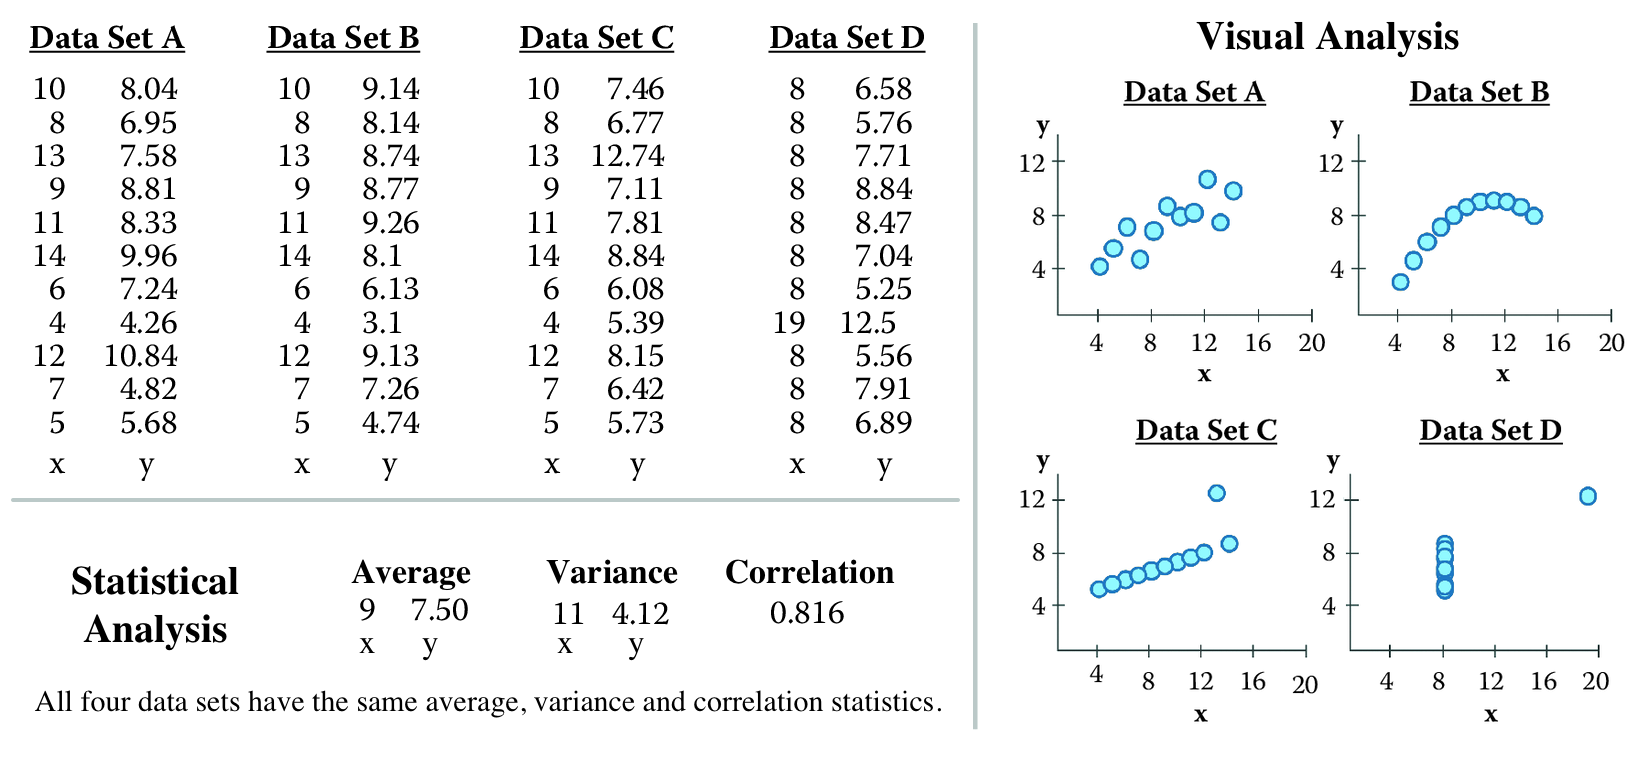
\includegraphics[width=0.9\linewidth]{ChapterViz/figures/fig9-1-new} 

}

\caption{Adapted from Anscombe`s quartet [@anscombe1973graphs]}\label{fig:fig9-1}
\end{figure}

In broad terms, visualizations are used either to present results or for
analysis and open-ended exploration. This chapter provides an overview
of how modern information visualization, or visual data mining, can be
used to in the context of big data.

\section{Developing effective visualizations}\label{sec:viz-2}

The effectiveness of a visualization depends on both analysis needs and
design goals. Sometimes, questions about the data are known in advance;
in other cases, the goal may be to explore new data sets, generate
insights, and answer questions that are unknown before starting the
analysis. The design, development, and evaluation of a visualization is
guided by understanding the background and goals of the target audience
(see Box \protect\hyperlink{box:viz1}{Effective
visualizations}\footnote{See Chapters
  \protect\hyperlink{chap:web}{Working with Web Data and APIs},
  \protect\hyperlink{chap:link}{Record Linkage},
  \protect\hyperlink{chap:db}{Databases}, and
  \protect\hyperlink{chap:parallel}{Scaling up through Parallel and
  Distributed Computing} for an overview of collecting, merging,
  storing, and processing data sets.}).

\begin{center}\rule{0.5\linewidth}{\linethickness}\end{center}

\textbf{Box: Effective visualizations}

The development of an effective visualization is a continous process
that generally includes the following activities:

\begin{itemize}
\item
  Specify user needs, tasks, accessibility requirements and criteria for
  success.
\item
  Prepare data (clean, transform).
\item
  Design visual representations.
\item
  Design interaction.
\item
  Plan sharing of insights, provenance.
\item
  Prototype/evaluate, including usability testing.
\item
  Deploy (monitor usage, provide user support, manage revision process).
\end{itemize}

\begin{center}\rule{0.5\linewidth}{\linethickness}\end{center}

If the goal is to present results, there is a wide spectrum of users and
a wide range of options. If the audience is broad, then
\emph{infographics} can be developed by graphic designers, as described
in classic texts (see Few (\protect\hyperlink{ref-few2009now}{2009});
Tufte (\protect\hyperlink{ref-edward2001visual}{2001}); Tufte
(\protect\hyperlink{ref-edward2006beauty}{2006}) or the examples
compiled by Harrison, Reinecke, and Chang
(\protect\hyperlink{ref-harrison2015infographic}{2015}); Keshif (n.d.)).
If, on the other hand, the audience comprises domain experts interested
in monitoring the overview status of dynamic processes on a continuous
basis, monitoring \emph{dashboards} with no or little interactivity can
be used. Examples include the monitoring of sales, or the number of
tweets about people, or symptoms of the flu and how they compare to a
baseline (Few \protect\hyperlink{ref-few2013information}{2013}). Such
dashboards, composed of multiple charts of different operational data,
can increase situational awareness so that problems can be noticed and
solved early and better decisions can be made with up-to-date
information.

Another goal of visualization is to enable \emph{interactive exploratory
analysis}. This approach goes beyond a visual snapshot of data for
presentation, and provides many windows into different parts and
relationships within data on demand. Tailor-made solutions can focus on
specific querying and navigation tasks given a specific data. For
example, the BabyNameVoyager
(\url{http://www.babynamewizard.com/voyager/}) lets users type in a name
and see a graph of its popularity over the past century. With each
letter typed, the page filters baby names starting with the input (such
as Joan, Joyce and John for input ``Jo'').''

\begin{figure}

{\centering 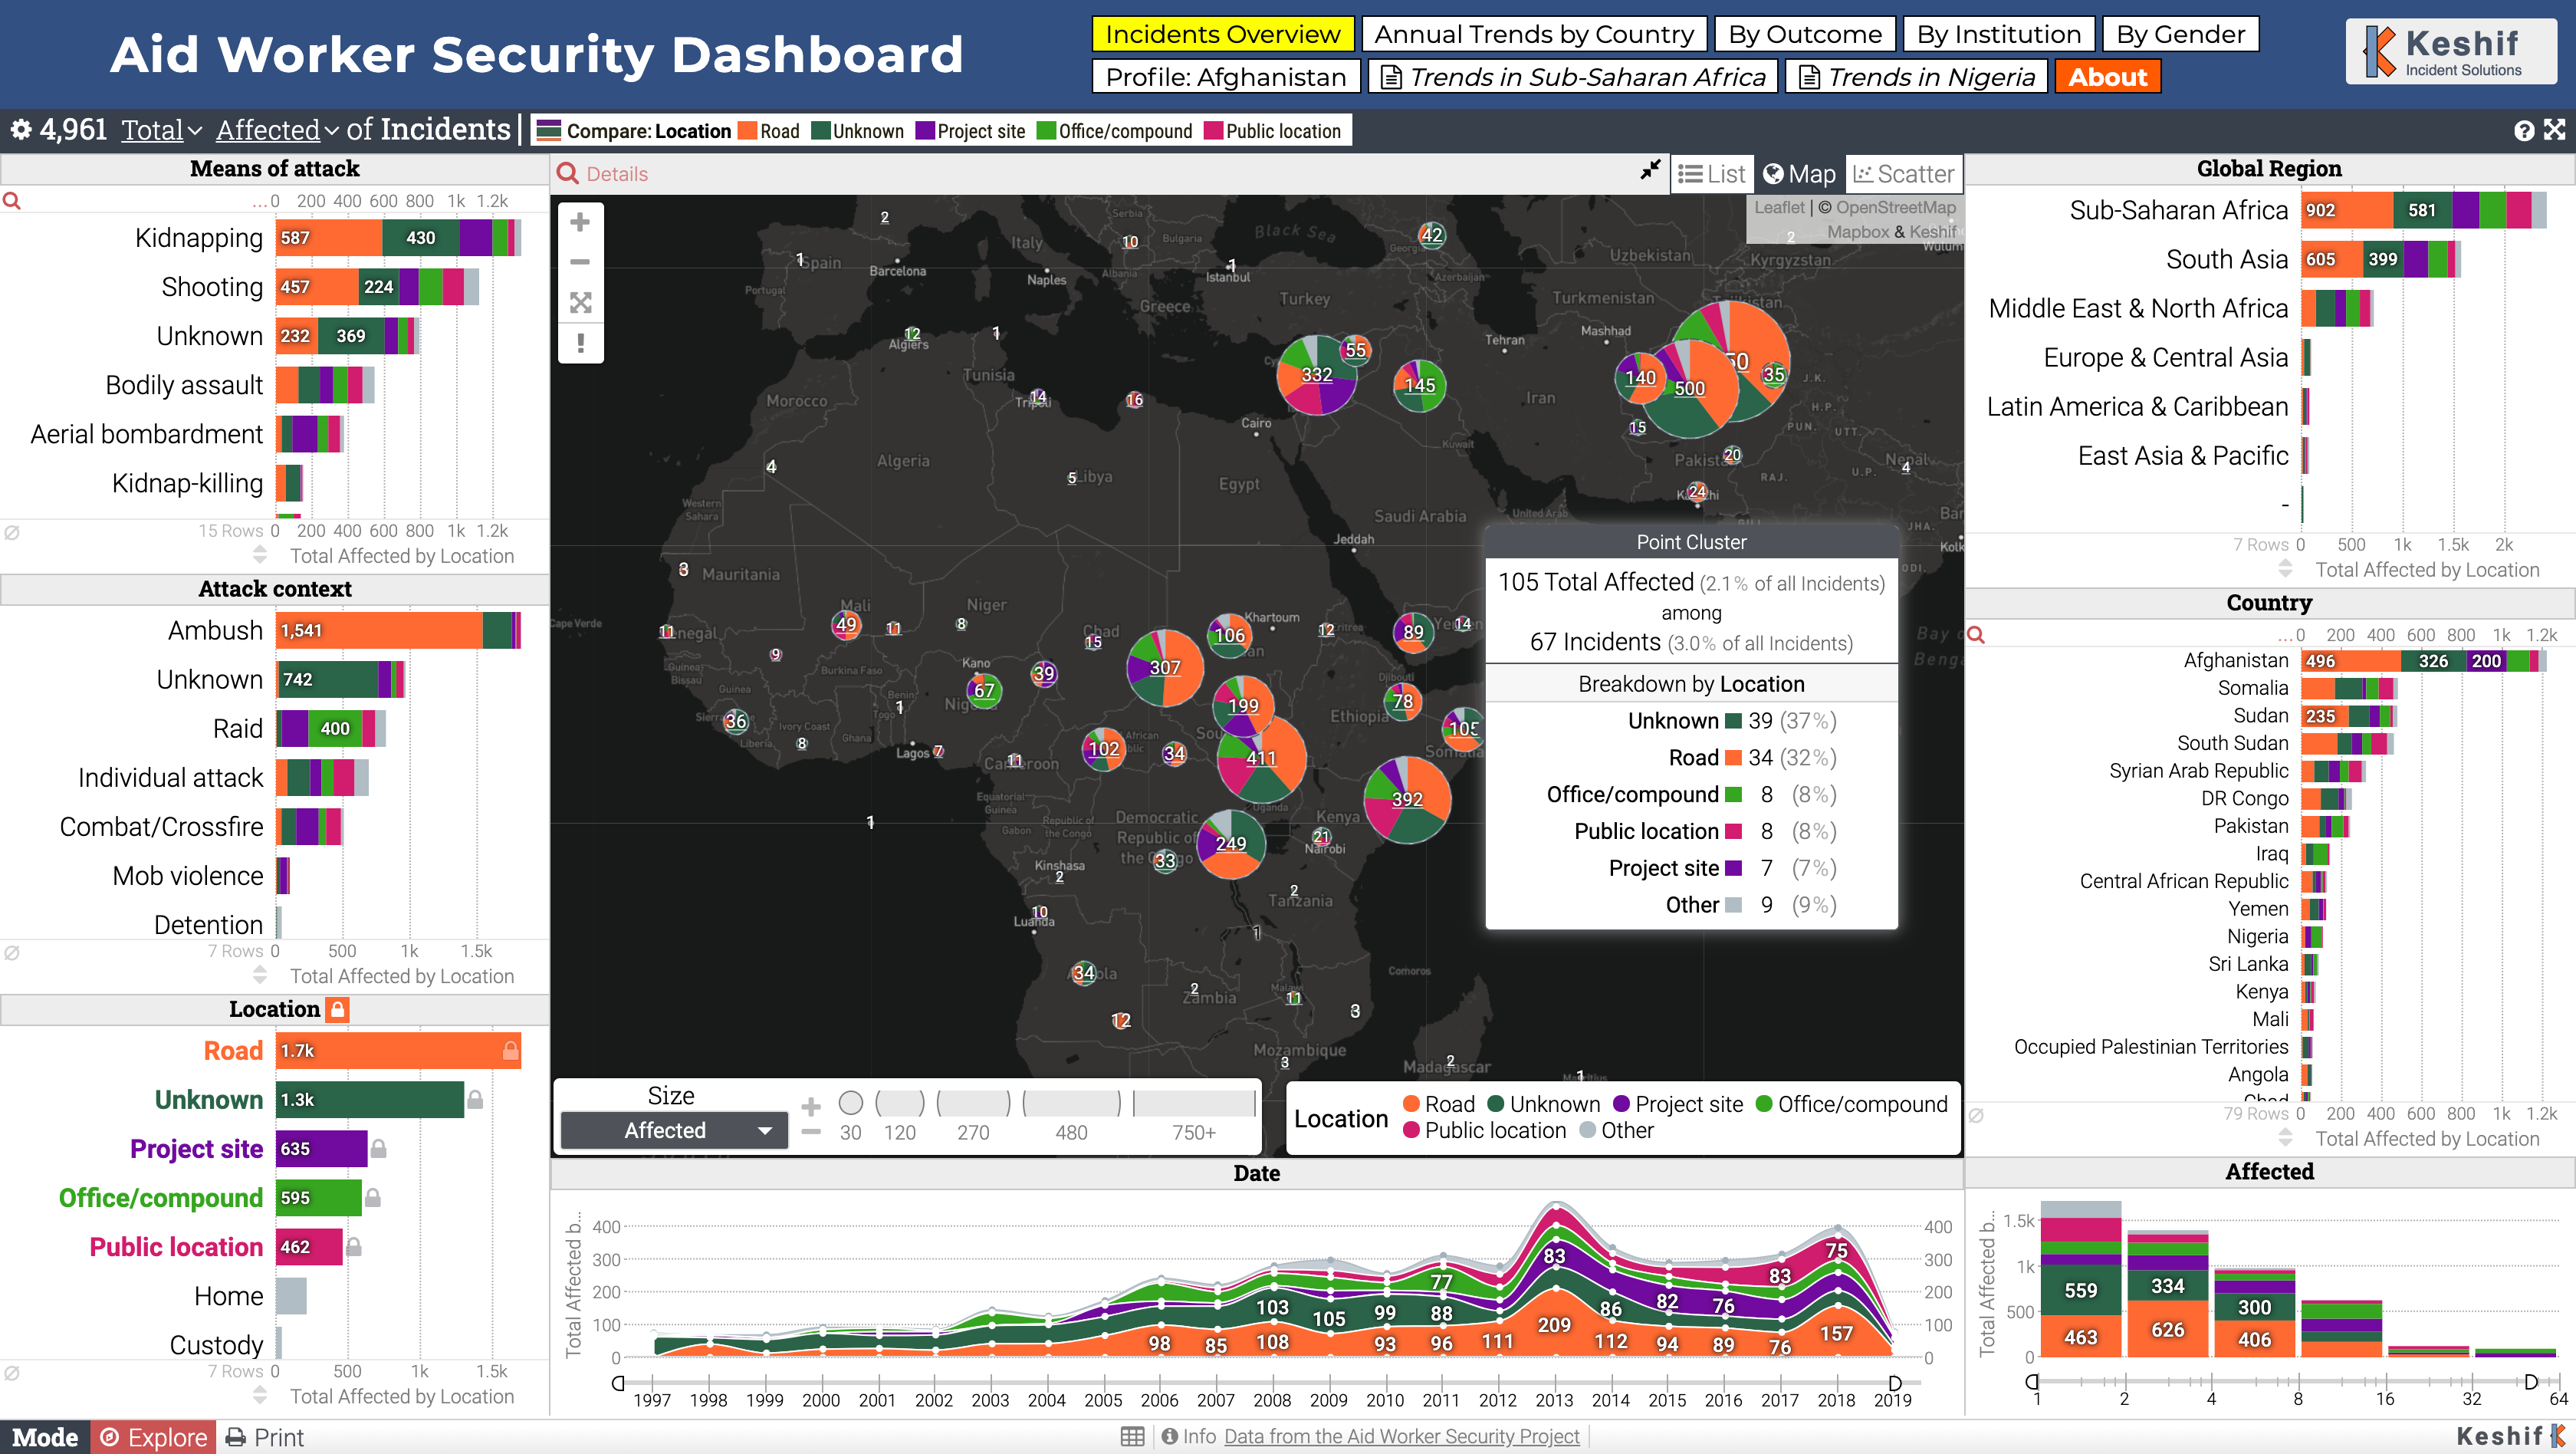
\includegraphics[width=0.9\linewidth]{ChapterViz/figures/fig9-2a-new} 

}

\caption{Aid Worker Security Incidents Analysis Dashboard (https://gallery.keshif.me/AidWorkerSecurity)}\label{fig:fig9-2a}
\end{figure}

In addition, detailed aspects of a dataset can be made explorable by
advanced data querying, navigation and view options. Figure
\ref{fig:fig9-2a} shows an interactive dashboard that visualizes the
data from the Humanitarian Outcomes' Aid Worker Security Database
(\url{https://aidworkersecurity.org/}). In this example, the event point
locations are clustered on a map, and surrounding charts show trends in
attack means, context, location types, region, country, as well as event
date and the number of affected people. This view also presents a
breakdown of data by location type, shown using color, includes
contextual tooltips that provide details on a geographic cluster of
points. Additional shortcuts on top allow navigation to key alternative
insights as a storytelling tool.

\begin{figure}

{\centering 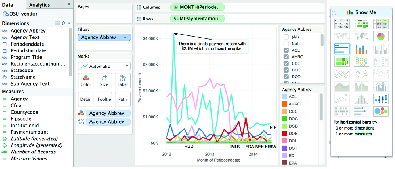
\includegraphics[width=0.9\linewidth]{ChapterViz/figures/fig9-3a} 

}

\caption{Charting interface of Tableau}\label{fig:fig9-3a}
\end{figure}

\begin{figure}

{\centering 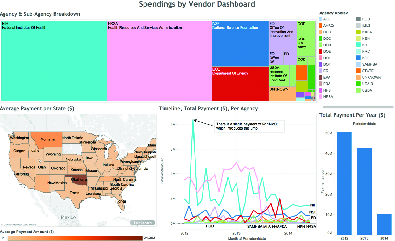
\includegraphics[width=0.9\linewidth]{ChapterViz/figures/fig9-3b} 

}

\caption{A treemap visualization of agency and sub-agency spending breakdown}\label{fig:fig9-3b}
\end{figure}

To create interactive charts and dashboards from new datasets for
analysis, products and tools, such as Tableau, PowerBI, Keshif, and
others (see Section \protect\hyperlink{sec:viz-6}{Resources}), offer a
range of chart types with various parameters, as well as visual design
environments that allow combining and sharing these charts in potent
dashboards. For example, Figure \ref{fig:fig9-3a} shows the charting
interface of Tableau on a transaction data set. The left-hand panel
shows the list of attributes associated with vendor transactions for a
given university. The visualization (center) is constructed by placing
the month of spending in chart columns, and the sum of payment amount on
the chart row, with data encoded using line mark type. Agencies are
broken down by color mapping. The agency list, to the right, allows
filtering the agencies, which can be used to simplify the chart view. A
peak in the line chart is annotated with an explanation of the spike. On
the rightmost side, the Show Me panel suggests the applicable chart
types potentially appropriate for the selected attributes. This chart
can be combined with other charts focusing on other aspects in
interactive dashboards. Figure \ref{fig:fig9-3b} shows a treemap
(Johnson and Shneiderman \protect\hyperlink{ref-johnson1991tree}{1991})
for agency and sub-agency spending breakdown, combined with a map
showing average spending per state. Oklahoma state stands out with few
but large expenditures. Mousing-over Oklahoma reveals details of these
expenditures. An additional histogram provides an overview of spending
change across three years.

Creating effective visualizations requires careful consideration of many
components. Data values may be encoded using one or more visual
elements, like position, length, color, angle, area, and texture (Figure
\ref{fig:fig9-4}; see also Cleveland and McGill
(\protect\hyperlink{ref-cleveland1984graphical}{1984}); Tufte
(\protect\hyperlink{ref-edward2001visual}{2001})). Each of these can be
organized in a multitude of ways, discussed in more detail by Munzner
(\protect\hyperlink{ref-munzner2014visualization}{2014}). In addition to
visual data encoding, units for axes, labels, and legends need to be
provided as well as explanations of the mappings when the design is
unconventional. A visually compelling example is ``how to read this
data'' section of ``A world of Terror'' project by Periscopic
(\url{https://terror.periscopic.com/}).

Annotations or comments can be used to guide viewer attention and to
describe related insights. Providing attribution and data source, where
applicable, is an ethical practice that also enables validating data,
and promotes reuse to explore new perspectives.

\begin{figure}

{\centering 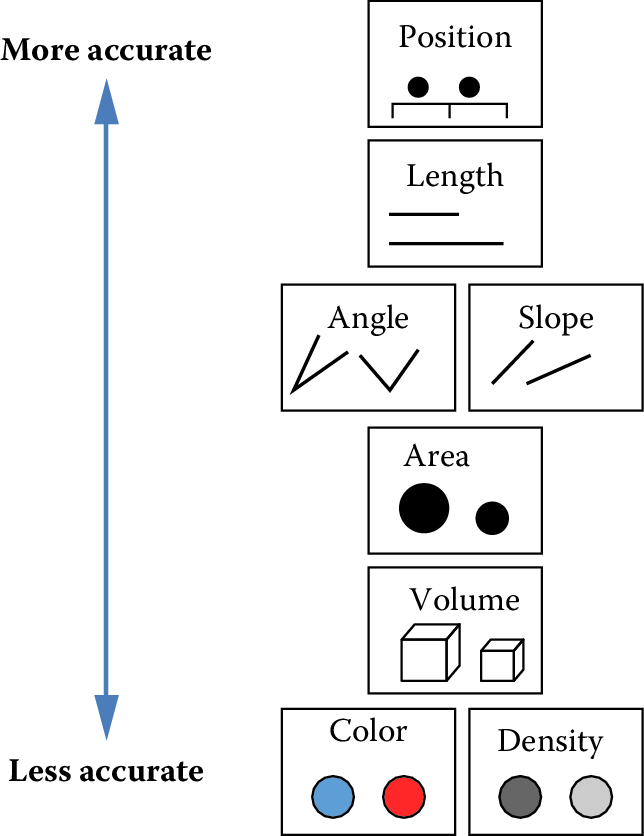
\includegraphics[width=0.5\linewidth]{ChapterViz/figures/fig9-4} 

}

\caption{Visual elements described by MacKinlay [@mackinlay1986automating]}\label{fig:fig9-4}
\end{figure}

The following is a short list of guidelines: provide immediate feedback
upon interaction with the visualization; generate tightly coupled views
(i.e., so that selection in one view updates the others); and use a high
``data to ink ratio'' (Tufte
\protect\hyperlink{ref-edward2001visual}{2001}). Use color carefully and
ensure that the visualization is truthful (e.g., watch for perceptual
biases or distortion). Avoid use of three-dimensional representations or
embellishments, since comparing 3D volumes is perceptually challenging
and occlusion is a problem. Labels and legends should be meaningful,
novel layouts should be carefully explained, and online visualizations
should adapt to different screen sizes. For extended and in-depth
discussions, see various textbooks (Few
\protect\hyperlink{ref-few2009now}{2009}; Kirk
\protect\hyperlink{ref-kirk2012data}{2012}; Ward, Grinstein, and Keim
\protect\hyperlink{ref-ward2010interactive}{2010}; Munzner
\protect\hyperlink{ref-munzner2014visualization}{2014}; Tufte
\protect\hyperlink{ref-edward2001visual}{2001}; Tufte
\protect\hyperlink{ref-edward2006beauty}{2006}).

We provide a summary of the basic tasks that users typically perform
during visual analysis of data in the next section.

\section{A data-by-tasks taxonomy}\label{sec:viz-3}

We give an overview of visualization approaches for six common data
types: multivariate, spatial, temporal, hierarchical, network, and text
(Shneiderman and Plaisant
\protect\hyperlink{ref-shneiderman2015sharpening}{2015}). For each data
type listed in this section, we discuss its distinctive properties, the
common analytical questions, and examples. Real-life data sets often
include multiple data types coming from multiple sources. Even a single
data source can include a variety of data types. For example, a single
data table of countries (as rows) can have a list of attributes with
varying types: the growth rate in the last 10 years (one observation per
year, time series data), their current population (single numerical
data), the amount of trade with other countries (networked/linked data),
and the top 10 exported products (if grouped by industry, hierarchical
data).

In addition to common data types, Box
\protect\hyperlink{box:viz2}{Tasks} provides an overview of common tasks
for visual data analysis, which can be applied across different data
types based on goals and types of visualizations.

\begin{center}\rule{0.5\linewidth}{\linethickness}\end{center}

\textbf{Box: A task categorization for visual data analysis}

Select/Query

\begin{itemize}
\tightlist
\item
  Filter to focus on a subset of the data
\item
  Retrieve details of item
\item
  Brush linked selections across multiple charts
\item
  Compare across multiple selections
\end{itemize}

Navigate

\begin{itemize}
\tightlist
\item
  Scroll along a dimension (1D)
\item
  Pan along two dimensions (2D)
\item
  Zoom along the third dimension (3D)
\end{itemize}

Derive

\begin{itemize}
\tightlist
\item
  Aggregate item groups and generate characteristics
\item
  Cluster item groups by algorithmic techniques
\item
  Rank items to define ordering
\end{itemize}

Organize

\begin{itemize}
\tightlist
\item
  Select chart type and data encodings to organize data
\item
  Layout multiple components or panels in the interface
\end{itemize}

Understand

\begin{itemize}
\tightlist
\item
  Observe distributions
\item
  Compare items and distributions
\item
  Relate items and patterns
\end{itemize}

Communicate

\begin{itemize}
\tightlist
\item
  Annotate findings
\item
  Share results
\item
  Trace action histories
\end{itemize}

\begin{center}\rule{0.5\linewidth}{\linethickness}\end{center}

Interactive visualization design should also consider the devices where
data will be viewed and interacted. Conventionally, visualizations have
been designed for mouse and keyboard interaction on desktop computers.
However, a wider range of device forms, such as mobile devices with
small displays and touch interaction, is becoming common. Creating
visualizations for new forms requires special care, though basic design
principles such as ``less is more'' still apply.

\subsection{Multivariate data}\label{sec:viz-2.1}

In common tabular data, each record (row) has a list of attributes
(columns), whose value is mostly categorical or numerical. The analysis
of multivariate data with basic categorical and interval types aims to
understand patterns within and across data attributes. Given a larger
number of attributes, one of the challenges in data exploration and
analytics is to select the attributes and relations to focus on.
Expertise in the data domain can be helpful for targeting relevant
attributes.

Multivariate data can be presented in multiple forms of charts depending
on the data and relations being explored. One-dimensional (1D) charts
present data on a single axis only. An example is a \emph{box-plot},
which shows quartile ranges for numerical data. So-called 1.5D charts
list the range of possible values on one axis, and describe a
measurement of data on the other. \emph{Bar charts} are a ubiquitous
chart type that can effectively visualize numeric data, for example, a
numeric grade per student, or grade average for aggregated student
groups by gender. Records can also be grouped over numerical ranges such
as sales price, and bars can show the number of items in each grouping,
which generates a \emph{histogram} chart. Two-dimensional charts, such
as scatterplots, plot data along two attributes, such as
\emph{scatterplots}. Matrix (grid) charts can also be used to show
relations between two attributes. \emph{Heatmaps} visualize each matrix
cell using color to represent its value. \emph{Correlation matrices}
show the relation between attribute pairs.

To show relations of more than two attributes (3D+), one option is to
use additional visual encodings in a single chart, for example, by
adding point size/shape as a data variable in scatterplots. Another
option is to use alternative visual designs that can encode multiple
relations within a single chart. For example, a \emph{parallel
coordinate plot} (Inselberg \protect\hyperlink{ref-inselberg2009}{2009})
has multiple parallel axes, each one representing an attribute; each
record is shown as connected lines passing through the record's values
on each attribute. Charts can also show part-of-whole relations using
appropriate mappings based on subdividing the chart space, such as
stacked charts or pie charts.

Finally, another approach to analyzing multidimensional data is to use
clustering algorithms to identify similar items. Clusters are typically
represented as a tree structure (see Section
\protect\hyperlink{sec:viz-2.5}{Hierarchical data}). For example,
\(k\)-means clustering starts by users specifying how many clusters to
create; the algorithm then places every item into the most appropriate
cluster. Surprising relationships and interesting outliers may be
identified by these techniques on mechanical analysis algorithms.
However, such results may require more effort to interpret.

\subsection{Spatial data}\label{sec:viz-2.2}

Spatial data convey a physical context, commonly in a 2D space, such as
geographical maps or floor plans. Several of the most examples of
information visualization include maps, from the 1861 representation of
Napoleon's ill-fated Russian campaign by Minard (popularized by Tufte
Tufte (\protect\hyperlink{ref-edward2001visual}{2001}) and Kraak Kraak
(\protect\hyperlink{ref-Kraak2014}{2014})) to the interactive HomeFinder
application that introduced the concept of dynamic queries (Ahlberg,
Williamson, and Shneiderman
\protect\hyperlink{ref-ahlberg1992dynamic}{1992}). The tasks include
finding adjacent items, regions containing certain items or with
specific characteristics, and paths between items---and performing the
basic tasks listed in Box \protect\hyperlink{box:viz1}{Effective
visualizations}.

The primary form of visualizing spatial data is \emph{maps}. In
\emph{choropleth maps}, color encoding is used to add represent one data
attribute. \emph{Cartograms} aim to encode the attribute value with the
size of regions by distorting the underlying physical space. \emph{Tile
grid maps} reduce each spatial area to a uniform size and shape (e.g., a
square) so that the color-coded data are easier to observe and compare,
tile grid maps convert each spatial region to a fixed shape, such as a
square tile and arrange these tiles to approximate and maintain relative
physical positions of the regions (DeBelius
\protect\hyperlink{ref-DeBelius2015}{2015}; Stanford Visualization
Group, n.d.). Grid maps also make selection of smaller areas (such as
small cities or states) easier. \emph{Contour (isopleth) maps} connect
areas with similar measurements and color each one separately.
\emph{Network maps} aim to show network connectivity between locations,
such as flights to/from many regions of the world. Spatial data can be
also presented with a nonspatial emphasis (e.g., as a hierarchy of
continents, countries, and cities, such as by using a treemap chart.).

\begin{figure}

{\centering 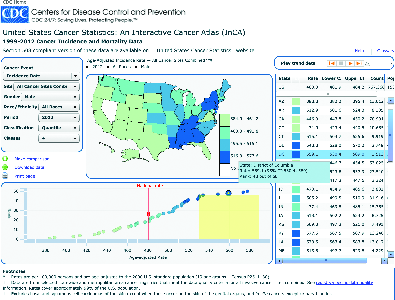
\includegraphics[width=0.9\linewidth]{ChapterViz/figures/fig9-5} 

}

\caption{The US Cancer Atlas [@usca]. Interface based on [@maceachren2008design]}\label{fig:fig9-5}
\end{figure}

Maps are commonly combined with other visualizations. For example, in
Figure \ref{fig:fig9-5}, the US Cancer Atlas combines a map showing
patterns across states on one attribute, with a sortable table providing
additional statistical information and a scatterplot that allows users
to explore correlations between attributes. Figures \ref{fig:fig9-2a}
and \ref{fig:fig9-3b} also demonstrate the use of different map designs
in the context of larger analytical solutions.

\subsection{Temporal data}\label{sec:viz-2.4}

Time is the unique dimension in our physical world that steadily flows
forward. While we cannot control time, we frequently record it as a
point or an interval. Figures \ref{fig:fig9-2a} and \ref{fig:fig9-3a}
exemplify line charts that show trends over multiple years, with each
single line representing a subset of the data for cross-comparison of
temporal trends. Temporal data also has multiple levels of
representation (year, month, day, hour, minute, and so on) with
irregularities (leap year, different days per month, etc.). As we
measure time based on cyclic events in nature (day/night), our
representations are also commonly cyclic. For example, January follows
December (first month follows last). This cyclic nature can be captured
by circular visual encodings, such as the the conventional clock with
hour, minute, and second hands.

Time series data (Figures \ref{fig:fig9-6} and \ref{fig:fig9-7})
describe values measured at regular intervals, such as stock market or
weather data. The focus of analysis is to understand temporal trends and
anomalies, querying for specific patterns, or prediction. To show
multiple time-series trends across different data categories in a very
compact chart area, each trend can be shown with small height using a
multi-layered color approach, creating horizon graphs. While
perceptually effective after learning to read its encoding, this chart
design may not be appropriate for audiences who may lack such training
or familiarity.

\begin{figure}

{\centering 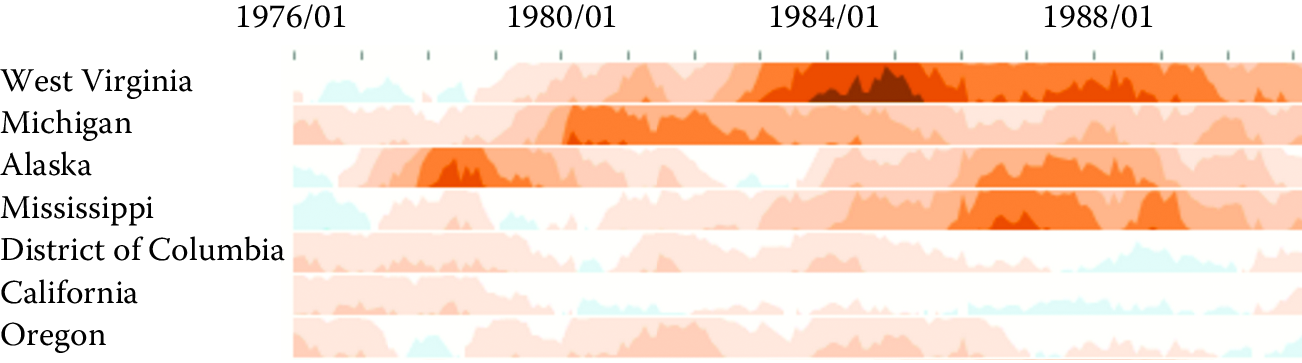
\includegraphics[width=0.9\linewidth]{ChapterViz/figures/fig9-6} 

}

\caption{Horizon graphs used to display time series}\label{fig:fig9-6}
\end{figure}

\begin{figure}

{\centering 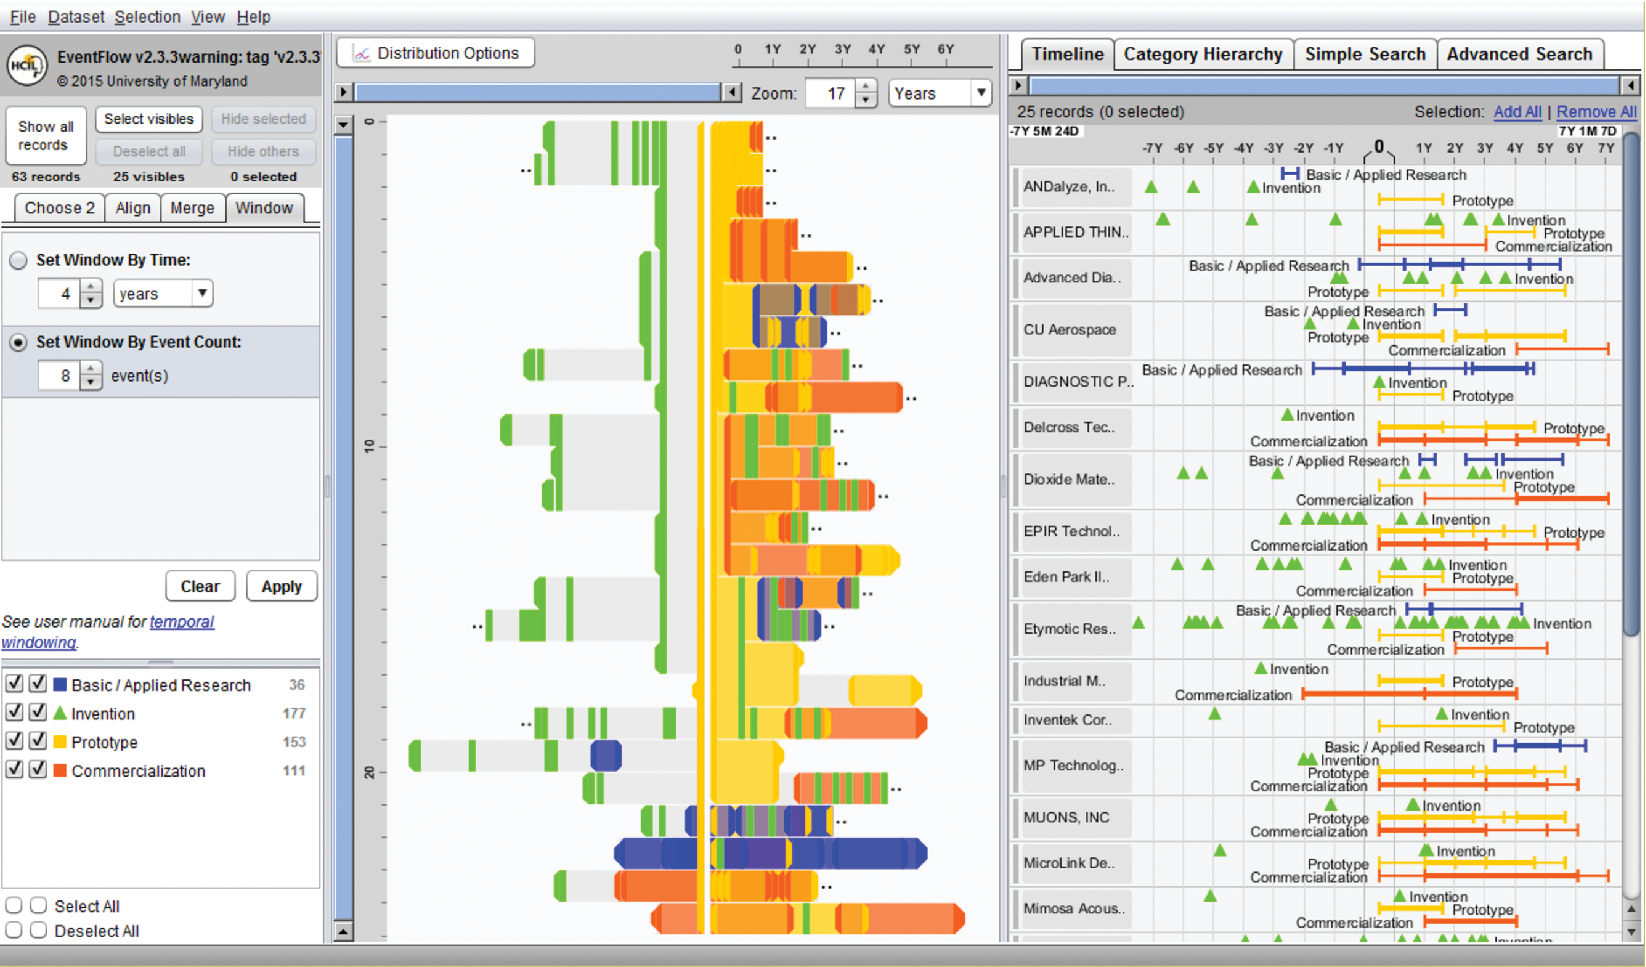
\includegraphics[width=0.9\linewidth]{ChapterViz/figures/fig9-7} 

}

\caption{EventFlow (https://hcil.umd.edu/eventflow/) is used to visualize sequences of innovation activities by Illinois companies. Created with EventFlow; data sources include NIH, NSF, USPTO, SBIR. Image created by C. Scott Dempwolf, used with permission}\label{fig:fig9-7}
\end{figure}

Another form of temporal analysis is understanding sequences of events.
The study of human activity often includes analyzing event sequences.
For example, students' records include events such as attending
orientation, getting a grade in a class, going on internship, and
graduation. In the analysis of event sequences, finding the most common
patterns, spotting rare ones, searching for specific sequences, or
understanding what leads to particular types of events is important
(e.g., what events lead to a student dropping out, precede a medical
error, or a company filing bankruptcy). Figure \ref{fig:fig9-7} shows
EventFlow used to visualize sequences of innovation activities by
Illinois companies. Activity types include research, invention,
prototyping, and commercialization. The timeline (right panel) shows the
sequence of activities for each company. The overview panel (center)
summarizes all the records aligned by the first prototyping activity of
the company. In most of the sequences shown here, the company's first
prototype is preceded by two or more patents with a lag of about a year.

\hypertarget{sec:viz-2.5}{\subsection{Hierarchical
data}\label{sec:viz-2.5}}

Data are often organized in a hierarchical fashion. Each item appears in
one grouping (e.g., like a file in a folder), and groups can be grouped
to form larger groups (e.g., a folder within a folder), up to the root
(e.g., a hard disk). Items, and the relations between items and their
grouping, can have their own attributes. For example, the National
Science Foundation is organized into directorates and divisions, each
with a budget and a number of grant recipients.

Analysis may focus on the structure of the relations, by questions such
as ``how deep is the tree?'', ``how many items does this branch have?'',
or ``what are the characteristics of one branch compared to another?''
In such cases, the most appropriate representation is usually a
node-link diagram (Plaisant, Grosjean, and Bederson
\protect\hyperlink{ref-plaisant2002spacetree}{2002}; Card and Nation
\protect\hyperlink{ref-card2002degree}{2002}). In Figure
\ref{fig:fig9-8}, Spacetree is used to browse a company organizational
chart. Since not all the nodes of the tree fit on the screen, we see an
iconic representation of the branches that cannot be displayed,
indicating the size of each branch. As the tree branches are opened or
closed, the layout is updated with smooth multiple-step animations to
help users remain oriented.

When the structure is less important but the attribute values of the
leaf nodes are of primary interest, treemaps, a space-filling approach,
are preferable as they can show arbitrary-sized trees in a fixed
rectangular space and map one attribute to the size of each rectangle
and another to color. For example, Figure \ref{fig:fig9-9} shows the
Finviz treemap that helps users monitor the stock market. Each stock is
shown as a rectangle. The size of the rectangle represents market
capitalization, and color indicates whether the stock is going up or
down. Treemaps are effective for situation awareness: we can see that
today is a fairly bad day as most stocks are red (i.e., down). Stocks
are organized in a hierarchy of industries, allowing users to see that
``healthcare technology'' is not doing as poorly as most other
industries. Users can also zoom on healthcare to focus on that industry.

\begin{figure}

{\centering 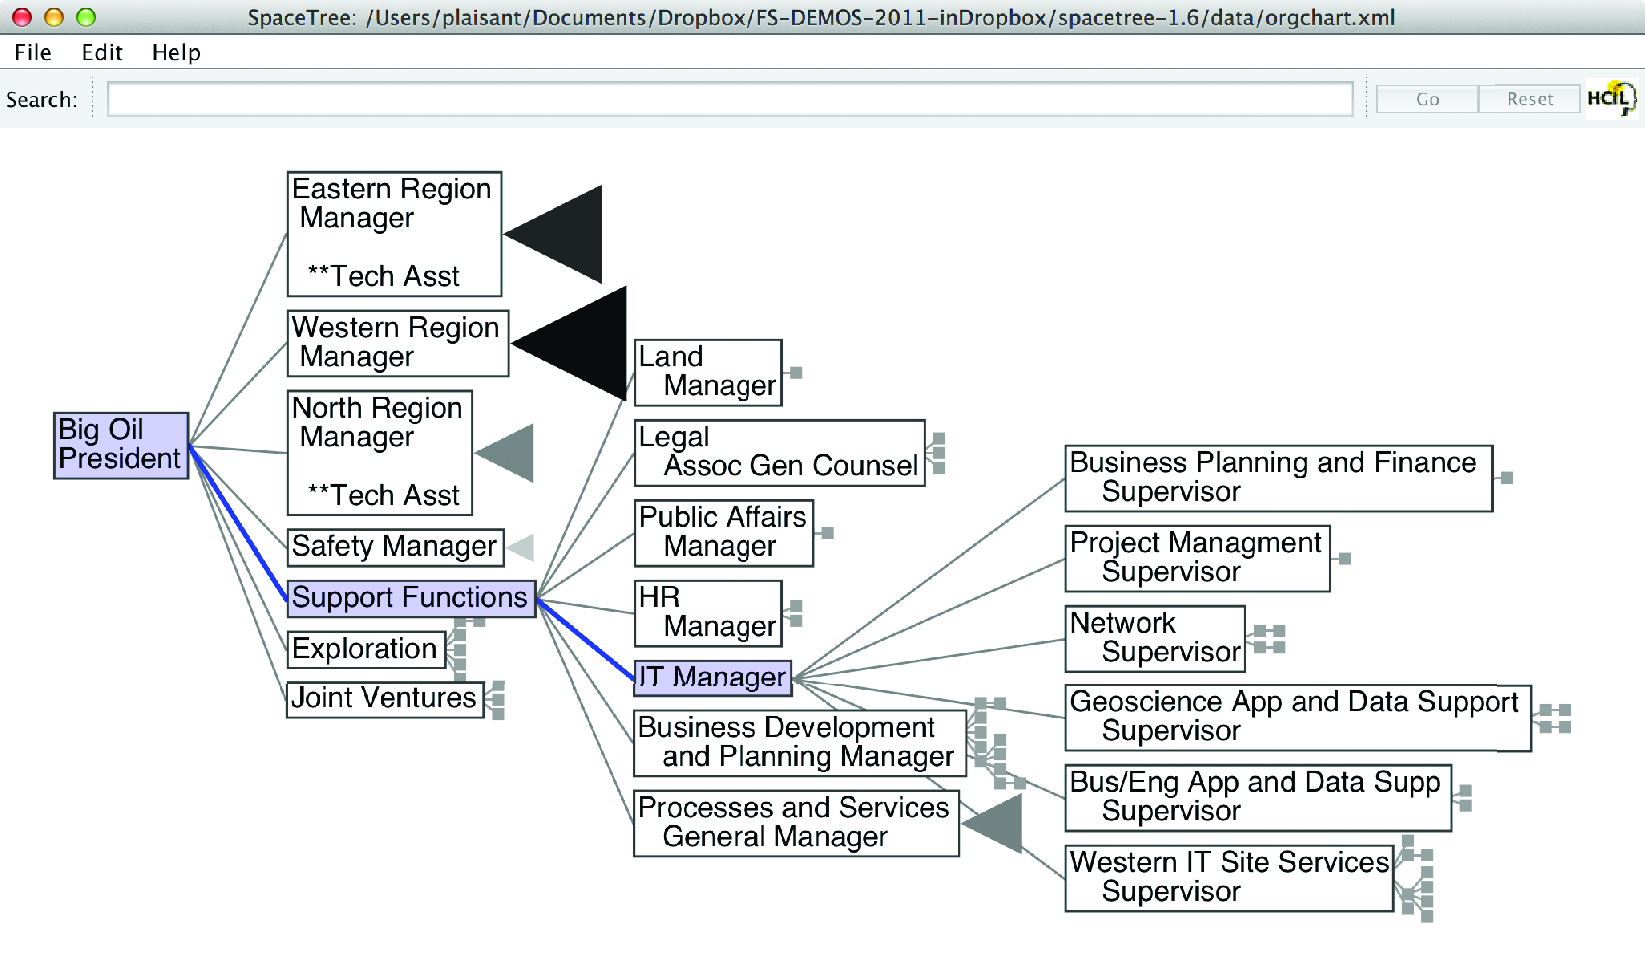
\includegraphics[width=0.9\linewidth]{ChapterViz/figures/fig9-8} 

}

\caption{SpaceTree (http://www.cs.umd.edu/hcil/spacetree/)}\label{fig:fig9-8}
\end{figure}

\begin{figure}

{\centering 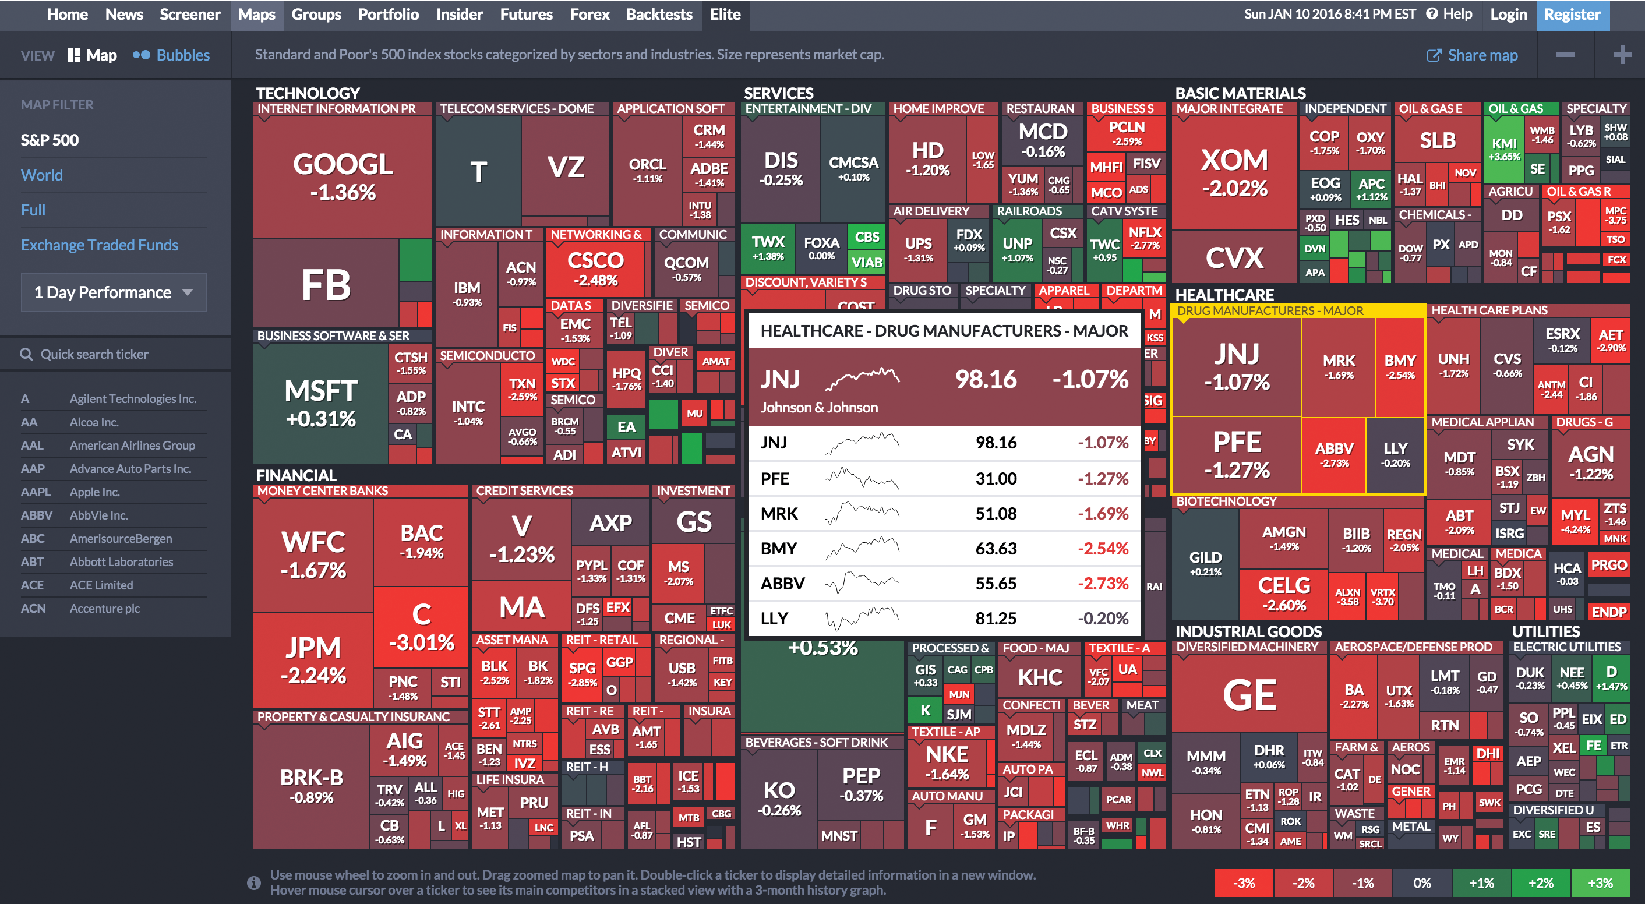
\includegraphics[width=0.9\linewidth]{ChapterViz/figures/fig9-9} 

}

\caption{The Finviz treemap helps users monitor the stock market (https://www.finviz.com/)}\label{fig:fig9-9}
\end{figure}

\subsection{Network data}\label{sec:viz-2.6}

\begin{figure}

{\centering 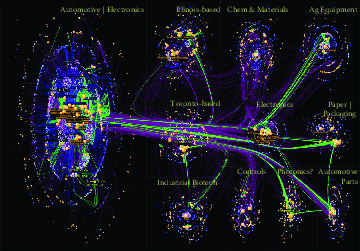
\includegraphics[width=0.9\linewidth]{ChapterViz/figures/fig9-10} 

}

\caption{NodeXL showing innovation networks of the Great Lakes manufacturing region. Created with NodeXL. Data source: USPTO. Image created by C. Scott Dempwolf, used with permission}\label{fig:fig9-10}
\end{figure}

Network data encode relationships between items\footnote{See Chapter
  \protect\hyperlink{chap:networks}{Networks: The Basics}.}: for
example, social connection patterns (friendships, follows and reposts,
etc.), travel patterns (such as trips between metro stations), and
communication patterns (such as emails). The network overviews attempt
to reveal the structure of the network, show clusters of related items
(e.g., groups of tightly connected people), and allow the path between
items to be traced. Analysis can also focus on attributes of the items
and the links in between, such as age of people in communication or the
average duration of communications.

\begin{figure}

{\centering 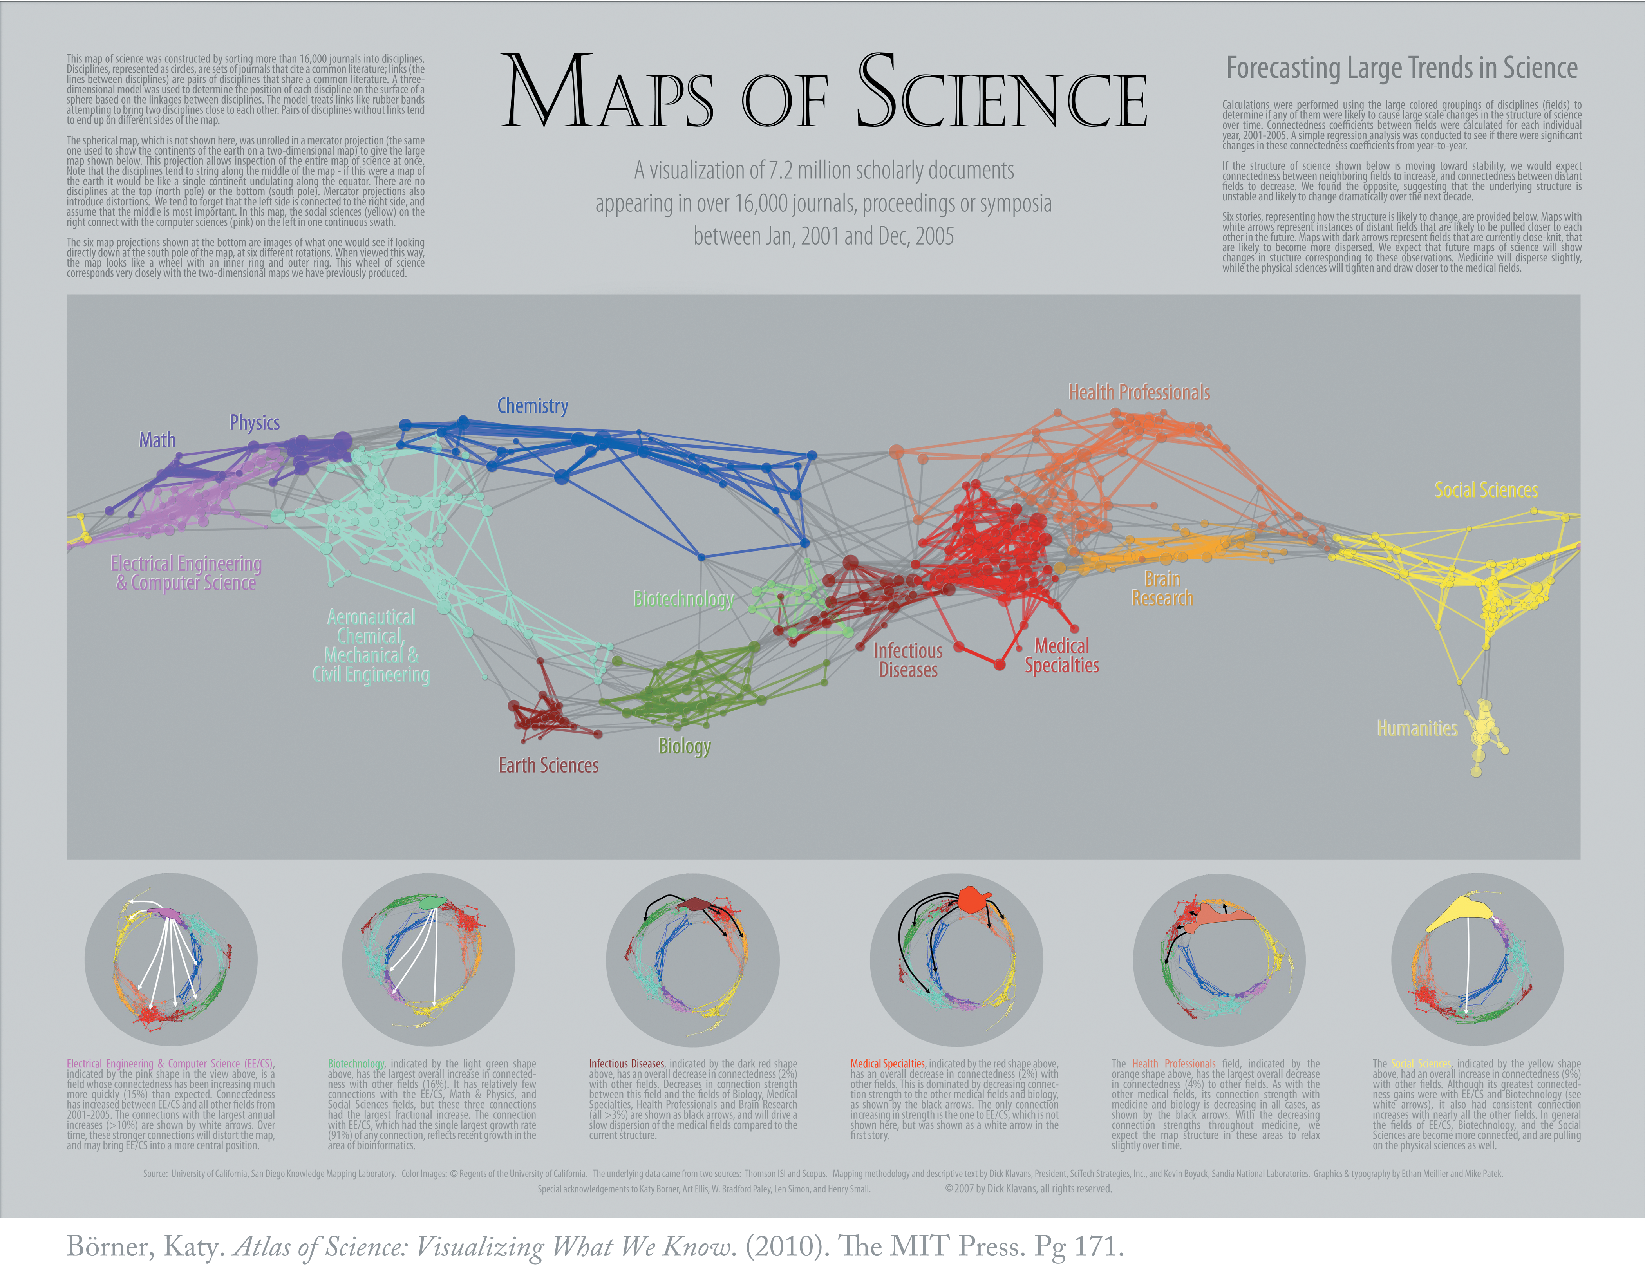
\includegraphics[width=0.9\linewidth]{ChapterViz/figures/fig9-10b} 

}

\caption{An example from "Maps of Science: Forecasting Large Trends in Science," 2007, The Regents of the University of California, all rights reserved [@borner2010atlas]}\label{fig:fig9-10b}
\end{figure}

Node-link diagrams are the most common representation of network
structures and overviews (Figures \ref{fig:fig9-10} and
\ref{fig:fig9-10b}, and may use linear (arc), circular, or force-
directed layouts for positioning the nodes (items). Matrices or grid
layouts are also a valuable way to represent networks (Henry and Fekete
\protect\hyperlink{ref-henry2006matrixexplorer}{2006}). Hybrid solutions
have been proposed, with powerful ordering algorithms to reveal clusters
(Hansen, Shneiderman, and Smith
\protect\hyperlink{ref-hansen2010analyzing}{2010}). A major challenge in
network data exploration is in dealing with larger networks where nodes
and edges inevitably overlap by virtue of the underlying network
structure, and where aggregation and filtering may be needed before
effective overviews can be presented to users.

Figure \ref{fig:fig9-10} shows the networks of inventors (white) and
companies (orange) and their patenting connections (purple lines) in the
network visualization NodeXL. Each company and inventor is also
connected to a location node (blue = USA; yellow = Canada). Green lines
are weak ties based on patenting in the same class and subclass, and
they represent potential economic development leads. The largest of the
technology clusters are shown using the \emph{group-in-a-box} layout
option, which makes the clusters more visible. Note the increasing level
of structure moving from the cluster in the lower right to the main
cluster in the upper left. NodeXL is designed for interactive network
exploration; many controls (not shown in the figure) allow users to zoom
on areas of interest or change options. Figure \ref{fig:fig9-10b} shows
an example of network visualization on science as a topic used for data
presentation in a book and a traveling exhibit. Designed for print
media, it includes a clear title and annotations and shows a series of
topic clusters at the bottom with a summary of the insights gathered by
analysts.

\subsection{Text data}\label{sec:viz-2.7}

Text is usually preprocessed (for word/paragraph counts, sentiment
analysis, categorization, etc.) to generate metadata about text
segments, which are then visualized\footnote{See Chapter
  \protect\hyperlink{chap:text}{Text Analysis} for text analysis
  approaches.}. Simple visualizations like tag clouds display statistics
about word usage in a text collection, or can be used to compare two
collections or text segments. While visually appealing, they can easily
be misinterpreted and are often replaced by word indexes sorted by some
count of interest. Specialized visual text analysis tools combine
multiple visualizations of data extracted from the text collections,
such as matrices to see relations, network diagrams, or parallel
coordinates to see entity relationships (e.g., between what, who, where,
and when). Timelines can be mapped to the linear dimension of text.
Figure \ref{fig:fig9-11} shows an example using Jigsaw (Stasko, Görg,
and Liu \protect\hyperlink{ref-stasko2008jigsaw}{2008}) for the
exploration of car reviews. Entities have been extracted automatically
(in this case make, model, features, etc.), and a cluster analysis has
been performed, visualized in the bottom right. A separate view
(rightmost) allows analysts to review links between entities. Another
view allows traversing word sequences as a tree. Reading original
documents is critical, so all the visualization elements are linked to
the corresponding text.

\begin{figure}

{\centering 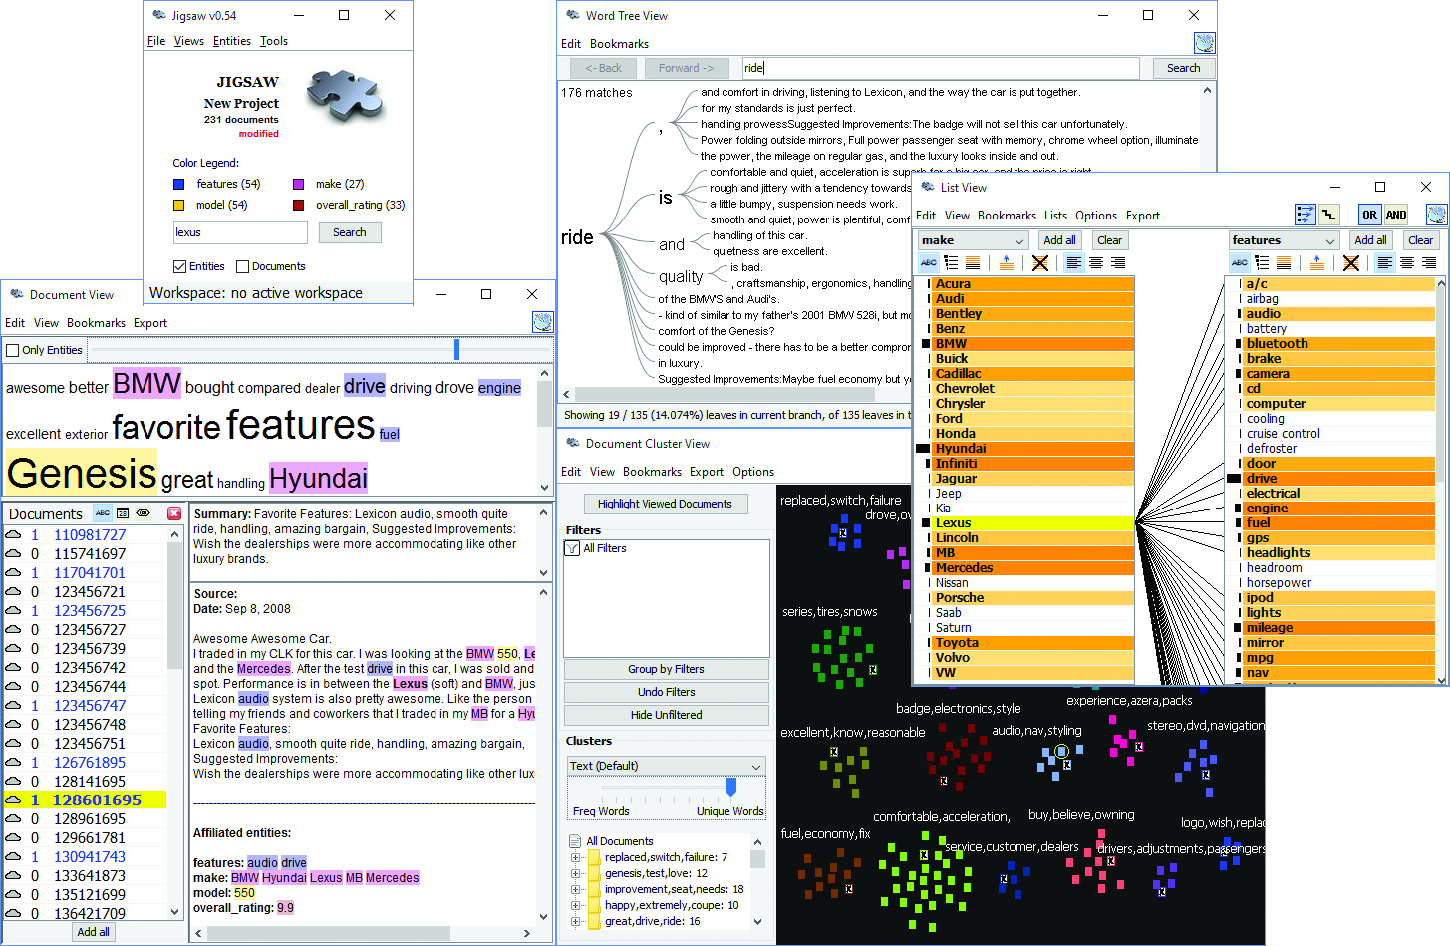
\includegraphics[width=0.9\linewidth]{ChapterViz/figures/fig9-11} 

}

\caption{Jigsaw used to explore a collection of car reviews}\label{fig:fig9-11}
\end{figure}

\section{Challenges}\label{sec:viz-4}

While information visualization is a powerful tool, there are many
obstacles to its effective use. We note here four areas of particular
concern: scalability, evaluation, visual impairment, and visual
literacy.

\subsection{Scalability}\label{sec:viz-4.1}

Most visualizations handle relatively small data sets (between a
thousand and a hundred thousand, sometimes up to millions, depending on
the technique) but scaling visualizations from millions to billions of
records does require careful coordination of analytic algorithms to
filter data or perform rapid aggregation, effective visual summary
designs, and rapid refreshing of displays (Shneiderman
\protect\hyperlink{ref-shneiderman2008extreme}{2008}). The visual
information seeking mantra, ``Overview first, zoom and filter, then
details on demand,'' remains useful with data at scale. To accommodate a
billion records, aggregate markers (which may represent thousands of
records) and density plots are useful (Dunne and Shneiderman
\protect\hyperlink{ref-dunne2013motif}{2013}). In some cases the large
volume of data can be aggregated meaningfully into a small number of
pixels. One example is Google Maps and its visualization of road
conditions. A quick glance at the map allows drivers to use a highly
aggregated summary of the speed of a large number of vehicles and only a
few red pixels are enough to decide when to get on the road.

While millions of graphic elements may be represented on large screens
(Fekete and Plaisant
\protect\hyperlink{ref-fekete2002interactive}{2002}), perception issues
need to be taken into consideration (Yost, Haciahmetoglu, and North
\protect\hyperlink{ref-yost2007beyond}{2007}). Extraction and filtering
may be necessary before even attempting to visualize individual records
(Wongsuphasawat and Lin
\protect\hyperlink{ref-wongsuphasawat2014using}{2014}). Preserving
interactive rates in querying big data sources is a challenge, with a
variety of methods proposed, such as approximations (Fisher et al.
\protect\hyperlink{ref-fisher2012trust}{2012}) and compact caching of
aggregated query results (Lins, Klosowski, and Scheidegger
\protect\hyperlink{ref-lins2013nanocubes}{2013}). Progressive loading
and processing will help users review the results as they appear and
steer the lengthy data processing (Glueck, Khan, and Wigdor
\protect\hyperlink{ref-glueck2014dive}{2014}; Fekete
\protect\hyperlink{ref-fekete2015progressivis}{2015}). Systems are
starting to emerge, and strategies to cope with volume and variety of
patterns are being described (Shneiderman and Plaisant
\protect\hyperlink{ref-shneiderman2015sharpening}{2015}).

\subsection{Evaluation}\label{sec:viz-4.2}

Human-centric evaluation of visualization techniques can generate
qualitative and quantitative assessments of their potential quality,
with early studies focusing on the effectiveness of basic visual
variables (MacKinlay
\protect\hyperlink{ref-mackinlay1986automating}{1986}). To this day,
user studies remain the workhorse of evaluation. In laboratory settings,
experiments can demonstrate faster task completion, reduced error rates,
or increased user satisfaction. These studies are helpful for comparing
visual and interaction designs. For example, studies are reporting on
the effects of latency on interaction and understanding (Liu and Heer
\protect\hyperlink{ref-liu2014effects}{2014}), and often reveal that
different visualizations perform better for different tasks (Saket et
al. \protect\hyperlink{ref-saket2014node}{2014}; Plaisant, Grosjean, and
Bederson \protect\hyperlink{ref-plaisant2002spacetree}{2002}).
Evaluations may also aim to measure and study the amount and value of
the insights revealed by the use of exploratory visualization tools
(Saraiya, North, and Duca
\protect\hyperlink{ref-saraiya2005insight}{2005}). Diagnostic usability
evaluation remains a cornerstone of user-centered design. Usability
studies can be conducted at various stages of the development process to
verify that users are able to complete benchmark tasks with adequate
speed and accuracy. Comparisons with the technology previously used by
target users may also be possible to verify improvements. Metrics need
to address the learnability and utility of the system, in addition to
performance and user satisfaction (Lam et al.
\protect\hyperlink{ref-lam2012empirical}{2012}). Usage data logging,
user interviews, and surveys can also help identification of potential
improvements in visualization and interaction design.

\subsection{Visual impairment}\label{sec:viz-4.3}

Color impairment is a common condition that needs to be taken into
consideration (Olson and Brewer
\protect\hyperlink{ref-olson1997evaluation}{1997}). For example, red and
green are appealing for their intuitive mapping to positive or negative
outcomes (also depending on cultural associations); however, users with
red--green color blindness, one of the most common forms, would not be
able to differentiate such scales clearly. To assess and assist visual
design under different color deficiencies, color simulation tools can be
used (see additional resources). The impact of color impairment can be
mitigated by careful selection of limited color schemes, using double
encoding when appropriate (i.e., using symbols that vary by both shape
and color), and allowing users to change or customize color palettes. To
accommodate users with low vision, adjustable size and zoom settings can
be useful. Users with severe visual impairments may require alternative
accessibility-first interface and interaction designs.

\subsection{Visual literacy}\label{sec:viz-4.4}

While the number of people using visualization continues to grow, not
everyone is able to accurately interpret graphs and charts. When
designing a visualization for a population of users who are expected to
make sense of the data without training, it is important to adequately
estimate the level of visual literacy of those users. Even simple
scatterplots can be overwhelming for some users. Recent work has
proposed new methods for assessing visual literacy (Boy et al.
\protect\hyperlink{ref-boy2014principled}{2014}), but user testing with
representative users in the early stages of design and development will
remain necessary to verify that adequate designs are being used.
Training is likely to be needed to help analysts get started when using
visual analytics tools. Recorded video demonstrations and online support
for question answering are helpful to bring users from novice to expert
levels.

\section{Summary}\label{sec:viz-5}

The use of information visualization is spreading widely, with a growing
number of commercial products and additions to statistical packages now
available. Careful user testing should be conducted to verify that
visual data presentations go beyond the desire for eye-candy in
visualization, and to implement designs that have demonstrated benefits
for realistic tasks. Visualization is becoming increasingly used by the
general public and attention should be given to the goal of universal
usability so the widest range of users can access and benefit from new
approaches to data presentation and interactive analysis.

\hypertarget{sec:viz-6}{\section{Resources}\label{sec:viz-6}}

We have referred to various textbooks throughout this chapter. Tufte's
books remain the classics, as inspiring to read as they are instructive
(Tufte \protect\hyperlink{ref-edward2001visual}{2001}; Tufte
\protect\hyperlink{ref-edward2006beauty}{2006}). We also recommend Few's
books on information visualization (Few
\protect\hyperlink{ref-few2009now}{2009}) and information dashboard
design (Few \protect\hyperlink{ref-few2013information}{2013}). See also
the book's website for further readings.

Given the wide variety of goals, tasks, and use cases of visualization,
many different data visualization tools have been developed that address
different needs and appeal to different skill levels. In this chapter we
can only point to a few examples to get started. To generate a wide
range of visualizations and dashboards, and to quickly share them
online, Tableau and Tableau Public provide a flexible visualization
design platform. If a custom design is required and programmers are
available, d3 is the de facto low-level library of choice for many
web-based visualizations, with its native integration to web standards
and flexible ways to convert and manipulate data into visual objects as
a JavaScript library. There exist other JavaScript web libraries that
offer chart templates (such as Highcharts), or web services that can be
used to create a range of charts from given (small) data sets, such as
Raw or DataWrapper. To clean, transform, merge, and restructure data
sources so that they can be visualized appropriately, tools like
Trifacta and Alteryx can be used to create pipelines for data wrangling.
For statistical analysis and batch-processing data, programming
environments such as R or libraries for languages such as Python (for
example, the Python Plotly library) can be used.

An extended list of visualization tools and books are available at
\url{https://gallery.keshif.me/VisTools} and
\url{https://gallery.keshif.me/VisBooks}.

The \emph{Dataset Exploration and Visualization} workbook of Chapter
\protect\hyperlink{chap:workbooks}{Workbooks} uses \texttt{matplotlib}
and \texttt{seaborn} for creating basic visualizations with
Python.\footnote{See \url{https://workbooks.coleridgeinitiative.org}.}

\hypertarget{chap:ml}{\chapter{Machine Learning}\label{chap:ml}}

\textbf{Rayid Ghani and Malte Schierholz}

This chapter introduces you to the use of machine learning in tackling
social science and public policy problems. We cover the end-to-end
machine learning process and focus on clustering and classification
methods. After reading this chapter, you should have an overview of the
components of a machine learning pipeline and methods, and know how to
use those in solving social science problems. We have written this
chapter to give an intuitive explanation for the methods and to provide
a framework and practical tips on how to use them in practice.

\section{Introduction}\label{introduction-2}

You have probably heard of ``machine learning'' but are not sure exactly
what it is, how it differs from traditional statistics, and what you, as
social scientists, can do with it. In this chapter, we will demystify
machine learning, draw connections to what you already know from
statistics and data analysis, and go deeper into some of the novel
concepts and methods that have been developed in this field. Although
the field originates from computer science, it has been influenced quite
heavily by math and statistics in the past 15--20 years. As you will
see, many of the concepts you will learn are not entirely new, but are
simply called something else. For example, you already are familiar with
logistic regression (a classification method that falls under the
supervised learning framework in machine learning) and cluster analysis
(a form of unsupervised learning). You will also learn about new methods
that are more exclusively used in machine learning, such as random
forests, support vector machines, and neural networks. We will keep
formalisms to a minimum and focus on getting the intuition across, as
well as providing practical tips. Our hope is this chapter will make you
comfortable and familiar with machine learning vocabulary, concepts, and
processes, and allows you to further explore and use these methods and
tools in your own research and practice.

\section{What is machine learning?}\label{what-is-machine-learning}

When humans improve their skills with experience, they are said to
learn. Is it also possible to program computers to do the same? Arthur
Samuel, who coined the term \emph{machine learning} in 1959 (Samuel
\protect\hyperlink{ref-samuel1959some}{1959}), was a pioneer in this
area, programming a computer to play checkers. The computer played
against itself and human opponents, improving its performance with every
game. Eventually, after sufficient \emph{training} (and experience), the
computer became a better player than the human programmer. Today,
machine learning has grown significantly beyond learning to play
checkers. Machine learning systems have learned to drive (and park)
autonomous cars, are embedded inside robots, can recommend books,
products, and movies we are (sometimes) interested in, identify drugs,
proteins, and genes that should be investigated further to cure
diseases, detect cancer and other pathologies in x-rays and other types
of medical imaging, help us understand how the human brain learns
language, help identify which voters are persuadable in elections,
detect which students are likely to need extra support to graduate high
school on time, and help solve many more problems. Over the past 20
years, machine learning has become an interdisciplinary field spanning
computer science, artificial intelligence, databases, and statistics. At
its core, machine learning seeks to design computer systems that improve
over time with more experience. In one of the earlier books on machine
learning, Tom Mitchell gives a more operational definition, stating
that: ``A computer program is said to learn from experience \(E\) with
respect to some class of tasks \(T\) and performance measure \(P\), if
its performance at tasks in \(T\), as measured by \(P\), improves with
experience \(E\)'' (Mitchell
\protect\hyperlink{ref-mitchell1997machine}{1997}). We like this
definition because it is task-focused and allows us to think of machine
learning as a tool used inside a larger system to improve outcomes that
we care about.

\begin{center}\rule{0.5\linewidth}{\linethickness}\end{center}

\textbf{Box: Commercial machine learning examples}

\begin{itemize}
\item
  \textbf{Speech recognition}: Speech recognition software uses machine
  learning algorithms that are built on large amounts of initial
  training data. Machine learning allows these systems to be tuned and
  adapt to individual variations in speaking as well as across different
  domains.
\item
  \textbf{Autonomous cars}: The ongoing development of self-driving cars
  applies techniques from machine learning. An onboard computer
  continuously analyzes the incoming video and sensor streams in order
  to monitor the surroundings. Incoming data are matched with annotated
  images to recognize objects like pedestrians, traffic lights, and
  potholes. In order to assess the different objects, huge training data
  sets are required where similar objects already have been identified.
  This allows the autonomous car to decide on which actions to take
  next.
\item
  \textbf{Fraud detection}: Many public and private organizations face
  the problem of fraud and abuse. Machine learning systems are widely
  used to take historical cases of fraud and flag fraudulent
  transactions as they take place. These systems have the benefit of
  being adaptive, and improving with more data over time.
\item
  \textbf{Personalized ads}: Many online stores have personalized
  recommendations promoting possible products of interest. Based on
  individual shopping history and what other similar users bought in the
  past, the website predicts products a user may like and tailors
  recommendations. Netflix and Amazon are two examples of companies
  whose recommendation software predicts how a customer would rate a
  certain movie or product and then suggests items with the highest
  predicted ratings. Of course there are some caveats here, since they
  then adjust the recommendations to maximize profits.
\item
  \textbf{Face recognition}: Surveillance systems, social networking
  platforms, and imaging software all use face detection and face
  recognition to first detect faces in images (or video) and then tag
  them with individuals for various tasks. These systems are trained by
  giving examples of faces to a machine learning system which then
  learns to detect new faces, and tag known individuals. The bias and
  fairness chapter will highlight some concerns with these types of
  systems.
\end{itemize}

\begin{center}\rule{0.5\linewidth}{\linethickness}\end{center}

\begin{center}\rule{0.5\linewidth}{\linethickness}\end{center}

\textbf{Box: Social Science machine learning examples}

Potash et al (\protect\hyperlink{ref-Potash2015}{2015}) worked with the
Chicago Department of Public Health and used random forests (a machine
learning classification method) to predict which children are at risk of
lead poisoning. This early warning system was then used to prioritize
lead hazard inspections to detect and remediate lead hazards before they
had an adverse effect on the child.

Carton et al (\protect\hyperlink{ref-Carton2016}{2016}) used a
collection of machine learning methods to identify police officers at
risk of adverse behavior, such as unjustified use of force or
unjustified shootings or sustained complaints, to prioritize preventive
interventions such as training and counseling.

Athey and Wager (\protect\hyperlink{ref-athey2019}{2019}) use a
modification of random forests to estimate heterogeneous treatment
effects using a data set from The National Study of Learning Mindsets to
evaluate the impact of interventions to improve student achievement.

Voigt et al (\protect\hyperlink{ref-Voigt2017}{2017}) uses machine
learning methods to analyze footage from body-worn cameras and
understand the respectfulness of police officer language toward white
and black community members during routine traffic stops.

\begin{center}\rule{0.5\linewidth}{\linethickness}\end{center}

Machine learning grew from the need for systems that were adaptive,
scalable, and cost-effective to build and maintain. A lot of tasks now
being done using machine learning used to be done by rule-based systems,
where experts would spend considerable time and effort developing and
maintaining the rules. The problem with those systems was that they were
rigid, not adaptive, hard to scale, and expensive to maintain. Machine
learning systems started becoming popular because they could improve the
system along all of these dimensions\footnote{See Chapter
  \protect\hyperlink{chap:link}{Record Linkage}.}. Box
\protect\hyperlink{box:ml1}{Applications} mentions several examples
where machine learning is being used in commercial applications today.
Social scientists are uniquely placed today to take advantage of the
same advances in machine learning by having better methods to solve
several key problems they are tackling. Box
\protect\hyperlink{box:ml2}{Social Science} describes a few social
science and policy problems that are being tackled using machine
learning today.\footnote{If you have examples from your own research
  using the methods we describe in this chapter, please submit a link to
  the paper (and/or code) here:
  \url{https://textbook.coleridgeinitiative.org/submitexamples}}

This chapter is not an exhaustive introduction to machine learning.
There are many books that have done an excellent job of that (Flach
\protect\hyperlink{ref-Flach}{2012}; Hastie, Tibshirani, and Friedman
\protect\hyperlink{ref-HastieTibshirani}{2001}; Mitchell
\protect\hyperlink{ref-mitchell1997machine}{1997}). Instead, we present
a short and accessible introduction to machine learning for social
scientists, give an overview of the overall machine learning process,
provide an intuitive introduction to machine learning methods, give some
practical tips that will be helpful in using these methods, and leave a
lot of the statistical theory to machine learning textbooks. As you read
more about machine learning in the research literature or the media, you
will encounter names of other fields that are related (and practically
the same for most social science audiences), such as statistical
learning, data mining, and pattern recognition.

\section{Types of analysis}\label{types-of-analysis}

A lot of the data analysis tasks that social scientists do can be broken
down into four types:

\begin{itemize}
\item
  \textbf{Description}: The goal is to describe patterns or groupings in
  historical data. You're already familiar with descriptive statistics
  and exploratory data analysis methods, and we will cover more advanced
  versions of those later in this chapter under Unsupervised Learning.
\item
  \textbf{Detection}: The goal here is not to necessarily understand
  historical behavior but to detect new or emerging anomalies, events,
  or patterns as they happen. A typical example is early outbreak
  detection for infectious diseases in order to inform public health
  officials.
\item
  \textbf{Prediction}: The goal here is to use the same historical data
  as the description and detection methods, but use it to predict events
  and behaviors in the future.
\item
  \textbf{Behavior Change (or Causal Inference)}: The goal here is to
  understand the causal relationships in the data in order to influence
  the outcomes we care about.
\end{itemize}

In this chapter, we will mostly focus on Description and Prediction
methods but there is a lot of work going in developing and using machine
learning methods for detection as well as for behavior change and causal
inference.

\section{The Machine Learning
process}\label{the-machine-learning-process}

When solving problems using machine learning methods, it is important to
think of the larger data-driven problem-solving process of which these
methods are a small part\footnote{See Chapter
  \protect\hyperlink{chap:link}{Record Linkage}.}. A typical machine
learning problem requires researchers and practitioners to take the
following steps:

\begin{enumerate}
\def\labelenumi{\arabic{enumi}.}
\item
  \textbf{Understand the problem and goal}: This sounds obvious but is
  often nontrivial. Problems typically start as vague descriptions of a
  goal---improving health outcomes, increasing graduation rates,
  understanding the effect of a variable \(X\) on an outcome \(Y\), etc.
  It is really important to work with people who understand the domain
  being studied to discuss and define the problem more concretely. What
  is the analytical formulation of the metric that you are trying to
  improve? The Data Science Project Scoping Guide\footnote{\url{http://www.datasciencepublicpolicy.org/home/resources/data-science-project-scoping-guide/}}
  is a good place to start when doing problem scoping for social science
  or policy problems
\item
  \textbf{Formulate it as a machine learning problem}: Is it a
  classification problem or a regression problem? Is the goal to build a
  model that generates a ranked list prioritized by risk of an outcome,
  or is it to detect anomalies as new data come in? Knowing what kinds
  of tasks machine learning can solve will allow you to map the problem
  you are working on to one or more machine learning settings and give
  you access to a suite of methods appropriate for that task.
\item
  \textbf{Data exploration and preparation}: Next, you need to carefully
  explore the data you have. What additional data do you need or have
  access to? What variable will you use to match records for integrating
  different data sources? What variables exist in the data set? Are they
  continuous or categorical? What about missing values? Can you use the
  variables in their original form or do you need to alter them in some
  way?
\item
  \textbf{Feature engineering}: In machine learning language, what you
  might know as independent variables or predictors or factors or
  covariates are called ``features.'' Creating good features is probably
  the most important step in the machine learning process. This involves
  doing transformations, creating interaction terms, or aggregating over
  data points or over time and space.
\item
  \textbf{Modeling}: Having formulated the problem and created your
  features, you now have a suite of methods to choose from. It would be
  great if there were a single method that always worked best for a
  specific type of problem, but that would make things too easy. Each
  method makes a difference assumption about the structure and
  distribution of the data and with large amounts of high-dimensional
  data\footnote{Dimensionality of the data often refers to how many
    variables we have in the data.}, it is difficult to know apriori
  which assumption will best match the data we have. Typically, in
  machine learning, you take a collection of methods and try them out to
  empirically validate which one works the best for your problem. This
  process not only helps you select the best method for your problem but
  also helps you understand the structure of your data. We will give an
  overview of leading methods that are being used today in this chapter.
\item
  \textbf{Model Interpretation}: Once we have built the machine learning
  models, we also want to understand what they are, which predictors
  they found important, and how much, what types of entities they
  flagged as high risk (and why), where they made errors, etc. All of
  these fall under the model interpretation, interpretability,
  explainability umbrella which is an active area of research right now
  in machine learning.
\item
  \textbf{Model Selection}: As you build a large number of possible
  models, you need a way to select the model that is the ``best''. This
  part of the chapter will cover methodology to first test the models on
  historical data as well as discuss a variety of evaluation metrics.
  While this chapter will focus mostly on traditionally used metrics,
  Chapter \protect\hyperlink{chap:bias}{Bias and Fairness} will expand
  on this using bias and fairness related metrics. It is important to
  note that sometimes the machine learning literature will call this
  step the ``validation'' step using historical data, but we want to
  distinguish it here from validation, which is the next step.
\item
  \textbf{Model Validation}: The next step, after model selection (using
  historical data) is validation. Validate on new data, as well as
  designing and running field trials or experiments.
\item
  \textbf{Deployment and Monitoring}: Once you have selected the best
  model and validated it using historical data as well as a field trial,
  you are ready to put the model into practice. You still have to keep
  in mind that new data will be coming in, the world will be changing,
  and the model might also (need to) change over time. We will not cover
  too much of those aspects in this chapter, but they are important to
  keep in mind when putting the machine learning work in to practice.
\end{enumerate}

Although each step in this process is critical, a thorough description
of each is out of scope. This chapter will focus on models, terms, and
techniques that form the core of machine learning.

\section{Problem formulation: Mapping a problem to machine learning
methods}\label{problem-formulation-mapping-a-problem-to-machine-learning-methods}

When working on a new problem, one of the first things we need to do is
to map it to a class of machine learning methods. In general, the
problems we will tackle, including the examples above, can be grouped
into two major categories:

\begin{enumerate}
\def\labelenumi{\arabic{enumi}.}
\item
  \textbf{Supervised learning}: These are problems where there exists a
  target variable (continuous or discrete) that we want to predict or
  classify data into. Classification, prediction, and regression all
  fall into this category. More formally, supervised learning methods
  predict a value \(Y\) given input(s) \(X\) by learning (or estimating
  or fitting or training) a function \(F\), where \(F(X) = Y\). Here,
  \(X\) is the set of variables (known as \emph{features} in machine
  learning, or in other fields as \emph{predictors}) provided as input
  and \(Y\) is the target/dependent variable or a \emph{label} (as it is
  known in machine learning).

  The goal of supervised learning methods is to search for that function
  \(F\) that best estimates or predicts \(Y\). When the output \(Y\) is
  categorical, this is known as \emph{classification}. When \(Y\) is a
  continuous value, this is called \emph{regression}. Sound familiar?

  One key distinction in machine learning is that the goal is not just
  to find the best function \(F\) that can estimate or predict \(Y\) for
  observed outcomes (known \(Y\)s) but to find one that best generalizes
  to new, unseen data, often in the future. This distinction makes
  methods more focused on generalization and less on just fitting the
  data we have as best as we can. It is important to note that you do
  that implicitly when performing regression by not adding more and more
  higher-order terms to get better fit statistics. By getting better fit
  statistics, we \emph{overfit} to the data and the performance on new
  (unseen) data often goes down. Methods like the lasso (Tibshirani
  \protect\hyperlink{ref-tibshirani1996regression}{1996}) penalize the
  model for having too many terms by performing what is known as
  \emph{regularization}\footnote{In statistical terms, regularization is
    an attempt to avoid overfitting the model.}.
\item
  \textbf{Unsupervised learning}: These are problems where there does
  not exist a target variable that we want to predict but we want to
  understand ``natural'' groupings or patterns in the data. Clustering
  is the most common example of this type of analysis where you are
  given \(X\) and want to group similar \(X\)s together. You may have
  heard of ``segmentation'' that's used in the marketing world to group
  similar customers together using clustering techniques. Principal
  components analysis (PCA) and related methods also fall into the
  unsupervised learning category.
\end{enumerate}

In between the two extremes of supervised and unsupervised learning,
there is a spectrum of methods that have different levels of supervision
involved (Figure \ref{fig:spectrum}). Supervision in this case is the
presence of target variables (known in machine learning as
\emph{labels}). In unsupervised learning, none of the data points have
labels. In supervised learning, all data points have labels. In between,
either the percentage of examples with labels can vary or the types of
labels can vary. We do not cover the weakly supervised and
semi-supervised methods much in this chapter, but this is an active area
of research in machine learning. Zhu
(\protect\hyperlink{ref-zhu2005semi}{2008}) provides more details.

\begin{figure}

{\centering 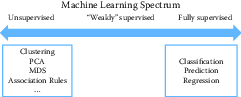
\includegraphics[width=0.7\linewidth]{ChapterML/figures/spectrum} 

}

\caption{Spectrum of machine learning methods from unsupervised to supervised learning}\label{fig:spectrum}
\end{figure}

\subsection{Features}\label{features}

Before we get to models and methods, we need to turn our raw data into
``features''. In social science, they are not called features but
instead are known as variables or predictors (or covariates if you're
doing regression).\footnote{Good features are what makes machine
  learning systems effective.} Feature generation (or engineering, as it
is often called) is where a large chunk of the time is spent in the
machine learning process. This is also the phase where previous research
and learnings from the domain being tackled can be incorporated into the
machine learning process. As social science researchers or
practitioners, you have spent a lot of time constructing features, using
transformations, dummy variables, and interaction terms. All of that is
still required and critical in the machine learning framework. One
difference you will need to get comfortable with is that instead of
carefully selecting a few predictors, machine learning systems tend to
encourage the creation of \emph{lots} of features and then empirically
use holdout data to perform regularization and model selection. It is
common to have models that are trained on thousands of features. Of
course, it is important to keep in mind that increasing the number of
features requires you to have enough data so that you're not
overfitting. Commonly used approaches to create features include:

\begin{itemize}
\item
  \textbf{Transformations}, such as log, square, and square root.
\item
  \textbf{Dummy (binary) variables}: This is often done by taking
  categorical variables (such as city) and creating a binary variable
  for each value (one variable for each city in the data). These are
  also called indicator variables.
\item
  \textbf{Discretization}: Several methods require features to be
  discrete instead of continuous. Several approaches exist to convert
  continuous variables into discrete ones, the most common of which is
  equal-width binning.
\item
  \textbf{Aggregation}: Aggregate features often constitute the majority
  of features for a given problem. These aggregations use different
  aggregation functions (count, min, max, average, standard deviation,
  etc.), often over varying windows of time and space. For example,
  given urban data, we would want to calculate the number (and min, max,
  mean, variance) of crimes within an \(m\)-mile radius of an address in
  the past \(t\) months for varying values of \(m\) and \(t\), and then
  to use all of them as features in a classification problem.
  Spatiotemporal aggregation features are going to be extremely
  important as you build machine learning models.
\end{itemize}

In general, it is a good idea to have the complexity in features and use
a simple model, rather than using more complex models with simple
features. Keeping the model simple makes it faster to train and easier
to understand and explain.

\section{Methods}\label{methods}

We will start by describing unsupervised learning methods and then go on
to supervised learning methods. We focus here on the intuition behind
the methods and the algorithm, as well as some practical tips, rather
than on the statistical theory that underlies the methods. We encourage
readers to refer to machine learning books listed in Section
\protect\hyperlink{ml:res}{Resources}. Box
\protect\hyperlink{box:ml3}{Vocabulary} gives brief definitions of
several terms we will use in this section.

\begin{center}\rule{0.5\linewidth}{\linethickness}\end{center}

\textbf{Box 7.3: Machine learning vocabulary}

\begin{itemize}
\item
  \textbf{Learning}: In machine learning, you will notice the term
  \emph{learning} that will be used in the context of ``learning'' a
  model. This is what you probably know as \emph{fitting} or
  \emph{estimating} a function, or \emph{training} or \emph{building} a
  model. These terms are all synonyms and are used interchangeably in
  the machine learning literature.
\item
  \textbf{Examples}: These are data points, rows, observations, or
  instances.
\item
  \textbf{Features}: These are independent variables, attributes,
  predictor variables, and explanatory variables.
\item
  \textbf{Labels}: These include the response variable, dependent
  variable, target variable, or outcomes.
\item
  \textbf{Underfitting}: This happens when a model is too simple and
  does not capture the structure of the data well enough.
\item
  \textbf{Overfitting}: This happens when a model is possibly too
  complex and models the noise in the data, which can result in poor
  generalization performance. Using in-sample measures to do model
  selection can result in that.
\item
  \textbf{Regularization}: This is a general method to avoid overfitting
  by applying additional constraints to the model that is learned. For
  example, in building logistic regression models, a common approach is
  to make sure the model weights (coefficients) are, on average, small
  in magnitude. Two common regularizations are \(L_1\) regularization
  (used by the lasso), which has a penalty term that encourages the sum
  of the absolute values of the parameters to be small; and \(L_2\)
  regularization, which encourages the sum of the squares of the
  parameters to be small.
\end{itemize}

\begin{center}\rule{0.5\linewidth}{\linethickness}\end{center}

\subsection{Unsupervised learning
methods}\label{unsupervised-learning-methods}

As mentioned earlier, unsupervised learning methods are used when we do
not have a target variable to estimate or predict but want to understand
clusters, groups, or patterns in the data. These methods are often used
for data exploration, as in the following examples:

\begin{enumerate}
\def\labelenumi{\arabic{enumi}.}
\item
  When faced with a large corpus of text data---for example, email
  records, congressional bills, speeches, or open-ended free-text survey
  responses---unsupervised learning methods are often used to understand
  and get a handle on the patterns in our data.
\item
  Given a data set about students and their behavior over time (academic
  performance, grades, test scores, attendance, etc.), one might want to
  understand typical behaviors as well as trajectories of these
  behaviors over time. Unsupervised learning methods (clustering) can be
  applied to these data to get student ``segments'' with similar
  behavior.
\item
  Given a data set about publications or patents in different fields, we
  can use unsupervised learning methods (association rules) to figure
  out which disciplines have the most collaboration and which fields
  have researchers who tend to publish across different fields.
\item
  Given a set of people who are at high risk of recidivism, clustering
  can be used to understand different groups of people within the high
  risk set, to determine intervention programs that may need to be
  created.
\end{enumerate}

\textbf{Clustering}

Clustering is the most common unsupervised learning technique and is
used to group data points together that are similar to each other. The
goal of clustering methods is to produce with high intra-cluster
(within) similarity and low inter-cluster (between) similarity.

Clustering algorithms typically require a distance (or similarity)
metric\footnote{Distance metrics are mathematical formulas to calculate
  the distance between two objects. For example, \emph{Manhattan
  distance} is the distance a car would drive from one place to another
  place in a grid-based street system, whereas \emph{Euclidean distance}
  (in two-dimensional space) is the ``straight-line'' distance between
  two points.} to generate clusters. They take a data set and a distance
metric (and sometimes additional parameters), and they generate clusters
based on that distance metric. The most common distance metric used is
Euclidean distance, but other commonly used metrics are Manhattan,
Minkowski, Chebyshev, cosine, Hamming, Pearson, and Mahalanobis. Often,
domain-specific similarity metrics can be designed for use in specific
problems. For example, when performing the record linkage tasks
discussed in Chapter \protect\hyperlink{chap:link}{Record Linkage}, you
can design a similarity metric that compares two first names and assigns
them a high similarity (low distance) if they both map to the same
canonical name, so that, for example, Sammy and Sam map to Samuel.

Most clustering algorithms also require the user to specify the number
of clusters (or some other parameter that indirectly determines the
number of clusters) in advance as a parameter. This is often difficult
to do a priori and typically makes clustering an iterative and
interactive task. Another aspect of clustering that makes it interactive
is often the difficulty in automatically evaluating the quality of the
clusters. While various analytical clustering metrics have been
developed, the best clustering is task-dependent and thus must be
evaluated by the user. There may be different clusterings that can be
generated with the same data. You can imagine clustering similar news
stories based on the topic content, based on the writing style or based
on sentiment. The right set of clusters depends on the user and the task
they have. Clustering is therefore typically used for exploring the
data, generating clusters, exploring the clusters, and then rerunning
the clustering method with different parameters or modifying the
clusters (by splitting or merging the previous set of clusters).
Interpreting a cluster can be nontrivial: you can look at the centroid
of a cluster, look at frequency distributions of different features (and
compare them to the prior distribution of each feature), or you can
build a decision tree (a supervised learning method we will cover later
in this chapter) where the target variable is the cluster ID that can
describe the cluster using the features in your data. A good example of
a tool that allows interactive clustering from text data is Ontogen
(Fortuna, Grobelnik, and Mladenic
\protect\hyperlink{ref-Ontogen}{2007}).

\textbf{\(k\)-means clustering}

The most commonly used clustering algorithm is called \(k\)-means, where
\(k\) defines the number of clusters. The algorithm works as follows:

\begin{enumerate}
\def\labelenumi{\arabic{enumi}.}
\item
  Select \(k\) (the number of clusters you want to generate).
\item
  Initialize by selecting \(k\) points as centroids of the \(k\)
  clusters. This is typically done by selecting \(k\) points uniformly
  at random.
\item
  Assign each point a cluster according to the nearest centroid.
\item
  Recalculate cluster centroids based on the assignment in (3) as the
  mean of all data points belonging to that cluster.
\item
  Repeat (3) and (4) until convergence.
\end{enumerate}

The algorithm stops when the assignments do not change from one
iteration to the next (Figure \ref{fig:kmeans}). The final set of
clusters, however, depend on the starting points. If they are
initialized differently, it is possible that different clusters are
obtained. One common practical trick is to run \(k\)-means several
times, each with different (random) starting points. The \(k\)-means
algorithm is fast, simple, and easy to use, and is often a good first
clustering algorithm to try and see if it fits your needs. When the data
are of the form where the mean of the data points cannot be computed, a
related method called \(K\)-medoids can be used (Park and Jun
\protect\hyperlink{ref-park2009simple}{2009}).

\begin{figure}

{\centering 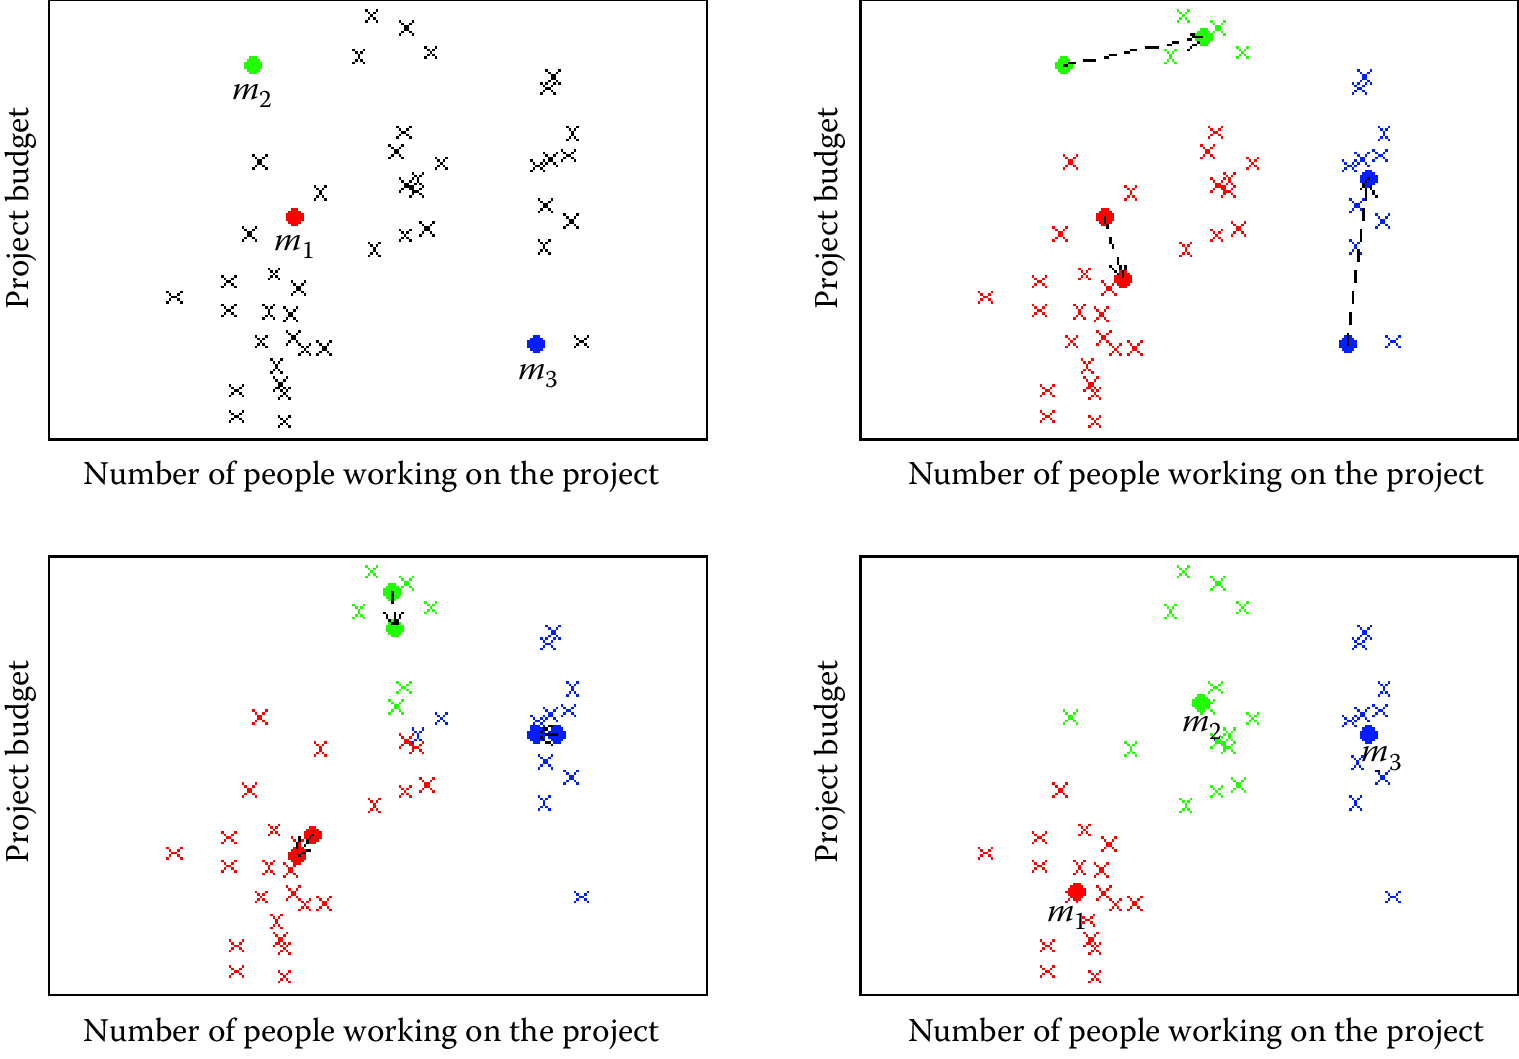
\includegraphics[width=0.7\linewidth]{ChapterML/figures/kmeans} 

}

\caption{Example of $k$-means clustering with $k = 3$. The upper left panel shows the distribution of the data and the three starting points $m_1$, $m_2$, $m_3$ placed at random. On the upper right we see what happens in the first iteration. The cluster means move to more central positions in their respective clusters. The lower left panel shows the second iteration. After six iterations the cluster means have converged to their final destinations and the result is shown in the lower right panel}\label{fig:kmeans}
\end{figure}

\textbf{Expectation-maximization (EM) clustering}

You may be familiar with the EM algorithm in the context of imputing
missing data. EM is a general approach to maximum likelihood in the
presence of incomplete data. However, it is also used as a clustering
method where the missing data are the clusters a data point belongs to.
Unlike \(k\)-means, where each data point gets assigned to only one
cluster, EM does a soft assignment where each data point gets a
probabilistic assignment to various clusters. The EM algorithm iterates
until the estimates converge to some (locally) optimal solution.

The EM algorithm is fairly good at dealing with outliers as well as
high-dimensional data, compared to \(k\)-means. It also has a few
limitations. First, it does not work well with a large number of
clusters or when a cluster contains few examples. Also, when the value
of \(k\) is larger than the number of actual clusters in the data, EM
may not give reasonable results.

\textbf{Mean shift clustering}

Mean shift clustering works by finding dense regions in the data by
defining a window around each data point and computing the mean of the
data points in the window. Then it shifts the center of the window to
the mean and repeats the algorithm till it converges. After each
iteration, we can consider that the window shifts to a denser region of
the data set. The algorithm proceeds as follows:

\begin{enumerate}
\def\labelenumi{\arabic{enumi}.}
\item
  Fix a window around each data point (based on the bandwidth parameter
  that defines the size of the window).
\item
  Compute the mean of data within the window.
\item
  Shift the window to the mean and repeat till convergence.
\end{enumerate}

Mean shift needs a bandwidth parameter \(h\) to be tuned, which
influences the convergence rate and the number of clusters. A large
\(h\) might result in merging distinct clusters. A small \(h\) might
result in too many clusters. Mean shift might not work well in higher
dimensions since the number of local maxima is pretty high and it might
converge to a local optimum quickly.

One of the most important differences between mean shift and \(k\)-means
is that \(k\)-means makes two broad assumptions: the number of clusters
is already known and the clusters are shaped spherically (or
elliptically). Mean shift does not assume anything about the number of
clusters (but the value of \(h\) indirectly determines that). Also, it
can handle arbitrarily shaped clusters.

The \(k\)-means algorithm is also sensitive to initializations, whereas
mean shift is fairly robust to initializations. Typically, mean shift is
run for each point, or sometimes points are selected uniformly randomly.
Similarly, \(k\)-means is sensitive to outliers, while mean shift is
less sensitive. On the other hand, the benefits of mean shift come at a
cost---speed. The \(k\)-means procedure is fast, whereas classic mean
shift is computationally slow but can be easily parallelized.

\textbf{Hierarchical clustering}

The clustering methods that we have seen so far, often termed
\emph{partitioning} methods, produce a flat set of clusters with no
hierarchy. Sometimes, we want to generate a hierarchy of clusters, and
methods that can do that are of two types:

\begin{enumerate}
\def\labelenumi{\arabic{enumi}.}
\item
  \textbf{Agglomerative (bottom-up)}: Start with each point as its own
  cluster and iteratively merge the closest clusters. The iterations
  stop either when the clusters are too far apart to be merged (based on
  a predefined distance criterion) or when there is a sufficient number
  of clusters (based on a predefined threshold).
\item
  \textbf{Divisive (top-down)}: Start with one cluster and create splits
  recursively.
\end{enumerate}

Typically, agglomerative clustering is used more often than divisive
clustering. One reason is that it is significantly faster, although both
of them are typically slower than direct partition methods such as
\(k\)-means and EM. Another disadvantage of these methods is that they
are \emph{greedy}, that is, a data point that is incorrectly assigned to
the ``wrong'' cluster in an earlier split or merge cannot be reassigned
again later on.

\textbf{Spectral clustering}

Figure \ref{fig:spectral} shows the clusters that \(k\)-means would
generate on the data set in the figure. It is obvious that the clusters
produced are not the clusters you would want, and that is one drawback
of methods such as \(k\)-means. Two points that are far away from each
other will be put in different clusters even if there are other data
points that create a ``path'' between them. Spectral clustering fixes
that problem by clustering data that are connected but not necessarily
(what is called) compact or clustered within convex boundaries. Spectral
clustering methods work by representing data as a graph (or network),
where data points are nodes in the graph and the edges (connections
between nodes) represent the similarity between the two data points.

\begin{figure}

{\centering 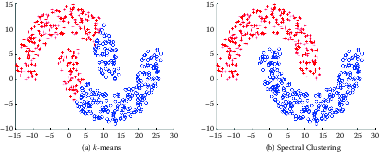
\includegraphics[width=0.7\linewidth]{ChapterML/figures/spectral} 

}

\caption{The same data set can produce drastically different clusters: (a) k-means; (b) spectral clustering}\label{fig:spectral}
\end{figure}

The algorithm works as follows:

\begin{enumerate}
\def\labelenumi{\arabic{enumi}.}
\item
  Compute a similarity matrix from the data. This involves determining a
  pairwise distance function (using one of the distance functions we
  described earlier).
\item
  With this matrix, we can now perform graph partitioning, where
  connected graph components are interpreted as clusters. The graph must
  be partitioned such that edges connecting different clusters have low
  weights and edges within the same cluster have high values.
\item
  We can now partition these data represented by the similarity matrix
  in a variety of ways. One common way is to use the normalized cuts
  method. Another way is to compute a graph Laplacian from the
  similarity matrix.
\item
  Compute the eigenvectors and eigenvalues of the Laplacian.
\item
  The \(k\) eigenvectors are used as proxy data for the original data
  set, and they are fed into \(k\)-means clustering to produce cluster
  assignments for each original data point.
\end{enumerate}

Spectral clustering is in general much better than \(k\)-means in
clustering performance but much slower to run in practice. For
large-scale problems, \(k\)-means is a preferred clustering algorithm to
run because of efficiency and speed.

\textbf{Principal components analysis}

Principal components analysis is another unsupervised method used for
finding patterns and structure in data. In contrast to clustering
methods, the output is not a set of clusters but a set of
\emph{principal components} that are linear combinations of the original
variables. PCA is typically used when you have a large number of
variables and you want a reduced number that you can analyze. This
approach is often called \emph{dimensionality reduction}. It generates
linearly uncorrelated dimensions that can be used to understand the
underlying structure of the data. In mathematical terms, given a set of
data on \(n\) dimensions, PCA aims to find a linear subspace of
dimension \(d\) lower than \(n\) such that the data points lie mainly on
this linear subspace.

PCA is related to several other methods you may already know about.
Multidimensional scaling, factor analysis, and independent component
analysis differ from PCA in the assumptions they make, but they are
often used for similar purposes of dimensionality reduction and
discovering the underlying structure in a data set.

\textbf{Association rules}

Association rules are a different type of analysis method and originate
from the data mining and database community, primarily focused on
finding frequent co-occurring associations among a collection of items.
This method is sometimes referred to as ``market basket analysis,''
since that was the original application area of association rules. The
goal is to find associations of items that occur together more often
than you would randomly expect. The classic example (probably a myth) is
``men who go to the store to buy diapers will also tend to buy beer at
the same time.'' This type of analysis would be performed by applying
association rules to a set of supermarket purchase data. For social
scientists, this method can be used on data that contains social
services that individuals have received in the past to determine what
types of services ``co-occur'' in people and proactively offer those
services to people in need.

Association rules take the form \(X_1, X_2, X_3 \Rightarrow Y\) with
support \(S\) and confidence \(C\), implying that when a transaction
contains items \(\{X_1, X_2, X_3\}\) \(C\)\% of the time, they also
contain item \(Y\) and there are at least \(S\)\% of transactions where
the antecedent is true. This is useful in cases where we want to find
patterns that are both \emph{frequent} and \emph{statistically
significant}, by specifying thresholds for support \(S\) and confidence
\(C\).

Support and confidence are useful metrics to generate rules but are
often not enough. Another important metric used to generate rules (or
reduce the number of spurious patterns generated) is \emph{lift}. Lift
is simply estimated by the ratio of the joint probability of two items,
\(x\) and \(y\), to the product of their individual probabilities:
\(P(x,y)/[P(x)P(y)]\). If the two items are statistically independent,
then \(P(x,y)=P(x)P(y)\), corresponding to a lift of \(1\). Note that
anti-correlation yields lift values less than 1, which is also an
interesting pattern, corresponding to mutually exclusive items that
rarely occur together.

Association rule algorithms work as follows: Given a set of transactions
(rows) and items for that transaction:

\begin{enumerate}
\def\labelenumi{\arabic{enumi}.}
\item
  Find all combinations of items in a set of transactions that occur
  with a specified minimum frequency. These combinations are called
  \emph{frequent itemsets}.
\item
  Generate association rules that express co-occurrence of items within
  frequent itemsets.
\end{enumerate}

For our purposes, association rule methods are an efficient way to take
a \emph{basket} of features (e.g., areas of publication of a researcher,
different organizations an individual has worked at in their career, all
the cities or neighborhoods someone may have lived in) and find
co-occurrence patterns. This may sound trivial, but as data sets and
number of features get larger, it becomes computationally expensive and
association rule mining algorithms provide a fast and efficient way of
doing it.

\subsection{Supervised learning}\label{sec:MLchapter:super}

We now turn to the problem of supervised learning, which typically
involves methods for classification, prediction, and regression. We will
mostly focus on classification methods in this chapter since many of the
regression methods in machine learning are fairly similar to methods
with which you are already familiar. Remember that classification means
predicting a discrete (or categorical) variable. Most of the
classification methods that we will cover can also be used for
Regression (predicting continuous outcomes).

In general, supervised learning methods take as input pairs of data
points \((X,Y)\) where \(X\) are the predictor variables (features) and
\(Y\) is the target variable (label). The supervised learning method
then uses these pairs as \emph{training data} and \emph{learns} a model
\(F\), where \(F(X)\sim Y\). This model \(F\) is then used to predict
\(Y\)s for new data points \(X\). As mentioned earlier, the goal is not
to build a model that best fits known data but a model that is useful
for future predictions and minimizes future generalization error. This
is the key goal that differentiates many of the methods that you know
from the methods that we will describe next. In order to minimize future
error, we want to build models that are not just \emph{overfitting} on
past data.

Another goal, often prioritized in the social sciences, that machine
learning methods do not optimize for is getting a structural form of the
model. Machine learning models for classification can take different
structural forms (ranging from linear models, to sets of rules, to more
complex non-linear forms), and it may not always be possible to write
them down in a compact form as an equation. This does not, however, make
them incomprehensible or uninterpretable. Another focus of machine
learning models for supervised learning is prediction, and not
necessarily causal inference\footnote{The topic of causal inference is
  addressed in more detail in Chapter
  \protect\hyperlink{chap:errors}{Data Quality and Inference Errors}.}.
Some of these models can be used to help with causal inference, but they
are typically optimized for prediction tasks. We believe that there are
many social science and policy problems where better prediction methods
can be extremely beneficial (Kleinberg et al.
\protect\hyperlink{ref-Kleinberg2015}{2015}).

In this chapter, we mostly deal with binary classification problems:
that is, problems in which the data points are to be classified into one
of two categories. Several of the methods that we will cover can also be
used for multiclass classification (classifying a data point into one of
\(n\) categories) or for multi-label classification (classifying a data
point into \(m\) of \(n\) categories where \(m\ge1\)). There are also
approaches to take multiclass problems and turn them into a set of
binary problems that we will mention briefly in the next section.

Before we describe supervised learning methods, we want to recap a few
principles as well as terms that we have used and will be using in the
rest of the chapter.

\textbf{Training a model}

Once we have finished data exploration, filled in missing values,
created predictor variables (features), and decided what our target
variable (label) is, we now have pairs of \(X,Y\) to start training (or
building) the model.

\textbf{Using the model to score new data}

We are building this model so we can predict \(Y\) for a new set of
\(X\)s---using the model means, getting new data, generating the same
features to get the vector \(X\), and then applying the model to produce
\(Y\).

One common technique for supervised learning is logistic regression, a
method you will already be familiar with. We will give an overview of
some of the other methods used in machine learning. It is important to
remember that as you use increasingly powerful classification methods,
you need more data to \emph{train} the models.

\textbf{\(k\)-nearest neighbor}

The method \(k\)-nearest neighbor (\(k\)-NN) is one of the simpler
classification methods in machine learning. It belongs to a family of
models sometimes known as \emph{memory-based models} or
\emph{instance-based models}. An example is classified by finding its
\(k\) nearest neighbors and taking majority vote (or some other
aggregation function). We need two key things: a value for \(k\) and a
distance metric with which to find the \(k\) nearest neighbors.
Typically, different values of \(k\) are used to empirically find the
best one. Small values of \(k\) lead to predictions having high variance
but can capture the local structure of the data. Larger values of \(k\)
build more global models that are lower in variance but may not capture
local structure in the data as well.

Figure \ref{fig:knn} provides an example for \(k = 1, 3, 5\) nearest
neighbors. The number of neighbors (\(k\)) is a parameter, and the
prediction depends heavily on how it is determined. In this example,
point B is classified differently if \(k = 3\).

\begin{figure}

{\centering 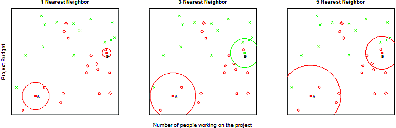
\includegraphics[width=0.7\linewidth]{ChapterML/figures/knn} 

}

\caption{Example of $k$-nearest neighbor with $k = 1, 3, 5$ neighbors. We want to predict the points A and B. The 1-nearest neighbor for both points is red ("Patent not granted"), the 3-nearest neighbor predicts point A (B) to be red (green) with probability 2/3, and the 5-nearest neighbor predicts again both points to be red with probabilities 4/5 and 3/5, respectively.}\label{fig:knn}
\end{figure}

Training for \(k\)-NN just means storing the data, making this method
useful in applications where data are coming in extremely quickly and a
model needs to be updated frequently. All the work, however, gets pushed
to scoring time, since all the distance calculations happen when a new
data point needs to be classified. There are several optimized methods
designed to make \(k\)-NN more efficient that are worth looking into if
that is a situation that is applicable to your problem.

In addition to selecting \(k\) and an appropriate distance metric, we
also have to be careful about the scaling of the features. When
distances between two data points are large for one feature and small
for a different feature, the method will rely almost exclusively on the
first feature to find the closest points. The smaller distances on the
second feature are nearly irrelevant to calculate the overall distance.
A similar problem occurs when continuous and categorical predictors are
used together. To resolve the scaling issues, various options for
rescaling exist. For example, a common approach is to center all
features at mean \(0\) and scale them to variance \(1\).

There are several variations of \(k\)-NN. One of these is weighted
nearest neighbors, where different features are weighted differently or
different examples are weighted based on the distance from the example
being classified. The method \(k\)-NN also has issues when the data are
sparse and has high dimensionality, which means that every point is far
away from virtually every other point, and hence pairwise distances tend
to be uninformative. This can also happen when a lot of features are
irrelevant and drown out the relevant features' signal in the distance
calculations.

Notice that the nearest-neighbor method can easily be applied to
regression problems with a real-valued target variable. In fact, the
method is completely oblivious to the type of target variable and can
potentially be used to predict text documents, images, and videos, based
on the aggregation function after the nearest neighbors are found.

\textbf{Support vector machines}

Support vector machines are one of the most popular and best-performing
classification methods in machine learning today. The mathematics behind
SVMs has a lot of prerequisites that are beyond the scope of this book,
but we will give you an intuition of how SVMs work, what they are good
for, and how to use them.

We are all familiar with linear models (e.g., logistic regression) that
separate two classes by fitting a line in two dimensions (or a
hyperplane in higher dimensions) in the middle (see Figure
\ref{fig:svm}). An important decision that linear models have to make is
which linear separator we should prefer when there are several we can
build.

\begin{figure}

{\centering 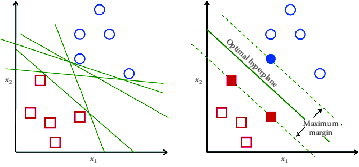
\includegraphics[width=1\linewidth]{ChapterML/figures/svm} 

}

\caption{Support vector machines}\label{fig:svm}
\end{figure}

You can see in Figure \ref{fig:svm} that multiple lines offer a solution
to the problem. Is any of them better than the others? We can
intuitively define a criterion to estimate the worth of the lines: A
line is bad if it passes too close to the points because it will be
noise sensitive and it will not generalize correctly. Therefore, our
goal should be to find the line passing as far as possible from all
points.

The SVM algorithm is based on finding the hyperplane that maximizes the
\emph{margin} of the training data. The training examples that are
closest to the hyperplane are called \emph{support vectors} since they
are \emph{supporting} the margin (as the margin is only a function of
the support vectors).

An important concept to learn when working with SVMs is \emph{kernels}.
SVMs are a specific instance of a class of methods called \emph{kernel
methods}. So far, we have only talked about SVMs as linear models.
Linear works well in high-dimensional data but sometimes you need
nonlinear models, often in cases of low-dimensional data or in image or
video data. Unfortunately, traditional ways of generating nonlinear
models get computationally expensive since you have to explicitly
generate all the features such as squares, cubes, and all the
interactions. Kernels are a way to keep the efficiency of the linear
machinery but still build models that can capture nonlinearity in the
data without creating all the nonlinear features.

You can essentially think of kernels as similarity functions and use
them to create a linear separation of the data by (implicitly) mapping
the data to a higher-dimensional space. Essentially, we take an
\(n\)-dimensional input vector \(X\), map it into a high-dimensional
(infinite-dimensional) feature space, and construct an optimal
separating hyperplane in this space. We refer you to relevant papers for
more detail on SVMs and nonlinear kernels (Shawe-Taylor and Cristianini
\protect\hyperlink{ref-ShaweTaylor2004}{2004}; Scholkopf and Smola
\protect\hyperlink{ref-Scholkopf2001}{2001}). SVMs are also related to
logistic regression, but use a different loss/penalty function (Hastie,
Tibshirani, and Friedman
\protect\hyperlink{ref-HastieTibshirani}{2001}).

When using SVMs, there are several parameters you have to optimize,
ranging from the \emph{regularization} parameter \(C\), which determines
the tradeoff between minimizing the training error and minimizing model
complexity, to more kernel-specific parameters. It is often a good idea
to do a grid search to find the optimal parameters. Another tip when
using SVMs is to normalize the features; one common approach to doing
that is to normalize each data point to be a vector of unit length.

Linear SVMs are effective in high-dimensional spaces, especially when
the space is sparse such as text classification where the number of data
points (perhaps tens of thousands) is often much less than the number of
features (a hundred thousand to a million or more). SVMs are also fairly
robust when the number of irrelevant features is large (unlike the
\(k\)-NN approaches that we mentioned earlier) as well as when the class
distribution is skewed, that is, when the class of interest is
significantly less than 50\% of the data.

One disadvantage of SVMs is that they do not directly provide
probability estimates. They assign a score based on the distance from
the margin. The farther a point is from the margin, the higher the
magnitude of the score. This score is good for ranking examples, but
getting accurate probability estimates takes more work and requires more
labeled data to be used to perform probability calibrations.

In addition to classification, there are also variations of SVMs that
can be used for regression (Smola and Schölkopf
\protect\hyperlink{ref-SmolaRegression04}{2004}) and ranking (Chapelle
and Keerthi \protect\hyperlink{ref-Chapelle2010}{2010}).

\textbf{Decision trees}

Decision trees are yet another set of methods that are helpful for
prediction. Typical decision trees learn a set of rules from training
data represented as a tree. An exemplary decision tree is shown in
Figure \ref{fig:tree}. Each level of a tree \emph{splits} the tree to
create a branch using a feature and a value (or range of values). In the
example tree, the first split is made on the feature \emph{number of
visits in the past year} and the value \(4\). The second level of the
tree now has two splits: one using \emph{average length of visit} with
value \(2\) days and the other using the value \(10\) days.

\begin{center}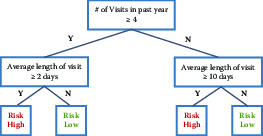
\includegraphics[width=0.7\linewidth]{ChapterML/figures/tree} \end{center}

\begin{figure}

{\centering 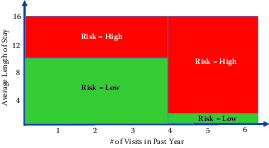
\includegraphics[width=0.7\linewidth]{ChapterML/figures/tree-rectangle} 

}

\caption{An exemplary decision tree. The top figure is the standard representation for trees. The bottom figure offers an alternative view of the same tree. The feature space is partitioned into numerous rectangles, which is another way to view a tree, representing its nonlinear character more explicitly}\label{fig:tree}
\end{figure}

Various algorithms exist to build decision trees. C4.5, CHAID, and CART
(Classification and Regression Trees) are the most popular. Each needs
to determine the next best feature to split on. The goal is to find
feature splits that can best reduce class impurity in the data, that is,
a split that will ideally put all (or as many as possible) positive
class examples on one side and all (or as many as possible) negative
examples on the other side. One common measure of impurity that comes
from information theory is \emph{entropy}, and it is calculated as
\[H(X) = -\sum_x p(x) \log p(x).\]

Entropy is maximum (1) when both classes have equal numbers of examples
in a node. It is minimum (0) when all examples are from the same class.
At each node in the tree, we can evaluate all the possible features and
select the one that most reduces the entropy given the tree so far. This
expected change in entropy is known as \emph{information gain} and is
one of the most common criteria used to create decision trees. Other
measures that are used instead of information gain are Gini and
chi-squared.

If we keep constructing the tree in this manner, selecting the next best
feature to split on, the tree ends up fairly deep and tends to overfit
the data. To prevent overfitting, we can either have a stopping
criterion or \emph{prune} the tree after it is fully grown. Common
stopping criteria include minimum number of data points to have before
doing another feature split, maximum depth, and maximum purity. Typical
pruning approaches use holdout data (or cross-validation, which will be
discussed later in this chapter) to cut off parts of the tree.

Once the tree is built, a new data point is classified by running it
through the tree and, once it reaches a terminal node, using some
aggregation function to give a prediction (classification or
regression). Typical approaches include performing maximum likelihood
(if the leaf node contains 10 examples, 8 positive and 2 negative, any
data point that gets into that node will get an 80\% probability of
being positive). Trees used for regression often build the tree as
described above but then fit a linear regression model at each leaf
node.

Decision trees have several advantages. The interpretation of a tree is
straightforward as long as the tree is not too large. Trees can be
turned into a set of rules that experts in a particular domain can
possibly dig deeper into, validate, and modify. Trees also do not
require too much feature engineering. There is no need to create
interaction terms since trees can implicitly do that by splitting on two
features, one after another.

Unfortunately, along with these benefits come a set of disadvantages.
Decision trees, in general, do not perform well, compared to SVMs,
random forests, or logistic regression. They are also unstable: small
changes in data can result in very different trees. The lack of
stability comes from the fact that small changes in the training data
may lead to different splitting points. As a consequence, the whole tree
may take a different structure. The suboptimal predictive performance
can be seen from the fact that trees partition the predictor space into
a few rectangular regions, each one predicting only a single value (see
the bottom part of Figure \ref{fig:tree}.

\textbf{Ensemble methods}

Combinations of models are generally known as model ensembles. They are
among the most powerful techniques in machine learning, often
outperforming other methods, although at the cost of increased
algorithmic and model complexity.

The intuition behind building ensembles of models is to build several
models, each somewhat different. This diversity can come from various
sources such as: training models on subsets of the data; training models
on subsets of the features; or a combination of these two.

Ensemble methods in machine learning have two things in common. First,
they construct multiple, diverse predictive models from adapted versions
of the training data (most often reweighted or resampled). Second, they
combine the predictions of these models in some way, often by simple
averaging or voting (possibly weighted).

\textbf{Bagging}

Bagging stands for ``bootstrap aggregation''\footnote{Bootstrap is a
  general statistical procedure that draws random samples of the
  original data with replacement.}: we first create bootstrap samples
from the original data and then aggregate the predictions using models
trained on each bootstrap sample. Given a data set of size \(N\), the
method works as follows:

\begin{enumerate}
\def\labelenumi{\arabic{enumi}.}
\item
  Create \(k\) bootstrap samples (with replacement), each of size \(N\),
  resulting in \(k\) data sets. Only about 63\% of the original training
  examples will be represented in any given bootstrapped set.
\item
  Train a model on each of the \(k\) data sets, resulting in \(k\)
  models.
\item
  For a new data point \(X\), predict the output using each of the \(k\)
  models.
\item
  Aggregate the \(k\) predictions (typically using average or voting) to
  get the prediction for \(X\).
\end{enumerate}

A nice feature of this method is that any underlying model can be used,
but decision trees are often the most commonly used base model. One
reason for this is that decision trees are typically high variance and
unstable, that is, they can change drastically given small changes in
data, and bagging is effective at reducing the variance of the overall
model. Another advantage of bagging is that each model can be trained in
parallel, making it efficient to scale to large data sets.

\textbf{Boosting}

Boosting is another popular ensemble technique, and it often results in
improving the base classifier being used. In fact, if your only goal is
improving accuracy, you will most likely find that boosting will achieve
that. The basic idea is to keep training classifiers iteratively, each
iteration focusing on examples that the previous one got wrong. At the
end, you have a set of classifiers, each trained on smaller and smaller
subsets of the training data. Given a new data point, all the
classifiers predict the target, and a weighted average of those
predictions is used to get the final prediction, where the weight is
proportional to the accuracy of each classifier. The algorithm works as
follows:

\begin{enumerate}
\def\labelenumi{\arabic{enumi}.}
\item
  Assign equal weights to every example.
\item
  For each iteration:

  \begin{enumerate}
  \def\labelenumii{\arabic{enumii}.}
  \item
    Train classifier on the weighted examples.
  \item
    Predict on the training data.
  \item
    Calculate error of the classifier on the training data.
  \item
    Calculate the new weighting on the examples based on the errors of
    the classifier.
  \item
    Reweight examples.
  \end{enumerate}
\item
  Generate a weighted classifier based on the accuracy of each
  classifier.
\end{enumerate}

One constraint on the classifier used within boosting is that it should
be able to handle weighted examples (either directly or by replicating
the examples that need to be overweighted). The most common classifiers
used in boosting are decision stumps (single-level decision trees), but
deeper trees can also work well.

Boosting is a common way to \emph{boost} the performance of a
classification method but comes with additional complexity, both in the
training time and in interpreting the predictions. A disadvantage of
boosting is that it is difficult to parallelize since the next iteration
of boosting relies on the results of the previous iteration.

A nice property of boosting is its ability to identify outliers:
examples that are either mislabeled in the training data, or are
inherently ambiguous and hard to categorize. Because boosting focuses
its weight on the examples that are more difficult to classify, the
examples with the highest weight often turn out to be outliers. On the
other hand, if the number of outliers is large (lots of noise in the
data), these examples can hurt the performance of boosting by focusing
too much on them.

\textbf{Random forests}

Given a data set of size \(N\) and containing \(M\) features, the random
forest training algorithm works as follows:

\begin{enumerate}
\def\labelenumi{\arabic{enumi}.}
\item
  Create \(n\) bootstrap samples from the original data of size \(N\).
  Remember, this is similar to the first step in bagging. Increasing
  \(n\) will lead to similar or better results, but also requires more
  computational resources. Typically \(n\) ranges from 100 to a few
  thousand but is best determined empirically.
\item
  For each bootstrap sample, train a decision tree using \(m\) features
  (where \(m\) is typically much smaller than \(M\)) at each node of the
  tree. The \(m\) features are selected uniformly at random from the
  \(M\) features in the data set, and the decision tree will select the
  best split among the \(m\) features. The value of \(m\) is held
  constant during the forest growing.
\item
  A new test example/data point is classified by all the trees, and the
  final classification is done by majority vote (or another appropriate
  aggregation method).
\end{enumerate}

Random forests often achieve remarkable results while being simple to
use. They can be easily parallelized, making them efficient to run on
large data sets, and can handle a large number of features, even with a
lot of missing values. Random forests can get complex, with hundreds or
thousands of trees that are fairly deep, so it is difficult to interpret
the learned model. At the same time, they provide a nice way to estimate
feature importance, giving a sense of what features were important in
building the classifier.

Another nice aspect of random forests is the ability to compute a
proximity matrix that gives the similarity between every pair of data
points. This is calculated by computing the number of times two examples
land in the same terminal node. The more that happens, the closer the
two examples are. We can use this proximity matrix for clustering,
locating outliers, or explaining the predictions for a specific example.

\textbf{Stacking}

Stacking is a technique that deals with the task of learning a
meta-level classifier to combine the predictions of multiple base-level
classifiers. This meta-algorithm is trained to combine the model
predictions to form a final set of predictions. This can be used for
both regression and classification. The algorithm works as follows:

\begin{enumerate}
\def\labelenumi{\arabic{enumi}.}
\item
  Split the data set into \(n\) equal-sized sets:
  \(set_1, set_2,\ldots,set_n\).
\item
  Train base models on all possible combinations of \(n-1\) sets and,
  for each model, use it to predict on \(set_i\) what was left out of
  the training set. This would give us a set of predictions on every
  data point in the original data set.
\item
  Now train a second-stage stacker model on the predicted classes or the
  predicted probability distribution over the classes from the
  first-stage (base) model(s).
\end{enumerate}

By using the first-stage predictions as features, a stacker model gets
more information on the problem space than if it were trained in
isolation. The technique is similar to cross-validation, an evaluation
methodology that we will cover later in this chapter.

\textbf{Neural networks and deep learning}

Neural networks are a set of multi-layer classifiers where the outputs
of one layer feed into the inputs of the next layer. The layers between
the input and output layers are called \emph{hidden layers}, and the
more hidden layers a neural network has, the more complex functions it
can learn. Neural networks were popular in the 1980s and early 1990s,
but then fell out of fashion because they were slow and expensive to
train, even with only one or two hidden layers. Since 2006, a set of
techniques has been developed that enable learning in deeper neural
networks. These techniques, with access to massive computational
resources and large amounts of data, have enabled much deeper (and
larger) networks to be Trained and it turns out that these perform far
better on many problems than shallow neural networks (with just a single
hidden layer). The reason for the better performance is the ability of
deep nets to build up a complex hierarchy of concepts, learning multiple
levels of representation and abstraction that help to make sense of data
such as images, sound, and text.

There are a few different types of neural networks that are popular
today:

\begin{itemize}
\item
  Convolutional Neural Networks (\textbf{CNN}s): These are often used in
  detecting objects in images and in doing image search, but their
  applicability goes beyond just image analysis and they can be used to
  find patterns in other types of data as well. CNNs treat input data
  (such as images) in a spatial manner (in two or three dimensions for
  example), and are able to capture spatial dependencies in the data.
\item
  Recurrent Neural Networks (\textbf{RNN}s): are suitable for modeling
  sequential data that has temporal dependencies. They are trained to
  generate the next steps in a sequence, such as the next letters in a
  word, or the next words in a sentence, voice recording, or video. They
  are typically used in translation, speech generation, and time series
  prediction tasks. A popular variation of RNNs is LSTM (Long Short Term
  Memory) that are used because of their ability and effectiveness in
  modeling long-range dependencies.
\item
  Generative Adversarial Network (\textbf{GAN}s): have been shown to be
  quite adept at generating new, realistic images based on other
  training images. GANs train two models in parallel. One network
  (called generator) is trained to generate data (based on historical
  examples of previously occurring data such as images or text or
  video). The other network (discriminator) tries to classify these
  generated images as real or synthetic. During training a GAN, the goal
  is to generate data that is realistic enough that the discriminator
  network is fooled to the point that it cannot distinguish the
  difference between the real and the synthetic input data.
\end{itemize}

Goodfellow et al. (\protect\hyperlink{ref-Goodfellow2016}{2016}) provide
a (mathematical) introduction to deep learning.

Currently, deep neural networks are popular for a certain class of
problems and a lot of research is being done on them. It is, however,
important to keep in mind that they may often require a lot more data
than are available in many problems. In many problems, such as natural
language processing, image, and video analysis, there are techniques to
start from a pre-trained neural network model, that reduces the need for
additional training data. Training deep neural networks also requires a
lot of computational power, but that is less likely to be an issue for
most people today with increased access to computing resources. Typical
cases where deep learning has been shown to be effective involve lots of
images, video, and text data. We are in the early stages of development
of this class of methods, and although there seems to be a lot of
potential, we need a much better understanding of why they are effective
and the problems for which they are well suited.

\subsection{Binary vs Multiclass classification
problems}\label{binary-vs-multiclass-classification-problems}

In the discussion above, we framed classification problems as binary
classification problems with a 0 or 1 output. There are many problems
where we have multiple classes, such as classifying companies into their
industry codes or predicting whether a student will drop out, transfer,
or graduate. Several solutions have been designed to deal with the
multiclass classification problem:

\begin{itemize}
\item
  \textbf{Direct multiclass}: Use methods that can directly perform
  multiclass classification. Examples of such methods are \(K\)-nearest
  neighbor, decision trees, and random forests. There are extensions of
  support vector machines that exist for multiclass classification as
  well (Crammer and Singer \protect\hyperlink{ref-crammer2002}{2002}),
  but they can often be slow to train.
\item
  \textbf{Convert to one versus all (OVA)}: This is a common approach to
  solve multiclass classification problems using binary classifiers. Any
  problem with \(n\) classes can be turned into \(n\) binary
  classification problems, where each classifier is trained to
  distinguish between one versus all the other classes. A new example
  can be classified by combining the predictions from all the \(n\)
  classifiers and selecting the class with the highest score. This is a
  simple and efficient approach, and one that is commonly used, but it
  suffers from each classification problem possibly having an imbalanced
  class distribution (due to the negative class being a collection of
  multiple classes). Another limitation of this approach is that it
  requires the scores of each classifier to be calibrated so that they
  are comparable across all of them.
\item
  \textbf{Convert to pairwise}: In this approach, we can create binary
  classifiers to distinguish between each pair of classes, resulting in
  \(\binom{n}{2}\) binary classifiers. This results in a large number of
  classifiers, but each classifier usually has a balanced classification
  problem. A new example is classified by taking the predictions of all
  the binary classifiers and using majority voting.
\end{itemize}

\subsection{Skewed or imbalanced classification
problems}\label{skewed-or-imbalanced-classification-problems}

A lot of problems you will deal with will not have uniform (balanced)
distributions for both classes. This is often the case with problems in
fraud detection, network security, and medical diagnosis where the class
of interest is not very common. The same is true in many social science
and public policy problems around behavior prediction, such as
predicting which students will not graduate on time, which children may
be at risk of getting lead poisoning, or which homes are likely to be
abandoned in a given city. You will notice that applying standard
machine learning methods may result in all the predictions being for the
most frequent category in such situations, making it problematic to
detect the infrequent classes. There has been a lot of work in machine
learning research on dealing with such problems (Chawla
\protect\hyperlink{ref-Chawla05}{2005}; Kuhn and Johnson
\protect\hyperlink{ref-KuhnJohnson2013}{2013}) that we will not cover in
detail here. Common approaches to deal with class imbalance include
oversampling from the minority class and undersampling from the majority
class. It is important to keep in mind that the sampling approaches do
not need to result in a \(1:1\) ratio. Many supervised learning methods
described in this chapter (such as Random Forests and SVMs) can work
well even with a \(10:1\) imbalance. Also, it is critical to make sure
that you only resample the training set; keep the distribution of the
test set the same as that of the original data since you will not know
the class labels of new data in practice and will not be able to
resample.

\subsection{Model interpretability}\label{model-interpretability}

As social scientists (or good machine learning practitioners), we do not
only care about building machine learning models but also want to
understand what the models ``learned'', and how to use them to make
inferences and decisions. Understanding, or interpreting machine
learning models is a key requirement for most social science and policy
problems. There are various reasons for this including:

\begin{itemize}
\tightlist
\item
  Providing information that can help in debugging and improving models
\item
  Increasing trust in the models and hence increasing their adoption by
  decisionmakers
\item
  Improving the decisions being made using the models by reinforcing the
  correct predictions and helping the decision-maker override the wrong
  predictions.
\item
  Helping select appropriate interventions based on the explanations
\item
  Providing legal recourse to people being affected by the decisions
  made using the models
\end{itemize}

\textbf{Global versus Individual-Level Explanations}

When thinking about model interpretability, there are two types of
interpretability:

\begin{itemize}
\tightlist
\item
  Global: At the overall model level
\item
  Individual: Explaining an individual classification/prediction that is
  made by a model.
\end{itemize}

Both of these are important for different reasons. We need global
interpretability to help understand the overall model but we also need
explanations for individual classifications when these models are
helping a person make decisions about individual cases. A social worker
identifying the risk of a client going back to the homeless shelter and
determining appropriate interventions to reduce that risk, or a
counselor in an employment agency determining how likely an individual
is to be long-term unemployed and connecting them with appropriate
training programs or job opportunities need individual-level
explanations of predictions/recommendations that the machine learning
model is generating.

\emph{Global Interpretability}

Each method results in a model that needs to be interpreted in a way
that is appropriate for that method. For example, for a decision tree,
we may want to view the tree to understand what types of classifications
are being made. This can of course get cumbersome and difficult if the
tree is extremely large. For logistic regression models, we can look at
the coefficients and odds-ratios, but it is often difficult to mentally
account for different variables controlling for each other. In general,
the models discussed above have different ways of exposing their
``feature importances''\^{}{[}Some measure of how useful that feature
was for the given model.{]} and we often use that as a proxy for global
model interpretability.

Another way of interpreting a model is to understand how the model
scores individual data points. We can take the set of entities that are
scored by the model, and generate cross-tabs that highlight how the top
x\% of the scored/predicted entities are different from the rest of the
entities. This approach allows us to get an idea of what the model is
doing, not in general, but on the entities of interest to us and makes
interpretability a little more intuitive and generalizable across
different model types.

A different approach that some have taken in this area has been to
sparse\^{}{[}Using a small number of features/predictors.{]} models,
making them easier to interpret. The motivation behind these simple,
sparse models is that they are inherently interpretble and do not
require the use of additional analysis for humans to understand them.
Examples of such work include Ustun and Rudin
(\protect\hyperlink{ref-Ustun2019}{2019}), Ustun and Rudin
(\protect\hyperlink{ref-Ustun2016}{2016}), and Caruana et al.
(\protect\hyperlink{ref-Caruana2015}{2015}). These models may not
perform well in every task so it's important for us to explore the range
of models in terms of performance and complexity, and decide what level
and type of interpretability we need and how to balance that with the
accuracy\footnote{We are using accuracy as a proxy for different
  confusion-matrix based performance metrics such as precision, recall,
  etc.} of those models.

\emph{Individual-Level Explanations}

While it's important to understand the models we are building at a
global level, in many social science applications, we want to get an
explanation for why a data point was classified/predicteda certain way
by the model. There has been a lot of recent work on methods for
generating individual-level explanations for predictions made by machine
learning models. These fall into two areas: 1. Model specific methods:
These are used to generate explanations for predictions made by a
specific class of methods, such as neural networks or random forests. 2.
Model agnostic methods: These can be used to generate explanations for
individual predictions made by any type of model. Examples of this
include LIME (Ribeiro, Singh, and Guestrin
\protect\hyperlink{ref-ribeiro-16}{2016}), MAPLE (Plumb, Molitor, and
Talwalkar \protect\hyperlink{ref-Plumb2018}{2018}), and SHAP values
(Lundberg and Lee \protect\hyperlink{ref-Lundberg2017}{2017}).

It's important to keep in mind though that these ``explanations'' are
typically not causal, and are often restricted to be a ranked list of
``features''. One way to think about them is that these features were
most important in assigning this data point the score it was given by a
particular model. This is currently an active area of machine learning
research and will hopefully mature into a set of methods and tools
useful for social scientists using machine learning to solve problems
that require a better and deeper understanding of their predictions.

\section{Evaluation}\label{sec:7-7}

The previous section introduced us to a variety of methods, all with
certain pros and cons, and no single method guaranteed to outperform
others for a given problem. This section focuses on evaluation methods,
with three primary goals:

\begin{enumerate}
\def\labelenumi{\arabic{enumi}.}
\item
  Model selection: How do we select a method to use in the future? What
  parameters should we select for that method?
\item
  Performance estimation: How do we estimate how well our model will
  perform once it is deployed and applied to new data?
\item
  A deeper understanding of the types of models that work well and those
  that don't can point to the effectiveness and applicability of
  existing methods and provide a better understanding of the structure
  of the data and the problem we are tackling.
\end{enumerate}

This section will cover evaluation methodologies as well as metrics that
are commonly used.

\subsection{Methodology}\label{sec:7-7.1}

\textbf{In-sample evaluation}

As social scientists, you already evaluate methods on how well they
perform in-sample (on the set that the model was trained on). As we
mentioned earlier in the chapter, the goal of machine learning methods
is to generalize to new data, and validating models in-sample does not
allow us to do that. We focus here on evaluation methodologies that
allow us to optimize (as best as we can) for generalization performance.
The methods are illustrated in Figure \ref{fig:holdout}.

\textbf{Out-of-sample and holdout set}

The simplest way to focus on generalization is to \emph{pretend} to
generalize to new (unseen) data. One way to do that is to take the
original data and randomly split them into two sets: a \emph{training
set} and a \emph{test set} (sometimes also called the \emph{holdout} or
\emph{validation set}). We can decide how much to keep in each set
(typically the splits range from 50--50 to 80--20, depending on the size
of the data set). We then train our models on the training set and
classify the data in the test set, allowing us to get an estimate of the
relative performance of the methods.

One drawback of this approach is that we may be extremely lucky or
unlucky with our random split. One way to get around the problem that is
to repeatedly create multiple training and test sets. We can then train
on \(TR_1\) and test on \(TE_1\), train on \(TR_2\) and test on
\(TE_2\), and so on. The performance measures on each test set can then
give us an estimate of the performance of different methods and how much
they vary across different random sets.

\begin{figure}

{\centering 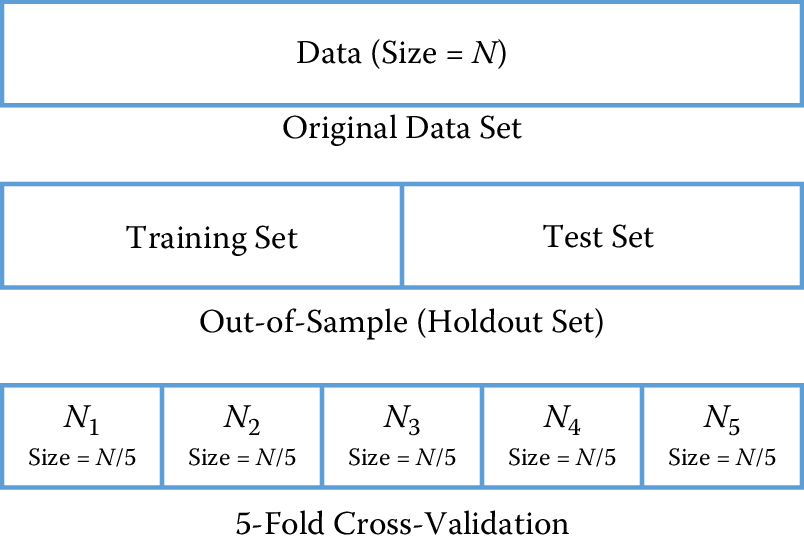
\includegraphics[width=0.7\linewidth]{ChapterML/figures/holdout} 

}

\caption{Validation methodologies: holdout set and cross-validation}\label{fig:holdout}
\end{figure}

\textbf{Cross-validation}

Cross-validation is a more sophisticated holdout training and testing
procedure that takes away some of the shortcomings of the holdout set
approach. Cross-validation begins by splitting a labeled data set into
\(k\) partitions (called folds). Typically, \(k\) is set to \(5\) or
\(10\). Cross-validation then proceeds by iterating \(k\) times. In each
iteration, one of the \(k\) folds is held out as the test set, while the
other \(k-1\) folds are combined and used to train the model. A nice
property of cross-validation is that every example is used in one test
set for testing the model. Each iteration of cross-validation gives us a
performance estimate that can then be aggregated (typically averaged) to
generate the overall estimate.

An extreme case of cross-validation is called leave-one-out
cross-validation, where given a data set of size \(N\), we create \(N\)
folds. That means iterating over each data point, holding it out as the
test set, and training on the rest of the \(N-1\) examples. This
illustrates the benefit of cross-validation by giving us good
generalization estimates (by training on as much of the data set as
possible) and making sure the model is tested on each data point.

\textbf{Temporal validation}

The cross-validation and holdout set approaches described above assume
that the data have no time dependencies and that the distribution is
stationary over time. This assumption is almost always violated in
practice and affects performance estimates for a model.

\begin{figure}

{\centering 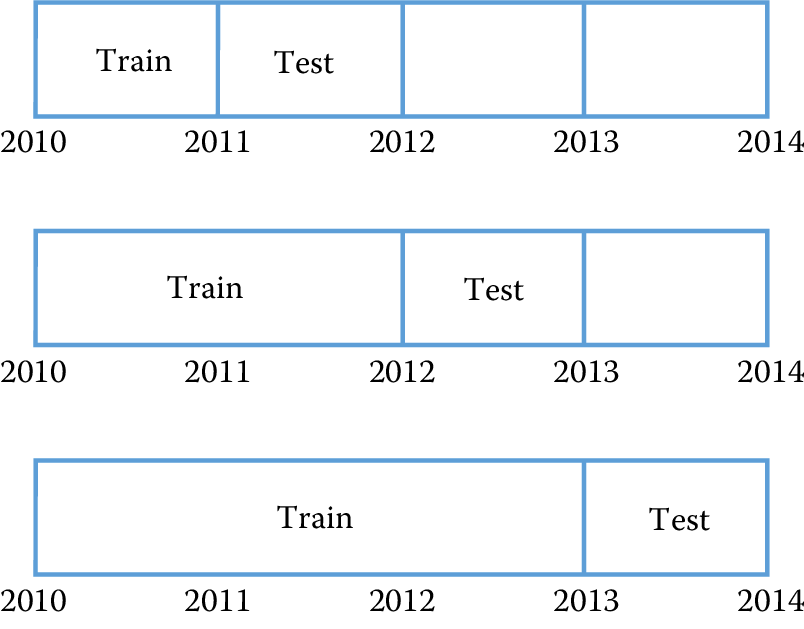
\includegraphics[width=0.7\linewidth]{ChapterML/figures/temporal} 

}

\caption{Temporal validation}\label{fig:temporal}
\end{figure}

In most practical problems, we want to use a validation strategy that
emulates the way in which our models will be used and provides an
accurate performance estimate. We will call this \emph{temporal
validation}. For a given point in time \(t_i\), we train our models only
on information available to us before \(t_i\) to avoid training on data
from the ``future.'' We then predict and evaluate on data from \(t_i\)
to \(t_i\) + \(d\) and iterate, expanding the training window while
keeping the test window size constant at \(d\). Figure
\ref{fig:temporal} shows this validation process with \(t_i=2010\) and
\(d=1\) year. The test set window \(d\) depends on a few factors related
to how the model will be deployed to best emulate reality:

\begin{enumerate}
\def\labelenumi{\arabic{enumi}.}
\item
  How far out in the future do predictions need to be made? For example,
  if the set of students who need to be targeted for interventions has
  to be finalized at the beginning of the school year for the entire
  year, then \(d = 1\) year.
\item
  How often will the model be updated? If the model is being updated
  daily, then we can move the window by a day at a time to reflect the
  deployment scenario.
\item
  How often will the system get new data? If we are getting new data
  frequently, we can make predictions more frequently.
\end{enumerate}

Temporal validation is similar to how time series models are evaluated
(also known as backtesting) and should be the validation approach used
for most practical problems.

\subsection{Metrics}\label{sec:7-7.2}

The previous subsection focused on validation methodologies assuming we
have an evaluation metric in mind. This section will go over commonly
used evaluation metrics. You are probably familiar with using \(R^2\),
analysis of the residuals, and mean squared error (MSE) to evaluate the
quality of regression models. For regression problems, the MSE
calculates the average squared differences between predictions
\(\hat{y}_i\) and true values \(y_i\). When prediction models have
smaller MSE, they are better. However, the MSE itself is hard to
interpret because it measures quadratic differences. Instead, the root
mean squared error (RMSE) is more intuitive as it as measure of mean
differences on the original scale of the response variable. Yet another
alternative is the mean absolute error (MAE), which measures average
absolute distances between predictions and true values.

We will now describe some additional evaluation metrics commonly used in
machine learning for classification. Before we dive into metrics, it is
important to highlight that machine learning models for classification
typically do not predict 0/1 values directly. SVMs, random forests, and
logistic regression all produce a score (which is sometimes a
probability) that is then turned into 0 or 1 based on a user-specific
threshold. You might find that certain tools (such as
scikitlearn\footnote{You should never use the predict function in
  sci-kit-learn since it assumes a 0.5 threshold.}) use a default value
for that threshold (often 0.5), but it is important to know that it is
an arbitrary threshold and you should select the threshold based on the
data, the model, and the problem you are solving. We will cover that a
little later in this section.

Once we have turned the real-valued predictions into 0/1 classification,
we can now create a \emph{confusion matrix} from these predictions,
shown in Figure \ref{fig:cm}. Each data point belongs to either the
positive class or the negative class, and for each data point the
prediction of the classifier is either correct or incorrect. This is
what the four cells of the confusion matrix represent. We can use the
confusion matrix to describe several commonly used evaluation metrics.

\begin{figure}

{\centering 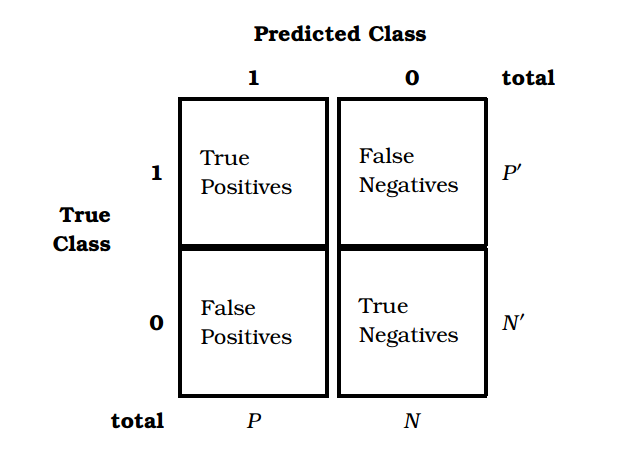
\includegraphics[width=0.7\linewidth]{ChapterML/figures/cm} 

}

\caption{A *confusion matrix* created from real-valued predictions}\label{fig:cm}
\end{figure}

Accuracy is the ratio of correct predictions (both positive and
negative) to all predictions:
\[\textrm{Accuracy}=\frac{TP + TN}{TP + TN + FP + FN}=\frac{TP + TN}{P+N}=\frac{TP + TN}{P'+N'},\]
where \(TP\) denotes true positives, \(TN\) true negatives, \(FP\) false
positives, \(FN\) false negatives, and other symbols denote row or
column totals. Accuracy is the most commonly described evaluation metric
for classification but is surprisingly the least useful in practical
situations (at least by itself). One problem with accuracy is that it
does not give us an idea of \emph{lift} compared to baseline. For
example, if we have a classification problem with 95\% of the data as
positive and 5\% as negative, a classifier with 85\% is performing worse
than a dumb classifier that predicts positive all the time (and will
have 95\% accuracy).

Two additional metrics that are often used are precision and recall,
which are defined as follows: \[\begin{aligned}
{\rm Precision} &= \frac{TP}{TP + FP}=\frac{TP}{P},
\\
{\rm Recall} &= \frac{TP}{TP + FN}=\frac{TP}{P'}
\end{aligned}\] (see also Box \protect\hyperlink{box:ml3}{Vocabulary}).
Precision measures the accuracy of the classifier when it predicts an
example to be positive. It is the ratio of correctly predicted positive
examples (\(TP\)) to all examples predicted as positive (\(TP + FP\)).
This measure is also called \emph{positive predictive value} in other
fields. Recall measures the ability of the classifier to find positive
examples. It is the ratio of all the correctly predicted positive
examples (\(TP\)) to all the positive examples in the data
(\(TP + FN\)). This is also called \emph{sensitivity} in other fields.

You might have encountered another metric called \emph{specificity} in
other fields. This measure is the true negative rate: the proportion of
negatives that are correctly identified.

Another metric that is used is the \(F_1\) score, which is the harmonic
mean of precision and recall:
\[F_1 =  \frac{2* {\rm Precision} * {\rm Recall}}{{\rm Precision} + {\rm Recall}}\]

This is often used when you want to balance both precision and recall.

There is often a tradeoff between precision and recall. By selecting
different classification thresholds, we can vary and tune the precision
and recall of a given classifier. A highly conservative classifier that
only predicts a 1 when it is absolutely sure (say, a threshold of
0.9999) will most often be correct when it predicts a 1 (high precision)
but will miss most 1s (low recall). At the other extreme, a classifier
that says 1 to every data point (a threshold of 0.0001) will have
perfect recall but low precision. Figure \ref{fig:pr} show a
precision--recall curve that is often used to represent the performance
of a given classifier.

\begin{figure}

{\centering 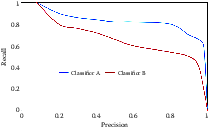
\includegraphics[width=0.7\linewidth]{ChapterML/figures/pr} 

}

\caption{Precision--recall curve}\label{fig:pr}
\end{figure}

\begin{figure}

{\centering 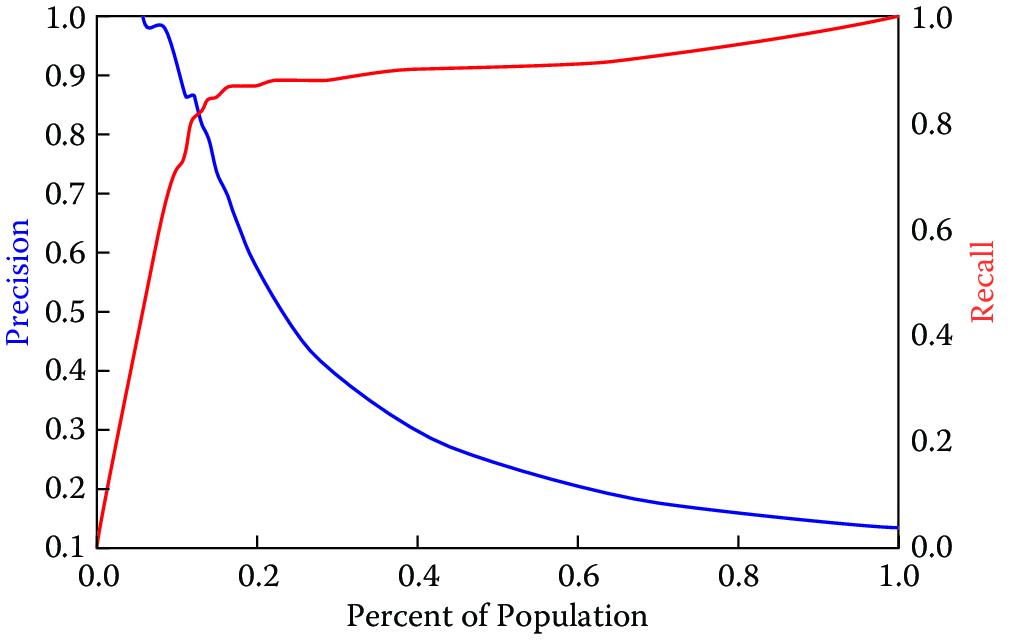
\includegraphics[width=0.7\linewidth]{ChapterML/figures/pr2} 

}

\caption{Precision or recall at different thresholds}\label{fig:pr2}
\end{figure}

If we care about optimizing for the entire precision recall space, a
useful metric is the \emph{area under the curve} (AUC-PR), which is the
area under the precision--recall curve. AUC-PR must not be confused with
AUC-ROC, which is the area under the related receiver operating
characteristic (ROC) curve. The ROC curve is created by plotting recall
versus (1 -- specificity). Both AUCs can be helpful metrics to compare
the performance of different methods and the maximum value the AUC can
take is 1. If, however, we care about a specific part on the
precision--recall curve, we have to look at finer-grained metrics.

Let us consider an example from public health. Most public health
agencies conduct inspections of various sorts to detect health hazard
violations (lead hazards, for example). The number of possible places
(homes or businesses) to inspect far exceeds the inspection resources
typically available. Let us assume further that they can only inspect
5\% of all possible places; they would clearly want to prioritize the
inspection of places that are most likely to contain the hazard. In this
case, the model will score and rank all the possible inspection places
in order of hazard risk. We would then want to know what percentage of
the top 5\% (the ones that will get inspected) are likely to be hazards,
which translates to the precision in the top 5\% of the most confidence
predictions---precision at 5\%, as it is commonly called (see Figure
\ref{fig:pr2}). \emph{Precision at top k percent} is a common class of
metrics widely used in information retrieval and search engine
literature, where you want to make sure that the results retrieved at
the top of the search results are accurate. More generally, this metric
is often used in problems in which the class distribution is skewed and
only a small percentage of the examples will be examined manually
(inspections, investigations for fraud, etc.). The literature provides
many case studies of such applications (Kumar, Ghani, and Mei
\protect\hyperlink{ref-Kumar2010}{2010}; Lakkaraju et al.
\protect\hyperlink{ref-Lakkaraju2015}{2015}; Potash et al.
\protect\hyperlink{ref-Potash2015}{2015}).

One last metric we want to mention is a class of cost-sensitive metrics
where different costs (or benefits) can be associated with the different
cells in the confusion matrix. So far, we have implicitly assumed that
every correct prediction and every error, whether for the positive class
or the negative class, has equal costs and benefits. In many practical
problems, that is not the case. For example, we may want to predict
whether a patient in a hospital emergency room is likely to go into
cardiac arrest in the next six hours. The cost of a false positive in
this case is the cost of the intervention (which may be a few extra
minutes of a physician's time) while the cost of a false negative could
be death. This type of analysis allows us to calculate the expected
value of the predictions of a classifier and select the model that
optimizes this cost-sensitive metric.

\section{Practical tips}\label{practical-tips}

Here we highlight some practical tips that will be helpful when using
machine learning.

\subsection{Avoiding Leakage}\label{avoiding-leakage}

Leakage is when your model has access to data at training/building time
that it wouldn't have at test/deployment/prediction time. The result is
an overoptimistic model that performs much worse when deployed.

The most common forms of leakage happen because of temporal issues --
including data from the future in your model because you have that when
you're doing model selection but there are many other ways leakage gets
introduced. Here are the most common ones

\textbf{The Big (and obvious) One}

\begin{enumerate}
\def\labelenumi{\arabic{enumi}.}
\tightlist
\item
  Using a proxy for the outcome variable (label) as a feature. This one
  is often easy to detect because you get perfect performance but is
  more nuanced when the proxy is some approximation of the label/outcome
  variable and the performance increase is more subtle to detect easily.
\end{enumerate}

\textbf{Doing any transformation or inference using the entire dataset}

\begin{enumerate}
\def\labelenumi{\arabic{enumi}.}
\setcounter{enumi}{1}
\item
  Using the entire data set for Imputations. Always do imputation based
  on your training set only, for each training set. Including the test
  set allows information to leak in to your models, especially in cases
  where the world changes in the future (when does it not?!)
\item
  Using the entire data set for discretizations or
  normalizations/scaling or many other data-based transformations. Same
  reason as \#2. The range of a variable (age for example) can change in
  the future and knowing that will make your models do/look better than
  they actually are.
\item
  Using the entire data set for Feature Selection. Same reasons as \#2
  and \#3. To play it safe, first split into train and test sets, and
  then do everything you need to do using that data.
\end{enumerate}

\textbf{Using information from the future (that will not available at
training or prediction time)}

\begin{enumerate}
\def\labelenumi{\arabic{enumi}.}
\setcounter{enumi}{4}
\item
  Using (proxies/transformation of) future outcomes as features: Similar
  to \#1
\item
  Doing standard k fold cross-validation when you have temporal data. If
  you have temporal data (that is non-stationary---again, when is it
  not!), k-fold cross validation will shuffle the data and a training
  set will (probably) contain data from the future and a test set will
  (probably) contain data from the past.
\item
  Using data (as features) that happened before model training time but
  is not available until later. This is fairly common in cases where
  there is lag/delay in data collection or access. An event may happen
  today but it doesn't appear in the database until a week, a month, or
  a year later and while it will be available in the data set you're
  using to build and select ML models, it will not be available at
  prediction time in deployment.
\item
  Using data (as rows) in the training set based on information from the
  future. Including rows that match certain criteria (in the future) in
  the training set, such as everyone who got a social service in the
  next 3 months) leaks information to your model via a biased training
  set.
\end{enumerate}

\textbf{Humans using knowledge from the future}

\begin{enumerate}
\def\labelenumi{\arabic{enumi}.}
\setcounter{enumi}{8}
\tightlist
\item
  Selecting certain models, features, and other design choices that are
  based on humans (ML developers, domain experts) knowing what happened
  in the future. This is a gray area -- we do want to use all of our
  domain knowledge to build more effective systems but sometimes that
  may not generalize into the future and result in
  overfitted/over-optimistic models at training time and disappointment
  once they're deployed.
\end{enumerate}

As a general rule, if you encounter a machine learning model that is
performing really well, it's probably because you've made an error that
is resulting in leakage. One way to dig deeper is to look at the feature
importances of your model to see if the most important feature(s) may be
the source of that leakage.

\subsection{Machine learning pipeline}\label{machine-learning-pipeline}

When working on machine learning projects, it is a good idea to
structure your code as a modular pipeline so you can easily try
different approaches and methods without major restructuring. The Python
workbooks supporting this book will give you an example of a machine
learning pipeline.\footnote{See
  \url{https://workbooks.coleridgeinitiative.org}.} A good pipeline will
contain modules for importing data, doing exploration, feature
generation, classification, and evaluation. You can then instantiate a
specific workflow by combining these modules.

An important component of the machine learning pipeline is comparing
different methods. With all the methods out there and all the
hyperparameters they come with, how do we know which model to use and
which hyperparameters to select? And what happens when we add new
features to the model or when the data have ``temporal drift'' and
change over time? One simple approach is to have a nested set of loops
that loop over all the methods you have access to, then enumerate all
the hyperparameters for that method, create a cross-product, and loop
over all of them, comparing them across different evaluation metrics and
selecting the best one to use going forward. You can even add different
feature subsets and time slices to this loop, as the example in the
supporting workbooks will show. Triage
(\url{http://github.com/dssg/triage}) is a good example of a machine
learning pipeline that is designed to solve many public policy problems.

\section{How can social scientists benefit from machine
learning?}\label{how-can-social-scientists-benefit-from-machine-learning}

In this chapter, we have introduced you to some new methods (both
unsupervised and supervised), validation methodologies, and evaluation
metrics. All of these can benefit social scientists as they tackle
problems in research and practice. In this section, we will give a few
concrete examples where what you have learned so far can be used to
improve some social science tasks:

\begin{itemize}
\item
  \textbf{Use of better prediction methods and methodology}: Traditional
  statistics and social sciences have not focused much on methods for
  prediction. Machine learning researchers have spent the past 30 years
  developing and adapting methods focusing on that task. We believe that
  there is a lot of value for social science researchers and
  practitioners in learning more about those methods, applying them, and
  even augmenting them (Kleinberg et al.
  \protect\hyperlink{ref-Kleinberg2015}{2015}). Two common tasks that
  can be improved using better prediction methods are generating
  counterfactuals (essentially a prediction problem) and matching. In
  addition, holdout sets and cross-validation can be used as a model
  selection methodology with any existing regression and classification
  methods, resulting in improved model selection and error estimates.
\item
  \textbf{Model misspecification}: Linear and logistic regressions are
  common techniques for data analysis in the social sciences. One
  fundamental assumption within both is that they are additive over
  parameters. Machine learning provides tools when this assumption is
  too limiting. Hainmueller and Hazlett
  (\protect\hyperlink{ref-hainmueller2014kernel}{2014}), for example,
  reanalyze data that were originally analyzed with logistic regression
  and come to substantially different conclusions. They argue that their
  analysis, which is more flexible and based on supervised learning
  methodology, provides three additional insights when compared to the
  original model. First, predictive performance is similar or better,
  although they do not need an extensive search to find the final model
  specification as it was done in the original analysis. Second, their
  model allows them to calculate average marginal effects that are
  mostly similar to the original analysis. However, for one covariate
  they find a substantially different result, which is due to model
  misspecification in the original model. Finally, the reanalysis also
  discovers interactions that were missed in the original publication.
\item
  \textbf{Better text analysis}: Text is everywhere, but unfortunately
  humans are slow and expensive in analyzing text data. Thus, computers
  are needed to analyze large collections of text. Machine learning
  methods can help make this process more efficient. Feldman and Sanger
  (\protect\hyperlink{ref-FeldmanSanger}{2006}) provide an overview of
  different automatic methods for text analysis. Grimmer and Stewart
  (\protect\hyperlink{ref-grimmer2013text}{2013}) give examples that are
  more specific for social scientists, and Chapter
  \protect\hyperlink{chap:text}{Text analysis} provides more details on
  this topic.
\item
  \textbf{Adaptive surveys}: Some survey questions have a large number
  of possible answer categories. For example, international job
  classifications describe more than 500 occupational categories, and it
  is prohibitive to ask all categories during the survey. Instead,
  respondents answer an open-ended question about their job and machine
  learning algorithms can use the verbatim answers to suggest small sets
  of plausible answer options. The respondents can then select which
  option is the best description for their occupation, thus saving the
  costs for coding after the interview (Schierholz et al.
  \protect\hyperlink{ref-Schierholz2018}{2018}).
\item
  \textbf{Estimating heterogeneous treatment effects}: A standard
  approach to causal inference is the assignment of different treatments
  (e.g., medicines) to the units of interest (e.g., patients).
  Researchers then usually calculate the average treatment effect---the
  average difference in outcomes for both groups. It is also of interest
  if treatment effects differ for various subgroups (e.g., is a medicine
  more effective for younger people?). Traditional subgroup analysis has
  been criticized and challenged by various machine learning techniques
  (Green and Kern \protect\hyperlink{ref-green2012modeling}{2012}; Imai,
  Ratkovic, and others
  \protect\hyperlink{ref-imai2013estimating}{2013}).
\item
  \textbf{Variable selection}: Although there are many methods for
  variable selection, regularized methods such as the lasso are highly
  effective and efficient when faced with large amounts of data. Varian
  (\protect\hyperlink{ref-Varian2014}{2014}) goes into more detail and
  gives other methods from machine learning that can be useful for
  variable selection. We can also find interactions between pairs of
  variables (to feed into other models) using random forests, by looking
  at variables that co-occur in the same tree, and by calculating the
  strength of the interaction as a function of how many trees they
  co-occur in, how high they occur in the trees, and how far apart they
  are in a given tree.
\end{itemize}

\section{Advanced topics}\label{advanced-topics}

This has been a short but intense introduction to machine learning, and
we have left out several important topics that are useful and
interesting for you to know about and that are being actively researched
in the machine learning community. We mention them here so you know what
they are, but will not describe them in detail. These include:

\begin{itemize}
\item
  Semi-supervised learning, where a combination of labeled and unlabeled
  data are used for training, given a set of assumptions. Such methods
  are useful when labeling data is costly and where unlabeled (not
  manually labeled/tagged data) can help improve the machine learning
  models. See the MIT Press edited volume (Chapelle, Schoelkopf, and
  Zien \protect\hyperlink{ref-Chapelle2006}{2006}) for explanations and
  examples.
\item
  Recommender systems: These are commonly used by audio and video
  services like YouTube to generate playlists or by online shops like
  Amazon to suggest additional products a custumer might wish to buy.
  More generally, recommender systems aim to predict the preferences a
  user might have. One strategy is to recommend products that have
  similar characteristcs to the ones already selected by the same user
  (independent of others). Another strategy recommends a product if
  other persons with a similar profile selected the same product in the
  past.
\item
  Active learning, a set of machine learning algorithms that query the
  user or some other information source to get labels for data points
  that are most beneficial for the machine learning models. This is in
  contrast to the standard machine learning process where we often
  select data points to label/tag randomly. Active Learning approaches
  to selecting data points to label have been shown to reduce the effort
  needed to train machine learning models.
\item
  Reinforcement learning: The ``supervised`` machine learning methods
  we've covered in this chapter are ``one-shot'' and take data points
  and labels as inputs. Reinforcement Learning is a different machine
  learning paradigm where the machine learning program takes a series of
  actions/decisions, and gets delayed feedback (reward or penalty) when
  performing a task. The goal of reinforcement learning is to determine
  the next best action to take in order to maximize long term
  performance. This has been applied to scenarios such as playing games
  (checkers, chess, backgammon, etc.) and in robotics (Sutton and Barto
  \protect\hyperlink{ref-Sutton2018}{2018}).
\end{itemize}

\section{Summary}\label{summary-4}

Machine learning is an active research field, and in this chapter we
have given you an overview of how the work developed in this field can
be used by social scientists. We covered the overall machine learning
process, methods, evaluation approaches and metrics, and some practical
tips, as well as how all of this can benefit social scientists. The
material described in this chapter is a snapshot of a fast-changing
field, and as we are seeing increasing collaborations between machine
learning researchers and social scientists, the hope and expectation is
that the next few years will bring advances that will allow us to tackle
social and policy problems much more effectively using new types of data
and improved methods.

\hypertarget{ml:res}{\section{Resources}\label{ml:res}}

We provide a Machine Learning cheat sheet to reference at
\url{https://textbook.coleridgeinitiative.org/mlcheatsheet}.

Literature for further reading that also explains most topics from this
chapter in greater depth:

\begin{itemize}
\item
  Provost and Fawcett's \emph{Data Science for Business} (Provost and
  Fawcett \protect\hyperlink{ref-FawcettProvost}{2013}) is a good
  practical handbook for using machine learning to solve real-world
  problems.
\item
  Hastie et al.'s \emph{The Elements of Statistical Learning} (Hastie,
  Tibshirani, and Friedman
  \protect\hyperlink{ref-HastieTibshirani}{2001}) is a classic and is
  available online for free.
\item
  James et al.'s \emph{An Introduction to Statistical Learning} (James
  et al. \protect\hyperlink{ref-james2013introduction}{2013}), from the
  same authors, includes less mathematics and is more approachable. It
  is also available online.
\item
  Mitchell's \emph{Machine Learning} (Mitchell
  \protect\hyperlink{ref-mitchell1997machine}{1997}) is a classic
  introduction to some of the methods and gives a good motivation
  underlying them.
\item
  Wu et al.'s ``Top 10 Algorithms in Data Mining'' (Wu et al.
  \protect\hyperlink{ref-wu2008top}{2008}).
\end{itemize}

Software:

\begin{itemize}
\item
  Python (with libraries like \texttt{scikit-learn}, \texttt{pandas},
  and more).
\item
  R has many relevant packages.\footnote{\url{https://cran.r-project.org/web/views/MachineLearning.html}}
\item
  Cloud-based: AzureML, Amazon ML, Google
\item
  Free: KNIME, Rapidminer, Weka (mostly for research use).
\item
  Commercial: IBM Modeler, SAS Enterprise Miner, Matlab.
\end{itemize}

Many excellent courses are available online (Zygmunt
\protect\hyperlink{ref-MLcourses}{2013}), including Hastie and
Tibshirani's \emph{Statistical Learning} (Hastie and Tibshirani
\protect\hyperlink{ref-SLcourse}{2015}).

Major conferences in this area include the
\href{https://icml.cc/}{International Conference on Machine Learning},
the \href{https://nips.cc/}{Annual Conference on Neural Information
Processing Systems (NeurIPS)}, and the \href{https://www.kdd.org/}{ACM
International Conference on Knowledge Discovery and Data Mining (KDD)}.

\hypertarget{chap:text}{\chapter{Text Analysis}\label{chap:text}}

\textbf{Evgeny Klochikhin and Jordan Boyd-Graber}

This chapter provides an overview of how social scientists can make use
of text data using computational data analysis methods. We cover the
types of analysis that can be done with text data (search, topic
detection, classification, etc.) and give an overview of how to do these
analyses, social science tasks that they're useful for, and how to
evaluate the results produced. We also provide pointers to some tools
that are commonly used for doing text analysis.

\section{Understanding human generated
text}\label{understanding-human-generated-text}

As social scientists, we often deal with text data that comes from a
variety of sources: open ended survey responses, phone call
transcriptions, social media data, notes from electronic health records,
news articles, and research publications. A challenge we face when
dealing with these types of data is how to efficiently analyze them just
like we analyze traditional tabular data.

For example, when analyzing survey responses or electronic health
records data, both of which contain narrative text (from the respondents
and medical practitioners, respectively), the text data often gets
ignored or selectively read by the analysts (manually) and used
anecdotally. Text analysis techniques described in this chapter allow
you to use all of the data available (structured and unstructured), and
incorporate large amounts of text data in your analysis.

\begin{center}\rule{0.5\linewidth}{\linethickness}\end{center}

\section{\texorpdfstring{How is text data different than ``structured''
data?}{How is text data different than structured data?}}\label{how-is-text-data-different-than-structured-data}

We're often comfortable analyzing `'structured data'' that is organized
as rows and columns. Text data, often also known as unstructured
data\footnote{This is often the term used but is a fallacy. There is a
  lot of structure in text---the structure of chapters, paragraphs,
  sentences, and syntax (Marcus, Santorini, and Marcinkiewicz
  \protect\hyperlink{ref-marcus-93}{1993}) within a sentence allows you,
  the reader, to understand what we're writing here. Nevertheless you
  will see the term unstructured data often used to refer to text or in
  some cases to other forms of non tabular data such as images and
  videos}, is harder to analyze using traditional data analysis tools
because it doesn't come as a set of rows and columns, but instead
consists of characters, words, sentences, and paragraphs. In
traditional, ``structured'' data, a human has already decided what
constitutes a row (a person, for example), what constitutes a column
(their age, sex, address, for example), and the relationship between
them. We covered that in the Database chapter where we created a data
model for a given domain. When dealing with text data, we have to create
the tabular ourselves.

While creating that tabular structure, we have to deal with human
language being complex and nuanced which makes automatically analyzing
it difficult. We often make simplifying assumptions: we assume our input
is clean text; we ignore humor (Halevy, Norvig, and Pereira
\protect\hyperlink{ref-halevy-09}{2009}) and deception (Niculae et al.
\protect\hyperlink{ref-niculae-15}{2015}; Ott et al.
\protect\hyperlink{ref-ott-11}{2011}); and we assume ``standard''
English (Kong et al. \protect\hyperlink{ref-kong-14}{2014})\footnote{See
  Chapter \protect\hyperlink{chap:ml}{Machine Learning} for a discussion
  of speech recognition, which can turn spoken language into text}. Text
data also often reflects human observations that are exceptions to
regular processes: e.g., the ubiquitous ``other'' or the ``anything else
you want to tell us'' field in questionnaires. Recognizing this
complexity, the goal of text analysis is to efficiently extract
important information from large amounts of text, and use it for/in our
analysis just like we use tabular data.

\section{What can we do with text
data?}\label{what-can-we-do-with-text-data}

There are a lot of types of analysis that we can do with text data.
Table \ref{tab:table7-0} gives a summary of these types of
analysis.\footnote{If you have examples from your own research using the
  methods we describe in this chapter, please submit a link to the paper
  (and/or code) here:
  \url{https://textbook.coleridgeinitiative.org/submitexamples}}

\begin{longtable}[]{@{}lll@{}}
\caption{\label{tab:table7-0} Examples}\tabularnewline
\toprule
\begin{minipage}[b]{0.12\columnwidth}\raggedright\strut
Type of Analysis\strut
\end{minipage} & \begin{minipage}[b]{0.16\columnwidth}\raggedright\strut
Description\strut
\end{minipage} & \begin{minipage}[b]{0.63\columnwidth}\raggedright\strut
Examples\strut
\end{minipage}\tabularnewline
\midrule
\endfirsthead
\toprule
\begin{minipage}[b]{0.12\columnwidth}\raggedright\strut
Type of Analysis\strut
\end{minipage} & \begin{minipage}[b]{0.16\columnwidth}\raggedright\strut
Description\strut
\end{minipage} & \begin{minipage}[b]{0.63\columnwidth}\raggedright\strut
Examples\strut
\end{minipage}\tabularnewline
\midrule
\endhead
\begin{minipage}[t]{0.12\columnwidth}\raggedright\strut
Search\strut
\end{minipage} & \begin{minipage}[t]{0.16\columnwidth}\raggedright\strut
Finding relevant content based on some information need, often specified
as a set of keywords/phrases but can be more structured.\strut
\end{minipage} & \begin{minipage}[t]{0.63\columnwidth}\raggedright\strut
For example, we used these techniques in systematic literature reviews
to facilitate the discovery and retrieval of relevant publications
related to early grade reading in Latin America and the Caribbean.
\strut
\end{minipage}\tabularnewline
\begin{minipage}[t]{0.12\columnwidth}\raggedright\strut
Topic Detection / Clustering\strut
\end{minipage} & \begin{minipage}[t]{0.16\columnwidth}\raggedright\strut
Used to explore and understand what types of words, phrases, and topics
exist in text data.\strut
\end{minipage} & \begin{minipage}[t]{0.63\columnwidth}\raggedright\strut
Given thousands of e-mails from a corporation, characterize the broad
themes that are prominent in the firm's communication.\strut
\end{minipage}\tabularnewline
\begin{minipage}[t]{0.12\columnwidth}\raggedright\strut
Classification\strut
\end{minipage} & \begin{minipage}[t]{0.16\columnwidth}\raggedright\strut
Used to classify text content into one or more predefined
categories.\strut
\end{minipage} & \begin{minipage}[t]{0.63\columnwidth}\raggedright\strut
Given SMS messages from a disaster region, decide whether the sender
needs medical assistance, food, or shelter (Yates and Paquette
\protect\hyperlink{ref-yates-10}{2010}).\strut
\end{minipage}\tabularnewline
\begin{minipage}[t]{0.12\columnwidth}\raggedright\strut
Sentiment analysis\strut
\end{minipage} & \begin{minipage}[t]{0.16\columnwidth}\raggedright\strut
Detection of sentiment or opinions at different levels of
granularity---document, paragraph/sentence or entity (person,
organization, etc.) level.\strut
\end{minipage} & \begin{minipage}[t]{0.63\columnwidth}\raggedright\strut
Examples using machine learning to analyze the flow and topic
segmentation of political debates and behaviors (Nguyen, Boyd-Graber,
and Resnik \protect\hyperlink{ref-nguyen-12}{2012}; Nguyen et al.
\protect\hyperlink{ref-Nguyen:Boyd-Graber:Resnik:Miler-2015}{2015}) and
to assign automated tags to documents (Tuarob, Pouchard, and Giles
\protect\hyperlink{ref-tuarob-13}{2013}).\strut
\end{minipage}\tabularnewline
\begin{minipage}[t]{0.12\columnwidth}\raggedright\strut
Word Clustering/Synonyms\strut
\end{minipage} & \begin{minipage}[t]{0.16\columnwidth}\raggedright\strut
Finding groups of words that are similar to each other. Depending on the
problem need, similarity can be defined as strictly synonyms or aliases
(such as IBM and Big Blue being synonyms in a specific context).\strut
\end{minipage} & \begin{minipage}[t]{0.63\columnwidth}\raggedright\strut
In a search engine, when a user searches for ``Russian astronaut'', also
return search results for ``Soviet cosmonaut'' (Zeng et al.
\protect\hyperlink{ref-Zeng-2012}{2012}).\strut
\end{minipage}\tabularnewline
\begin{minipage}[t]{0.12\columnwidth}\raggedright\strut
Named Entity Linking\strut
\end{minipage} & \begin{minipage}[t]{0.16\columnwidth}\raggedright\strut
Recognition, tagging and extraction of named entities (typically of type
Person, Location, Organization) from text data. Typically limited to
proper nouns.\strut
\end{minipage} & \begin{minipage}[t]{0.63\columnwidth}\raggedright\strut
Given an e-mail, automatically link all of the names to their
corresponding Wikipedia page (Ferragina and Scaiella
\protect\hyperlink{ref-ferragina-10}{2010}).\strut
\end{minipage}\tabularnewline
\begin{minipage}[t]{0.12\columnwidth}\raggedright\strut
General Extraction\strut
\end{minipage} & \begin{minipage}[t]{0.16\columnwidth}\raggedright\strut
Recognition, tagging, and extraction of specific classes of
words/phrases that may be entities, events, relationships between
entities, etc.\strut
\end{minipage} & \begin{minipage}[t]{0.63\columnwidth}\raggedright\strut
Automatically detecting words as types of events (holiday, party,
graduation for example) and classifying them into types (related to
sports, politics, and religion for example) from tweets (Ritter et al.
\protect\hyperlink{ref-Ritter2012}{2012}).\strut
\end{minipage}\tabularnewline
\begin{minipage}[t]{0.12\columnwidth}\raggedright\strut
Visualization\strut
\end{minipage} & \begin{minipage}[t]{0.16\columnwidth}\raggedright\strut
Visualization of text data and/or visual mashups combining text with
other forms of data (such as maps or networks).\strut
\end{minipage} & \begin{minipage}[t]{0.63\columnwidth}\raggedright\strut
Given grants funded by the NIH, create a visualization to find areas
where directorates could collaborate with each other (Talley, Newman,
Mimno, Herr, et al.
\protect\hyperlink{ref-EdmundMTalley2011}{2011}).\strut
\end{minipage}\tabularnewline
\begin{minipage}[t]{0.12\columnwidth}\raggedright\strut
Summarization\strut
\end{minipage} & \begin{minipage}[t]{0.16\columnwidth}\raggedright\strut
Summarization of a document (or a set of documents), either as a set of
important keywords, or important sentences extracted from the text, or
new sentences generated to produce a summary.\strut
\end{minipage} & \begin{minipage}[t]{0.63\columnwidth}\raggedright\strut
For example, Wang et al. (\protect\hyperlink{ref-wang-09}{2009}) use
topic modeling to produce category-sensitive text summaries and
annotations on large-scale document collections.\strut
\end{minipage}\tabularnewline
\begin{minipage}[t]{0.12\columnwidth}\raggedright\strut
Translation\strut
\end{minipage} & \begin{minipage}[t]{0.16\columnwidth}\raggedright\strut
Automatic translation of text from one language to another.\strut
\end{minipage} & \begin{minipage}[t]{0.63\columnwidth}\raggedright\strut
Look at reaction to a political event in newspapers of different
countries in different languages.\strut
\end{minipage}\tabularnewline
\bottomrule
\end{longtable}

For this chapter, we will focus on two types of use cases that social
scientists deal with containing text data:

\begin{enumerate}
\def\labelenumi{\arabic{enumi}.}
\item
  Content understanding: We have some text ``corpus'', for example
  open-ended survey responses or news articles or research publications,
  and our goal is to understand the content---patterns, themes,
  trends---of that data. This often involves methods from unsupervised
  machine learning (that we covered in the previous chapter). The
  analysis can then be combined with tabular data that might accompany
  the text. For example, the survey responses may also have structured
  information that the respondent filled out, or the news article or
  research publication has meta-data that can be augmented with
  information generated from the text analysis.
\item
  Content Classification: The second use case is less focused on
  ``discovery'' and ``understanding new content'' and instead focuses on
  efficiently classifying content into a pre-defined set of categories.
  The text data is similar to the previous use case but the task is
  different, and can often be a follow-up task to the previous use case.
  We might have news articles about politics that we need to
  automatically classify into issue areas that are being discussed such
  as healthcare, education, foreign policy, etc. Another example is
  analyzing research publications that we need to classify into topics
  or research areas. This falls into supervised learning in the machine
  learning framework that we covered in the previous chapter.
\end{enumerate}

\section{How to analyze text}\label{how-to-analyze-text}

Text analysis, specially related to the clustering and classification
use cases, requires us to build an analysis pipeline that processes data
through a series of steps:

\begin{itemize}
\item
  \textbf{Initial Processing}: We take raw text data (word documents,
  html content scraped from webpages, etc.) and run it through some
  initial processing where the goal is to clean the text (dealing with
  content that is redundant or dirty, such as cleaning up html if
  processing data from web pages), turning sentences or documents into
  words or phrases, or removing words that we don't consider useful for
  a specific analysis.
\item
  \textbf{Adding Linguistic Features}: This step is only needed when the
  problem requires deeper linguistic analysis. For example, when trying
  to understand the structure of a sentence, we can augment the raw
  words with their part-of-speech tags using a part-of-speech tagger for
  deeper analysis. Or use a statistical parser to generate what's called
  a parse tree that shows relationships between different components of
  a sentence.
\item
  \textbf{Converting the enriched text to a matrix}: Once we've cleaned
  up the text data and split them into sentences, phrases, words, and
  their corresponding linguistic attributes, the goal of this step is to
  make decisions that turn our ``document'' into a matrix. The key
  decisions in this step we have to make are 1) defining what a row is,
  2) defining what a column is, and 3) what do we put as the value for a
  cell in a given row and column.
\item
  \textbf{Analysis}: Once we have a matrix, then we can apply the
  methods we covered in the previous chapter (such as clustering and
  classification) as well as any other data analysis methods available
  to us. Later in this chapter, we'll go deeper into applying these
  methods to text data as well as describe new methods that are
  specifically designed for text analysis.
\end{itemize}

\begin{center}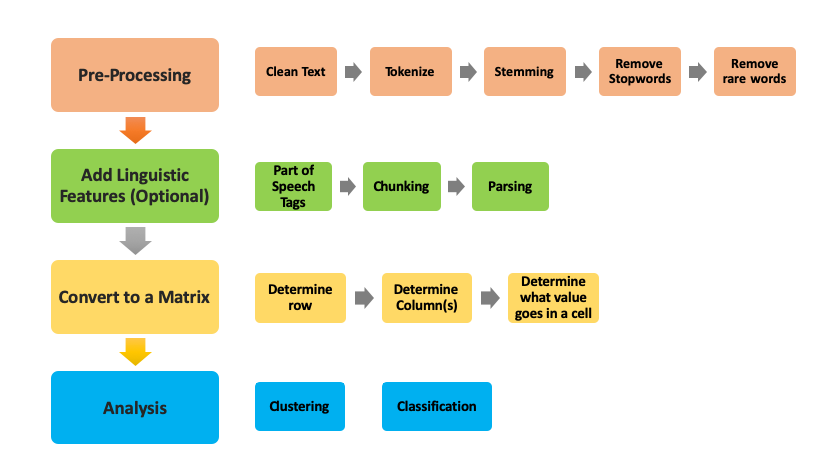
\includegraphics[width=0.9\linewidth]{ChapterText/figures/textanalysispipeline} \end{center}

\subsection{Initial Processing}\label{initial-processing}

The first important step in working with text data is cleaning and
processing.\footnote{Cleaning and processing are discussed extensively
  in Chapter \protect\hyperlink{chap:link}{Record Linkage}.} Textual
data are often messy and unstructured, which makes many researchers and
practitioners overlook their value. Depending on the source, cleaning
and processing these data can require varying amounts of effort but
typically involve a set of established techniques.

\textbf{Tokenization}

The first step in processing text is deciding what terms and phrases are
meaningful. Tokenization separates sentences and terms from each other.
The Natural Language Toolkit (NLTK) (Bird, Klein, and Loper
\protect\hyperlink{ref-bird-09}{2009}) provides simple reference
implementations of standard natural language processing algorithms such
as tokenization---for example, sentences are separated from each other
using punctuation such as period, question mark, or exclamation mark.
However, this does not cover all cases such as quotes, abbreviations, or
informal communication on social media. While separating sentences in a
single language is hard enough, some documents ``code-switch'' (Molina
et al. \protect\hyperlink{ref-molina-16}{2016}), combining multiple
languages in a single document. These complexities are best addressed
through data-driven machine learning frameworks (Kiss and Strunk
\protect\hyperlink{ref-kiss-06}{2006}).

\textbf{Stop words}

Once the tokens are clearly separated, it is possible to perform further
text processing at a more granular, token level. Stop words are a
category of words that have limited semantic meaning (and hence utility)
regardless of the document content. Such words can be prepositions,
articles, common nouns, etc. For example, the word ``the'' accounts for
about 7\% of all words in the Brown Corpus, and ``to'' and ``of'' are
more than 3\% each (Malmkjær \protect\hyperlink{ref-malmkjar-02}{2002}).
We may choose to remove stopwords if we think that they won't be useful
in our analysis. For example, words such as ``the'', ``is'', ``or'' may
not be useful if the task is to classify news articles into the topic of
the article. On the other hand, they may provide information information
if the task is to classify a document into the genre it belongs to or in
identifying the author of the document.

In addition to removing frequent words, it often helps to remove words
that only appear a few times. These words---names, misspellings, or rare
technical terms---are also unlikely to bear significant contextual
meaning. Similar to stop words, these tokens are often disregarded in
further modeling either by the design of the method or by manual removal
from the corpus before the actual analysis.

\textbf{\(N\)-grams}

However, individual words are sometimes not the correct unit of
analysis. For example, blindly removing stop words can obscure important
phrases such as ``systems of innovation,'' ``cease and desist,'' or
``commander in chief.'' Identifying these \(N\)-grams requires looking
for statistical patterns to discover phrases that often appear together
in fixed patterns (Dunning \protect\hyperlink{ref-Dunning-93}{1993}).
These combinations of phrases are often called \emph{collocations}, as
their overall meaning is more than the sum of their parts. N-grams can
be created over any unit of analysis, such as sequences of characters
(called character n-grams) or sequences of phonemes that are used in
speech recognition.

\textbf{Stemming and lemmatization}

Text normalization is another important aspect of preprocessing textual
data. Given the complexity of natural language, words can take multiple
forms dependent on the syntactic structure with limited change of their
original meaning. For example, the word ``system'' morphologically has a
plural ``systems'' or an adjective ``systematic.'' All these words are
semantically similar and---for many tasks---should be treated the same.
For example, if a document has the word ``system'' occurring three
times, ``systems'' once, and ``systematic'' twice, one can assume that
the word ``system'' with similar meaning and morphological structure can
cover all instances and that variance should be reduced to ``system''
with six instances.

The process for text normalization is often implemented using
established lemmatization and stemming algorithms. A \emph{lemma} is the
original dictionary form of a word. For example, ``go,'' ``went,'' and
``goes'' will all have the lemma ``go.'' The stem is a central part of a
given word bearing its primary semantic meaning and uniting a group of
similar lexical units. For example, the words ``order'' and ``ordering''
will have the same stem ``ord.'' Morphy (a lemmatizer provided by the
electronic dictionary WordNet), Lancaster Stemmer, and Snowball Stemmer
are common tools used to derive lemmas and stems for tokens, and all
have implementations in the NLTK (Bird, Klein, and Loper
\protect\hyperlink{ref-bird-09}{2009}).

\subsection{Linguistic Analysis}\label{linguistic-analysis}

So far, we've treated words as tokens without regard to the meaning of
the word or the way it is used, or even what language the word comes
from. There are several techniques in text analysis that are
language-specific that go deeper into the syntax of the document,
paragraph, and sentence structure to extract linguistic characteristics
of the document.

\textbf{Part-of-speech tagging}

When the examples \(x\) are individual words and the labels \(y\)
represent the grammatical function of a word (e.g., whether a word is a
noun, verb, or adjective), the task is called part-of-speech tagging.
This level of analysis can be useful for discovering simple patterns in
text: distinguishing between when ``hit'' is used as a noun (a Hollywood
hit) and when ``hit'' is used as a verb (the car hit the guard rail).

Unlike document classification, the examples \(x\) are not independent:
knowing whether the previous word was an adjective makes it far more
likely that the next word will be a noun than a verb. Thus, the
classification algorithms need to incorporate structure into the
decisions. Two traditional algorithms for this problem are hidden Markov
models (Rabiner \protect\hyperlink{ref-rabiner-89}{1989}) and
conditional random fields (Lafferty, McCallum, and Pereira
\protect\hyperlink{ref-lafferty-01}{2001}), but more complicated models
have higher accuracy (Plank, Søgaard, and Goldberg
\protect\hyperlink{ref-plank-16}{2016}).

\textbf{Order Matters}

All text-processing steps are critical to successful analysis. Some of
them bear more importance than others, depending on the specific
application, research questions, and properties of the corpus. Having
all these tools ready is imperative to producing a clean input for
subsequent modeling and analysis. Some simple rules should be followed
to prevent typical errors. For example, stop words should not be removed
before performing \(n\)-gram indexing, and a stemmer should not be used
where data are complex and require accounting for all possible forms and
meanings of words. Reviewing interim results at every stage of the
process can be helpful.

\subsection{Turning text data into a matrix: How much is a word
worth?}\label{turning-text-data-into-a-matrix-how-much-is-a-word-worth}

The processing stages described above provide us with the columns in our
matrix. Now we have to decide how to assign values in that column for
each word or phrase. In text analysis, we typically refer to them as
tokens (where a token can be a word or a phrase). One simple approach
would be to give each column a binary 0 or 1 value---if this token
occurs in a document, we assign that cell a value of 1 and 0 otherwise.
Another approach would be to assign it the value of how many times this
token occurs in that document (often known as frequency of that term or
token). This is essentially a way to define the importance or value of
this token in this document. Not all words are worth the same; in an
article about sociology, ``social'' may be less important or informative
than ``inequality''. Appropriately weighting\footnote{Term weighting is
  an example of feature engineering discussed in Chapter
  \protect\hyperlink{chap:ml}{Machine Learning}.} and calibrating words
is important for both human and machine consumers of text data: humans
do not want to see ``the'' as the most frequent word of every document
in summaries, and classification algorithms benefit from knowing which
features are actually important to making a decision.

Weighting words requires balancing how often a word appears in a local
context (such as a document) with how much it appears overall in the
document collection. Term frequency--inverse document frequency (TFIDF)
(Salton \protect\hyperlink{ref-salton-68}{1968}) is a weighting scheme
to explicitly balance these factors and prioritize the most meaningful
words. The TFIDF model takes into account both the term frequency of a
given token and its document frequency (Box
\protect\hyperlink{box:text1}{TFIDF}) so that if a highly frequent word
also appears in almost all documents, its meaning for the specific
context of the corpus is negligible. Stop words are a good example when
highly frequent words also bear limited meaning since they appear in
virtually all documents of a given corpus.

\begin{center}\rule{0.5\linewidth}{\linethickness}\end{center}

\textbf{Box: TFIDF}

For every token \(t\) and every document \(d\) in the corpus \(D\) of
size \(\mid D\mid = N\), TFIDF is calculated as
\[tfidf(t,d,D) = tf(t,d) \times
idf(t,D),\] where term frequency is either a simple count,
\[tf(t,d)=f(t,d),\] or a more balanced quantity,
\[tf(t,d) = 0.5+\frac{0.5 \times
  f(t,d)}{\max\{f(t,d):t\in d\}},\] and inverse document frequency is
\[\
idf(t,D) = \log\frac{N}{|\{d\in D:t\in d\}|}.\]

\begin{center}\rule{0.5\linewidth}{\linethickness}\end{center}

\subsection{Analysis}\label{analysis}

Now that we have a matrix with documents as rows, words/phrases as
columns, and let's say the TFIDF score as the value of that word in that
document, we are now ready to run different machine learning methods on
this data. We will not recap all of the methods and evaluation
methodologies already covered in Chapter
\protect\hyperlink{chap:ml}{Machine Learning} here but they can all be
used with text data.

We'll focus on three types of analysis: finding similar documents,
clustering, and classification. For each type of analysis, we`ll focus
on what it allows us to do, what types of tasks social scientists will
find it useful for, and how to evaluate the results of the analysis.

\textbf{Use Case: Finding Similar Documents}

One task social scientists may be interested in is finding similar
documents to a document they're analyzing. This is a routine task during
literature review where we may have a paper and we're interested in
finding similar papers or in disciplines such as law, where lawyers
looking at a case file want to find all prior cases related to the case
being reviewed. The key challenge here is to define what makes two
documents similar - what similarity metrics should we use to calculate
this similarity? Two commonly used metrics are Cosine Similarity and
Kullback--Leibler divergence (Kullback and Leibler
\protect\hyperlink{ref-kullback1951information}{1951}).

Cosine similarity is a popular measure in text analysis. Given two
documents \(d_a\) and \(d_b\), this measure first turns the documents
into vectors (each dimension of the vector can be a word or phrase)
\(\overrightarrow{t_a}\) and \(\overrightarrow{t_b}\), and uses the
cosine similarity (the cosine of the angle between the two vectors) as a
measure of their similarity. This is defined as:

\[SIM_C(\overrightarrow{t_a},\overrightarrow{t_b}) = \frac{\overrightarrow{t_a} \cdot
     \overrightarrow{t_b}}{|\overrightarrow{t_a}|\times|\overrightarrow{t_b}|}.\]

\begin{center}\rule{0.5\linewidth}{\linethickness}\end{center}

Kullback--Leibler (KL) divergence is a measure that allows us to compare
probability distributions in general and is often used to compare two
documents represented as vectors. Given two term vectors
\(\overrightarrow{t_a}\) and \(\overrightarrow{t_b}\), the KL divergence
from vector \(\overrightarrow{t_a}\) to \(\overrightarrow{t_b}\) is
\[D_{KL}(\overrightarrow{t_a}||\overrightarrow{t_b}) =
\sum\limits_{t=1}^m w_{t,a}\times
\log\left(\frac{w_{t,a}}{w_{t,b}}\right),\] where \(w_{t,a}\) and
\(w_{t,b}\) are term weights in the two vectors, respectively, for terms
\(t=1, \ldots, m\).

An averaged KL divergence metric is then defined as
\[D_{AvgKL}(\overrightarrow{t_a}||\overrightarrow{t_b}) = \sum\limits_{t=1}^m (\pi_1\times D(w_{t,a}||w_t)+\pi_2\times D(w_{t,b}||w_t)),\]
where
\(\pi_1 = \frac{w_{t,a}}{w_{t,a}+w_{t,b}}, \pi_2 = \frac{w_{t,b}}{w_{t,a}+w_{t,b}}\),
and \(w_t = \pi_1\times w_{t,a} + \pi_2\times w_{t,b}\) (Huang
\protect\hyperlink{ref-huang-08}{2008}).

A Python-based \texttt{scikit-learn} library provides an implementation
of these measures as well as other machine learning models and
approaches

\textbf{Example: Measuring similarity between documents}

NSF awards are not labeled by scientific field---they are labeled by
program. This administrative classification is not always useful to
assess the effects of certain funding mechanisms on disciplines and
scientific communities. A common need is to understand how awards are
similar to each other even if they were funded by different programs.
Cosine similarity allows us to do just that.

\textbf{Example code}

The Python \texttt{numpy} module is a powerful library of tools for
efficient linear algebra computation. Among other things, it can be used
to compute the cosine similarity of two documents represented by numeric
vectors, as described above. The \texttt{gensim} module that is often
used as a Python-based topic modeling implementation can be used to
produce vector space representations of textual data.

\textbf{Augmenting Similarity Calculations with External Knowledge
repositories}

It's often the case that two, especially short, documents do not have
any words in common but are still similar. In such cases, cosine
similarity or KL divergence do not help us with the similarity
calculations without augmenting the data with additional information.
Often, external data resources that provide relationships between words,
documents, or concepts present in specific domains can be used to
achieve that. Established corpora, such as the Brown Corpus and
Lancaster--Oslo--Bergen Corpus, are one type of such preprocessed
repositories.

Wikipedia and WordNet are examples of another type of lexical and
semantic resources that are dynamic in nature and that can provide a
valuable basis for consistent and salient information retrieval and
clustering. These repositories have the innate hierarchy, or ontology,
of words (and concepts) that are explicitly linked to each other either
by inter-document links (Wikipedia) or by the inherent structure of the
repository (WordNet). In Wikipedia, concepts thus can be considered as
titles of individual Wikipedia pages and the contents of these pages can
be considered as their extended semantic representation.

Information retrieval techniques build on these advantages of WordNet
and Wikipedia. For example, Meij et al.
(\protect\hyperlink{ref-meij-09}{2009}) mapped search queries to the
DBpedia ontology (derived from Wikipedia topics and their
relationships), and found that this mapping enriches the search queries
with additional context and concept relationships. One way of using
these ontologies is to retrieve a predefined list of Wikipedia pages
that would match a specific taxonomy. For example, scientific
disciplines are an established way of tagging documents---some are in
physics, others in chemistry, engineering, or computer science. If a
user retrieves four Wikipedia pages on ``Physics'', ``Chemistry'',
``Engineering'', and ``Computer Science'', they can be further mapped to
a given set of scientific documents to label and classify them, such as
a corpus of award abstracts from the US National Science Foundation.

\emph{Personalized PageRank} is a similarity system that can help with
the task. This system uses WordNet to assess semantic relationships and
relevance between a search query (document \(d\)) and possible results
(the most similar Wikipedia article or articles). This system has been
applied to text categorization (Navigli et al.
\protect\hyperlink{ref-navigli-11}{2011}) by comparing documents to
\emph{semantic model vectors} of Wikipedia pages constructed using
WordNet. These vectors account for the term frequency and their relative
importance given their place in the WordNet hierarchy, so that the
overall \(wiki\) vector is defined as:

\[SMV_{wiki}(s) = \sum\nolimits_{w\in Synonyms(s)} \frac{tf_{wiki}(w)}{|Synsets(w)|}\],

where \(w\) is a token (word) within \(wiki\), \(s\) is a WordNet synset
(a set of synonyms that share a common meaning) that is associated with
every token \(w\) in WordNet hierarchy, \(Synonyms(s)\) is the set of
words (i.e., synonyms) in the synset \(s\), \(tf_{wiki}(w)\) is the term
frequency of the word \(w\) in the Wikipedia article \(wiki\), and
\(Synsets(w)\) is the set of synsets for the word \(w\).

The overall probability of a candidate document \(d\) (e.g., an NSF
award abstract or a PhD dissertation abstract) matching the target
query, or in our case a Wikipedia article \(wiki\), is
\[wiki_{BEST}=\sum\nolimits_{w_t\in d} \max_{s\in Synsets(w_t)} SMV_{wiki}(s),\]
where \(Synsets(w_t)\) is the set of synsets for the word \(w_t\) in the
target document document (e.g., NSF award abstract) and
\(SMV_{wiki}(s)\) is the semantic model vector of a Wikipedia page, as
defined above.

\textbf{Evaluating ``Find Similar'' Methods}

When developing methods to find similar documents, we want to make sure
that we find all relevant documents that are similar to the document
under consideration, and we want to make sure we don't find any
non-relevant documents. Chapter \protect\hyperlink{chap:ml}{Machine
Learning} already touched on the importance of precision and recall for
evaluating the results of machine learning models (Box
\protect\hyperlink{box:text2}{Precision and recall} provides a reminder
of the formulae). The same metrics can be used to evaluate the two goals
we have in finding relevant and similar documents.

\begin{center}\rule{0.5\linewidth}{\linethickness}\end{center}

\textbf{Box: Precision and recall}

Precision computes the type I errors---\emph{false positives} (retrieved
documents that are not relevant)---and is formally defined as
\[\mathrm{Precision} = \frac{|\{\mathrm{relevant\ documents}\}\cap \{\mathrm{retrieved\ documents}\}|}{|\{\mathrm{retrieved\ documents}\}|}.\]
Recall accounts for type II errors---\emph{false negatives} (relevant
documents that were not retrieved)---and is defined as
\[\mathrm{Recall}=\frac{|\{\mathrm{relevant\ documents}\}\cap \{\mathrm{retrieved\ documents}\}|}{|\{\mathrm{relevant\ documents}\}|}.\]

\begin{center}\rule{0.5\linewidth}{\linethickness}\end{center}

We assume that a user has three sets of documents
\(D_a =\{d_{a1},d_{a2},\ldots, d_n\}\),
\(D_b=\{d_{b1}, d_{b2}, \ldots, d_k\}\), and
\(D_c =\{d_{c1},d_{c2},\ldots,d_i\}\). All three sets are clearly tagged
with a disciplinary label: \(D_a\) are computer science documents,
\(D_b\) are physics, and \(D_c\) are chemistry.

The user also has a different set of documents---Wikipedia pages on
``Computer Science,'' ``Chemistry,'' and ``Physics.'' Knowing that all
documents in \(D_a\), \(D_b\), and \(D_c\) have clear disciplinary
assignments, let us map the given Wikipedia pages to all documents
within those three sets. For example, the Wikipedia-based query on
``Computer Science'' should return all computer science documents and
none in physics or chemistry. So, if the query based on the ``Computer
Science'' Wikipedia page returns only 50\% of all computer science
documents, then 50\% of the relevant documents are lost: the recall is
0.5.

On the other hand, if the same ``Computer Science'' query returns 50\%
of all computer science documents but also 20\% of the physics documents
and 50\% of the chemistry documents, then all of the physics and
chemistry documents returned are false positives. Assuming that all
document sets are of equal size, so that \(|D_a| = 10\), \(|D_b|=10\)
and \(|D_c| = 10\), then the precision is \(\frac{5}{12} = 0.42\).

\textbf{\emph{F score}}

The \emph{F score} or \emph{F1 score} combines precision and recall. In
formal terms, the \(F\) score is the harmonic mean of precision and
recall: \[\label{eq:text:F1}
F_1 = 2\cdot \frac{\mathrm{Precision}\cdot \mathrm{Recall}}{\mathrm{Precision}+\mathrm{Recall}}.\]
In terms of type I and type II errors:
\[F_\beta = \frac{(1+\beta^2)\cdot \mathrm{true\ positive}}{(1+\beta^2)\cdot \mathrm{true\ positive} + \beta^2\cdot \mathrm{false\ negative} + \mathrm{false\ positive}},\]
where \(\beta\) is the balance between precision and recall. Thus,
\(F_2\) puts more emphasis on the recall measure and \(F_{0.5}\) puts
more emphasis on precision.

\textbf{Examples}

Some examples from our recent work can demonstrate how Wikipedia-based
labeling and labeled LDA (Ramage et al.
\protect\hyperlink{ref-ramage-09}{2009}; Nguyen et al.
\protect\hyperlink{ref-Nguyen:Boyd-Graber:Resnik:Chang-2014}{2014}) cope
with the task of document classification and labeling in the scientific
domain. See Table \ref{tab:table7-1}.

\begin{longtable}[]{@{}llll@{}}
\caption{\label{tab:table7-1} Wikipedia articles as potential labels
generated by \(n\)-gram indexing of NSF awards}\tabularnewline
\toprule
\begin{minipage}[b]{0.64\columnwidth}\raggedright\strut
\textbf{Abstract excerpt}\strut
\end{minipage} & \begin{minipage}[b]{0.12\columnwidth}\raggedright\strut
\textbf{ProQuest subject category}\strut
\end{minipage} & \begin{minipage}[b]{0.03\columnwidth}\raggedright\strut
\textbf{Labeled LDA}\strut
\end{minipage} & \begin{minipage}[b]{0.09\columnwidth}\raggedright\strut
\textbf{Wikipedia-based labeling}\strut
\end{minipage}\tabularnewline
\midrule
\endfirsthead
\toprule
\begin{minipage}[b]{0.64\columnwidth}\raggedright\strut
\textbf{Abstract excerpt}\strut
\end{minipage} & \begin{minipage}[b]{0.12\columnwidth}\raggedright\strut
\textbf{ProQuest subject category}\strut
\end{minipage} & \begin{minipage}[b]{0.03\columnwidth}\raggedright\strut
\textbf{Labeled LDA}\strut
\end{minipage} & \begin{minipage}[b]{0.09\columnwidth}\raggedright\strut
\textbf{Wikipedia-based labeling}\strut
\end{minipage}\tabularnewline
\midrule
\endhead
\begin{minipage}[t]{0.64\columnwidth}\raggedright\strut
\textbf{Reconfigurable computing platform for smallscale
resource-constrained robot.} Specific applications often require robots
of small size for reasons such as costs, access, and stealth. Smallscale
robots impose constraints on resources such as power or space for
modules\ldots{}\strut
\end{minipage} & \begin{minipage}[t]{0.12\columnwidth}\raggedright\strut
Engineering, Electronics and Electrical; Engineering, Robotics\strut
\end{minipage} & \begin{minipage}[t]{0.03\columnwidth}\raggedright\strut
Motor controller\strut
\end{minipage} & \begin{minipage}[t]{0.09\columnwidth}\raggedright\strut
Robotics, Robot, Fieldprogrammable gate array\strut
\end{minipage}\tabularnewline
\begin{minipage}[t]{0.64\columnwidth}\raggedright\strut
\textbf{Genetic mechanisms of thalamic nuclei specification and the
influence of thalamocortical axons in regulating neocortical area
formation.} Sensory information from the periphery is essential for all
animal species to learn, adapt, and survive in their environment. The
thalamus, a critical structure in the diencephalon, receives sensory
information\ldots{}\strut
\end{minipage} & \begin{minipage}[t]{0.12\columnwidth}\raggedright\strut
Biology, Neurobiology\strut
\end{minipage} & \begin{minipage}[t]{0.03\columnwidth}\raggedright\strut
HSD2 neurons\strut
\end{minipage} & \begin{minipage}[t]{0.09\columnwidth}\raggedright\strut
Sonic hedgehog, Induced stem cell, Nervous system\strut
\end{minipage}\tabularnewline
\begin{minipage}[t]{0.64\columnwidth}\raggedright\strut
\textbf{Poetry 'n acts: The cultural politics of twentieth century
American poets' theater.} This study focuses on the disciplinary blind
spot that obscures the productive overlap between poetry and dramatic
theater and prevents us from seeing the cultural work that this
combination can perform\ldots{}\strut
\end{minipage} & \begin{minipage}[t]{0.12\columnwidth}\raggedright\strut
Literature, American; Theater\strut
\end{minipage} & \begin{minipage}[t]{0.03\columnwidth}\raggedright\strut
Audience\strut
\end{minipage} & \begin{minipage}[t]{0.09\columnwidth}\raggedright\strut
Counterculture of the 1960s, Novel, Modernism\strut
\end{minipage}\tabularnewline
\bottomrule
\end{longtable}

\textbf{Use Case: Clustering}

Another task social scientists often perform is finding themes, topics,
and patterns in a text data set, such as open-ended survey responses,
news articles, or publications. Given open-ended responses from a survey
on how people feel about a certain issue, we may be interested in
finding out the common themes that occur in these responses. Clustering
methods are designed to do exactly that. With text data, clustering is
often used to explore what topics and concepts are present in a new
corpus (collection of documents). It is important to note that if we
already have a pre-specified set of categories and documents that are
tagged with those categories, and the goal is to tag new documents, then
we would use classification methods instead of clustering methods. As we
covered in the previous chapter, clustering a is a form of unsupervised
learning where the goal is exploration and understanding of the data.

As we covered earlier, unsupervised analysis of large text corpora
without extensive investment of time provides additional opportunities
for social scientists and policymakers to gain insights into policy and
research questions through text analysis. The clustering methods
described in the Machine Learning chapter, such as k-means clustering,
can be used for text data as well once the text has been converted to a
matrix as described earlier. We will describe Topic Modeling, that
provides us with another clustering approach specifically designed for
text data.

\subsection{Topic modeling}\label{sec:lda}

Topic modeling is an approach that describes \emph{topics} that
constitute the high-level themes of a text corpus. Topic modeling is
often described as an \emph{information discovery} process: describing
what ``concepts'' are present in a corpus. We refer to them as
``concepts'' or ``topics'' (in quotes) because they typically will be
represented as a probability distribution over the words (that the topic
modeling method groups together) which may or may not be semantically
coherent as a ``topic'' to social scientists.

As topic modeling is a broad subfield of natural language processing and
machine learning, we will restrict our focus to a single method called
Latent Dirichlet Allocation (LDA) (Blei, Ng, and Jordan
\protect\hyperlink{ref-blei-03}{2003}). LDA is a fully Bayesian
extension of probabilistic latent semantic indexing (Hofmann
\protect\hyperlink{ref-hofmann-99}{1999}), itself a probabilistic
extension of latent semantic analysis (Landauer and Dumais
\protect\hyperlink{ref-landauer-97}{1997}). Blei and Lafferty
(\protect\hyperlink{ref-blei-09}{2009}) provide a more detailed
discussion of the history of topic models.

LDA, like all topic models, assumes that there are topics that form the
building blocks of a corpus. Topics are distributions over words and are
often shown as a ranked list of words, with the highest probability
words at the top of the list (see Figure \ref{fig:nyt-topics-3}).
However, we do not know what the topics are a priori; the goal is to
discover what they are (more on this shortly).

\begin{center}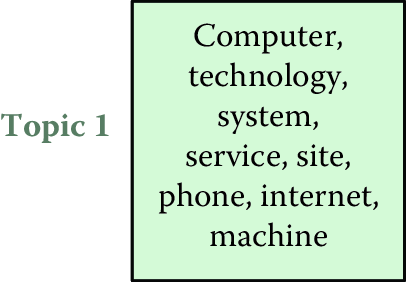
\includegraphics[width=0.5\linewidth]{ChapterText/figures/nyt_topics-1} \end{center}

\begin{center}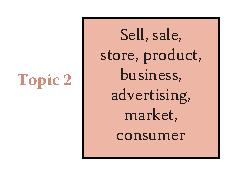
\includegraphics[width=0.5\linewidth]{ChapterText/figures/nyt_topics-2} \end{center}

\begin{figure}

{\centering 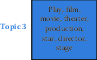
\includegraphics[width=0.5\linewidth]{ChapterText/figures/nyt_topics-3} 

}

\caption{Topics are distributions over words. Here are three example topics learned by latent Dirichlet allocation from a model with 50 topics discovered from the *New York Times* [@sandhaus-08]. Topic 1 appears to be about technology, Topic 2 about business, and Topic 3 about the arts}\label{fig:nyt-topics-3}
\end{figure}

In addition to assuming that there exist some number of topics that
explain a corpus, LDA also assumes that each document in a corpus can be
explained by a small number of topics. For example, taking the example
topics from Figure \ref{fig:nyt-topics-3}, a document titled ``Red
Light, Green Light: A Two-Tone LED to Simplify Screens'' would be about
Topic 1, which appears to be about technology. However, a document like
``Forget the Bootleg, Just Download the Movie Legally'' would require
all three of the topics. The set of topics that are used by a document
is called the document's \emph{allocation} (Figure
\ref{fig:nyt-documents}). This terminology explains the name
\emph{latent Dirichlet allocation}: each document has an allocation over
latent topics governed by a Dirichlet distribution.

\begin{figure}

{\centering 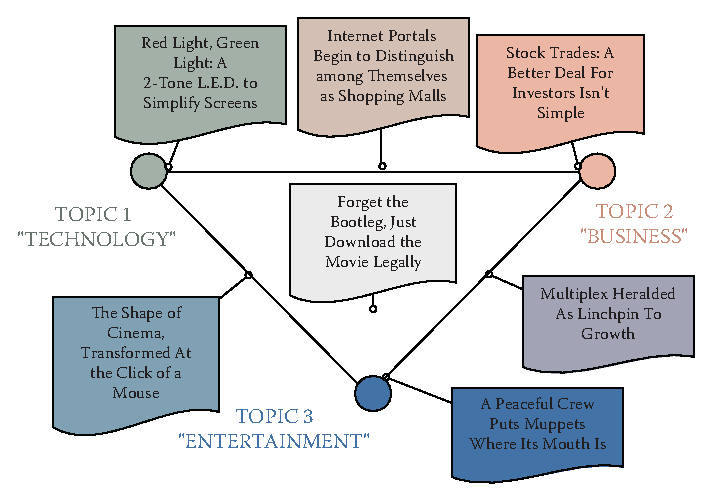
\includegraphics[width=0.7\linewidth]{ChapterText/figures/nyt_documents} 

}

\caption{Allocations of documents to topics}\label{fig:nyt-documents}
\end{figure}

\subsubsection{\texorpdfstring{Inferring ``topics'' from raw
text}{Inferring topics from raw text}}\label{inferring-topics-from-raw-text}

Algorithmically, the problem can be viewed as: Given a corpus and an
integer \(k\) as input, provide the \(k\) topics that best describe the
document collection: a process called \emph{posterior inference}. The
most common algorithm for solving this problem is a technique called
\emph{Gibbs sampling} (Geman and Geman
\protect\hyperlink{ref-geman-90}{1990}).

Gibbs sampling works at the word level to discover the topics that best
describe a document collection. Each word is associated with a single
topic, explaining why that word appeared in a document. For example,
consider the sentence ``Hollywood studios are preparing to let people
download and buy electronic copies of movies over the Internet.''. Each
word in this sentence is associated with a topic: ``Hollywood'' might be
associated with an arts topic; ``buy'' with a business topic; and
``Internet'' with a technology topic (Figure \ref{fig:inference-1}).

\begin{figure}

{\centering 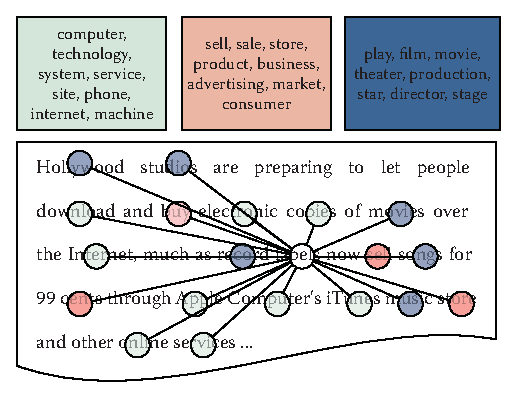
\includegraphics[width=0.7\linewidth]{ChapterText/figures/inference_1} 

}

\caption{Each word is associated with a topic. Gibbs sampling inference iteratively resamples the topic assignments for each word to discover the most likely topic assignments that explain the document collection}\label{fig:inference-1}
\end{figure}

This is where we should eventually get. However, we do not know this to
start. So, we can initially assign words to topics randomly. This will
result in poor topics, but we can make those topics better. We improve
these topics by taking each word, pretending that we do not know the
topic, and selecting a new topic for the word.

A topic model wants to do two things: it does not want to use many
topics in a document, and it does not want to use many words in a topic.
So the algorithm will keep track of how many times a document \(d\) has
used a topic \(k\), \(N_{d,k}\), and how many times a topic \(k\) has
used a word \(w\), \(V_{k,w}\). For notational convenience, it will also
be useful to keep track of marginal counts of how many words are in a
document, \[N_{d, \cdot} \equiv \sum_k N_{d,k},\] and how many words are
associated with a topic, \[V_{k, \cdot} \equiv \sum_w V_{k, w}.\] The
algorithm removes the counts for a word from \(N_{d,k}\) and \(V_{k,w}\)
and then changes the topic of a word (hopefully to a better topic than
the one it had before). Through many thousands of iterations of this
process, the algorithm can find topics that are coherent, useful, and
characterize the data well.

The two goals of topic modeling---balancing document allocations to
topics and topics' distribution over words---come together in an
equation that multiplies them together. A good topic will be both common
in a document and explain a word's appearance well.

\begin{center}\rule{0.5\linewidth}{\linethickness}\end{center}

\textbf{Example: Gibbs sampling for topic models}

The topic assignment \(z_{d,n}\) of word \(n\) in document \(d\) is
proportional to
\[p(z_{d,n}=k) \propto \left( \underset{\text{how much doc likes the topic}}{\frac{N_{d,k} + \alpha}{N_{d, \cdot} + K \alpha}} \right) \left(\underset{\text{how much topic likes the word}}{\frac{V_{k,w_{d,n}} + \beta}{V_{k, \cdot} + V \beta}} \right),\]
where \(\alpha\) and \(\beta\) are smoothing factors that prevent a
topic from having zero probability if a topic does not use a word or a
document does not use a topic (Wallach, Mimno, and McCallum
\protect\hyperlink{ref-wallach-09b}{2009}). Recall that we do not
include the token that we are sampling in the counts for \(N\) or \(V\).

For the sake of concreteness, assume that we have three documents with
the following topic assignments:

\begin{itemize}
\item
  Document 1: \(^A\)dog\(_3\) \(^B\)cat\(_2\) \(^C\)cat\(_3\)
  \(^D\)pig\(_1\)
\item
  Document 2: \(^E\)hamburger\(_2\) \(^F\)dog\(_3\)
  \(^G\)hamburger\(_1\)
\item
  Document 3: \(^H\)iron\(_1\) \(^I\)iron\(_3\) \(^J\)pig\(_2\)
  \(^K\)iron\(_2\)
\end{itemize}

If we want to sample token B (the first instance of of ``cat'' in
document 1), we compute the conditional probability for each of the
three topics (\(z=1,2,3\)): \[\begin{aligned}
p(z_B = 1) = & \frac{1 + 1.000}{3 + 3.000} \times \frac{0
    + 1.000}{3 + 5.000} = 0.333 \times 0.125 = 0.042, \\[4pt]
p(z_B = 2) = & \frac{0 + 1.000}{3 + 3.000} \times \frac{0
    + 1.000}{3 + 5.000} = 0.167 \times 0.125 = 0.021\mbox{, and} \\[4pt]
p(z_B = 3) = & \frac{2 + 1.000}{3 + 3.000} \times \frac{1 + 1.000}{4 + 5.000} = 0.500 \times 0.222 = 0.111.\end{aligned}\]
To reiterate, we do not include token B in these counts: in computing
these conditional probabilities, we consider topic 2 as never appearing
in the document and ``cat'' as never appearing in topic 2. However,
``cat'' does appear in topic 3 (token C), so it has a higher probability
than the other topics. After renormalizing, our conditional
probabilities are \((0.24, 0.12, 0.64)\). We then sample the new
assignment of token B to be topic 3 two times out of three. Griffiths
and Steyvers (\protect\hyperlink{ref-griffiths-04}{2004}) provide more
details on the derivation of this equation.

\subsubsection{Applications of topic
models}\label{applications-of-topic-models}

Topic modeling is most often used for topic exploration, allowing users
to understand the contents of large text corpora. Thus, topic models
have been used, for example, to understand what the National Institutes
of Health funds (Talley, Newman, Mimno, Herr II, et al.
\protect\hyperlink{ref-talley2011database}{2011}); to compare and
contrast what was discussed in the North and South in the Civil War
(Nelson \protect\hyperlink{ref-nelson-10}{2010}); and to understand how
individuals code in large programming projects (Maskeri, Sarkar, and
Heafield \protect\hyperlink{ref-maskeri-08}{2008}).

Topic models can also be used as features to more elaborate algorithms
such as machine translation (Hu et al.
\protect\hyperlink{ref-Hu:Zhai:Eidelman:Boyd-Graber-2014}{2014}),
detecting objects in images (Wang, Blei, and Fei-Fei
\protect\hyperlink{ref-wang-09b}{2009}), or identifying political
polarization (Paul and Girju \protect\hyperlink{ref-paul-10}{2010}).
Boyd-Graber, Hu, and Mimno
(\protect\hyperlink{ref-boyd-graber-17}{2017}) summarize applications of
topic models in the humanities, information retrieval, and social
sciences.

Blei and McAuliffe (\protect\hyperlink{ref-blei-07b}{2007}) apply topic
models to classification and regression tasks such as sentiment
analysis. As discussed in the previous chapter, such methods require a
feature-based representation of the data. An advantage of using topic
models is that the distribution over topics itself can serve as a
feature.

For example, to predict whether a legislator will vote on a bill,
Gerrish and Blei (\protect\hyperlink{ref-gerrish-12}{2012}) learn a
topic model that encodes each bill (proposed piece of legislation) as a
vector. To predict how a legislator will vote on a bill, the model takes
a dot product between the bill's distribution over topics and a
legislator's ideology vector. The higher score, the more compatible they
are and the more likely the legislator is to vote on the bill.
Conversely, the lower the score, the less likely it is the legislator
will vote on the bill.

This formulation should remind you of logistic regression; however, the
features are learned automatically rather than the feature engineering
approach described in the last chapter.

\textbf{Use Case: Document classification}

The section above focused on the task of finding topics and themes in a
new text data set. In many cases, we already know a set of topics---this
could be the set of topics or research fields as described by the Social
Science Research Network or the set of sections (local news,
international, sports, finance, etc.) in a news publication. The task we
often face is to automatically categorize new documents into an existing
set of categories. In text analysis, this is called text classification
or categorization and uses supervised learning techniques from machine
learning described in the earlier chapter.

Text classification typically requires two things: a set of categories
we want documents to be categorized into (each document can belong to
one or more categories) and a set of documents annotated/tagged with one
or more categories from step 1.

For example, if we want to classify Twitter or Facebook posts as being
about health or finance, a classification method would take a small
number of posts, manually tagged as belonging to either health or
finance, and train a classification model. This model can then be used
to automatically classify new posts as belonging to either health or
finance.

All of the classification (supervised learning) methods we covered in
the Machine Learning chapter can be used here once the text data has
been processed and converted to a matrix. Neural Networks (Iyyer et al.
\protect\hyperlink{ref-iyyer-15}{2015}), Naive Bayes (Lewis
\protect\hyperlink{ref-lewis-05}{1998}), and Support Vector Machines
(Zhu et al. \protect\hyperlink{ref-zhu-13}{2013}) are some of the
commonly used methods applied to text data.

\begin{center}\rule{0.5\linewidth}{\linethickness}\end{center}

\textbf{Example: Using text to categorize scientific fields}

The National Center for Science and Engineering Statistics, the US
statistical agency charged with collecting statistics on science and
engineering, uses a rule-based system to manually create categories of
science; these are then used to categorize research as ``physics'' or
``economics'' (Mortensen and Bloch
\protect\hyperlink{ref-oecd2005measurement}{2005}; Economic Co-operation
and Development \protect\hyperlink{ref-manual2004summary}{2004}). In a
rule-based system there is no ready response to the question ``how much
do we spend on climate change, food safety, or biofuels?'' because
existing rules have not created such categories. Text analysis
techniques can be used to provide such detail without manual collation.
For example, data about research awards from public sources and about
people funded on research grants from UMETRICS can be linked with data
about their subsequent publications and related student dissertations
from ProQuest. Both award and dissertation data are text documents that
can be used to characterize what research has been done, provide
information about which projects are similar within or across
institutions, and potentially identify new fields of study (Talley,
Newman, Mimno, Herr II, et al.
\protect\hyperlink{ref-talley2011database}{2011}).

\textbf{Applications}

\textbf{Spam Detection}

One simple but ubiquitous example of document classification is spam
detection: an email is either an unwanted advertisement (spam) or it is
not. Document classification techniques such as naïve Bayes (Lewis
\protect\hyperlink{ref-lewis-05}{1998}) touch essentially every email
sent worldwide, making email usable even though most emails are spam.

\textbf{Sentiment analysis}

Instead of being what a document is about, a label \(y\) could also
reveal the speaker. A recent subfield of natural language processing is
to use machine learning to reveal the internal state of speakers based
on what they say about a subject (Pang and Lee
\protect\hyperlink{ref-pang-08}{2008}). For example, given an example of
sentence \(x\), can we determine whether the speaker is a Liberal or a
Conservative? Is the speaker happy or sad?

Simple approaches use dictionaries and word counting methods (Pennebaker
and Francis \protect\hyperlink{ref-pennebaker-99}{1999}), but more
nuanced approaches make use of \emph{domain}-specific information to
make better predictions. One uses different approaches to praise a
toaster than to praise an air conditioner (Blitzer, Dredze, and Pereira
\protect\hyperlink{ref-blitzer-07}{2007}); Liberals and Conservatives
each frame health care differently from how they frame energy policy
(Nguyen, Boyd-Graber, and Resnik
\protect\hyperlink{ref-nguyen-13:shlda}{2013}).

\textbf{Evaluating Text Classification Methods}

The metrics used to evaluate text classification methods are the same as
those used in supervised learning, as described in the Machine Learning
chapter. The most commonly used metrics include accuracy, precision,
recall, AUC, and F1 score.

\section{Word Embeddings and Deep
Learning}\label{word-embeddings-and-deep-learning}

In discussing topic models, we learned a vector that summarized the
content of each document. This is useful for applications where you can
use a single, short vector to summarize a document for a downstream
machine learning application. However, modern research doesn't stop
there, it learns vector representations of everything from documents
down to sentences and words.

First, let's consider this from a high-level perspective. The goal of
representation learning (Bengio, Courville, and Vincent
\protect\hyperlink{ref-bengio-13}{2013}) is to take an input and
transform it into a vector that computers can understand. Similar inputs
should be close together in vector space. E.g., ``dog'' and ``poodle''
should have similar vectors, while ``dog'' and ``chainsaw'' should not.

A well-known technique for word representation is word2vec (Mikolov et
al. \protect\hyperlink{ref-mikolov-13}{2013}). Using an objective
function similar to logistic regression, it predicts, given a word,
whether another word will appear in the same context. For example, the
dot product for ``dog'' and ``pet'', ``dog'' and ``leash'', and ``dog''
and ``wag'' will be high but those for ``dog'' and ``rectitude'',
``dog'' and ``examine'', and ``dog'' and ``cloudy'' will be lower.
Training a model to do this for all of the words in English will produce
vector representations for ``dog'' and ``poodle'' that are quite close
together.

This model has been well adopted throughout natural language processing
(Ward \protect\hyperlink{ref-church-17}{2017}). Downloading word2vec
vectors for words and using them as features in your machine learning
pipeline (e.g., for document classification by averaging the words in
the document) will likely improve a supervised classification task.

But word representations are not the end of the story. A word only makes
sense in the context of the sentence in which it appears: e.g., ``I
deposited my check at the bank'' versus ``The airplane went into a bank
of clouds''. A single word per vector does not capture these subtle
effects. More recent models named after Muppets (long, uninteresting
story) tries to capture broader relationships between words within
sentences to create \emph{contextualized representations}.

ELMO (Peters et al. \protect\hyperlink{ref-peters-18}{2018}) and BERT
(Devlin et al. \protect\hyperlink{ref-devlin-18}{2019}) both use deep
learning to take word vectors (a la word2vec) to create representations
that make sense given a word's \emph{context}. These are also useful
features to use in supervised machine learning contexts if higher
accuracy is your goal.

However, these techniques are not always the best tools for social
scientists. They are not always interpretable---it is often hard to tell
why you got the answer you did (Ribeiro, Singh, and Guestrin
\protect\hyperlink{ref-ribeiro-16}{2016}), and slightly changing the
input the models can dramatically change the results (Feng et al.
\protect\hyperlink{ref-feng-18}{2018}). Given that our goal is often
understanding our data, it is probably better to start first with the
simpler (and faster methods) mentioned here to understand your data
first.

\section{Text analysis tools}\label{text-analysis-tools}

We are fortunate to have access to a set of powerful open source text
analysis tools. We describe three here.

\textbf{The Natural Language Toolkit}

The NLTK is a commonly used natural language toolkit that provides a
large number of relevant solutions for text analysis. It is Python-based
and can be easily integrated into data processing and analytical scripts
by a simple \texttt{import\ nltk} (or similar for any one of its
submodules).

The NLTK includes a set of tokenizers, stemmers, lemmatizers and other
natural language processing tools typically applied in text analysis and
machine learning. For example, a user can extract tokens from a document
\emph{doc} by running the command
\texttt{tokens\ =\ nltk.word\_tokenize(doc)}.

Useful text corpora are also present in the NLTK distribution. For
example, the stop words list can be retrieved by running the command
\texttt{stops\ =\ nltk.corpus.stopwords.words(language)}. These stop
words are available for several languages within NTLK, including
English, French, and Spanish.

Similarly, the Brown Corpus or WordNet can be called by running
\texttt{from\ nltk.corpus\ import\ wordnet/brown}. After the corpora are
loaded, their various properties can be explored and used in text
analysis; for example,
\texttt{dogsyn\ =\ wordnet.synsets(\textquotesingle{}dog\textquotesingle{})}
will return a list of WordNet synsets related to the word ``dog.''

Term frequency distribution and \(n\)-gram indexing are other techniques
implemented in NLTK. For example, a user can compute frequency
distribution of individual terms within a document \emph{doc} by running
a command in Python: \texttt{fdist\ =\ nltk.FreqDist(text)}. This
command returns a dictionary of all tokens with associated frequency
within \emph{doc}.

\(N\)-gram indexing is implemented as a chain-linked collocations
algorithm that takes into account the probability of any given two,
three, or more words appearing together in the entire corpus. In
general, \(n\)-grams can be discovered as easily as running
\texttt{bigrams\ =\ nltk.bigrams(text)}. However, a more sophisticated
approach is needed to discover statistically significant word
collocations, as we show in Listing
\protect\hyperlink{list:text1}{Bigrams}.

Bird, Klein, and Loper (\protect\hyperlink{ref-bird-09}{2009}) provide a
detailed description of NLTK tools and techniques. See also the official
NLTK website.\footnote{\url{http://www.nltk.org}}

\begin{Shaded}
\begin{Highlighting}[]
\NormalTok{def }\KeywordTok{bigram_finder}\NormalTok{(texts)}\OperatorTok{:}
\StringTok{  }\CommentTok{# NLTK bigrams from a corpus of documents separated by new line}
\StringTok{  }\NormalTok{tokens_list =}\StringTok{ }\KeywordTok{nltk.word_tokenize}\NormalTok{(}\KeywordTok{re.sub}\NormalTok{(}\StringTok{"}\CharTok{\textbackslash{}n}\StringTok{"}\NormalTok{,}\StringTok{" "}\NormalTok{,texts))}
\NormalTok{  bgm    =}\StringTok{ }\KeywordTok{nltk.collocations.BigramAssocMeasures}\NormalTok{()}
\NormalTok{  finder =}\StringTok{ }\KeywordTok{nltk.collocations.BigramCollocationFinder.from_words}\NormalTok{(tokens_list)}
\NormalTok{  scored =}\StringTok{ }\KeywordTok{finder.score_ngrams}\NormalTok{( bgm.likelihood_ratio  )}

  \CommentTok{# Group bigrams by first word in bigram.}
\NormalTok{  prefix_keys =}\StringTok{ }\KeywordTok{collections.defaultdict}\NormalTok{(list)}
  \ControlFlowTok{for}\NormalTok{ key, scores }\ControlFlowTok{in}\NormalTok{ scored}\OperatorTok{:}
\StringTok{      }\NormalTok{prefix_keys[key[}\DecValTok{0}\NormalTok{]]}\KeywordTok{.append}\NormalTok{((key[}\DecValTok{1}\NormalTok{], scores))}

  \CommentTok{# Sort keyed bigrams by strongest association.}
  \ControlFlowTok{for}\NormalTok{ key }\ControlFlowTok{in}\NormalTok{ prefix_keys}\OperatorTok{:}
\StringTok{      }\NormalTok{prefix_keys[key]}\KeywordTok{.sort}\NormalTok{(}\DataTypeTok{key =}\NormalTok{ lambda x}\OperatorTok{:}\StringTok{ }\OperatorTok{-}\NormalTok{x[}\DecValTok{1}\NormalTok{])}
\end{Highlighting}
\end{Shaded}

Listing: Python code to find bigrams using NLTK

\textbf{Stanford CoreNLP}

While NLTK's emphasis is on simple reference implementations, Stanford's
CoreNLP (Manning et al.
\protect\hyperlink{ref-manning2014stanford}{2014}) is focused on fast
implementations of cutting-edge algorithms, particularly for syntactic
analysis (e.g., determining the subject of a sentence).\footnote{\url{https://stanfordnlp.github.io/CoreNLP/}}

\textbf{MALLET}

For probabilistic models of text, MALLET, the MAchine Learning for
LanguagE Toolkit (McCallum \protect\hyperlink{ref-mallet}{2002}), often
strikes the right balance between usefulness and usability. It is
written to be fast and efficient but with enough documentation and easy
enough interfaces to be used by novices. It offers fast, popular
implementations of conditional random fields (for part-of-speech
tagging), text classification, and topic modeling.

\textbf{Spacy.io}

While NLTK is optimized for teaching NLP concepts to students, Spacy.io
{[}\url{http://spacy.io}{]} is optimized for practical application. It
is fast, contains many models for well-trodden tasks (classification,
parsing, finding entities in sentences, etc.). It also has pre-trained
models (including word and sentence representations) that can help
practicioners quickly build competitive models.

\textbf{Pytorch}

For the truly adventurous who want to build their own deep learning
models for text, PyTorch {[}\url{http://pytorch.org}{]} offers the
flexibility to go from word vectors to complete deep representations of
sentences.

\section{Summary}\label{summary-5}

Many of the new sources of data that are of interest to social
scientists is text: tweets, Facebook posts, corporate emails, and the
news of the day. However, the meaning of these documents is buried
beneath the ambiguities and noisiness of the informal, inconsistent ways
by which humans communicate with each other and traditional data
analysis methods do not work with text data directly. Despite attempts
to formalize the meaning of text data through asking users to tag
people, apply metadata, or to create structured representations, these
attempts to manually curate meaning are often incomplete, inconsistent,
or both.

These aspects make text data difficult to work with, but also a
rewarding object of study. Unlocking the meaning of a piece of text
helps bring machines closer to human-level intelligence---as language is
one of the most quintessentially human activities---and helps overloaded
information professionals do their jobs more effectively: understand
large corpora, find the right documents, or automate repetitive tasks.
And as an added bonus, the better computers become at understanding
natural language, the easier it is for information professionals to
communicate their needs: one day using computers to grapple with big
data may be as natural as sitting down for a conversation over coffee
with a knowledgeable, trusted friend.

\section{Resources}\label{resources-3}

Text analysis is one of the more complex tasks in big data analysis.
Because it is unstructured, text (and natural language overall) requires
significant processing and cleaning before we can engage in interesting
analysis and learning. In this chapter we have referenced several
resources that can be helpful in mastering text mining techniques:

\begin{itemize}
\item
  The Natural Language Toolkit is one of the most popular Python-based
  tools for natural language processing. It has a variety of methods and
  examples that are easily accessible online.\footnote{\url{http://www.nltk.org}}
  The book by Bird, Klein, and Loper
  (\protect\hyperlink{ref-bird-09}{2009}), available online, contains
  multiple examples and tips on how to use NLTK. This is a great package
  to use if you want to \emph{understand} these models.
\item
  A paper by Anna Huang (\protect\hyperlink{ref-huang-08}{2008})
  provides a brief overview of the key similarity measures for text
  document clustering discussed in this chapter, including their
  strengths and weaknesses in different contexts.
\item
  Materials at the MALLET website (McCallum
  \protect\hyperlink{ref-mallet}{2002}) can be specialized for the
  unprepared reader but are helpful when looking for specific solutions
  with topic modeling and machine classification using this toolkit.
\item
  We provide an example of how to run topic modeling using MALLET on
  textual data from the National Science Foundation and Norwegian
  Research Council award abstracts.\footnote{\url{http://www.umiacs.umd.edu/~jbg/lda_demo}}
\item
  If you do not care about understanding and just want models that are
  easy to use and fast, spaCy {[}\url{https://spacy.io/}{]} has a useful
  minimal core of models for the average user. spaCy is the most useful
  toolkit for the preprocessing steps of dataset preparation.
\item
  For more advanced models (classification, tagging, etc.), the AllenNLP
  toolkit {[}\url{https://allennlp.org/}{]} is useful if you want to run
  state of the art models and tweak them just slightly.
\item
  Text corpora: A set of multiple similar documents is called a
  \emph{corpus}. For\\
  example, the Brown University Standard Corpus of Present-Day American
  English, or just the Brown Corpus (Francis and Kucera
  \protect\hyperlink{ref-browncorpus}{1979}), is a collection of
  processed documents from works published in the United States in 1961.
  The Brown Corpus was a historical milestone: it was a machine-readable
  collection of a million words across 15 balanced genres with each word
  tagged with its part of speech (e.g., noun, verb, preposition). The
  British National Corpus (University of Oxford
  \protect\hyperlink{ref-bnc}{2006}) repeated the same process for
  British English at a larger scale. The Penn Treebank (Marcus,
  Santorini, and Marcinkiewicz \protect\hyperlink{ref-marcus-93}{1993})
  provides additional information: in addition to part-of-speech
  annotation, it provides \emph{syntactic} annotation. For example, what
  is the object of the sentence ``The man bought the hat''? These
  standard corpora serve as training data to train the classifiers and
  machine learning techniques to automatically analyze text (Halevy,
  Norvig, and Pereira \protect\hyperlink{ref-halevy-09}{2009}).
\item
  The \emph{Text Analysis} workbook of Chapter
  \protect\hyperlink{chap:workbooks}{Workbooks} provides an introduction
  to topic modeling with Python.\footnote{See
    \url{https://workbooks.coleridgeinitiative.org}.}
\end{itemize}

\hypertarget{chap:networks}{\chapter{Networks: The
Basics}\label{chap:networks}}

\textbf{Jason Owen-Smith}

Social scientists are typically interested in describing the activities
of individuals and organizations (such as households and firms) in a
variety of economic and social contexts. The frame within which data has
been collected will typically have been generated from tax or other
programmatic sources. The new types of data permit new units of
analysis---particularly network analysis---largely enabled by advances
in mathematical graph theory. This chapter provides an overview of how
social scientists can use network theory to generate measurable
representations of patterns of relationships connecting entities. The
value of the new framework is not only in constructing different
right-hand-side variables but also in studying an entirely new unit of
analysis that lies somewhere between the largely atomistic actors that
occupy the markets of neo-classical theory and the tightly managed
hierarchies that are the traditional object of inquiry of sociologists
and organizational theorists.

\section{Introduction}\label{introduction-3}

Social Scientists have studied networks for a long time. A lot of the
theory behind network analysis in fact comes from the social sciences
where we studied relationships between people, groups, and organizations
(Moreno and Jennings \protect\hyperlink{ref-moreno1934}{1934}). What's
different today is the scale of the data available to us to perform this
analysis. Instead of studying a group of 25 participants in a karate
club (Zachary \protect\hyperlink{ref-zachary1977}{1977}), we now have
data about hundreds of millions of people communicating with each other
through social media channels, or hundreds of thousands of employees in
a large multinational organizations collaborating on projects. This
increased scale requires us to explore new methods of answering the same
questions that we used to be interested in, as well as opens up avenues
to answer new questions that could not be answered before.\footnote{If
  you have examples from your own research using the methods we describe
  in this chapter, please submit a link to the paper (and/or code) here:
  \url{https://textbook.coleridgeinitiative.org/submitexamples}}

\begin{center}\rule{0.5\linewidth}{\linethickness}\end{center}

\textbf{Box: Network Analysis Examples}

\begin{itemize}
\item
  \textbf{Example 1: Cascading Information}\footnote{\url{https://cs.stanford.edu/people/jure/pubs/recurrence-www16.pdf}}
  (Ugander et al. \protect\hyperlink{ref-ugander2011}{2011}). By using
  network analysis, researchers were able to characterize how
  information travels and recurs in patterns, exhibiting multiple bursts
  of popularity.
\item
  \textbf{Example 2: Large-Scale Social Networks}\footnote{\url{https://www.ncbi.nlm.nih.gov/pmc/articles/PMC4000208}}
  (Stopczynski et al. \protect\hyperlink{ref-stopczynski2014}{2014}).
  Using data from a variety of sources to determine how people are
  connected, Stopczynski et al. are able to observe how communities form
  and social interactions change over time.
\item
  \textbf{Example 3: Facebook Social Graph}\footnote{\url{http://snap.stanford.edu/class/cs224w-readings/backstrom12fb.pdf}}
  (Cheng et al. \protect\hyperlink{ref-cheng2016}{2016}). A study of the
  Facebook friendship network was able to characterize how connected
  people were on the social networking site. By studying clustering and
  friendship preferences, the researchers were able to see how
  communities form and explore the ``six degrees of separation''
  phenomenon on Facebook.
\end{itemize}

\begin{center}\rule{0.5\linewidth}{\linethickness}\end{center}

This chapter provides a basic introduction to the analysis of large
networks for social science research and practice. We describe how to
use data from existing social networks as well as how to turn
``non-network'' data into a network to perform further analysis. We then
describe different measures that can be calculated to understand the
properties of the network being analyzed, show different network
visualization techniques, and discuss social science questions that
these network measures and visualizations can help us answer.

We use the comparison of the collaboration networks of two
research-intensive universities to show how to perform network analysis
but the same approach generalizes to other types of problems. The
collaboration networks and a grant co-employment network for a large
public university examined in this chapter are derived from data
produced by the multi-university Committee on Institutional Cooperation
(CIC)'s UMETRICS project (Lane et al.
\protect\hyperlink{ref-lane2015new}{2015}). The snippets of code that
are provided are from the \texttt{igraph} package for network analysis
as implemented in Python.

\section{What are networks?}\label{what-are-networks}

Networks are measurable representations of relationships connecting
entities. What this means is that there are two fundamental questions to
ask of any network representation: First, what are the nodes, or
entities that are connected? Second, what are the relationships (ties or
edges) connecting the nodes? Once we have the representation, we can
then analyze the underlying data and relationships through the measures
and methods described in this chapter. This is of great interest because
a great deal of research in social sciences demonstrates that networks
are essential to understanding behaviors and outcomes at both the
individual and the organizational level.

Networks offer not just another convenient set of right-hand-side
variables, but an entirely new unit of analysis that lies somewhere
between the largely atomistic actors that occupy the markets of
neo-classical theory and the tightly managed hierarchies that are the
traditional object of inquiry of sociologists and organizational
theorists. As Walter W. Powell
(\protect\hyperlink{ref-powell2003neither}{2003}) puts it in a
description of buyer supplier networks of small Italian firms: ``when
the entangling of obligation and reputation reaches a point where the
actions of the parties are interdependent, but there is no common
ownership or legal framework \ldots{} such a transaction is neither a
market exchange nor a hierarchical governance structure, but a separate,
different mode of exchange.''

Existing as they do between the uncoordinated actions of independent
individuals and coordinated work of organizations, networks offer a
unique level of analysis for the study of scientific and creative teams
(Wuchty, Jones, and Uzzi
\protect\hyperlink{ref-wuchty2007increasing}{2007}), collaborations
(Kabo et al. \protect\hyperlink{ref-kabo2015shared}{2015}), and clusters
of entrepreneurial firms (Owen-Smith and Powell
\protect\hyperlink{ref-owen2004knowledge}{2004}).

The following sections will introduce you to this approach to studying
innovation and discovery, focusing on examples drawn from
high-technology industries and particularly from the scientific
collaborations among grant-employed researchers at UMETRICS
universities. We make particular use of a network that connects
individual researchers to grants that paid their salaries in 2012 for a
large public university. The grants network for university A includes
information on 9,206 individuals who were employed on 3,389 research
grants from federal science agencies in a single year. The web of
partnerships that emerges from university scientists' decentralized
efforts to build effective collaborations and teams generates a
distinctive social infrastructure for cutting-edge science.

While this chapter focuses on social networks, the techniques described
here have been used to examine the structure of networks such as the
World Wide Web, the national railway route map of the USA, the food web
of an ecosystem, or the neuronal network of a particular species of
animal.

\section{Structure for this chapter}\label{structure-for-this-chapter}

The chapter first introduces the most common structures for large
network data, briefly introduce three key social ``mechanisms of
action'' by which social networks are thought to have their effects, and
then present a series of basic measures that can be used to quantify
characteristics of entire networks and the relative position individual
people or organizations hold in the differentiated social structure
created by networks.

Taken together, these measures offer an excellent starting point for
examining how global network structures create opportunities and
challenges for the people in them, for comparing and explaining the
productivity of collaborations and teams, and for making sense of the
differences between organizations, industries, and markets that hinge on
the pattern of relationships connecting their participants.

Understanding the productivity and effects of university research thus
requires an effort to measure and characterize the networks on which it
depends. As suggested, those networks influence outcomes in three ways:
first, they distinguish among individuals; second, they differentiate
among teams; and third, they help to distinguish among
research-performing universities. Most research-intensive institutions
have departments and programs that cover similar arrays of topics and
areas of study. What distinguishes them from one another is not the
topics they cover but the ways in which their distinctive collaboration
networks lead them to have quite different scientific capabilities.

\section{Turning Data into a Network}\label{turning-data-into-a-network}

Networks are comprised of \emph{nodes}, which represent entities that
can be connected to one another, and of ties that represent the
relationships connecting nodes. When ties are undirected (representing a
relationshop between the nodes that is not directional) they are called
\emph{edges}. When they are directed (as when I lend money to you and
you do or do not reciprocate) they are called \emph{arcs}. Nodes, edges
and arcs can, in principle, be anything: patents and citations, web
pages and hypertext links, scientists and collaborations, teenagers and
intimate relationships, nations and international trade agreements. The
very flexibility of network approaches means that the first step toward
doing a network analysis is to first turn our data into a graph by
clearly defining what counts as a node and what counts as a tie. In
traditional social network analysis studies, there is a natural
representation of the data as a network. People are often nodes, and
some type of communication between them form the ``ties''. While this
seems like an easy move, it often requires deep thought. For instance,
an interest in innovation and discovery could take several forms. We
could be interested in how universities differ in their capacity to
respond to new requests for proposals (a macro question that would
require the comparison of full networks across campuses). We could
wonder what sorts of training arrangements lead to the best outcomes for
graduate students (a more micro-level question that requires us to
identify individual positions in larger networks). Or we could ask what
team structure is likely to lead to more or less radical discoveries (a
decidedly meso-level question that requires we identify substructures
and measure their features).

Each of these is a network question that relies on the ways in which
people are connected to one another. The first challenge of measurement
is to identify the nodes (what is being connected) and the ties (the
relationships that matter) in order to construct the relevant networks.
The next is to collect and structure the data in a fashion that is
sufficient for analysis. Finally, measurement and visualization
decisions must be made.

\subsection{Types of Networks}\label{types-of-networks}

Network ties can be directed (flowing from one node to another) or
undirected. In either case they can be binary (indicating the presence
or absence of a tie) or valued (allowing for relationships of different
types or strengths). Network data can be represented in matrices or as
lists of edges and arcs. All these types of relationships can connect
one type of node (what is commonly called \emph{one-mode} network data)
or multiple types of nodes (what is called \emph{two-mode} or
affiliation data). Varied data structures correspond to different
classes of network data. The simplest form of network data represents
instances where the same kinds of nodes are connected by undirected ties
(edges) that are binary. An example of this type of data is a network
where nodes are firms and ties indicate the presence of a strategic
alliance connecting them (Powell et al.
\protect\hyperlink{ref-powell2005network}{2005}). This network would be
represented as a square symmetric matrix or a list of edges connecting
nodes. Figure \ref{fig:fig8-1} summarizes this simple data structure,
highlighting the idea that network data of this form can be represented
either as a matrix or as an edge list. If this data was representing
acquisitions, we could turn it into a directed graph where the edge
would be directed from the acquiring firm to the acquired firm.

\begin{figure}

{\centering 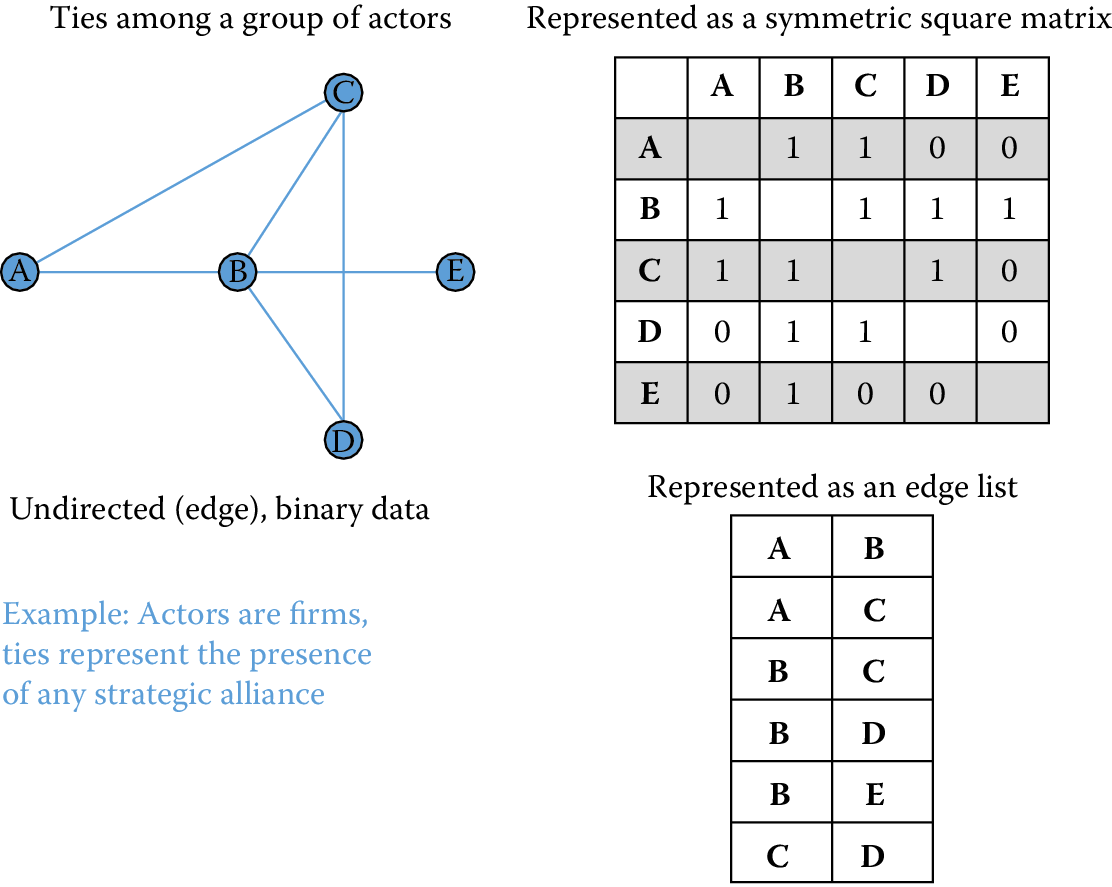
\includegraphics[width=0.7\linewidth]{ChapterNetworks/figures/fig8-1} 

}

\caption{Undirected, binary, one-mode network data}\label{fig:fig8-1}
\end{figure}

A much more complicated network would be one that is both directed and
valued. One example might be a network of nations connected by flows of
international trade. Goods and services flow from one nation to another
and the value of those goods and services (or their volume) represents
ties of different strengths. When networks connecting one class of nodes
(in this case nations) are directed and valued, they can be represented
as asymmetric valued matrices or lists of arcs with associated values.
(See Figure \ref{fig:fig8-1}.)

\begin{figure}

{\centering \includegraphics[width=0.7\linewidth]{ChapterNetworks/figures/fig8-2} 

}

\caption{Directed, valued, one-mode network data}\label{fig:fig8-2}
\end{figure}

Many studies of small- to medium-sized social networks rely on one-mode
data. Large-scale social network data of this type are relatively rare,
but one-mode data of this sort are fairly common in relationships among
other types of nodes such as web pages or citations connecting patents
or publications. Nevertheless, much ``big'' social network analysis is
conducted using two-mode data. The UMETRICS employee data set is a
two-mode network that connects people (research employees) to the grants
that pay their wages. These two types of nodes can be represented as a
rectangular matrix that is either valued or binary. It is relatively
rare to analyze untransformed two-mode network data. Instead, most
analyses take advantage of the fact that such networks are \emph{dual}
(White, Boorman, and Breiger
\protect\hyperlink{ref-white1976social}{1976}). In other words, a
two-mode network connecting grants and people can be conceptualized (and
analyzed) as two one-mode networks, or \emph{projections}\footnote{Key
  insight: A two-mode network can be conceptualized and analyzed as two
  one-mode networks, or projections.}.

\subsection{Inducing one-mode networks from two-mode
data}\label{inducing-one-mode-networks-from-two-mode-data}

The most important trick in large-scale social network analysis is that
of inducing one-mode, or unipartite, networks (e.g., employee \(\times\)
employee relationships) from two-mode, or bipartite, data. But the
ubiquity and potential value of two-mode data can come at a cost. Not
all affiliations are equally likely to represent real, meaningful
relationships. While it seems plausible to assume that two individuals
paid by the same grant have interactions that reasonably pertain to the
work funded by the grant, this need not be the case.

For example, consider the two-mode grant \(\times\) person network for
university A. I used SQL to create a representation of this network that
is readable by a freeware network visualization program called Pajek
(Batagelj and Mrvar \protect\hyperlink{ref-batagelj1998pajek}{1998}). In
this format, a network is represented as two lists: a \emph{vertex list}
that lists the nodes in the graph and an \emph{edge list} that lists the
connections between those nodes. In our grant \(\times\) person network,
we have two types of nodes, people and grants, and one kind of edge,
used to represent wage payments from grants to individuals.

I present a brief snippet of the resulting network file in what follows,
showing first the initial 10 elements of the vertex list and then the
initial 10 elements of the edge list, presented in two columns for
compactness. (The complete file comprises information on 9,206 employees
and 3,389 grants, for a total of 12,595 vertices and 15,255 edges. The
employees come first in the vertex list, and so the 10 rows shown below
all represent employees.) Each vertex is represented by a vertex
number--label pair and each edge by a pair of vertices plus an optional
value. Thus, the first entry in the edge list (1 10419) specifies that
the vertex with identifier 1 (which happens to be the first element of
the vertex list, which has value ``00100679'') is connected to the
vertex with identifier 10419 by an edge with value 1, indicating that
employee ``00100679'' is paid by the grant described by vertex 10419.

*Grant-Person-Network

\begin{longtable}[]{@{}llll@{}}
\toprule
*Vertices 12595 9206 & & *Edges &\tabularnewline
\midrule
\endhead
1 & ``00100679'' & 1 & 10419\tabularnewline
2 & ``00107462'' & 2 & 10422\tabularnewline
3 & ``00109569'' & 3 & 9855\tabularnewline
4 & ``00145355'' & 3 & 9873\tabularnewline
5 & ``00153190'' & 4 & 9891\tabularnewline
6 & ``00163131'' & 7 & 10432\tabularnewline
7 & ``00170348'' & 7 & 12226\tabularnewline
8 & ``00172339'' & 8 & 10419\tabularnewline
9 & ``00176582'' & 9 & 11574\tabularnewline
10 & ``00203529'' & 10 & 11196\tabularnewline
\bottomrule
\end{longtable}

The network excerpted above is two-mode because it represents
relationships between two different classes of nodes, grants, and
people. In order to use data of this form to address questions about
patterns of collaboration on UMETRICS campuses, we must first transform
it to represent collaborative relationships.

A person-by-person projection of the original two-mode network assumes
that ties exist between people when they are paid by the same grant. By
the same token, a grant-by-grant projection of the original two-mode
network assumes that ties exist between grants when they pay the same
people. Transforming two-mode data into one-mode projections is a fairly
simple matter. If \(\mathbf{X}\) is a rectangular matrix,
\(p \times g\), then a one-mode projection, \(p \times p\), can be
obtained by multiplying \(\mathbf{X}\) by its transpose \(\mathbf{X}'\).
Figure \ref{fig:fig8-3} summarizes this transformation.

\begin{figure}

{\centering \includegraphics[width=0.7\linewidth]{ChapterNetworks/figures/fig8-3} 

}

\caption{Two-mode affiliation data}\label{fig:fig8-3}
\end{figure}

In the following snippet of code, I use the \texttt{igraph} package in
Python to read in a Pajek file and then transform the original two-mode
network into two separate projections. Because my focus in this
discussion is on relationships among people, I then move on to work
exclusively with the employee-by-employee projection. However, every
technique that I describe below can also be used with the grant-by-grant
projection, which provides a different view of how federally funded
research is put together by collaborative relationships on campus.

\begin{Shaded}
\begin{Highlighting}[]
\ImportTok{from}\NormalTok{ igraph }\ImportTok{import} \OperatorTok{*}

\CommentTok{# Read the graph}
\NormalTok{g }\OperatorTok{=}\NormalTok{ Graph.Read_Pajek(}\StringTok{"public_a_2m.net"}\NormalTok{)}

\CommentTok{# Look at result}
\NormalTok{summary(g)}


\CommentTok{# IGRAPH U-WT 12595 15252 --}
\CommentTok{# + attr: color (v), id (v), shape (v), type (v), x (v), y (v), z (v), weight (e)}
\CommentTok{# ...}
\CommentTok{# ...}

\CommentTok{# Transform to get 1M projection}
\NormalTok{pr_g_proj1, pr_g_proj2}\OperatorTok{=}\NormalTok{ g.bipartite_projection()}

\CommentTok{# Look at results}
\NormalTok{summary(pr_g_proj1)}

\CommentTok{# IGRAPH U-WT 9206 65040 --}
\CommentTok{# + attr: color (v), id (v), shape (v), type (v), x (v), y (v), z (v), weight (e)}

\NormalTok{summary(pr_g_proj2)}
\CommentTok{# IGRAPH U-WT 3389 12510 --}
\CommentTok{# + attr: color (v), id (v), shape (v), type (v), x (v), y (v), z (v), weight (e)}

\CommentTok{# pr_g_proj1 is the employeeXemployee projection, n=9,206 nodes}
\CommentTok{# Rename to emp for use in future calculations}

\NormalTok{emp}\OperatorTok{=}\NormalTok{pr_g_proj1}
\end{Highlighting}
\end{Shaded}

We now can work with the graph \texttt{emp}, which represents the
collaborative network of federally funded research on this campus. Care
must be taken when inducing one-mode network projections from two-mode
network data because not all affiliations provide equally compelling
evidence of actual social relationships. While assuming that people who
are paid by the same research grants are collaborating on the same
project seems plausible, it might be less realistic to assume that all
students who take the same university classes have meaningful
relationships. For the remainder of this chapter, the examples I discuss
are based on UMETRICS employee data rendered as a one-mode
person-by-person projection of the original two-mode person-by-grants
data. In constructing these networks I assume that a tie exists between
two university research employees when they are paid any wages from the
same grant during the same year. Other time frames or thresholds might
be used to define ties if appropriate for particular analyses\footnote{Key
  insight: Care must be taken when inducing one-mode network projections
  from two-mode network data because not all affiliations provide
  equally compelling evidence of actual social relationships.}.

\section{Network measures}\label{network-measures}

The power of networks lies in their unique flexibility and ability to
address many phenomena at multiple levels of analysis. But harnessing
that power requires calculating measures that take into account the
overall structure of relationships represented in a given network. The
key insight of structural analysis is that outcomes for any individual
or group are a function of the complete pattern of connections among
them. In other words, the explanatory power of networks is driven as
much by the pathways that \emph{indirectly} connect nodes as by the
particular relationships that \emph{directly} link members of a given
dyad. Indirect ties create reachability in a network\footnote{Key
  insight: Structural analysis of outcomes for any individual or group
  are a function of the complete pattern of connections among them.}.

\subsection{Reachability}\label{reachability}

Two nodes are said to be reachable when they are connected by an
unbroken chain of relationships through other nodes. For instance, two
people who have never met may nonetheless be able to reach each other
through a common acquaintance who is positioned to broker an
introduction (Obstfeld \protect\hyperlink{ref-obstfeld2005social}{2005})
or the transfer of information and resources (Burt
\protect\hyperlink{ref-burt2004structural}{2004}). It is the
reachability that networks create that makes them so important for
understanding the work of science and innovation.

Consider Figure \ref{fig:fig8-4}, which presents three schematic
networks. In each, one focal node, ego, is colored orange. Each ego has
four alters, but the fact that each has connections to four other nodes
masks important differences in their structural positions. Those
differences have to do with the number of other nodes they can reach
through the network and the extent to which the other nodes in the
network are connected to each other. The orange node (ego) in each
network has four partners, but their positions are far from equivalent.
Centrality measures on full network data can tease out the differences.
The networks also vary in their gross characteristics. Those
differences, too, are measurable\footnote{Key insight: Much of the power
  of networks (and their systemic features) is due to indirect ties that
  create reachability. Two nodes can reach each other if they are
  connected by an unbroken chain of relationships. These are often
  called indirect ties.}.

\begin{figure}

{\centering \includegraphics[width=0.7\linewidth]{ChapterNetworks/figures/fig8-4} 

}

\caption{Reachability and indirect ties}\label{fig:fig8-4}
\end{figure}

Networks in which more of the possible connections among nodes are
realized are denser and more cohesive than networks in which fewer
potential connections are realized. Consider the two smaller networks in
Figure \ref{fig:fig8-4}, each of which is comprised of five nodes. Just
five ties connect those nodes in the network on the far right of the
figure. One smaller subset of that network, the triangle connecting ego
and two alters at the center of the image, represents a more cohesively
connected subset of the networks. In contrast, eight of the nine ties
that are possible connect the five nodes in the middle figure; no subset
of those nodes is clearly more interconnected than any other. While
these kinds of differences may seem trivial, they have implications for
the orange nodes, and for the functioning of the networks as a whole.
Structural differences between the positions of nodes, the presence and
characteristics of cohesive ``communities'' within larger networks
(Girvan and Newman \protect\hyperlink{ref-girvan2002community}{2002}),
and many important properties of entire structures can be quantified
using different classes of network measures. Newman
(\protect\hyperlink{ref-newman2010networks}{2010}) provides the most
recent and most comprehensive look at measures and algorithms for
network research.

The most essential thing to be able to understand about larger scale
networks is the pattern of indirect connections among nodes. What is
most important about the structure of networks is not necessarily the
ties that link particular pairs of nodes to one another. Instead, it is
the chains of indirect connections that make networks function as a
system and thus make them worthwhile as new levels of analysis for
understanding social and other dynamics.

\subsection{Whole-network measures}\label{whole-network-measures}

The basic terms needed to characterize whole networks are fairly simple.
It is useful to know the size (in terms of nodes and ties) of each
network you study. This is true both for the purposes of being able to
generally gauge the size and connectivity of an entire network and
because many of the measures that one might calculate using such
networks should be standardized for analytic use. While the list of
possible network measures is long, a few commonly used indices offer
useful insights into the structure and implications of entire network
structures.

\textbf{Components and reachability}

As we have seen, a key feature of networks is reachability. The
reachability of participants in a network is determined by their
membership in what network theorists call \emph{components}, subsets of
larger networks where every member of a group is indirectly connected to
every other. If you imagine a standard node and line drawing of a
network, a component is a portion of the network where you can trace
paths between every pair of nodes without ever having to lift your pen.

Most large networks have a single dominant component that typically
includes anywhere from 50\% to 90\% of its participants as well as many
smaller components and isolated nodes that are disconnected from the
larger portion of the network. Because the path length centrality
measures described below can only be computed on connected subsets of
networks, it is typical to analyze the largest component of any given
network. Thus any description of a network or any effort to compare
networks should report the number of components and the percentage of
nodes reachable through the largest component. In the code snippet
below, I identify the weakly connected components of the employee
network, \texttt{emp}.

\begin{Shaded}
\begin{Highlighting}[]
\CommentTok{# Add component membership}
\NormalTok{emp.vs[}\StringTok{"membership"}\NormalTok{] }\OperatorTok{=}\NormalTok{ emp.clusters(mode}\OperatorTok{=}\StringTok{"weak"}\NormalTok{).membership}

\CommentTok{# Add component size}
\NormalTok{emp.vs[}\StringTok{"csize"}\NormalTok{] }\OperatorTok{=}\NormalTok{ [emp.clusters(mode}\OperatorTok{=}\StringTok{"weak"}\NormalTok{).sizes()[i] }\ControlFlowTok{for}\NormalTok{ i }\KeywordTok{in}\NormalTok{ emp.clusters(mode}\OperatorTok{=}\StringTok{"weak"}\NormalTok{).membership]}

\CommentTok{# Identify the main component}
\CommentTok{# Get indices of max clusters}
\NormalTok{maxSize }\OperatorTok{=} \BuiltInTok{max}\NormalTok{(emp.clusters(mode}\OperatorTok{=}\StringTok{"weak"}\NormalTok{).sizes())}
\NormalTok{emp.vs[}\StringTok{"largestcomp"}\NormalTok{] }\OperatorTok{=}\NormalTok{ [}\DecValTok{1} \ControlFlowTok{if}\NormalTok{ maxSize }\OperatorTok{==}\NormalTok{ x }\ControlFlowTok{else} \DecValTok{0} \ControlFlowTok{for}\NormalTok{ x }\KeywordTok{in}\NormalTok{ emp.vs[}\StringTok{"csize"}\NormalTok{]]}

\CommentTok{# Add component membership}

\NormalTok{emp.vs[}\StringTok{"membership"}\NormalTok{] }\OperatorTok{=}\NormalTok{ emp.clusters(mode}\OperatorTok{=}\StringTok{"weak"}\NormalTok{).membership}
\end{Highlighting}
\end{Shaded}

The main component of a network is commonly analyzed and visualized
because the graph-theoretic distance among unconnected nodes is
infinite, which renders calculation of many common network measures
impossible without strong assumptions about just how far apart
unconnected nodes actually are. While some researchers replace infinite
path lengths with a value that is one plus the longest path, called the
network's diameter, observed in a given structure, it is also common to
simply analyze the largest connected component of the network.

\textbf{Path length}

One of the most robust and reliable descriptive statistics about an
entire network is the average path length, \(l_{G}\), among nodes.
Networks with shorter average path lengths have structures that may make
it easier for information or resources to flow among members in the
network. Longer path lengths, by comparison, are associated with greater
difficulty in the diffusion and transmission of information or
resources. Let \(g\) be the number of nodes or vertices in a network.
Then \[l_G=\frac{1}{g(g-1)}\sum_{i\neq j}d(n_i,n_j),\] where
\(d(n_i,n_j)\) is the path length between \(n_i\) and \(n_j\).
Typically, the path length is defined as the length of the shortest
path\footnote{A \emph{shortest path} is a path that requires the fewest
  steps, taking into account values of ties if applicable. In networks
  with unvalued ties, most pairs have several of those. In networks with
  valued ties, the shortest path may not be the one with the fewest
  vertices.} between two nodes.

As with other measures based on reachability, it is most common to
report the average path length for the largest connected component of
the network because the graph-theoretic distance between two unconnected
nodes is infinite. In an electronic network such as the World Wide Web,
a shorter path length means that any two pages can be reached through
fewer hyperlink clicks.

The snippet of code below identifies the distribution of shortest path
lengths among all pairs of nodes in a network and the average path
length. I also include a line of code that calculates the network
distance among all nodes and returns a matrix of those distances. That
matrix (saved as \texttt{empdist}) can be used to calculate additional
measures or to visualize the graph-theoretic proximities among nodes.

\begin{Shaded}
\begin{Highlighting}[]
\CommentTok{# Calculate distances and construct distance table}

\NormalTok{dfreq}\OperatorTok{=}\NormalTok{emp.path_length_hist(directed}\OperatorTok{=}\VariableTok{False}\NormalTok{)}
\BuiltInTok{print}\NormalTok{(dfreq)}

\CommentTok{# N = 12506433, mean +- sd: 5.0302 +- 1.7830}
\CommentTok{# Each * represents 51657 items}
\CommentTok{# [ 1,  2): * (65040)}
\CommentTok{# [ 2,  3): ********* (487402)}
\CommentTok{# [ 3,  4): *********************************** (1831349)}
\CommentTok{# [ 4,  5): ********************************************************** (2996157)}
\CommentTok{# [ 5,  6): **************************************************** (2733204)}
\CommentTok{# [ 6,  7): ************************************** (1984295)}
\CommentTok{# [ 7,  8): ************************ (1267465)}
\CommentTok{# [ 8,  9): ************ (649638)}
\CommentTok{# [ 9, 10): ***** (286475)}
\CommentTok{# [10, 11): ** (125695)}
\CommentTok{# [11, 12): * (52702)}
\CommentTok{# [12, 13):  (18821)}
\CommentTok{# [13, 14):  (5944)}
\CommentTok{# [14, 15):  (1682)}
\CommentTok{# [15, 16):  (403)}
\CommentTok{# [16, 17):  (128)}
\CommentTok{# [17, 18):  (28)}
\CommentTok{# [18, 19):  (5)}
\BuiltInTok{print}\NormalTok{(dfreq.unconnected)}
\CommentTok{# 29864182}

\BuiltInTok{print}\NormalTok{(emp.average_path_length(directed}\OperatorTok{=}\VariableTok{False}\NormalTok{))}
\CommentTok{#[1] 5.030207}

\NormalTok{empdist}\OperatorTok{=}\NormalTok{ emp.shortest_paths()}
\end{Highlighting}
\end{Shaded}

These measures provide a few key insights into the employee network we
have been considering. First, the average pair of nodes that are
connected by indirect paths are slightly more than five steps from one
another. Second, however, many node pairs in this network
(\texttt{\$unconnected} = 29,864,182) are unconnected and thus
unreachable to each other. Figure \ref{fig:fig8-5} presents a histogram
of the distribution of path lengths in the network. It represents the
numeric values returned by the \texttt{distance.table} command in the
code snippet above. In this case the diameter of the network is 18 and
five pairs of nodes are reachable at this distance, but the largest
group of dyads is reachable (\(N=2{,}996{,}157\) dyads) at distance 4.
In short, nearly 3 million pairs of nodes are collaborators of
collaborators of collaborators of collaborators.

\begin{figure}

{\centering \includegraphics[width=0.7\linewidth]{ChapterNetworks/figures/fig8-5} 

}

\caption{Histogram of path lengths for university A employee network}\label{fig:fig8-5}
\end{figure}

\textbf{Degree distribution}

Another powerful way to describe and compare networks is to look at the
distribution of centralities across nodes. While any of the centrality
measures described above could be summarized in terms of their
distribution, it is most common to plot the degree distribution of large
networks. Degree distributions commonly have extremely long tails. The
implication of this pattern is that most nodes have a small number of
ties (typically one or two) and that a small percentage of nodes account
for the lion's share of a network's connectivity and reachability.
Degree distributions are typically so skewed that it is common practice
to plot degree against the percentage of nodes with that degree score on
a log--log scale.

High-degree nodes are often particularly important actors. In the
UMETRICS networks that are employee \(\times\) employee projections of
employee \(\times\) grant networks, for instance, the nodes with the
highest degree seem likely to include high-profile faculty---the
investigators on larger institutional grants such as National Institutes
of Health-funded Clinical and Translational Science Awards and National
Science Foundation-funded Science and Technology Centers, and perhaps
staff whose particular skills are in demand (and paid for) by multiple
research teams. For instance, the head technician in a core microscopy
facility or a laboratory manager who serves multiple groups might appear
highly central in the degree distribution of a UMETRICS network.

Most importantly, the degree distribution is commonly taken to provide
insight into the dynamics by which a network was created. Highly skewed
degree distributions often represent scale-free networks (Powell et al.
\protect\hyperlink{ref-powell2005network}{2005}; Barabási and Albert
\protect\hyperlink{ref-barabasi1999emergence}{1999}; Newman
\protect\hyperlink{ref-newman2005measure}{2005}), which grow in part
through a process called \emph{preferential attachment}, where new nodes
entering the network are more likely to attach to already prominent
participants. In the kinds of scientific collaboration networks that
UMETRICS represents, a scale-free degree distribution might come about
as faculty new to an institution attempt to enroll more established
colleagues on grants as coinvestigators. In the comparison exercise
outlined below, I plot degree distributions for the main components of
two different university networks.

\textbf{Clustering coefficient}

The third commonly used whole-network measure captures the extent to
which a network is cohesive, with many nodes interconnected. In networks
that are more cohesively clustered, there are fewer opportunities for
individuals to play the kinds of brokering roles that we will discuss
below in the context of betweenness centrality. Less cohesive networks,
with lower levels of clustering, are potentially more conducive to
brokerage and the kinds of innovation that accompany it.

However, the challenge of innovation and discovery is both the moment of
invention, the ``aha!'' of a good new idea, and the often complicated,
uncertain, and collaborative work that is required to turn an initial
insight into a scientific finding. While less clustered, open networks
are more likely to create opportunities for brokers to develop fresh
ideas, more cohesive and clustered networks support the kinds of
repeated interactions, trust, and integration that are necessary to do
uncertain and difficult collaborative work.

While it is possible to generate a global measure of cohesiveness in
networks, which is generically the number of closed triangles (groups of
three nodes all connected to one another) as a proportion of the number
of possible triads, it is more common to take a local measure of
connectivity and average it across all nodes in a network. This local
connectivity measure more closely approximates the notion of cohesion
around nodes that is at the heart of studies of networks as means to
coordinate difficult, risky work. The code snippet below calculates both
the global clustering coefficient and a vector of node-specific
clustering coefficients whose average represents the local measure for
the employee \(\times\) employee network projection of the university A
UMETRICS data.

\begin{Shaded}
\begin{Highlighting}[]
\CommentTok{# Calculate clustering coefficients}
\NormalTok{emp.transitivity_undirected()}
\CommentTok{# 0.7241}

\NormalTok{local_clust}\OperatorTok{=}\NormalTok{emp.transitivity_local_undirected(mode}\OperatorTok{=}\StringTok{"zero"}\NormalTok{)}
\CommentTok{# (isolates="zero" sets clustering to zero rather than undefined)}

\ImportTok{import}\NormalTok{ pandas }\ImportTok{as}\NormalTok{ pd}
\BuiltInTok{print}\NormalTok{(pd.Series(local_clust).describe())}
\CommentTok{# count    9206.000000}
\CommentTok{# mean        0.625161}
\CommentTok{# std         0.429687}
\CommentTok{# min         0.000000}
\CommentTok{# 25%         0.000000}
\CommentTok{# 50%         0.857143}
\CommentTok{# 75%         1.000000}
\CommentTok{# max         1.000000}
\CommentTok{#--------------------------------------------------#}
\end{Highlighting}
\end{Shaded}

Together, these summary statistics---number of nodes, average path
length, distribution of path lengths, degree distribution, and the
clustering coefficient---offer a robust set of measures to examine and
compare whole networks. It is also possible to distinguish among the
positions nodes hold in a particular network. Some of the most powerful
centrality measures also rely on the idea of indirect ties\footnote{Key
  insight: Some of the most powerful centrality measures also rely on
  the idea of indirect ties.}.

\textbf{Centrality measures}

This class of measures is the most common way to distinguish between the
positions individual nodes hold in networks. There are many different
measures of centrality that capture different aspects of network
positions, but they fall into three general types. The most basic and
intuitive measure of centrality, \emph{degree centrality,} simply counts
the number of ties that a node has. In a binary undirected network, this
measure resolves into the number of unique alters each node is connected
to. In mathematical terms it is the row or column sum of the adjacency
matrix that characterizes a network. Degree centrality,
\(C_{D}(n_{i})\), represents a clear measure of the prominence or
visibility of a node. Let \[C_D(n_i)=\sum_jx_{ij}.\] The degree of a
node is limited by the size of the network in which it is embedded. In a
network of \(g\) nodes the maximum degree of any node is \(g-1\). The
two orange nodes in the small networks presented in Figure
\ref{fig:fig8-4} have the maximum degree possible (4). In contrast, the
orange node in the larger, 13-node network in that figure has the same
number of alters but the possible number of partners is three times as
large (12). For this reason it is problematic to compare raw degree
centrality measures across networks of different sizes. Thus, it is
common to normalize degree by the maximum value defined by \(g-1\):
\[C_D^{\prime}(n_i)=\frac{\sum_j x_{ij}}{g-1}.\]

While the normalized degree centrality of the two orange nodes of the
smaller networks in Figure \ref{fig:fig8-4} is 1.0, the normalized value
for the node in the large network of 13 nodes is 0.33. Despite the fact
that the highlighted nodes in the two smaller networks have the same
degree centrality, the pattern of indirect ties connecting their alters
means they occupy meaningfully different positions. There are a number
of degree-based centrality measures that take more of the structural
information from a complete network into account by using a variety of
methods to account not just for the number of partners a particular ego
might have but also for the prominence of those partners. Two well-known
examples are eigenvector centrality and page rank (see Newman
(\protect\hyperlink{ref-newman2010networks}{2010}) Ch. 7.2 and 8.4).

Consider two additional measures that capture aspects of centrality that
have more to do with the indirect ties that increase reachability. Both
make explicit use of the idea that reachability is the source of many of
the important social and economic benefits of salutary network
positions, but they do so with different substantive emphases. Both of
these approaches rely on the idea of a network geodesic, the shortest
path connecting any pair of actors. Because these measures rely on
reachability, they are only useful when applied to components. When
nodes have no ties (degree 0) they are called \emph{isolates}. The
geodesic distances are infinite and thus path-based centrality measures
cannot be calculated. This is a shortcoming of these measures, which can
only be used on connected subsets of graphs where each node has at least
one tie to another and all are indirectly connected.

Closeness centrality, \(C_{C,}\) is based on the idea that networks
position some individuals closer to or farther away from other
participants. The primary idea is that shorter network paths between
actors increase the likelihood of communication and with it the ability
to coordinate complicated activities. Let \(d(n_{i}, n_{j})\) represent
the number of network steps in the geodesic path connecting two nodes
\(i\) and \(j\). As \(d\) increases, the network distance between a pair
of nodes grows. Thus a standard measure of closeness is the inverse of
the sum of distances between any given node and all the others that are
reachable in a network: \[C_C(n_i) = \frac{1}{\sum_{j=1}^gd(n_i,n_j)}.\]
The maximum of closeness centrality occurs when a node is directly
connected to every possible partner in the network. As with degree
centrality, closeness depends on the number of nodes in a network. Thus,
it is necessary to standardize the measure to allow comparisons across
multiple networks:
\[C_C^{\prime}(n_i)=\frac{g-1}{\sum_{j=1}^gd(n_i,n_j)}.\]

Like closeness centrality, betweenness centrality, \(C_{B}\), relies on
the concept of geodesic paths to capture nuanced differences the
positions of nodes in a connected network. Where closeness assumes that
communication and the flow of information increase with proximity,
betweenness captures the idea of brokerage that was made famous by Burt
(\protect\hyperlink{ref-burt1993social}{1993}). Here too the idea is
that flows of information and resources pass between nodes that are not
directly connected through indirect paths. The key to the idea of
brokerage is that such paths pass through nodes that can interdict, or
otherwise profit from their position ``in between'' unconnected alters.
This idea has been particularly important in network studies of
innovation (Owen-Smith and Powell
\protect\hyperlink{ref-owen2003expanding}{2003}; Burt
\protect\hyperlink{ref-burt2004structural}{2004}), where flows of
information through strategic alliances among firms or social networks
connecting individuals loom large in explanations of why some
organizations or individuals are better able to develop creative ideas
than others.

To calculate betweenness as originally specified, two strong assumptions
are required (Freeman
\protect\hyperlink{ref-freeman1979centrality}{1979}). First, one must
assume that when people (or organizations) search for new information
through their networks, they are capable of identifying the shortest
path to what they seek. When multiple paths of equal length exist, we
assume that each path is equally likely to be used. Newman
(\protect\hyperlink{ref-newman2005measure}{2005}) describes an
alternative betweenness measure based on random paths through a network,
rather than shortest paths, that relaxes these assumptions. For now, let
\(g_{jk}\) equal the number of geodesic paths linking any two actors.
Then \(1/g_{jk}\) is the probability that any given path will be
followed on a particular node's search for information or resources in a
network. In order to calculate the betweenness score of a particular
actor, \(i\), it is then necessary to determine how many of the geodesic
paths connecting \(j\) to \(k\) include \(i\). That quantity is
\(g_{jk}(n_{i})\). With these (unrealistic) assumptions in place, we
calculate \(C_{B}(n_{i})\) as
\[C_B(n_i)=\sum_{j<k} g_{jk}^{(n_i)}/g_{jk}.\] Here, too, the maximum
value depends on the size of the network. \(C_{B}(n_{i}) = 1\) if \(i\)
sits on every geodesic path in the network. While this is only likely to
occur in small, star-shaped networks, it is still common to standardize
the measure. Instead of conceptualizing network size in terms of the
number of nodes, however, this measure requires that we consider the
number of possible pairs of actors (excluding ego) in a structure. When
there are \(g\) nodes, that quantity is \((g-1)(g-2)/2\) and the
standardized betweenness measure is
\[C_B^{\prime}(n_i)=\frac{C_B(n_i)}{(g-1)(g-2)/2}.\]

Centrality measures of various sorts are the most commonly used means to
examine network effects at the level of individual participants in a
network. In the context of UMETRICS, such indices might be applied to
examine the differential scientific or career success of graduate
students as a function of their positions in the larger networks of
their universities. In such an analysis, care must be taken to use the
standardized measures as university collaboration networks can vary
dramatically in size and structure. Describing and accounting for such
variations and the possibility of analyses conducted at the level of
entire networks or subsets of networks, such as teams and labs, requires
a different set of measures. The code snippet presented below calculates
each of these measures for the university A employee network we have
been examining.

\begin{Shaded}
\begin{Highlighting}[]
\CommentTok{# Calculate centrality measures}
\NormalTok{emp.vs[}\StringTok{"degree"}\NormalTok{]}\OperatorTok{=}\NormalTok{emp.degree()}
\NormalTok{emp.vs[}\StringTok{"close"}\NormalTok{]}\OperatorTok{=}\NormalTok{emp.closeness(vertices}\OperatorTok{=}\NormalTok{emp.vs)}
\NormalTok{emp.vs[}\StringTok{"btc"}\NormalTok{]}\OperatorTok{=}\NormalTok{emp.betweenness(vertices}\OperatorTok{=}\NormalTok{emp.vs, directed}\OperatorTok{=}\VariableTok{False}\NormalTok{)}
\end{Highlighting}
\end{Shaded}

\section{Case Study: Comparing collaboration
networks}\label{case-study-comparing-collaboration-networks}

Consider Figure \ref{fig:fig8-6}, which presents visualizations of the
main component of two university networks. Both of these representations
are drawn from a single year (2012) of UMETRICS data. Nodes represent
people, and ties reflect the fact that those individuals were paid with
the same federal grant in the same year. The images are scaled so that
the physical location of any node is a function of its position in the
overall pattern of relationships in the network. The size and color of
nodes represent their betweenness centrality. Larger, darker nodes are
better positioned to play the role of brokers in the network. A complete
review of the many approaches to network visualization and their dangers
in the absence of descriptive statistics such as those presented above
is beyond the scope of this chapter, but consider the guidelines
presented in Chapter \protect\hyperlink{chap:viz}{Information
Visualization} on information visualization as well as useful
discussions by Powell et al.
(\protect\hyperlink{ref-powell2005network}{2005}) and Healy and Moody
(\protect\hyperlink{ref-healy2014data}{2014}).

Consider the two images. University A is a major public institution with
a significant medical school. University B, likewise, is a public
institution but lacks a medical school. It is primarily known for strong
engineering. The two networks manifest some interesting and suggestive
differences. Note first that the network on the left (university A)
appears much more tightly connected. There is a dense center and there
are fewer very large nodes whose positions bridge less well-connected
clusters. Likewise, the network on the right (university B) seems at a
glance to be characterized by a number of densely interconnected groups
that are pulled together by ties through high-degree brokers. One part
of this may have to do with the size and structure of university A's
medical school, whose significant NIH funding dominates the network. In
contrast, university B's engineering-dominated research portfolio seems
to be arranged around clusters of researchers working on similar topic
areas and lacks the dominant central core apparent in university B's
image.

The implications of these kinds of university-level differences are just
starting to be realized, and the UMETRICS data offer great possibilities
for exactly this kind of study. These networks, in essence, represent
the local social capacity to respond to new problems and to develop
scientific findings. Two otherwise similar institutions might have quite
different capabilities based on the structure and composition of their
collaboration networks.

\begin{figure}

{\centering \includegraphics[width=0.7\linewidth]{ChapterNetworks/figures/fig8-6} 

}

\caption{The main component of two university networks}\label{fig:fig8-6}
\end{figure}

The intuitions suggested by Figure \ref{fig:fig8-6} can also be checked
against some of the measures we have described. Figure
\ref{fig:fig8-7a}, for instance, presents degree distributions for each
of the two networks. Figure \ref{fig:fig8-8} presents the histogram of
path lengths for each network.

\begin{center}\includegraphics[width=0.7\linewidth]{ChapterNetworks/figures/fig8-7a} \end{center}\begin{figure}

{\centering \includegraphics[width=0.7\linewidth]{ChapterNetworks/figures/fig8-7b} 

}

\caption{Degree distribution for two universities}\label{fig:fig8-7a}
\end{figure}

It is evident from Figure \ref{fig:fig8-7a} that they are quite
different in character. University A's network follows a more classic
skewed distribution of the sort that is often associated with the kinds
of power-law degree distributions common to scale-free networks. In
contrast, university B's distribution has some interesting features.
First, the left-hand side of the distribution is more dispersed than it
is for university A, suggesting that there are many nodes with moderate
degree. These nodes may also have high betweenness centrality if their
ties allow them to span different subgroups within the networks. Of
course this might also reflect the fact that each cluster also has
members that are more locally prominent. Finally, consider the few
instances on the right-hand end of the distribution where there are
relatively large numbers of people with surprisingly high degree. I
suspect these are the result of large training grants or center grants
that employ many people. A quirk of relying on one-mode projections of
two-mode data is that every person associated with a particular grant is
connected to every other. More work needs to be done to bear out these
hypotheses, but for now it suffices to say that the degree distribution
of the networks bears out the intuition we drew from the images that
they are significantly different.

\begin{figure}

{\centering \includegraphics[width=0.7\linewidth]{ChapterNetworks/figures/fig8-8} 

}

\caption{Distribution of path lengths for universities A and B}\label{fig:fig8-8}
\end{figure}

The path length histogram presented in Figure \ref{fig:fig8-8} suggests
a similar pattern. While the average distance among any pair of
connected nodes in both networks is fairly similar (see Table
\ref{tab:table8-1}, university B has a larger number of unconnected
nodes and university A has a greater concentration of more closely
connected dyads. The preponderance of shorter paths in this network
could also be a result of a few larger grants that connect many pairs of
nodes at unit distance and thus shorten overall path lengths.

\begin{longtable}[]{@{}lcc@{}}
\caption{\label{tab:table8-1} Descriptive statistics for the main components
of two university networks}\tabularnewline
\toprule
& \textbf{University A} & \textbf{University B}\tabularnewline
\midrule
\endfirsthead
\toprule
& \textbf{University A} & \textbf{University B}\tabularnewline
\midrule
\endhead
Nodes & 4,999 & 4,144\tabularnewline
Edges (total) & 57,756 & 91,970\tabularnewline
\% nodes in main component & 68.67\% & 67.34\%\tabularnewline
Diameter & 18 & 18\tabularnewline
Average degree & 11.554 & 44.387\tabularnewline
Clustering coefficient & 0.855 & 0.913\tabularnewline
Density & 0.005 & 0.011\tabularnewline
Average path length & 5.034 & 5.463\tabularnewline
\bottomrule
\end{longtable}

But how do the descriptive statistics shake out? Table
\ref{tab:table8-1} presents the basic descriptive statistics we have
discussed for each network. University A's network includes 855 more
nodes than university B's, a difference of about 20\%. In contrast,
there are far fewer edges connecting university A's research employees
than connecting university B's, a difference that appears particularly
starkly in the much higher density of university B's network. Part of
the story can be found in the average degree of nodes in each network.
As the degree distributions presented in Figure \ref{fig:fig8-6}
suggested, the average researcher at university B is much more highly
connected to others than is the case at university A. The difference is
stark and quite likely has to do with the presence of larger grants that
employ many individuals.

Both schools have a low average path length (around 5), suggesting that
no member of the network is more than five acquaintances away from any
other. Likewise, the diameter of both networks is 18, which means that
on each campus the most distant pair of nodes is separated by just 18
steps. University A's slightly lower path length may be accounted for by
the centralizing effect of its large medical school grant
infrastructure. Finally, consider the clustering coefficient. This
measure approaches 1 as it becomes more likely that two partners to a
third node will themselves be connected. The likelihood that
collaborators of collaborators will collaborate is high on both
campuses, but substantially higher at university B.

\section{Summary}\label{summary-6}

This chapter has provided a brief overview of the basics of networks and
how to do large-scale network analysis. While network measures can
produce new and exciting ways to characterize social dynamics, they are
also important levels of analysis in their own right. Concepts such as
reachability, cohesion, brokerage, and reciprocity are important, for a
variety of reasons---they can be used to describe networks in terms of
their composition and community structure. This chapter provides a
classic example of how well social science meets data science. Social
science is needed to identify the nodes (what is being connected) and
the ties (the relationships that matter) in order to construct the
relevant networks. Computer science is necessary to collect and
structure the data in a fashion that is sufficient for analysis. The
combination of data science and social science is key to making the
right measurement and visualization decisions.

\section{Resources}\label{resources-4}

For more information about network analysis \emph{in general}, the
International Network for Social Network Analysis
(\url{http://www.insna.org/}) is a large, interdisciplinary association
dedicated to network analysis. It publishes a traditional academic
journal, \emph{Social Networks}, an online journal, \emph{Journal of
Social Structure}, and a short-format journal, \emph{Connections}, all
dedicated to social network analysis. Its several listservs offer
vibrant international forums for discussion of network issues and
questions. Finally, its annual meetings include numerous opportunities
for intensive workshops and training for both beginning and advanced
analysts.

A new journal, \emph{Network Science}
(\url{http://journals.cambridge.org/action/displayJournal?jid=NWS}),
published by Cambridge University Press and edited by a team of
interdisciplinary network scholars, is a good venue to follow for
cutting-edge articles on computational network methods and for
substantive findings from a wide range of social, natural, and
information science applications.

There are some good software packages available. \emph{Pajek}
(\url{http://mrvar.fdv.uni-lj.si/pajek/}) is a freeware package for
network analysis and visualization. It is routinely updated and has a
vibrant user group. Pajek is exceptionally flexible for large networks
and has a number of utilities that allow import of its relatively simple
file types into other programs and packages for network analysis.
\emph{Gephi} (\url{https://gephi.org/}) is another freeware package that
supports large-scale network visualization. Though I find it less
flexible than Pajek, it offers strong support for compelling
visualizations.

\emph{Stanford Network Analysis Platform (SNAP)}
(\textless{}snap.stanford.edu\textgreater{}) is a general purpose
library for network analysis and graph mining. Is scales to very large
networks, efficiently manipulates large graphs, calculates structural
properties, generates regular and random graphs.

\emph{Network Workbench} (\url{http://nwb.cns.iu.edu/}) is a freeware
package that supports extensive analysis and visualization of networks.
This package also includes numerous shared data sets from many different
fields that can used to test and hone your network analytic skills.

\emph{iGraph} (\url{http://igraph.org/redirect.html}) is my preferred
package for network analysis. Implementations are available in R, in
Python, and in C libraries. The examples in this chapter were coded in
iGraph for Python.

\emph{Nexus}
(\url{http://nexus.igraph.org/api/dataset_info?format=html\&limit=10\&offset=20\&operator=or\&order=date})
is a growing repository for network data sets that includes some classic
data dating back to the origins of social science network research as
well as more recent data from some of the best-known publications and
authors in network science.

The \emph{Networks} workbook of Chapter
\protect\hyperlink{chap:workbooks}{Workbooks} provides an introduction
to network analysis and visualizations.\footnote{See
  \url{https://workbooks.coleridgeinitiative.org}.}

\hypertarget{chap:errors}{\chapter{Data Quality and Inference
Errors}\label{chap:errors}}

\textbf{Paul P. Biemer}

This chapter deals with inference and the errors associated with big
data. Social scientists know only too well the cost associated with bad
data---we highlighted both the classic \emph{Literary Digest} example
and the more recent Google Flu Trends problems in Chapter
\protect\hyperlink{chap:intro}{Introduction}. Although the consequences
are well understood, the new types of data are so large and complex that
their properties often cannot be studied in traditional ways. In
addition, the data generating function is such that the data are often
selective, incomplete, and erroneous. Without proper data hygiene, the
errors can quickly compound. This chapter provides, for the first time,
a systematic way to think about the error framework in a big data
setting.

\hypertarget{sec:10-1}{\section{Introduction}\label{sec:10-1}}

The Machine Learning chapter and the Bias and Fairness chapter discuss
how analysis errors can lead to bad inferences and suboptimal decision
making. In fact the whole workflow we depicted in chapter
\protect\hyperlink{chap:intro}{Introduction}---and the decisions made
along the way---can contribute to errors. In this chapter, we will focus
on frameworks that help to detect errors in our data, highlight in
general how errors can lead to incorrect inferences, and discuss some
strategies to mititage the inference risk from errors.

The massive amounts of high-dimensional and unstructured data that have
recently become available to social scientists, such as data from social
media platforms and micro-data from administrative data sources, bring
both new opportunities and new challenges. Many of the problems with
these types of data are well known (see, for example, the AAPOR report
by Japec et al. Japec et al.
(\protect\hyperlink{ref-japec2015big}{2015})): this data often has
selection bias, is incomplete, and erroneous. As it is processed and
analyzed, new errors can be introduced in downstream operations.

These new sources of data are typically aggregated from disparate
sources at various points in time and integrated to form data sets for
further analysis. The processing pipeline involve linking records
together, transforming them to form new attributes (or variables),
documenting the actions taken (although sometimes inadequately), and
interpreting the newly created features of the data. These activities
may introduce new errors into the data set: errors that may be either
\emph{variable} (i.e., errors that create random noise resulting in poor
reliability) or \emph{systematic} (i.e., errors that tend to be
directional, thus exacerbating biases). Using these new sources of data
in statistically valid ways is increasingly challenging in this
environment; however, it is important for social scientists to be aware
of the error risks and the potential effects of these errors on
inferences and decision-making. The massiveness, high dimensionality,
and accelerating pace of data, combined with the risks of variable and
systematic data errors, requires new, robust approaches to data
analysis.

The core issue that is often the cause of these errors is that such data
may not be generated from instruments and methods designed to produce
valid and reliable data for scientific analysis and discovery. Rather,
this is data that are being repurposed for uses not originally intended.
It has been referred to as ``found'' data or ``data exhaust'' because it
is generated for purposes that often do not align with those of the data
analyst. In addition to inadvertent errors, there are also errors from
mischief in the data generation process; for example, automated systems
have been written to generate bogus content in the social media that is
indistinguishable from legitimate or authentic data. Social scientists
using this data must be keenly aware of these limitations and should
take the necessary steps to understand and hopefully mitigate the
effects of hidden errors on their results.

\section{The total error paradigm}\label{sec:10-2}

We now provide a framework for describing, mitigating, and interpreting
the errors in essentially any data set, be it structured or
unstructured, massive or small, static or dynamic. This framework has
been referred to as the total error framework or paradigm. We begin by
reviewing the traditional paradigm, acknowledging its limitations for
truly large and diverse data sets, and we suggest how this framework can
be extended to encompass the new error structures described above.

\subsection{The traditional model}\label{sec:10-2.1}

Dealing with the risks that errors introduce in big data analysis can be
facilitated through a better understanding of the sources and nature of
those errors. Such knowledge is gained through in-depth understanding of
the data generating mechanism, the data processing/transformation
infrastructure, and the approaches used to create a specific data set or
the estimates derived from it. For survey data, this knowledge is
embodied in the well-known \emph{total survey error} (TSE) framework
that identifies all the major sources of error contributing to data
validity and estimator accuracy (Groves
\protect\hyperlink{ref-groves2004survey}{2004}; Biemer and Lyberg
\protect\hyperlink{ref-biemer2003}{2003}; Biemer
\protect\hyperlink{ref-biemer2010total}{2010}). The TSE framework
attempts to describe the nature of the error sources and what they may
suggest about how the errors could affect inference. The framework
parses the total error into bias and variance components that, in turn,
may be further subdivided into subcomponents that map the specific types
of errors to unique components of the total mean squared error. It
should be noted that, while our discussion on issues regarding inference
has quantitative analyses in mind, some of the issues discussed here are
also of interest to more qualitative uses of big data.

For surveys, the TSE framework provides useful insights regarding how
data generating, reformatting, and file preparation processes affect
estimation and inference, and suggest methods for either reducing the
errors at their source or adjusting for their effects in the final
products to produce inferences of higher quality. (Add classic TSE
citations)

The traditional TSE framework is quite general in that it can be applied
to essentially any data set that conform to the format in Figure
\ref{fig:fig10-1}. However, in most practical situations it is quite
limited because it makes no attempt to describe how the processes that
the data may have contributed to what could be construed as data errors.
In some cases, these processes constitute a ``black box,'' and the best
approach is to attempt to evaluate the quality of the end product. For
survey data, the TSE framework provides a fairly complete description of
the error-generating processes for survey data and survey frames (Biemer
\protect\hyperlink{ref-biemer2010total}{2010}). But at this writing,
little effort has been devoted to enumerating the error sources, the
error generating processes for big data. and the effect of these errors
on some common methods for data analysis. Some related articles include
three recent papers that discuss the some of the issues associated with
integrating multiple data sets for official statistics, including the
effects of integration on data uncertainty (see Holmberg and Bycroft
\protect\hyperlink{ref-Holmberg2017}{2017}; Reid, Zabala, and Holmberg
\protect\hyperlink{ref-Reid2017}{2017}; and Zhang
\protect\hyperlink{ref-Zhang2012}{2012}). There has also been some
effort to describe these processes for population registers and
administrative data (Wallgren and Wallgren
\protect\hyperlink{ref-wallgren2007register}{2007}). In addition, Hseih
and Murphy (\protect\hyperlink{ref-Hsieh2017}{2017}) develop an error
model expressly for Twitter data.

\subsubsection{Types of Errors}\label{types-of-errors}

Many administrative data sets have a simple tabular structure, as do
survey sampling frames, population registers, and accounting
Spreadsheets. Figure \ref{fig:fig10-1} is a representation of tabular
data as an array consisting of rows (records) and columns (variables),
with their size denoted by \(N\) and \(p\), respectively. The rows
typically represent units or elements of our target population, the
columns represent characteristics, variables (or features) of the row
elements, and the cells correspond to values of the column features for
elements on the rows.

\begin{figure}

{\centering \includegraphics[width=0.7\linewidth]{ChapterError/figures/fig10-1} 

}

\caption{A typical rectangular data file format}\label{fig:fig10-1}
\end{figure}

The total error for this data set may be expressed by the following
heuristic formula:
\[\text{Total error } =\text{ Row error } + \text{ Column error }
+ \text{ Cell error}.\]

\textbf{Row error}

For the situations considered in this chapter, the row errors may be of
three types:

\begin{itemize}
\item
  \textbf{Omissions}: Some rows are missing, which implies that elements
  in the target population are not represented on the file.
\item
  \textbf{Duplications}: Some population elements occupy more than one
  row.
\item
  \textbf{Erroneous inclusions}: Some rows contain elements or entities
  that are not part of the target population.
\end{itemize}

Omissions:

For survey sample data sets, omissions include members of the target
population that are either inadvertently or deliberately absent from the
frame, as well as nonsampled frame members. For other types of data, the
selectivity of the capture mechanism is a common cause of omissions. For
example, a data set consisting of people who did a Google search in the
past week can be used to make inferences about that specific population
but if our goal was to make inferences about the larger population of
internet users, this data set will exclude people who did not use Google
Search. This selection bias can lead to inference errors if the people
who did not use Google Search were different from those who did.

Such exclusions can therefore be viewed as a source of selectivity bias
if inference is to be made about an even larger set of people, such as
the general population. For one, persons who do not have access to the
Internet are excluded from the data set. These exclusions may be biasing
in that persons with Internet access may have quite different
demographic characteristics from persons who do not have Internet access
(Dutwin and Buskirk \protect\hyperlink{ref-dutwinbuskirk2017}{2017}).
The selectivity of big data capture is similar to frame noncoverage in
survey sampling and can bias inferences when researchers fail to
consider it and compensate for it in their analyses.

\begin{center}\rule{0.5\linewidth}{\linethickness}\end{center}

\textbf{Example: Google searches}

As an example, in the United States, the word ``Jewish'' is included in
3.2 times more Google searches than ``Mormon'' (Stephens-Davidowitz and
Varian \protect\hyperlink{ref-SDV2015}{2015}). This does not mean that
the Jewish population is 3.2 times larger than the Mormon population.
Other possible explanations could that Jewish people use the Internet in
higher proportions, have more questions that require using the word
``Jewish'', or there could be more searches for ``Jewish food'' food
than ``Mormon food.'' Thus Google search data are more useful for
relative comparisons than for estimating absolute levels.

\begin{center}\rule{0.5\linewidth}{\linethickness}\end{center}

A well-known formula in the survey literature provides a useful
expression for the so-called \emph{coverage bias} in the mean of some
variable, \(V\). Denote the mean by \(\bar{V}\), and let \(\bar{V}_T\)
denote the (possibly hypothetical because it may not be observable) mean
of the target population of \(N_{T}\) elements, including the
\(N_{T}-N\) elements that are missing from the observed data set. Then
the bias due to this \emph{noncoverage} is
\(B_{NC} = \bar{V} - \bar{V}_T = (1 - N / N_T )(\bar{V}_C - \bar{V}_{NC})\),
where \(\bar{V}_C\) is the mean of the \emph{covered} elements (i.e.,
the elements in the observed data set) and \(\bar{V}_{NC}\) is the mean
of the \(N_{T}-N\) \emph{noncovered} elements. Thus we see that, to the
extent that the difference between the covered and noncovered elements
is large or the fraction of missing elements \((1 - N / N_T)\) is large,
the bias in the descriptive statistic will also be large. As in survey
research, often we can only speculate about the sizes of these two
components of bias. Nevertheless, speculation is useful for
understanding and interpreting the results of data analysis and
cautioning ourselves regarding the risks of false inference.

Duplication:

We can also expect that big data sets, such as a data set containing
Google searches during the previous week, could have the same person
represented many times. People who conducted many searches during the
data capture period would be disproportionately represented relative to
those who conducted fewer searchers. If the rows of the data set
correspond to tweets in a Twitter feed, duplication can arise when the
same tweet is retweeted or when some persons are quite active in
tweeting while others lurk and tweet much less frequently. Whether such
duplications should be regarded as ``errors'' depends upon the goals of
the analysis.

For example, if inference is to be made to a population of persons,
persons who tweet multiple times on a topic would be overrepresented. If
inference is to be made to the population of tweets, including retweets,
then such duplication does not bias inference. This is also common in
domains such as healthcare or human services where certain people have
more interactions with the systems (medical appointments, consumption of
social services, etc.) and can be over-represented when doing analysis
at an individual interaction level.

When it is a problem, it still may not be possible to identify
duplications in the data. Failing to account for them could generate
duplication biases in the analysis. If these unwanted duplications can
be identified, they can be removed from the data file (i.e.,
deduplication). Alternatively, if a certain number of rows, say \(d\),
correspond to the same population unit, those row values can be weighted
by \(1/d\) to correct the estimates for the duplications.

Erroneous inclusions:

Erroneous inclusions can also create biases. For example, Google
searches or tweets may not be generated by a person but rather by a
computer either maliciously or as part of an information-gathering or
publicity-generating routine. Likewise, some rows may not satisfy the
criteria for inclusion in an analysis---for example, an analysis by age
or gender includes some row elements not satisfying the criteria. If the
criteria can be applied accurately, the rows violating the criteria can
be excluded prior to analysis. However, with big data, some out-of-scope
elements may still be included as a result of missing or erroneous
information, and these inclusions will bias inference.

\textbf{Column error}

The most common type of column error in survey data analysis is caused
by inaccurate or erroneous labeling of the column data---an example of
metadata error. In the TSE framework, this is referred to as a
\emph{specification} error. For example, a business register may include
a column labeled ``number of employees,'' defined as the number of
persons in the company who received a payroll check in the month
preceding. Instead the column contains the number of persons on the
payroll whether or not they received a check in the prior month, thus
including, for example, persons on leave without pay.

When analyzing a more diverse set of data sources, such errors could
happen because of the complexities involved in producing a data set. For
example, data generated from an individual tweet may undergo a number of
transformations before it is included in the analysis data set. This
transformative process can be quite complex, involving parsing phrases,
identifying words, and classifying them as to subject matter and then
perhaps further classifying them as either positive or negative
expressions about some phenomenon like the economy or a political
figure. There is considerable risk of the resulting variables being
either inaccurately defined or misinterpreted by the data analyst.

\begin{center}\rule{0.5\linewidth}{\linethickness}\end{center}

\textbf{Example: Specification error with Twitter data}

As an example, consider a Twitter data set where the rows correspond to
tweets and one of the columns supposedly contains an indicator of
whether the tweet contained one of the following key words: marijuana,
pot, cannabis, weed, hemp, ganja, or THC. Instead, the indicator
actually corresponds to whether the tweet contained a shorter list of
words; say, either marijuana or pot. The mislabeled column is an example
of specification error which could be a biasing factor in an analysis.
For example, estimates of marijuana use based upon the indicator could
be underestimates.

\begin{center}\rule{0.5\linewidth}{\linethickness}\end{center}

\textbf{Cell errors}

Finally, cell errors can be of three types: content error, specification
error, or missing data.

Content Error: A content error occurs when the value in a cell satisfies
the column definition but still deviates from the true value, whether or
not the true value is known. For example, the value satisfies the
definition of ``number of employees'' but is outdated because it does
not agree with the current number of employees. Errors in sensitive data
such as drug use, prior arrests, and sexual misconduct may be
deliberate. Thus, content errors may be the result of the measurement
process, a transcription error, a data processing error (e.g., keying,
coding, editing), an imputation error, or some other cause.

Specification Error: Specification error is just as described for column
error but applied to a cell. For example, the column is correctly
defined and labeled; however, a few companies provided values that,
although otherwise highly accurate, were nevertheless inconsistent with
the required definition.

Missing data: Missing data, as the name implies, are just empty cells.
As described in Kreuter and Peng
(\protect\hyperlink{ref-kreuter201412}{2014}), data sets derived from
big data are notoriously affected by all three types of cell error,
particularly missing or incomplete data, perhaps because that is the
most obvious deficiency.

Missing data can take two forms: missing information in a cell of a data
matrix (referred to as \emph{item missingness}) or missing rows
(referred to as \emph{unit missingness}), with the former being readily
observable whereas the latter can be completely hidden from the analyst.
Much is known from the survey research literature about how both types
of missingness affect data analysis (see, for example, Little and Rubin
(\protect\hyperlink{ref-little2014statistical}{2014}); Rubin
(\protect\hyperlink{ref-rubin1976}{1976})). Rubin
(\protect\hyperlink{ref-rubin1976}{1976}) introduced the term
\emph{missing completely at random (MCAR)} to describe data where the
data that are available (say, the rows of a data set) can be considered
as a simple random sample of the inferential population (i.e., the
population to which inferences from the data analysis will be made).
Since the data set represents the population, MCAR data provide results
that are generalizable to this population.

A second possibility also exists for the reasons why data are missing.
For example, students who have high absenteeism may be missing because
they were ill on the day of the test. They may otherwise be average
performers on the test so, in this case, it has little to do with how
they would score. Thus, the values are missing for reasons related to
another variable, health, that may be available in the data set and
completely observed. Students with poor health tend to be missing test
scores, regardless of those student's performance on the test. Rubin
(\protect\hyperlink{ref-rubin1976}{1976}) uses the term \emph{missing at
random (MAR)} to describe data that are missing for reasons related to
completely observed variables in the data set. It is possible to
compensate for this type of missingness in statistical inferences by
modeling the missing data mechanism.

However, most often, missing data may be related to factors that are not
represented in the data set and, thus, the missing data mechanism cannot
be adequately modeled. For example, there may be a tendency for test
scores to be missing from school administrative data files for students
who are poor academic performers. Rubin calls this form of missingness
\emph{nonignorable}. With nonignorable missing data, the reasons for the
missing observations depend on the values that are missing. When we
suspect a nonignorable missing data mechanism, we need to use procedures
much more complex than will be described here. Little and Rubin
(\protect\hyperlink{ref-little2014statistical}{2014}) and Schafer
(\protect\hyperlink{ref-schafer1997analysis}{1997}) discuss methods that
can be used for nonignorable missing data. Ruling out a nonignorable
response mechanism can simplify the analysis considerably.

In practice, it is quite difficult to obtain empirical evidence about
whether or not the data are MCAR or MAR. Understanding the data
generation process is invaluable for specifying models that
appropriately represent the missing data mechanism and that will then be
successful in compensating for missing data in an analysis. (Schafer and
Graham Schafer and Graham
(\protect\hyperlink{ref-schafer2002missing}{2002}) provide a more
thorough discussion of this issue.)

One strategy for ensuring that the missing data mechanism can be
successfully modeled is to have available on the data set many variables
that may be causally related to missing data. For example, features such
as personal income are subject to high item missingness, and often the
missingness is related to income. However, less sensitive, surrogate
variables such as years of education or type of employment may be less
subject to missingness. The statistical relationship between income and
other income-related variables increases the chance that information
lost in missing variables is supplemented by other completely observed
variables. Model-based methods use the multivariate relationship between
variables to handle the missing data. Thus, the more informative the
data set, the more measures we have on important constructs, the more
successfully we can compensate for missing data using model-based
Approaches.

In the next section, we consider the impact of errors on some forms of
analysis that are common in the big data literature. We will limit the
focus on the effects of content errors on data analysis. However, there
are numerous resources available for studying and mitigating the effects
of missing data on analysis such as books by Little and Rubin
(\protect\hyperlink{ref-little2014statistical}{2014}), Schafer
(\protect\hyperlink{ref-schafer1997analysis}{1997}), and Allison
(\protect\hyperlink{ref-allison2001missing}{2001}).

\section{Example: Google Flu Trends}\label{sec:10-3}

A well-known example of the risks of bad inference is provided by the
Google Flu Trends series that uses Google searches on flu symptoms,
remedies, and other related key words to provide near-real-time
estimates of flu activity in the USA and 24 other countries\footnote{See
  the discussion in Section 1.3.}. Compared to CDC data, the Google Flu
Trends provided remarkably accurate indicators of flu incidence in the
USA between 2009 and 2011. However, for the 2012--2013 flu seasons, the
Google Flu Trends estimates were almost double the CDC's (Butler
\protect\hyperlink{ref-butler2013google}{2013}). Lazer et al.
(\protect\hyperlink{ref-lazer2014parable}{2014}) cite two causes of this
error: big data hubris and algorithm dynamics.

Hubris occurs when the big data researcher believes that the volume of
the data compensates for any of its deficiencies, thus obviating the
need for traditional, scientific analytic approaches. As Lazer et al.
(\protect\hyperlink{ref-lazer2014parable}{2014}) note, big data hubris
fails to recognize that ``quantity of data does not mean that one can
ignore foundational issues of measurement and construct validity and
reliability.''

Algorithm dynamics refers to properties of algorithms that allow them to
adapt and ``learn'' as the processes generating the data change over
time. Although explanations vary, the fact remains that Google Flu
Trends estimates were too high and by considerable margins for 100 out
of 108 weeks starting in July 2012. Lazer et al.
(\protect\hyperlink{ref-lazer2014parable}{2014}) also blame ``blue team
dynamics,'' which arises when the data generating engine is modified in
such a way that the formerly highly predictive search terms eventually
failed to work. For example, when a Google user searched on ``fever'' or
``cough,'' Google's other programs started recommending searches for flu
symptoms and treatments---the very search terms the algorithm used to
predict flu. Thus, flu-related searches artificially spiked as a result
changes to the algorithm and the impact these changes had on user
behavior. In survey research, this is similar to the measurement biases
induced by interviewers who suggest to respondents who are coughing that
they might have flu, then ask the same respondents if they think they
might have flu.

Algorithm dynamic issues are not limited to Google. Platforms such as
Twitter and Facebook are also frequently modified to improve the user
experience. A key lesson provided by Google Flu Trends is that
successful analyses using big data today may fail to produce good
results tomorrow. All these platforms change their methodologies more or
less frequently, with ambiguous results for any kind of long-term study
unless highly nuanced methods are routinely used. Recommendation engines
often exacerbate effects in a certain direction, but these effects are
hard to tease out. Furthermore, other sources of error may affect Google
Flu Trends to an unknown extent. For example, selectivity may be an
important issue because the demographics of people with Internet access
are quite different from the demographic characteristics related to flu
incidence (Thompson, Comanor, and Shay
\protect\hyperlink{ref-thompson2006epidemiology}{2006}). Thus, the ``at
risk'' population for influenza and the implied population based on
Google searches do not correspond. This illustrates just one type of
representativeness issue that often plagues big data analysis. In
general it is an issue that algorithms are not (publicly) measured for
accuracy, since they are often proprietary. Google Flu Trends is special
in that it publicly failed. From what we have seen, most models fail
privately and often without anyone noticing.

\begin{center}\rule{0.5\linewidth}{\linethickness}\end{center}

\hypertarget{sec:10-4}{\section{Errors in data
analysis}\label{sec:10-4}}

The total error framework described above focuses on different types of
errors in the data that can lead to incorrect inference. In addition to
direct inference errors because of errors in the data, our analysis can
also be incorrect because of these data errors. This section goes deeper
into these common types of analysis errors when analyzing a diverse set
of data sources. We begin by exploring errors that can happen under the
assumption of accurate data and then go on to consider errors in three
common types of analysis when data is not accurate: classification,
correlation, and regression.

\textbf{Analysis errors despite accurate data}

Data deficiencies represent only one set of challenges for the big data
analyst. Even if data is correct, other challenges can arise solely as a
result of the massive size, rapid generation, and vast dimensionality of
the data (Meng \protect\hyperlink{ref-meng2018}{2018}). Fan et al.
(\protect\hyperlink{ref-fan2014challenges}{2014}) identify three
issues---noise accumulation, spurious correlations, and incidental
endogeneity---which will be discussed in this section. These issues
should concern social scientists even if the data could be regarded as
infallible. Content errors, missing data, and other data deficiencies
will only exacerbate these problems.

\textbf{Noise accumulation}

To illustrate noise accumulation, Fan et al.
(\protect\hyperlink{ref-fan2014challenges}{2014}) consider the following
scenario. Suppose an analyst is interested in classifying individuals
into two categories, \(C_{1}\) and \(C_{2}\), based upon the values of
1,000 variables in a big data set. Suppose further that, unknown to the
researcher, the mean value for persons in \(C_{1}\) is 0 on all 1,000
variables while persons in \(C_{2}\) have a mean of 3 on the first 10
variables and 0 on all other variables. Since we are assuming the data
are error-free, a classification rule based upon the first \(m \le 10\)
variables performs quite well, with little classification error.
However, as more and more variables are included in the rule,
classification error increases because the uninformative variables
(i.e., the 990 variables having no discriminating power) eventually
overwhelm the informative signals (i.e., the first 10 variables). In the
Fan et al. (\protect\hyperlink{ref-fan2014challenges}{2014}) example,
when \(m > 200\), the accumulated noise exceeds the signal embedded in
the first 10 variables and the classification rule becomes equivalent to
a coin-flip classification rule.

\begin{center}\rule{0.5\linewidth}{\linethickness}\end{center}

\textbf{Spurious correlations}

High dimensionality can also introduce coincidental (or \emph{spurious})
correlations in that many unrelated variables may be highly correlated
simply by chance, resulting in false discoveries and erroneous
inferences. The phenomenon depicted in Figure \ref{fig:fig10-3}, is an
illustration of this. Many more examples can be found on a
website\footnote{\url{http://www.tylervigen.com/spurious-correlations}}
and in a book devoted to the topic (Vigen
\protect\hyperlink{ref-spurious2}{2015}). Fan et al.
(\protect\hyperlink{ref-fan2014challenges}{2014}) explain this
phenomenon using simulated populations and relatively small sample
sizes. They illustrate how, with 800 independent (i.e., uncorrelated)
variables, the analyst has a 50\% chance of observing an absolute
correlation that exceeds 0.4. Their results suggest that there are
considerable risks of false inference associated with a purely empirical
approach to predictive analytics using high-dimensional data.

\begin{figure}

{\centering \includegraphics[width=0.7\linewidth]{ChapterError/figures/fig10-3} 

}

\caption{An illustration of coincidental correlation between two variables: stork die-off linked to human birth decline [@sies1988new]}\label{fig:fig10-3}
\end{figure}

\textbf{Incidental Endogeneity}

Finally, turning to incidental endogeneity, a key assumption in
regression analysis is that the model covariates are uncorrelated with
the residual error; endogeneity refers to a violation of this
assumption. For high-dimensional models, this can occur purely by
chance---a phenomenon Fan and Liao
(\protect\hyperlink{ref-fan2014endogeneity}{2014}) call \emph{incidental
endogeneity}. Incidental endogeneity leads to the modeling of spurious
variation in the outcome variables resulting in errors in the model
selection process and biases in the model predictions. The risks of
incidental endogeneity increase as the number of variables in the model
selection process grows large. Thus it is a particularly important
concern for big data analytics.

Fan et al. (\protect\hyperlink{ref-fan2014challenges}{2014}) as well as
a number of other authors (Stock and Watson
\protect\hyperlink{ref-stock2002forecasting}{2002}; Fan, Samworth, and
Wu \protect\hyperlink{ref-fan2009ultrahigh}{2009}) (see, for example,
Hall and Miller Hall and Miller
(\protect\hyperlink{ref-HallMiller2009}{2009}); Fan and Liao Fan and
Liao (\protect\hyperlink{ref-FanLiao2012}{2012})) suggest robust
statistical methods aimed at mitigating the risks of noise accumulation,
spurious correlations, and incidental endogeneity. However, as
previously noted, these issues and others are further compounded when
data errors are present in a data set. Biemer and Trewin
(\protect\hyperlink{ref-biemer1997review}{1997}) show that data errors
will bias the results of traditional data analysis and inflate the
variance of estimates in ways that are difficult to evaluate or mitigate
in the analysis process.

\subsection{Analysis errors resulting from inaccurate
data}\label{sec:10-4.2}

The previous sections examined some of the issues social scientists face
as either \(N\) or \(p\) in Figure \ref{fig:fig10-1} becomes extremely
large. When row, column, and cell errors are added into the mix, these
problems can be further exacerbated. For example, noise accumulation can
be expected to accelerate when random noise (i.e., content errors)
afflicts the data. Spurious correlations that give rise to both
incidental endogeneity and coincidental correlations can render
correlation analysis meaningless if the error levels in big data are
high. In this section, we consider some of the issues that arise in
classification, correlation, and regression analysis as a result of
content errors that may be either variable or systematic.

There are various important findings in this section. First, for rare
classes, even small levels of error can impart considerable biases in
classification analysis. Second, variable errors will attenuate
correlations and regression slope coefficients; however, these effects
can be mitigated by forming meaningful aggregates of the data and
substituting these aggregates for the individual units in these
analyses. Third, unlike random noise, systematic errors can bias
correlation and regression analysis is unpredictable ways, and these
biases cannot be effectively mitigated by aggregating the data. Finally,
multilevel modeling can---under certain circumstances---be an important
mitigation strategy for dealing with systematic errors emanating from
multiple data sources. These issues will be examined in some detail in
the remainder of this section.

We will start by focusing on two types of errors: variable
(uncorrelated) errors and correlated errors. We'll first describe these
errors for continuous data and then extend it to categorical variables
in the next section.

\hypertarget{sec:10-4.2.1}{\subsubsection{Variable (uncorrelated) and
correlated error in continuous variables}\label{sec:10-4.2.1}}

Error models are essential for understanding the effects of error on
data sets and the estimates that may be derived from them. They allow us
to concisely and precisely communicate the nature of the errors that are
being considered, the general conditions that give rise to them, how
they affect the data, how they may affect the analysis of these data,
and how their effects can be evaluated and mitigated. In the remainder
of this chapter, we focus primarily on content errors and consider two
types of error, variable errors and correlated errors, the latter a
subcategory of systematic errors.

Variable errors are sometimes referred to as \emph{random noise} or
\emph{uncorrelated} errors. For example, administrative databases often
contain errors from a myriad of random causes, including mistakes in
keying or other forms of data capture, errors on the part of the persons
providing the data due to confusion about the information requested,
difficulties in recalling information, the vagaries of the terms used to
request the inputs, and other system deficiencies.

Correlated errors, on the other hand, carry a systematic effect that
results in a nonzero covariance between the errors of two distinct
units. For example, quite often, an analysis data set may combine
multiple data sets from different sources and each source may impart
errors that follow a somewhat different distribution. As we shall see,
these differences in error distributions can induce correlated errors in
the merged data set. It is also possible that correlated errors are
induced from a single source as a result of different operators (e.g.,
computer programmers, data collection personnel, data editors, coders,
data capture mechanisms) handling the data. Differences in the way these
operators perform their tasks have the potential to alter the error
distributions so that data elements handled by the same operator have
errors that are correlated (Biemer and Lyberg
\protect\hyperlink{ref-biemer2003}{2003}).

These concepts may be best expressed by a simple error model. Let
\(y_{rc}\) denote the cell value for variable \(c\) on the \(r\)th unit
in the data set, and let \(\varepsilon_{rc}\) denote the error
associated with this value. Suppose it can be assumed that there is a
true value underlying \(y_{rc}\), which is denoted by \(\mu_{rc}\). Then
we can write \[\label{eq:10-1.1}
y_{rc} = \mu_{rc} + \varepsilon_{rc}.\]

At this point, \(\varepsilon_{rc}\) is not stochastic in nature because
a statistical process for generating the data has not yet been assumed.
Therefore, it is not clear what \emph{correlated error} really means. To
remedy this problem, we can consider the hypothetical situation where
the processes generating the data set can be repeated under the same
general conditions (i.e., at the same point in time with the same
external and internal factors operating). Each time the processes are
repeated, a different set of errors may be realized. Thus, it is assumed
that although the true values, \(\mu_{rc}\), are fixed, the errors,
\(\varepsilon_{rc}\), can vary across the hypothetical, infinite
repetitions of the data set generating process. Let \(\mbox{E}(\cdot)\)
denote the expected value over all these hypothetical repetitions, and
define the variance, \(\mathrm{Var}(\cdot)\), and covariance,
\(\mathrm{Cov}(\cdot)\), analogously.

For the present, error correlations between variables are not
considered, and thus the subscript, \(c\), is dropped to simplify the
notation. For the uncorrelated data model, we assume that
\({\rm E}(y_r \vert r) = \mu_r\),
\({\rm Var}(y_r \vert r) = \sigma_\varepsilon^2\), and
\({\rm Cov}(y_r ,y_s \vert r,s) = 0\), for \(r \ne s\). For the
correlated data model, the latter assumption is relaxed. To add a bit
more structure to the model, suppose the data set is the product of
combining data from multiple sources (or operators) denoted by
\(j = 1, 2, \ldots, J\), and let \(b_j\) denote the systematic effect of
the \(j\)th source. Here we also assume that, with each hypothetical
repetition of the data set generating process, these systematic effects
can vary stochastically. (It is also possible to assume the systematic
effects are fixed. See, for example, Biemer and Stokes
(\protect\hyperlink{ref-BiemerStokes1991}{1991}) for more details on
this model.) Thus, we assume that \({\rm E}(b_j ) = 0\),
\({\rm Var}(b_j ) = \sigma_b^2\), and \({\rm Cov}(b_j ,b_k ) = 0\) for
\(j \ne k\).

Finally, for the \(r\)th unit within the \(j\)th source, let
\(\varepsilon_{rj} = b_j + e_{rj}\). Then it follows that
\[\label{eq:10-1.2}
\begin{array}{lcl@{\quad}l}
\mathrm{Cov}(\varepsilon_{rj} ,\varepsilon_{sk}) =
\begin{cases}
\sigma_b^2 + \sigma_\varepsilon^2 & \text{for } r = s,j = k, \\
%& =&
\sigma_\varepsilon^2&\text{for } r = s,j \ne k,  \\
% &=&
 0 & \text{for } r \ne s,j \ne k.
 \end{cases}
\end{array}\] The case where \(\sigma_b^2 = 0\) corresponds to the
uncorrelated error model (i.e., \(b_j = 0\)) and thus
\(\varepsilon_{rj}\) is purely random noise.

\begin{center}\rule{0.5\linewidth}{\linethickness}\end{center}

\textbf{Example: Speed sensor}

Suppose that, due to calibration error, the \(j\)th speed sensor in a
traffic pattern study underestimates the speed of vehicle traffic on a
highway by an average of 4 miles per hour. Thus, the model for this
sensor is that the speed for the \(r\)th vehicle recorded by this sensor
\((y_{rj})\) is the vehicle's true speed \((\mu_{rj})\) minus 4 mph
(\(b_{j}\)) plus a random departure from \(-4\) for the \(r\)th vehicle
(\(\varepsilon_{rj}\)). Note that to the extent that \(b_{j}\) varies
across sensors \(j = 1,\ldots ,J\) in the study, \(\sigma_b^2\) will be
large. Further, to the extent that ambient noise in the readings for
\(j\)th sensor causes variation around the values \(\mu_{rc} + b_j\),
then \(\sigma_\varepsilon^2\) will be large. Both sources of variation
will reduce the reliability of the measurements. However, as shown in
Section \protect\hyperlink{sec:10-4.2.4}{Errors in Correlation
analysis}, the systematic error component is particularly problematic
for many types of analysis.

\begin{center}\rule{0.5\linewidth}{\linethickness}\end{center}

\hypertarget{sec:10-4.2.2}{\subsubsection{Extending Variable and
Correlated Error to Categorical Data}\label{sec:10-4.2.2}}

For variables that are categorical, the model of the previous section is
not appropriate because the assumptions it makes about the error
structure do not hold. For example, consider the case of a binary
(\(0/1\)) variable. Since both \(y_r\) and \(\mu_r\) should be either 1
or 0, the error in equation (10.1) must assume the values of \(-1\),
\(0\), or \(1\). A more appropriate model is the misclassification model
described by Biemer (\protect\hyperlink{ref-biemer2011latent}{2011}),
which we summarize here.

Let \(\phi_r\) denote the probability of a false positive error (i.e.,
\(\phi_r = \Pr (y_r = 1\vert \mu_r = 0)\)), and let \(\theta_r\) denote
the probability of a false negative error (i.e.,
\(\theta_r =\Pr (y_r = 0\vert \mu_r = 1)\)). Thus, the probability that
the value for row \(r\) is correct is \(1 - \theta_r\) if the true value
is \(1\), and \(1 - \phi_r\) if the true value is \(0\).

As an example, suppose an analyst wishes to compute the proportion,
\(P = \sum_r {y_r / N}\), of the units in the file that are classified
as \(1\), and let \(\pi = \sum_r {\mu_r / N}\) denote the true
proportion. Then under the assumption of uncorrelated error, Biemer
(\protect\hyperlink{ref-biemer2011latent}{2011}) shows that
\[\label{eq:10-1.3}
P = \pi (1 - \theta ) + (1 - \pi )\phi,\] where
\(\theta = \sum_r {\theta_r / N}\) and \(\phi = \sum_r {\phi_r / N}\).

In the classification error literature, the sensitivity of a classifier
is defined as \(1 - \theta\), that is, the probability that a true
positive is correctly classified. Correspondingly, \(1 - \phi\) is
referred to as the specificity of the classifier, that is, the
probability that a true negative is correctly classified. Two other
quantities that will be useful in our study of misclassification error
are the positive predictive value (PPV) and negative predictive value
(NPV) given by \[\label{eq:10-1.4}
\mathrm{PPV} = \Pr (\mu_r = 1\vert y_r = 1),\quad\mathrm{NPV} = \Pr
(\mu_r = 0\vert y_r = 0).\] The PPV (NPV) is the probability that a
positive (negative) classification is correct.

\subsubsection{Errors when analyzing rare population
groups}\label{sec:10-4.2.3}

One of the attractions of newer sources of data such as social media is
the ability to study rare population groups that seldom show up in large
enough numbers in designed studies such as surveys and clinical trials.
While this is true in theory, in practice content errors can affect the
inferences that can be drawn from this data. We illustrate this using
the following contrived and somewhat amusing example. The results in
this section are particularly relevant to the approaches considered in
Chapter \protect\hyperlink{chap:ml}{Machine Learning}.

\begin{center}\rule{0.5\linewidth}{\linethickness}\end{center}

\textbf{Example: Thinking about probabilities}

Suppose, using big data and other resources, we construct a terrorist
detector and boast that the detector is 99.9\% accurate. In other words,
both the probability of a false negative (i.e., classifying a terrorist
as a nonterrorist, \(\theta\)) and the probability of a false positive
(i.e., classifying a nonterrorist as a terrorist, \(\phi\)) are 0.001.
Assume that about \(1\) person in a million in the population is a
terrorist, that is, \(\pi = 0.000001\) (hopefully, somewhat of an
overestimate). Your friend, Terry, steps into the machine and, to
Terry's chagrin (and your surprise) the detector declares that he is a
terrorist! What are the odds that the machine is right? The surprising
answer is only about 1 in 1000. That is, 999 times out of 1,000 times
the machine classifies a person as a terrorist, the machine will be
wrong!

\begin{center}\rule{0.5\linewidth}{\linethickness}\end{center}

How could such an accurate machine be wrong so often in the terrorism
example? Let us do the math.

The relevant probability is the PPV of the machine: given that the
machine classifies an individual (Terry) as a terrorist, what is the
probability the individual is truly a terrorist? Using the notation in
Section \protect\hyperlink{sec:10-4.2.2}{Extending Variable and
Correlated Error to Categorical Data} and Bayes' rule, we can derive the
PPV as \[\begin{aligned}
\Pr (\mu_r = 1\vert y_r = 1) &=  \frac{\Pr (y_r = 1\vert \mu_r =
1)\Pr(\mu_r = 1)}{\Pr (y_r = 1)} \\
&= \frac{(1 - \theta )\pi }{\pi (1 - \theta ) + (1 - \pi )\phi } \\
&=  \frac{0.999\times 0.000001}{0.000001\times 0.999 + 0.99999\times 0.001} \\
 &\approx  0.001.\end{aligned}\]

This example calls into question whether security surveillance using
emails, phone calls, etc. can ever be successful in finding rare threats
such as terrorism since to achieve a reasonably high PPV (say, 90\%)
would require a sensitivity and specificity of at least \(1-10^{-7}\),
or less than 1 chance in 10 million of an error.

To generalize this approach, note that any population can be regarded as
a \emph{mixture} of subpopulations. Mathematically, this can be written
as \[\label{eq:10-1.5}
f(y\vert \mathbf{x};{\boldsymbol \eth}) = \pi_1 f(y\vert
\mathbf{x};\eth_1 ) + \pi_2 f(y\vert \mathbf{x};\eth_2 ) +
\ldots + \pi_K f(y\vert \mathbf{x};\eth_K ),\] where
\(f(y\vert \mathbf{x}; {\boldsymbol \theta})\) denotes the population
distribution of \(y\) given the vector of explanatory variables
\(\mathbf{x}\) and the parameter vector
\({\boldsymbol \theta } = (\theta_1 ,\theta_2, \ldots, \theta_K )\),
\(\pi _k\) is the proportion of the population in the \(k\)th subgroup,
and \(f(y\vert \mathbf{x};\theta_k)\) is the distribution of \(y\) in
the \(k\)th subgroup. A rare subgroup is one where \(\pi_k\) is quite
small (say, less than 0.01).

Table \ref{tab:table10-1} shows the PPV for a range of rare subgroup
sizes when the sensitivity is perfect (i.e., no misclassification of
true positives) and specificity is not perfect but still high. This
table reveals the fallacy of identifying rare population subgroups using
fallible classifiers unless the accuracy of the classifier is
appropriately matched to the rarity of the subgroup. As an example, for
a 0.1\% subgroup, the specificity should be at least 99.99\%, even with
perfect sensitivity, to attain a 90\% PPV.

\begin{longtable}[]{@{}lccc@{}}
\caption{\label{tab:table10-1} Positive predictive value (\%) for rare
subgroups, high specificity, and perfect sensitivity}\tabularnewline
\toprule
\textbf{\(\pi_k\)} & & \textbf{Specificity} &\tabularnewline
\midrule
\endfirsthead
\toprule
\textbf{\(\pi_k\)} & & \textbf{Specificity} &\tabularnewline
\midrule
\endhead
& \emph{99\%} & \emph{99.9\%} & \emph{99.99\%}\tabularnewline
0.1 & 91.70 & 99.10 & 99.90\tabularnewline
0.01 & 50.30 & 91.00 & 99.00\tabularnewline
0.001 & 9.10 & 50.00 & 90.90\tabularnewline
0.0001 & 1.00 & 9.10 & 50.00\tabularnewline
\bottomrule
\end{longtable}

\hypertarget{sec:10-4.2.4}{\subsubsection{Errors in Correlation
analysis}\label{sec:10-4.2.4}}

In Section \protect\hyperlink{sec:10-4}{Errors in data analysis}, we
considered the problem of incidental correlation that occurs when an
analyst correlates pairs of variables selected from big data stores
containing thousands of variables. In this section, we discuss how
errors in the data can exacerbate this problem or even lead to failure
to recognize strong associations among the variables. We confine the
discussion to the continuous variable model of Section
\protect\hyperlink{sec:10-4.2.1}{Variable (uncorrelated) and correlated
error in continuous variables} and begin with theoretical results that
help explain what happens in correlation analysis when the data are
subject to variable and systematic errors.

For any two variables in the data set, \(c\) and \(d\), define the
covariance between \(y_{rc}\) and \(y_{rd}\) as \[\label{eq:10-1.6}
\sigma_{y\vert cd} = \frac{\sum\nolimits_r {\mbox{E}(y_{rc} -
\bar{y}_c )(y_{rd} - \bar {y}_d )} }{N},\] where the expectation is with
respect to the error distributions and the sum extends over all rows in
the data set. Let
\[\sigma_{\mu \vert cd} = \frac{\sum\nolimits_r {(\mu_{rc} - \bar{\mu
}_c } )(\mu_{rd} - \bar{\mu }_d )}{N}\] denote the \emph{population}
covariance. (The population is defined as the set of all units
corresponding to the rows of the data set.) For any variable \(c\),
define the variance components
\[\sigma_{y\vert c}^2 = \frac{\sum_r {(y_{rc} -
\bar{y}_c )^2}}{N},\quad \sigma_{\mu \vert c}^2 =\frac{%
\sum_r {(\mu_{rc} - \bar {\mu }_c } )^2}{N},\] and let \[R_c
= \frac{\sigma_{\mu \vert c}^2}{\sigma_{\mu \vert c}^2 +
\sigma_{b\vert c}^2 + \sigma_{\varepsilon \vert c}^2},\quad
\rho_c = \frac{\sigma_{b\vert c}^2}{\sigma_{\mu \vert c}^2 +
\sigma_{b\vert c}^2 + \sigma _{\varepsilon \vert c}^2},\] with analogous
definitions for \(d\). The ratio \(R_{c}\) is known as the
\emph{reliability ratio}, and \(\rho_c\) will be referred to as the
\emph{intra-source correlation}. Note that the reliability ratio is the
proportion of total variance that is due to the variation of true values
in the data set. If there were no errors, either variable or systematic,
then this ratio would be 1. To the extent that errors exist in the data,
\(R_{c}\) will be less than 1.

Likewise, \(\rho_c\) is also a ratio of variance components that
reflects the proportion of total variance that is due to systematic
errors with biases that vary by data source. A value of \(\rho_c\) that
exceeds 0 indicates the presence of systematic error variation in the
data. As we shall see, even small values of \(\rho_c\) can cause big
problems in correlation analysis.

Using the results in Biemer and Trewin
(\protect\hyperlink{ref-biemer1997review}{1997}), it can be shown that
the correlation between \(y_{rc}\) and \(y_{rd}\), defined as
\(\rho_{y\vert cd} = \sigma_{y\vert cd} / \sigma_{y\vert c} \sigma_{y\vert d}\),
can be expressed as
\[\label{eq:10-1.7} \rho_{y\vert cd} = \sqrt {R_c R_d } \rho_{\mu \vert cd} + \sqrt {\rho_c \rho_d }.\]
Note that if there are no errors (i.e., when
\(\sigma_{b\vert c}^2 = \sigma_{\varepsilon \vert c}^2 = 0\)), then
\(R_c = 1\), \(\rho_c =0\), and the correlation between \(y_{c}\) and
\(y_{d}\) is just the population correlation.

Let us consider the implications of these results first without
systematic errors (i.e., only variable errors) and then with the effects
of systematic errors.

\textbf{Variable errors only}

If the only errors are due to random noise, then the additive term on
the right in equation (10.2) is 0 and
\(\rho_{y\vert cd} = \sqrt {R_c R_d } \rho _{\mu \vert cd}\), which says
that the correlation is attenuated by the product of the root
reliability ratios. For example, suppose \(R_c = R_d = 0.8\), which is
considered excellent reliability. Then the observed correlation in the
data will be about 80\% of the true correlation; that is, correlation is
attenuated by random noise. Thus, \(\sqrt {R_c R_d }\) will be referred
to as the \emph{attenuation factor} for the correlation between two
variables.

Quite often in the analysis of big data, the correlations being explored
are for aggregate measures, as in Figure \ref{fig:fig10-3}. Therefore,
suppose that, rather than being a single element, \(y_{rc}\) and
\(y_{rd}\) are the means of \(n_{rc}\) and \(n_{rd}\) independent
elements, respectively. For example, \(y_{rc}\) and \(y_{rd}\) may be
the average rate of inflation and the average price of oil,
respectively, for the \(r\)th year, for \(r = 1,\ldots ,N\) years.
Aggregated data are less affected by variable errors because, as we sum
up the values in a data set, the positive and negative values of the
random noise components combine and cancel each other under our
assumption that \(\mathrm{E}(\varepsilon_{rc} ) = 0\). In addition, the
variance of the mean of the errors is of order \(O(n_{rc}^{ - 1} )\).

To simplify the result for the purposes of our discussion, suppose
\(n_{rc} = n_c\), that is, each aggregate is based upon the same sample
size. It can be shown that equation (10.2) still applies if we replace
\(R_c\) by its aggregated data counterpart denoted by
\(R_c^A = \sigma_{\mu \vert c}^2 / (\sigma_{\mu \vert c}^2 + \sigma_{\varepsilon \vert c}^2 / n_c )\).
Note that \(R_c^A\) converges to 1 as \(n_c\) increases, which means
that \(\rho _{y\vert cd}\) will converge to \(\rho_{\mu \vert cd}\).
Figure \ref{fig:fig10-4} illustrates the speed at which this convergence
occurs.

In this figure, we assume \(n_c = n_d = n\) and vary \(n\) from 0 to 60.
We set the reliability ratios for both variables to 0.5 (which is
considered to be a ``fair'' reliability) and assume a population
correlation of \(\rho_{\mu \vert cd} = 0.5\). For \(n\) in the range
\([2,10]\), the attenuation is pronounced. However, above 10 the
correlation is quite close to the population value. Attenuation is
negligible when \(n > 30\). These results suggest that variable error
can be mitigated by aggregating like elements that can be assumed to
have independent errors.

\begin{figure}

{\centering \includegraphics[width=0.7\linewidth]{ChapterError/figures/fig10-4} 

}

\caption{Correlation as a function of sample size}\label{fig:fig10-4}
\end{figure}

\textbf{Both variable and systematic errors}

If both systematic and variable errors contaminate the data, the
additive term on the right in equation (10.2) is positive. For aggregate
data, the reliability ratio takes the form \[\label{eq:10-1.8}
R_c^A = \frac{{\sigma_{\mu |c}^2}}{{\sigma_{\mu |c}^2 + \sigma
_{b|c}^2 + n_c^{ - 1}\sigma_{\varepsilon |c}^2}},\] which converges not
to 1 as in the case of variable error only, but to
\(\sigma_{\mu \vert c}^2 / (\sigma_{\mu \vert c}^2 + \sigma_{b\vert c}^2)\),
which will be less than 1. Thus, some attenuation is possible regardless
of the number of elements in the aggregate. In addition, the
intra-source correlation takes the form \[\label{eq:10-1.9}
\rho_c^A = \frac{{\sigma_{b|c}^2}}{{\sigma_{\mu |c}^2 +
\sigma_{b|c}^2 + n_c^{ - 1}\sigma_{\varepsilon |c}^2}},\] which
converges to
\(\rho_c^A = \sigma_{b|c}^2/(\sigma_{\mu |c}^2 + \sigma _{b|c}^2)\), or
approximately to \(1 - R_c^A\) for large \(n_c\). Thus, the systematic
effects may still adversely affect correlation analysis without regard
to the number of elements comprising the aggregates.

For example, consider the illustration in Figure \ref{fig:fig10-4} with
\(n_c = n_d = n\), reliability ratios (excluding systematic effects) set
at \(0.5\) and population correlation at \(\rho_{\mu \vert cd} = 0.5\).
In this scenario, let \(\rho_c = \rho_d = 0.25\). Figure
\ref{fig:fig10-5} shows the correlation as a function of the sample size
with systematic errors compared to the correlation without systematic
errors. Correlation with systematic errors is both inflated and
attenuated. However, at the assumed level of intra-source variation, the
inflation factor overwhelms the attenuation factors and the result is a
much inflated value of the correlation across all aggregate sizes.

\begin{figure}

{\centering \includegraphics[width=0.7\linewidth]{ChapterError/figures/fig10-5} 

}

\caption{Correlation as a function of sample size}\label{fig:fig10-5}
\end{figure}

To summarize these findings, correlation analysis is attenuated by
variable errors, which can lead to null findings when conducting a
correlation analysis and the failure to identify associations that exist
in the data. Combined with systematic errors that may arise when data
are extracted and combined from multiple sources, correlation analysis
can be unpredictable because both attenuation and inflation of
correlations can occur. Aggregating data mitigates the effects of
variable error but may have little effect on systematic errors.

\subsubsection{Errors in Regression analysis}\label{sec:10-4.2.5}

The effects of variable errors on regression coefficients are well known
(Cochran \protect\hyperlink{ref-cochran1968errors}{1968}; Fuller
\protect\hyperlink{ref-fuller1991regression}{1991}; Biemer and Trewin
\protect\hyperlink{ref-biemer1997review}{1997}). The effects of
systematic errors on regression have been less studied. We review some
results for both types of errors in this section.

Consider the simple situation where we are interested in computing the
population slope and intercept coefficients given by
\[\label{eq:10-1.10}
b = \frac{\sum_r {(y_r - \bar{y})(x_r - \bar{x})} }{\sum_r {(x_r
- \bar{x})^2} }\quad\mbox{and}\quad b_0 = \bar{y} - b\bar{x},\] where,
as before, the sum extends over all rows in the data set. When \(x\) is
subject to variable errors, it can be shown that the observed regression
coefficient will be attenuated from its error-free counterpart. Let
\(R_x\) denote the reliability ratio for \(x\). Then
\[\label{eq:10-1.11}
b = R_x B,\] where
\(B = \sum_r {(y_r - \bar{y})(\mu_{r\vert x} - \bar{\mu }_x )} / \sum_r {(\mu_{r\vert x} - \bar{\mu }_x )^2}\)
is the population slope coefficient, with
\(x_r = \mu_{r\vert x} + \varepsilon_{r\vert x}\), where
\(\varepsilon_{r\vert x}\) is the variable error with mean 0 and
variance \(\sigma_{\varepsilon\vert x}^2\). It can also be shown that
\(\mbox{Bias}(b_0 ) \approx B(1 - R_x )\bar{\mu }_x\).

As an illustration of these effects, consider the regressions displayed
in Figure \ref{fig:fig10-6}, which are based upon contrived data. The
regression on the left is the population (true) regression with a slope
of \(1.05\) and an intercept of \(-0.61\). The regression on the left
uses the same \(y\)- and \(x\)-values. The only difference is that
normal error was added to the \(x\)-values, resulting in a reliability
ratio of \(0.73\). As the theory predicted, the slope was attenuated
toward \(0\) in direct proportion to the reliability, \(R_{x}\). As
random error is added to the \(x\)-values, reliability is reduced and
the fitted slope will approach \(0\).

\begin{figure}

{\centering \includegraphics[width=0.7\linewidth]{ChapterError/figures/fig10-6} 

}

\caption{Regression of *y* on *x* with and without variable error. On the left is the population regression with no error in the *x* variable. On the right, variable error was added to the *x*-values with a reliability ratio of 0.73. Note its attenuated slope, which is very near the theoretical value of 0.77}\label{fig:fig10-6}
\end{figure}

When the dependent variable, \(y\), only is subject to variable error,
the regression deteriorates, but the expected values of the slope and
intercept coefficients are still equal to true to their population
values. To see this, suppose
\(y_r = \mu_{y\vert r} + \varepsilon_{y\vert r}\), where
\(\mu_{r\vert y}\) denotes the error-free value of \(y_r\) and
\(\varepsilon_{r\vert y}\) is the associated variable error with
variance \(\sigma _{\varepsilon \vert y}^2\). The regression of \(y\) on
\(x\) can now be rewritten as \[\label{eq:10-1.12}
\mu_{y\vert r} = b_0 + bx_r + e_r - \varepsilon _{r\vert y},\] where
\(e_r\) is the usual regression residual error with mean \(0\) and
variance \(\sigma_e^2\), which is assumed to be uncorrelated with
\(\varepsilon_{r\vert y}\). Letting
\({e}' = e_r - \varepsilon_{r\vert y}\), it follows that the regression
in equation (10.3) is equivalent to the previously considered regression
of \(y\) on \(x\) where \(y\) is not subject to error, but now the
residual variance is increased by the additive term, that is,
\(\sigma_{e}^{\prime2} = \sigma_{\varepsilon \vert y}^2 + \sigma_e^2\).

Chai (\protect\hyperlink{ref-chai1971correlated}{1971}) considers the
case of systematic errors in the regression variables that may induce
correlations both within and between variables in the regression. He
shows that, in the presence of systematic errors in the independent
variable, the bias in the slope coefficient may either attenuate the
slope or increase its magnitude in ways that cannot be predicted without
extensive knowledge of the error properties. Thus, like the results from
correlation analysis, systematic errors greatly increase the complexity
of the bias effects and their effects on inference can be quite severe.

One approach for dealing with systematic error at the source level in
regression analysis is to model it using, for example, random effects
(Hox \protect\hyperlink{ref-hox2010multilevel}{2010}). In brief, a
random effects model specifies
\(y_{ijk} = \beta_{0i}^\ast + \beta x_{ijk} + \varepsilon_{ijk}\), where
\({\varepsilon }'_{ijk} = b_i + \varepsilon_{ijk}\) and
\(\mathrm{Var}({\varepsilon }'_{ijk} ) = \sigma_b^2 + \sigma_{\varepsilon \vert j}^2\).
The next section considers other mitigation strategies that attempt to
eliminate the error rather than model it.

\section{Detecting and Compensating for Data Errors}\label{sec:10-5}

For survey data and other \emph{designed} data collections, error
mitigation\footnote{Data errors further complicate analysis and
  exacerbate the analytical problems. There are essentially three
  solutions: prevention, remediation, and the choice of analysis
  methodology.} begins at the data generation stage by incorporating
design strategies that generate high-quality data that are at least
adequate for the purposes of the data users. For example, missing data
can be mitigated by repeated follow-up of nonrespondents, questionnaires
can be perfected through pretesting and experimentation, interviewers
can be trained in the effective methods for obtaining highly accurate
responses, and computer-assisted interviewing instruments can be
programmed to correct errors in the data as they are generated. For data
where the data generation process is often outside the purview of the
data collectors, as noted in Section
\protect\hyperlink{sec:10-1}{Introduction}, there is limited opportunity
to address deficiencies in the data generation process. Instead, error
mitigation must necessarily begin at the data processing stage. We
illustrate this error mitigation process using two types of
techniques---data editing and cleaning.

Data editing is a set of methodologies for identifying and correcting
(or transforming) anomalies in the data. It often involves verifying
that various relationships among related variables of the data set are
plausible and, if they are not, attempting to make them so. Editing is
typically a rule-based approach where rules can apply to a particular
variable, a combination of variables, or an aggregate value that is the
sum over all the rows or a subset of the rows in a data set. Recently,
data mining and machine learning techniques have been applied to data
editing with excellent results (see Chandola et al. Chandola, Banerjee,
and Kumar (\protect\hyperlink{ref-chandola2009anomaly}{2009}) for a
review). Tree-based methods such as classification and regression trees
and random forests are particularly useful for creating editing rules
for anomaly identification and resolution (Petrakos et al.
\protect\hyperlink{ref-petrakos2004new}{2004}). However, some human
review may be necessary to resolve the most complex situations.

For larger amounts of data, the identification of data anomalies could
result in possibly billions of edit failures. Even if only a tiny
proportion of these required some form of manual review for resolution,
the task could still require the inspection of tens or hundreds of
thousands of query edits, which would be infeasible for most
applications. Thus, micro-editing must necessarily be a completely
automated process unless it can be confined to a relatively small subset
of the data. As an example, a representative (random) subset of the data
set could be edited using manual editing for purposes of evaluating the
error levels for the larger data set, or possibly to be used as a
training data set, benchmark, or reference distribution for further
processing, including recursive learning.

To complement fully automated micro-editing, data editing involving
large amounts of data usually involves \emph{top-down} or
\emph{macro-editing} approaches. For such approaches, analysts and
systems inspect aggregated data for conformance to some benchmark values
or data distributions that are known from either training data or prior
experience. When unexpected or suspicious aggregates are identified, the
analyst can ``drill down'' into the data to discover and, if possible,
remove the discrepancy by either altering the value at the source
(usually a micro-data element) or delete the edit-failed value.

There are a variety of methods that may be effective in macro-editing.
Some of these are based upon data mining (Natarajan, Li, and Koronios
\protect\hyperlink{ref-natarajan2010data}{2010}), machine learning
(Clarke \protect\hyperlink{ref-Clarke2014}{2014}), cluster analysis
(Duan et al. \protect\hyperlink{ref-duan2009cluster}{2009}; He, Xu, and
Deng \protect\hyperlink{ref-he2003discovering}{2003}), and various data
visualization tools such as treemaps (Johnson and Shneiderman
\protect\hyperlink{ref-johnson1991tree}{1991}; Shneiderman
\protect\hyperlink{ref-shneiderman1992tree}{1992}; Tennekes and Jonge
\protect\hyperlink{ref-tennekes2011top}{2011}) and tableplots (Tennekes,
Jonge, and Daas \protect\hyperlink{ref-tennekes2013visualizing}{2013};
Puts, Daas, and Waal \protect\hyperlink{ref-puts2015finding}{2015};
Tennekes, Jonge, and Daas \protect\hyperlink{ref-Tennekes2012}{2012}).
We further explore tableplots below.

\subsection{TablePlots}\label{tableplots}

Like other visualization techniques examined in Chapter
\protect\hyperlink{chap:viz}{Information Visualization}, the tableplot
has the ability to summarize a large multivariate data set in a single
plot (Malik, Unwin, and Gribov
\protect\hyperlink{ref-malik2010interactive}{2010}). In editing data, it
can be used to detect outliers and unusual data patterns. Software for
implementing this technique has been written in R and is available from
the Comprehensive R Archive Network (\url{https://cran.r-project.org/})
(R Core Team \protect\hyperlink{ref-cran2013}{2013}). Figure
\ref{fig:fig10-7} shows an example. The key idea is that
micro-aggregates of two related variables should have similar data
patterns. Inconsistent data patterns may signal errors in one of the
aggregates that can be investigated and corrected in the editing process
to improve data quality. The tableplot uses bar charts created for the
micro-aggregates to identify these inconsistent data patterns.

Each column in the tableplot represents some variable in the data table,
and each row is a ``bin'' containing a subset of the data. A statistic
such as the mean or total is computed for the values in a bin and is
displayed as a bar (for continuous variables) or as a stacked bar for
categorical variables.

\begin{figure}

{\centering \includegraphics[width=0.7\linewidth]{ChapterError/figures/fig10-7} 

}

\caption{Comparison of tableplots for the Dutch Structural Business Statistics Survey for five variables before and after editing. Row bins with high missing and unknown numeric values are represented by lighter colored bars}\label{fig:fig10-7}
\end{figure}

The sequence of steps typically involved in producing a tableplot is as
follows:

\begin{enumerate}
\def\labelenumi{\arabic{enumi}.}
\item
  Sort the records in the data set by the key variable.
\item
  Divide the sorted data set into \(B\) bins containing the same number
  of rows.
\item
  For continuous variables, compute the statistic to be compared across
  variables for each row bin, say \(T_{b}\), for \(b = 1,\ldots ,B\),
  for each continuous variable, \(V\), ignoring missing values. The
  level of missingness for \(V\) may be represented by the color or
  brightness of the bar. For categorical variables with \(K\)
  categories, compute the proportion in the \(k\)th category, denoted by
  \(P_{bk}\). Missing values are assigned to a new (\(K+1\))th category
  (``missing'').
\item
  For continuous variables, plot the \(B\) values \(T_{b}\) as a bar
  chart. For categorical variables, plot the \(B\) proportions
  \(P_{bk}\) as astacked bar chart.
\end{enumerate}

Typically, \(T_{b}\) is the mean, but other statistics such as the
median or range could be plotted if they aid in the outlier
identification process. For highly skewed distributions, Tennekes and de
Jonge (\protect\hyperlink{ref-tennekes2011top}{2011}) suggest
transforming \(T_{b}\) by the log function to better capture the range
of values in the data set. In that case, negative values can be plotted
as \(\log(-T_{b})\) to the left of the origin and zero values can be
plotted on the origin line. For categorical variables, each bar in the
stack should be displayed using contrasting colors so that the divisions
between categories are apparent.

Tableplots appear to be well suited for studying the distributions of
variable values, the correlation between variables, and the occurrence
and selectivity of missing values. Because they can help visualize
massive, multivariate data sets, they seem particularly well suited for
big data. Currently, the R implementation of tableplot is limited to
\(2\) billion records.

The tableplot in Figure \ref{fig:fig10-7} is taken from Tennekes and de
Jonge (\protect\hyperlink{ref-tennekes2011top}{2011}) for the annual
Dutch Structural Business Statistics survey, a survey of approximately
58,000 business units annually. Topics covered in the questionnaire
include turnover, number of employed persons, total purchases, and
financial results. Figure \ref{fig:fig10-7} was created by sorting on
the first column, viz., log(turnover), and dividing the 57,621 observed
units into 100 bins, so that each row bin contains approximately 576
records. To aid the comparisons between unedited and edited data, the
two tableplots are displayed side by side, with the unedited graph on
the left and the edited graph on the right. All variables were
transformed by the log function.

The unedited tableplot reveals that all four of the variables in the
comparison with log(turnover) show some distortion by large values for
some row bins. In particular, log(employees) has some fairly large
nonconforming bins with considerable discrepancies. In addition, that
variable suffers from a large number of missing values, as indicated by
the brightness of the bar color. All in all, there are obvious data
quality issues in the unprocessed data set for all four of these
variables that should be dealt with in the subsequent processing steps.

The edited tableplot reveals the effect of the data checking and editing
strategy used in the editing process. Notice the much darker color for
the number of employees for the graph on the left compared to same graph
on the right. In addition, the lack of data in the lowest part of the
turnover column has been somewhat improved. The distributions for the
graph on the right appear smoother and are less jagged.

\section{Summary}\label{sec:10-6}

As social scientists, we are deeply concerned with making sure that the
inferences we make from our analysis are valid. Since many of the newer
data sources we are using are not collected or generated from
instruments and methods designed to produce valid and reliable data for
scientific analysis and discovery, they can lead to inference errors.
This chapter described different types of errors that we encounter to
make us aware of these limitations and take the necessary steps to
understand and hopefully mitigate the effects of hidden errors on our
results.

In addition to describing the types of errors, this chapter also gives
an example of a solution to clean up the data before analysis. Another
option that was not discussed is the possibility of using analytical
techniques that attempt to model errors and compensate for them in the
analysis. Such techniques include the use of latent class analysis for
classification error (Biemer
\protect\hyperlink{ref-biemer2011latent}{2011}), multilevel modeling of
systematic errors from multiple sources (Hox
\protect\hyperlink{ref-hox2010multilevel}{2010}), and Bayesian
statistics for partitioning massive data sets across multiple machines
and then combining the results (Ibrahim and Chen
\protect\hyperlink{ref-ibrahim2000power}{2000}; Scott et al.
\protect\hyperlink{ref-scott2013bayes}{2013}).

While this chapter has focused on the accuracy of the data and the
validity of the inference, other data quality dimensions such as
timeliness, comparability, coherence, and relevance that we have not
considered in this chapter are also important. For example, timeliness
often competes with accuracy because achieving acceptable levels of the
latter often requires greater expenditures of resources and time. In
fact, some applications of data analysis prefer results that are less
accurate for the sake of timeliness. Biemer and Lyberg
(\protect\hyperlink{ref-biemer2003}{2003}) discuss these and other
issues in some detail.

It is important to understand that we will rarely, if ever, get perfect
data for our analysis. Every data source will have some
limitation---some will be inaccurate, some will become stale, and some
will have sample bias. The key is to 1) be aware of the limitations of
each data source, 2) incorporate that awareness in to the analysis that
is being done with it, and 3) understand what type of inference errors
it can lead to in order to appropriately communicate the results and
make sound decisions.

\section{Resources}\label{resources-5}

The American Association of Public Opinion Research has a number of
resources on its website.\footnote{\url{http://www.aapor.org}} See, in
particular, its report on big data (Japec et al.
\protect\hyperlink{ref-japec2015big}{2015}).

The \emph{Journal of Official Statistics}\footnote{\url{https://www.degruyter.com/view/j/jos}}
is a standard resource with many relevant articles. There is also an
annual international conference (\emph{International Total Survey Error
Workshop}) on the total survey error framework, supported by major
survey organizations.

The \emph{Errors and Inference} workbook of Chapter
\protect\hyperlink{chap:workbooks}{Workbooks} provides an introduction
to sensitivity analysis and imputation.\footnote{See
  \url{https://workbooks.coleridgeinitiative.org}.}

\hypertarget{chap:bias}{\chapter{Bias and Fairness}\label{chap:bias}}

\textbf{Kit T. Rodolfa, Pedro Saleiro, and Rayid Ghani}

Interest in algorithmic fairness and bias has been growing recently (for
good reason), but it's easy to get lost in the large number of
definitions and metrics. There are many different, often competing, ways
to measure whether a given model is statistically ``fair'' but it's
important to remember to start from the social and policy goals for
equity and fairness and map those to the statistical properties we want
in our models to help achieve those goals. In this chapter, we provide
an overview of these statistical metrics along with some concrete
examples to help navigate these concepts and understand the trade-offs
involved in choosing to optimize to one metric over others, focusing on
the metrics relevant to binary classification methods used frequently in
risk-based models for policy settings.

\section{Introduction}\label{introduction-4}

In Chapter \protect\hyperlink{chap:ml}{Machine Learning}, you learned
about several of the concepts, tools, and approaches used in the field
of machine learning and how they can be applied in the social sciences.
In that chapter, we focused on evaluation metrics such as precision
(positive predictive value), recall (sensitivity), area-under-curve
(AUC), and accuracy, that are often used to measure the performance of
machine learning methods. In most (if not all) public policy problems, a
key goal for the analytical systems being developed is to help achieve
equitable outcomes for society and we need to understand how to design
systems that lead to equity.

When machine learning models are being used to make decisions, they
cannot be separated from the social and ethical context in which they
are applied, and those developing and deploying these models must take
care to do so in a manner that accounts for both accuracy and fairness.
In this chapter, we will discuss sources of potential bias in the
modeling pipeline, as well as some of the ways that bias introduced by a
model can be measured, with a particular focus on classification
problems. Unfortunately, just as there is no single machine learning
algorithm that is best suited to every application, no one fairness
metric will fit every situation. However, we hope this chapter will
provide you with a grounding in the available ways of measuring
algorithmic fairness that will help you navigate the trade-offs involved
putting these into practice in your own applications.

\hypertarget{sec:biassources}{\section{Sources of
Bias}\label{sec:biassources}}

Bias may be introduced into a machine learning project at any step along
the way and it is important to carefully think through each potential
source and how it may affect your results. In many cases, some sources
may be difficult to measure precisely (or even at all), but this doesn't
mean these potential biases can be readily ignored when developing
interventions or performing analyses.

\subsection{Sample Bias}\label{sample-bias}

You're likely familiar with sampling issues as a potential source of
bias in the contexts of causal inference and external validity in the
social science literature. A biased sample can be just as problematic
for machine learning as it can be for inference, and predictions made on
individuals or groups not represented in the training set are likely to
be unreliable. As such, any application of machine learning should start
with a careful understanding of data generating process for the training
and test sets. What is the relevant population for the project and how
might some individuals be incorrectly excluded or included from the data
available for modeling or analysis?

If there is a mismatch between the available training data and the
population to whom the model will be applied, you may want to consider
whether it is possible to collect more representative data. A model to
evaluate the risk of health violations at restaurants may be of limited
applicability if the only training data available is based on
inspections that resulted from reported complaints. In such a case, an
initial trial of randomized inspections might provide a more
representative dataset. However, this may not always be possible. For
instance, in the case of bail determinations, labeled data will only be
available for individuals who are released under the existing system.

How does the available training data relate to the population that the
model will be applied to? If there is a mismatch here, is it possible to
collect more appropriate data? In the example of bail determination, for
instance, you only have subsequent outcome data for individuals who were
actually released in the past and lack the counterfactual/potential
outcomes for those who were detained.

Even if the training data matches the population, are their underlying
systemic biases involved in defining that population in general? For
instance, over-policing of black neighborhoods might mean the population
of incarcerated individuals is unrepresentative of the population of
individuals who have committed a given crime and even a representative
sample of the jail population might not be the appropriate universe for
a given policy or social science question.

For data with a time component or models that will be deployed to aid
future decisions, are there relevant policy changes in the past that may
make data from certain periods of time less relevant? Pending policy
changes going forward that may affect the modeling population?

Measurement here might be difficult, but it is nevertheless helpful to
think through each of these questions in detail. Often, other sources of
data (even in aggregate form) can provide some insight on how
representative your data may be, including census data, surveys, and
academic studies in the relevant area.

\subsection{Label (Outcome) Bias}\label{label-outcome-bias}

Regardless of whether your dataset reflects a representative sample of
the relevant population for your intervention or analysis, there may
also be bias inherent in the labels (that is, the measured outcomes)
associated with individuals in that data.

One mechanism by which bias may be introduced is in how the
label/outcome itself is defined. For instance, a study of recidivism
might use a new arrest as an outcome variable when it really cares about
committing a new crime. However, if some groups are policed more heavily
than others, using arrests to define the outcome variable may introduce
bias into the system's decisions. Similarly, a label that relies on the
number of days an individual has been incarcerated would reflect known
biases in sentence lengths between black and white defendants.

A related mechanism is measurement error. Even when the outcome of
interest is well-defined and can be measured directly, bias may be
introduced through differential measurement accuracy across groups. For
instance, data collected through survey research might suffer from
language barriers or cultural differences in social desirability that
introduce measurement errors across groups.

\hypertarget{sec:mlbiasexamples}{\subsection{Machine Learning Pipeline
Bias}\label{sec:mlbiasexamples}}

Biases can be introduced by the handling and transformation of data
throughout the machine learning pipeline as well, requiring careful
consideration as you ingest data, create features, and model outcomes of
interest. Below are a few examples at each stage of the process, but
these are far from exhaustive and intended only to help motivate
thinking about how bias might be introduced in your own projects.

**Ingesting \url{Data:**} The process of loading, cleaning, and
reconciling data from a variety of data sources (often referred to as
ETL) can introduce a number of errors that might have differential
downstream impacts on different populations:

\begin{itemize}
\item
  Are your processes for matching individuals across data sources
  equally accurate across different populations? For instance, married
  vs maiden names may bias match rates against women, while
  inconsistencies in handling of multi-part last names may make matching
  less reliable for hispanic individuals.
\item
  Nickname dictionaries used in record reconciliation might be derived
  from different populations than your population of interest.
\item
  A data loading process that drops records with ``special characters''
  might inadvertently exclude names with accents or tildes.
\end{itemize}

\textbf{Feature Engineering:} Biases are easy to introduce during the
process of constructing features, both in the handling of features that
relate directly to protected classes as well as information that
correlates with these populations (such as geolocation). A few examples
include:

\begin{itemize}
\item
  Dictionaries to infer age or gender from name might be derived from a
  population that is not relevant to your problem.
\item
  Handling of missing values and combining ``other'' categories can
  become problematic, especially for multi-racial individuals or people
  with non-binary gender.
\item
  Thought should be given to how race and ethnicity indicators are
  collected -- are these self-reported, recorded by a third party, or
  inferred from other data? The data collection process may inform the
  accuracy of the data and how errors differ across populations.
\item
  Features that rely on geocoding to incorporate information based on
  distances or geographic aggregates may miss homeless individuals or
  provide less predictive power for more mobile populations.
\end{itemize}

\textbf{Modeling:} The model itself may introduce bias into decisions
made from its scores by performing worse on some groups relative to
others (many examples have been highlighted in popular press recently,
such as racial biases in facial recognition algorithms and gender biases
in targeting algorithms for job advertisement on social media). Because
of the complex correlation structure of the data, it generally isn't
sufficient to simply leave out the protected attributes and assume this
will result in fair outcomes. Rather model performance across groups
needs to be measured directly in order to understand and address any
biases. However, there are many (often incompatible) ways to define
fairness and Section \protect\hyperlink{sec:metrics}{metrics} will take
a closer look at these options in much more detail.

Much of the remainder of this chapter focuses on how we might define and
measure fairness at the level of the machine learning pipeline itself.
In Section \protect\hyperlink{sec:metrics}{metrics}, we will introduce
several of the metrics used to measure algorithmic fairness and in
Section \protect\hyperlink{sec:applications}{applications} we discuss
how these can be used in the process of evaluating and selecting machine
learning models.

\subsection{Application Bias}\label{application-bias}

A final potential source of bias worth considering is how the model or
analysis might be put into use in practice. One way this might happen is
through heterogeneity in the effectiveness of an intervention across
groups. For instance, imagine a machine learning model to identify
individuals most at risk for developing diabetes in the next 3 years for
a particular preventive treatment. If the treatment is much more
effective for individuals with a certain genetic background relative to
others, the overall outcome of the effort might be to exacerbate
disparities in diabetes rates even if the model itself is modeling risk
in an unbiased way.

Likewise, it is important to be aware of the risk of discriminatory
applications of a machine learning model. Perhaps a model developed to
screen out unqualified job candidates is only ``trusted'' by a hiring
manager for female candidates but often ignored or overridden for men.
In a perverse way, applying an unbiased model in such a context might
serve to increase inequities by giving bad actors more information with
which to (wrongly) justify their discriminatory practices.

While there may be relatively little you can do to detect or mitigate
these types of bias at the modeling stage, performing a trial to compare
current practice with a deployed model can be instructive where doing so
is feasible. Keep in mind, of course, that the potential for machine
learning systems to be applied in biased ways shouldn't be construed as
an argument against developing these systems at all any more than it
would be reasonable to suggest that current practices are likely to be
free of bias. Rather, it is an argument for thinking carefully about
both the status quo and how it may change in the presence of such a
system, putting in place legal and technical safeguards to help ensure
that these methods are applied in socially responsible ways.

\subsection{Considering Bias When Deploying Your
Model}\label{considering-bias-when-deploying-your-model}

Ultimately, what we care about is some global idea of how putting a
model into practice will affect some overall concept of social welfare
and fairness influenced by all of these possible sources of bias. While
this is generally impossible to measure in a quantitative way, it can
provide a valuable framework for qualitatively evaluating the potential
impact of your model. For most of the remainder of this chapter, we
consider a set of more quantitative metrics that can be applied to the
predictions of a machine learning pipeline specifically, but it is
important to keep in mind that these metrics only apply to the sample
and labels you have and ignoring other sources of bias that may be at
play in the underlying data generating process could result in unfair
outcomes even when applying a model that appears to be ``fair'' by your
chosen metric.

\section{Dealing with Bias}\label{dealing-with-bias}

\hypertarget{sec:metrics}{\subsection{Define Bias}\label{sec:metrics}}

Section \protect\hyperlink{sec:mlbiasexamples}{bias examples} provided
some examples for how bias might be introduced in the process of using
machine learning to work with a dataset. While far from exhaustive as a
source of potential bias in an overall application, these biases can be
more readily measured and addressed through choices made during data
preparation, modeling, and model selection. This section focuses on
detecting and understanding biases introduced at this stage of the
process.

One key challenge, however, is that there is no universally-accepted
definition of what it means for a model to be fair. Take the example of
a model being used to make bail determinations. Different people might
consider it ``fair'' if:

\begin{itemize}
\item
  It makes mistakes about denying bail to an equal number of white and
  black individuals
\item
  The chances that a given black or white person will be wrongly denied
  bail is equal, regardless of race
\item
  Among the jailed population, the probability of having been wrongly
  denied bail is independent of race
\item
  For people who should be released, the chances that a given black or
  white person will be denied bail is equal
\end{itemize}

In different contexts, reasonable arguments can be made for each of
these potential definitions, but unfortunately, not all of them can hold
at the same time. The remainder of this section explores these competing
options and how to approach them in more detail.

\subsection{Definitions}\label{definitions}

Most of the metrics used to assess model fairness relate either to the
types of errors a model might make or how predictive the model is across
different groups. For binary classification models (which we focus on
here), these are generally derived from values in the \emph{confusion
matrix} (see Figure \ref{fig:cm} and Chapter
\protect\hyperlink{chap:ml}{Machine Learning} for more details):

\begin{itemize}
\item
  \textbf{True Positives (\(TP\))} are individuals for whom both the
  model prediction and actual outcome are positive labels.
\item
  \textbf{False Positives (\(FP\))} are individuals for whom both the
  model predicts a positive label, but the actual outcome is a negative
  label.
\item
  \textbf{True Negatives (\(TN\))} are individuals for whom both the
  model prediction and actual outcome are negative labels.
\item
  \textbf{False Negatives (\(FN\))} are individuals for whom both the
  model predicts a negative label, but the actual outcome is a positive
  label.
\end{itemize}

Based on these four categories, we can calculate several ratios that are
instructive for thinking about the equity of a model's predictions in
different situations (Sections
\protect\hyperlink{sec:punitiveexample}{punitive example} and
\protect\hyperlink{sec:assistiveexample}{assistive example} provide some
detailed examples here):

\begin{itemize}
\item
  \textbf{False Positive Rate (\(FPR\))} is the fraction of individuals
  with negative actual labels who the model misclassifies with a
  positive predicted label.\footnote{\(FPR = FP / (FP+TN)\)}
\item
  \textbf{False Negative Rate (\(FNR\))} is the fraction of individuals
  with positive actual labels who the model misclassifies with a
  negative predicted label.\footnote{\(FNR = FN / (FN+TP)\)}
\item
  \textbf{False Discovery Rate (\(FDR\))} is the fraction of individuals
  who the model predicts to have a positive label but for whom the
  actual label is negative.\footnote{\(FDR = FP / (FP+TP)\)}
\item
  \textbf{False Omission Rate (\(FOR\))} is the fraction of individuals
  who the model predicts to have a negative label but for whom the
  actual label is positive.\footnote{\(FOR = FN / (FN+TN)\)}
\item
  \textbf{Precision} is the fraction of individuals who the model
  predicts to have a positive label about whom this prediction is
  correct.\footnote{\(\textrm{precision} = TP / (FP+TP)\)}
\item
  \textbf{Recall} is the fraction of individuals with positive actual
  labels who the model has correctly classified as such.\footnote{\(\textrm{recall} = TP / (FN+TP)\)}
\end{itemize}

For the first two metrics (\(FPR\) and \(FNR\)), notice that the
denominator is based on actual outcomes (rather than model predictions),
while in the next two (\(FDR\) and \(FOR\)) the denominator is based on
model predictions (whether an individual falls above or below the
threshold used to turn model scores into 0/1 predicted classes). The
final two metrics relate to correct predictions rather than errors, but
are directly related to error measurements (that is,
\(\textrm{recall} = 1-FNR\) and \(\textrm{precision} = 1-FDR\)) and may
sometimes have better properties for calculating model bias.

Notice that the metrics defined here require the use of a threshold to
turn modeled scores into 0/1 predicted classes and are therefore most
useful when either a threshold is well-defined for the problem (e.g.,
when available resources mean a program can only serve a given number of
individuals) or where calculating these metrics at different threshold
levels might be used (along with model performance metrics) to choose a
threshold for application. In some cases, it may also be of interest to
think about equity across the full distribution of the modeled score
(Chouldechova \protect\hyperlink{ref-chouldechova2017}{2017}; Kleinberg,
Mullainathan, and Raghavan \protect\hyperlink{ref-kleinberg2017}{2017}).
Common practices in these situations are to look at how model
performance metrics such as the area under the receiver-operator curve
(\(AUC-ROC\)) or model calibration compared across subgroups (such as by
race, gender, age). Or, in cases where the underlying causal
relationships are well-known, counterfactual methods (Kilbertus et al.
\protect\hyperlink{ref-kilbertus2017}{2017}; Kusner et al.
\protect\hyperlink{ref-kusner2017}{2017}) may also be used to assess a
model's bias (these methods may also be useful when you suspect label
bias to be an issue in your data). We don't explore these topics deeply
here, but refer you out to the relevant references if you would like to
learn more.

\subsection{Choosing Bias Metrics}\label{choosing-bias-metrics}

Any of the metrics defined above can be used to calculate disparities
across groups in your data and (unless you have a perfect model) many of
them cannot be balanced across subgroups at the same time. As a result,
one of the most important --- and frequently most challenging ---
aspects of measuring bias in your machine learning pipeline is simply
understanding how ``fairness'' should be defined for your particular
case.

In general, this requires consideration of the project's goals and a
detailed discussion between the data scientists, decision makers, and
those who will be affected by the application of the model. Each
perspective may have a different concept of fairness and a different
understanding of harm involved in making different types of errors, both
at individual and societal levels. Importantly, data scientists have an
critical role in this conversation, both as the experts in understanding
how different concepts of fairness might translate into metrics and
measurement and as individuals with experience deploying similar models.
While there is no universally correct definition of fairness, nor one
that can be learned from the data, this doesn't excuse the data
scientists from responsibility for taking part in the conversation
around fairness and equity in their models and helping decision makers
understand the options and trade-offs involved.

Practically speaking, coming to an agreement on how fairness should be
measured in a purely abstract manner is likely to be difficult. Often it
can be instructive instead to explore different options and metrics
based on preliminary results, providing tangible context for potential
trade-offs between overall performance and different definitions of
equity and helping guide stakeholders through the process of deciding
what to optimize. The remainder of this section looks at some of the
metrics that may be of particular interest in different types of
applications:

\begin{itemize}
\item
  If your intervention is punitive in nature (e.g., determining whom to
  deny bail), individuals may be harmed by intervening on them in error
  so you may care more about metrics that focus on false positives.
  Section \protect\hyperlink{sec:punitiveexample}{punitive example}
  provides an example to guide you through what some of these metrics
  mean in this case.
\item
  If your intervention is assistive in nature (e.g., determining who
  should receive a food subsidy), individuals may be harmed by failing
  to intervene on them when they have need, so you may care more about
  metrics that focus on false negatives Section
  \protect\hyperlink{sec:assistiveexample}{assistive example} provides
  an example to guide you through metrics that may be applicable in this
  case.
\item
  If your resources are significantly constrained such that you can only
  intervene on a small fraction of the population at need, some of the
  metrics described here may be of limited use and Section
  \protect\hyperlink{sec:constrainedassistive}{constrained assistive}
  describes this case in more detail.
\end{itemize}

Navigating the many options for defining bias in a given context is a
difficult and nuanced process, even for those familiar with the
underlying statistical concepts. In order to help facilitate these
conversations between data scientists and stakeholders, we developed the
Fairness Tree depicted in Figure @ref\{fig:fairness-tree\}. While it
certainly can't provide a single ``right'' answer for a given context,
our hope is that the Fairness Tree can act as a tool to help structure
the process of arriving at an appropriate metric (or set of metrics) to
focus on.

\begin{figure}

{\centering \includegraphics[width=1\linewidth]{ChapterBias/figures/fairness_tree} 

}

\caption{Fairness Tree}\label{fig:fairness-tree}
\end{figure}

\hypertarget{sec:punitiveexample}{\subsection{Punitive
Example}\label{sec:punitiveexample}}

When the application of a risk model is punitive in nature, individuals
may be harmed by being incorrectly included in the ``high risk''
population that receives an intervention. In an extreme case, we can
think of this as incorrectly detaining an innocent person in jail.
Hence, with punitive interventions, we focus on bias and fairness
metrics based on false positives.

\subsubsection{Count of False Positives}\label{count-of-false-positives}

We might naturally think about the number of people wrongly jailed from
each group as reasonable place to start for assessing whether our model
is biased. Here, we are concerned with statements like ``twice as many
people from Group A were wrongly convicted as from Group B.''

In probabilistic terms, we could express this as:
\[P(\textrm{wrongly jailed, group $i$}) = C~~~\forall~i\] Where \(C\) is
a constant value. Or, alternatively,
\[\frac{FP_i}{FP_j} = 1~~~\forall~i,j\] Where \(FP_i\) is the number of
false positives in group \(i\).

However, it is unclear whether differences in the number of false
positives across groups reflect unfairness in the model. For instance,
if there are twice as many people in Group A as there are in Group B,
some might deem the the situation described above as fair from the
standpoint that the composition of the false positives reflects the
composition of the groups. This brings us to our second metric:

\subsubsection{Group Size-Adjusted False
Positives}\label{group-size-adjusted-false-positives}

By accounting for differently sized groups, we ask the question, ``just
by virtue of the fact that an individual is a member of a given group,
what are the chances they'll be wrongly convicted?''

In terms of probability,
\[P(\textrm{wrongly jailed $\mid$ group $i$}) = C~~~\forall~i\] Where
\(C\) is a constant value. Or, alternatively,
\[\frac{FP_i}{FP_j} = \frac{n_i}{n_j}~~~\forall~i,j\] Where \(FP_i\) is
the number of false positives and \(n_i\) the total number of
individuals in group \(i\).

While this metric might feel like it meets a reasonable criteria of
avoiding treating groups differently in terms of classification errors,
there are other sources of disparities we might care about as well. For
instance, suppose there are 10,000 individuals in Group A and 30,000 in
Group B. Suppose further that 100 individuals from each group are jail,
with 10 Group A people wrongly convicted and 30 Group B people wrongly
convicted. We've balanced the number of false positives by group size
(0.1\% for both groups) so there are no disparities as far as this
metric is concerned, but note that 10\% of the jailed Group A
individuals are innocent compared to 30\% of the jailed Group B
individuals. The next metric is concerned with unfairness in this way:

\subsubsection{False Discovery Rate}\label{false-discovery-rate}

The False Discovery Rate (\(FDR\)) focuses specifically on the people
who are affected by the intervention---in the example above, among the
200 people in jail, what are the group-level disparities in rates of
wrong convictions. The jail example is particularly instructive here as
we could imagine the social cost of disparities manifesting directly
through inmates observing how frequently different groups are wrongly
convicted.

In probabilistic terms,
\[P(\textrm{wrongly jailed $\mid$ jailed, group $i$}) = C~~~\forall~i\]
Where \(C\) is a constant value. Or, alternatively,
\[\frac{FP_i}{FP_j} = \frac{k_i}{k_j}~~~\forall~i,j\] Where \(FP_i\) is
the number of false positives and \(k_i\) the total number of
\emph{jailed} individuals in group \(i\).

\subsubsection{False Positive Rate}\label{false-positive-rate}

The False Positive Rate (\(FPR\)) focuses on a different subset,
specifically, the individuals who should \textbf{not} be subject to the
intervention. Here, this would ask, ``for an \emph{innocent} person,
what are the chances they will be wrongly convicted by virtue of the
fact that they're a member of a given group?''

In probabilistic terms,
\[P(\textrm{wrongly jailed $\mid$ innocent, group $i$}) = C~~~\forall~i\]
Where \(C\) is a constant value. Or, alternatively,
\[\frac{FP_i}{FP_j} = \frac{n_i \times (1-p_i)}{n_j \times (1-p_j)}~~~\forall~i,j\]
Where \(FP_i\) is the number of false positives, \(n_i\) the total
number of individuals, and \(p_i\) is the prevalence (here, rate of
being truly guilty) in group \(i\).

The difference between the choosing to focus on the \(FPR\) and group
size-adjusted false positives is somewhat nuanced and warrants
highlighting:

\begin{itemize}
\item
  Having no disparities in group size-adjusted false positives implies
  that, if I were to choose a random person from a given group
  (regardless of group-level crime rates or their individual guilt or
  innocence), I would have the same chance of picking out a wrongly
  convicted person across groups.
\item
  Having no disparities in \(FPR\) implies that, if I were to choose a
  random \emph{innocent} person from a given group, I would have the
  same chance of picking out a wrongly convicted person across groups.
\end{itemize}

\subsubsection{Trade-Offs in Metric
Choice}\label{trade-offs-in-metric-choice}

By way of example, imagine you have a society with two groups (A and B)
and a criminal process with equal \(FDR\) and group-size adjusted false
positives with:

\begin{itemize}
\item
  Group A has 1000 total individuals, of whom 100 have been jailed with
  10 wrongfully convicted. Suppose the other 900 are all guilty.
\item
  Group B has 3000 total individuals, of whom 300 have been jailed with
  30 wrongfully convicted. Suppose the other 2700 are all innocent.
\end{itemize}

In this case, \[\begin{aligned}
&\frac{FP_A}{n_A} = \frac{10}{1000} = 1.0\% \\
&FDR_A = \frac{10}{100} = 10.0\% \\
&FPR_A = \frac{10}{10} = 100.0\%\end{aligned}\]

while, \[\begin{aligned}
&\frac{FP_B}{n_B} = \frac{30}{3000} = 1.0\% \\
&FDR_B = \frac{30}{300} = 10.0\% \\
&FPR_B = \frac{30}{2730} = 1.1\%\end{aligned}\]

That is,

\begin{itemize}
\item
  A randomly chosen individual has the same chance (1.0\%) of being
  wrongly convicted regardless of which group they belong to
\item
  In both groups, a randomly chosen person who is in jail has the same
  chance (10.0\%) of actually being innocent
\item
  HOWEVER, an innocent person in Group A is certain to be wrongly
  convicted, nearly 100 times the rate of an innocent person in Group B
\end{itemize}

While this is an exaggerated case for illustrative purposes, there is a
more general principle at play here, namely: when prevalences differ
across groups, disparities cannot be eliminated from both the \(FPR\)
and group-size adjusted false positives at the same time (in the absence
of perfect prediction).

While there is no universal rule for choosing a bias metric (or set of
metrics) to prioritize, it is important to keep in mind that there are
both theoretical and practical limits on the degree to which these
metrics can be jointly optimized.

Balancing these trade-offs will generally require some degree of
subjective judgment on the part of policy makers and should reflect both
societal values arrived at with the input of those impacted by
model-assisted decisions as well as practical constraints. For instance,
if there is uncertainty in the quality of the labels (e.g., how well can
we truly measure the size of the innocent population?), it may make more
sense in practical terms to focus on the group-size adjusted false
positives than \(FPR\).

\hypertarget{sec:assistiveexample}{\subsection{Assistive
Example}\label{sec:assistiveexample}}

By contrast to the punitive case, when the application of a risk model
is assistive in nature, individuals may be harmed by being incorrectly
excluded from the ``high risk'' population that receives an
intervention. Here, we use identifying families to receive a food
assistance benefit as a motivating example. Where the punitive case
focused on errors of inclusion through false positives, most of the
metrics of interest in the assistive case focus on analogues that
measure errors of omission through false negatives.

\subsubsection{Count of False Negatives}\label{count-of-false-negatives}

A natural starting point for understanding whether a program is being
applied fairly is to count how many people it is missing from each
group, focusing on statements like ``twice as many families with need
for food assistance from Group A were missed by the benefit as from
Group B.''

In probabilistic terms, we could express this as:
\[P(\textrm{missed by benefit, group $i$}) = C~~~\forall~i\] Where \(C\)
is a constant value. Or, alternatively,
\[\frac{FN_i}{FN_j} = 1~~~\forall~i,j\] Where \(FN_i\) is the number of
false negatives in group \(i\).

Differences in the number of false negatives by group, however, may be
relatively limited in measuring equity when the groups are very
different in size. If there are twice as many families in Group A as in
Group B in the example above, the larger number of false negatives might
not be seen as inequitable, which motivates our next metric:

\subsubsection{Group Size-Adjusted False
Negatives}\label{group-size-adjusted-false-negatives}

To account for differently sized groups, one way of phrasing the
question of fairness is to ask, ``just by virtue of the fact that an
individual is a member of a given group, what are the chances they will
be missed by the food subsidy?''

That is, in terms of probability,
\[P(\textrm{missed by benefit $\mid$ group $i$}) = C~~~\forall~i\] Where
\(C\) is a constant value. Or, alternatively,
\[\frac{FN_i}{FN_j} = \frac{n_i}{n_j}~~~\forall~i,j\] Where \(FN_i\) is
the number of false negatives and \(n_i\) the total number of families
in group \(i\).

While avoiding disparities on this metric focuses on the reasonable goal
of treating different groups similarly in terms of classification
errors, we may also want to directly consider two subsets within each
group: (1) the set of families not receiving the subsidy, and (2) the
set of families who would benefit from receiving the subsidy. We take a
closer look at each of these cases below.

\subsubsection{False Omission Rate}\label{false-omission-rate}

The False Omission Rate (\(FOR\)) focuses specifically on people on whom
the program doesn't intervene -- in our example, the set of families not
receiving the food subsidy. Such families will either be true negatives
(that is, those not in need of the assistance) or false negatives (that
is, those who did need assistance but were missed by the program), and
the \(FOR\) asks what fraction of this set fall into the latter
category.

In probabilistic terms,
\[P(\textrm{missed by program $\mid$ no subsidy, group $i$}) = C~~~\forall~i\]
Where \(C\) is a constant value. Or, alternatively,
\[\frac{FN_i}{FN_j} = \frac{n_i-k_i}{n_j-k_j}~~~\forall~i,j\] Where
\(FN_i\) is the number of false negatives, \(k_i\) the number of
families receiving the subsidy, and \(n_i\) is the total number of
families in group \(i\).

In practice, the \(FOR\) can be a useful metric in many situations,
particularly because need can often be more easily measured among
individuals not receiving a benefit than among those who do (for
instance, when the benefit affects the outcome on which need is
measured). However, when resources are constrained such that a program
can only reach a relatively small fraction of the population, its
utility is more limited. See
\protect\hyperlink{sec:constrainedassistive}{constrained assistive} for
more details on this case.

\subsubsection{False Negative Rate}\label{false-negative-rate}

The False Negative Rate (\(FNR\)) focuses instead on the set of people
with need for the intervention. In our example, this asks the question,
``for a family that needs food assistance, what are the chances they
will be missed by the subsidy by virtue of the fact they're a member of
a given group?''

In probabilistic terms,
\[P(\textrm{missed by subsidy $\mid$ need assistance, group $i$}) = C~~~\forall~i\]
Where \(C\) is a constant value. Or, alternatively,
\[\frac{FN_i}{FN_j} = \frac{n_i \times p_i}{n_j \times p_j}~~~\forall~i,j\]
Where \(FN_i\) is the number of false negatives, \(n_i\) the total
number of individuals, and \(p_i\) is the prevalence (here, rate of need
for food assistance) in group \(i\).

As with the punitive case, there is some nuance in the difference
between choosing to focus on group-size adjusted false negatives and the
\(FNR\) that are worth pointing out:

\begin{itemize}
\item
  Having no disparities in group size-adjusted false negatives implies
  that, if I were to choose a random family from a given group
  (regardless of group-level nutritional outcomes or their individual
  need), I would have the same chance of picking out a family missed by
  the program person across groups.
\item
  Having no disparities in \(FNR\) implies that, if I were to choose a
  random family \emph{with need for assistance} from a given group, I
  would have the same chance of picking out one missed by the subsidy
  across groups.
\item
  Unfortunately, disparities in both of these metrics cannot be
  eliminated at the same time, except where the level of need is
  identical across groups or in the generally unrealist case of perfect
  prediction.
\end{itemize}

\hypertarget{sec:constrainedassistive}{\subsection{Special Case:
Resource-Constrained Programs}\label{sec:constrainedassistive}}

In many real-world applications, programs may only have sufficient
resources to serve a small fraction of individuals who might benefit. In
these cases, some of the metrics described here may prove less useful.
For instance, where the number of individuals served is much smaller
than the number of individuals with need, the false omission rate will
converge on the overall prevalence, and it will prove impossible to
balance \(FOR\) across groups.

In such cases, group-level recall may provide a useful metric for
thinking about equity, asking the question, ``given that the program
cannot serve everyone with need, is it at least serving different
populations in a manner that reflects their level of need?''

In probabilistic terms,
\[P(\textrm{received subsidy $\mid$ need assistance, group $i$}) = C~~~\forall~i\]
Where \(C\) is a constant value. Or, alternatively,
\[\frac{TP_i}{TP_j} = \frac{n_i \times p_i}{n_j \times p_j}~~~\forall~i,j\]
Where \(TP_i\) is the number of true positives, \(n_i\) the total number
of individuals, and \(p_i\) is the prevalence (here, rate of need for
food assistance) in group \(i\).

Note that, unlike the metrics described above, using recall as an equity
metric doesn't explicitly focus on the mistakes being made by the
program, but rather on how it is addressing need within each group.
Nevertheless, balancing recall is equivalent to balancing the false
negative rate across groups (note that \(recall = 1-FNR\)), but may be a
more well-behaved metric for resource-constrained programs in practical
terms. When the number of individuals served is small relative to need,
\(FNR\) will approach 1 and ratios between group-level \(FNR\) values
will not be particularly instructive, while ratios between group-level
recall values will be meaningful.

As an aside, a focus on recall can also provide a lever that a program
can use to consider options for achieving programmatic or social goals.
For instance, if underlying differences in prevalence across groups is
believed to be a result of social or historical inequities, a program
may want to go further than balancing recall across groups, focusing
even more heavily on historically under-served groups. One rule of thumb
we have used in these cases is to balance recall relative to prevalence
(however, there's no theoretically ``right'' choice here and it's
generally best to consider a range of options):

\[\frac{recall_i}{recall_j} = \frac{p_i}{p_j}~~~\forall~i,j\]

The idea here is that (assuming the program is equally effective across
groups), balancing recall will seek to improve outcomes at an equal rate
across groups without impacting underlying disparities while a heavier
focus on previously under-served groups might seek to both improve
outcomes across groups while attempting to close these gaps as well.

\hypertarget{sec:applications}{\section{Mitigating
Bias}\label{sec:applications}}

The metrics described in this chapter can be put to use in a variety of
ways: auditing existing models and processes for equitable results, in
the process of choosing a model to deploy, or in making choices about
how a chosen model is put into use. This section provides some details
about how you might approach each of these tasks.

\subsection{Auditing Model Results}\label{auditing-model-results}

Because the metrics describe here rely only on the predicted and actual
labels, no specific knowledge of the process by which the predicted
labels are determined is needed to make use of them to assess bias and
fairness in the results. Given this sort of labeled outcome data for any
existing or proposed process (and our knowledge of how trustworthy the
outcomes data may be) , bias audit tools such as Aequitas\footnote{\url{https://github.com/dssg/aequitas}}
can be applied to help understand whether that process is yielding
equitable results (for the various possible definitions of ``equitable''
described above).

Note that the existing process need not be a machine learning model:
these equity metrics can be calculated for any set of decisions and
outcomes, regardless of whether the decisions are derived from a model,
judge, case worker, heuristic rule, or other process. And, in fact, it
will generally be useful to make measures of equity in any existing
processes which a model might augment or replace to help understand
whether application of the model might improve, degrade, or leave
unchanged the fairness of the existing system.

\subsection{Model Selection}\label{model-selection}

As described in Chapter \protect\hyperlink{chap:ml}{Machine Learning},
many different types of models (each in turn with many tune-able
hyperparameters) can be brought to bear on a given machine learning
problem, making the task of selecting a specific model to put into use
an important step in the process of model development. Chapter
\protect\hyperlink{chap:ml}{Machine Learning} described how this might
be done by considering a model's performance on various evaluation
metrics, as well as how consistent that performance is across time or
random splits of the data. This framework for model selection can
naturally be extended to incorporate equity metrics, however doing so
introduces a layer of complexity in determining how to evaluate
trade-offs between overall performance and predictive equity.

Just as there is no one-size-fits-all metric for measuring equity that
works in all contexts, you might choose to incorporate fairness in the
model selection process in a variety of different ways. Here are a
couple of options we have considered (though certainly not an exhaustive
list):

\begin{itemize}
\item
  If many models perform similarly on overall evaluation metrics of
  interest (say, above some reasonable threshold), how do they vary in
  terms of equitability?
\item
  How much ``cost'' in terms of performance do you have to pay to reach
  various levels of fairness? Think of this as creating a menu of
  options to explicitly show the trade-offs involved. For instance,
  imagine your best-performing model has a precision of 0.75 but FDR
  ratio of 1.3, but you can reach an FDR ratio of 1.2 by selecting a
  model with precision of 0.73, or a ratio of 1.1 at a precision of
  0.70, or FDR parity at a precision of 0.64.
\item
  You may want to consider several of the equity metrics described above
  and might look at the model that performs best on each metric of
  interest (perhaps above some overall performance threshold) and
  consider choosing between these options.
\item
  If you are concerned about fairness across several subgroups (e.g.,
  multiple categories of race/ethnicity, different age groups, etc), you
  might consider exploring the models that perform best for each
  subgroup in addition to those that perform similarly across groups
\item
  Another option might be to develop a single model selection parameter
  that penalizes performance by how far a model is from equity and
  explore how model choice changes based on how heavily you weight the
  equity parameter. Note, however, that when you are comparing equity
  across more than two groups, you will need to find a means of
  aggregating these to a single value (e.g., you might look at the
  average disparity, largest disparity, or use some weighting scheme to
  reflect different costs of disparities favoring different groups)
\end{itemize}

In most cases, this process will yield a number of options for a final
model to deploy: some with better overall performance, some with better
overall equity measures, and some with better performance for specific
subgroups. Unlike model selection based on performance metrics alone,
the final choice between these will generally involve a judgment call
that reflects the project's dual goals of balancing accuracy and equity.
As such, the final choice of model from this narrowed menu of options is
best treated as a discussion between the data scientists and
stakeholders in the same manner as choosing how to define fairness in
the first place.

\subsection{Other Options for Mitigating
Bias}\label{other-options-for-mitigating-bias}

Beyond incorporating measurements of equity into your model selection
process, they can also inform how you put the model you choose into
action. In general, disparities will vary as you vary the threshold used
for turning continuous scores into 0/1 predicted classes. While many
applications will dictate the total number of individuals who can be
selected for intervention, it may still be useful to consider lower
thresholds. For instance, in one project we saw large \(FDR\)
disparities across age and race in our models when selecting the top 150
individuals for an intervention (a number dictated by programmatic
capacity), but these disparities were mitigated by considering the top
1000 with relatively little cost in precision. This result suggested a
strategy for deployment: use the model to select the 1000 highest risk
individuals and randomly select 150 individuals from this set to stay
within the program's capacity while balancing equity and performance.

Another approach that can work well in some situations is to consider
using different thresholds across groups to achieve more equitable
results, which we explored in detail through a recent case study
(Rodolfa et al. \protect\hyperlink{ref-Rodolfa2020}{2020}). This is
perhaps most robust where the metric of interest in monotonically
increasing or decreasing with the number of individuals chosen for
intervention (such as recall). This can be formulated in two ways:

\begin{itemize}
\item
  For programs that have a target scale but may have some flexibility in
  budgeting, you can look at to what extent the overall size of the
  program would need to increase to achieve equitable results (or other
  fairness goals such as those described in
  \protect\hyperlink{sec:constrainedassistive}{constrained assistive}.
  In this case, interventions don't need to be denied to any individuals
  in the interest of fairness, but the program would incur some
  additional cost in order to achieve a more equitable result.
\item
  If the program's scale is a hard constraint, you may still be able to
  use subgroup-specific thresholds to achieve more equitable results by
  selecting fewer of some groups and more of others relative to the
  single threshold. In this case, the program would not need additional
  costs of expansion, but some individuals who might have received the
  intervention based just on their score would need to be substituted
  for individuals with somewhat lower scores of under-represented
  subgroups.
\end{itemize}

As you're thinking about equity in the application of your machine
learning models, it's also particularly important to keep in mind that
measuring fairness in a model's predictions is only a proxy for what you
fundamentally care about: fairness in outcomes in the presence of the
model. As a model is put into practice, you may find that the program
itself is more effective for some groups than others, motivating either
additional changes in your model selection process or customizing
interventions to the specific needs of different populations (or
individuals). Incorporating fairness into decisions about who is chosen
to receive an intervention is an important first step, but shouldn't be
mistaken for a comprehensive solution to disparities in a program's
application and outcomes.

Some work is also being done investigating means for incorporating bias
and fairness more directly in the process of model development itself.
For instance, in may cases different numbers of examples across groups
or unmeasured variables may contribute to a model having higher error
rates on some populations than others and additional data collection
(either more examples or new features) may help mitigate these biases
where doing so is feasible (Chen, Johansson, and Sontag
\protect\hyperlink{ref-chen2018}{2018}). Other work is being done to
explore the results of incorporating equity metrics directly into the
loss functions used to train some classes of machine learning models,
making balancing accuracy and equity an aspect of model training itself
(Celis et al. \protect\hyperlink{ref-celis2019}{2019}; Zafar et al.
\protect\hyperlink{ref-zafar2017}{2017}). While we don't explore these
more advanced topics in depth here, we refer you to the cited articles
for more detail.

\section{Further Considerations}\label{further-considerations}

\subsection{Compared to What?}\label{compared-to-what}

While building machine learning models that are completely free of bias
is an admirable goal, it may not always be an achievable one.
Nevertheless, even an imperfect model may provide an improvement over
current practices depending on the degree of bias involved in existing
processes. It's important to be cognizant of the existing context and
make measurements of equity for current practices as well as new
algorithms that might replace or augment them. The status quo shouldn't
be assumed to be free of bias because it is familiar any more than
algorithms should be assumed capable of achieving perfection simply
because they are complex. In practice, a more nuanced view is likely to
yield better results: new models should be rigorously compared with
current results and implemented when they are found to yield
improvements but continually refined to improve on their outcomes over
time as well.

\subsection{Costs to Both Errors}\label{costs-to-both-errors}

In the examples in Section \protect\hyperlink{sec:metrics}{metrics}, we
focused on programs that could be considered purely assistive or purely
punitive to illustrate some of the relevant metrics for such programs.
While this classification may work for some real-world applications, in
many others there will be costs associated with both errors of inclusion
and errors of exclusion that need to be considered together in deciding
both on how to think about fairness and how to put those definitions
into practice through model selection and deployment. For the bail
example, there are of course real costs to society both of jailing
innocent people and releasing someone who does, in fact, commit a
subsequent crime. In many programs where individuals may be harmed by
being left out, errors of inclusion may mean wasted resources or even
political backlash about excessive budgets.

In theory, you might imagine being able to assign some cost to each type
of error --- as well as to disparities in these errors across groups ---
and make a single, unified cost-benefit calculation of the net result of
putting a given model into application in a given way. In practice, of
course, making an even reasonable quantitative estimate of the
individual and social costs of these different types of errors is likely
infeasible in most cases. Instead, a more practical approach generally
involves exploring a number of different options through different
choices of models and parameters and using these options to motivate a
conversation about the program's goals, philosophy, and constraints.

\subsection{What is the Relevant
Population?}\label{what-is-the-relevant-population}

Related to the sample bias discussed in
\protect\hyperlink{sec:biassources}{bias sources}, understanding the
relevant population for your machine learning problem is important both
to the modeling itself and to your measures of equity. Calculation of
metrics like the group-size adjusted false positive rate or false
negative rate will vary depending on who is included in the denominator.

For instance, imagine modeling who should be selected to receive a given
benefit using data from previous applicants and looking at racial equity
based on these metrics. What population is actually relevant to thinking
about equity in this case? It might be the pool of applicants available
in your data, but it just as well might be the set of people who might
apply if they had knowledge of the program (regardless of whether or not
they actually do), or perhaps even the population at large (for
instance, as measured by the census). Each of those choices could
potentially lead to different conclusions about the fairness of the
program's decisions (either in the presence or absence of a machine
learning model), highlighting the importance of understanding the
relevant population and who might potentially be left out of your data
as an element of how fairness is defined in your context. Keep in mind
that determining (or at least making a reasonable estimate of) the
correct population may at times require collecting additional data.

\subsection{Continuous Outcomes}\label{continuous-outcomes}

For the sake of simplicity, we focused here on binary classification
problems to help illustrate the sorts of considerations you might
encounter when thinking about fairness in the application of machine
learning techniques. However, these considerations do of course extend
to other types of problems, such as regression models of continuous
outcomes.

In these cases, bias metrics can be formulated around aggregate
functions of the errors a model makes on different types of individuals
(such as the mean squared error and mean absolute error metrics you are
likely familiar with from regression) or tests for similarity of the
distributions of these errors across subgroups. Working with continuous
outcomes adds an additional layer of complexity in terms of defining
fairness to account for the magnitude of the errors being made (e.g.,
how do you choose between a model that makes very large errors on a
small number of individuals vs one that makes relatively small errors on
a large number of individuals?).

Unfortunately, the literature on bias and fairness in machine learning
problems in other contexts (such as regression with continuous outcomes)
is less rich than the work focused on classification, but if you would
like to learn more about what has been done in this regard, we suggest
consulting (Chouldechova and Roth
\protect\hyperlink{ref-chouldechova2018}{2018}) for a good starting
point (see, in particular, Section 3.5 of their discussion).

\subsection{Considerations for Ongoing
Measurement}\label{considerations-for-ongoing-measurement}

The role of a data scientist is far from over when their machine
learning model gets put into production. Making use of these models
requires ongoing curation, both to guard against degradation in terms of
performance or fairness as well as to constantly improve outcomes. The
vast majority of models you put into production will make mistakes, and
a responsible data scientist will seek to look closely at these mistakes
and understand --- on both individual and population levels --- how to
learn from them to improve the model. Ensuring errors are balanced
across groups is a good starting point, but seeking to reduce these
errors over time is an important aspect of fairness as well.

One challenge you may face in making these ongoing improvements to your
model is with measuring outcomes in the presence of a program that seeks
to change them. In particular, the measurement of true positives and
false positives in the absence of knowledge of a counterfactual (that
is, what would have happened in the absence of intervention) may be
difficult or impossible. For instance, among families who have improved
nutritional outcomes after receiving a food subsidy, you may not be able
to ascertain which families' outcomes were actually helped by the
program versus which would have improved on their own, obfuscating any
measure of recall you might use to judge performance or equity.
Likewise, for individuals denied bail, you cannot know if they actually
would have fled or committed a crime had they been released, making
metrics like false discovery rate impossible to calculate.

During a model's pilot phase, initially making predictions without
taking action or using the model in parallel with existing processes can
help mitigate some of these measurement problems over the short term.
Likewise, when resources are limited such that only a fraction of
individuals can receive an intervention, using some degree of randomness
in the decision-making process can help establish the necessary
counterfactual. However, in many contexts, this may not be practical or
ethical, and you will need to consider other means for ongoing
monitoring of the model's performance. Even in these contexts, however,
it is important to continually review the performance of the models and
seek to both improve its performance in terms of both equity and
efficiency. In practice, this may include some combination of
considering proxies for the counterfactual, quasi-experimental inference
methods, and expert/stakeholder review of the model's results (both in
aggregate and of selected individual cases).

\subsection{Equity in Practice}\label{equity-in-practice}

Much of the discussion here has been about fairness in the machine
learning pipeline, focused on the ways in which a model may be correct
or incorrect in its predictions and how these might vary across groups.
As a responsible practitioner of data science, these issues are no doubt
important to understand and seek to get correct in your models, but
fundamentally they can only serve as a proxy for a bigger concept of
fairness -- ultimately, we care about equity in terms of differences in
outcomes across groups. Ensuring fairness in decisions (whether made by
machines, humans, or some combination) is an element of achieving this
goal, but neither is it the only element nor, in many cases, is it
likely to be the largest one. In the face of other potential sources of
bias --- sample, label, application, historical, and societal --- even
fair decisions at the machine learning level may not lead to equitable
results in society and the decision-making process may need to
compensate for these other inequities. Some of these other sources of
bias may be more challenging to quantify or incorporate into models
directly, but data scientists have a shared responsibility to understand
the broader context in which their models will be applied and seek
equitable outcomes in these applications.

\subsection{Other Names You Might See}\label{other-names-you-might-see}

The metrics described here have been given a variety of names in the
literature. While we have tried to use language focused on the
underlying statistics in this chapter, here are some other names you
might see for several of these metrics in the literature:

\begin{itemize}
\item
  Equalizing \textbf{false discovery rates (\(FDR\))} is sometimes
  referred to as \textbf{predictive parity} or the \textbf{``outcome
  test''}. Note that the is mathematically equivalent to having equal
  \textbf{precision} (also called \textbf{positive predictive value})
  across groups.
\item
  Equalizing \textbf{false omission rates (\(FOR\))} is mathematically
  equivalent to equalizing the \textbf{negative predictive value
  (\(NPV\))}.
\item
  When both \(FOR\) and \(FDR\) are equal across groups at the same
  time, this is sometimes referred to as \textbf{sufficiency} or
  \textbf{conditional use accuracy equality}.
\item
  Equalizing the \textbf{false negative rate (\(FNR\))}, which is
  equivalent to equalizing \textbf{recall} (also called the \textbf{true
  positive rate} or \textbf{sensitivity}), is also sometimes called
  \textbf{equal opportunity}.
\item
  Equalizing the \textbf{false positive rates (\(FPR\))}, which is
  equivalent to equilizing the \textbf{true negative rate} (also known
  as \textbf{specificity}), is sometimes called \textbf{predictive
  equality}.
\item
  When both \(FNR\) and \(FPR\) is equal across groups (that is, when
  both \textbf{equal opportunity} and \textbf{predictive equality} are
  satisfied), various authors have referred to this as \textbf{error
  rate balance}, \textbf{separation}, \textbf{equalized odds},
  \textbf{conditional procedure accuracy equality}, or \textbf{disparate
  mistreatment}.
\item
  When members of every group have an equal probability of being
  assigned to the positive predictive class, this condition is referred
  to as \textbf{group fairness}, \textbf{statistical parity},
  \textbf{equal acceptance rate}, \textbf{demographic parity}, or
  \textbf{benchmarking}. When this true up to the contributions of only
  a set of ``legitimate'' attributes allowed to affect the prediction,
  this is called \textbf{conditional statistical parity} or
  \textbf{conditional demographic parity}.
\item
  One definition, termed \textbf{treatment equality}, suggests
  considering disparities in the ratio of false negatives to false
  positives across groups.
\item
  Metrics that look at the entirety of the score distribution across
  groups include \textbf{AUC parity} and \textbf{calibration} (also
  called \textbf{test fairness}, \textbf{matching conditional
  frequencies}, or under certain conditions, \textbf{well-calibration}).
  Similarly, \textbf{balance for the positive class} and \textbf{balance
  for the negative class} look at average scores across groups among
  individuals with positive or negative labels, respectively.
\item
  Additional work is being done looking at the fairness through the lens
  of similarity between individuals (Dwork et al.
  \protect\hyperlink{ref-dwork2012}{2012}; Zemel et al.
  \protect\hyperlink{ref-zemel2013}{2013}) and causal reasoning
  (Kilbertus et al. \protect\hyperlink{ref-kilbertus2017}{2017}; Kusner
  et al. \protect\hyperlink{ref-kusner2017}{2017}).
\end{itemize}

As a field, we have yet to settle on a single widely-accepted
terminology for thinking about bias and fairness, but rather than get
lost in competing naming conventions, we would encourage you to focus on
what disparities in the different underlying metrics actually mean for
how models you build might actually affect different populations in your
particular context.

\section{Case Studies}\label{case-studies}

The active conversation about algorithmic bias and fairness in both the
academic and popular press has contributed to a more well-rounded
evaluation of many of the models and technologies that are already in
everyday use. This section highlights several recent cases, discussing
them through the context of the metrics described above as well as
providing some resources for you to read further about each one.

\subsection{Recidivism Predictions with COMPAS}\label{sec:compascase}

Over the course of the last two decades, models of recidivism risk have
been put into use in many jurisdictions around the country. These models
show a wide variation in methods (from heuristic rule-based scores to
machine learning models) and have been developed by a variety of
academic researchers, government employees, and private companies, many
built with little or no evaluation of potential biases (Desmarais and
Singh \protect\hyperlink{ref-desmarais2013}{2013}). Different
jurisdictions put these models to use in a variety of ways, including
identifying individuals for diversion \& treatment programs, making bail
determinations, and even in the course of sentencing decisions.

In May 2016, journalists at ProPublica undertook an exploration of
accuracy and racial bias in these algorithms, focusing on one the
commercial solutions called Correctional Offender Management Profiling
for Alternative Sanctions (COMPAS), built by a company called
Northpointe (Julia Angwin and Jeff Larson and Surya Mattu and Lauren
Kirchner \protect\hyperlink{ref-angwin2016}{2016}; Jeff Larson and Surya
Mattu and Lauren Kirchner and Julia Angwin
\protect\hyperlink{ref-larson2016}{2016}). Their analysis focused on
some of the errors made by the model, finding dramatic disparities
between black and white defendants: among black defendants who would did
not end up with another arrest in the subsequent two years, 45\% were
labeled by the system as high risk, almost twice the rate for whites
(23\%). Likewise, among individuals who did recidivate within two years,
48\% of white defendants were labeled low risk, compared with 28\% of
black defendants.

Here, ProPublica was focusing on \(FPR\) and \(FNR\) metrics for their
definition of fairness: e.g., if you're a person who, in fact, will not
recidivate, do your chances of being mislabeled as high risk by the
model differ depending on your race? In their response (The Northpointe
Suite \protect\hyperlink{ref-northpointe2016}{2016}), Northpointe argued
that this was the wrong fairness metric in this context --- instead,
they claimed, \(FDR\) should be the focus: If the model labels you as
high risk, do the chances that it was wrong in doing so depend on your
race? By this definition, COMPAS is fair: 37\% of black defendants
labeled as high risk did not recidivate, compared to 41\% of white
defendants. Table \ref{tab:compastable} summarizes these metrics for
both racial groups.

\begin{longtable}[]{@{}lcc@{}}
\caption{\label{tab:compastable} COMPAS Fairness Metrics}\tabularnewline
\toprule
\textbf{Metric} & \textbf{Caucasian} & \textbf{African
American}\tabularnewline
\midrule
\endfirsthead
\toprule
\textbf{Metric} & \textbf{Caucasian} & \textbf{African
American}\tabularnewline
\midrule
\endhead
False Positive Rate (\(FPR\)) & 23\% & 45\%\tabularnewline
False Negative Rate (\(FNR\)) & 48\% & 28\%\tabularnewline
False Discovery Rate (\(FDR\)) & 41\% & 37\%\tabularnewline
\bottomrule
\end{longtable}

In a follow-up article in December 2016 (Julia Angwin and Jeff Larson
\protect\hyperlink{ref-angwin2016b}{2016}), the ProPublica authors
remarked on the surprising result that a model could be ``simultaneously
fair and unfair.'' The public debate around COMPAS also inspired a
number of academic researchers to look closer at these definitions of
fairness, showing that in the presence of different base rates, it would
be impossible for a model to satisfy both definitions of fairness at the
same time. The case of COMPAS demonstrates the potentially dramatic
impact of decisions about how equity is defined and measured in real
applications with considerable implications for individual's lives. It's
incumbent upon the researchers developing such a model, the policymakers
deciding to put it into practice, and the users making decisions based
upon its scores to understand and explore the options for measuring
fairness as well as the trade-offs involved in making that choice.

\subsection{Facial Recognition}\label{facial-recognition}

A growing number of applications for facial recognition software are
being found, from tagging friends in photos on social media to
recognizing suspects by police departments, and off-the-shelf software
is available from several large technology firms, including Microsoft,
IBM, and Amazon. However, growth in the use of technologies has seen a
number of embarrassing stumbles related to how well they work across
race along the way: In 2015, Google released an automated image
annotation app that mistakenly tagged several African American users as
gorillas (Conor Dougherty \protect\hyperlink{ref-dougherty2015}{2015});
and a number of early applications deployed on digital cameras would
erroneously tell Asian users to open their eyes or fail to detect users
with darker skin tones entirely (Adam Rose
\protect\hyperlink{ref-rose2010}{2010}).

Despite the broad uses of these technologies, even in policing,
relatively little work had been done to quantify their racial bias prior
to 2018 when a researcher at MIT's Media Lab undertook a study to assess
racial bias in the ability to correctly detect gender of three
commercial facial recognition applications (developed by Microsoft,
Face++, and IBM) (Buolamwini and Gebru
\protect\hyperlink{ref-buolamwini2018}{2018}). She developed a benchmark
dataset reasonably well-balanced across race and gender by collecting
1,270 photos of members of parliament in several African and European
nations, scoring each photo for skin tone using the Fitzpatrick Skin
Type classification system commonly used in dermatology.

The results of this analysis showed stark differences across gender and
skin tone, focusing on false discovery rates for predictions of each
gender. Overall, \(FDR\) was very low for individuals predicted to be
male in the dataset, ranging from 0.7\% to 5.6\% between systems, while
it was much higher among individuals predicted to be female (ranging
from 10.7\% to 21.3\%). Notice that the models here are making a binary
classification of gender, so individuals with a score on one side of a
threshold are predicted as male and on the other side are predicted as
female. The overall gender disparities seen here, then, indicate that at
least relative to this dataset, all three thresholds were chosen in such
a way that the models are more certain when making a prediction that an
individual is male than making a prediction that they are female. In
theory, these thresholds could be readily tuned to produce a better
balance in errors, but Buolamwini notes that all three APIs provide only
predicted classes rather than the underlying scores, precluding users
from choosing a different balance of error rates by predicted gender.

The disparities were even more stark when considering skin tone and
gender jointly. In general model performance was much worse for
individuals with darker skin tones than those with lighter skin. Most
dramatically, the \(FDR\) for individuals with darker skin who were
predicted to be female ranged from 20.8\% to 34.7\%. At the other
extreme, the largest \(FDR\) for lighter-skinned individuals predicted
to be male was under 1\%. Table \ref{tab:facialrectable} shows these
results in more detail.

\begin{longtable}[]{@{}lcccccc@{}}
\caption{\label{tab:facialrectable} \(FDR\) Values By Skin Tone and
Predicted Gender (F = Female, M = Male, D = Dark Skin, L = Light
Skin)}\tabularnewline
\toprule
\textbf{System} & \textbf{All F} & \textbf{All M} & \textbf{DF} &
\textbf{DM} & \textbf{LF} & \textbf{LM}\tabularnewline
\midrule
\endfirsthead
\toprule
\textbf{System} & \textbf{All F} & \textbf{All M} & \textbf{DF} &
\textbf{DM} & \textbf{LF} & \textbf{LM}\tabularnewline
\midrule
\endhead
Microsoft & 10.7\% & 2.6\% & 20.8\% & 6.0\% & 1.7\% &
0.0\%\tabularnewline
Face++ & 21.3\% & 0.7\% & 34.5\% & 0.7\% & 6.0\% & 0.8\%\tabularnewline
IBM & 20.3\% & 5.6\% & 34.7\% & 12.0\% & 7.1\% & 0.3\%\tabularnewline
\bottomrule
\end{longtable}

One factor contributing to these disparities is likely sample bias.
While the training data used for these particular commercial models is
not available, many of the widely available public data sets for
developing similar facial recognition algorithms have been heavily
skewed, with as many as 80\% of training images being of white
individuals and 75\% being of men. Improving the representativeness of
these data sets may be helpful, but wouldn't eliminate the need for
ongoing studies of disparate performance of facial recognition across
populations that might arise from other characteristics of the
underlying models as well.

These technologies also provide a case study for when policy makers
might decide against putting a given model to use for certain
applications entirely. In 2019, the city of San Francisco, CA, announced
that it would become the first city in the country to ban the use of
facial recognition technologies entirely from city services, including
its police department (Drew Harwell
\protect\hyperlink{ref-harwell2019}{2019}). There, city officials
reached the conclusion that any potential benefits of these technologies
were outweighed by the combination of potential biases and overall
privacy concerns, with the city's Board of Supervisors voting 8-1 to ban
the technology. While the debate around appropriate uses for facial
recognition is likely to continue for some time across jurisdictions,
San Francisco's decision highlights the role of legal and policy
constraints around how models are used in addition to ensuring that the
models are fair when and where they are applied.

\subsection{Facebook Advertisement
Targeting}\label{facebook-advertisement-targeting}

Social media has created new opportunities for advertisers to quickly
and easily target their advertisements to particular subsets of the
population. Additionally, regardless of this user-specified targeting,
these advertising platforms will make automated decisions about who is
shown a given advertisement, generally optimizing to some metric of cost
efficiency. Recently, however, these tools have begun to come under
scrutiny surrounding the possibility that they might violate US Civil
Rights laws that make it illegal for individuals to be excluded from job
or housing opportunities on the basis of protected characteristics such
as age, race, or sex.

Public awareness that Facebook's tools allowed advertisers to target
content based on these protected characteristics began to form in 2016
with news reports highlighting the feature (Julia Angwin and Terry
Parris Jr. \protect\hyperlink{ref-angwin2016c}{2016}). While the company
initially responded that their policies forbid advertisers from
targeting ads in discriminatory ways, there were legitimate use cases
for these technologies as well, suggesting that the responsibility fell
to the people placing the ads. By 2018, however, it was clear that the
platform was allowing some advertisers to do just that and the American
Civil Liberties Union filed a complaint of gender discrimination with
the US Equal Employment Opportunity Commission (Alexia Fernandez
Campbell \protect\hyperlink{ref-campbell2018}{2018}). The complaint
pointed to 10 employers that had posted job ads targeted exclusively to
men, including positions such as truck drivers, tire salesmen,
mechanics, and security engineers. Similar concerns were cited by the US
Department of Housing and Urban Development in 2019 when it filed
charges against the social media company alleging it had served ads that
violate the Fair Housing Act (Russell Brandom
\protect\hyperlink{ref-brandom2019}{2019}). Responding to the growing
criticism, Facebook began to the limit the attributes advertisers could
use to target their content.

However, these limitations might not be sufficient in light of the
platform's machine learning algorithms that are determining who is shown
a given ad regardless of the specific targeting parameters. Research
performed by Ali and colleagues (\protect\hyperlink{ref-ali2019}{2019}),
confirmed that the content of an advertisement could have a dramatic
impact on who it was served to despite broad targeting parameters. Users
who were shown a job posting for a position as a lumberjack were more
than 90\% men and more than 70\% white, while those seeing a posting for
a janitorial position were over 75\% women and 65\% black. Similarly
wide variety was seen for housing advertisements, ranging from an
audience nearly 65\% black in some conditions to 85\% white in others. A
separate study of placement of STEM career ads with broad targeting
found similar gender biases in actual impressions, with content shown to
more men than women (Lambrecht and Tucker
\protect\hyperlink{ref-lambrecht2019}{2019}).

Unlike the other case studies described above, the concept of fairness
for housing and job advertisements is provided by existing legislation,
focusing not on errors of inclusion or exclusion, but rather on
representativeness itself. As such, the metric of interest here is
disparity in the probability of being assigned to the predicted positive
class (e.g., being shown the ad) across groups, unrelated to potentially
differential propensities of each group to respond. To address these
disparities, Facebook (as well as other ad servers) may need to modify
their targeting algorithms to directly ensure job and housing ads are
shown to members of protected groups at similar rates. This, in turn,
would require a reliable mechanism for determining whether a given ad is
subject to these requirements, which poses technical challenges in its
own right. As of this writing, understanding how best to combat
discrimination in ad targeting is an ongoing area of research as well as
an active public conversation.

\section{Aequitas - A Toolkit for Auditing Bias and Fairness in Machine
Learning
Models}\label{aequitas---a-toolkit-for-auditing-bias-and-fairness-in-machine-learning-models}

To help data scientists and policymakers make informed decisions about
bias and fairness in their applications, we developed Aequitas, an open
source\footnote{\url{https://github.com/dssg/aequitas}} bias and
fairness audit toolkit that was released in May 2018\footnote{\url{https://twitter.com/datascifellows/status/994204100542783488}}.
It is an intuitive and easy to use addition to the machine learning
workflow, enabling users to seamlessly audit models for several bias and
fairness metrics in relation to multiple population sub-groups. Aequitas
can be used directly as a Python library, via command line interface or
a web application, making it accessible and friendly to a wide range of
users (from data scientists to policymakers).

Because the concept of fairness is highly dependent on the particular
context and application, Aequitas provides comprehensive information on
how its results should be used in a public policy context, taking the
resulting interventions and its implications into consideration. It is
intended to be used not just by data scientists but also policymakers,
through both seamless integration in the machine learning workflow as
well as a web app tailored for non-technical users auditing these
models' outputs.

In Aequitas, bias assessments can be made prior to model selection,
evaluating the disparities of the various models developed based on
whatever training data was used to tune it for its task. The audits can
be performed prior to a model being operationalized, based on
operational data of how biased the model proved to be in holdout data.
Or they can involve a bit of both, auditing bias in an A/B testing
environment in which limited trials of revised algorithms are evaluated
whatever biases were observed in those same systems in prior production
deployments.

Aequitas was designed to be used by two types of users:

\begin{enumerate}
\def\labelenumi{\arabic{enumi}.}
\item
  Data Scientists and AI Researchers who are building systems for use in
  risk assessment tools. They will use Aequitas to compare bias measures
  and check for disparities in different models they are building during
  the process of model building and selection.
\item
  Policymakers who, before ``accepting'' an AI system to use in a policy
  decision, will run Aequitas to understand what biases exist in the
  system and what (if anything) they need to do in order to mitigate
  those biases. This process must be repeated periodically to assess the
  fairness degradation through time of a model in production.
\end{enumerate}

!{[}Aequitas in the larger context of the machine learning pipeline.
Audits must be carried out internally by data scientists before
evaluation and model selection. Policymakers (or clients) must audit
externally before accepting a model in production as well as perform
periodic audits to detect any fairness degradation over time.

\begin{figure}

{\centering \includegraphics[width=0.8\linewidth]{ChapterBias/figures/audit_pipeline} 

}

\caption{ML pipeline}\label{fig:ml-pipeline}
\end{figure}

Figure \ref{fig:ml-pipeline} puts Aequitas in the context of the machine
learning workflow and shows which type of user and when the audits must
be made. The main goal of Aequitas is to standardize the process of
understanding model biases. By providing a toolkit for auditing by both
data scientists and decision makers, it makes it possible for these
different actors to take bias and fairness into consideration at all
stages of decision-making in the modeling process: model selection,
whether or not to deploy a model, when to retrain, the need to collect
more and better data, and so on.

To get a more hands-on tutorial using Aequitas, take a look at the
Aequitas Example Jupyter Notebook.

\hypertarget{chap:privacy}{\chapter{Privacy and
Confidentiality}\label{chap:privacy}}

\textbf{Stefan Bender, Ron Jarmin, Frauke Kreuter, and Julia Lane}

This chapter addresses the issue that sits at the core of any study of
human beings---ensuring that the privacy and confidentiality of the
people and organizations who are being studied is protected to the
extent possible.

The challenge that is faced for researchers is that the goal of their
work, unlike the private sector, must be to create value the public good
and not for private gain. For that value to be realized, it is necessary
that multiple researchers have access to the data so that results can be
replicated, validated and extended. However, the more researchers access
the data, the greater the risk that there is a breach of
confidentiality. Social scientists have historically used two ways of
minimizing that risk: anonymizing the data so that an individual's
information can't be reidentified, and asking human subjects for the
consent to the use their data (National Academies
\protect\hyperlink{ref-NationalAcademies2014}{2014}). Those twin
approaches have become obsolete, for reasons we will discuss in this
chapter, and have not been replaced by an alternative framework. This
concluding chapter identifies the issues that must be addressed for
responsible research.

\section{Introduction}\label{introduction-5}

Much social science research uses data on individuals, households,
different types of businesses, and organizations like educational, and
government institutions. Indeed, the example running throughout this
book involves data on individuals (such as faculty and students) and
organizations (such as universities and firms). In circumstances such as
these, researchers must ensure that such data are used
responsibly---that there is a clear understanding and attempt to
mitigate the possible harm from such use. In practical terms, the study
of human subjects requires that the interests of individual privacy and
data confidentiality be balanced against the social benefits of research
access and use.

We begin by defining terms.

\textbf{Utility} Data utility is the value resulting from data use. That
utility has soared in the private sector---the biggest companies in the
United States are data companies Amazon, Google, Microsoft, Facebook and
Apple (Galloway \protect\hyperlink{ref-galloway2017four}{2017}). They
make their money by producing utility to their customers. The goal of
social science research, to hark back to the first chapter, to use new
data and tools to answer questions like

\begin{itemize}
\item
  `What are the earnings and employment outcomes of individuals
  graduating from two and four year colleges?'
\item
  `How does placement in different types of firms change the likelihood
  of recidivism of formerly incarcerated workers?,'
\end{itemize}

and

\begin{itemize}
\tightlist
\item
  `How do regulatory agencies move from reactive, complaint-based,
  health and safety inspections for workplaces and housing to a more
  proactive approach that focuses on prevention?'
\end{itemize}

\textbf{Privacy} ``encompasses not only the famous `right to be left
alone,' or keeping one's personal matters and relationships secret, but
also the ability to share information selectively but not publicly''
(Advisors on Science and Technology
\protect\hyperlink{ref-house2014big}{2014}). A useful way of thinking
about privacy is the notion of preserving the appropriate flow of
information (Nissenbaum \protect\hyperlink{ref-nissenbaum2009}{2009}).
There is no specific data type or piece of information that is too
sensitive to be shared in all circumstances. In some context providing
detailed information about one's health is very appropriate, for example
if it helps finding the right treatment for a disease. It is generally
important to understand the context and the contextual integrity of the
data flow when deciding which data to collect and how to analyze and
share them.

\textbf{Confidentiality} is ``preserving authorized restrictions on
information access and disclosure, including means for protecting
personal privacy and proprietary information'' (McCallister, Grance, and
Scarfone \protect\hyperlink{ref-mccallister2010sp}{2010}). Doing so is
not easy---the challenge to the research community is how to balance the
\emph{risk} of providing access with the associated utility (Duncan,
Elliot, and Salazar-González
\protect\hyperlink{ref-duncanstatistical}{2011}). To give a simple
example, if means and percentages are presented for a \emph{large}
number of people, it will be difficult to infer an individual's value
from such output, even if one knew that a certain individual or unit
contributed to the formation of that mean or percentage. However, if
those means and percentages are presented for subgroups or in
multivariate tables with small cell sizes, the risk for disclosure
increases (Doyle et al.
\protect\hyperlink{ref-doyle2001confidentiality}{2001}).

\begin{figure}

{\centering \includegraphics[width=0.7\linewidth]{ChapterPrivacy/figures/fig11-1} 

}

\caption{The privacy--utility tradeoff}\label{fig:fig11-1}
\end{figure}

\textbf{Risk} is generally thought of as the risk of an intruder
reidentifying an individual or a business in a research dataset (Duncan
and Stokes \protect\hyperlink{ref-duncan2004disclosure}{2004}). It is
often argued that those risks increase every year as more and more data
are available on individuals on the internet or in the databases of
large corporations and as there are more and better tools available to
make such linkages (Shlomo
\protect\hyperlink{ref-shlomo2014probabilistic}{2014}, Herzog, Scheuren,
and Winkler (\protect\hyperlink{ref-herzog2007data}{2007})). However it
could also be argued that the proliferation of data and tools reduces
risk because it is so much easier for an intruder to find out
information on an individual through a Google search (Lane
\protect\hyperlink{ref-Lane2020}{2020}). Regardless, it is generally
accepted that greater research access to data and their original values
increases the risk of reidentification for individual units.

\textbf{Harm} Although much of the discussion of privacy and
confidentiality has been driven by the imperatives of the legislation
governing statistical agencies, which imposes civil and criminal
penalties for any reidentification, statistical agencies no longer have
a monopoly on data access and use. As a result, there is more attention
being paid to the potential for harm based on the type of information
being shared, rather than the fact that a piece of information is shared
(Nissenbaum \protect\hyperlink{ref-nissenbaum2019contextual}{2019}).
Intuitively, if an intruder finds out that an individual in a dataset is
a woman, or is married, that may cause less harm than if information
about income, sexual history, or criminal records are recovered.

There is an explicit tradeoff between data access and data utility. The
greater the number of researchers and analysts that access the data, the
greater the quality of the analysis and the greater the number of
potential uses (Lane
\protect\hyperlink{ref-Lane2007a}{2007}\protect\hyperlink{ref-Lane2007a}{a}).
We depict this tradeoff graphically in Figure \ref{fig:fig11-1}. The
concave curves in this hypothetical example depict the technological
relationship between data utility and privacy for an organization such
as a business firm or a statistical agency. At one extreme, all
information is available to anybody about all units, and therefore high
analytic utility is associated with the data that are not at all
protected. At the other extreme, nobody has access to any data and no
utility is achieved. Initially, assume the organization is on the outer
frontier. Increased external data resources (those not used by the
organization) increase the risk of reidentification. This is represented
by an inward shift of the utility/privacy frontier in Figure
\ref{fig:fig11-1}. Before the increase in external data, the
organization could achieve a level of data utility \(U^*\) and privacy
\(P_1\). The increase in externally available data now means that in
order to maintain utility at \(U^*\), privacy is reduced to \(P_2\).
This simple example represents the challenge to all organizations that
release statistical or analytical products obtained from underlying
identifiable data. As more data from external sources becomes available,
it becomes more difficult to maintain privacy.

Previously, national statistical agencies had the capacity and the
mandate to make dissemination decisions: they assessed the risk, they
understood the data user community and the associated utility from data
releases. And they had the wherewithal to address the legal, technical,
and statistical issues associated with protecting confidentiality
(Trewin et al. \protect\hyperlink{ref-trewin2007managing}{2007}).

But in a world of massive amounts of data, many once-settled issues have
new complications, and wholly new issues arise that need to be
addressed, albeit under the same rubrics. The new types of data have
much greater potential utility, often because it is possible to study
small cells or the tails of a distribution in ways not possible with
small data. In fact, in many social science applications, the tails of
the distribution are often the most interesting and hardest-to-reach
parts of the population being studied; consider health care costs for a
small number of ill people (Stanton and Rutherford
\protect\hyperlink{ref-stanton2006high}{2006}), or economic activity
such as rapid employment growth by a small number of firms (Decker et
al. to appear).

\begin{center}\rule{0.5\linewidth}{\linethickness}\end{center}

\textbf{Example: The importance of activity in the tails}

Spending on health care services in the United States is highly
concentrated among a small proportion of people with extremely high use.
For the overall civilian population living in the community, the latest
data indicate that more than 20\% of all personal health care spending
in 2009 (\$275 billion) was on behalf of just 1\% of the population
(Schoenman \protect\hyperlink{ref-healthcarespending}{2012}).

\begin{center}\rule{0.5\linewidth}{\linethickness}\end{center}

It is important to understand the source of the risk of privacy
breaches. Let us assume for a moment that we conducted a traditional
small-scale survey with 1,000 respondents. The survey contains
information on political attitudes, spending and saving in a given year,
and income, as well as background variables on income and education. If
name and address are saved together with this data, and someone gets
access to the data, obviously it is easy to identify individuals and
gain access to information that is otherwise not public. If the personal
identifiable information (name and address) are removed from this data
file, the risk is much reduced. If someone has access to the survey data
and sees all the individual values, it might be difficult to assess with
certainty which of the more than 330 million inhabitants in the USA is
associated with an individual data record. However, the risk is higher
if one knows some of this information (say, income) for a person, and
knows that this person is in the survey. With these two pieces of
information, it is likely possible to uniquely identify the person in
the survey data.

Larger amounts of data increase the risk precisely for this reason. Much
data is available for reidentification purposes (Ohm
\protect\hyperlink{ref-ohm2010broken}{2010}). Most obviously, the risk
of reidentification is much greater because the new types of data have
much richer detail and a much larger public community has access to ways
to reidentify individuals. There are many famous examples of
reidentification occurring even when obvious personal information, such
as name and social security number, has been removed and the data
provider thought that the data were consequently deidentified. In the
1990s, Massachusetts Group Insurance released ``deidentified'' data on
the hospital visits of state employees; researcher Latanya Sweeney
quickly reidentified the hospital records of the then Governor William
Weld using nothing more than state voter records about residence and
date of birth (Sweeney
\protect\hyperlink{ref-sweeney2001computational}{2001}). In 2006, the
release of supposedly de-identified web search data by AOL resulted in
two \emph{New York Times} reports being able to reidentify a customer
simply from her browsing habits (Barbaro, Zeller, and Hansell
\protect\hyperlink{ref-barbaro2006face}{2006}). And in 2012,
statisticians at the department store, Target, used a young teenager's
shopping patterns to determine that she was pregnant before her father
did (Hill \protect\hyperlink{ref-hill2012target}{2012}).

But there are also less obvious problems. What is the legal framework
when the ownership of data is unclear? In the past, when data were more
likely to be collected and used within the same entity---for example,
within an agency that collects administrative data or within a
university that collects data for research
purposes---organization-specific procedures were (usually) in place and
sufficient to regulate the usage of these data. Today, legal ownership
is less clear (Lane et al. \protect\hyperlink{ref-lane2014}{2014}).
There are many unresolved issues, such as Who has the legal authority to
make decisions about permission, access, and dissemination and under
what circumstances?. The challenge today is that data sources are often
combined, collected for one purpose, and used for another. Data
providers often have a poor understanding of whether or how their data
will be used. Think, for example, about cell phone calls. The New York
Times has produced a series of thought-provoking articles about the
access to and use of cell-phone data, such as the one entitled
\emph{Your Apps Know Where You Were Last Night, and They're Not Keeping
It Secret} (Valentino-DeVries et al.
\protect\hyperlink{ref-Valentino-DeVries}{2018}). Who owns your cell
phone calls? Should it be you, as the initiator of the call, your friend
as the recipient, your cell phone company, your friend's cell phone
company, the cloud server on which the data are stored for billing
purposes, or the satellite company that connects the two of you? And
what laws should regulate access and use? The state (or country) that
you're in when you make the call? Or your friend's state (or country)?
The state (or country) of your cell phone provider? And so on. The legal
framework is, at best, murky.

\begin{center}\rule{0.5\linewidth}{\linethickness}\end{center}

\textbf{Example: Knowledge is power}

In a discussion of legal approaches to privacy in the context of big
data, Strandburg (\protect\hyperlink{ref-Strandburg2014}{2014}) says:
``\,`Big data' has great potential to benefit society. At the same time,
its availability creates significant potential for mistaken, misguided
or malevolent uses of personal information. The conundrum for the law is
to provide space for big data to fulfill its potential for societal
benefit, while protecting citizens adequately from related individual
and social harms. Current privacy law evolved to address different
concerns and must be adapted to confront big data's challenges.''

\begin{center}\rule{0.5\linewidth}{\linethickness}\end{center}

\section{Why is access important?}\label{why-is-access-important}

This chapters in this book have provided detailed examples of the
potential of data to provide insights into a variety of social science
questions---particularly the relationship between investments in R\&D
and innovation. But that potential is only realized if researchers have
access to the data (Lane
\protect\hyperlink{ref-Lane2007}{2007}\protect\hyperlink{ref-Lane2007}{b}):
not only to perform primary analyses but also to validate the data
generation process (in particular, data linkage), replicate analyses,
and build a knowledge infrastructure around complex data sets.

\textbf{Validating the data generating process}

Research designs requiring a combination of data sources and/or analysis
of the tails of populations challenge the traditional paradigm of
conducting statistical analysis on deidentified or aggregated data. In
order to combine data sets, someone in the chain that transforms raw
data into research outputs needs access to link keys contained in the
data sets to be combined. High-quality link keys uniquely identify the
subjects under study and typically are derived from items such as
individual names, birth dates, social security numbers, and business
names, addresses, and tax ID numbers. From a privacy and confidentiality
perspective, link keys are among the most sensitive information in many
data sets of interest to social scientists. This is why many
organizations replace link keys containing personal identifiable
information (PII)\footnote{PII is ``any information about an individual
  maintained by an agency, including (1) any information that can be
  used to distinguish or trace an individual's identity, such as name,
  social security number, date and place of birth, mother's maiden name,
  or biometric records; and (2) any other information that is linked or
  linkable to an individual, such as medical, educational, financial,
  and employment information'' (McCallister, Grance, and Scarfone
  \protect\hyperlink{ref-mccallister2010sp}{2010}).} with
privacy-protecting identifiers (Schnell, Bachteler, and Reiher
\protect\hyperlink{ref-schnell2009privacy}{2009}). Regardless, at some
point in the process those must be generated out of the original
information, thus access to the latter is important.

\textbf{Replication}

John Ioannidis has claimed that most published research findings are
false (Ioannidis \protect\hyperlink{ref-Ioannidis2005}{2005}); for
example, the unsuccessful replication of genome-wide association
studies, at less than 1\%, is staggering (Bastian
\protect\hyperlink{ref-Bastian2013}{2013}). Inadequate understanding of
coverage, incentive, and quality issues, together with the lack of a
comparison group, can result in biased analysis---famously in the case
of using administrative records on crime to make inference about the
role of death penalty policy in crime reduction (Donohue III and Wolfers
\protect\hyperlink{ref-donohue2006uses}{2006}; Levitt and Miles
\protect\hyperlink{ref-levitt2006economic}{2006}). Similarly,
overreliance on, say, Twitter data, in targeting resources after
hurricanes can lead to the misallocation of resources towards young,
Internet-savvy people with cell phones and away from elderly or
impoverished neighborhoods (Shelton et al.
\protect\hyperlink{ref-shelton2014mapping}{2014}), just as bad survey
methodology led the \emph{Literary Digest} to incorrectly call the 1936
election (Squire \protect\hyperlink{ref-squire19881936}{1988}). The
first step to replication is data access; such access can enable other
researchers to ascertain whether the assumptions of a particular
statistical model are met, what relevant information is included or
excluded, and whether valid inferences can be drawn from the data
(Kreuter and Peng \protect\hyperlink{ref-kreuter201412}{2014}).

\textbf{Building knowledge infrastructure}

Creating a community of practice around a data infrastructure can result
in tremendous new insights, as the Sloan Digital Sky Survey and the
Polymath project have shown (Nielsen
\protect\hyperlink{ref-nielsen2012reinventing}{2012}). In the social
science arena, the Census Bureau has developed a productive ecosystem
that is predicated on access to approved external experts to build,
conduct research using, and improve key data assets such as the
Longitudinal Business Database (Jarmin and Miranda
\protect\hyperlink{ref-jarmin2002longitudinal}{2002}) and Longitudinal
Employer Household Dynamics (Abowd, Haltiwanger, and Lane
\protect\hyperlink{ref-abowd2004integrated}{2004}), which have yielded a
host of new data products and critical policy-relevant insights on
business dynamics (Haltiwanger, Jarmin, and Miranda
\protect\hyperlink{ref-haltiwanger2013creates}{2013}) and labor market
volatility (Brown, Haltiwanger, and Lane
\protect\hyperlink{ref-brown2008economic}{2008}), respectively. Without
providing robust, but secure, access to confidential data, researchers
at the Census Bureau would have been unable to undertake the innovations
that made these new products and insights possible.

\section{Providing access}\label{providing-access}

The approaches to providing access have evolved over time. Statistical
agencies often employ a range of approaches depending on the needs of
heterogeneous data users (Doyle et al.
\protect\hyperlink{ref-doyle2001confidentiality}{2001}; Foster, Jarmin,
and Riggs \protect\hyperlink{ref-foster2009resolving}{2009}).
Dissemination of data to the public usually occurs in three steps: an
evaluation of disclosure risks, followed by the application of an
anonymization technique, and finally an evaluation of disclosure risks
and analytical quality of the candidate data release(s). The two main
approaches have been \emph{statistical disclosure} control techniques to
produce anonymized public use data sets, and controlled access through a
\emph{research data center} (Shlomo
\protect\hyperlink{ref-shlomo2018}{2018}).

\textbf{Statistical disclosure control techniques}

Statistical agencies have made data available in a number of ways:
through tabular data, public use files, licensing agreements and, more
recently, through synthetic data (Reiter
\protect\hyperlink{ref-reiter2012statistical}{2012}). Hundepool et al.
(Hundepool et al. \protect\hyperlink{ref-hundepool2010handbook}{2010})
define statistical disclosure control as follows:

\begin{quote}
concepts and methods that ensure the confidentiality of micro and
aggregated data that are to be published. It is methodology used to
design statistical outputs in a way that someone with access to that
output cannot relate a known individual (or other responding unit) to an
element in the output.
\end{quote}

Traditionally, confidentiality protection was accomplished by releasing
only \emph{aggregated tabular data}. This practice worked well in
settings where the primary purpose was enumeration, such as census
taking. However, tabular data are poorly suited to describing the
underlying distributions and covariance across variables that are often
the focus of applied social science research (Duncan, Elliot, and
Salazar-González \protect\hyperlink{ref-duncanstatistical}{2011}).

To provide researchers access to data that permitted analysis of the
underlying variance--covariance structure of the data, some agencies
have constructed public use micro-data samples. To product
confidentiality in such \emph{public use files}, a number of statistical
disclosure control procedures are typically applied. These include
stripping all identifying (e.g., PII) fields from the data, topcoding
highly skewed variables (e.g., income), and swapping records (Doyle et
al. \protect\hyperlink{ref-doyle2001confidentiality}{2001}; Zayatz
\protect\hyperlink{ref-zayatz2007disclosure}{2007}). However, the mosaic
effect---where disparate pieces of information can be combined to
reidentify individuals---dramatically increases the risk of releasing
public use files (Czajka et al.
\protect\hyperlink{ref-czajka2014minimizing}{2014}). In addition, there
is more and more evidence that the statistical disclosure procedure
applied to produce them decreases their utility across many applications
(Burkhauser, Feng, and Larrimore
\protect\hyperlink{ref-burkhauser2010improving}{2010}).

Some agencies provide access to confidential micro-data through
\emph{licensing} arrangements. A contract specifies the conditions of
use and what safeguards must be in place. In some cases, the agency has
the authority to conduct random inspections. However, this approach has
led to a number of operational challenges, including version control,
identifying and managing risky researcher behavior, and management costs
(Doyle et al. \protect\hyperlink{ref-doyle2001confidentiality}{2001}).

Another approach to providing access to confidential data that has been
proposed by a group of theoretical computer scientists Cynthia Dwork,
Frank McSherry, Kobbi Nissim, and Adam Smith
(\protect\hyperlink{ref-Dworkroth2014}{2014}). Here statistics or other
reported outputs are injected with noise, and are called
``differentially private'' if the inclusion or exclusion of the most
at-risk person in the population does not change the probability of any
output by more than a given factor. The parameter driving this factor
(usually referred to as epsilon) quantifies how sensitive the aggregate
output is to any one person's data. If it is low, the output is highly
``private'' in the sense that it will be very difficult to reconstruct
anything based on it. If it is high, reconstruction is easy. For a
discussion of the applications to Census data see (Ruggles et al.
\protect\hyperlink{ref-ruggles2019}{2019}; Abowd
\protect\hyperlink{ref-abowed2018}{2018}).

Although the research agenda is an interesting and important one, there
are a number of concerns about the practical implications. The Census
Bureau, for example, has spent many millions of dollars to implement
differential privacy techniques for the 2020 Decennial Census, and
researchers who have studied the potential impact on small towns worry
that small towns will ``disappear'' from official statistics---a major
issue when data are used for decision-making (Wezerek and Van Riper
\protect\hyperlink{ref-Wezerek}{2020}).

Another approach that has had some resurgence is the use of
\emph{synthetic data} where certain properties of the original data are
preserved but the original data are replaced by ``synthetic data'' so
that no individual or business entity can be found in the released data
(Drechsler \protect\hyperlink{ref-drechsler2011synthetic}{2011}). One of
the earlier examples of such work was the IBM Quest system (Agrawal and
Srikant \protect\hyperlink{ref-Agrawal1994}{1994}) that generated
synthetic transaction data. Two more recent examples of synthetic data
sets are the SIPP Synthetic-Beta (Abowd, Stinson, and Benedetto
\protect\hyperlink{ref-abowd2006final}{2006}) of linked Survey of Income
and Program Participation (SIPP) and Social Security Administration
earnings data, and the Synthetic Longitudinal Business Database (SynLBD)
(Kinney et al. \protect\hyperlink{ref-kinney2011towards}{2011}). Jarmin
et al. (\protect\hyperlink{ref-jarmin2014expanding}{2014}) discuss how
synthetic data sets lack utility in many research settings but are
useful for generating flexible data sets underlying data tools and apps
such as the Census Bureau's OnTheMap. It is important to keep in mind
that the utility of synthetic data sets as a general purpose
``anonymization'' tool is fairly limited. Synthetic data generation
typically requires explicitly defining which properties of the original
data need to be preserved (such as univariate or bivariate distributions
of certain variables), and as such can be of limited use in most social
science research.

\textbf{Research data centers}

The second approach is establishing research data centers (RDC). RDC
present an established operational approach to facilitate access to
confidential microdata for research and/or statistical purposes. This
approach is based on the theoretical framework of the ``Five Safes''
which was initially developed by Felix Ritchie at the UK Office of
National Statistics in 2003 (Desai, Ritchie, and Welpton
\protect\hyperlink{ref-desaietal2016}{2016}). The first dimension refers
to safe projects. This dimension mainly refers to the whether the
intended use of the data conforms with the use specified in legislations
or regulations. For example, a legislation may specifically allow users
to use the data only for independent scientific research. Safe people,
the second dimension of the Five Saves framework, requires data users to
be able to use the data in an appropriate way. A certain amount of
technical skills or minimum educational levels may be required to access
the data. In contrast, safe data refers to the potential to
de-identifying individuals or entities in the data. Safe settings relate
to the practical controls on how the data are accessed. Different
channels may exist which in turn may depend on the de-identifcation
risk. In practice, the lower the de-identifcation risk the more
restrictive the setting will be. Lastly, safe output refers to the risk
of de-identifcation in publications from confidential microdata. Strong
input and output controls are in place to ensure that published findings
comply with the privacy and confidentiality regulations (Hayden
\protect\hyperlink{ref-hayden2012broken}{2012}).

\begin{center}\rule{0.5\linewidth}{\linethickness}\end{center}

\textbf{Box}

It is not easy to use the FSRDCs. Every stage of the research process is
significantly more time-consuming than using public use data, and only
the most persistent researchers are successful. In addition, most of the
branches charge high fees for anyone unaffiliated with an institution
sponsoring an FSRDC. Projects are approved only if they benefit the
Census Bureau, which by itself makes most research topics ineligible.
Prospective users must prepare detailed proposals, including the precise
models they intend to run and the research outputs they hope to remove
from the center, which are generally restricted to model coefficients
and supporting statistics. Most descriptive statistics are prohibited.
Researchers are not allowed to ``browse'' the data or change the outputs
based on their results. Under census law, researchers must become
(unpaid) Census Bureau employees to gain access to non-public data. To
meet this requirement, once a project is approved researchers must
obtain Special Sworn Status, which involves a level 2 security clearance
and fingerprint search. Applicants must be U.S. citizens or U.S.
residents for three years, so most international scholars are excluded.
Researchers then undergo data stewardship training. If researchers wish
to modify their original model specifications or outputs, they must
submit a written request and wait for approval. When the research is
complete, theresults must be cleared before publication by the Center
for Disclosure Avoidance Research at the Census Bureau. Any deviations
from the original proposal must be documented, justified, and approved.
The FSRDCs were never intended as a substitute for public use microdata,
and they cannot fulfill that role. Even if the number of seats in the
centers could be multiplied several hundred-fold to accommodate the
current number of users of public use data, substantial hurdles remain.
Applying for access and gaining approval to use the FSRDC takes at least
six months and usually more. Eligibility for using FSRDCs is limited to
investigators (a) affiliated with an FSRDC (or with significant
financial resources), (b) with sufficient time to wait for review and
approvals, and (c) doing work deemed valuable by the Bureau (UnivTask
Force on Differential Privacy for Census Data†
\protect\hyperlink{ref-UnivTaskForceonDifferentialPrivacyforCensusData2019}{2019}).

\begin{center}\rule{0.5\linewidth}{\linethickness}\end{center}

\textbf{Box}

There are other approaches that are becoming available. The Commission
on Evidencebased Policy identified new technologies, such as remote
access, cloud-based, virtual data facilities, as a promising approach to
provide scalable secure access to microdata without the disadvantages of
the bricks and mortar approached used by the FSRDC system. One such
approach, the Administrative Data Research Facility has incorporated the
``five safes'' principles---safe projects, safe people, safe settings,
safe data, and safe outputs
(\url{https://en.wikipedia.org/wiki/Five_safes)---into} its design. In
addition to winning a Government Innovation Award (Government Computer
News Staff
\protect\hyperlink{ref-GovernmentComputerNewsStaff2018}{2018}), it has
been used to provide secure access to confidential data to over 450
government analysts and researchers in the past 3 years (Kreuter, Ghani,
and Lane \protect\hyperlink{ref-Kreuter2019Change}{2019}).

\begin{center}\rule{0.5\linewidth}{\linethickness}\end{center}

\section{Non-Tabular data}\label{non-tabular-data}

In addition to tabular data, many new sources of data consist of text,
audio, image, and video content. The above approaches primarily deal
with maintaining the privacy and confidentiality of entities in tabular
data but it is equally important to do the same in non-tabular data.
Medical records, sensitive crime records, notes and comments in
administrative records, camera footage (from police body-cams or
security cameras for example) are all examples of data that is being
used for analysis and requires robust techniques to maintain the privacy
and confidentiality of individuals. Although the techniques there are
not as mature, there is some work in these areas:

Text Anonymization: Typical approaches here range from simply removing
Personally identifiable information (PII) through regular expressions
and dictionaries (Neamatullah et al.
\protect\hyperlink{ref-Neamatullah2008}{2008}) to machine learning based
approaches that balance the confidentiality of the entities in the data
and the utility of the text (Cumby and Ghani
\protect\hyperlink{ref-Cumby2011}{2011}).

Image and Video Anonymization: The most common use of anonymization
techniques in image and video data is to redact, blur, or remove faces
of individuals in order to protect their identity. This can be extended
to other attributes of the person, such as clothing or the rest of the
body but the primary focus so far has been on detecting, and then
blurring or modifying the faces of individuals in the data. Sah et al.
(\protect\hyperlink{ref-Sah2017}{2017}) provide a survey of video
redaction methods. Hukkelas et al.
(\protect\hyperlink{ref-Hukkelas2019}{2019}) recently presented a method
to automatically anonymize faces in images while retaining the original
data distribution.

\section{The new challenges}\label{the-new-challenges}

While there are well-established policies and protocols surrounding
access to and use of survey and administrative data, a major new
challenge is the lack of clear guidelines governing the collection of
data about human activity in a world in which all public, and some
private, actions generate data that can be harvested (Advisors on
Science and Technology \protect\hyperlink{ref-house2014big}{2014}; Ohm
\protect\hyperlink{ref-ohm2010broken}{2010}; Strandburg
\protect\hyperlink{ref-Strandburg2014}{2014}). The twin pillars on which
so much of social science have rested---informed consent and
anonymization---are virtually useless in a big data setting where
multiple data sets can be and are linked together using individual
identifiers by a variety of players beyond social scientists with formal
training and whose work is overseen by institutional review boards. This
rapid expansion in data and their use is very much driven by the
increased utility of the linked information to businesses, policymakers,
and ultimately the taxpayer. In addition, there are no obvious data
stewards and custodians who can be entrusted with preserving the privacy
and confidentiality with regard to both the source data collected from
sensors, social media, and many other sources, and the related analyses
(Lane and Stodden \protect\hyperlink{ref-lane2013me}{2013}).

It is clear that informed consent as historically construed is no longer
feasible. As Nissenbaum
(\protect\hyperlink{ref-nissenbaum2011contextual}{2011}) points out,
notification is either comprehensive or comprehensible, but not both.
While ideally human subjects are offered true freedom of choice based on
a sound and sufficient understanding of what the choice entails, in
reality the flow of data is so complex and the interest in the data
usage so diverse that simplicity and clarity in the consent statement
unavoidably result in losses of fidelity, as anyone who has accepted a
Google Maps agreement is likely to understand (Hayden
\protect\hyperlink{ref-check2015researchers}{2015}). In addition,
informed consent requires a greater understanding of the breadth of type
of privacy breaches, the nature of harm as diffused over time, and an
improved valuation of privacy in the big data context. Consumers may
value their own privacy in variously flawed ways. They may, for example,
have incomplete information, or an overabundance of information
rendering processing impossible, or use heuristics that establish and
routinize deviations from rational decision-making (Acquisti
\protect\hyperlink{ref-Acquisti2014}{2014}).

It is also nearly impossible to truly anonymize data. Big data are often
structured in such a way that essentially everyone in the file is
unique, either because so many variables exist or because they are so
frequent or geographically detailed, that they make it easy to
reidentify individual patterns (Narayanan and Shmatikov
\protect\hyperlink{ref-narayanan2008robust}{2008}). It is also no longer
possible to rely on sampling or measurement error in external files as a
buffer for data protection, since most data are not in the hands of
statistical agencies.

There are no data stewards controlling access to individual data. Data
are often so interconnected (think social media network data) that one
person's action can disclose information about another person without
that person even knowing that their data are being accessed. The group
of students posting pictures about a beer party is an obvious example,
but, in a research context, if the principal investigator grants access
to the proposal, information could be divulged about colleagues and
students. In other words, volunteered information of a minority of
individuals can unlock the same information about many---a type of
``tyranny of the minority'' (Barocas and Nissenbaum
\protect\hyperlink{ref-barocas2014bigger}{2014}\protect\hyperlink{ref-barocas2014bigger}{b}).

There are particular issues raised by the new potential to link
information based on a variety of attributes that do not include PII.
Barocas and Nissenbaum write as follows (Barocas and Nissenbaum
\protect\hyperlink{ref-barocas2014big}{2014}\protect\hyperlink{ref-barocas2014big}{a}):

\begin{quote}
Rather than attempt to deanonymize medical records, for instance, an
attacker (or commercial actor) might instead infer a rule that relates a
string of more easily observable or accessible indicators to a specific
medical condition, rendering large populations vulnerable to such
inferences even in the absence of PII. Ironically, this is often the
very thing about big data that generate the most excitement: the
capacity to detect subtle correlations and draw actionable inferences.
But it is this same feature that renders the traditional protections
afforded by anonymity (again, more accurately, pseudonymity) much less
effective.
\end{quote}

In light of these challenges, Barocas and Nissenbaum continue

\begin{quote}
the value of anonymity inheres not in namelessness, and not even in the
extension of the previous value of namelessness to all uniquely
identifying information, but instead to something we called
``reachability,'' the possibility of knocking on your door, hauling you
out of bed, calling your phone number, threatening you with sanction,
holding you accountable---with or without access to identifying
information.
\end{quote}

It is clear that the concepts used in the larger discussion of privacy
and big data require updating. How we understand and assess harms from
privacy violations needs updating. And we must rethink established
approaches to managing privacy in the big data context. The next section
discusses the framework for doing so.

\section{Legal and ethical framework}\label{legal-and-ethical-framework}

The Fourth Amendment to the US Constitution, which constrains the
government's power to ``search'' the citizenry's ``persons, houses,
papers, and effects'' is usually cited as the legal framework for
privacy and confidentiality issues. In the US a ``sectoral'' approach to
privacy regulation, for example, the Family Education Rights and Privacy
Act through commercial transactions with a business, and hence is not
covered by these frameworks. There are major questions as to what is
reasonably private and what constitutes unwarranted intrusion
(Strandburg \protect\hyperlink{ref-Strandburg2014}{2014}). There is a
lack of clarity on who owns the new types of data---whether it is the
person who is the subject of the information, the person or organization
who collects these data (the data custodian), the person who compiles,
analyzes, or otherwise adds value to the information, the person who
purchases an interest in the data, or society at large. The lack of
clarity is exacerbated because some laws treat data as property and some
treat it as information (Cecil and Eden
\protect\hyperlink{ref-Cecil2003}{2003}).

The ethics of the use of big data are also not clear, because analysis
may result in being discriminated against unfairly, being limited in
one's life choices, being trapped inside stereotypes, being unable to
delineate personal boundaries, or being wrongly judged, embarrassed, or
harassed. There is an entire research agenda to be pursued that examines
the ways that big data may threaten interests and values, distinguishes
the origins and nature of threats to individual and social integrity,
and identifies different solutions (Boyd and Crawford
\protect\hyperlink{ref-boyd2012critical}{2012}). The approach should be
to describe what norms and expectations are likely to be violated if a
person agrees to provide data, rather than to describe what will be done
during the research.

What is clear is that most data are housed no longer in statistical
agencies, with well-defined rules of conduct, but in businesses or
administrative agencies. In addition, since digital data can be alive
forever, ownership could be claimed by yet-to-be-born relatives whose
personal privacy could be threatened by release of information about
blood relations.

The new European Data Protection Regulation (GDPR), which is in effect
since May, 2018, was designed to address some of the challenges. In
addition to ensuring lawful data collection practices, GDPR pushes for
purpose limitation and data minimisation. This principle requires
organisations to clearly state for what purpose personal data is
collected, to collect the data only for the time needed to complete the
purpose, and to collect only those personal data that is needed to
achieve the specified processing purposes. In the U.S. the California
Consumer Privacy Act (CCPA) is in effect since January 2020, and here
too companies have now have time limits to process customer data.

However, GDPR and other regulations of this type, still rely on
traditional regulatory tools for managing privacy, which is notice, and
consent. Both have failed to provide a viable market mechanism allowing
a form of self-regulation governing industry data collection. Going
forward, a more nuanced assessment of tradeoffs in the big data context,
moving away from individualized assessments of the costs of privacy
violations, is needed (Strandburg
\protect\hyperlink{ref-Strandburg2014}{2014}).

Ohm advocates for a new conceptualization of legal policy regarding
privacy in the big data context that uses five guiding principles for
reform: first, that rules take into account the varying levels of
inherent risk to individuals across different data sets; second, that
traditional definitions of PII need to be rethought; third, that
regulation has a role in creating and policing walls between data sets;
fourth, that those analyzing big data must be reminded, with a frequency
in proportion to the sensitivity of the data, that they are dealing with
people; and finally, that the ethics of big data research must be an
open topic for continual reassessment (Ohm
\protect\hyperlink{ref-Ohm2014}{2014}).

\section{Summary}\label{summary-7}

The excitement about how big data can change the social science research
paradigm should be tempered by a recognition that existing ways of
protecting privacy confidentiality are no longer viable (Karr and Reiter
\protect\hyperlink{ref-karr2014analytical}{2014}). There is a great deal
of research that can be used to inform the development of such a
structure, but it has been siloed into disconnected research areas, such
as statistics, cybersecurity, and cryptography, as well as a variety of
different practical applications, including the successful development
of remote access secure data enclaves. We must piece together the
knowledge from these various fields to develop ways in which vast new
sets of data on human beings can be collected, integrated, and analyzed
while protecting them (Lane et al.
\protect\hyperlink{ref-lane2014}{2014}).

It is possible that the confidentiality risks of disseminating data may
be so high that traditional access models will no longer hold; that the
data access model of the future will be to take the analysis to the data
rather than the data to the analyst or the analyst to the data. One
potential approach is to create an integrated system including (a)
unrestricted access to highly redacted data, most likely some version of
synthetic data, followed by (b) means for approved researchers to access
the confidential data via remote access solutions, combined with (c)
verification servers that allows users to assess the quality of their
inferences with the redacted data so as to be more efficient with their
use (if necessary) of the remote data access. Such verification servers
might be a web-accessible system based on a confidential database with
an associated public micro-data release, which helps to analyze the
confidential database (Karr and Reiter
\protect\hyperlink{ref-karr2014analytical}{2014}). Such approaches are
starting to be developed, both in the USA and in Europe (Elias
\protect\hyperlink{ref-Elias2014}{2014}; Jones and Elias
\protect\hyperlink{ref-jones2006administrative}{2006}).

There is also some evidence that people do not require complete
protection, and will gladly share even private information provided that
certain social norms are met (Wilbanks
\protect\hyperlink{ref-Wilbanks2014}{2014}; Pentland et al.
\protect\hyperlink{ref-Pentland2014}{2014}). There is a research agenda
around identifying those norms as well; characterizing the interests and
wishes of actors (the information senders and recipients or providers
and users); the nature of the attributes (especially types of
information about the providers, including how these might be
transformed or linked); and identifying transmission principles (the
constraints underlying the information flows).

However, it is likely that it is no longer possible for a lone social
scientist to address these challenges. One-off access agreements to
individuals are conducive to neither the production of high-quality
science nor the high-quality protection of data (Schermann et al.
\protect\hyperlink{ref-schermann2014big}{2014}). The curation,
protection, and dissemination of data on human subjects cannot be an
artisan activity but should be seen as a major research infrastructure
investment, like investments in the physical and life sciences (Bird
\protect\hyperlink{ref-bird2011computing}{2011}; Abazajian et al.
\protect\hyperlink{ref-abazajian2009seventh}{2009}; Human Microbiome
Jumpstart Reference Strains Consortium et al.
\protect\hyperlink{ref-human2010catalog}{2010}). In practice, this means
that linkages become professionalized and replicable, research is
fostered within research data centers that protect privacy in a
systematic manner, knowledge is shared about the process of privacy
protections disseminated in a professional fashion, and there is ongoing
documentation about the value of evidence-based research. It is thus
that the risk--utility tradeoff depicted in Figure \ref{fig:fig11-1} can
be shifted in a manner that serves the public good.

\section{Resources}\label{resources-6}

The American Statistical Association's Privacy and Confidentiality
website provides a useful source of information.\footnote{\url{http://community.amstat.org/cpc/home}}

An overview of federal activities is provided by the Confidentiality and
Data Access Committee of the Federal Committee on Statistics and
Methodology.\footnote{\url{https://nces.ed.gov/FCSM/cdac_resources.asp}}

The World Bank and International Household Survey Network provide a good
overview of data dissemination ``best practices.''\footnote{\url{http://www.ihsn.org/home/projects/dissemination}}

There is a \emph{Journal of Privacy and Confidentiality} based at
Carnegie Mellon University\footnote{\url{http://repository.cmu.edu/jpc/}},
and also a journal called \emph{Transactions in Data Privacy}\footnote{\url{http://www.tdp.cat/}}.

The United Nations Economic Commission on Europe hosts workshops and
conferences and produces occasional reports.\footnote{\url{http://www.unece.org/stats/mos/meth/confidentiality.html}}

Collection of lectures from the semester on privacy at the Simons
Institute for the Theory of Computing.\footnote{\url{https://simons.berkeley.edu/programs/privacy2019},
  available on youtube:
  \url{https://www.youtube.com/user/SimonsInstitute/})}

\hypertarget{chap:workbooks}{\chapter{Workbooks}\label{chap:workbooks}}

\textbf{Brian Kim, Christoph Kern, Jonathan Scott Morgan, Clayton
Hunter, Avishek Kumar}

This final chapter provides an overview of the Python workbooks that
accompany this book. The workbooks combine text explanation and code you
can run, implemented in \emph{Jupyter notebooks}\footnote{\url{https://jupyter.org/}},
to explain techniques and approaches selected from each chapter and to
provide thorough implementation details, enabling students and
interested practitioners to quickly get up to speed on and start using
the technologies covered in the book. We hope you have a lot of fun with
them.

\section{Introduction}\label{introduction-6}

We provide accompanying Juptyer workbooks for most chapters in this
book. The workbooks provide a thorough overview of the work needed to
implement the selected technologies. They combine explanation, basic
exercises, and substantial additional Python and SQL code to provide a
conceptual understanding of each technology, give insight into how key
parts of the process are implemented through exercises, and then lay out
an end-to-end pattern for implementing each in your own work. The
workbooks are implemented using Jupyter notebooks, interactive documents
that mix formatted text and Python code samples that can be edited and
run in real time in a Jupyter notebook server, allowing you to run and
explore the code for each technology as you read about it.

The workbooks are centered around two main substantive examples. The
first example is used in the \emph{Databases}, \emph{Dataset Exploration
and Visualization}, \emph{Machine Learning}, \emph{Bias and Fairness},
and \emph{Errors and Inference} workbooks, which focus on corrections
data. The second example includes the \emph{APIs}, \emph{Record
Linkage}, \emph{Text Analysis}, and \emph{Network Analysis} workbooks,
which primarily use patent data from PatentsView\footnote{\url{https://www.patentsview.org/}}
and grant data from Federal RePORTER\footnote{\url{https://federalreporter.nih.gov/}}
to investigate innovation and funding.

The Jupyter notebooks are designed to be run online in a cloud
environment using Binder\footnote{\url{https://mybinder.org/}} and don't
need additional software installed locally. Individual workbooks can be
opened by following the corresponding Binder link, and everything can be
done in your browser. The full set of workbooks is available at
(\url{https://workbooks.coleridgeinitiative.org}), and additional
workbooks may be added over time and made available in this repository.

The workbooks can also be run locally. In that case, you will need to
install Python on your system, along with some additional Python
packages needed by the workbooks. The easiest way to get this all
working is to install the free Anaconda Python distribution\footnote{\url{https://www.anaconda.com/distribution/}}.
Anaconda includes a Jupyter server and precompiled versions of many
packages used in the workbooks. It includes multiple tools for
installing and updating both Python and installed packages. It is
separate from any OS-level version of Python, and is easy to completely
uninstall.

\section{Notebooks}\label{notebooks}

Below is a list of the workbooks, along with a short summary of the
content that each covers.

\subsection{Databases}\label{databases}

The \emph{Databases} notebook builds the foundation of using SQL to
query data. Much of the later notebooks will involve using these tools.
This workbook also introduces you to the main data source that is used
in the online workbooks, the North Carolina Department of Corrections
Data
(\url{https://webapps.doc.state.nc.us/opi/downloads.do?method=view}). In
this notebook, you will:

\begin{itemize}
\item
  Build basic queries using SQL,
\item
  Understand and perform various joins.
\end{itemize}

\subsection{Dataset Exploration and
Visualization}\label{dataset-exploration-and-visualization}

The \emph{Dataset Exploration and Visualization} notebook further
explores the North Carolina Department of Corrections data,
demonstrating how to work with missing values and date variables and
join tables by using SQL in Python. Though some of the SQL from the
Databases notebook is revisited here, the focus is on practicing Python
code and using Python for data analysis. The workbook also explains how
to pull data from a database into a dataframe in Python and continues by
exploring the imported data using the \texttt{numpy} and \texttt{pandas}
packages, as well as \texttt{matplotlib} and \texttt{seaborn} for
visualizations. In this workbook, you will learn how to:

\begin{itemize}
\item
  Connect to and query a database through Python,
\item
  Explore aggregate statistics in Python,
\item
  Create basic visualizations in Python.
\end{itemize}

\subsection{APIs}\label{apis}

The \emph{APIs} notebook introduces you to the use of Internet-based web
service APIs for retrieving data from online data stores. This notebook
walks through the process of retrieving data about patents from the
PatentsView API from the United States Patent and Trademark Office. The
data consist of information about patents, inventors, companies, and
geographic locations since 1976. In this workbook, you will learn how
to:

\begin{itemize}
\item
  Construct a URL query,
\item
  Get a response from the URL,
\item
  Retrieve the data in JSON form.
\end{itemize}

\subsection{Record Linkage}\label{record-linkage}

In the \emph{Record Linkage} workbook, you will use Python to implement
the basic concepts behind record linkage using data from PatentsView and
Federal RePORTER. This workbook will cover how to pre-process data for
linkage before demonstrating multiple methods of record linkage,
including probabilistic record linkage, in which different types of
string comparators are used to compare multiple pieces of information
between two records to produce a score that indicates how likely it is
that the records are data about the same underlying entity. In this
workbook, you will learn how to:

\begin{itemize}
\item
  Prepare data for record linkage,
\item
  Use and evaluate the results of common computational string comparison
  algorithms including Levenshtein distance, Levenshtein--Damerau
  distance, and Jaro--Winkler distance,
\item
  Understand the Fellegi--Sunter probabilistic record linkage method,
  with step-by-step implementation guide.
\end{itemize}

\subsection{Text Analysis}\label{text-analysis}

In the Text Analysis notebook, you will use the data that you pulled
from the PatentsView API in the API notebook to find topics from patent
abstracts. This will involve going through every step of the process,
from extracting the data to cleaning and preparing to using topic
modeling algorithms. In this workbook, you will learn how to:

\begin{itemize}
\item
  Clean and prepare text data,
\item
  Apply Latent Dirichlet Allocation for topic modeling,
\item
  Improve and iterate models to focus in on identified topics.
\end{itemize}

\subsection{Networks}\label{networks}

In the Networks workbook you will create network data where the nodes
are researchers who have been awarded grants, and ties are created
between each researcher on a given grant. You will use Python to read
the grant data and translate them into network data, calculate node- and
graph-level network statistics and create network visualizations. In
this workbook, you will learn how to:

\begin{itemize}
\item
  Calculate node- and graph-level network statistics,
\item
  Create graph visualizations.
\end{itemize}

\subsection{Machine Learning -- Creating
Labels}\label{machine-learning-creating-labels}

The \emph{Machine Learning Creating Labels} workbook is the first of a
three-part Machine Learning workbook sequence, starting with how to
create an outcome variable (label) for a machine learning task by using
SQL in Python. It uses the North Carolina Department of Corrections Data
to build an outcome that measures recidivism, i.e.~whether a former
inmate returns to jail in a given period of time. It also shows how to
define a Python function to automate programming tasks. In this
workbook, you will learn how to:

\begin{itemize}
\item
  Define and compute a prediction target in the machine learning
  framework,
\item
  Use SQL with data that has a temporal structure (multiple records per
  observation).
\end{itemize}

\subsection{Machine Learning -- Creating
Features}\label{machine-learning-creating-features}

The \emph{Machine Learning Creating Features} workbook prepares
predictors (features) for the machine learning task that has been
introduced in the \emph{Machine Learning Creating Labels} workbook. It
shows how to use SQL in Python for generating features that are expected
to predict recidivism, such as the number of times someone has been
admitted to prison prior to a given date. In this workbook, you will
learn how to:

\begin{itemize}
\item
  Generate features with SQL for a given prediction problem,
\item
  Automate SQL tasks by defining Python functions.
\end{itemize}

\subsection{Machine Learning -- Model Training and
Evaluation}\label{machine-learning-model-training-and-evaluation}

The \emph{Machine Learning Model Training and Evaluation} workbook uses
the label and features that were created in the previous workbooks to
construct a training and test set for model building and evaluation. It
walks through examples on how to train machine learning models using
\texttt{scikit-learn} in Python and how to evaluate prediction
performance for classification tasks. In addition, it demonstrates how
to construct and compare many different machine learning models in
Python. In this workbook, you will learn how to:

\begin{itemize}
\item
  Pre-process data to provide valid inputs for machine learning models,
\item
  Properly divide data with a temporal structure into training and test
  sets,
\item
  Train and evaluate machine learning models for classification using
  Python.
\end{itemize}

\subsection{Bias and Fairness}\label{bias-and-fairness}

The \emph{Bias and Fairness} workbook demonstrates an example of using
the bias and fairness audit toolkit Aequitas in Python. This workbook
uses an example from criminal justice and demonstrates how Aequitas can
be used to detect and evaluate biases of a machine learning system in
relation to multiple (protected) subgroups. You will learn how to:

\begin{itemize}
\item
  Calculate confusion matrices for subgroups and visualize performance
  metrics by groups,
\item
  Measure disparities by comparing, e.g., false positive rates between
  groups,
\item
  Assess model fairness based on various disparity metrics.
\end{itemize}

\subsection{Errors and Inference}\label{errors-and-inference}

The \emph{Errors and Inference} workbook walks through how one might
think critically about issues that might arise in their analysis. In
this notebook, you will evaluate the machine learning models from
previous notebooks and learn about ways to improve the data to use as
much information as possible to make conclusions. Specifically, you will
learn how to:

\begin{itemize}
\item
  Perform sensitivity analysis with machine learning models,
\item
  Use imputation to fill in missing values.
\end{itemize}

\subsection{Additional Workbooks}\label{additional-workbooks}

An additional set of workbooks that accompanied the first edition of
this book is available at
(\url{https://github.com/BigDataSocialScience/Big-Data-Workbooks}). This
repository provides two different types of workbooks, each needing a
different Python setup to run. The first type of workbooks is intended
to be downloaded and run locally by individual users. The second type is
designed to be hosted, assigned, worked on, and graded on a single
server, using \texttt{jupyterhub}
(\url{https://github.com/jupyter/jupyterhub}) to host and run the
notebooks and \texttt{nbgrader}
(\url{https://github.com/jupyter/nbgrader}) to assign, collect, and
grade.

\section{Resources}\label{resources-7}

We noted in Section \protect\hyperlink{chap:intro}{Introduction:
Resources} the importance of Python, SQL, and Git/GitHub for the social
scientist who intends to work with large data. See that section for
pointers to useful online resources, and also see
\url{https://github.com/BigDataSocialScience}, where we have collected
many useful web links, including the following.

For more on getting started with Anaconda, see the Anaconda
documentation.\footnote{\url{http://docs.continuum.io/anaconda}}

For more information on IPython and the Jupyter notebook server, see the
IPython site (\url{http://ipython.org/}), IPython documentation
(\url{http://ipython.readthedocs.org/}), Jupyter Project site
(\url{http://jupyter.org/}), and Jupyter Project documentation
(\url{http://jupyter.readthedocs.org/}).

For more information on using \texttt{jupyterhub} and \texttt{nbgrader}
to host, distribute, and grade workbooks using a central server, see the
\texttt{jupyterhub} GitHub repository
(\url{https://github.com/jupyter/jupyterhub/}), \texttt{jupyterhub}
documentation (\url{http://jupyterhub.readthedocs.org/}),
\texttt{nbgrader} GitHub repository
(\url{https://github.com/jupyter/nbgrader/}), and \texttt{nbgrader}
documentation (\url{http://nbgrader.readthedocs.org/}).

\hypertarget{refs}{}
\hypertarget{ref-abadi2014beckman}{}
Abadi, Daniel, Rakesh Agrawal, Anastasia Ailamaki, Magdalena Balazinska,
Philip A Bernstein, Michael J Carey, Surajit Chaudhuri, et al. 2014.
``The Beckman Report on Database Research.'' \emph{ACM SIGMOD Record} 43
(3). ACM: 61--70.

\hypertarget{ref-abazajian2009seventh}{}
Abazajian, Kevork N., Jennifer K. Adelman-McCarthy, Marcel A. Agüeros,
Sahar S. Allam, Carlos Allende Prieto, Deokkeun An, Kurt S. J. Anderson,
et al. 2009. ``The Seventh Data Release of the Sloan Digital Sky
Survey.'' \emph{Astrophysical Journal Supplement Series} 182 (2). IOP
Publishing: 543.

\hypertarget{ref-abowed2018}{}
Abowd, J. M. 2018. ``The US Census Bureau Adopts Differential Privacy.''
Proceedings of the 24th ACM SIGKDD International Conference on Knowledge
Discovery \& Data Mining (pp. 2867-2867). ACM.

\hypertarget{ref-abowd2004integrated}{}
Abowd, John M., John Haltiwanger, and Julia Lane. 2004. ``Integrated
Longitudinal Employer-Employee Data for the United States.''
\emph{American Economic Review} 94 (2). JSTOR: 224--29.

\hypertarget{ref-abowd2006final}{}
Abowd, John M., Martha Stinson, and Gary Benedetto. 2006. ``Final Report
to the Social Security Administration on the SIPP/SSA/IRS Public Use
File Project.'' Suitland, MD: Census Bureau, Longitudinal
Employer-Household Dynamics Program.

\hypertarget{ref-Acquisti2014}{}
Acquisti, Alessandro. 2014. ``The Economics and Behavioral Economics of
Privacy.'' In \emph{Privacy, Big Data, and the Public Good: Frameworks
for Engagement}, edited by Julia Lane, Victoria Stodden, Stefan Bender,
and Helen Nissenbaum, 98--112. Cambridge University Press.

\hypertarget{ref-rose2010}{}
Adam Rose. 2010. ``Are Face-Detection Cameras Racist?''
\url{http://content.time.com/time/business/article/0,8599,1954643,00.html}.
Accessed February 12, 2020.

\hypertarget{ref-house2014big}{}
Advisors on Science, President's Council of, and Technology. 2014. ``Big
Data and Privacy: A Technological Perspective.'' Washington, DC:
Executive Office of the President.

\hypertarget{ref-Agrawal1994}{}
Agrawal, Rakesh, and Ramakrishnan Srikant. 1994. ``Fast Algorithms for
Mining Association Rules in Large Databases.'' In \emph{Proceedings of
the 20th International Conference on Very Large Data Bases}.

\hypertarget{ref-ahlberg1992dynamic}{}
Ahlberg, Christopher, Christopher Williamson, and Ben Shneiderman. 1992.
``Dynamic Queries for Information Exploration: An Implementation and
Evaluation.'' In \emph{Proceedings of the Sigchi Conference on Human
Factors in Computing Systems}, 619--26. ACM.

\hypertarget{ref-aghbari2019}{}
Al Aghbari, Zaher, Mohammed Bahutair, and Ibrahim Kamel. 2019.
``GeoSimMR: A Mapreduce Algorithm for Detecting Communities Based on
Distance and Interest in Social Networks.'' \emph{Data Science Journal}
18 (1): 13.
doi:\href{https://doi.org/http://doi.org/10.5334/dsj-2019-013}{http://doi.org/10.5334/dsj-2019-013}.

\hypertarget{ref-socialhadoop}{}
Albanese, Ed. 2010. ``Scaling Social Science with Hadoop.''
\url{http://blog.cloudera.com/blog/2010/04/scaling-social-science-with-hadoop/}.
Accessed February 1, 2016.

\hypertarget{ref-campbell2018}{}
Alexia Fernandez Campbell. 2018. ``Women accuse Facebook of illegally
posting job ads that only men can see.''
\url{https://www.vox.com/business-and-finance/2018/9/18/17874506/facebook-job-ads-discrimination}.
Accessed February 12, 2020.

\hypertarget{ref-ali2019}{}
Ali, Muhammad, Piotr Sapiezynski, Miranda Bogen, Aleksandra Korolova,
Alan Mislove, and Aaron Rieke. 2019. ``Discrimination Through
Optimization: How Facebook's Ad Delivery Can Lead to Biased Outcomes.''
\emph{Proc. ACM Hum.-Comput. Interact.} 3 (CSCW). New York, NY, USA:
Association for Computing Machinery.
doi:\href{https://doi.org/10.1145/3359301}{10.1145/3359301}.

\hypertarget{ref-allison2001missing}{}
Allison, Paul D. 2001. \emph{Missing Data}. Sage Publications.

\hypertarget{ref-anscombe1973graphs}{}
Anscombe, Francis J. 1973. ``Graphs in Statistical Analysis.''
\emph{American Statistician} 27 (1). Taylor \& Francis Group: 17--21.

\hypertarget{ref-HDFS}{}
Apache Hadoop. n.d. ``HDFS Architecture.''
\url{http://hadoop.apache.org/docs/stable/hadoop-project-dist/hadoop-hdfs/HdfsDesign.html}.
Accessed April 16, 2016.

\hypertarget{ref-ApacheAmbari}{}
Apache Software Foundation. n.d. ``Apache Ambari.''
\url{http://ambari.apache.org}. Accessed February 1, 2016.

\hypertarget{ref-armbrust2010view}{}
Armbrust, Michael, Armando Fox, Rean Griffith, Anthony D. Joseph, Randy
Katz, Andy Konwinski, Gunho Lee, et al. 2010. ``A View of Cloud
Computing.'' \emph{Communications of the ACM} 53 (4). ACM: 50--58.

\hypertarget{ref-athey2017state}{}
Athey, Susan, and Guido W Imbens. 2017. ``The State of Applied
Econometrics: Causality and Policy Evaluation.'' \emph{Journal of
Economic Perspectives} 31 (2): 3--32.

\hypertarget{ref-athey2019}{}
Athey, Susan, and Stefan Wager. 2019. ``Estimating Treatment Effects
with Causal Forests: An Application.''
\url{https://arxiv.org/abs/1902.07409}.

\hypertarget{ref-Provisioning}{}
Baldeschwieler, Eric. 2011. ``Best Practices for Selecting Apache Hadoop
Hardware.'' \emph{Hortonworks},
\url{http://hortonworks.com/blog/best-practices-for-selecting-apache-hadoop-hardware/}.

\hypertarget{ref-barabasi1999emergence}{}
Barabási, Albert-László, and Réka Albert. 1999. ``Emergence of Scaling
in Random Networks.'' \emph{Science} 286 (5439). American Association
for the Advancement of Science: 509--12.

\hypertarget{ref-barbaro2006face}{}
Barbaro, Michael, Tom Zeller, and Saul Hansell. 2006. ``A Face Is
Exposed for AOL Searcher No. 4417749.'' \emph{New York Times}, August.

\hypertarget{ref-barocas2014big}{}
Barocas, Solon, and Helen Nissenbaum. 2014a. ``Big Data's End Run Around
Procedural Privacy Protections.'' \emph{Communications of the ACM} 57
(11). ACM: 31--33.

\hypertarget{ref-barocas2014bigger}{}
---------. 2014b. ``The Limits of Anonymity and Consent in the Big Data
Age.'' In \emph{Privacy, Big Data, and the Public Good: Frameworks for
Engagement}, edited by Julia Lane, Victoria Stodden, Stefan Bender, and
Helen Nissenbaum. Cambridge University Press.

\hypertarget{ref-Bastian2013}{}
Bastian, Hilda. 2013. ``Bad Research Rising: The 7th Olympiad of
Research on Biomedical Publication.'' \emph{Scientific American},
\url{http://blogs.scientificamerican.com/absolutely-maybe/bad-research-rising-the-7th}
\url{-olympiad-of-research-on-biomedical-publication/}.

\hypertarget{ref-batagelj1998pajek}{}
Batagelj, Vladimir, and Andrej Mrvar. 1998. ``Pajek---Program for Large
Network Analysis.'' \emph{Connections} 21 (2): 47--57.

\hypertarget{ref-BellPython}{}
Bell, Alex. 2012. ``Python for Economists.''
\url{http://cs.brown.edu/~ambell/pyseminar/pyseminar.html}.

\hypertarget{ref-bengio-13}{}
Bengio, Y., A. Courville, and P. Vincent. 2013. ``Representation
Learning: A Review and New Perspectives.'' \emph{IEEE Transactions on
Pattern Analysis and Machine Intelligence} 35 (8): 1798--1828.
doi:\href{https://doi.org/10.1109/TPAMI.2013.50}{10.1109/TPAMI.2013.50}.

\hypertarget{ref-bhuvaneshwar2015case}{}
Bhuvaneshwar, Krithika, Dinanath Sulakhe, Robinder Gauba, Alex
Rodriguez, Ravi Madduri, Utpal Dave, Lukasz Lacinski, Ian Foster, Yuriy
Gusev, and Subha Madhavan. 2015. ``A Case Study for Cloud Based High
Throughput Analysis of NGS Data Using the Globus Genomics System.''
\emph{Computational and Structural Biotechnology Journal} 13. Elsevier:
64--74.

\hypertarget{ref-biemer2010total}{}
Biemer, Paul P. 2010. ``Total Survey Error: Design, Implementation, and
Evaluation.'' \emph{Public Opinion Quarterly} 74 (5). AAPOR: 817--48.

\hypertarget{ref-biemer2011latent}{}
---------. 2011. \emph{Latent Class Analysis of Survey Error}. John
Wiley \& Sons.

\hypertarget{ref-biemer2003}{}
Biemer, Paul P., and Lars E. Lyberg. 2003. \emph{Introduction to Survey
Quality}. John Wiley \& Sons.

\hypertarget{ref-BiemerStokes1991}{}
Biemer, Paul P., and S. L. Stokes. 1991. ``Approaches to Modeling
Measurement Error.'' In \emph{Measurement Errors in Surveys}, edited by
Paul P. Biemer, R. Groves, L. Lyberg, N. Mathiowetz, and S. Sudman,
54--68. John Wiley.

\hypertarget{ref-biemer1997review}{}
Biemer, Paul P., and Dennis Trewin. 1997. ``A Review of Measurement
Error Effects on the Analysis of Survey Data.'' In \emph{Survey
Measurement and Process Quality}, edited by L. Lyberg, P. Biemer, M.
Collins, E. De Leeuw, C. Dippo, N. Schwarz, and D. Trewin, 601--32. John
Wiley \& Sons.

\hypertarget{ref-bird2011computing}{}
Bird, Ian. 2011. ``Computing for the Large Hadron Collider.''
\emph{Annual Review of Nuclear and Particle Science} 61. Annual Reviews:
99--118.

\hypertarget{ref-bird-09}{}
Bird, Steven, Ewan Klein, and Edward Loper. 2009. \emph{Natural Language
Processing with Python: Analyzing Text with the Natural Language
Toolkit}. O'Reilly Media.

\hypertarget{ref-blei-09}{}
Blei, David M., and John Lafferty. 2009. ``Topic Models.'' In \emph{Text
Mining: Theory and Applications}, edited by Ashok Srivastava and Mehran
Sahami. Taylor \& Francis.

\hypertarget{ref-blei-07b}{}
Blei, David M., and Jon D. McAuliffe. 2007. ``Supervised Topic Models.''
In \emph{Advances in Neural Information Processing Systems}.

\hypertarget{ref-blei-03}{}
Blei, David M., Andrew Ng, and Michael Jordan. 2003. ``Latent Dirichlet
Allocation.'' \emph{Journal of Machine Learning Research} 3: 993--1022.

\hypertarget{ref-blitzer-07}{}
Blitzer, John, Mark Dredze, and Fernando Pereira. 2007. ``Biographies,
Bollywood, Boom-Boxes and Blenders: Domain Adaptation for Sentiment
Classification.'' In \emph{Proceedings of the Association for
Computational Linguistics}.

\hypertarget{ref-boy2014principled}{}
Boy, Jeremy, Ronald Rensink, Enrico Bertini, Jean-Daniel Fekete, and
others. 2014. ``A Principled Way of Assessing Visualization Literacy.''
\emph{IEEE Transactions on Visualization and Computer Graphics} 20 (12).
IEEE: 1963--72.

\hypertarget{ref-boyd2012critical}{}
Boyd, Danah, and Kate Crawford. 2012. ``Critical Questions for Big Data:
Provocations for a Cultural, Technological, and Scholarly Phenomenon.''
\emph{Information, Communication \& Society} 15 (5). Taylor \& Francis:
662--79.

\hypertarget{ref-boyd-graber-17}{}
Boyd-Graber, Jordan, Yuening Hu, and David Mimno. 2017.
\emph{Applications of Topic Models}. Edited by Doug Oard. Vol. 11.
Foundations and Trends in Information Retrieval 2--3. NOW Publishers.
\url{http://www.nowpublishers.com/article/Details/INR-030}.

\hypertarget{ref-brady2019challenge}{}
Brady, Henry E. 2019. ``The Challenge of Big Data and Data Science.''
\emph{Annual Review of Political Science} 22. Annual Reviews: 297--323.

\hypertarget{ref-brewer2012cap}{}
Brewer, Eric. 2012. ``CAP Twelve Years Later: How the `Rules' Have
Changed.'' \emph{Computer} 45 (2). IEEE: 23--29.

\hypertarget{ref-broekstra2002sesame}{}
Broekstra, Jeen, Arjohn Kampman, and Frank Van Harmelen. 2002. ``Sesame:
A Generic Architecture for Storing and Querying RDF and RDF Schema.'' In
\emph{The Semantic Web---ISWC 2002}, 54--68. Springer.

\hypertarget{ref-brown2008economic}{}
Brown, Clair, John Haltiwanger, and Julia Lane. 2008. \emph{Economic
Turbulence: Is a Volatile Economy Good for America?} University of
Chicago Press.

\hypertarget{ref-brynjolfsson2011strength}{}
Brynjolfsson, Erik, Lorin M. Hitt, and Heekyung Hellen Kim. 2011.
``Strength in Numbers: How Does Data-Driven Decisionmaking Affect Firm
Performance?'' Available at SSRN 1819486.

\hypertarget{ref-buolamwini2018}{}
Buolamwini, Joy, and Timnit Gebru. 2018. ``Gender Shades: Intersectional
Accuracy Disparities in Commercial Gender Classification.'' In
\emph{Proceedings of the 1st Conference on Fairness, Accountability and
Transparency}, edited by Sorelle A. Friedler and Christo Wilson,
81:77--91. Proceedings of Machine Learning Research. New York, NY, USA:
PMLR. \url{http://proceedings.mlr.press/v81/buolamwini18a.html}.

\hypertarget{ref-burkhauser2010improving}{}
Burkhauser, Richard V., Shuaizhang Feng, and Jeff Larrimore. 2010.
``Improving Imputations of Top Incomes in the Public-Use Current
Population Survey by Using Both Cell-Means and Variances.''
\emph{Economics Letters} 108 (1). Elsevier: 69--72.

\hypertarget{ref-burt1993social}{}
Burt, Ronald S. 1993. ``The Social Structure of Competition.''
\emph{Explorations in Economic Sociology} 65. New York: Russel Sage
Foundation: 103.

\hypertarget{ref-burt2004structural}{}
---------. 2004. ``Structural Holes and Good Ideas.'' \emph{American
Journal of Sociology} 110 (2). JSTOR: 349--99.

\hypertarget{ref-butler2013google}{}
Butler, Declan. 2013. ``When Google Got Flu Wrong.'' \emph{Nature} 494
(7436): 155.

\hypertarget{ref-card2002degree}{}
Card, Stuart K., and David Nation. 2002. ``Degree-of-Interest Trees: A
Component of an Attention-Reactive User Interface.'' In
\emph{Proceedings of the Working Conference on Advanced Visual
Interfaces}, 231--45. ACM.

\hypertarget{ref-Carton2016}{}
Carton, Samuel, Jennifer Helsby, Kenneth Joseph, Ayesha Mahmud, Youngsoo
Park, Joe Walsh, Crystal Cody, CPT Estella Patterson, Lauren Haynes, and
Rayid Ghani. 2016. ``Identifying Police Officers at Risk of Adverse
Events.'' In \emph{Proceedings of the 22nd Acm Sigkdd International
Conference on Knowledge Discovery and Data Mining}, 67--76. KDD 16. New
York, NY, USA: Association for Computing Machinery.
doi:\href{https://doi.org/10.1145/2939672.2939698}{10.1145/2939672.2939698}.

\hypertarget{ref-Caruana2015}{}
Caruana, Rich, Yin Lou, Johannes Gehrke, Paul Koch, Marc Sturm, and
Noemie Elhadad. 2015. ``Intelligible Models for Healthcare: Predicting
Pneumonia Risk and Hospital 30-Day Readmission.'' Proceedings of the
21th ACM SIGKDD International Conference on Knowledge Discovery; Data
Mining (KDD 15). Association for Computing Machinery, New York, NY, USA,
1721--1730.

\hypertarget{ref-plenario}{}
Catlett, Charlie, Tanu Malik, Brett Goldstein, Jonathan Giuffrida,
Yetong Shao, Alessandro Panella, Derek Eder, et al. 2014. ``Plenario: An
Open Data Discovery and Exploration Platform for Urban Science.''
\emph{Bulletin of the IEEE Computer Society Technical Committee on Data
Engineering}, 27--42.

\hypertarget{ref-cavallo2016billion}{}
Cavallo, Alberto, and Roberto Rigobon. 2016. ``The Billion Prices
Project: Using Online Prices for Measurement and Research.''
\emph{Journal of Economic Perspectives} 30 (2): 151--78.

\hypertarget{ref-Cecil2003}{}
Cecil, Joe, and Donna Eden. 2003. ``The Legal Foundations of
Confidentiality.'' In \emph{Key Issues in Confidentiality Research:
Results of an Nsf Workshop}. National Science Foundation.

\hypertarget{ref-celis2019}{}
Celis, L. Elisa, Lingxiao Huang, Vijay Keswani, and Nisheeth K. Vishnoi.
2019. ``Classification with Fairness Constraints: A Meta-Algorithm with
Provable Guarantees.'' In \emph{Proceedings of the Conference on
Fairness, Accountability, and Transparency}, 319--28. FAT* '19. New
York, NY, USA: Association for Computing Machinery.
doi:\href{https://doi.org/10.1145/3287560.3287586}{10.1145/3287560.3287586}.

\hypertarget{ref-chai1971correlated}{}
Chai, John J. 1971. ``Correlated Measurement Errors and the Least
Squares Estimator of the Regression Coefficient.'' \emph{Journal of the
American Statistical Association} 66 (335). Taylor \& Francis Group:
478--83.

\hypertarget{ref-chandola2009anomaly}{}
Chandola, Varun, Arindam Banerjee, and Vipin Kumar. 2009. ``Anomaly
Detection: A Survey.'' \emph{ACM Computing Surveys} 41 (3). ACM: 15.

\hypertarget{ref-Chapelle2010}{}
Chapelle, O., and S. S. Keerthi. 2010. ``Efficient Algorithms for
Ranking with SVMs.'' \emph{Information Retrieval} 13 (3). Hingham, MA:
Kluwer Academic Publishers: 201--15.
doi:\href{https://doi.org/10.1007/s10791-009-9109-9}{10.1007/s10791-009-9109-9}.

\hypertarget{ref-Chapelle2006}{}
Chapelle, Olivier, Bernhard Schoelkopf, and Alexander Zien, eds. 2006.
\emph{Semi-Supervised Learning}. London, U.K.: MIT Press.

\hypertarget{ref-Chawla05}{}
Chawla, Nitesh V. 2005. ``Data Mining for Imbalanced Datasets: An
Overview.'' In \emph{The Data Mining and Knowledge Discovery Handbook},
edited by Oded Maimon and Lior Rokach, 853--67. Springer.
\url{http://dblp.uni-trier.de/db/books/collections/datamining2005.html\#Chawla05}.

\hypertarget{ref-chen2018}{}
Chen, Irene, Fredrik D Johansson, and David Sontag. 2018. ``Why Is My
Classifier Discriminatory?'' In \emph{Advances in Neural Information
Processing Systems 31}, edited by S. Bengio, H. Wallach, H. Larochelle,
K. Grauman, N. Cesa-Bianchi, and R. Garnett, 3539--50. Curran
Associates, Inc.
\url{http://papers.nips.cc/paper/7613-why-is-my-classifier-discriminatory.pdf}.

\hypertarget{ref-cheng2016}{}
Cheng, Justin, Lada A Adamic, Jon M Kleinberg, and Jure Leskovec. 2016.
``Do Cascades Recur?'' In \emph{Proceedings of the 25th International
Conference on World Wide Web}, 671--81.

\hypertarget{ref-ching2012}{}
Ching, Ravi, Averyand Murthy, Dmytro Dmytro Molkov, Ramkumar Vadali, and
Paul Yang. 2012. ``Under the Hood: Scheduling MapReduce Jobs More
Efficiently with Corona.''
\url{https://www.facebook.com/notes/facebook-engineering/under-the-hood-scheduling-mapreduce-jobs-more-efficiently-with-corona/10151142560538920/}.

\hypertarget{ref-chouldechova2017}{}
Chouldechova, Alexandra. 2017. ``Fair Prediction with Disparate Impact:
A Study of Bias in Recidivism Prediction Instruments.'' \emph{Big Data}
5 (2): 153--63.
doi:\href{https://doi.org/10.1089/big.2016.0047}{10.1089/big.2016.0047}.

\hypertarget{ref-chouldechova2018}{}
Chouldechova, Alexandra, and Aaron Roth. 2018. ``The Frontiers of
Fairness in Machine Learning.'' \emph{arXiv Preprint arXiv:1810.08810}.

\hypertarget{ref-christen2012survey}{}
Christen, Peter. 2012a. ``A Survey of Indexing Techniques for Scalable
Record Linkage and Deduplication.'' \emph{IEEE Transactions on Knowledge
and Data Engineering} 24 (9). IEEE: 1537--55.

\hypertarget{ref-christen2012data}{}
---------. 2012b. \emph{Data Matching: Concepts and Techniques for
Record Linkage, Entity Resolution, and Duplicate Detection}. Springer
Science \& Business Media.

\hypertarget{ref-Clarke2014}{}
Clarke, Claire. 2014. ``Editing Big Data with Machine Learning
Methods.'' Paper presented at the Australian Bureau of Statistics
Symposium, Canberra.

\hypertarget{ref-cleveland1984graphical}{}
Cleveland, William S., and Robert McGill. 1984. ``Graphical Perception:
Theory, Experimentation, and Application to the Development of Graphical
Methods.'' \emph{Journal of the American Statistical Association} 79
(387). Taylor \& Francis: 531--54.

\hypertarget{ref-Clifton06}{}
Clifton, C., M. Kantarcioglu, A. Doan, G. Schadow, J. Vaidya, A.K.
Elmagarmid, and D. Suciu. 2006. ``Privacy-Preserving Data Integration
and Sharing.'' In \emph{9th Acm Sigmod Workshop on Research Issues in
Data Mining and Knowledge Discovery}, edited by G. Das, B. Liu, and P.
S. Yu, 19--26. ACM.

\hypertarget{ref-ClouderaManager}{}
Cloudera. n.d. ``Cloudera Manager.''
\url{https://www.cloudera.com/content/www/en-us/products/cloudera-manager.html}.
Accessed April 16, 2016.

\hypertarget{ref-cochran1968errors}{}
Cochran, William G. 1968. ``Errors of Measurement in Statistics.''
\emph{Technometrics} 10 (4). Taylor \& Francis Group: 637--66.

\hypertarget{ref-dougherty2015}{}
Conor Dougherty. 2015. ``Google Photos Mistakenly Labels Black People
'Gorillas'.''
\url{https://bits.blogs.nytimes.com/2015/07/01/google-photos-mistakenly-labels-black-people-gorillas/}.
Accessed February 12, 2020.

\hypertarget{ref-PostGISCookbook}{}
Corti, Paolo, Thomas J. Kraft, Stephen Vincent Mather, and Bborie Park.
2014. \emph{PostGIS Cookbook}. Packt Publishing.

\hypertarget{ref-crammer2002}{}
Crammer, Koby, and Yoram Singer. 2002. ``On the Algorithmic
Implementation of Multiclass Kernel-Based Vector Machines.''
\emph{Journal of Machine Learning Research} 2. JMLR.org: 265--92.
\url{http://dl.acm.org/citation.cfm?id=944790.944813}.

\hypertarget{ref-crossno1993heterogeneous}{}
Crossno, Patricia J., Douglas D. Cline, and Jeffrey N Jortner. 1993. ``A
Heterogeneous Graphics Procedure for Visualization of Massively Parallel
Solutions.'' \emph{ASME FED} 156. ASME: 65--65.

\hypertarget{ref-Cumby2011}{}
Cumby, Chad, and Rayid Ghani. 2011. ``A Machine Learning Based System
for Semi-Automatically Redacting Documents.'' AAAI Publications,
Twenty-Third IAAI Conference.

\hypertarget{ref-czajka2014minimizing}{}
Czajka, John, Craig Schneider, Amang Sukasih, and Kevin Collins. 2014.
``Minimizing Disclosure Risk in HHS Open Data Initiatives.'' US
Department of Health \& Human Services.

\hypertarget{ref-MapReduce}{}
Dean, Jeffrey, and Sanjay Ghemawat. 2004. ``MapReduce: Simplified Data
Processing on Large Clusters.'' In \emph{Proceedings of the 6th
Conference on Symposium on Opearting Systems Design \&
Implementation---Volume 6}. OSDI'04. USENIX Association.
\url{http://dl.acm.org/citation.cfm?id=1251254.1251264}.

\hypertarget{ref-DeBelius2015}{}
DeBelius, Danny. 2015. ``Let's Tesselate: Hexagons for Tile Grid Maps.''
\emph{NPR Visuals Team Blog},
\url{http://blog.apps.npr.org/2015/05/11/hex-tile-maps.html}.

\hypertarget{ref-decker2015has}{}
Decker, Ryan A., John Haltiwanger, Ron S. Jarmin, and Javier Miranda. to
appear. ``Where Has All the Skewness Gone? The Decline in High-Growth
(Young) Firms in the US.'' \emph{European Economic Review}.

\hypertarget{ref-desaietal2016}{}
Desai, T., F. Ritchie, and R. Welpton. 2016. ``Five Safes: Designing
Data Access for Research.'' Working Papers 20161601, Department of
Accounting, Economics; Finance, Bristol Business School, University of
the West of England, Bristol.

\hypertarget{ref-desmarais2013}{}
Desmarais, Sarah L, and Jay P Singh. 2013. ``Risk Assessment Instruments
Validated and Implemented in Correctional Settings in the United
States.'' Lexington, KY: Council of State Governments.
\url{http://csgjusticecenter.org/wp-content/uploads/2014/07/Risk-Assessment-Instruments-Validated-and-Implemented-in-Correctional-Settings-in-the-United-States.pdf}.

\hypertarget{ref-devlin-18}{}
Devlin, Jacob, Ming-Wei Chang, Kenton Lee, and Kristina Toutanova. 2019.
``BERT: Pre-Training of Deep Bidirectional Transformers for Language
Understanding.'' In \emph{Conference of the North American Chapter of
the Association for Computational Linguistics}.

\hypertarget{ref-MapReduceBad}{}
DeWitt, David J., and Michael Stonebraker. 2008. ``MapReduce: A Major
Step Backwards.''
\url{http://www.dcs.bbk.ac.uk/~dell/teaching/cc/paper/dbc08/dewitt_mr_db.pdf}.

\hypertarget{ref-donohue2006uses}{}
Donohue III, John J., and Justin Wolfers. 2006. ``Uses and Abuses of
Empirical Evidence in the Death Penalty Debate.'' National Bureau of
Economic Research.

\hypertarget{ref-doyle2001confidentiality}{}
Doyle, Pat, Julia I. Lane, Jules J. M. Theeuwes, and Laura V. Zayatz.
2001. \emph{Confidentiality, Disclosure, and Data Access: Theory and
Practical Applications for Statistical Agencies}. Elsevier Science.

\hypertarget{ref-drechsler2011synthetic}{}
Drechsler, Jörg. 2011. \emph{Synthetic Datasets for Statistical
Disclosure Control: Theory and Implementation}. Springer.

\hypertarget{ref-harwell2019}{}
Drew Harwell. 2019. ``San Francisco becomes first city in U.S. to ban
facial-recognition software.''
\url{https://www.washingtonpost.com/technology/2019/05/14/san-francisco-becomes-first-city-us-ban-facial-recognition-software/}.
Accessed February 12, 2020.

\hypertarget{ref-duan2009cluster}{}
Duan, Lian, Lida Xu, Ying Liu, and Jun Lee. 2009. ``Cluster-Based
Outlier Detection.'' \emph{Annals of Operations Research} 168 (1).
Springer: 151--68.

\hypertarget{ref-dugoff2014generalizing}{}
DuGoff, Eva H., Megan Schuler, and Elizabeth A. Stuart. 2014.
``Generalizing Observational Study Results: Applying Propensity Score
Methods to Complex Surveys.'' \emph{Health Services Research} 49 (1).
Wiley Online Library: 284--303.

\hypertarget{ref-duncanstatistical}{}
Duncan, G., M. Elliot, and J. J. Salazar-González. 2011.
\emph{Statistical Confidentiality: Principles and Practice}. Springer.

\hypertarget{ref-duncan2004disclosure}{}
Duncan, George T, and S Lynne Stokes. 2004. ``Disclosure Risk Vs. Data
Utility: The Ru Confidentiality Map as Applied to Topcoding.''
\emph{Chance} 17 (3). Taylor \& Francis: 16--20.

\hypertarget{ref-dunne2013motif}{}
Dunne, Cody, and Ben Shneiderman. 2013. ``Motif Simplification:
Improving Network Visualization Readability with Fan, Connector, and
Clique Glyphs.'' In \emph{Proceedings of the Sigchi Conference on Human
Factors in Computing Systems}, 3247--56. ACM.

\hypertarget{ref-Dunning-93}{}
Dunning, Ted. 1993. ``Accurate Methods for the Statistics of Surprise
and Coincidence.'' \emph{Computational Linguistics} 19 (1). Cambridge,
MA: MIT Press: 61--74.
\url{http://dl.acm.org/citation.cfm?id=972450.972454}.

\hypertarget{ref-dutwinbuskirk2017}{}
Dutwin, David, and Trent D. Buskirk. 2017. ``Reply.'' \emph{Public
Opinion Quarterly} 81 (S1): 246--49.

\hypertarget{ref-Dworkroth2014}{}
Dwork, C., and A. Roth. 2014. ``The Algorithmic Foundations of
Differential Privacy.'' \emph{Foundations and Trends in Theoretical
Computer Science} 9 (3--4): 211--407.

\hypertarget{ref-dwork2012}{}
Dwork, Cynthia, Moritz Hardt, Toniann Pitassi, Omer Reingold, and
Richard Zemel. 2012. ``Fairness Through Awareness.'' In
\emph{Proceedings of the 3rd Innovations in Theoretical Computer Science
Conference}, 214--26. ITCS '12. New York, NY, USA: Association for
Computing Machinery.
doi:\href{https://doi.org/10.1145/2090236.2090255}{10.1145/2090236.2090255}.

\hypertarget{ref-EconomicandSocialResearchCouncil2016}{}
Economic and Social Research Council. 2016. ``Administrative Data
Research Network.''

\hypertarget{ref-manual2004summary}{}
Economic Co-operation, Organisation of, and Development. 2004. ``A
Summary of the Frascati Manual.'' \emph{Main Definitions and Conventions
for the Measurement of Research and Experimental Development} 84.

\hypertarget{ref-edelman2017racial}{}
Edelman, Benjamin, Michael Luca, and Dan Svirsky. 2017. ``Racial
Discrimination in the Sharing Economy: Evidence from a Field
Experiment.'' \emph{American Economic Journal: Applied Economics} 9 (2):
1--22.

\hypertarget{ref-Elias2014}{}
Elias, Peter. 2014. ``A European Perspective on Research and Big Data
Access.'' In \emph{Privacy, Big Data, and the Public Good: Frameworks
for Engagement}, edited by Julia Lane, Victoria Stodden, Stefan Bender,
and Helen Nissenbaum, 98--112. Cambridge University Press.

\hypertarget{ref-elliott2014parallel}{}
Elliott, Joshua, David Kelly, James Chryssanthacopoulos, Michael
Glotter, Kanika Jhunjhnuwala, Neil Best, Michael Wilde, and Ian Foster.
2014. ``The Parallel System for Integrating Impact Models and Sectors
(pSIMS).'' \emph{Environmental Modelling \& Software} 62. Elsevier:
509--16.

\hypertarget{ref-elmagarmid2007duplicate}{}
Elmagarmid, Ahmed K., Panagiotis G. Ipeirotis, and Vassilios S.
Verykios. 2007. ``Duplicate Record Detection: A Survey.'' \emph{IEEE
Transactions on Knowledge and Data Engineering} 19 (1). IEEE: 1--16.

\hypertarget{ref-evans1987tests}{}
Evans, David S. 1987. ``Tests of Alternative Theories of Firm Growth.''
\emph{Journal of Political Economy} 95. JSTOR: 657--74.

\hypertarget{ref-Evans2011}{}
Evans, J. A., and J. G. Foster. 2011. ``Metaknowledge.'' \emph{Science}
331 (6018): 721--25.

\hypertarget{ref-FanLiao2012}{}
Fan, Jianqing, and Yuan Liao. 2012. ``Endogeneity in Ultrahigh
Dimension.'' Princeton University.

\hypertarget{ref-fan2014endogeneity}{}
---------. 2014. ``Endogeneity in High Dimensions.'' \emph{Annals of
Statistics} 42 (3). NIH Public Access: 872.

\hypertarget{ref-fan2014challenges}{}
Fan, Jianqing, Fang Han, and Han Liu. 2014. ``Challenges of Big Data
Analysis.'' \emph{National Science Review} 1 (2). Oxford University
Press: 293--314.

\hypertarget{ref-fan2009ultrahigh}{}
Fan, Jianqing, Richard Samworth, and Yichao Wu. 2009. ``Ultrahigh
Dimensional Feature Selection: Beyond the Linear Model.'' \emph{Journal
of Machine Learning Research} 10. JMLR. org: 2013--38.

\hypertarget{ref-fekete2015progressivis}{}
Fekete, Jean-Daniel. 2015. ``ProgressiVis: A Toolkit for Steerable
Progressive Analytics and Visualization.'' Paper presented at 1st
Workshop on Data Systems for Interactive Analysis, Chicago, IL, October
26.

\hypertarget{ref-fekete2002interactive}{}
Fekete, Jean-Daniel, and Catherine Plaisant. 2002. ``Interactive
Information Visualization of a Million Items.'' In \emph{IEEE Symposium
on Information Visualization}, 117--24. IEEE.

\hypertarget{ref-FeldmanSanger}{}
Feldman, Ronen, and James Sanger. 2006. \emph{Text Mining Handbook:
Advanced Approaches in Analyzing Unstructured Data}. Cambridge
University Press.

\hypertarget{ref-FS69}{}
Fellegi, Ivan P., and Alan B. Sunter. 1969. ``A Theory for Record
Linkage.'' \emph{Journal of the American Statistical Association} 64
(328). Taylor \& Francis Group: 1183--1210.

\hypertarget{ref-feng-18}{}
Feng, Shi, Eric Wallace, Alvin Grissom II, Pedro Rodriguez, Mohit Iyyer,
and Jordan Boyd-Graber. 2018. ``Pathologies of Neural Models Make
Interpretation Difficult.'' In \emph{Empirical Methods in Natural
Language Processing}. Brussels, Belgium. \url{docs/2018_emnlp_rs.pdf}.

\hypertarget{ref-ferragina-10}{}
Ferragina, Paolo, and Ugo Scaiella. 2010. ``TAGME: On-the-Fly Annotation
of Short Text Fragments (by Wikipedia Entities).'' In \emph{Proceedings
of the 19th Acm International Conference on Information and Knowledge
Management}, 1625--8. CIKM 10. New York, NY, USA: Association for
Computing Machinery.
doi:\href{https://doi.org/10.1145/1871437.1871689}{10.1145/1871437.1871689}.

\hypertarget{ref-few2009now}{}
Few, Stephen. 2009. \emph{Now You See It: Simple Visualization
Techniques for Quantitative Analysis}. Analytics Press.

\hypertarget{ref-few2013information}{}
---------. 2013. \emph{Information Dashboard Design: Displaying Data for
at-a-Glance Monitoring}. Analytics Press.

\hypertarget{ref-fielding2002principled}{}
Fielding, Roy T., and Richard N. Taylor. 2002. ``Principled Design of
the Modern Web Architecture.'' \emph{ACM Transactions on Internet
Technology} 2 (2). ACM: 115--50.

\hypertarget{ref-fisher2012trust}{}
Fisher, Danyel, Igor Popov, Steven Drucker, and m. c. schraefel. 2012.
``Trust Me, I'm Partially Right: Incremental Visualization Lets Analysts
Explore Large Datasets Faster.'' In \emph{Proceedings of the Sigchi
Conference on Human Factors in Computing Systems}, 1673--82. ACM.

\hypertarget{ref-Flach}{}
Flach, Peter. 2012. \emph{Machine Learning: The Art and Science of
Algorithms That Make Sense of Data}. Cambridge University Press.

\hypertarget{ref-Ontogen}{}
Fortuna, Blaz, Marko Grobelnik, and Dunja Mladenic. 2007. ``OntoGen:
Semi-Automatic Ontology Editor.'' In \emph{Proceedings of the 2007
Conference on Human Interface: Part Ii}, 309--18. Beijing, China:
Springer. \url{http://dl.acm.org/citation.cfm?id=1766591.1766627}.

\hypertarget{ref-foster2009resolving}{}
Foster, Lucia, Ron S. Jarmin, and T. Lynn Riggs. 2009. ``Resolving the
Tension Between Access and Confidentiality: Past Experience and Future
Plans at the US Census Bureau.'' 09-33. US Census Bureau Center for
Economic Studies.

\hypertarget{ref-fox1997cluster}{}
Fox, Armando, Steven D. Gribble, Yatin Chawathe, Eric A. Brewer, and
Paul Gauthier. 1997. ``Cluster-Based Scalable Network Services.''
\emph{ACM SIGOPS Operating Systems Review} 31 (5). ACM.

\hypertarget{ref-browncorpus}{}
Francis, W. N., and H. Kucera. 1979. ``Brown Corpus Manual.'' Department
of Linguistics, Brown University, Providence, Rhode Island, US.
\url{http://icame.uib.no/brown/bcm.html}.

\hypertarget{ref-freeman1979centrality}{}
Freeman, Linton C. 1979. ``Centrality in Social Networks Conceptual
Clarification.'' \emph{Social Networks} 1 (3). Elsevier: 215--39.

\hypertarget{ref-fuller1991regression}{}
Fuller, Wayne A. 1991. ``Regression Estimation in the Presence of
Measurement Error.'' In \emph{Measurement Errors in Surveys}, edited by
Paul P. Biemer, Robert M. Groves, Lars E. Lyberg, Nancy A. Mathiowetz,
and Seymour Sudman, 617--35. John Wiley \& Sons.

\hypertarget{ref-galloway2017four}{}
Galloway, Scott. 2017. \emph{The Four: The Hidden Dna of Amazon, Apple,
Facebook and Google}. Random House.

\hypertarget{ref-geman-90}{}
Geman, S., and D. Geman. 1990. ``Stochastic Relaxation, Gibbs
Distributions, and the Bayesian Restoration of Images.'' In
\emph{Readings in Uncertain Reasoning}, edited by Glenn Shafer and Judea
Pearl, 452--72. Morgan Kaufmann.

\hypertarget{ref-gerrish-12}{}
Gerrish, Sean M., and David M. Blei. 2012. ``The Issue-Adjusted Ideal
Point Model.'' \emph{arXiv}.

\hypertarget{ref-girone2008cern}{}
Girone, Maria. 2008. ``CERN Database Services for the LHC Computing
Grid.'' In \emph{Journal of Physics: Conference Series}, 119:052017. 5.
IOP Publishing.

\hypertarget{ref-girvan2002community}{}
Girvan, Michelle, and Mark E. J. Newman. 2002. ``Community Structure in
Social and Biological Networks.'' \emph{Proceedings of the National
Academy of Sciences} 99 (12). National Acad Sciences: 7821--6.

\hypertarget{ref-glaeser2019urban}{}
Glaeser, Edward. 2019. ``Urban Management in the 21st Century: Ten
Insights from Professor Ed Glaeser.'' Centre for Development; Enterprise
(CDE).

\hypertarget{ref-Glennon2019}{}
Glennon, Britta. 2019. ``How Do Restrictions on High-Skilled Immigration
Affect Offshoring? Evidence from the H-1b Program.''
\url{http://brittaglennon.com/research/}.

\hypertarget{ref-glueck2014dive}{}
Glueck, Michael, Azam Khan, and Daniel J. Wigdor. 2014. ``Dive in!
Enabling Progressive Loading for Real-Time Navigation of Data
Visualizations.'' In \emph{Proceedings of the Sigchi Conference on Human
Factors in Computing Systems}, 561--70. ACM.

\hypertarget{ref-Goodfellow2016}{}
Goodfellow, Ian, Yoshua Bengio, and Aaron Courville. 2016. \emph{Deep
Learning}. MIT Press.

\hypertarget{ref-GovernmentComputerNewsStaff2018}{}
Government Computer News Staff. 2018. ``Data mashups at government
scale: The Census Bureau ADRF.'' \emph{GCN Magazine}.

\hypertarget{ref-Goebel2018}{}
Göbel, Sascha, and Simon Munzert. 2018. ``Political Advertising on the
Wikipedia Marketplace of Information.'' \emph{Social Science Computer
Review} 36 (2): 157--75.

\hypertarget{ref-gray1981transaction}{}
Gray, Jim. 1981. ``The Transaction Concept: Virtues and Limitations.''
In \emph{Proceedings of the Seventh International Conference on Very
Large Data Bases}, 7:144--54.

\hypertarget{ref-green2012modeling}{}
Green, Donald P., and Holger L. Kern. 2012. ``Modeling Heterogeneous
Treatment Effects in Survey Experiments with Bayesian Additive
Regression Trees.'' \emph{Public Opinion Quarterly} 76. AAPOR: 491--511.

\hypertarget{ref-greenwood2014}{}
Greenwood, Daniel, Arkadiusz Stopczynski, Brian Sweatt, Thomas Hardjono,
and Alex Pentland. 2014. ``The New Deal on Data: A Framework for
Institutional Controls.'' In \emph{Privacy, Big Data, and the Public
Good: Frameworks for Engagement}, edited by Julia Lane, Victoria
Stodden, Stefan Bender, and Helen Nissenbaum, 192. Cambridge University
Press.

\hypertarget{ref-griffiths-04}{}
Griffiths, Thomas L., and Mark Steyvers. 2004. ``Finding Scientific
Topics.'' \emph{Proceedings of the National Academy of Sciences} 101
(Suppl. 1): 5228--35.

\hypertarget{ref-grimmer2013text}{}
Grimmer, Justin, and Brandon M. Stewart. 2013. ``Text as Data: The
Promise and Pitfalls of Automatic Content Analysis Methods for Political
Texts.'' \emph{Political Analysis} 21 (3). SPM-PMSAPSA: 267--97.

\hypertarget{ref-mpi}{}
Gropp, William, Ewing Lusk, and Anthony Skjellum. 2014. \emph{Using Mpi:
Portable Parallel Programming with the Message-Passing Interface}. MIT
Press.

\hypertarget{ref-groves2004survey}{}
Groves, Robert M. 2004. \emph{Survey Errors and Survey Costs}. John
Wiley \& Sons.

\hypertarget{ref-haak2012orcid}{}
Haak, Laurel L., Martin Fenner, Laura Paglione, Ed Pentz, and Howard
Ratner. 2012. ``ORCID: A System to Uniquely Identify Researchers.''
\emph{Learned Publishing} 25 (4). Association of Learned; Professional
Society Publishers: 259--64.

\hypertarget{ref-SparkTransformation}{}
Hadoop, Apache. n.d. ``HDFS Architecture.''
\url{http://spark.apache.org/docs/latest/programming-guide.html\#transformations}.

\hypertarget{ref-hainmueller2014kernel}{}
Hainmueller, Jens, and Chad Hazlett. 2014. ``Kernel Regularized Least
Squares: Reducing Misspecification Bias with a Flexible and
Interpretable Machine Learning Approach.'' \emph{Political Analysis} 22
(2). SPM-PMSAPSA: 143--68.

\hypertarget{ref-halevy-09}{}
Halevy, Alon, Peter Norvig, and Fernando Pereira. 2009. ``The
Unreasonable Effectiveness of Data.'' \emph{IEEE Intelligent Systems} 24
(2). Piscataway, NJ: IEEE Educational Activities Department: 8--12.

\hypertarget{ref-HallMiller2009}{}
Hall, P., and H. Miller. 2009. ``Using Generalized Correlation to Effect
Variable Selection in Very High Dimensional Problems.'' \emph{Journal of
Computational and Graphical Statistics} 18: 533--50.

\hypertarget{ref-haltiwanger2013creates}{}
Haltiwanger, John, Ron S. Jarmin, and Javier Miranda. 2013. ``Who
Creates Jobs? Small Versus Large Versus Young.'' \emph{Review of
Economics and Statistics} 95 (2). MIT Press: 347--61.

\hypertarget{ref-han2004two}{}
Han, Hui, Lee Giles, Hongyuan Zha, Cheng Li, and Kostas
Tsioutsiouliklis. 2004. ``Two Supervised Learning Approaches for Name
Disambiguation in Author Citations.'' In \emph{Proceedings of the Joint
Acm/Ieee Conference on Digital Libraries}, 296--305. IEEE.

\hypertarget{ref-hansen2010analyzing}{}
Hansen, Derek, Ben Shneiderman, and Marc A. Smith. 2010. \emph{Analyzing
Social Media Networks with NodeXL: Insights from a Connected World}.
Morgan Kaufmann.

\hypertarget{ref-hansen1993sample}{}
Hansen, Morris H., William N. Hurwitz, and William G. Madow. 1993.
\emph{Sample Survey Methods and Theory}. John Wiley \& Sons.

\hypertarget{ref-harford2014big}{}
Harford, Tim. 2014. ``Big Data: A Big Mistake?'' \emph{Significance} 11
(5). Wiley Online Library: 14--19.

\hypertarget{ref-harrison2015infographic}{}
Harrison, Lane, Katharina Reinecke, and Remco Chang. 2015. ``Infographic
Aesthetics: Designing for the First Impression.'' In \emph{Proceedings
of the 33rd Annual Acm Conference on Human Factors in Computing
Systems}, 1187--90. ACM.

\hypertarget{ref-Hart}{}
Hart, Nick. 2019. ``Two Years of Progress on Evidence-Based Policymaking
in the United States.'' \emph{Data Coalition Blog}. Washington DC: The
Data Colaition.
\url{https://www.datacoalition.org/two-years-of-progress-on-evidence-based-policymaking-in-the-united-states/}.

\hypertarget{ref-SLcourse}{}
Hastie, Trevor, and Rob Tibshirani. 2015. ``Statistical Learning
Course.''
\url{https://lagunita.stanford.edu/courses/HumanitiesandScience/StatLearning/Winter2015/about}.
Accessed February 1, 2016.

\hypertarget{ref-HastieTibshirani}{}
Hastie, Trevor, Robert Tibshirani, and Jerome Friedman. 2001. \emph{The
Elements of Statistical Learning}. Springer.

\hypertarget{ref-check2015researchers}{}
Hayden, Erica Check. 2015. ``Researchers Wrestle with a Privacy
Problem.'' \emph{Nature} 525 (7570): 440.

\hypertarget{ref-hayden2012broken}{}
Hayden, Erika Check. 2012. ``A Broken Contract.'' \emph{Nature} 486
(7403). Macmillan Publishers Ltd., London, England: 312--14.

\hypertarget{ref-he2003discovering}{}
He, Zengyou, Xiaofei Xu, and Shengchun Deng. 2003. ``Discovering
Cluster-Based Local Outliers.'' \emph{Pattern Recognition Letters} 24
(9). Elsevier: 1641--50.

\hypertarget{ref-healy2014data}{}
Healy, Kieran, and James Moody. 2014. ``Data Visualization in
Sociology.'' \emph{Annual Review of Sociology} 40. Annual Reviews:
105--28.

\hypertarget{ref-henry2006matrixexplorer}{}
Henry, Nathalie, and Jean-Daniel Fekete. 2006. ``MatrixExplorer: A
Dual-Representation System to Explore Social Networks.'' \emph{IEEE
Transactions on Visualization and Computer Graphics} 12 (5). IEEE:
677--84.

\hypertarget{ref-herzog2007data}{}
Herzog, Thomas N, Fritz J Scheuren, and William E Winkler. 2007.
\emph{Data Quality and Record Linkage Techniques}. Springer Science \&
Business Media.

\hypertarget{ref-hill2012target}{}
Hill, Kashmir. 2012. ``How Target Figured Out a Teen Girl Was Pregnant
Before Her Father Did.'' \emph{Forbes},
\url{http://www.forbes.com/sites/kashmirhill/2012/02/16/how-target-figured-out-a-teen-girl-was-pregnant-before-her-father-did/\#7280148734c6}.

\hypertarget{ref-hofmann-99}{}
Hofmann, Thomas. 1999. ``Probabilistic Latent Semantic Analysis.'' In
\emph{Proceedings of Uncertainty in Artificial Intelligence}.

\hypertarget{ref-Holmberg2017}{}
Holmberg, A., and C. Bycroft. 2017. ``Statistics New Zealand's Approach
to Making Use of Alternative Data Sources in a New Era of Integrated
Data.'' In \emph{Total Survey Error in Practice}, edited by Paul P.
Biemer, Edith D. de Leeuw, Stephanie Eckman, Brad Edwards, Frauke
Kreuter, Lars E. Lyberg, N. Clyde Tucker, and Brady T. West. Hoboken,
NJ: John Wiley; Sons.

\hypertarget{ref-hox2010multilevel}{}
Hox, Joop. 2010. \emph{Multilevel Analysis: Techniques and
Applications}. Routledge.

\hypertarget{ref-Hsieh2017}{}
Hsieh, Y., and J. Murphy. 2017. ``Total Twitter Error: Decomposing
Public Opinion Measurement on Twitter from a Total Survey Error
Perspective.'' In \emph{Total Survey Error in Practice}, edited by Paul
P. Biemer, Edith D. de Leeuw, Stephanie Eckman, Brad Edwards, Frauke
Kreuter, Lars E. Lyberg, N. Clyde Tucker, and Brady T. West. Hoboken,
NJ: John Wiley; Sons.

\hypertarget{ref-Hu:Zhai:Eidelman:Boyd-Graber-2014}{}
Hu, Yuening, Ke Zhai, Vlad Eidelman, and Jordan Boyd-Graber. 2014.
``Polylingual Tree-Based Topic Models for Translation Domain
Adaptation.'' In \emph{Proceedings of the 52nd Annual Meeting of the
Association for Computational Linguistics}. Baltimore, MD.

\hypertarget{ref-huang-08}{}
Huang, Anna. 2008. ``Similarity Measures for Text Document Clustering.''
Paper presented at New Zealand Computer Science Research Student
Conference, Christchurch, New Zealand, April 14--18.

\hypertarget{ref-HEG06}{}
Huang, Jian, Seyda Ertekin, and C. Lee Giles. 2006. ``Efficient Name
Disambiguation for Large-Scale Databases.'' In \emph{Knowledge Discovery
in Databases: PKDD 2006}, 536--44. Springer.

\hypertarget{ref-Hukkelas2019}{}
Hukkelas, Hakon, Rudolf Mester, and Frank Lindseth. 2019. ``DeepPrivacy:
A Generative Adversarial Network for Face Anonymization.''
\url{https://arxiv.org/abs/1909.04538}.

\hypertarget{ref-human2010catalog}{}
Human Microbiome Jumpstart Reference Strains Consortium, K. E. Nelson,
G. M. Weinstock, and others. 2010. ``A Catalog of Reference Genomes from
the Human Microbiome.'' \emph{Science} 328 (5981). American Association
for the Advancement of Science: 994--99.

\hypertarget{ref-hundepool2010handbook}{}
Hundepool, Anco, Josep Domingo-Ferrer, Luisa Franconi, Sarah Giessing,
Rainer Lenz, Jane Longhurst, E. Schulte Nordholt, Giovanni Seri, and P.
Wolf. 2010. ``Handbook on Statistical Disclosure Control.'' Network of
Excellence in the European Statistical System in the Field of
Statistical Disclosure Control.

\hypertarget{ref-husband2011science}{}
Husband Fealing, Kaye, Julia Ingrid Lane, Jack Marburger, and Stephanie
Shipp. 2011. \emph{Science of Science Policy: The Handbook}. Stanford
University Press.

\hypertarget{ref-ibrahim2000power}{}
Ibrahim, Joseph G., and Ming-Hui Chen. 2000. ``Power Prior Distributions
for Regression Models.'' \emph{Statistical Science} 15 (1). JSTOR:
46--60.

\hypertarget{ref-imai2013estimating}{}
Imai, Kosuke, Marc Ratkovic, and others. 2013. ``Estimating Treatment
Effect Heterogeneity in Randomized Program Evaluation.'' \emph{Annals of
Applied Statistics} 7 (1). Institute of Mathematical Statistics:
443--70.

\hypertarget{ref-imbens2015causal}{}
Imbens, Guido W., and Donald B. Rubin. 2015. \emph{Causal Inference for
Statistics, Social, and Biomedical Sciences: An Introduction}. Cambridge
University Press.

\hypertarget{ref-inselberg2009}{}
Inselberg, Alfred. 2009. \emph{Parallel Coordinates}. Springer.

\hypertarget{ref-InstituteForResearchOnInnovationAndScienceIRISResearch2019}{}
Institute For Research On Innovation And Science (IRIS) Research. 2019.
\emph{Summary Documentation for the IRIS UMETRICS 2019 Data Release}.
Institute for Research on Innovation; Science (IRIS).
\url{https://iris.isr.umich.edu/research-data/2019datarelease-summarydoc/}.

\hypertarget{ref-PSIDguide}{}
Institute for Social Research. 2013. ``PSID File Structure and Merging
PSID Data Files.'' Technical report.
\url{http://psidonline.isr.umich.edu/Guide/FileStructure.pdf}.

\hypertarget{ref-Ioannidis2005}{}
Ioannidis, J. P. A. 2005. ``Why Most Published Research Findings Are
False.'' \emph{PLoS Medicine} 2 (8): e124.

\hypertarget{ref-iyyer-15}{}
Iyyer, Mohit, Varun Manjunatha, Jordan Boyd-Graber, and Hal DauméIII.
2015. ``Deep Unordered Composition Rivals Syntactic Methods for Text
Classification.'' In \emph{Acl}.
\url{http://www.cs.colorado.edu/~jbg/docs/2015_acl_dan.pdf}.

\hypertarget{ref-james2013introduction}{}
James, Gareth, Daniela Witten, Trevor Hastie, and Robert Tibshirani.
2013. \emph{An Introduction to Statistical Learning}. Springer.

\hypertarget{ref-japec2015big}{}
Japec, Lilli, Frauke Kreuter, Marcus Berg, Paul Biemer, Paul Decker,
Cliff Lampe, Julia Lane, Cathy O'Neil, and Abe Usher. 2015. ``Big Data
in Survey Research: AAPOR Task Force Report.'' \emph{Public Opinion
Quarterly} 79 (4). AAPOR: 839--80.

\hypertarget{ref-jarmin2002longitudinal}{}
Jarmin, Ron S., and Javier Miranda. 2002. ``The Longitudinal Business
Database.'' Available at SSRN 2128793.

\hypertarget{ref-jarmin2014expanding}{}
Jarmin, Ron S., Thomas A. Louis, and Javier Miranda. 2014. ``Expanding
the Role of Synthetic Data at the US Census Bureau.'' \emph{Statistical
Journal of the IAOS} 30 (2): 117--21.

\hypertarget{ref-larson2016}{}
Jeff Larson and Surya Mattu and Lauren Kirchner and Julia Angwin. 2016.
``How We Analyzed the COMPAS Recidivism Algorithm.''
\url{https://www.propublica.org/article/how-we-analyzed-the-compas-recidivism-algorithm}.
Accessed February 12, 2020.

\hypertarget{ref-johnson1991tree}{}
Johnson, Brian, and Ben Shneiderman. 1991. ``Tree-Maps: A Space-Filling
Approach to the Visualization of Hierarchical Information Structures.''
In \emph{Proceedings of the Ieee Conference on Visualization}, 284--91.
IEEE.

\hypertarget{ref-jones2006administrative}{}
Jones, Paul, and Peter Elias. 2006. ``Administrative Data as a Research
Resource: A Selected Audit.'' ESRC National Centre for Research Methods.

\hypertarget{ref-jovanovic1982selection}{}
Jovanovic, Boyan. 1982. ``Selection and the Evolution of Industry.''
\emph{Econometrica: Journal of the Econometric Society} 50 (3). JSTOR:
649--70.

\hypertarget{ref-angwin2016b}{}
Julia Angwin and Jeff Larson. 2016. ``Bias in Criminal Risk Scores Is
Mathematically Inevitable, Researchers Say.''
\url{https://www.propublica.org/article/bias-in-criminal-risk-scores-is-mathematically-inevitable-researchers-say}.
Accessed February 12, 2020.

\hypertarget{ref-angwin2016}{}
Julia Angwin and Jeff Larson and Surya Mattu and Lauren Kirchner. 2016.
``Machine Bias.''
\url{https://www.propublica.org/article/machine-bias-risk-assessments-in-criminal-sentencing}.
Accessed February 12, 2020.

\hypertarget{ref-angwin2016c}{}
Julia Angwin and Terry Parris Jr. 2016. ``Facebook Lets Advertisers
Exclude Users by Race.''
\url{https://www.propublica.org/article/facebook-lets-advertisers-exclude-users-by-race}.
Accessed February 12, 2020.

\hypertarget{ref-kabo2015shared}{}
Kabo, Felichism, Yongha Hwang, Margaret Levenstein, and Jason
Owen-Smith. 2015. ``Shared Paths to the Lab: A Sociospatial Network
Analysis of Collaboration.'' \emph{Environment and Behavior} 47 (1).
SAGE Publications: 57--84.

\hypertarget{ref-karr2014analytical}{}
Karr, Alan, and Jerome P. Reiter. 2014. ``Analytical Frameworks for Data
Release: A Statistical View.'' In \emph{Privacy, Big Data, and the
Public Good: Frameworks for Engagement}, edited by Julia Lane, Victoria
Stodden, Stefan Bender, and Helen Nissenbaum. Cambridge University
Press.

\hypertarget{ref-harrisonweb}{}
Keshif. n.d. ``Infographics Aesthetics Dataset Browser.''
\url{http://keshif.me/demo/infographics_aesthetics}. Accessed February
1, 2016.

\hypertarget{ref-kilbertus2017}{}
Kilbertus, Niki, Mateo Rojas Carulla, Giambattista Parascandolo, Moritz
Hardt, Dominik Janzing, and Bernhard Schölkopf. 2017. ``Avoiding
Discrimination Through Causal Reasoning.'' In \emph{Advances in Neural
Information Processing Systems 30}, edited by I. Guyon, U. V. Luxburg,
S. Bengio, H. Wallach, R. Fergus, S. Vishwanathan, and R. Garnett,
656--66. Curran Associates, Inc.
\url{http://papers.nips.cc/paper/6668-avoiding-discrimination-through-causal-reasoning.pdf}.

\hypertarget{ref-kim2016inventor}{}
Kim, Kunho, Madian Khabsa, and C Lee Giles. 2016. ``Inventor Name
Disambiguation for a Patent Database Using a Random Forest and Dbscan.''
In \emph{2016 Ieee/Acm Joint Conference on Digital Libraries (Jcdl)},
269--70. IEEE.

\hypertarget{ref-Kim2016}{}
Kim, Y., J. Huang, and S. Emery. 2016. ``Garbage in, Garbage Out: Data
Collection, Quality Assessment and Reporting Standards for Social Media
Data Use in Health Research, Infodemiology and Digital Disease
Detection.'' \emph{Journal of Medical Internet Research} 18 (2).

\hypertarget{ref-King2013}{}
King, Gary, Jennifer Pan, and Margaret E. Roberts. 2013. ``How
Censorship in China Allows Government Criticism but Silences Collective
Expression.'' \emph{American Political Science Review} 107 (2): 1--18.

\hypertarget{ref-kinney2011towards}{}
Kinney, Satkartar K., Jerome P. Reiter, Arnold P. Reznek, Javier
Miranda, Ron S. Jarmin, and John M. Abowd. 2011. ``Towards Unrestricted
Public Use Business Microdata: The Synthetic Longitudinal Business
Database.'' \emph{International Statistical Review} 79 (3). Wiley Online
Library: 362--84.

\hypertarget{ref-kirk2012data}{}
Kirk, Andy. 2012. \emph{Data Visualization: A Successful Design
Process}. Packt Publishing.

\hypertarget{ref-kiss-06}{}
Kiss, Tibor, and Jan Strunk. 2006. ``Unsupervised Multilingual Sentence
Boundary Detection.'' \emph{Computational Linguistics} 32 (4).
Cambridge, MA: MIT Press: 485--525.

\hypertarget{ref-Kleinberg2015}{}
Kleinberg, Jon, Jens Ludwig, Sendhil Mullainathan, and Ziad Obermeyer.
2015. ``Prediction Policy Problems.'' \emph{American Economic Review}
105 (5): 491--95.
\url{http://EconPapers.repec.org/RePEc:aea:aecrev:v:105:y:2015:i:5:p:491-95}.

\hypertarget{ref-kleinberg2017}{}
Kleinberg, Jon, Sendhil Mullainathan, and Manish Raghavan. 2017.
``Inherent Trade-Offs in the Fair Determination of Risk Scores.'' In
\emph{8th Innovations in Theoretical Computer Science Conference (Itcs
2017)}, edited by Christos H. Papadimitriou, 67:43:1--43:23. Leibniz
International Proceedings in Informatics (Lipics). Dagstuhl, Germany:
Schloss Dagstuhl--Leibniz-Zentrum fuer Informatik.
doi:\href{https://doi.org/10.4230/LIPIcs.ITCS.2017.43}{10.4230/LIPIcs.ITCS.2017.43}.

\hypertarget{ref-kohler2012datenanalyse}{}
Kohler, Ulrich, and Frauke Kreuter. 2012. \emph{Data Analysis Using
Stata, 3rd Edition}. Stata Press.

\hypertarget{ref-kolb2012}{}
Kolb, Lars, Andreas Thor, and Erhard Rahm. 2012. ``Dedoop: Efficient
Deduplication with Hadoop.'' \emph{Proc. VLDB Endow.} 5 (12). VLDB
Endowment: 1878--81.
doi:\href{https://doi.org/10.14778/2367502.2367527}{10.14778/2367502.2367527}.

\hypertarget{ref-kong-14}{}
Kong, Lingpeng, Nathan Schneider, Swabha Swayamdipta, Archna Bhatia,
Chris Dyer, and Noah A. Smith. 2014. ``A Dependency Parser for Tweets.''
In \emph{Proceedings of the 2014 Conference on Empirical Methods in
Natural Language Processing (Emnlp)}, 1001--12. Association for
Computational Linguistics.
\url{http://www.aclweb.org/anthology/D14-1108}.

\hypertarget{ref-Kopf}{}
Kopf, Dan. 2018. ``This year's Nobel Prize in economics was awarded to a
Python convert.'' \emph{Quartz}.
\url{https://qz.com/1417145/economics-nobel-laureate-paul-romer-is-a-python-programming-convert/}.

\hypertarget{ref-Kraak2014}{}
Kraak, Menno-Jan. 2014. \emph{Mapping Time: Illustrated by Minard's Map
of Napoleon's Russian Campaign of 1812}. ESRI Press.

\hypertarget{ref-kreuter201412}{}
Kreuter, Frauke, and Roger D. Peng. 2014. ``Extracting Information from
Big Data: Issues of Measurement, Inference, and Linkage.'' In
\emph{Privacy, Big Data, and the Public Good: Frameworks for
Engagement}, edited by Julia Lane, Victoria Stodden, Stefan Bender, and
Helen Nissenbaum, 257--75. Cambridge University Press.

\hypertarget{ref-Kreuter2019Change}{}
Kreuter, Frauke, Rayid Ghani, and Julia Lane. 2019. ``Change Through
Data: A Data Analytics Training Program for Government Employees.''
\emph{Harvard Data Science Review} 1 (2).
doi:\href{https://doi.org/10.1162/99608f92.ed353ae3}{10.1162/99608f92.ed353ae3}.

\hypertarget{ref-kuhn2005hungarian}{}
Kuhn, H. W. 2005. ``The Hungarian Method for the Assignment Problem.''
\emph{Naval Research Logistics} 52 (1). Wiley Online Library: 7--21.

\hypertarget{ref-KuhnJohnson2013}{}
Kuhn, Max, and Kjell Johnson. 2013. \emph{Applied Predictive Modeling}.
Springer Science \& Business Media.

\hypertarget{ref-kullback1951information}{}
Kullback, Solomon, and Richard A. Leibler. 1951. ``On Information and
Sufficiency.'' \emph{Annals of Mathematical Statistics} 22 (1). JSTOR:
79--86.

\hypertarget{ref-Kumar2010}{}
Kumar, Mohit, Rayid Ghani, and Zhu-Song Mei. 2010. ``Data Mining to
Predict and Prevent Errors in Health Insurance Claims Processing.'' In
\emph{Proceedings of the 16th Acm Sigkdd International Conference on
Knowledge Discovery and Data Mining}, 65--74. KDD '10. ACM.
doi:\href{https://doi.org/10.1145/1835804.1835816}{10.1145/1835804.1835816}.

\hypertarget{ref-kusner2017}{}
Kusner, Matt J, Joshua Loftus, Chris Russell, and Ricardo Silva. 2017.
``Counterfactual Fairness.'' In \emph{Advances in Neural Information
Processing Systems 30}, edited by I. Guyon, U. V. Luxburg, S. Bengio, H.
Wallach, R. Fergus, S. Vishwanathan, and R. Garnett, 4066--76. Curran
Associates, Inc.
\url{http://papers.nips.cc/paper/6995-counterfactual-fairness.pdf}.

\hypertarget{ref-lafferty-01}{}
Lafferty, John D., Andrew McCallum, and Fernando C. N. Pereira. 2001.
``Conditional Random Fields: Probabilistic Models for Segmenting and
Labeling Sequence Data.'' In \emph{Proceedings of the Eighteenth
International Conference on Machine Learning}, 282--89. Morgan Kaufmann.

\hypertarget{ref-lahiri2005regression}{}
Lahiri, Partha, and Michael D Larsen. 2005. ``Regression Analysis with
Linked Data.'' \emph{Journal of the American Statistical Association}
100 (469). Taylor \& Francis: 222--30.

\hypertarget{ref-Lakkaraju2015}{}
Lakkaraju, Himabindu, Everaldo Aguiar, Carl Shan, David Miller, Nasir
Bhanpuri, Rayid Ghani, and Kecia L. Addison. 2015. ``A Machine Learning
Framework to Identify Students at Risk of Adverse Academic Outcomes.''
In \emph{Proceedings of the 21th Acm Sigkdd International Conference on
Knowledge Discovery and Data Mining}, 1909--18. KDD '15. ACM.
doi:\href{https://doi.org/10.1145/2783258.2788620}{10.1145/2783258.2788620}.

\hypertarget{ref-lam2012empirical}{}
Lam, Heidi, Enrico Bertini, Petra Isenberg, Catherine Plaisant, and
Sheelagh Carpendale. 2012. ``Empirical Studies in Information
Visualization: Seven Scenarios.'' \emph{IEEE Transactions on
Visualization and Computer Graphics} 18 (9). IEEE: 1520--36.

\hypertarget{ref-lambrecht2019}{}
Lambrecht, Anja, and Catherine Tucker. 2019. ``Algorithmic Bias? An
Empirical Study of Apparent Gender-Based Discrimination in the Display
of Stem Career Ads.'' \emph{Management Science} 65 (7): 2966--81.
doi:\href{https://doi.org/10.1287/mnsc.2018.3093}{10.1287/mnsc.2018.3093}.

\hypertarget{ref-landauer-97}{}
Landauer, T., and S. Dumais. 1997. ``Solutions to Plato's Problem: The
Latent Semantic Analysis Theory of Acquisition, Induction and
Representation of Knowledge.'' \emph{Psychological Review} 104 (2):
211--40.

\hypertarget{ref-Lane2007a}{}
Lane, Julia. 2007a. ``Optimizing Access to Micro Data.'' \emph{Journal
of Official Statistics} 23.

\hypertarget{ref-Lane2007}{}
---------. 2007b. ``Optimizing Access to Micro Data.'' \emph{Journal of
Official Statistics} 23: 299--317.

\hypertarget{ref-Lane2020}{}
Lane, Julia I. 2020. ``Tiered Access: Risk and Utility.'' Washington DC:
Committee of Professional Associations on Federal Statistics (COPAFS).

\hypertarget{ref-lane2015new}{}
Lane, Julia I., Jason Owen-Smith, Rebecca F. Rosen, and Bruce A.
Weinberg. 2015. ``New Linked Data on Research Investments: Scientific
Workforce, Productivity, and Public Value.'' \emph{Research Policy} 44.
Elsevier: 1659--71.

\hypertarget{ref-lane2013me}{}
Lane, Julia, and Victoria Stodden. 2013. ``What? Me Worry? What to Do
About Privacy, Big Data, and Statistical Research.'' \emph{AMSTAT News}
438. American Statistical Association: 14.

\hypertarget{ref-Lane2018}{}
Lane, Julia, Jason Owen-Smith, Joseph Staudt, and Bruce A. Weinberg.
2018. ``New Measurement of Innovation.'' In \emph{Center for Economic
Studies and Research Data Centers Research Report: 2017}, edited by US
Census Bureau. Washington DC.

\hypertarget{ref-lane2014}{}
Lane, Julia, Victoria Stodden, Stefan Bender, and Helen Nissenbaum, eds.
2014. \emph{Privacy, Big Data, and the Public Good: Frameworks for
Engagement}. Cambridge: Cambridge University Press.

\hypertarget{ref-lazer2014parable}{}
Lazer, David, Ryan Kennedy, Gary King, and Alessandro Vespignani. 2014.
``The Parable of Google Flu: Traps in Big Data Analysis.''
\emph{Science} 343 (14 March).

\hypertarget{ref-levitt2006economic}{}
Levitt, Steven D., and Thomas J. Miles. 2006. ``Economic Contributions
to the Understanding of Crime.'' \emph{Annual Review of Law Social
Science} 2. Annual Reviews: 147--64.

\hypertarget{ref-lewis-05}{}
Lewis, David D. 1998. ``Naive (Bayes) at Forty: The Independence
Assumption in Information Retrieval.'' In \emph{Proceedings of European
Conference of Machine Learning}, 4--15.

\hypertarget{ref-li2014disambiguation}{}
Li, Guan-Cheng, Ronald Lai, Alexander D'Amour, David M Doolin, Ye Sun,
Vetle I Torvik, Z Yu Amy, and Lee Fleming. 2014. ``Disambiguation and
Co-Authorship Networks of the Us Patent Inventor Database
(1975--2010).'' \emph{Research Policy} 43 (6). Elsevier: 941--55.

\hypertarget{ref-Lifka}{}
Lifka, D., I. Foster, S. Mehringer, M. Parashar, P. Redfern, C. Stewart,
and S. Tuecke. 2013. ``XSEDE Cloud Survey Report.'' Technical report,
National Science Foundation, USA,
\url{http://hdl.handle.net/2142/45766}.

\hypertarget{ref-lin2010data}{}
Lin, Jimmy, and Chris Dyer. 2010. \emph{Data-Intensive Text Processing
with MapReduce}. Morgan \& Claypool Publishers.

\hypertarget{ref-lins2013nanocubes}{}
Lins, Lauro, James T Klosowski, and Carlos Scheidegger. 2013.
``Nanocubes for Real-Time Exploration of Spatiotemporal Datasets.''
\emph{IEEE Transactions on Visualization and Computer Graphics} 19 (12).
IEEE: 2456--65.

\hypertarget{ref-little2014statistical}{}
Little, Roderick J. A., and Donald B Rubin. 2014. \emph{Statistical
Analysis with Missing Data}. John Wiley \& Sons.

\hypertarget{ref-liu2014effects}{}
Liu, Zhicheng, and Jeffrey Heer. 2014. ``The Effects of Interactive
Latency on Exploratory Visual Analysis.'' \emph{IEEE Transactions on
Visualization and Computer Graphics} 20 (12). IEEE: 2122--31.

\hypertarget{ref-lohr2009sampling}{}
Lohr, Sharon. 2009. \emph{Sampling: Design and Analysis}. Cengage
Learning.

\hypertarget{ref-Lundberg2017}{}
Lundberg, Scott M., and Su-In Lee. 2017. ``A Unified Approach to
Interpreting Model Predictions.'' In \emph{Proceedings of the 31st
International Conference on Neural Information Processing Systems},
4768--77. NIPS 17. Red Hook, NY, USA: Curran Associates Inc.

\hypertarget{ref-lynch2018}{}
Lynch, James. 2018. ``Not Even Our Own Facts: Criminology in the Era of
Big Data.'' \emph{Criminology} 56 (3). Wiley Online Library: 437--54.

\hypertarget{ref-mackinlay1986automating}{}
MacKinlay, Jock. 1986. ``Automating the Design of Graphical
Presentations of Relational Information.'' \emph{ACM Transactions on
Graphics} 5 (2). ACM: 110--41.

\hypertarget{ref-malik2010interactive}{}
Malik, Waqas Ahmed, Antony Unwin, and Alexander Gribov. 2010. ``An
Interactive Graphical System for Visualizing Data Quality--Tableplot
Graphics.'' In \emph{Classification as a Tool for Research}, 331--39.
Springer.

\hypertarget{ref-malmkjar-02}{}
Malmkjær, K. 2002. \emph{The Linguistics Encyclopedia}. Routledge.
\url{https://books.google.ca/books?id=uCrXOLvD7fMC}.

\hypertarget{ref-manning2014stanford}{}
Manning, Christopher D., Mihai Surdeanu, John Bauer, Jenny Finkel,
Steven J. Bethard, and David McClosky. 2014. ``The Stanford CoreNLP
Natural Language Processing Toolkit.'' In \emph{Proceedings of 52nd
Annual Meeting of the Association for Computational Linguistics: System
Demonstrations}, 55--60.

\hypertarget{ref-marburger2005wanted}{}
Marburger, John H. 2005. ``Wanted: Better Benchmarks.'' \emph{Science}
308 (5725). American Association for the Advancement of Science: 1087.

\hypertarget{ref-marcus-93}{}
Marcus, Mitchell P., Beatrice Santorini, and Mary A. Marcinkiewicz.
1993. ``Building a Large Annotated Corpus of English: The Penn
Treebank.'' \emph{Computational Linguistics} 19 (2): 313--30.

\hypertarget{ref-mas2009peers}{}
Mas, Alexandre, and Enrico Moretti. 2009. ``Peers at Work.''
\emph{American Economic Review} 99 (1): 112--45.

\hypertarget{ref-maskeri-08}{}
Maskeri, Girish, Santonu Sarkar, and Kenneth Heafield. 2008. ``Mining
Business Topics in Source Code Using Latent Dirichlet Allocation.'' In
\emph{Proceedings of the 1st India Software Engineering Conference},
113--20. ACM.
doi:\href{https://doi.org/http://doi.acm.org/10.1145/1342211.1342234}{http://doi.acm.org/10.1145/1342211.1342234}.

\hypertarget{ref-mccallister2010sp}{}
McCallister, Erika, Timothy Grance, and Karen A Scarfone. 2010. \emph{SP
800-122. Guide to Protecting the Confidentiality of Personally
Identifiable Information (Pii)}. National Institute of Standards;
Technology.

\hypertarget{ref-mallet}{}
McCallum, Andrew Kachites. 2002. ``MALLET: A Machine Learning for
Language Toolkit.'' \url{http://mallet.cs.umass.edu}.

\hypertarget{ref-meij-09}{}
Meij, Edgar, Marc Bron, Laura Hollink, Bouke Huurnink, and Maarten
Rijke. 2009. ``Learning Semantic Query Suggestions.'' In
\emph{Proceedings of the 8th International Semantic Web Conference},
424--40. ISWC '09. Chantilly, VA: Springer.
doi:\href{https://doi.org/10.1007/978-3-642-04930-9_27}{10.1007/978-3-642-04930-9\_27}.

\hypertarget{ref-meng2018}{}
Meng, Xiao-Li. 2018. ``Statistical Paradises and Paradoxes in Big Data
(I): Law of Large Populations, Big Data Paradox, and the 2016 Us
Presidential Election.'' \emph{The Annals of Applied Statistics} 12 (2):
685--726.

\hypertarget{ref-mikolov-13}{}
Mikolov, Tomas, Ilya Sutskever, Kai Chen, Greg S Corrado, and Jeff Dean.
2013. ``Distributed Representations of Words and Phrases and Their
Compositionality.'' In \emph{Advances in Neural Information Processing
Systems}, 3111--9. Morgan Kaufmann.

\hypertarget{ref-mitchell1997machine}{}
Mitchell, Tom M. 1997. \emph{Machine Learning}. McGraw-Hill.

\hypertarget{ref-vizjoins}{}
Moffatt, C. L. 1999. ``Visual Representation of SQL Joins.''
\url{http://www.codeproject.com/Articles/33052/Visual-Representation-of-SQL-Joins}.

\hypertarget{ref-molina-16}{}
Molina, Giovanni, Fahad AlGhamdi, Mahmoud Ghoneim, Abdelati Hawwari,
Nicolas Rey-Villamizar, Mona Diab, and Thamar Solorio. 2016. ``Overview
for the Second Shared Task on Language Identification in Code-Switched
Data.'' In \emph{Proceedings of the Second Workshop on Computational
Approaches to Code Switching}, 40--49. Austin, Texas: Association for
Computational Linguistics.
doi:\href{https://doi.org/10.18653/v1/W16-5805}{10.18653/v1/W16-5805}.

\hypertarget{ref-SQLCookbook}{}
Molinaro, Anthony. 2005. \emph{SQL Cookbook: Query Solutions and
Techniques for Database Developers}. O'Reilly Media.

\hypertarget{ref-moreno1934}{}
Moreno, J.L., and H.H. Jennings. 1934. \emph{Who Shall Survive?: A New
Approach to the Problem of Human Interrelations}. Washington, D.C.:
Nervous; Mental Disease Publishing Co.

\hypertarget{ref-oecd2005measurement}{}
Mortensen, Peter Stendahl, and Carter Walter Bloch. 2005. \emph{Oslo
Manual: Guidelines for Collecting and Interpreting Innovation Data}.
Organisation for Economic Co-operation; Development.

\hypertarget{ref-munzner2014visualization}{}
Munzner, Tamara. 2014. \emph{Visualization Analysis and Design}. CRC
Press.

\hypertarget{ref-narayanan2008robust}{}
Narayanan, Arvind, and Vitaly Shmatikov. 2008. ``Robust de-Anonymization
of Large Sparse Datasets.'' In \emph{IEEE Symposium on Security and
Privacy}, 111--25. IEEE.

\hypertarget{ref-natarajan2010data}{}
Natarajan, Kalaivany, Jiuyong Li, and Andy Koronios. 2010. \emph{Data
Mining Techniques for Data Cleaning}. Springer.

\hypertarget{ref-NationalAcademies2014}{}
National Academies. 2014. ``Proposed Revisions to the Common Rule for
the Protection of Human Subjects in the Behavioral and Social
Sciences.'' Washington DC: National Academies of Sciences.

\hypertarget{ref-national2018federal}{}
National Academies of Sciences, Engineering, Medicine, and others. 2018.
\emph{Federal Statistics, Multiple Data Sources, and Privacy Protection:
Next Steps}. National Academies Press.

\hypertarget{ref-NCHS2019}{}
National Center for Health Statistics. 2019. ``The Linkage of National
Center for Health Statistics Survey Data to the National Death Index --
2015 Linked Mortality File (Lmf): Methodology Overview and Analytic
Considerations.''
\url{https://www.cdc.gov/nchs/data-linkage/mortality-methods.htm}.

\hypertarget{ref-navigli-11}{}
Navigli, Roberto, Stefano Faralli, Aitor Soroa, Oier de Lacalle, and
Eneko Agirre. 2011. ``Two Birds with One Stone: Learning Semantic Models
for Text Categorization and Word Sense Disambiguation.'' In
\emph{Proceedings of the 20th Acm International Conference on
Information and Knowledge Management}. ACM.

\hypertarget{ref-Neamatullah2008}{}
Neamatullah, Ishna, Margaret M. Douglass, Li-wei H. Lehman, Andrew
Reisner, Mauricio Villarroel, William J. Long, Peter Szolovits, George
B. Moody, Roger G. Mark, and Gari D. Clifford. 2008. ``Automated
de-Identification of Free-Text Medical Records.'' \emph{BMC Medical
Informatics and Decision Making} 8.

\hypertarget{ref-nelson-10}{}
Nelson, Robert K. 2010. ``Mining the Dispatch.''
\url{http://dsl.richmond.edu/dispatch/}.

\hypertarget{ref-newman2005measure}{}
Newman, Mark. 2005. ``A Measure of Betweenness Centrality Based on
Random Walks.'' \emph{Social Networks} 27 (1). Elsevier: 39--54.

\hypertarget{ref-newman2010networks}{}
---------. 2010. \emph{Networks: An Introduction}. Oxford University
Press.

\hypertarget{ref-nguyen-12}{}
Nguyen, Viet-An, Jordan Boyd-Graber, and Philip Resnik. 2012. ``SITS: A
Hierarchical Nonparametric Model Using Speaker Identity for Topic
Segmentation in Multiparty Conversations.'' In \emph{Proceedings of the
Association for Computational Linguistics}. Jeju, South Korea.

\hypertarget{ref-nguyen-13:shlda}{}
---------. 2013. ``Lexical and Hierarchical Topic Regression.'' In
\emph{Advances in Neural Information Processing Systems}. Lake Tahoe,
Nevada.

\hypertarget{ref-Nguyen:Boyd-Graber:Resnik:Chang-2014}{}
Nguyen, Viet-An, Jordan Boyd-Graber, Philip Resnik, and Jonathan Chang.
2014. ``Learning a Concept Hierarchy from Multi-Labeled Documents.'' In
\emph{Proceedings of the Annual Conference on Neural Information
Processing Systems}. Morgan Kaufmann.

\hypertarget{ref-Nguyen:Boyd-Graber:Resnik:Miler-2015}{}
Nguyen, Viet-An, Jordan Boyd-Graber, Philip Resnik, and Kristina Miler.
2015. ``Tea Party in the House: A Hierarchical Ideal Point Topic Model
and Its Application to Republican Legislators in the 112th Congress.''
In \emph{Association for Computational Linguistics}. Beijing, China.

\hypertarget{ref-niculae-15}{}
Niculae, Vlad, Srijan Kumar, Jordan Boyd-Graber, and Cristian
Danescu-Niculescu-Mizil. 2015. ``Linguistic Harbingers of Betrayal: A
Case Study on an Online Strategy Game.'' In \emph{Association for
Computational Linguistics}. Beijing, China.
\url{docs/2015_acl_diplomacy.pdf}.

\hypertarget{ref-nielsen2012reinventing}{}
Nielsen, Michael. 2012. \emph{Reinventing Discovery: The New Era of
Networked Science}. Princeton University Press.

\hypertarget{ref-nissenbaum2009}{}
Nissenbaum, H. 2009. \emph{Privacy in Context: Technology, Policy, and
the Integrity of Social Life}. Stanford University Press.

\hypertarget{ref-nissenbaum2011contextual}{}
Nissenbaum, Helen. 2011. ``A Contextual Approach to Privacy Online.''
\emph{Daedalus} 140 (4). MIT Press: 32--48.

\hypertarget{ref-nissenbaum2019contextual}{}
---------. 2019. ``Contextual Integrity up and down the Data Food
Chain.'' \emph{Theoretical Inquiries in Law} 20 (1). De Gruyter:
221--56.

\hypertarget{ref-PostGISInAction}{}
Obe, Regina O., and Leo S. Hsu. 2015. \emph{PostGIS in Action, 2nd
Edition}. Manning Publications.

\hypertarget{ref-obstfeld2005social}{}
Obstfeld, David. 2005. ``Social Networks, the Tertius Iungens
Orientation, and Involvement in Innovation.'' \emph{Administrative
Science Quarterly} 50 (1). SAGE Publications: 100--130.

\hypertarget{ref-OfficeofManagementandBudget}{}
Office of Management and Budget. 2019. ``M-19-23: Phase 1 Implementation
of the Foundations for Evidence-Based Policymaking Act of 2018: Learning
Agendas, Personnel, and Planning Guidance.'' Washington DC: Office of
Management; Budget.
\url{https://www.whitehouse.gov/wp-content/uploads/2019/07/M-19-23.pdf}.

\hypertarget{ref-ohm2010broken}{}
Ohm, Paul. 2010. ``Broken Promises of Privacy: Responding to the
Surprising Failure of Anonymization.'' \emph{UCLA Law Review} 57: 1701.

\hypertarget{ref-Ohm2014}{}
---------. 2014. ``The Legal and Regulatory Framework: What Do the Rules
Say About Data Analysis?'' In \emph{Privacy, Big Data, and the Public
Good: Frameworks for Engagement}, edited by Julia Lane, Victoria
Stodden, Helen Nissenbaum, and Stefan Bender. Cambridge University
Press.

\hypertarget{ref-olson1997evaluation}{}
Olson, Judy M., and Cynthia A. Brewer. 1997. ``An Evaluation of Color
Selections to Accommodate Map Users with Color-Vision Impairments.''
\emph{Annals of the Association of American Geographers} 87 (1). Taylor
\& Francis: 103--34.

\hypertarget{ref-ott-11}{}
Ott, Myle, Yejin Choi, Claire Cardie, and Jeffrey T. Hancock. 2011.
``Finding Deceptive Opinion Spam by Any Stretch of the Imagination.'' In
\emph{Proceedings of the 49th Annual Meeting of the Association for
Computational Linguistics: Human Language Technologies---Volume 1},
309--19. HLT '11. Stroudsburg, PA: Association for Computational
Linguistics. \url{http://dl.acm.org/citation.cfm?id=2002472.2002512}.

\hypertarget{ref-owen2003expanding}{}
Owen-Smith, Jason, and Walter W. Powell. 2003. ``The Expanding Role of
University Patenting in the Life Sciences: Assessing the Importance of
Experience and Connectivity.'' \emph{Research Policy} 32 (9). Elsevier:
1695--1711.

\hypertarget{ref-owen2004knowledge}{}
---------. 2004. ``Knowledge Networks as Channels and Conduits: The
Effects of Spillovers in the Boston Biotechnology Community.''
\emph{Organization Science} 15 (1). INFORMS: 5--21.

\hypertarget{ref-pan2017}{}
Pan, Ian, Laura B Nolan, Rashida R Brown, Romana Khan, Paul van der
Boor, Daniel G Harris, and Rayid Ghani. 2017. ``Machine Learning for
Social Services: A Study of Prenatal Case Management in Illinois.''
\emph{American Journal of Public Health} 107 (6). American Public Health
Association: 938--44.

\hypertarget{ref-pang-08}{}
Pang, Bo, and Lillian Lee. 2008. \emph{Opinion Mining and Sentiment
Analysis}. Paperback; Now Publishers.

\hypertarget{ref-park2009simple}{}
Park, Hae-Sang, and Chi-Hyuck Jun. 2009. ``A Simple and Fast Algorithm
for K-Medoids Clustering.'' \emph{Expert Systems with Applications} 36
(2). Elsevier: 3336--41.

\hypertarget{ref-paul-10}{}
Paul, Michael, and Roxana Girju. 2010. ``A Two-Dimensional Topic-Aspect
Model for Discovering Multi-Faceted Topics.'' In \emph{Association for
the Advancement of Artificial Intelligence}.

\hypertarget{ref-pennebaker-99}{}
Pennebaker, James W., and Martha E. Francis. 1999. \emph{Linguistic
Inquiry and Word Count}. Loose Leaf; Lawrence Erlbaum.

\hypertarget{ref-Pentland2014}{}
Pentland, Alex, Daniel Greenwood, Brian Sweatt, Arek Stopczynski, and
Yves-Alexandre de Montjoye. 2014. ``Institutional Controls: The New Deal
on Data.'' In \emph{Privacy, Big Data, and the Public Good: Frameworks
for Engagement}, edited by Julia Lane, Victoria Stodden, Stefan Bender,
and Helen Nissenbaum, 98--112. Cambridge University Press.

\hypertarget{ref-peters-18}{}
Peters, Matthew, Mark Neumann, Mohit Iyyer, Matt Gardner, Christopher
Clark, Kenton Lee, and Luke Zettlemoyer. 2018. ``Deep Contextualized
Word Representations.'' In \emph{Conference of the North American
Chapter of the Association for Computational Linguistics}.

\hypertarget{ref-peterson2018classification}{}
Peterson, Andrew, and Arthur Spirling. 2018. ``Classification Accuracy
as a Substantive Quantity of Interest: Measuring Polarization in
Westminster Systems.'' \emph{Political Analysis} 26 (1). Cambridge
University Press: 120--28.

\hypertarget{ref-petrakos2004new}{}
Petrakos, George, Claudio Conversano, Gregory Farmakis, Francesco Mola,
Roberta Siciliano, and Photis Stavropoulos. 2004. ``New Ways of
Specifying Data Edits.'' \emph{Journal of the Royal Statistical Society,
Series A} 167 (2). Wiley Online Library: 249--74.

\hypertarget{ref-plaisant2002spacetree}{}
Plaisant, Catherine, Jesse Grosjean, and Benjamin B. Bederson. 2002.
``SpaceTree: Supporting Exploration in Large Node Link Tree, Design
Evolution and Empirical Evaluation.'' In \emph{IEEE Symposium on
Information Visualization}, 57--64. IEEE.

\hypertarget{ref-plank-16}{}
Plank, Barbara, Anders Søgaard, and Yoav Goldberg. 2016. ``Multilingual
Part-of-Speech Tagging with Bidirectional Long Short-Term Memory Models
and Auxiliary Loss.'' In \emph{Proceedings of the 54th Annual Meeting of
the Association for Computational Linguistics (Volume 2: Short Papers)},
412--18. Berlin, Germany: Association for Computational Linguistics.
doi:\href{https://doi.org/10.18653/v1/P16-2067}{10.18653/v1/P16-2067}.

\hypertarget{ref-Plumb2018}{}
Plumb, Gregory, Denali Molitor, and Ameet Talwalkar. 2018. ``Model
Agnostic Supervised Local Explanations.'' Proceedings of the 32nd
International Conference on Neural Information Processing Systems (NIPS
18). Curran Associates Inc., Red Hook, NY, USA, 2520--2529.

\hypertarget{ref-Potash2015}{}
Potash, Eric, Joe Brew, Alexander Loewi, Subhabrata Majumdar, Andrew
Reece, Joe Walsh, Eric Rozier, Emile Jorgenson, Raed Mansour, and Rayid
Ghani. 2015. ``Predictive Modeling for Public Health: Preventing
Childhood Lead Poisoning.'' In \emph{Proceedings of the 21th Acm Sigkdd
International Conference on Knowledge Discovery and Data Mining},
2039--47. KDD '15. ACM.
doi:\href{https://doi.org/10.1145/2783258.2788629}{10.1145/2783258.2788629}.

\hypertarget{ref-powell2003neither}{}
Powell, W. 2003. ``Neither Market nor Hierarchy.'' \emph{Sociology of
Organizations: Classic, Contemporary, and Critical Readings} 315:
104--17.

\hypertarget{ref-powell2005network}{}
Powell, Walter W., Douglas R. White, Kenneth W. Koput, and Jason
Owen-Smith. 2005. ``Network Dynamics and Field Evolution: The Growth of
Interorganizational Collaboration in the Life Sciences.'' \emph{American
Journal of Sociology} 110 (4). JSTOR: 1132--1205.

\hypertarget{ref-FawcettProvost}{}
Provost, Foster, and Tom Fawcett. 2013. \emph{Data Science for Business:
What You Need to Know About Data Mining and Data-Analytic Thinking}.
O'Reilly Media.

\hypertarget{ref-puts2015finding}{}
Puts, Marco, Piet Daas, and Ton de Waal. 2015. ``Finding Errors in Big
Data.'' \emph{Significance} 12 (3). Wiley Online Library: 26--29.

\hypertarget{ref-cran2013}{}
R Core Team. 2013. \emph{R: A Language and Environment for Statistical
Computing}. Vienna, Austria: R Foundation for Statistical Computing.
\url{http://www.R-project.org/}.

\hypertarget{ref-rabiner-89}{}
Rabiner, Lawrence R. 1989. ``A Tutorial on Hidden Markov Models and
Selected Applications in Speech Recognition.'' \emph{Proceedings of the
IEEE} 77 (2): 257--86.
doi:\href{https://doi.org/10.1109/5.18626}{10.1109/5.18626}.

\hypertarget{ref-ram2013git}{}
Ram, Karthik. 2013. ``Git Can Facilitate Greater Reproducibility and
Increased Transparency in Science.'' \emph{Source Code for Biology and
Medicine} 8 (1): 7.

\hypertarget{ref-ramage-09}{}
Ramage, Daniel, David Hall, Ramesh Nallapati, and Christopher Manning.
2009. ``Labeled LDA: A Supervised Topic Model for Credit Attribution in
Multi-Labeled Corpora.'' In \emph{Proceedings of Empirical Methods in
Natural Language Processing}.

\hypertarget{ref-ramakrishnan2000database}{}
Ramakrishnan, Raghu, and Johannes Gehrke. 2002. \emph{Database
Management Systems, 3rd Edition}. McGraw-Hill.

\hypertarget{ref-Reid2017}{}
Reid, G., F. Zabala, and A. Holmberg. 2017. ``Extending Tse to
Administrative Data: A Quality Framework and Case Studies from Stats
Nz.'' \emph{Journal of Official Statistics} 33 (2): 477--511.

\hypertarget{ref-reiter2012statistical}{}
Reiter, Jerome P. 2012. ``Statistical Approaches to Protecting
Confidentiality for Microdata and Their Effects on the Quality of
Statistical Inferences.'' \emph{Public Opinion Quarterly} 76 (1). AAPOR:
163--81.

\hypertarget{ref-ribeiro-16}{}
Ribeiro, Marco Tulio, Sameer Singh, and Carlos Guestrin. 2016. ```Why
Should I Trust You?': Explaining the Predictions of Any Classifier.'' In
\emph{Proceedings of the 22nd ACM SIGKDD International Conference on
Knowledge Discovery and Data Mining, San Francisco, ca, Usa, August
13-17, 2016}, 1135--44.

\hypertarget{ref-bsoup}{}
Richardson, Leonard. n.d. ``Beautiful Soup.''
\url{http://www.crummy.com/software/BeautifulSoup/}. Accessed February
1, 2016.

\hypertarget{ref-Ritter2012}{}
Ritter, Alan, Mausam, Oren Etzioni, and Sam Clark. 2012. ``Open Domain
Event Extraction from Twitter.'' In \emph{Proceedings of the 18th Acm
Sigkdd International Conference on Knowledge Discovery and Data Mining},
1104--12. KDD '12. New York, NY, USA: Association for Computing
Machinery.
doi:\href{https://doi.org/10.1145/2339530.2339704}{10.1145/2339530.2339704}.

\hypertarget{ref-Rodolfa2020}{}
Rodolfa, K., E. Salomon, L. Haynes, I. Mendieta, J. Larson, and R.
Ghani. 2020. ``Predictive Fairness to Reduce Misdemeanor Recidivism
Through Social Service Interventions.'' In \emph{Proceedings of the Acm
Conference on Fairness, Accountability, and Transparency (Acm Fat*)
2020}.

\hypertarget{ref-rubin1976}{}
Rubin, Donald B. 1976. ``Inference and Missing Data.'' \emph{Biometrika}
63: 581--92.

\hypertarget{ref-ruggles2019}{}
Ruggles, S., C. Fitch, Magnuson D., and J. Schroeder. 2019.
``Differential Privacy and Census Data: Implications for Social and
Economic Research.'' AEA Papers; Proceedings (Vol. 109, pp. 403-08).

\hypertarget{ref-brandom2019}{}
Russell Brandom. 2019. ``Facebook has been charged with housing
discrimination by the US government.''
\url{https://www.theverge.com/2019/3/28/18285178/facebook-hud-lawsuit-fair-housing-discrimination}.
Accessed February 12, 2020.

\hypertarget{ref-Sah2017}{}
Sah, Shagan, Ameya Shringi, Raymond Ptucha, Aaron M. Burry, and Robert
P. Loce. 2017. ``Video Redaction: A Survey and Comparison of Enabling
Technologies.'' \emph{Journal of Electronic Imaging} 26 (5): 1--14.

\hypertarget{ref-saket2014node}{}
Saket, Bahador, Paolo Simonetto, Stephen Kobourov, and Katy Börner.
2014. ``Node, Node-Link, and Node-Link-Group Diagrams: An Evaluation.''
\emph{IEEE Transactions on Visualization and Computer Graphics} 20 (12).
IEEE: 2231--40.

\hypertarget{ref-salton-68}{}
Salton, Gerard. 1968. \emph{Automatic Information Organization and
Retrieval.} McGraw-Hill.

\hypertarget{ref-samuel1959some}{}
Samuel, Arthur L. 1959. ``Some Studies in Machine Learning Using the
Game of Checkers.'' \emph{IBM Journal of Research and Development} 3
(3). IBM: 210--29.

\hypertarget{ref-saraiya2005insight}{}
Saraiya, Purvi, Chris North, and Karen Duca. 2005. ``An Insight-Based
Methodology for Evaluating Bioinformatics Visualizations.'' \emph{IEEE
Transactions on Visualization and Computer Graphics} 11 (4). IEEE:
443--56.

\hypertarget{ref-schafer2002missing}{}
Schafer, Joseph L, and John W Graham. 2002. ``Missing Data: Our View of
the State of the Art.'' \emph{Psychological Methods} 7 (2). American
Psychological Association: 147.

\hypertarget{ref-schafer1997analysis}{}
Schafer, Joseph L. 1997. \emph{Analysis of Incomplete Multivariate
Data}. CRC Press.

\hypertarget{ref-schermann2014big}{}
Schermann, Michael, Holmer Hemsen, Christoph Buchmüller, Till Bitter,
Helmut Krcmar, Volker Markl, and Thomas Hoeren. 2014. ``Big Data.''
\emph{Business \& Information Systems Engineering} 6 (5). Springer:
261--66.

\hypertarget{ref-scheuren1993regression}{}
Scheuren, Fritz, and William E. Winkler. 1993. ``Regression Analysis of
Data Files That Are Computer Matched.'' \emph{Survey Methodology} 19
(1): 39--58.

\hypertarget{ref-Schierholz2018}{}
Schierholz, Malte, Miriam Gensicke, Nikolai Tschersich, and Frauke
Kreuter. 2018. ``Occupation Coding During the Interview.'' \emph{Journal
of the Royal Statistical Society: Series A (Statistics in Society)} 181
(2): 379--407.

\hypertarget{ref-schnell2014efficient}{}
Schnell, Rainer. 2014. ``An Efficient Privacy-Preserving Record Linkage
Technique for Administrative Data and Censuses.'' \emph{Statistical
Journal of the IAOS} 30: 263--70.

\hypertarget{ref-Schnell2016}{}
---------. 2016. ``German Record Linkage Center.''

\hypertarget{ref-schnell2009privacy}{}
Schnell, Rainer, Tobias Bachteler, and Jörg Reiher. 2009.
``Privacy-Preserving Record Linkage Using Bloom Filters.'' \emph{BMC
Medical Informatics and Decision Making} 9 (1). BioMed Central Ltd: 41.

\hypertarget{ref-healthcarespending}{}
Schoenman, Julie A. 2012. ``The Concentration of Health Care Spending.''
NIHCM Foundation Data Brief. National Institute for Health Care
Management.

\hypertarget{ref-Scholkopf2001}{}
Scholkopf, Bernhard, and Alexander J. Smola. 2001. \emph{Learning with
Kernels: Support Vector Machines, Regularization, Optimization, and
Beyond}. MIT Press.

\hypertarget{ref-schwartz2016effect}{}
Schwartz, Amy Ellen, Michele Leardo, Siddhartha Aneja, and Brian Elbel.
2016. ``Effect of a School-Based Water Intervention on Child Body Mass
Index and Obesity.'' \emph{JAMA Pediatrics} 170 (3). American Medical
Association: 220--26.

\hypertarget{ref-scott2013bayes}{}
Scott, Steven L., Alexander W. Blocker, Fernando V. Bonassi, H. Chipman,
E. George, and R. McCulloch. 2013. ``Bayes and Big Data: The consensus
Monte Carlo Algorithm.'' In \emph{EFaBBayes 250 Conference}. Vol. 16.

\hypertarget{ref-bigdata_old1}{}
Sethian, James A., Jean-Philippe Brunet, Adam Greenberg, and Jill P.
Mesirov. 1991. ``Computing Turbulent Flow in Complex Geometries on a
Massively Parallel Processor.'' In \emph{Proceedings of the 1991
Acm/Ieee Conference on Supercomputing}, 230--41. ACM.
doi:\href{https://doi.org/10.1145/125826.125954}{10.1145/125826.125954}.

\hypertarget{ref-SeverancePython}{}
Severance, Charles. 2013. ``Python for Informatics: Exploring
Information.'' \url{http://www.pythonlearn.com/book.php}; CreateSpace.

\hypertarget{ref-ShaweTaylor2004}{}
Shawe-Taylor, John, and Nello Cristianini. 2004. \emph{Kernel Methods
for Pattern Analysis}. Cambridge University Press.

\hypertarget{ref-shelton2014mapping}{}
Shelton, Taylor, Ate Poorthuis, Mark Graham, and Matthew Zook. 2014.
``Mapping the Data Shadows of Hurricane Sandy: Uncovering the
Sociospatial Dimensions of `Big Data'.'' \emph{Geoforum} 52. Elsevier:
167--79.

\hypertarget{ref-shlomo2014probabilistic}{}
Shlomo, Natalie. 2014. ``Probabilistic Record Linkage for Disclosure
Risk Assessment.'' In \emph{International Conference on Privacy in
Statistical Databases}, 269--82. Springer.

\hypertarget{ref-shlomo2018}{}
---------. 2018. ``Statistical Disclosure Limitation: New Directions and
Challenges.'' \emph{Journal of Privacy and Confidentiality} 8 (1).
doi:\href{https://doi.org/10.29012/jpc.v8i1}{10.29012/jpc.v8i1}.

\hypertarget{ref-shneiderman1992tree}{}
Shneiderman, Ben. 1992. ``Tree Visualization with Tree-Maps: 2-D
Space-Filling Approach.'' \emph{ACM Transactions on Graphics} 11 (1).
ACM: 92--99.

\hypertarget{ref-shneiderman2008extreme}{}
---------. 2008. ``Extreme Visualization: Squeezing a Billion Records
into a Million Pixels.'' In \emph{Proceedings of the 2008 Acm Sigmod
International Conference on Management of Data}, 3--12. ACM.

\hypertarget{ref-shneiderman2015sharpening}{}
Shneiderman, Ben, and Catherine Plaisant. 2015. ``Sharpening Analytic
Focus to Cope with Big Data Volume and Variety.'' \emph{Computer
Graphics and Applications, IEEE} 35 (3). IEEE: 10--14.

\hypertarget{ref-silberschatz2010database}{}
Silberschatz, Abraham, Henry F. Korth, and S. Sudarshan. 2010.
\emph{Database System Concepts, 6th Edition}. McGraw-Hill.

\hypertarget{ref-smalheiser2009author}{}
Smalheiser, Neil R, and Vetle I Torvik. 2009. ``Author Name
Disambiguation.'' \emph{Annual Review of Information Science and
Technology} 43 (1). Wiley Online Library: 1--43.

\hypertarget{ref-SmolaRegression04}{}
Smola, Alex J., and Bernhard Schölkopf. 2004. ``A Tutorial on Support
Vector Regression.'' \emph{Statistics and Computing} 14 (3). Hingham,
MA: Kluwer Academic Publishers: 199--222.
doi:\href{https://doi.org/10.1023/B:STCO.0000035301.49549.88}{10.1023/B:STCO.0000035301.49549.88}.

\hypertarget{ref-snow1855mode}{}
Snow, John. 1855. \emph{On the Mode of Communication of Cholera}. John
Churchill.

\hypertarget{ref-Spielman2015}{}
Spielman, Seth E., and Alex Singleton. 2015. ``Studying Neighborhoods
Using Uncertain Data from the American Community Survey: A Contextual
Approach.'' \emph{Annals of the Association of American Geographers} 105
(5): 1003--25.
doi:\href{https://doi.org/10.1080/00045608.2015.1052335}{10.1080/00045608.2015.1052335}.

\hypertarget{ref-squire19881936}{}
Squire, Peverill. 1988. ``Why the 1936 Literary Digest Poll Failed.''
\emph{Public Opinion Quarterly} 52 (1). AAPOR: 125--33.

\hypertarget{ref-ProtoVis2015}{}
Stanford Visualization Group. n.d. ``Dorling Cartograms in ProtoVis.''
\url{http://mbostock.github.io/protovis/ex/cartogram.html}. Accessed
January 10, 2015.

\hypertarget{ref-stanton2006high}{}
Stanton, Mark W, and MK Rutherford. 2006. \emph{The High Concentration
of Us Health Care Expenditures}. Agency for Healthcare Research;
Quality.

\hypertarget{ref-stasko2008jigsaw}{}
Stasko, John, Carsten Görg, and Zhicheng Liu. 2008. ``Jigsaw: Supporting
Investigative Analysis Through Interactive Visualization.''
\emph{Information Visualization} 7 (2). SAGE Publications: 118--32.

\hypertarget{ref-steorts2014smered}{}
Steorts, Rebecca C, Rob Hall, and Stephen E Fienberg. 2014. ``SMERED: A
Bayesian Approach to Graphical Record Linkage and de-Duplication.''
Preprint, arXiv 1403.0211.

\hypertarget{ref-SDV2015}{}
Stephens-Davidowitz, S., and H. Varian. 2015. ``A Hands-on Guide to
Google Data.''
\url{http://people.ischool.berkeley.edu/~hal/Papers/2015/primer.pdf}.
Accessed October 12.

\hypertarget{ref-stock2002forecasting}{}
Stock, James H., and Mark W. Watson. 2002. ``Forecasting Using Principal
Components from a Large Number of Predictors.'' \emph{Journal of the
American Statistical Association} 97 (460). Taylor \& Francis: 1167--79.

\hypertarget{ref-stopczynski2014}{}
Stopczynski, Arkadiusz, Vedran Sekara, Piotr Sapiezynski, Andrea
Cuttone, Mette My Madsen, Jakob Eg Larsen, and Sune Lehmann. 2014.
``Measuring Large-Scale Social Networks with High Resolution.''
\emph{PloS One} 9 (4). Public Library of Science.

\hypertarget{ref-Strandburg2014}{}
Strandburg, Katherine J. 2014. ``Monitoring, Datafication and Consent:
Legal Approaches to Privacy in the Big Data Context.'' In \emph{Privacy,
Big Data, and the Public Good: Frameworks for Engagement}, edited by
Julia Lane, Victoria Stodden, Stefan Bender, and Helen Nissenbaum.
Cambridge University Press.

\hypertarget{ref-GitResearch}{}
Strasser, Carly. 2014. ``Git/GitHub: A Primer for Researchers.''
\url{http://datapub.cdlib.org/2014/05/05/github-a-primer-for-researchers/}.

\hypertarget{ref-NoSQLdatabases}{}
Strauch, Christof. 2009. ``NoSQL Databases.''
\url{http://www.christof-strauch.de/nosqldbs.pdf}.

\hypertarget{ref-Sutton2018}{}
Sutton, Richard S., and Andrew G. Barto. 2018. \emph{Reinforcement
Learning. an Introduction}. Cambridge, MA: The MIT Press.

\hypertarget{ref-sweeney2001computational}{}
Sweeney, Latanya. 2001. ``Computational Disclosure Control: A Primer on
Data Privacy Protection.'' MIT.

\hypertarget{ref-szalay2002sdss}{}
Szalay, Alexander S., Jim Gray, Ani R. Thakar, Peter Z. Kunszt, Tanu
Malik, Jordan Raddick, Christopher Stoughton, and Jan vandenBerg. 2002.
``The SDSS Skyserver: Public Access to the Sloan Digital Sky Server
Data.'' In \emph{Proceedings of the 2002 Acm Sigmod International
Conference on Management of Data}, 570--81. ACM.

\hypertarget{ref-EdmundMTalley2011}{}
Talley, Edmund M., David Newman, David Mimno, Bruce W. Herr, Hanna M.
Wallach, Gully A. P. C. Burns, Miriam Leenders, and Andrew McCallum.
2011. ``Database of Nih Grants Using Machine-Learned Categories and
Graphical Clustering.'' \emph{Nature Methods}, 443--44.

\hypertarget{ref-talley2011database}{}
Talley, Edmund M., David Newman, David Mimno, Bruce W. Herr II, Hanna M.
Wallach, Gully A. P. C. Burns, A. G. Miriam Leenders, and Andrew
McCallum. 2011. ``Database of NIH Grants Using Machine-Learned
Categories and Graphical Clustering.'' \emph{Nature Methods} 8 (6).
Nature Publishing Group: 443--44.

\hypertarget{ref-forbesharvard}{}
Tanner, Adam. 2013. ``Harvard Professor Re-Identifies Anonymous
Volunteers in DNA Study.'' \emph{Forbes},
\url{http://www.forbes.com/sites/adamtanner/2013/04/25/harvard-professor-re-identifies-anonymous-volunteers-in-dna-study/\#6cc7f6b43e39}.

\hypertarget{ref-Tennekes2012}{}
Tennekes, M., E. de Jonge, and P. Daas. 2012. ``Innovative Visual Tools
for Data Editing.'' Presented at the United Nations Economic Commission
for Europe Work Session on Statistical Data. Available online at
\url{http://www.pietdaas.nl/beta/pubs/pubs/30_Netherlands.pdf}.

\hypertarget{ref-tennekes2011top}{}
Tennekes, Martijn, and Edwin de Jonge. 2011. ``Top-down Data Analysis
with Treemaps.'' In \emph{Proceedings of the International Conference on
Imaging Theory and Applications and International Conference on
Information Visualization Theory and Applications}, 236--41. SciTePress.

\hypertarget{ref-tennekes2013visualizing}{}
Tennekes, Martijn, Edwin de Jonge, and Piet J. H. Daas. 2013.
``Visualizing and Inspecting Large Datasets with Tableplots.''
\emph{Journal of Data Science} 11 (1). ???????? 43--58.

\hypertarget{ref-northpointe2016}{}
The Northpointe Suite. 2016. ``Response to ProPublica: Demonstrating
accuracy equity and predictive parity.''
\url{https://www.equivant.com/response-to-propublica-demonstrating-accuracy-equity-and-predictive-parity/}.
Accessed February 12, 2020.

\hypertarget{ref-thompson2006epidemiology}{}
Thompson, William W., Lorraine Comanor, and David K. Shay. 2006.
``Epidemiology of Seasonal Influenza: Use of Surveillance Data and
Statistical Models to Estimate the Burden of Disease.'' \emph{Journal of
Infectious Diseases} 194 (Supplement 2). Oxford University Press:
S82--S91.

\hypertarget{ref-tibshirani1996regression}{}
Tibshirani, Robert. 1996. ``Regression Shrinkage and Selection via the
Lasso.'' \emph{Journal of the Royal Statistical Society, Series B}.
JSTOR, 267--88.

\hypertarget{ref-trewin2007managing}{}
Trewin, D., A. Andersen, T. Beridze, L. Biggeri, I. Fellegi, and T.
Toczynski. 2007. ``Managing Statistical Confidentiality and Microdata
Access: Principles and Guidelines of Good Practice.'' Geneva: Conference
of European Statisticians, United Nations Economic Commision for Europe.

\hypertarget{ref-tuarob-13}{}
Tuarob, Suppawong, Line C. Pouchard, and C. Lee Giles. 2013. ``Automatic
Tag Recommendation for Metadata Annotation Using Probabilistic Topic
Modeling.'' In \emph{Proceedings of the 13th Acm/Ieee-Cs Joint
Conference on Digital Libraries}, 239--48. JCDL '13. ACM.
doi:\href{https://doi.org/10.1145/2467696.2467706}{10.1145/2467696.2467706}.

\hypertarget{ref-edward2001visual}{}
Tufte, Edward. 2001. \emph{The Visual Display of Quantitative
Information, 2nd Edition}. Cheshire, CT: Graphics Press.

\hypertarget{ref-edward2006beauty}{}
---------. 2006. \emph{Beautiful Evidence, 2nd Edition}. Cheshire, CT:
Graphics Press.

\hypertarget{ref-ugander2011}{}
Ugander, Johan, Brian Karrer, Lars Backstrom, and Cameron Marlow. 2011.
``The Anatomy of the Facebook Social Graph.'' \emph{arXiv Preprint
arXiv:1111.4503}.

\hypertarget{ref-bnc}{}
University of Oxford. 2006. ``British National Corpus.''
\url{http://www.natcorp.ox.ac.uk/}.

\hypertarget{ref-UnivTaskForceonDifferentialPrivacyforCensusData2019}{}
UnivTask Force on Differential Privacy for Census Data†. 2019.
``Implications of Differential Privacy for Census Bureau Data and
Scientific Research.'' Minneapolis, MN, USA: Institute for Social
Research; Data Innovation, University of Minnesota.

\hypertarget{ref-Ustun2016}{}
Ustun, Berk, and Cynthia Rudin. 2016. ``Supersparse Linear Integer
Models for Optimized Medical Scoring Systems.'' \emph{Machine Learning}
102: 349--91.

\hypertarget{ref-Ustun2019}{}
---------. 2019. ``Learning Optimized Risk Scores.'' \emph{Journal of
Machine Learning Research} 20 (150): 1--75.

\hypertarget{ref-Valentino-DeVries}{}
Valentino-DeVries, Josephine, Natasha Singer, Michael Keller, and Aaron
Krolick. 2018. ``Your Apps Know Where You Were Last Night, and They're
Not Keeping It Secret.'' New York, New York, USA.

\hypertarget{ref-valliant2013practical}{}
Valliant, Richard, Jill A Dever, and Frauke Kreuter. 2013.
\emph{Practical Tools for Designing and Weighting Survey Samples}.
Springer.

\hypertarget{ref-varian2014big}{}
Varian, Hal R. 2014. ``Big Data: New Tricks for Econometrics.''
\emph{Journal of Economic Perspectives} 28 (2): 3--28.

\hypertarget{ref-Varian2014}{}
Varian, Hal R. 2014. ``Big Data: New Tricks for Econometrics.''
\emph{Journal of Economic Perspectives} 28 (2): 3--28.
doi:\href{https://doi.org/10.1257/jep.28.2.3}{10.1257/jep.28.2.3}.

\hypertarget{ref-ventura2015seeing}{}
Ventura, Samuel L., Rebecca Nugent, and Erica R. H. Fuchs. 2015.
``Seeing the Non-Stars:(Some) Sources of Bias in Past Disambiguation
Approaches and a New Public Tool Leveraging Labeled Records.''
\emph{Research Policy}. Elsevier.

\hypertarget{ref-spurious2}{}
Vigen, Tyler. 2015. \emph{Spurious Correlations}. Hachette Books.

\hypertarget{ref-Voigt2017}{}
Voigt, Rob, Nicholas P. Camp, Vinodkumar Prabhakaran, William L.
Hamilton, Rebecca C. Hetey, Camilla M. Griffiths, David Jurgens, Dan
Jurafsky, and Jennifer L. Eberhardt. 2017. ``Language from Police Body
Camera Footage Shows Racial Disparities in Officer Respect.''
\emph{Proceedings of the National Academy of Sciences} 114 (25):
6521--6.

\hypertarget{ref-wallach-09b}{}
Wallach, Hanna, David Mimno, and Andrew McCallum. 2009. ``Rethinking
LDA: Why Priors Matter.'' In \emph{Advances in Neural Information
Processing Systems}.

\hypertarget{ref-wallgren2007register}{}
Wallgren, Anders, and Britt Wallgren. 2007. \emph{Register-Based
Statistics: Administrative Data for Statistical Purposes}. John Wiley \&
Sons.

\hypertarget{ref-wang-09b}{}
Wang, Chong, David Blei, and Li Fei-Fei. 2009. ``Simultaneous Image
Classification and Annotation.'' In \emph{Computer Vision and Pattern
Recognition}.

\hypertarget{ref-wang-09}{}
Wang, Yi, Hongjie Bai, Matt Stanton, Wen-Yen Chen, and Edward Y. Chang.
2009. ``PLDA: Parallel Latent Dirichlet Allocation for Large-Scale
Applications.'' In \emph{International Conference on Algorithmic Aspects
in Information and Management}.

\hypertarget{ref-church-17}{}
Ward, Kenneth Church. 2017. ``Word2Vec.'' \emph{Natural Language
Engineering} 23 (1). Cambridge University Press: 155--62.
doi:\href{https://doi.org/10.1017/S1351324916000334}{10.1017/S1351324916000334}.

\hypertarget{ref-ward2010interactive}{}
Ward, Matthew O., Georges Grinstein, and Daniel Keim. 2010.
\emph{Interactive Data Visualization: Foundations, Techniques, and
Applications}. CRC Press.

\hypertarget{ref-weinberg2014science}{}
Weinberg, Bruce A, Jason Owen-Smith, Rebecca F Rosen, Lou Schwarz,
Barbara McFadden Allen, Roy E Weiss, and Julia Lane. 2014. ``Science
Funding and Short-Term Economic Activity.'' \emph{Science} 344 (6179).
American Association for the Advancement of Science: 41--43.

\hypertarget{ref-Wezerek}{}
Wezerek, Gus, and David Van Riper. 2020. ``Changes to the Census Could
Make Small Towns Disappear.'' New York, New York, USA.

\hypertarget{ref-whang2009entity}{}
Whang, Steven Euijong, David Menestrina, Georgia Koutrika, Martin
Theobald, and Hector Garcia-Molina. 2009. ``Entity Resolution with
Iterative Blocking.'' In \emph{Proceedings of the 2009 Acm Sigmod
International Conference on Management of Data}, 219--32. ACM.

\hypertarget{ref-white1976social}{}
White, Harrison C., Scott A. Boorman, and Ronald L. Breiger. 1976.
``Social Structure from Multiple Networks. I. Block Models of Roles and
Positions.'' \emph{American Journal of Sociology}. JSTOR, 730--80.

\hypertarget{ref-wick2013joint}{}
Wick, Michael, Sameer Singh, Harshal Pandya, and Andrew McCallum. 2013.
``A Joint Model for Discovering and Linking Entities.'' In
\emph{Proceedings of the 2013 Workshop on Automated Knowledge Base
Construction}, 67--72. ACM.

\hypertarget{ref-RESTwiki}{}
Wikipedia. n.d. ``Representational State Transfer.''
\url{https://en.wikipedia.org/wiki/Representational_state_transfer}.
Accessed January 10, 2016.

\hypertarget{ref-Wilbanks2014}{}
Wilbanks, John. 2014. ``Portable Approaches to Informed Consent and Open
Data.'' In \emph{Privacy, Big Data, and the Public Good: Frameworks for
Engagement}, edited by Julia Lane, Victoria Stodden, Stefan Bender, and
Helen Nissenbaum, 98--112. Cambridge University Press.

\hypertarget{ref-winkler09}{}
Winkler, William E. 2009. ``Record Linkage.'' In \emph{Handbook of
Statistics 29a, Sample Surveys: Design, Methods and Applications},
edited by D. Pfeffermann and C. R. Rao, 351--80. Elsevier.

\hypertarget{ref-WICS:WICS1317}{}
---------. 2014. ``Matching and Record Linkage.'' \emph{Wiley
Interdisciplinary Reviews: Computational Statistics} 6 (5). John Wiley
\& Sons, Inc.: 313--25.
doi:\href{https://doi.org/10.1002/wics.1317}{10.1002/wics.1317}.

\hypertarget{ref-wongsuphasawat2014using}{}
Wongsuphasawat, Krist, and Jimmy Lin. 2014. ``Using Visualizations to
Monitor Changes and Harvest Insights from a Global-Scale Logging
Infrastructure at Twitter.'' In \emph{Proceedings of the Ieee Conference
on Visual Analytics Science and Technology}, 113--22. IEEE.

\hypertarget{ref-wu2008top}{}
Wu, Xindong, Vipin Kumar, J. Ross Quinlan, Joydeep Ghosh, Qiang Yang,
Hiroshi Motoda, Geoffrey J. McLachlan, et al. 2008. ``Top 10 Algorithms
in Data Mining.'' \emph{Knowledge and Information Systems} 14 (1).
Springer: 1--37.

\hypertarget{ref-wuchty2007increasing}{}
Wuchty, Stefan, Benjamin F Jones, and Brian Uzzi. 2007. ``The Increasing
Dominance of Teams in Production of Knowledge.'' \emph{Science} 316
(5827). American Association for the Advancement of Science: 1036--9.

\hypertarget{ref-Yarkoni2019}{}
Yarkoni, Tal, Dean Eckles, James Heathers, Maggie Levenstein, Paul
Smaldino, and Julia I. Lane. 2019. ``Enhancing and accelerating social
science via automation: Challenges and Opportunities.'' DARPA.
doi:\href{https://doi.org/10.31235/osf.io/vncwe}{10.31235/osf.io/vncwe}.

\hypertarget{ref-yates-10}{}
Yates, Dave, and Scott Paquette. 2010. ``Emergency Knowledge Management
and Social Media Technologies: A Case Study of the 2010 Haitian
Earthquake.'' In \emph{Proceedings of the 73rd Asis\&T Annual Meeting on
Navigating Streams in an Information Ecosystem - Volume 47}, 42:1--42:9.
ASIS\&T '10. Silver Springs, MD: American Society for Information
Science. \url{http://dl.acm.org/citation.cfm?id=1920331.1920391}.

\hypertarget{ref-yost2007beyond}{}
Yost, Beth, Yonca Haciahmetoglu, and Chris North. 2007. ``Beyond Visual
Acuity: The Perceptual Scalability of Information Visualizations for
Large Displays.'' In \emph{Proceedings of the Sigchi Conference on Human
Factors in Computing Systems}, 101--10. ACM.

\hypertarget{ref-zachary1977}{}
Zachary, W. W. 1977. ``An Information Flow Model for Conflict and
Fission in Small Groups.'' \emph{Journal of Anthropological Research} 33
(4): 452--73.

\hypertarget{ref-zafar2017}{}
Zafar, Muhammad Bilal, Isabel Valera, Manuel Gomez Rogriguez, and
Krishna P. Gummadi. 2017. ``Fairness Constraints: Mechanisms for Fair
Classification.'' In \emph{Proceedings of the 20th International
Conference on Artificial Intelligence and Statistics}, edited by Aarti
Singh and Jerry Zhu, 54:962--70. Proceedings of Machine Learning
Research. Fort Lauderdale, FL, USA: PMLR.
\url{http://proceedings.mlr.press/v54/zafar17a.html}.

\hypertarget{ref-zayatz2007disclosure}{}
Zayatz, Laura. 2007. ``Disclosure Avoidance Practices and Research at
the US Census Bureau: An Update.'' \emph{Journal of Official Statistics}
23 (2). Statistics Sweden (SCB): 253.

\hypertarget{ref-zemel2013}{}
Zemel, Rich, Yu Wu, Kevin Swersky, Toni Pitassi, and Cynthia Dwork.
2013. ``Learning Fair Representations.'' In \emph{Proceedings of the
30th International Conference on Machine Learning}, edited by Sanjoy
Dasgupta and David McAllester, 28:325--33. Proceedings of Machine
Learning Research 3. Atlanta, Georgia, USA: PMLR.
\url{http://proceedings.mlr.press/v28/zemel13.html}.

\hypertarget{ref-Zeng-2012}{}
Zeng, Qing T., Doug Redd, Thomas C. Rindflesch, and Jonathan R. Nebeker.
2012. ``Synonym, Topic Model and Predicate-Based Query Expansion for
Retrieving Clinical Documents.'' In \emph{American Medical Informatics
Association Annual Symposium}.

\hypertarget{ref-Zhang2012}{}
Zhang, Li-Chun. 2012. ``Topics of Statistical Theory for Register-Based
Statistics and Data Integration.'' \emph{Statistica Neerlandica} 66 (1):
41--63.

\hypertarget{ref-zhu-13}{}
Zhu, Jun, Ning Chen, Hugh Perkins, and Bo Zhang. 2013. ``Gibbs
Max-Margin Topic Models with Fast Sampling Algorithms.'' In
\emph{Proceedings of the International Conference of Machine Learning}.

\hypertarget{ref-zhu2005semi}{}
Zhu, Xiaojin. 2008. ``Semi-Supervised Learning Literature Survey.''
\url{http://pages.cs.wisc.edu/~jerryzhu/pub/ssl_survey.pdf}.

\hypertarget{ref-zolas2015wrapping}{}
Zolas, Nikolas, Nathan Goldschlag, Ron Jarmin, Paula Stephan, Jason
Owen-Smith, Rebecca F Rosen, Barbara McFadden Allen, Bruce A Weinberg,
and Julia Lane. 2015. ``Wrapping It up in a Person: Examining Employment
and Earnings Outcomes for Ph.D. Recipients.'' \emph{Science} 350 (6266).
American Association for the Advancement of Science: 1367--71.

\hypertarget{ref-MLcourses}{}
Zygmunt, Z. 2013. ``Machine Learning Courses Online.''
\url{http://fastml.com/machine-learning-courses-online}.

\end{document}
